\documentclass[12pt]{report}

% === Packages (deduplicated) ===
\usepackage{graphicx}
\usepackage{subcaption}
\usepackage{mathtools}
\usepackage{amsmath}
\usepackage{amsfonts}
\usepackage{amssymb}
\usepackage{textcomp}
\usepackage{float}
\usepackage{array}
\usepackage{booktabs}
\usepackage{tabularx}
\usepackage[margin=1in]{geometry}
\usepackage{setspace}
\usepackage{pdfpages}
\usepackage[a-2b]{pdfx}

\hypersetup{hidelinks}

\doublespacing

\begin{document}
\pagenumbering{gobble}

% === Title Page ===
\begin{titlepage}
\singlespacing
\centering
\vspace*{1cm}
{\Large \textbf{Affective Reservoir-Spike Processing and Inference Network (ARSPI-Net):}}\\[0.5cm]
{\Large \textbf{A Four-Level Interpretable Neuromorphic Framework}}\\[0.3cm]
{\Large \textbf{for Clinical EEG Analysis}}\\[2cm]
{\large A Dissertation Presented}\\[0.3cm]
{\large by}\\[0.5cm]
{\Large \textbf{Andrew Lane}}\\[1cm]
{\large to}\\[0.3cm]
{\large The Graduate School}\\[0.3cm]
{\large in Partial Fulfillment of the Requirements}\\[0.3cm]
{\large for the Degree of}\\[0.5cm]
{\Large \textbf{Doctor of Philosophy}}\\[0.5cm]
{\large in}\\[0.1cm]
{\Large \textbf{Electrical and Computer Engineering}}\\[1.2cm]
{\large Stony Brook University}\\[0.4cm]
{\large August 2026}
\end{titlepage}

% === Signature Page (required page ii; unsigned dissertation page) ===
\clearpage
\pagenumbering{roman}
\setcounter{page}{2}
\thispagestyle{plain}
\begin{center}
{\large Stony Brook University}\\[0.15cm]
{\large \textbf{The Graduate School}}\\[1.1cm]
{\large Andrew Lane}\\[0.7cm]

We, the dissertation committee for the above candidate for the\\
Doctor of Philosophy degree, hereby recommend\\
Acceptance of this dissertation.\\[0.9cm]

{\large \textbf{Wendy Tang} -- Dissertation Advisor}\\
Associate Professor, Department of Electrical and Computer Engineering\\[0.65cm]

{\large \textbf{Alex Doboli} -- Chairperson of Defense}\\
Professor, Department of Electrical and Computer Engineering\\[0.65cm]

{\large \textbf{Brady D. Nelson} -- Third Member}\\
Associate Professor, Department of Psychology\\[0.65cm]

{\large \textbf{Sangjin Hong} -- Additional Member}\\
Professor, Department of Electrical and Computer Engineering\\[1.0cm]

This dissertation is accepted by the Graduate School\\[0.55cm]

{\large \textbf{Celia Marshik}}\\
Dean of the Graduate School
\end{center}

% === Abstract ===
\clearpage
\begin{center}
{\large \textbf{Abstract of the Dissertation}}\\[0.6cm]
{\large \textbf{Affective Reservoir-Spike Processing and Inference Network (ARSPI-Net):}}\\[0.2cm]
{\large \textbf{A Four-Level Interpretable Neuromorphic Framework}}\\[0.2cm]
{\large \textbf{for Clinical EEG Analysis}}\\[0.6cm]
{\large by}\\[0.2cm]
{\large Andrew Lane}\\[0.4cm]
{\large Doctor of Philosophy}\\[0.1cm]
{\large in}\\[0.1cm]
{\large Electrical and Computer Engineering}\\[0.1cm]
{\large Stony Brook University}\\[0.1cm]
{\large 2026}
\end{center}

\noindent
This dissertation introduces the Affective Reservoir-Spike Processing and Inference Network (ARSPI-Net), a staged neuromorphic framework for analyzing affective electroencephalography (EEG). It combines a fixed-weight Leaky Integrate-and-Fire reservoir, a six-bin spike-count code (BSC$_6$), and graph-organized spatial analysis. The design exposes membrane trajectories, spike counts, temporal bins, dynamical descriptors, graph metrics, and cross-scale coupling as inspectable quantities.

ARSPI-Net is evaluated on the Stress, Health, and the Psychophysiology of Emotion (SHAPE) Community dataset \cite{noauthor_shape_2018}, with $34$ EEG channels and both three-condition and four-category affective labels. Quality control leaves $211$ participants ($633$ observations) for three conditions and $210$ participants ($840$ observations) for four categories. In five repeats of five-fold participant-grouped cross-validation, BSC$_6$/SRP-64 reaches $60.6\%$ balanced accuracy for three conditions and $53.2\%$ for four categories. It exceeds matched conventional band-power/Hjorth features by $11.3$ and $16.5$ percentage points; participant-label permutation tests give $p=0.0099$ for each task. Fusion adds $1.3$ points for three conditions and no stable gain for four categories.

A post-defense reproducibility audit identified that the supplied feature pickle did not implement the time slice and downsampling stated in the methods and that several PCA-dependent analyses fitted PCA before cross-validation. Corrected experiments reconstruct the signal from raw files, decimate after the baseline interval, fit scaling within each training fold, and use one data-independent random projection shared across electrodes. Temporal collapse, bin shuffle, channel shuffle, and population-count controls reduce performance; three reservoir seeds and temporal-window ablations support robustness. Raw ERP summaries remain stronger ($68.1\%$ and $60.5\%$), so the dissertation does not claim best-in-class prediction. Archived graph, centering, and clinical results are retained as exploratory records, not validated biomarkers or prospective estimates.

The principal contribution is a specified and inspectable measurement chain linking input EEG, fixed reservoir dynamics, temporal spike codes, descriptive trajectory measures, and graph-organized summaries, together with controls that identify which temporal and spatial structure the representation uses. The work documents positive, negative, and legacy results and defines external replication as the next evidentiary step.

\clearpage
\tableofcontents
\clearpage
\listoffigures
\clearpage
\listoftables
\clearpage

\pagenumbering{arabic}
\setcounter{page}{1}
\chapter{Introduction}
\label{chap:introduction}

\section{Motivation: Decoding Affect from Neurophysiology as an Electrical Engineering Problem}

This dissertation is an electrical engineering study of structured, noisy, nonstationary biosignals. The application domain is affective neurophysiology, but the technical problem is signal representation under measurement noise, physiological artifacts, between-participant variability, and uncertain spatial mixing. Scalp electroencephalography (EEG) is therefore treated as a multichannel observation of distributed cortical activity, not as a direct readout of mental state. The study asks whether a fixed nonlinear transformation can produce useful and inspectable summaries of these observations. Evaluation includes prediction, sensitivity analyses, and examination of intermediate quantities. Clinical actionability is outside the scope of the study.

The governing question is whether a nonlinear transformation can expose stable, compressible, and structurally coherent patterns in noisy neural measurements. The proposed staged architecture combines a spiking reservoir, a temporal coding bottleneck, and graph-organized spatial analysis. Classification accuracy is one evaluation criterion; the others are operating-regime stability, compression behavior, representation geometry, dynamical response properties, and cross-scale correspondence. The analysis asks which intermediate quantities remain traceable to defined parts of the input and where that traceability breaks down.

\subsection{The Engineering Difficulty of Scalp EEG}

Scalp EEG records microvolt-scale voltage fluctuations produced by spatially mixed cortical sources. Volume conduction through cerebrospinal fluid, skull, and scalp makes the source-to-sensor mapping many-to-one and ill-conditioned \cite{nunez_srinivasan_2006}. EEG offers millisecond temporal sampling but limited source localization without an explicit forward model. It is therefore misleading to rank its ``spatial resolution'' against fMRI with a single orders-of-magnitude statement; the modalities measure different physical quantities and depend on different acquisition and inverse-model choices.

Ocular and muscular artifacts, cardiac interference, line noise, and electrode-impedance drift can be large relative to event-related potentials (ERPs) of interest \cite{nunez_srinivasan_2006}. ERP amplitude and latency also vary across trials and participants. Differences in anatomy and electrode placement add further between-participant variability.

EEG is also nonstationary: its statistical properties vary over time with behavioral state, task engagement, and measurement conditions. Event-related responses are transient and temporally localized. These properties motivate explicit temporal processing and evaluation across participants rather than an assumption that every epoch is an independent draw from one fixed distribution.

\subsection{Clinical Context and Translation Limits}

ERP studies report group-level associations between selected components and psychiatric symptoms or diagnoses \cite{gehring_erp_2012,nelson_hajcak_2017}. Such associations do not automatically yield individual-level diagnostic or prognostic tools. Reliability, heterogeneity, confounding, multiplicity, and external validation all matter, particularly when analyses use trial-averaged rather than single-trial responses \cite{weinberg_hajcak_2011}.

The SHAPE cohort also has substantial comorbidity and medication use. Diagnostic labels are therefore treated as overlapping metadata, not as mutually exclusive biological states. Clinical-label analyses in this dissertation are exploratory screens; they do not establish biomarkers, mechanisms, or individual-level clinical utility.

\subsection{The SHAPE Study as the Principal Validation Setting}

The real-data application uses the Stress, Health, and the Psychophysiology of Emotion (SHAPE) study \cite{noauthor_shape_2018}. The analyzed sample contains $211$ participants with overlapping diagnostic and medication metadata. Participants viewed International Affective Picture System images \cite{lang_iaps_2008}; the data supplied for this work are participant-by-condition trial-averaged ERP matrices for Negative, Neutral, and Pleasant conditions.

The repeated three-condition design supports within-participant comparisons, and the $34$ channels permit channel-wise feature analysis. Important limits are equally central: trial averaging removes single-trial variability; electrode names and montage coordinates were unavailable in the supplied analysis files; clinical groups overlap; and the raw SHAPE EEG is not included with the dissertation source package. The post-defense audit therefore could not recompute Chapter~5's corrected fold-local PCA results.

\subsection{Why EEG? An Engineering Justification}

The motivation for using EEG is engineering as much as physiological. EEG provides millisecond temporal sampling and a natural multichannel structure while presenting low signal-to-noise ratio, nonstationarity, between-participant heterogeneity, and uncertain spatial mixing. These properties motivate evaluation of temporal coding, dimensionality reduction, robustness, and relationships among channel features.

The engineering scope of scalp EEG is well defined. It provides millisecond temporal resolution at the cost of spatial precision relative to fMRI, source-level specificity relative to intracranial recordings, and metabolic information relative to positron emission tomography. The dissertation's signal-processing contributions operate within the information content of the scalp-recorded signal, and downstream clinical interpretation respects these measurement-model boundaries.

\subsection{Formal Problem Statement: Affective EEG as an Inverse Problem}
\label{sec:inverse_problem}

The preceding discussion motivates a precise mathematical formulation of the inference problem that ARSPI-Net is designed to address. This formulation unifies the engineering, clinical, and theoretical threads of the dissertation into a single inverse-problem framework.

Let $\mathcal{P}$ denote the population of individuals, each indexed by $p \in \mathcal{P}$. For every individual~$p$:
\begin{itemize}
    \item Let $D_p$ denote unobserved neural-source dynamics, without assuming that they can be identified from scalp EEG.
    \item Let $\delta_p\in\Delta$ denote observed, overlapping clinical labels. These labels are associated metadata, not assumed causal parameters of $D_p$.
\end{itemize}

A known affective stimulus $s \in S$ (an IAPS image assigned to an experimental condition) is presented. Although IAPS includes normative ratings, stimulus- and participant-level valence or arousal scores are not modeled in this dissertation. The internal neural response is represented abstractly as
\begin{equation}
    r_p(s) = \mathcal{F}(D_p, s),
    \label{eq:forward_dynamics}
\end{equation}
where $\mathcal{F}$ denotes an unknown stimulus-response process. The dissertation does not estimate $\mathcal{F}$ or infer diagnosis from this equation.

The experimenter observes only the scalp EEG/ERP signal
\begin{equation}
    x_p = g(r_p) + \eta,
    \label{eq:observation}
\end{equation}
where $g$ is the forward volume-conduction operator (mapping cortical sources to scalp potentials) and $\eta$ encompasses measurement noise and physiological artifacts. In the SHAPE dataset, trial averaging and standard preprocessing have already been applied, so the observed $x_p(s) \in \mathbb{R}^{T \times C}$ ($T$ time samples, $C = 34$ channels) represents the scalp-level ERP matrix for individual~$p$ under stimulus condition~$s$. The volume-conduction operator $g$ is embedded in the observation; the dissertation works with the scalp-level signal directly rather than attempting cortical source reconstruction.

Because $g$ is not inverted and source identifiability is not established, the dissertation does not claim to recover $D_p$. Its operational question is:
\begin{equation}
    \text{Construct and evaluate model summaries of } x_p(s) \text{ across conditions and participants.}
    \label{eq:inverse_problem}
\end{equation}
Equivalently, the goal is to construct a mapping
\begin{equation}
    \phi: x_p(s) \;\mapsto\; \mathbf{z}_p(s),
    \label{eq:phi}
\end{equation}
where $\mathbf{z}_p(s)$ contains reservoir, embedding, and graph-derived summaries. The mapping is evaluated against three requirements:
\begin{enumerate}
    \item \textbf{Computational stability}: sensitivity to selected reservoir parameters, initializations, and synthetic perturbations is measured.
    \item \textbf{Traceability}: each implemented transformation is specified, and any relationship to ERP quantities is treated as an empirical association rather than assumed meaning.
    \item \textbf{Cohort-level evaluation}: condition classification and clinical-label associations are evaluated with participant grouping and explicit inferential limitations.
\end{enumerate}

ARSPI-Net instantiates $\phi$ as a staged pipeline: a fixed spiking reservoir transforms $x_p(s)$; BSC$_6$ summarizes early spike activity; PCA compresses features; and subsequent analyses compute classifier, dynamical, and graph summaries. Condition labels are used for prediction and repeated-measures comparisons. Clinical labels are used only in exploratory cohort analyses.

Each subsequent chapter addresses one part of this construction. Chapters~\ref{chap:lsm} and~\ref{chap:embeddings} use controlled synthetic experiments to select and characterize the reservoir and code. Chapter~\ref{chap:arspi_net} reports the SHAPE application and the post-defense preprocessing limitations. Chapter~\ref{chap:dynamics} defines reservoir-response summaries, and Chapter~\ref{chap:synthesis} reports descriptive associations among model-derived quantities. Chapter~\ref{chap:conclusion} consolidates the supported findings and unresolved tests.


\section{The Representation Gap and the Neuromorphic Opportunity}

\subsection{Motivating an Alternative to Conventional Deep Learning for Biosignals}

Architectures such as LSTMs and Transformers have demonstrated substantial success in generic time-series modeling \cite{ismail_fawaz_deep_2019}. When applied to physiological signals, however, several structural properties of these architectures motivate the investigation of alternative paradigms.

First, dense neural models can require substantial memory traffic and multiply--accumulate operations. Event-driven hardware offers a different engineering trade-off for some workloads. This dissertation does not benchmark hardware, edge deployment, or energy consumption, so efficiency is a motivation rather than a demonstrated advantage.

Second, EEG nonstationarity and between-participant variation complicate model evaluation. Third, different architectures expose different intermediate quantities. These observations motivate comparing a fixed spiking reservoir with conventional baselines; they do not imply that LSTMs, Transformers, or other models are intrinsically unsuitable for EEG.

These observations motivate an investigation of one alternative representation: a fixed spiking reservoir followed by conventional statistical readouts.

\subsection{Auditability in Clinical Neuroscience}

The ability to audit intermediate transformations is relevant to scientific interpretation, even when no clinical translation claim is made.

For potential clinical use, a probability estimate alone is insufficient; the provenance, reliability, and limitations of the contributing measurements also matter. Post-hoc methods such as SHAP, attention visualization, and gradient saliency describe aspects of a learned model's function, while predefined temporal, dynamical, and topological variables describe the staged representation itself. These approaches answer different questions, and neither constitutes clinical validation on its own.

Post-hoc attributions and predefined intermediate summaries answer different questions. Neither reveals the latent physiological data-generating process automatically. A named variable is inspectable, but its fidelity, stability, physiological correspondence, and usefulness still require validation.

ARSPI-Net is designed around inspectable intermediate quantities: membrane trajectories and spike rasters; binned spike counts tied to fixed response intervals; per-channel embeddings; seven named dynamical descriptors; and graph-topological metrics. Some quantities have physical units, while others are dimensionless summaries or learned projections. Their value is that their construction is explicit and can be tested against conventional ERP measures; the dissertation does not evaluate clinician use.

\subsection{Spiking Neural Networks as a Temporal Representation}

Spiking neural networks (SNNs) represent activity through spike events generated by internal state dynamics \cite{maass_networks_1997}. In software, those events may be updated on a discrete simulation clock, as they are here. This representation creates two engineering opportunities.

The first is \emph{temporal expressivity}: spike timing, counts, and transient state evolution can be summarized explicitly instead of reducing the input immediately to a static amplitude vector. The dissertation tests whether that choice is useful on controlled signals and trial-averaged ERPs; it does not assume that spikes reproduce the biological encoding of EEG.

The second is \emph{potential deployment efficiency}: published hardware studies report low energy per event on particular neuromorphic chips \cite{davies2018loihi,schuman2022neuromorphic}. Per-operation values from different hardware and workloads are not directly comparable system-level energy measurements. The present NumPy implementation is not deployed on neuromorphic hardware, and no energy advantage is measured.

Among SNN models, the Liquid State Machine separates a fixed nonlinear temporal transformation from a downstream readout. Chapter~\ref{chap:dynamics} analyzes computational summaries of the driven reservoir. Those summaries are not biomarkers.

\subsection{The Graph Question: When Does Inter-Channel Structure Help?}

The LSM processes channels independently in this implementation. A graph layer is investigated as one way to model relationships among channel features. Because scalp channels are mixed sensor measurements, graph edges are modeling choices rather than direct functional organization.

Message-passing graph neural networks are used in multichannel EEG analysis \cite{Zhong2020EEGEmotionGCN,Song2018EEGEmotionDGCNN}. Their behavior depends on node features, graph construction, sample size, training, and the task. On the specific small, thresholded graphs tested here, smoothing may reduce feature contrast.

The dissertation compares several graph operators with a non-propagated representation and separately reports graph summaries. The results are limited to the tested cohort and implementation, and Chapter~\ref{chap:arspi_net} documents why the archived graph construction requires a fold-safe common-basis rerun.


\section{Research Objectives and Contributions}

This dissertation studies the \emph{Affective Reservoir-Spike Processing and Inference Network (ARSPI-Net)}, a staged pipeline comprising a fixed spiking reservoir, temporal spike-count coding, dimensionality reduction, conventional classifiers, and graph/dynamical summaries \cite{lane_arspi_2023,lane_arspi_2024}. The central engineering thesis is modest: exposing and testing each transformation can reveal where the pipeline is stable, useful to a decoder, or unsupported. The work does not recover latent brain dynamics, establish intrinsic clinical explanations, or demonstrate diagnostic utility.

\subsection{Research Objectives}

The specific research objectives are:
\begin{enumerate}
    \item To characterize a fixed LIF-like reservoir under controlled synthetic inputs and apply the specified transformation to SHAPE ERP matrices.
    \item To compare spike-train summaries and dimensionality-reduction choices for downstream decoding.
    \item To compare selected graph-propagation and non-propagation strategies while documenting the assumptions of graph construction.
    \item To define repeatable computational summaries of the driven reservoir response and evaluate their descriptive associations.
    \item To examine associations between reservoir-dynamical and graph-derived summaries, without treating them as physiological structure--function measurements.
\end{enumerate}

\subsection{Specific Contributions}

The dissertation makes the following specific contributions:
\begin{enumerate}
    \item \textbf{An auditable staged implementation.} The source defines the reservoir update, spike-count code, model summaries, and analysis sequence so that each computational transformation can be inspected.
    \item \textbf{Controlled representation experiments.} Synthetic experiments compare operating points and spike-train encodings. Results are tied to the tested generator and do not establish EEG generalization.
    \item \textbf{A critical real-data graph analysis.} The archived SHAPE runs compare graph and non-graph variants. The post-defense audit identifies global PCA, incompatible per-channel bases, and a full-epoch versus early-window BSC$_6$ mismatch. The corrected source specifies one fold-fitted common basis and the early window; affected numerical results remain descriptive pending rerun.
    \item \textbf{Reservoir-response summaries.} Seven computational summaries describe spike activity and temporal structure. Their exploratory condition effects are small, clinical-label estimates are near chance, and physiological meaning remains unvalidated.
    \item \textbf{Explicit inferential boundaries.} The dissertation distinguishes prospective from transductive panel estimates, nominal from multiplicity-controlled tests, internal resampling from replication, and model-derived associations from neural biomarkers.
\end{enumerate}

\subsection{Dissertation Organization}

The dissertation follows the pipeline from controlled reservoir experiments to the SHAPE analyses and their limitations.

Chapter~\ref{chap:background} reviews the signal-processing, dynamical-systems, neuromorphic, and graph-learning background, including the theoretical foundations of reservoir computing, graph signal processing, and the limits of message-passing on small dense graphs.

Chapter~\ref{chap:lsm} characterizes the reservoir on controlled synthetic inputs and selects an operating point carried into later chapters.

Chapter~\ref{chap:embeddings} compares spike-based encodings and dimensionality reduction on synthetic data. Its transfer to SHAPE requires the fold-local corrections described in Chapter~\ref{chap:arspi_net}.

Chapter~\ref{chap:arspi_net} applies the archived workflow to SHAPE ($N=211$), compares graph strategies, and documents the post-defense reproducibility audit. Global-PCA and full-epoch BSC$_6$ results are descriptive legacy estimates, and clinical graph screens do not support biomarkers.

Chapter~\ref{chap:dynamics} defines reservoir-response summaries and reports exploratory condition and clinical-label comparisons.

Chapter~\ref{chap:synthesis} examines descriptive correlations between temporal and graph-derived summaries and their limitations.

Chapter~\ref{chap:conclusion} consolidates contributions, outlines the boundaries of the present work, and proposes future directions including neuromorphic hardware deployment and single-trial EEG processing.

\subsection{Scope and Delimitations}

The dissertation is an electrical-engineering study of a staged representation pipeline for complex physiological time series. Its supported contributions concern implementation, controlled representation experiments, auditability, and explicit characterization of failure modes. It does not produce clinically meaningful characterizations of individual patients or validate neural-response mechanisms.

Several delimitations bound the scope. No clinician study, explanation-fidelity benchmark, prospective prediction study, independent cohort replication, source-localized EEG analysis, neuromorphic hardware deployment, or physical energy measurement is included. The SHAPE inputs are trial-averaged; electrode names are unavailable; clinical labels overlap; and the source package omits raw EEG. The attention-profile permutation test is negative, graph values inherit the archived PCA limitations, and reservoir summaries are model functionals rather than cortical measurements. These limits preclude clinical decision-support, biomarker, and deployment claims.

\newpage
\chapter{Background and Related Work}
\label{chap:background}

This chapter reviews the concepts needed for the later experiments: spiking-neuron models, information-theoretic and dynamical notation, reservoir computing, graph-based EEG analysis, affective task labels, and interpretability. The review also states where cited theory does not transfer directly to the finite software implementation or the SHAPE data.

%% ===================================================================
%% SECTION 1: NEURAL COMPUTATION PARADIGMS
%% ===================================================================
\section{The Evolution of Neural Computation Paradigms}
\label{sec:neural_paradigms}

\subsection{From Binary Logic to Rate-Based Abstraction}
McCulloch and Pitts formalized a neuron as a binary threshold unit \cite{mcculloch_logical_1943}, and Rosenblatt's perceptron learned a linear decision rule from data \cite{rosenblatt_perceptron_1958}. A single perceptron is limited to linearly separable problems. Later networks used continuous activations and multiple layers to represent broader classes of functions.

Continuous-activation networks are commonly trained by backpropagation and can approximate broad function classes under stated architectural assumptions. Their activations are sometimes interpreted as rate-like abstractions, although artificial units are not literal biological firing-rate models. Rapid visual processing has motivated neural codes that use spike timing as well as rate \cite{simon_j_thorpe_biological_1989}; it does not establish that rate information is absent or that one coding account explains all cortical computation.

\subsection{Spiking Neural Networks}
Spiking Neural Networks represent state with neuron variables and communicate through discrete events. Their implementations may be event driven or advanced on a simulation clock, as in this dissertation. Under a particular formal comparison, Maass showed that spiking networks can realize some functions with fewer units than specified sigmoidal networks \cite{maass_networks_1997}. That result is not a general guarantee of accuracy, biological fidelity, or energy efficiency for the reservoir used here.

%% ===================================================================
%% SECTION 2: SPIKING NEURON MODELS
%% ===================================================================
\section{The Biophysics and Mathematics of Spiking Neuron Models}
\label{sec:neuron_models}
The neuron model determines the state update and spike rule. Its selection trades biological detail against computational cost and parameter identifiability.

\subsection{The Leaky Integrate-and-Fire (LIF) Model}
A canonical and widely used model is the Leaky Integrate-and-Fire (LIF) neuron \cite{gerstner_spiking_2002}. It abstracts the neuron's membrane as a simple RC circuit. The subthreshold dynamics of the membrane potential $v(t)$ are described by the first-order linear ordinary differential equation:
\begin{equation}
    \tau_m \frac{dv(t)}{dt} = -(v(t) - v_{\text{rest}}) + R_m I(t)
    \label{eq:lif_continuous}
\end{equation}
where $\tau_m = R_m C_m$ is the membrane time constant, $v_{\text{rest}}$ is the resting potential, $R_m$ is the membrane resistance, and $I(t)$ is the total input current. When $v(t)$ reaches a threshold $v_{\text{th}}$, two events occur: a spike is emitted to downstream neurons, and the potential is reset to a value $v_{\text{reset}}$ for a brief refractory period during which it cannot spike. The LIF model's primary limitation is its inability to reproduce the rich diversity of firing patterns (e.g., bursting, adaptation) seen in biological neurons.

\subsection{Beyond the LIF: The Izhikevich and AdEx Models}
To capture this richer dynamical repertoire, more complex models have been proposed. The Izhikevich model, for instance, uses a two-dimensional system of ODEs to couple the membrane potential $v$ with a slower membrane recovery variable $u$:
\begin{align}
    \frac{dv}{dt} &= 0.04v^2 + 5v + 140 - u + I \\
    \frac{du}{dt} &= a(bv - u)
\end{align}
with a reset condition: if $v \ge 30$\,mV, then $v \leftarrow c,\; u \leftarrow u+d$. Different parameter settings reproduce a range of canonical firing patterns \cite{izhikevich_simple_2003}. The Adaptive Exponential Integrate-and-Fire model is another two-dimensional alternative that represents adaptation and nonlinear spike initiation.

\subsection{Justification for the LIF Model in this Dissertation}
\label{sec:lif_justification}
The LIF model was selected because its state and reset are simple to inspect and inexpensive to simulate at the reservoir sizes tested here. This choice does not show that richer neuron dynamics are unimportant; comparing neuron models is outside the empirical scope of the dissertation.

The subthreshold response of a single LIF unit is exponential. Lindeberg derives time-causal scale-space kernels under a particular set of axioms \cite{lindeberg_2016}, which provides mathematical context for exponential temporal smoothing. The recurrent, thresholded, and reset reservoir is not itself that linear scale-space system.

\subsection{Discrete-Time Implementation and the \texorpdfstring{$\beta$--$\tau_m$}{beta--tau-m} Relationship}
\label{sec:discrete_lif}
The experiments use a custom NumPy implementation of a discrete-time LIF-like reservoir; they do not call \texttt{snnTorch}'s \texttt{RLeaky} cell. Before thresholding, the membrane update for neuron $i$ is
\begin{equation}
    M_i[t] = (1 - \beta)\, M_i[t-1]\,(1 - S_i[t-1]) + I_{\text{tot},i}[t]
    \label{eq:lif_discrete}
\end{equation}
where $\beta\in(0,1)$ is the leak fraction, $S_i[t-1]\in\{0,1\}$ is the previous spike indicator, and $I_{\text{tot},i}[t]$ is the current input plus recurrent drive. The factor $(1-S_i[t-1])$ clears the retained membrane after a prior spike. The implementation then sets $S_i[t]=\mathbf{1}[M_i[t]\geq M_{\text{th}}]$, subtracts $S_i[t]M_{\text{th}}$, and clips the membrane below at zero. This combination is the exact update implemented in the archived scripts; it is not identical to the default reset semantics of every LIF library.

For a forward-Euler approximation to Equation~\eqref{eq:lif_continuous}, the retained fraction is $1-\Delta t/\tau_m$. Matching it to $1-\beta$ gives
\begin{equation}
    \beta = \frac{\Delta t}{\tau_m}, \qquad \tau_m = \frac{\Delta t}{\beta}.
    \label{eq:beta_tau}
\end{equation}
Equation~\eqref{eq:beta_tau} is exact only within that Euler discretization. Matching the exact exponential solution instead gives $1-\beta=e^{-\Delta t/\tau_m}$, or $\tau_m=-\Delta t/\ln(1-\beta)$. With $\beta=0.05$, these mappings give $20$ and approximately $19.5$ simulation steps, respectively. Any conversion to milliseconds must also use the actual post-decimation step size; the parameter is not itself a measured biological membrane constant.


%% ===================================================================
%% SECTION 3: MATHEMATICAL PRELIMINARIES
%% ===================================================================
\section{Mathematical Preliminaries}
\label{sec:math_prelim}

This section introduces the notation and theoretical results used in the later chapters. Each result is stated only to the extent needed to interpret the implemented analyses.

\subsection{Information-Theoretic Foundations}
\label{sec:info_theory}

Several constructs from information theory are used in this dissertation, particularly in the feature-space analysis of Chapter~4 and the dynamical characterization framework of Chapter~6.

\paragraph{Mutual Information.}
For two random variables $X$ and $Y$ with joint distribution $p(x,y)$ and marginals $p(x)$, $p(y)$, the mutual information is defined as
\begin{equation}
    I(X; Y) = \sum_{x,y} p(x,y) \log_2 \frac{p(x,y)}{p(x)\,p(y)}\,
    \label{eq:mutual_info}
\end{equation}
with the continuous analogue replacing sums by integrals \cite{cover_elements_2006}. Mutual information quantifies the reduction in uncertainty about $Y$ obtained by observing $X$ (and vice versa). It is non-negative, symmetric, and zero if and only if $X$ and $Y$ are statistically independent.

\paragraph{The Data Processing Inequality.}
If $X \to Y \to Z$ forms a Markov chain, meaning $Z$ is conditionally independent of $X$ given $Y$, then
\begin{equation}
    I(X; Z) \leq I(X; Y).
    \label{eq:dpi}
\end{equation}
This inequality is fundamental to the interpretation of reservoir-derived features: any processing of the EEG signal through the reservoir and subsequent feature extraction can only preserve or lose information about the latent state that generated the signal; it cannot create new information \cite{cover_elements_2006}. When Chapter~4 reports that the Fisher Discriminant Ratio increases after the reservoir transformation, the correct interpretation is that the reservoir has improved the \emph{representation geometry} for the chosen decoder, not that it has increased the mutual information between the signal and the class label. Chapter~6 invokes the DPI explicitly as the foundational constraint bounding what reservoir-derived dynamical metrics can claim about the input process.

\paragraph{Fisher Discriminant Ratio.}
For a two-class problem with class-conditional mean vectors $\boldsymbol{\mu}_0$, $\boldsymbol{\mu}_1$ and within-class scatter matrix $\mathbf{S}_W = \sum_{i \in \{0,1\}} \sum_{\mathbf{x} \in C_i} (\mathbf{x} - \boldsymbol{\mu}_i)(\mathbf{x} - \boldsymbol{\mu}_i)^\top$, the Fisher Discriminant Ratio is
\begin{equation}
    \text{FDR} = (\boldsymbol{\mu}_0 - \boldsymbol{\mu}_1)^\top \mathbf{S}_W^{-1} (\boldsymbol{\mu}_0 - \boldsymbol{\mu}_1).
    \label{eq:fdr}
\end{equation}
This quadratic form summarizes separation relative to within-class scatter \cite{duda_pattern_2001}. When $\mathbf{S}_W$ is rank deficient, the value depends on the regularization convention. Chapter~4 uses $(\mathbf{S}_W+\epsilon\mathbf{I})^{-1}$ with $\epsilon=10^{-4}\operatorname{tr}(\mathbf{S}_W)/d$. Its large full-sample value is therefore a descriptive, scale- and regularization-dependent statistic rather than an out-of-sample effect size.

\subsection{The Information Bottleneck Principle}
\label{sec:info_bottleneck}

The representation pipeline developed in Chapters~\ref{chap:lsm}--\ref{chap:embeddings} can be understood through the lens of the \emph{information bottleneck} (IB) principle \cite{tishby_deep_2015}. Given an input variable $X$ (the EEG signal), a target variable $Y$ (the affective condition or diagnostic label), and a compressed representation $T$ (the ARSPI-Net embedding), the IB framework seeks a representation that minimizes the mutual information $I(X; T)$ (compression) while maximizing the mutual information $I(T; Y)$ (relevance):
\begin{equation}
    \min_{p(t|x)} \; I(X; T) - \beta \, I(T; Y)
    \label{eq:ib}
\end{equation}
where $\beta$ controls the compression--relevance trade-off. Dimensional expansion or compression does not by itself determine mutual information. This dissertation does not estimate $I(X;T)$ or optimize the IB objective, so the framework is used only as background vocabulary rather than as an empirical explanation of the pipeline.

The better archived accuracy of BSC$_6$ than mean firing rate shows that the chosen temporal code is more useful to the tested decoder. The panel-centering result shows that subtracting the within-subject mean changes the task geometry. Neither result quantifies a movement along an information-bottleneck curve or proves selective removal of subject information.

\subsection{Elements of Graph Theory and Graph Signal Processing}
\label{sec:graph_theory}

The graph-based component of ARSPI-Net (Chapter~5) relies on several constructs from algebraic graph theory and graph signal processing.

\paragraph{Graph Definitions.}
A graph $G = (V, E)$ consists of a set of $N = |V|$ nodes and a set of edges $E \subseteq V \times V$. For weighted graphs, an edge $(i,j)$ carries a weight $w_{ij} \geq 0$. The graph structure is encoded in the adjacency matrix $\mathbf{A} \in \mathbb{R}^{N \times N}$, where $A_{ij} = w_{ij}$ if $(i,j) \in E$ and $A_{ij} = 0$ otherwise. The degree of node $i$ is $d_i = \sum_j A_{ij}$, and the degree matrix $\mathbf{D} = \text{diag}(d_1, \ldots, d_N)$ collects these on the diagonal.

\paragraph{The Graph Laplacian.}
The combinatorial graph Laplacian is defined as $\mathbf{L} = \mathbf{D} - \mathbf{A}$. Its normalized form, used in spectral graph convolutions, is
\begin{equation}
    \mathbf{L}_{\text{norm}} = \mathbf{I}_N - \mathbf{D}^{-1/2} \mathbf{A}\, \mathbf{D}^{-1/2}.
    \label{eq:normalized_laplacian}
\end{equation}
Both forms are symmetric positive semidefinite. Their eigendecomposition can be written
\begin{equation}
\mathbf{L}=\mathbf{U}\boldsymbol{\Lambda}\mathbf{U}^{\top}, \qquad
\mathbf{U}=[\mathbf{u}_1,\ldots,\mathbf{u}_N], \qquad
\boldsymbol{\Lambda}=\operatorname{diag}(\lambda_1,\ldots,\lambda_N).
\end{equation}
The columns of $\mathbf{U}$ are orthonormal, and $0=\lambda_1\leq\cdots\leq\lambda_N$. The eigenvectors form the graph Fourier basis. Small eigenvalues correspond to signals that vary slowly across strong graph edges, while large eigenvalues correspond to faster graph variation \cite{shuman_emerging_2013}.

\paragraph{Spectral Graph Convolution.}
For a signal $\mathbf{x} \in \mathbb{R}^N$ defined on the nodes of $G$, a spectral graph convolution with a filter $g_\theta$ is defined as
\begin{equation}
    g_\theta \star \mathbf{x} = \mathbf{U}\, g_\theta(\boldsymbol{\Lambda})\, \mathbf{U}^\top \mathbf{x},
    \label{eq:spectral_conv}
\end{equation}
where $g_\theta(\boldsymbol{\Lambda}) = \text{diag}(g_\theta(\lambda_1), \ldots, g_\theta(\lambda_N))$ is a learned spectral filter. Direct computation of Equation~\eqref{eq:spectral_conv} requires eigendecomposition of $\mathbf{L}$, which costs $O(N^3)$. Practical GNN architectures approximate $g_\theta$ with low-order polynomials of $\mathbf{L}$ to avoid this cost: ChebyNet uses Chebyshev polynomials \cite{Defferrard2016}, and the Graph Convolutional Network (GCN) uses a first-order approximation that yields the propagation rule $\mathbf{H}^{(k+1)} = \sigma(\tilde{\mathbf{D}}^{-1/2} \tilde{\mathbf{A}}\, \tilde{\mathbf{D}}^{-1/2} \mathbf{H}^{(k)} \mathbf{W}^{(k)})$, where $\tilde{\mathbf{A}} = \mathbf{A} + \mathbf{I}_N$ includes self-loops \cite{Kipf2017}.

\paragraph{Message Passing.}
Most GNN architectures used in this dissertation can be described within the message-passing neural network (MPNN) framework \cite{Gilmer2017}. At each layer $k$, a node $v$ updates its representation by aggregating messages from its neighbors:
\begin{equation}
    \mathbf{h}_v^{(k+1)} = \psi^{(k)}\!\left(\mathbf{h}_v^{(k)},\; \bigoplus_{u \in \mathcal{N}(v)} \phi^{(k)}(\mathbf{h}_u^{(k)}, \mathbf{h}_v^{(k)}, \mathbf{e}_{uv})\right),
    \label{eq:mpnn}
\end{equation}
where $\phi^{(k)}$ is the message function, $\psi^{(k)}$ is the update function, $\mathbf{e}_{uv}$ denotes edge features, and $\bigoplus$ is a permutation-invariant aggregation operator (e.g., sum, mean, or max). Graph Attention Networks (GATs) instantiate this framework by learning attention coefficients $\alpha_{uv}$ that weight the messages from different neighbors \cite{Velickovic2018}. Chapter~5 develops the specific instantiations used in ARSPI-Net.

\paragraph{Graph-Level Readout.}
For graph classification, predicting a label for an entire graph rather than individual nodes, a readout function aggregates node representations into a single graph-level embedding:
\begin{equation}
    \mathbf{h}_G = \text{READOUT}\!\left(\left\{\mathbf{h}_v^{(K)} \mid v \in V\right\}\right),
    \label{eq:readout}
\end{equation}
where common choices include global mean pooling, sum pooling, or attention-based pooling. In the SHAPE application, each graph represents one trial-averaged participant--condition matrix, nodes are unlabeled channel indices, and the readout produces an observation-level label.

\subsection{Dynamical Systems Concepts}
\label{sec:dynamical_systems}

The dynamical summaries in Chapter~6 require a distinction between autonomous and input-driven dynamics. This subsection introduces the relevant notation.

\paragraph{State Space and Trajectories.}
A discrete-time dynamical system is specified by a state vector $\mathbf{x}[t] \in \mathbb{R}^n$ and an evolution rule $\mathbf{x}[t+1] = \mathbf{F}(\mathbf{x}[t])$. The sequence of states $\{\mathbf{x}[0], \mathbf{x}[1], \ldots\}$ is a trajectory in the $n$-dimensional state space. For the LSM reservoir in this dissertation, the state is the membrane potential vector $\mathbf{M}[t] \in \mathbb{R}^{N_{\text{res}}}$, and the evolution rule includes the input-dependent current and the threshold-and-reset nonlinearity defined in Equation~\eqref{eq:lif_discrete}.

\paragraph{Stability and the Lyapunov Exponent.}
The sensitivity of a dynamical system to small perturbations is quantified by Lyapunov exponents. For a trajectory starting at $\mathbf{x}[0]$, the largest Lyapunov exponent measures the average exponential rate of divergence or convergence of nearby trajectories:
\begin{equation}
    \lambda_{\max} = \lim_{T \to \infty} \frac{1}{T} \sum_{t=0}^{T-1} \ln \frac{\|\delta \mathbf{x}[t+1]\|}{\|\delta \mathbf{x}[t]\|}
    \label{eq:lyapunov}
\end{equation}
where $\delta \mathbf{x}[t]$ is an infinitesimal perturbation evolved through the linearized dynamics \cite{strogatz_nonlinear_2015}. If $\lambda_{\max} < 0$, perturbations shrink exponentially and the system is \emph{contracting}: nearby trajectories converge. If $\lambda_{\max} > 0$, perturbations grow exponentially and the system exhibits \emph{sensitive dependence on initial conditions}, the hallmark of chaos. The boundary $\lambda_{\max} \approx 0$ is the \emph{edge of chaos}, where the system is marginally stable.

\paragraph{Driven Versus Autonomous Dynamics.}
A critical distinction for reservoir computing is between the \emph{autonomous} Lyapunov exponent (computed for the free-running system $\mathbf{x}[t+1] = \mathbf{F}(\mathbf{x}[t])$ with no external input) and the \emph{driven} or \emph{conditional} Lyapunov exponent (computed under a specific input drive $\mathbf{u}[t]$). For the LSM, the relevant quantity is the driven exponent:
\begin{equation}
    \lambda_1^{(\text{driven})} = \lim_{T \to \infty} \frac{1}{T} \sum_{t=0}^{T-1} \ln \frac{\|\mathbf{M}'[t+1] - \mathbf{M}[t+1]\|}{\|\mathbf{M}'[t] - \mathbf{M}[t]\|}
    \label{eq:driven_lyapunov}
\end{equation}
where $\mathbf{M}[t]$ and $\mathbf{M}'[t]$ are trajectories driven by the \emph{same} input but initialized differently. A negative finite-time estimate is evidence of contraction for the tested input and perturbation protocol. It is not, by itself, a proof of the Echo State Property over an input class. Simple spectral-radius heuristics from smooth reservoirs do not supply such a proof for this thresholded implementation \cite{yildiz_re-visiting_2012}.

\paragraph{Practical Estimation.}
For finite time series, $\lambda_{\max}$ is estimated using the Benettin renormalization algorithm \cite{benettin_lyapunov_1980}: a perturbed trajectory is evolved alongside the reference trajectory, and at regular intervals the perturbation vector is rescaled to unit norm while accumulating the logarithmic stretching factors. For spiking networks, the threshold-and-reset discontinuity requires care: when one trajectory crosses threshold while the other does not, a finite state-space jump occurs that is not captured by tangent-space linearization. Chapter~6 addresses this implementation detail in the context of the specific LIF reservoir used.

\paragraph{Complexity Measures.}
Two additional complexity measures are used in Chapter~6. \emph{Lempel--Ziv complexity} counts the growth of distinct parsed substrings under a specified parsing convention and can be normalized for sequence length \cite{lempel_complexity_1976}. \emph{Permutation entropy} summarizes the distribution of ordinal patterns in delay-embedded segments and is invariant to strictly monotone amplitude transformations \cite{bandt_permutation_2002}. Both are algorithm-dependent summaries, not direct measures of biological complexity.

\paragraph{Koopman Operator Theory and Linearization of Nonlinear Dynamics.}
For a discrete-time system $\mathbf{x}[t+1]=\mathbf{F}(\mathbf{x}[t])$, the Koopman operator acts linearly on scalar observables by composition, $(\mathcal{K}g)(\mathbf{x})=g(\mathbf{F}(\mathbf{x}))$, even when $\mathbf{F}$ is nonlinear. Finite-dimensional linear representations require an invariant observable subspace, which need not exist for a chosen dictionary \cite{gulina_koopman_2021}.

The reservoir can be described informally as a nonlinear lift into a higher-dimensional state. However, no Koopman eigenfunctions, invariant subspace, or approximation error are estimated in this dissertation. Linear-readout performance therefore cannot be presented as a Koopman prediction or proof; Koopman theory is only an analogy that motivates future analysis.


%% ===================================================================
%% SECTION 4: RESERVOIR COMPUTING
%% ===================================================================
\section{Reservoir Computing: A Framework for Harnessing Complex Dynamics}
\label{sec:reservoir_computing}

\subsection{Theoretical Underpinnings}
\label{sec:rc_theory}
Reservoir computing fixes the recurrent transformation and trains a readout \cite{jaeger2001echo}. The fixed recurrent weights avoid backpropagating through those dynamics, although readout selection, hyperparameters, stability, and computational cost still require evaluation.

The Echo State Property requires asymptotic loss of initial-condition dependence for inputs in a stated class \cite{jaeger2001echo,yildiz_re-visiting_2012}. Fading memory is related but additionally concerns continuity with respect to recent versus remote input history. Spectral radius below one is a common design heuristic; general sufficient conditions depend on stronger contraction bounds, and neither that heuristic nor a single finite-time Lyapunov estimate proves the property for this LIF reservoir.

Approximation results show that reservoir families can represent broad classes of causal fading-memory operators under stated assumptions \cite{boyd_chua_1985,Maass2002RealTime,gonon_ortega_2020}. These are existence results for suitable systems and readouts. They do not establish separation, approximation accuracy, or universality for the finite random reservoir used in this dissertation.

Dambre et al.\ formalize information-processing capacity and show constraints on how capacity is distributed across tasks \cite{dambre_2012}. Other work studies ordered and critical regimes in recurrent systems \cite{busing_2010}. The dissertation does not locate a phase transition or optimize a theoretical capacity measure; its operating point is selected from a finite empirical grid.

\subsection{Echo State Networks vs.\ Liquid State Machines}
Echo State Networks commonly use continuous-valued units \cite{jaeger2001echo}, whereas Liquid State Machines use spiking units \cite{Maass2002RealTime}. Either can be implemented on conventional hardware, and either may be advanced on a simulation clock. This dissertation uses a discrete-time spiking reservoir because it exposes spike events and membrane trajectories for the planned analyses, not because it proves greater biological realism or hardware efficiency.


%% ===================================================================
%% SECTION 5: AFFECTIVE NEUROSCIENCE
%% ===================================================================
\section{Affective Neuroscience: Task Formulation and Ontological Considerations}
\label{sec:affect_ontology}

The dissertation uses experimenter-assigned affective stimulus conditions as labels. Those categories are discussed with reference to valence and arousal models, but participant- and stimulus-level valence/arousal scores are not modeled.

The valence--arousal circumplex model represents affective states in a continuous two-dimensional space \cite{russell_1980}. It provides context for affective tasks, but the present analyses do not use valence or arousal scores. Other accounts emphasize construction from domain-general processes \cite{barrett_2017} or appraisal of a stimulus's significance \cite{scherer_2009}. These theories make clear that an experimenter-assigned image category is not equivalent to a participant's subjective emotional state.

The SHAPE labels identify stimulus conditions rather than each participant's experienced emotion. A correct condition classifier would therefore predict the experimental category, not prove recovery of subjective affect, valence, or arousal.

This dissertation does not resolve these ontological debates. It evaluates a signal-processing pipeline against the available condition labels and screens associations with overlapping diagnostic metadata. It does not establish subjective emotion decoding, diagnostic biomarkers, or a unitary neurobiological mechanism.


%% ===================================================================
%% SECTION 6: EEG PREPROCESSING
%% ===================================================================
\section{Standard EEG Preprocessing}
\label{sec:preprocessing}

Before any computational model is applied to scalp EEG, the raw signal must be processed through a sequence of standard steps designed to attenuate the artifact contamination and measurement confounds described in Chapter~1. This section briefly reviews the standard pipeline so that the preprocessing choices made in Chapter~5 can be evaluated in context.

The typical pipeline proceeds as follows. First, the continuous EEG is \emph{bandpass filtered} to retain frequencies of interest (commonly 0.1--30\,Hz or 0.1--40\,Hz for ERP studies, wider for oscillatory analyses) and to suppress low-frequency drift and high-frequency muscular contamination. Second, the data is \emph{re-referenced} to a common reference scheme (typically the average of all electrodes, linked mastoids, or the Reference Electrode Standardization Technique (REST) proposed by Yao \cite{yao_2001}) because the choice of reference affects all channel-to-channel correlation estimates and therefore directly impacts graph construction in GNN-based analyses. Third, the continuous data is segmented into \emph{epochs} time-locked to stimulus events, with each epoch spanning a defined pre-stimulus baseline and post-stimulus analysis window.

Fourth, \emph{artifact rejection} is applied to remove or correct epochs contaminated by ocular, muscular, or other non-neural activity. Simple threshold-based rejection discards epochs in which any channel exceeds a voltage criterion (e.g., $\pm 100\;\mu$V). More sophisticated approaches use Independent Component Analysis (ICA) \cite{delorme_eeglab_2004} to decompose the multichannel signal into statistically independent components, identify components corresponding to blinks, saccades, or EMG on the basis of their topography and time course, and subtract them before reconstructing the cleaned signal. ICA-based correction preserves more trials than outright rejection but introduces its own assumptions (statistical independence of sources, linearity of mixing) that may not hold exactly.

Finally, epochs may be \emph{baseline-corrected} by subtracting the mean voltage during the pre-stimulus interval from each time point, removing tonic voltage offsets that are unrelated to stimulus-evoked activity. The specific preprocessing choices adopted in this dissertation are detailed in Chapter~5.


%% ===================================================================
%% SECTION 6: INTERPRETABILITY IN CLINICAL MACHINE LEARNING
%% ===================================================================
\section{Interpretability in Clinical Machine Learning}
\label{sec:interpretability_background}

Any clinical use of an EEG model would require evidence for predictive validity, explanation fidelity, usability, and safety. No clinician study is conducted here. This section therefore uses \emph{interpretability} to mean specific forms of model inspection and traceability, not clinician trust or actionability.

\subsection{The Clinical Requirement for Interpretable AI}

If an EEG model were proposed for clinical use, prediction alone would not establish safety, efficacy, or a physiological explanation. Its intended users would also need evidence about data provenance, uncertainty, failure modes, and the fidelity and usability of any explanation. This dissertation does not evaluate those clinical requirements; it uses traceability and model inspection as narrower engineering goals.

\subsection{Post-Hoc Versus Intrinsic Interpretability}

Interpretability is not a single binary property. It depends on the question, the user, and the evidence that an explanation is faithful and useful. Two broad families of methods are relevant here.

\textbf{Post-hoc methods} attribute a fitted model's output to inputs or intermediate variables. Examples include SHAP \cite{lundberg_shap_2017}, Integrated Gradients \cite{sundararajan_ig_2017}, and gradient saliency. These methods explain aspects of the fitted function under their assumptions; they do not reveal the data-generating process. Attention weights are likewise model variables and are not automatically faithful feature attributions \cite{jain_attention_2019}.

\textbf{Interpretable-by-design models} constrain the computation or expose understandable intermediate quantities. Even then, naming a variable does not establish that it is biologically meaningful, causally faithful, or useful to clinicians. Those properties require separate validation \cite{rudin_stop_2019}.

\subsection{Inspectable Quantities in ARSPI-Net}

ARSPI-Net is designed to expose intermediate quantities. Their supported interpretations and limits are:
\begin{itemize}
    \item \textbf{Reservoir stage}: membrane trajectories and spike rasters are repeatable for a saved input, parameter set, and random initialization. They describe the implemented model, not biological neurons.
    \item \textbf{Temporal coding stage}: BSC$_6$ assigns spike counts to six known early windows. A bin can be traced to a time interval, but its value does not by itself identify an ERP component or explain a prediction.
    \item \textbf{Compression stage}: PCA coordinates are data-dependent linear combinations. Loadings can be inspected, but the archived per-channel bases are not mutually commensurate and were fitted globally in the SHAPE analysis.
    \item \textbf{Dynamical-summary stage}: spike count, firing rate, entropy, variance, sparsity, and autocorrelation summaries have defined computational scales. Only some have units; none is a direct clinical measurement.
    \item \textbf{Graph-summary stage}: graph metrics describe a constructed feature-similarity graph. With unlabeled channels and the archived PCA limitations, they have no anatomical-connectivity interpretation.
    \item \textbf{Cross-summary stage}: correlations between dynamical and graph summaries measure association between two model-derived quantities. They are not validated brain structure--function coupling.
\end{itemize}

The staged signal chain improves auditability because each transformation can be inspected. It does not make every output an explanation, and Chapters~\ref{chap:lsm}--\ref{chap:synthesis} evaluate only selected forms of traceability and association.

The model comparisons in this dissertation differ in architecture, training, and explanation method. Their accuracy gaps cannot be interpreted as the measured cost of interpretability, and no clinician-utility study was conducted for ARSPI-Net.

\subsection{Related Work on Interpretable EEG Classification}
\label{sec:interp_related_work}

The development of interpretable methods for EEG analysis spans three distinct research traditions: post-hoc attribution applied to conventional deep learning, brain-structured spiking neural networks, and prototype-based classification.

\paragraph{Post-hoc attribution for EEG.} Gradient saliency, SHAP, and related methods can be applied to EEG models to identify model-sensitive inputs \cite{shrikumar_deeplift_2017,lundberg_shap_2017}. Bitar et al.\ \cite{bitar_snn_grad_2023} proposed gradient-based attribution for spike-form data, Kim and Panda \cite{kim_sam_2021} proposed Spike Activation Maps, and Yao et al.\ \cite{yao_attention_snn_2023} studied attention in spiking networks. Each method requires fidelity evaluation in the intended task; this review does not claim exhaustive priority or absence of other clinical applications.

\paragraph{Brain-structured spiking networks.} NeuCube \cite{kasabov_neucube_2014} uses supplied brain coordinates and STDP to organize a three-dimensional reservoir. Doborjeh et al.\ \cite{doborjeh_explainable_2021} related learned spatiotemporal patterns to ERP stages, and a later study compared NeuCube with BiLSTM on an epilepsy--migraine task \cite{doborjeh_epilepsy_2024}. ARSPI-Net instead uses fixed random reservoir weights and unlabeled SHAPE channel indices. Fixed weights improve computational repeatability but do not provide anatomical grounding.

\paragraph{Prototype-based classification.} ProtoPMed-EEG \cite{barnett_protopmed_2024} evaluated prototype-based case reasoning for ICU EEG and included a clinician study. It motivates the use of inspectable exemplars. ARSPI-Net's prototypes are learned in its own feature space, but this dissertation does not evaluate whether clinicians understand or benefit from them.

\paragraph{Clinical and regulatory scope.} Transparency can be relevant to medical-device development, but this dissertation is not a medical-device submission and does not test safety, efficacy, human factors, or regulatory conformity. No regulatory or clinician-trust claim is used to validate the architecture.

\subsection{The Accuracy--Interpretability Frontier}
\label{sec:accuracy_interpretability}

Accuracy and interpretability need not form a universal trade-off. Rudin argues for interpretable models in high-stakes settings when they can achieve the required performance \cite{rudin_stop_2019}, and Barnett et al.\ evaluate a prototype approach in a particular ICU EEG task \cite{barnett_protopmed_2024}. These results do not define a task-independent frontier.

The ARSPI-Net and EEGNet experiments use different architectures and attribution mechanisms. Their displayed accuracy difference is not the cost of interpretability. ARSPI-Net's attention profiles do not differ by condition under the reported permutation test ($p=0.634$), and the selected early bins do not identify P300, LPP, or N2 components. No screening or clinical-characterization use is supported by this study.

\subsection{A Four-Level Interpretability Taxonomy for Neuromorphic EEG}
\label{sec:interp_taxonomy}

For this staged pipeline, four questions organize the interpretability analysis. They are an audit framework, not cumulative achievement levels or established clinical standards.

\textbf{Question~1: Temporal traceability.} Can a feature be mapped to a predefined input interval? BSC$_6$ supplies such indexing, but the reported correlations do not validate ERP-component recovery because the early bins do not cover the stated LPP window and only overlap part of the P300 window.

\textbf{Question~2: Representation geometry.} Can sample variation and model sensitivity be summarized? Chapter~\ref{chap:arspi_net} reports decompositions and attention weights, but global PCA, transductive centering, and a nonsignificant attention-profile test limit their interpretation.

\textbf{Question~3: Dynamical characterization.} Can reservoir trajectories be summarized by named computational descriptors? Chapter~\ref{chap:dynamics} defines such descriptors. Their physiological and patient-level meanings are not validated, and several are dimensionless rather than physical units.

\textbf{Question~4: Cross-summary correspondence.} Are dynamical and graph summaries associated? Chapter~\ref{chap:synthesis} reports correlations, but the graph construction and permutation null limit them to descriptive model-to-model correspondence. No added information or clinician-facing consistency measure is established.

The questions are not cumulative: success on one does not validate another. Table~\ref{tab:taxonomy_metrics} summarizes the measurements and their evidentiary status after the post-defense audit.

\begin{table}[t]
\centering
\caption{Audit status of four interpretability questions. The displayed numerical thresholds were not established as preregistered clinical validation criteria.}
\label{tab:taxonomy_metrics}
\small
\begin{tabular}{p{2.5cm}p{3.5cm}p{3.5cm}p{3.5cm}}
\toprule
\textbf{Question} & \textbf{Measurement} & \textbf{Observed result} & \textbf{Audit status} \\
\midrule
Q1: Temporal traceability & Bin-to-time mapping; exploratory ERP-scalar correlations & Early bins map to $39$--$273$~ms; spike-domain $|r|\leq0.33$ & Time indexing supported; ERP recovery not established \\
\midrule
Q2: Representation geometry & Variance summaries; panel centering; attention & Archived $\rho=7.2$; attention permutation $p=0.634$ & Descriptive; global PCA and transductive estimand \\
\midrule
Q3: Dynamical summaries & Seven predefined reservoir summaries & Defined computational scales; small exploratory condition effects & Inspectable model summaries; physiology not validated \\
\midrule
Q4: Cross-summary correspondence & Within-observation cross-channel correlation & Archived median $\kappa=0.273$ & Descriptive; graph basis and null-model limitations \\
\bottomrule
\end{tabular}
\end{table}

The framework helps organize what this implementation exposes and what remains unvalidated. It is not used to rank ARSPI-Net, ProtoPMed-EEG, NeuCube, or EEGNet on a universal interpretability scale, and no priority claim is made.


%% ===================================================================
%% SECTION 7: STATE OF THE ART
%% ===================================================================
\section{Related Work and Positioning}
\label{sec:state_of_art}

\subsection{LSMs and Reservoir Computing in Physiological Signal Processing}
\label{sec:lsm_literature}
Reservoir computing has been applied to several temporal classification problems. Verstraeten et al.\ evaluated reservoir methods on isolated spoken digits \cite{verstraeten_experimental_2007}, and Bozhkov et al.\ used Echo State Networks with intrinsic plasticity for cross-subject EEG valence discrimination \cite{bozhkov_reservoir_2017}. Separately, Montoya-Mart\'{i}nez et al.\ studied the number and placement of electrodes for reconstructing attended-speech envelopes from EEG \cite{montoya-martinez_effect_2021}; that work motivates attention to channel selection but is not a reservoir-size study.

Yang et al.\ report a deep spiking approach to seizure detection \cite{yang_neuromorphic_2023}, and Tanaka et al.\ review physical reservoir computing \cite{tanaka_recent_2019}. Cai et al.\ combine spiking and graph convolution for auditory-attention detection \cite{cai_eeg-based_2024}. These studies use different tasks, sensors, preprocessing, and validation schemes and are therefore context rather than direct benchmarks for SHAPE.

Prior work uses a range of inputs, from hand-crafted spectral summaries to more direct time-series representations. The present dissertation examines one particular design: a fixed spiking reservoir driven by minimally summarized waveforms, followed by explicit temporal coding and channel-level analysis. It does not train the temporal and spatial stages jointly and should not be described as an end-to-end learned system.

\subsection{The Emergence of Hybrid Neuromorphic-GNN Architectures}
Spiking and graph methods can be combined when the modeling problem supplies meaningful nodes, edges, and event-derived features. Dy-SIGN is one example for dynamic link prediction \cite{Yoon2024DySIGN}. The present author's earlier paper introduced an initial ARSPI-Net design on a reduced feature set \cite{lane_arspi_2024}; the dissertation extends and critically evaluates that implementation.

\subsection{GNNs in Affective EEG and the Volume Conduction Constraint}
\label{sec:volume_conduction}
GCN and GAT variants have been applied to electrode-level EEG graphs for emotion-recognition tasks \cite{Jia2024GNNEEGSentiment}. Such graphs are modeling constructs, not direct cortical structural maps. Volume conduction, field spread, reference choice, and electrode geometry can all alter channel correlations \cite{nunez_srinivasan_2006,yao_2001}. In this dissertation the limitation is stronger: verified electrode labels and coordinates were unavailable, and some archived PCA bases were noncommensurate. The graph results are therefore restricted to feature relations among channel indices, not functional or anatomical connectivity.

\subsection{Architectural Alternatives}
\label{sec:architectural_comparison}
A natural question is why this dissertation adopts a fixed spiking reservoir coupled with a graph-based readout rather than the most prominent alternative architectures. Three comparisons clarify the design rationale.

End-to-end SNNs often use surrogate gradients for nondifferentiable spike events \cite{neftci_surrogate_2019}; later methods have improved their training on benchmark tasks \cite{zheng_tdbn_2021,fang_plif_2021}. The fixed reservoir used here avoids training recurrent weights and keeps one transformation available for repeated inspection. This is a design choice, not evidence that trained SNNs are unstable or less interpretable in general.

GNNs can operate on conventional EEG summaries such as band power, differential entropy, or ERP amplitudes \cite{Jia2024GNNEEGSentiment}. Binned reservoir spikes offer a different temporal representation. The experiments compare selected variants but do not show that conventional features cannot represent transients or that the reservoir retains all relevant temporal information.

Transformer models provide another option for EEG sequences. Standard self-attention has quadratic sequence-length cost, while efficient variants reduce it. Liu et al.\ study nonstationary time-series forecasting rather than EEG \cite{liu_nonstationary_2022}; their results caution that normalization can remove task-relevant shifts in some settings but do not establish a Transformer limitation for this dataset.

The fixed-reservoir design is the experimental compromise evaluated here. The dissertation does not establish its superiority to trained SNNs, conventional-feature GNNs, or Transformers.

\subsection{Examples of Inspectable Outputs}
\label{sec:interp_landscape}

Table~\ref{tab:interp_comparison} lists the kinds of inspectable outputs reported for four example EEG approaches. The categories are not a validated ranking scale, and absence from a cited implementation does not mean a method is incapable of providing that analysis.

\begin{table}[t]
\centering
\caption{Examples of inspectable outputs in the cited implementations. Entries describe reported analyses, not universal capabilities or clinical validation.}
\label{tab:interp_comparison}
\small
\begin{tabularx}{\textwidth}{p{2.6cm}XXXX}
\toprule
\textbf{Output} & \textbf{ARSPI-Net} & \textbf{ProtoPMed} & \textbf{NeuCube} & \textbf{EEGNet + attribution} \\
\midrule
Temporal view & Early-bin index; attention not condition-separable & Not central to cited model & Coordinate/time-based spike patterns & Post-hoc temporal attribution \\
Case examples & Learned prototypes; no clinician study & Prototype cases with clinician study & Learned spatiotemporal patterns & Not in cited EEGNet implementation \\
Dynamical summaries & Fixed-reservoir computational descriptors & Not central to cited model & STDP/reservoir activity analyses & Hidden-state or input attributions possible \\
Cross-summary analysis & Descriptive correlation of model summaries & Not reported & Not reported in cited study & Not reported in cited study \\
\midrule
Fixed reservoir in cited model & Yes & N/A & No (STDP adaptation) & N/A \\
Clinician evaluation cited & No & Yes & No & No \\
\bottomrule
\end{tabularx}
\end{table}

ProtoPMed-EEG evaluates prototype cases in an ICU EEG setting \cite{barnett_protopmed_2024}; NeuCube supplies coordinate-structured spike analyses \cite{kasabov_neucube_2014,doborjeh_explainable_2021}; and EEGNet can be paired with attribution methods \cite{lawhern_eegnet_2018}. These studies address different tasks and users. The present work should be compared with them conceptually, not by treating the dissertation's four questions as a common validated scorecard.

ARSPI-Net combines a fixed-reservoir trace, temporal bins, prototypes, and model-derived graph summaries in one implementation. Its contribution is the construction and audit of that pipeline; it does not inherit the clinical evidence of other systems or establish priority over all prior architectures.

\subsection{Identifying the Research Gap: The Need for a Principled Embedding Pipeline}
\label{sec:research_gap}
The practical question motivating this dissertation is how to summarize high-dimensional reservoir spike trains for channel-wise classification and graph experiments. Chapter~4 compares several summaries in a controlled synthetic setting, and Chapter~5 applies the selected representation to SHAPE. The post-defense audit identifies global PCA and cross-channel basis problems in the archived real-data analysis, so the contribution is a transparent, correctable engineering study rather than a claim of a fully validated general methodology.

\newpage
\chapter{Controlled Characterization of the Liquid State Machine}
\label{chap:lsm}

\section{Introduction and Purpose}
\label{sec:ch3_intro}

This chapter asks how a fixed LIF reservoir responds to controlled synthetic pulses as its membrane decay, firing threshold, temporal window, and readout are varied. The goal is engineering characterization, not a claim that these simplified inputs reproduce EEG or establish performance on clinical data.

Reservoir-computing theory gives conditions under which a sufficiently rich system can approximate time-invariant causal operators with fading memory \cite{Maass2002RealTime,boyd_chua_1985}. These are existence results, not guarantees for the finite reservoir or stimuli used here. The practical task is therefore to document how controllable parameters---membrane decay, firing threshold, network size, and feature extraction---change the observed driven response.

The separation property motivates checking whether different inputs lead to distinguishable reservoir states \cite{Maass2002RealTime}. It does not follow from a single classification result, and a negative finite-time trajectory-divergence estimate does not by itself prove the Echo State Property or separation. The later dynamical analysis reports such estimates descriptively; this chapter makes the narrower measurements shown in its figures and limits its conclusions to the tested synthetic inputs.

The measurements provide provisional settings for the embedding pipeline in Chapter~\ref{chap:embeddings}. Whether those settings transfer to the Stress, Health, and the Psychophysiology of Emotion (SHAPE) EEG summaries is evaluated separately in Chapter~\ref{chap:arspi_net}; the present chapter does not establish that transfer.

Synthetic constant-amplitude pulses are used as controlled probes, not as surrogates for EEG. They make parameter-dependent response patterns easy to inspect, but the design does not identify every causal mechanism and does not include the noise, nonstationarity, or between-person variability of the later data. All quantitative claims in this chapter are limited to these simplified inputs.

The chapter is organized as four experimental modules, each building on the findings of its predecessor. Each module answers a specific question about how hidden temporal order becomes observable, or fails to become observable, under different reservoir operating conditions:
\begin{enumerate}
    \item \textbf{Module 1} (Section~\ref{sec:module1}): \emph{What temporal scale of hidden order does the reservoir preserve?} The membrane decay parameter $\beta$ controls the reservoir's temporal integration window. This module identifies the regime in which the reservoir's fading memory is matched to the timescale of the input's discriminative structure.
    \item \textbf{Module 2} (Section~\ref{sec:module2}): \emph{How does lowering the threshold change the response?} The module contrasts five high-threshold realizations with one low-threshold realization and therefore characterizes response shape, but cannot compare cross-initialization stability between regimes.
    \item \textbf{Module 3} (Section~\ref{sec:module3}): \emph{Which tested temporal windows distinguish the two responses using mean-rate features?} The comparison is limited to two deterministic class responses.
    \item \textbf{Module 4} (Section~\ref{sec:module4}): \emph{Are the two observed synthetic response vectors separable by a linear readout?} The result is a deterministic sanity check, not an estimate of out-of-sample performance.
\end{enumerate}

The reservoir architecture and neuron model are described in Chapter~\ref{chap:background}, Sections~\ref{sec:neuron_models}--\ref{sec:discrete_lif}. Most archived figures in Modules~1--2 use 512 units, fixed random input weights $\mathbf{W}^{\text{in}} \in \mathbb{R}^{512 \times 33}$, and fixed random recurrent weights $\mathbf{W}^{\text{rec}} \in \mathbb{R}^{512 \times 512}$. The original figure-generation script was not retained, and the negative retained potentials in the low-threshold plots show that those figures do not reproduce the audited update, which floors the post-threshold retained membrane at zero. Modules~1--2 are therefore retained as legacy qualitative observations rather than verification of the current implementation. The corrected synthetic classification in Chapter~\ref{chap:embeddings} uses the included NumPy implementation: it emits a spike when the pre-reset membrane reaches threshold, subtracts the threshold, floors the retained membrane at zero, and clears the retained contribution on the next step for units that spiked.

\textbf{Reservoir size.} The figures in this chapter use 512 neurons. Chapter~\ref{chap:embeddings} separately examines a 256-neuron configuration. Results are not assumed to transfer unchanged across sizes; the later configuration is treated as a distinct empirical choice.


%% ===================================================================
%% MODULE 1
%% ===================================================================
\section{Module 1: Impact of the Membrane Time Constant on Reservoir Dynamics}
\label{sec:module1}

\subsection{Theoretical Motivation}

The membrane time constant $\tau_m$ is one important control on how an LIF unit integrates temporal input. It can be viewed in the time domain as a decay constant and, for the subthreshold single-unit approximation, in the frequency domain as a low-pass-filter parameter.

In the subthreshold single-unit approximation, the impulse response is exponential, $h(t)=(1/\tau_m)e^{-t/\tau_m}$ for $t\geq0$. Related time-causal scale-space constructions use cascades of truncated-exponential kernels under specified axioms \cite{lindeberg_2016}; that result should not be read as a uniqueness theorem for the complete recurrent, thresholded reservoir used here. Larger $\tau_m$ gives a wider integration window, while smaller $\tau_m$ gives faster decay.

The corresponding continuous-time linear filter has transfer function $H(f)=1/(1+j2\pi f\tau_m)$ and cutoff $f_c=1/(2\pi\tau_m)$. This description is useful locally, but thresholding, reset, recurrence, and discrete sampling mean that the full reservoir is not simply a bank of identical linear filters.

Information-processing-capacity analyses show that finite reservoirs allocate limited capacity across memory and nonlinear transformations \cite{dambre_2012}. The present sweep does not estimate those capacities, however, so $\beta$ is interpreted only through the observed response persistence rather than as a measured position on a universal memory--nonlinearity curve.

For eventual EEG processing, the discrete reservoir timescale must be considered together with the input sampling and preprocessing. This module does not map simulation steps directly to physiological frequency bands; it sweeps $\beta$ and records response persistence in simulation steps.

\subsection{Experimental Design}

The primary observable is the summed membrane potential across all reservoir neurons:
\begin{equation}
    V_{\text{summed}}[t] = \sum_{i=1}^{N_{\text{res}}} M_i[t]
    \label{eq:v_summed}
\end{equation}
which serves as a convenient aggregate state variable for comparing reservoir operating regimes. It is not claimed to be physiologically equivalent to a local field potential.

A standardized input pulse of amplitude 0.8 was applied to the first 5 of 33 input features, starting at time step 20 and lasting 10 steps, within a total simulation of 150 time steps. The $\beta$ parameter was varied across four values: $\beta \in \{0.01, 0.02, 0.05, 0.10\}$, corresponding to approximate time constants $\tau_m \approx \{100, 50, 20, 10\}$ simulation steps (see Section~\ref{sec:discrete_lif} for the exact $\beta$--$\tau_m$ relationship). For each condition, both $V_{\text{summed}}[t]$ traces and individual-neuron membrane potential heatmaps were recorded for qualitative and quantitative comparison.

\subsection{Results}

The variation of $\beta$ changed response persistence in the plotted realization (Figure~\ref{fig:summed_beta_response}). At $\beta=0.01$ the summed membrane potential remained elevated through the 150-step simulation; progressively larger $\beta$ values produced faster return toward baseline. This is finite-epoch persistence, not evidence of long-term memory capacity.

Individual-neuron heatmaps show the same descriptive pattern. Figure~\ref{fig:heatmap_beta_slow} ($\beta=0.01$) contains prolonged depolarization, whereas Figure~\ref{fig:heatmap_beta_fast} ($\beta=0.05$) returns toward baseline more quickly. The plots are consistent with the expected role of membrane decay, but they do not isolate that contribution from recurrent effects.

\begin{figure}[H]
    \centering
    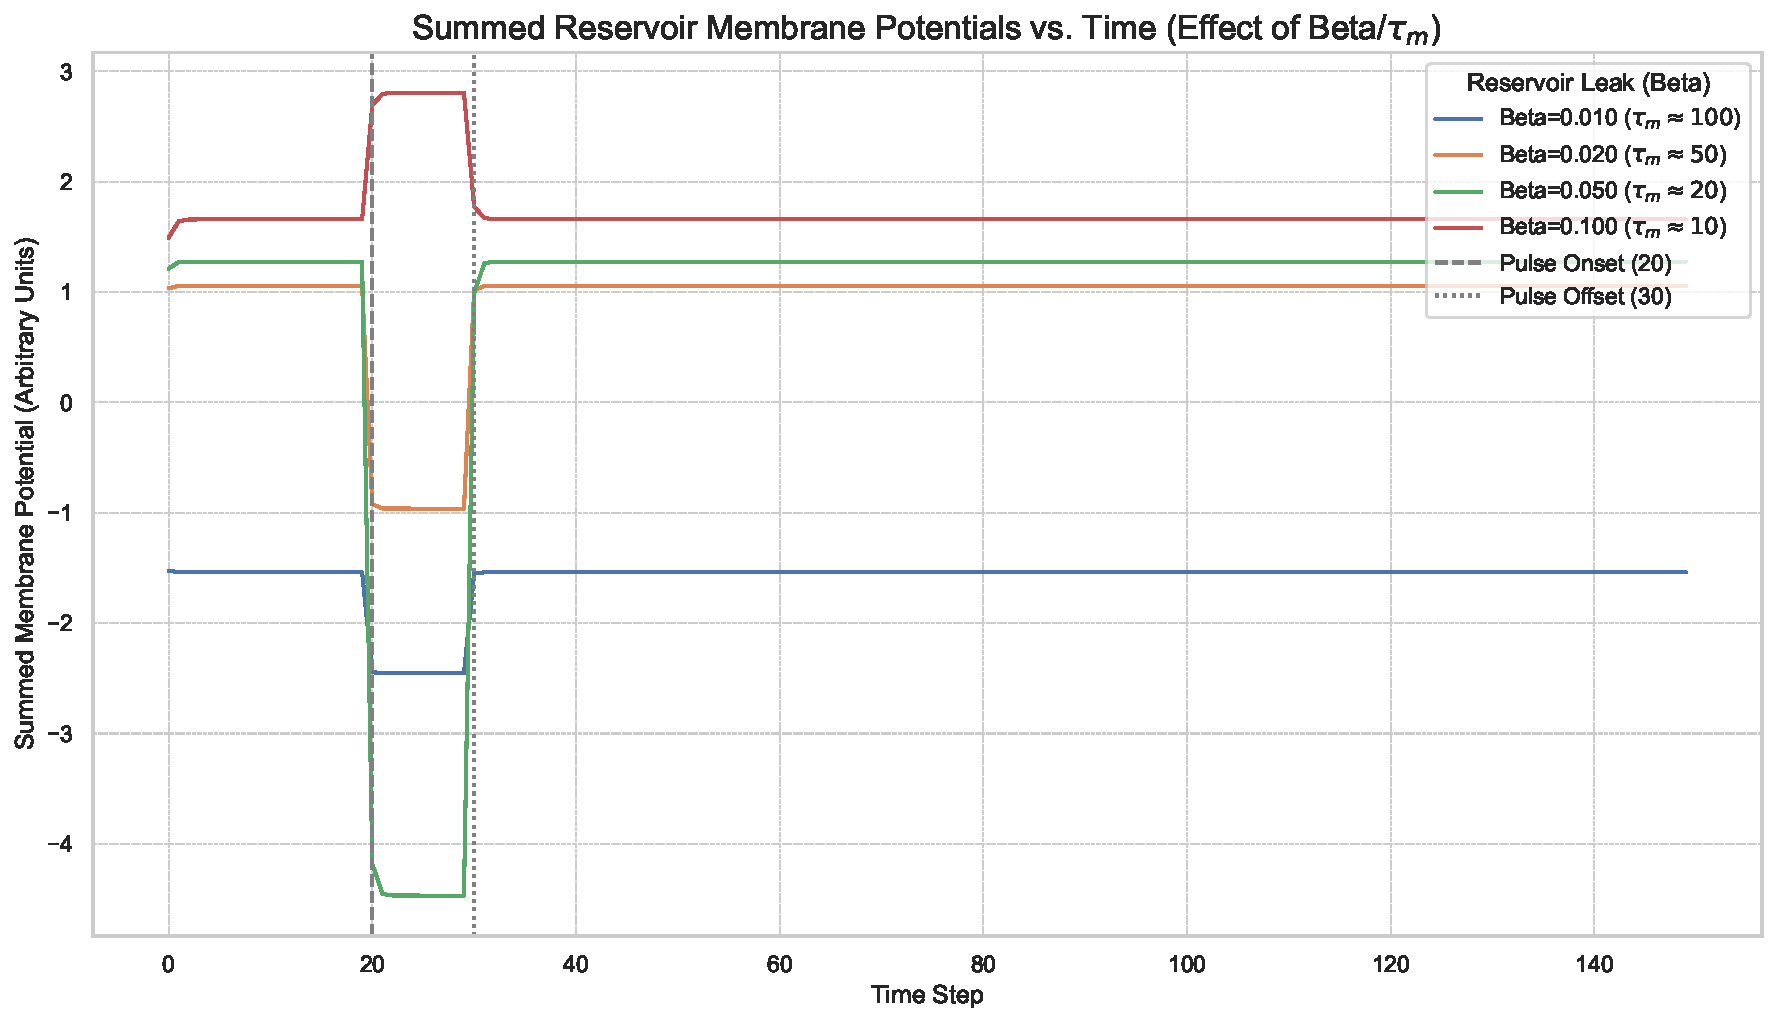
\includegraphics[width=0.9\textwidth]{pictures/chLSM/lsm_summed_activity_beta_comparison.pdf}
    \caption{Summed reservoir membrane potentials over time for different $\beta$ values. The input pulse was active from time step 20 to 30. Smaller $\beta$ (larger $\tau_m$) produces more sustained responses, consistent with first-order low-pass filtering.}
    \label{fig:summed_beta_response}
\end{figure}

\begin{figure}[H]
    \centering
    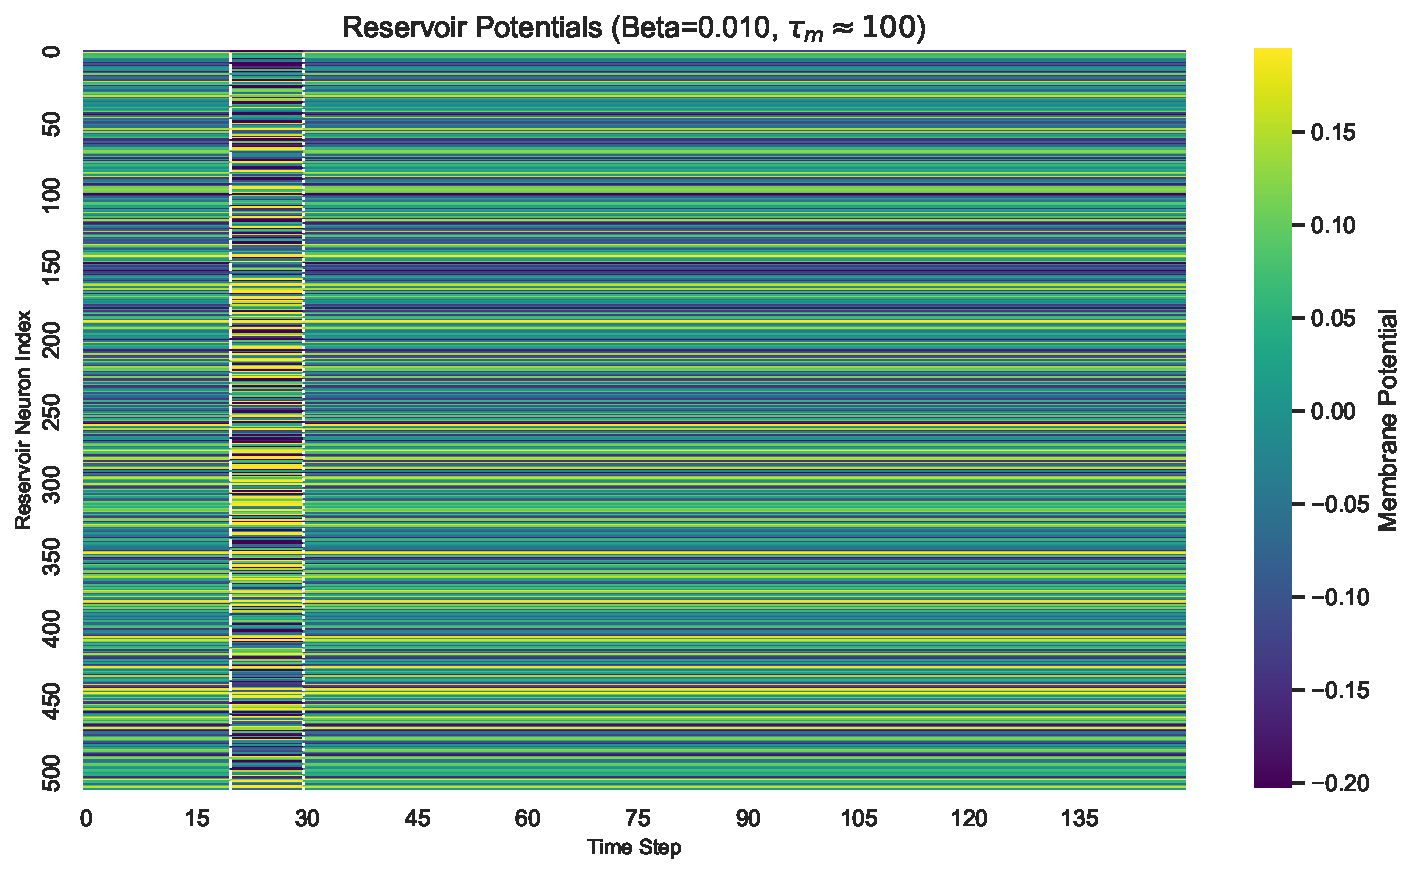
\includegraphics[width=0.8\textwidth]{pictures/chLSM/lsm_heatmap_beta_0p01.pdf}
    \caption{Heatmap of membrane potentials for all 512 reservoir neurons with $\beta = 0.010$ ($\tau_m \approx 100$). Activity is sustained across many neurons long after the input pulse, reflecting long temporal integration.}
    \label{fig:heatmap_beta_slow}
\end{figure}

\begin{figure}[H]
    \centering
    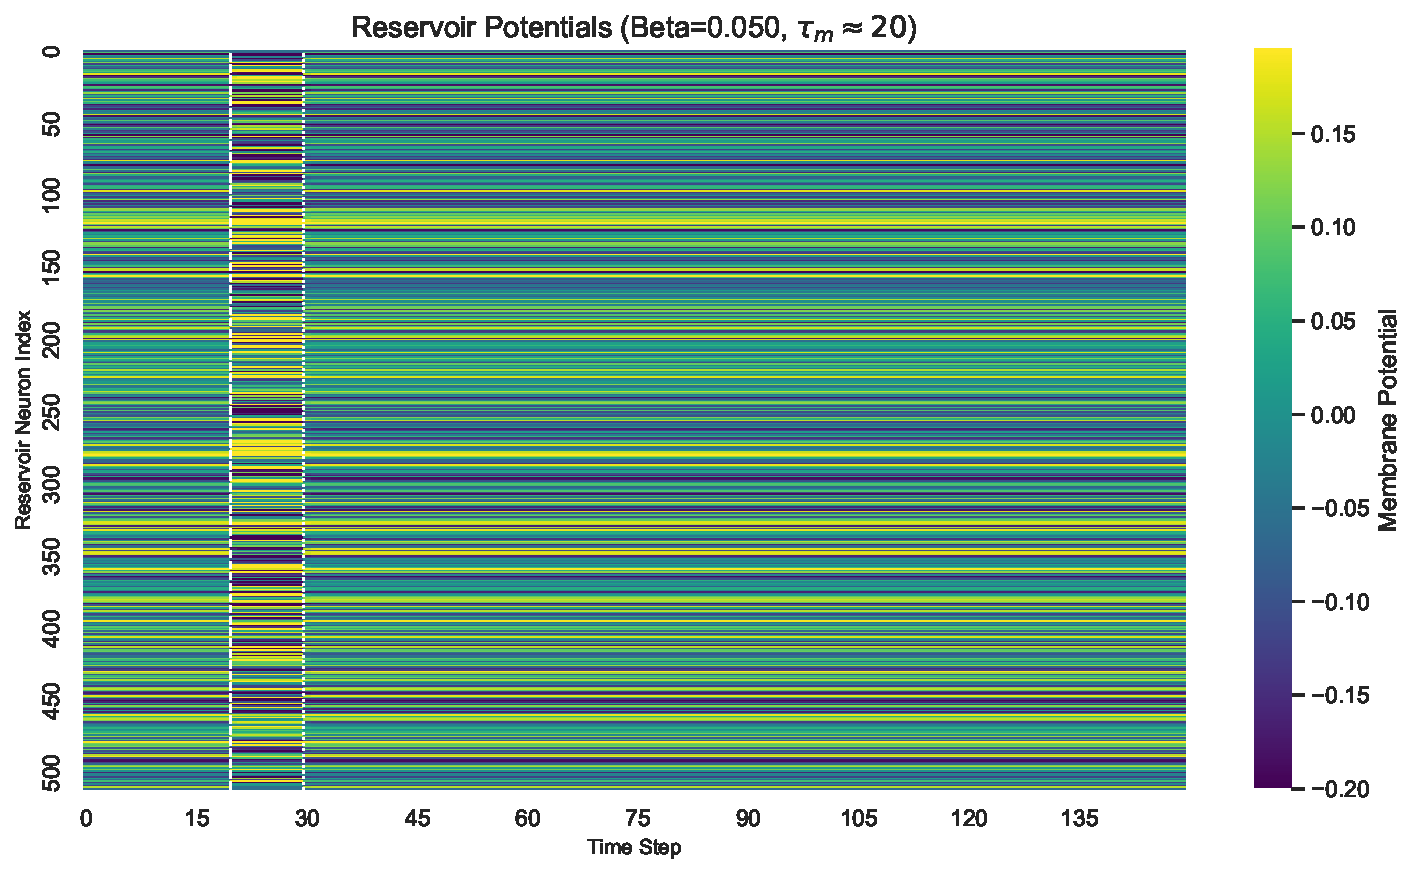
\includegraphics[width=0.8\textwidth]{pictures/chLSM/lsm_heatmap_beta_0p05.pdf}
    \caption{Heatmap of membrane potentials for all 512 reservoir neurons with $\beta = 0.050$ ($\tau_m \approx 20$). Activation is more transient, with most neurons returning to baseline within 30--40 steps of pulse offset.}
    \label{fig:heatmap_beta_fast}
\end{figure}

\subsection{Discussion and Significance}

The sweep shows that response persistence changes systematically with $\beta$ in this realization. For a single exponential decay, the remaining fraction after $k$ time constants is $e^{-k}\approx\{0.368,0.135,0.050,0.018\}$ for $k\in\{1,2,3,4\}$. The summed-potential traces are qualitatively consistent with that expectation \cite{gerstner_spiking_2002}, although the recurrent, thresholded population is not an exact single-exponential system.

The aggregate and unit-level plots are both consistent with a contribution from the decay parameter. A causal decomposition would require an ablation of recurrence or a matched analytic model, which was not performed here.

$\beta=0.05$ was retained as a provisional engineering choice because its response persisted through the immediate post-pulse interval without remaining elevated for the full simulated epoch. No mutual information, formal memory capacity, or nonlinear capacity was estimated in this module.

For the tested pulse, the $\beta=0.05$ response is concentrated near the window later sampled in Module~3. This alignment motivates, but does not independently validate, the subsequent feature window.


%% ===================================================================
%% MODULE 2
%% ===================================================================
\section{Module 2: Input Strength, Firing Threshold, and the Transition to Spiking}
\label{sec:module2}

\subsection{Theoretical Motivation}

Module~1 described temporal persistence. Module~2 asks how the observed response changes when the selected threshold does or does not permit spikes under the tested input amplitudes.

When no unit crosses threshold, the spike-dependent recurrent term is zero and the implemented update is linear apart from the nonnegative membrane floor. Different input-weight realizations can therefore give different aggregate projections of the same pulse. Such seed dependence is expected in a random-feature model and is not, by itself, evidence of instability.

Threshold crossing introduces a piecewise nonlinearity. In the implementation used here, the threshold is subtracted from the updated membrane, the result is floored at zero, and the retained membrane term is cleared on the next step for a unit that spiked. This is not a reset of every spike to one identical post-spike value, and the present design does not estimate whether it reduces seed sensitivity.

The practical criterion used here is simpler than a proof of separation or approximation: the selected configuration should emit nonzero, amplitude-dependent spikes that can be summarized by the downstream feature extractor.

This module empirically characterizes both regimes and tests which provides a more reliable basis for downstream feature extraction, a decision with direct architectural consequences for ARSPI-Net.

\subsection{Experimental Design}

Two threshold conditions were examined: $M_{\text{th}} = 1.0$ (high threshold, suppressing spiking) and $M_{\text{th}} = 0.5$ (low threshold, enabling spiking). For each condition, input pulse amplitudes of 0.6, 1.2, and 2.0 were applied (all other parameters as in Module~1, with $\beta = 0.05$). To assess initialization sensitivity in the subthreshold regime, the $M_{\text{th}} = 1.0$ condition was repeated across $N_{\text{instances}} = 5$ independent LSM instances, each with a newly initialized $\mathbf{W}^{\text{in}}$ (Xavier uniform) but identical $\mathbf{W}^{\text{rec}}$ and neuron parameters. The $M_{\text{th}} = 0.5$ condition was analyzed from a single representative instance, consistent with the exploratory objective of identifying a functional spiking regime.

Key observables included the summed membrane potential $V_{\text{summed}}[t]$ (Equation~\ref{eq:v_summed}), the instantaneous population firing rate $R[t] = (1/N_{\text{res}}) \sum_i S_i[t]$, the total spike count during the pulse window (steps 20--30), and the peak population firing rate.

\subsection{Results: Subthreshold Regime \texorpdfstring{($M_{\text{th}} = 1.0$)}{(threshold = 1.0)}}
\label{sec:subthreshold_results}

Across the five high-threshold input-weight realizations, the aggregate membrane summaries varied visibly. Peak deflection was non-monotonic in one realization, decreased with amplitude in two, showed a plateau followed by a change in one, and was nearly flat in one (Figures~\ref{fig:instance1_thresh1_standalone}--\ref{fig:instance5_thresh1_standalone}). Figure~\ref{fig:summary_thresh1_new} summarizes these five descriptive observations; with only five realizations, it is not a population estimate of seed robustness.

Each $\mathbf{W}^{\text{in}}$ realization defines a different random projection, so seed-dependent aggregate responses are unsurprising \cite{Norton2020_NextGenRC,Lukosevicius2009_Reservoir}. The observed input--summary relationship is therefore a property of both the stated architecture and its realized weights.

\begin{figure}[H]
    \centering
    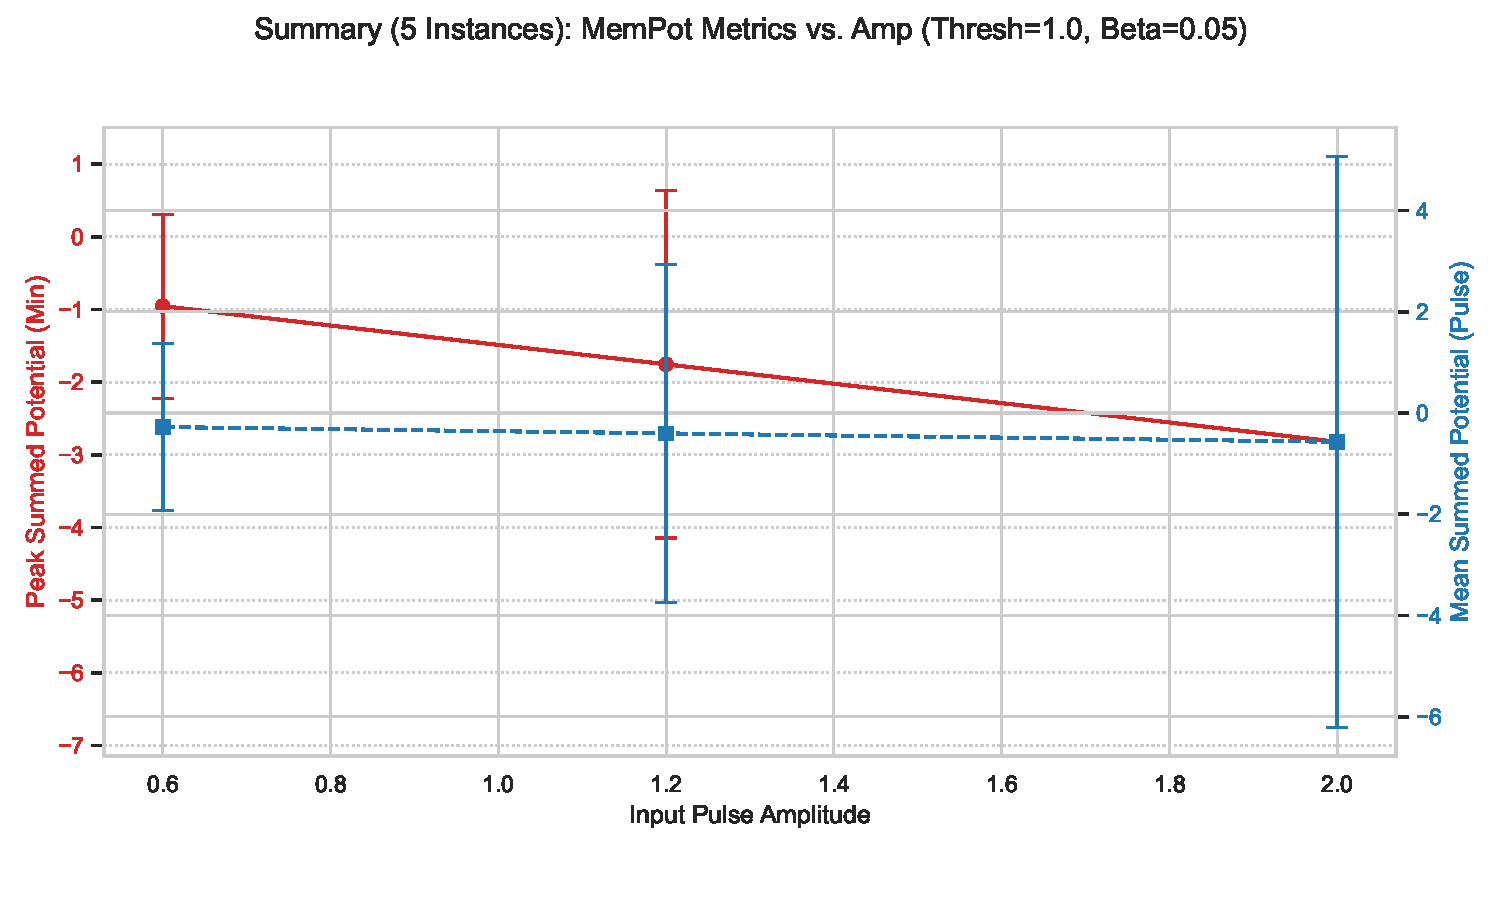
\includegraphics[width=0.7\textwidth]{pictures/chLSM/summary_mempot_metrics_thresh1p0.pdf}
    \caption{Summary of subthreshold metrics versus input amplitude across 5 network instances ($M_{\text{th}} = 1.0$, $\beta = 0.05$). Error bars represent standard deviation. The large variability reflects the sensitivity of continuous-valued trajectories to the random input projection.}
    \label{fig:summary_thresh1_new}
\end{figure}

\begin{figure}[H]
    \centering
    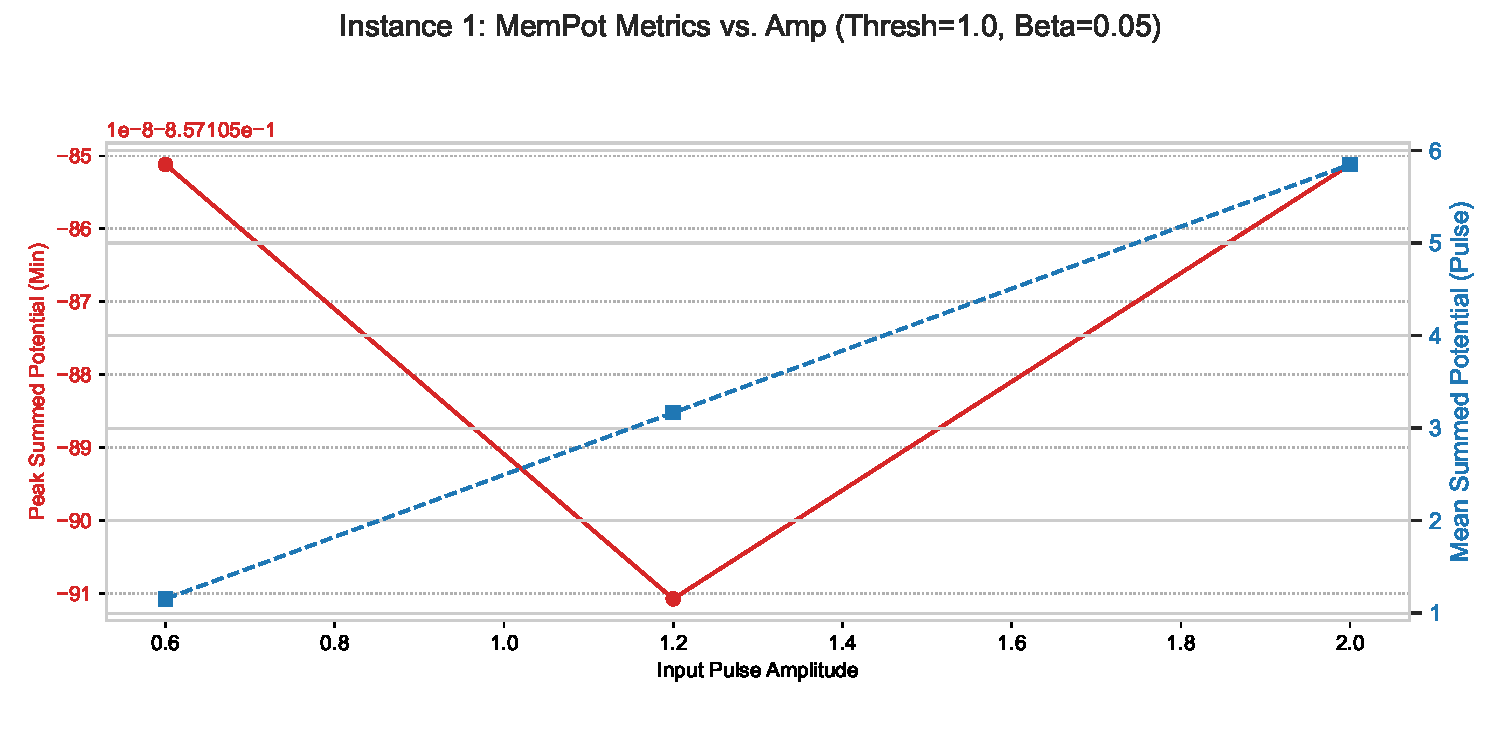
\includegraphics[width=0.7\textwidth]{pictures/chLSM/instance1_mempot_metrics_thresh1p0.pdf}
    \caption{Instance 1: Non-monotonic peak deflection, monotonically increasing mean potential.}
    \label{fig:instance1_thresh1_standalone}
\end{figure}

\begin{figure}[H]
    \centering
    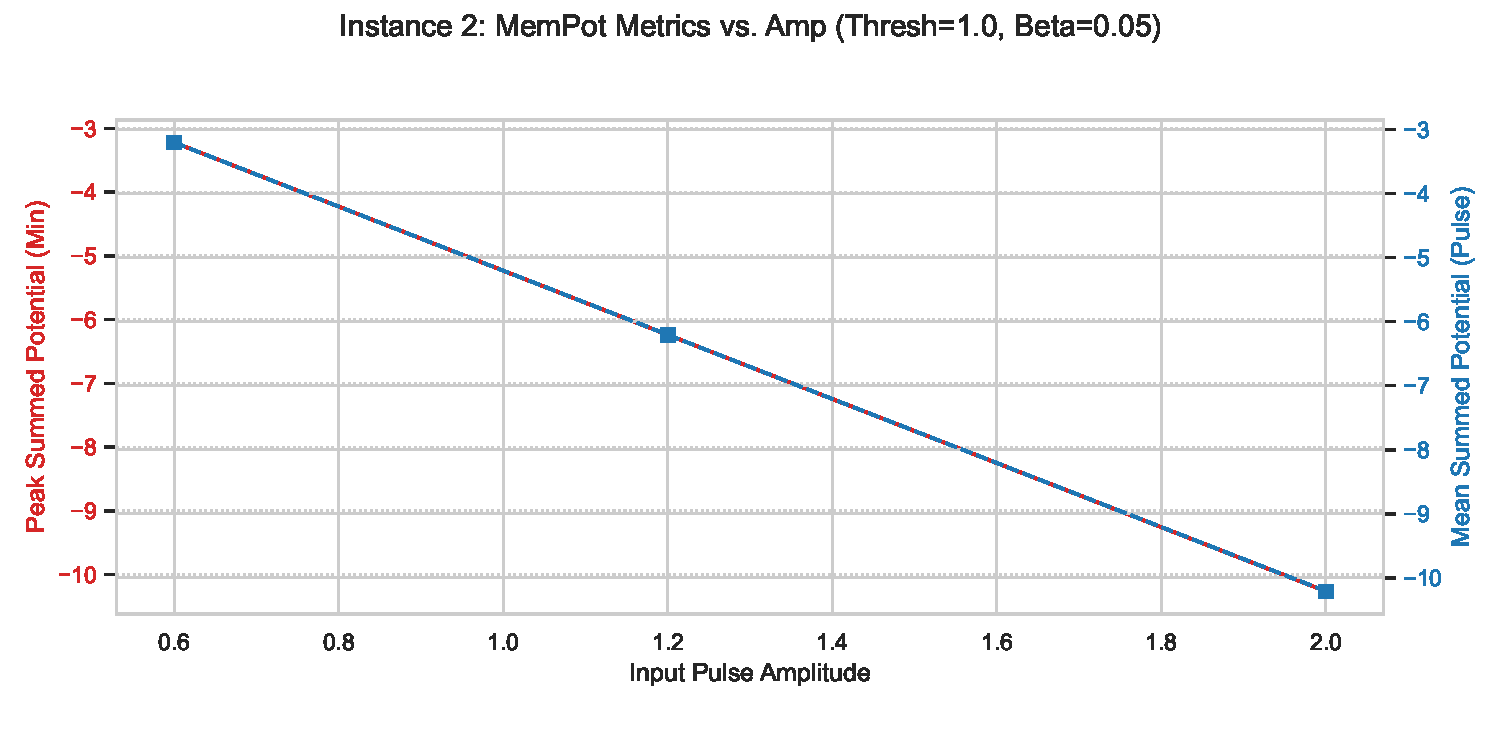
\includegraphics[width=0.7\textwidth]{pictures/chLSM/instance2_mempot_metrics_thresh1p0.pdf}
    \caption{Instance 2: Both metrics show strong monotonic decrease with input amplitude.}
    \label{fig:instance2_thresh1_standalone}
\end{figure}

\begin{figure}[H]
    \centering
    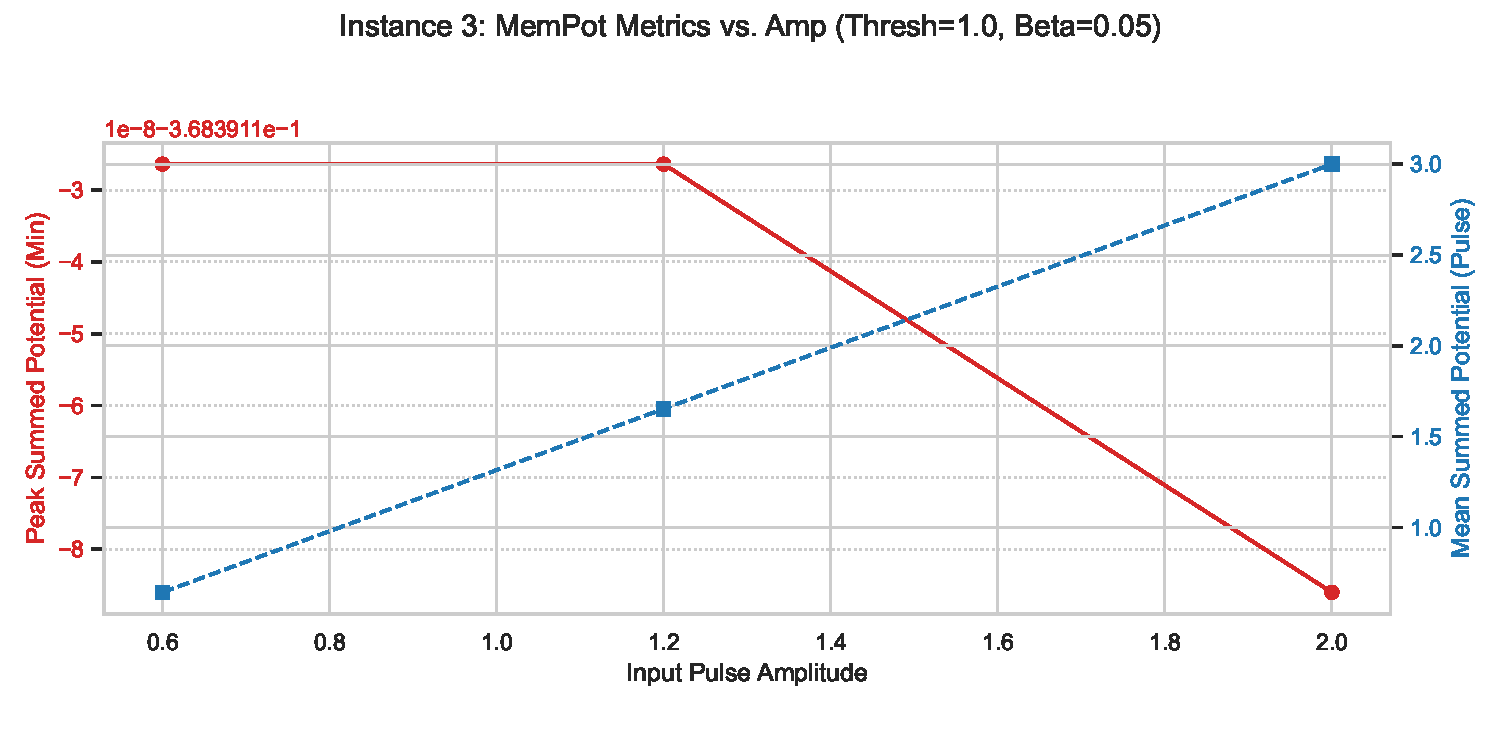
\includegraphics[width=0.7\textwidth]{pictures/chLSM/instance3_mempot_metrics_thresh1p0.pdf}
    \caption{Instance 3: Plateau followed by sharp decrease; monotonically increasing mean.}
    \label{fig:instance3_thresh1_standalone}
\end{figure}

\begin{figure}[H]
    \centering
    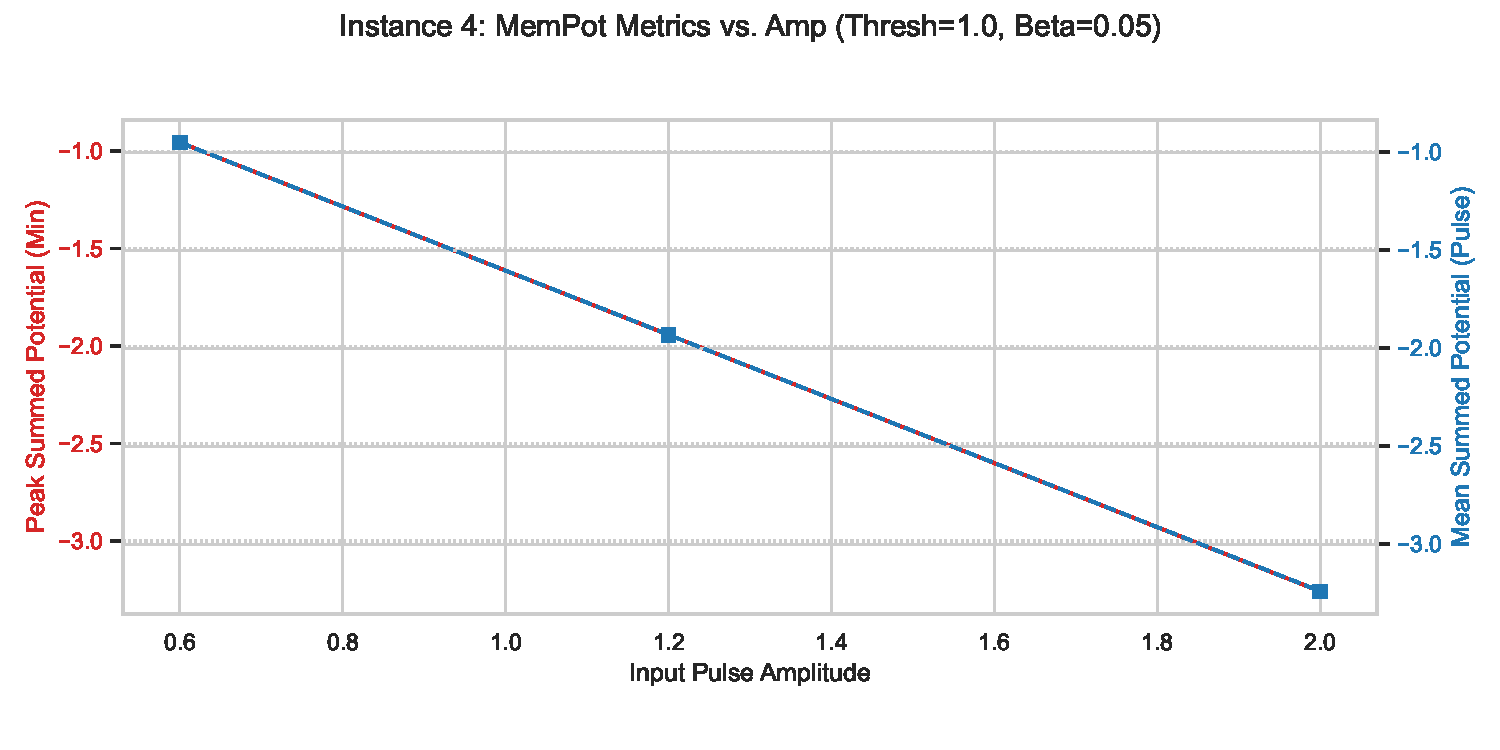
\includegraphics[width=0.7\textwidth]{pictures/chLSM/instance4_mempot_metrics_thresh1p0.pdf}
    \caption{Instance 4: Consistent monotonic decrease, similar to Instance 2.}
    \label{fig:instance4_thresh1_standalone}
\end{figure}

\begin{figure}[H]
    \centering
    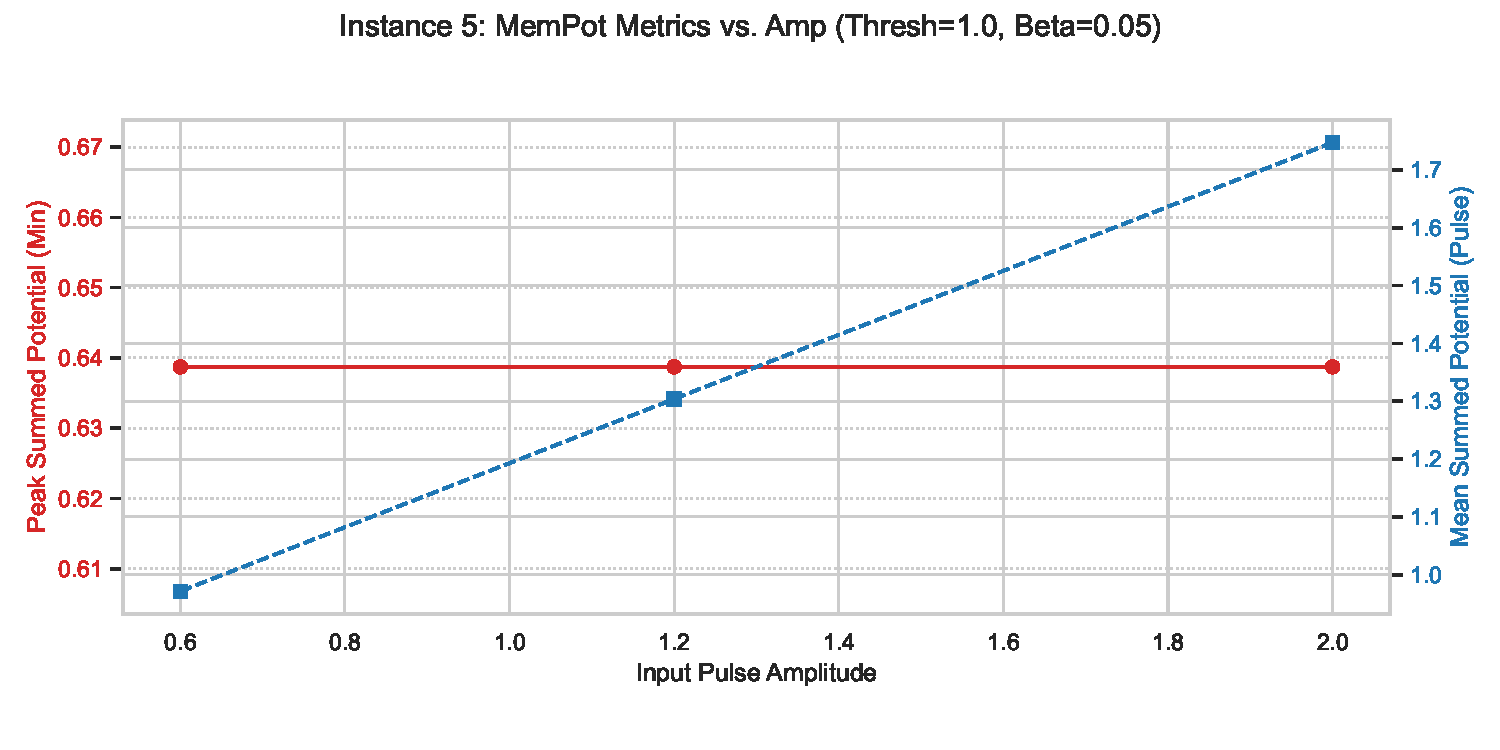
\includegraphics[width=0.7\textwidth]{pictures/chLSM/instance5_mempot_metrics_thresh1p0.pdf}
    \caption{Instance 5: Nearly constant peak deflection; monotonically increasing mean.}
    \label{fig:instance5_thresh1_standalone}
\end{figure}

\subsection{Results: Spiking Regime \texorpdfstring{($M_{\text{th}} = 0.5$)}{(threshold = 0.5)}}
\label{sec:spiking_results}

In the one low-threshold realization examined, lowering $M_{\text{th}}$ to 0.5 produced spike activity that increased with input amplitude. Because this condition was not repeated across seeds, the result does not establish robustness or reproducibility across initializations.

The archived summed-potential figure (Figure~\ref{fig:m2_summed_mempot_thresh0p5_actual}) has positive deflections at amplitudes 0.6 and 1.2 and negative values at amplitude 2.0 during the pulse. Because the audited implementation floors each retained membrane value at zero, this sign change cannot be attributed to that implementation. Figure~\ref{fig:m2_mempot_metrics_thresh0p5_actual} is retained only to document the legacy run.

In the archived firing-rate figure (Figure~\ref{fig:m2_pop_firing_rate_thresh0p5_actual}), amplitude 0.6 produces almost no spikes, amplitude 1.2 produces about five spikes during the pulse, and amplitude 2.0 produces about 170. This is an amplitude ordering in one legacy realization, not a calibrated population frequency--current curve or a cross-seed result.

\begin{figure}[H]
    \centering
    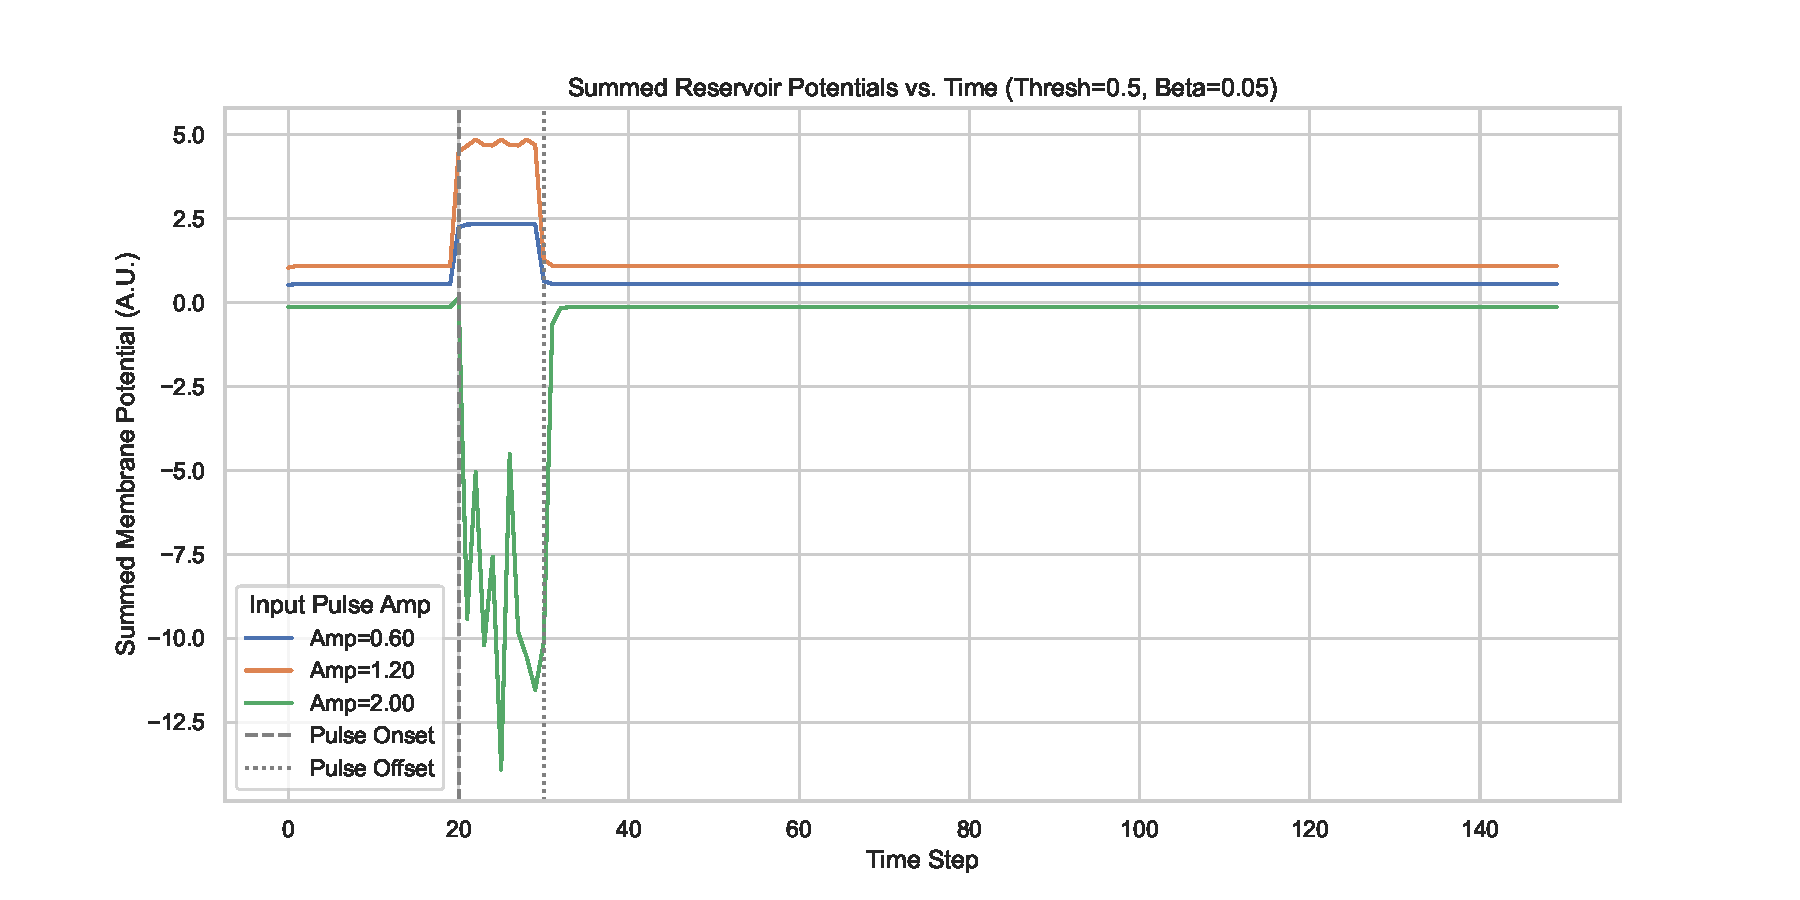
\includegraphics[width=0.9\textwidth]{pictures/chLSM/summed_mempot_thresh0p5.pdf}
    \caption{Archived summed membrane potentials in the low-threshold run ($M_{\text{th}} = 0.5$, $\beta = 0.05$). The negative retained values are incompatible with the audited nonnegative-floor update, so the plot is a legacy observation rather than current-model verification.}
    \label{fig:m2_summed_mempot_thresh0p5_actual}
\end{figure}

\begin{figure}[H]
    \centering
    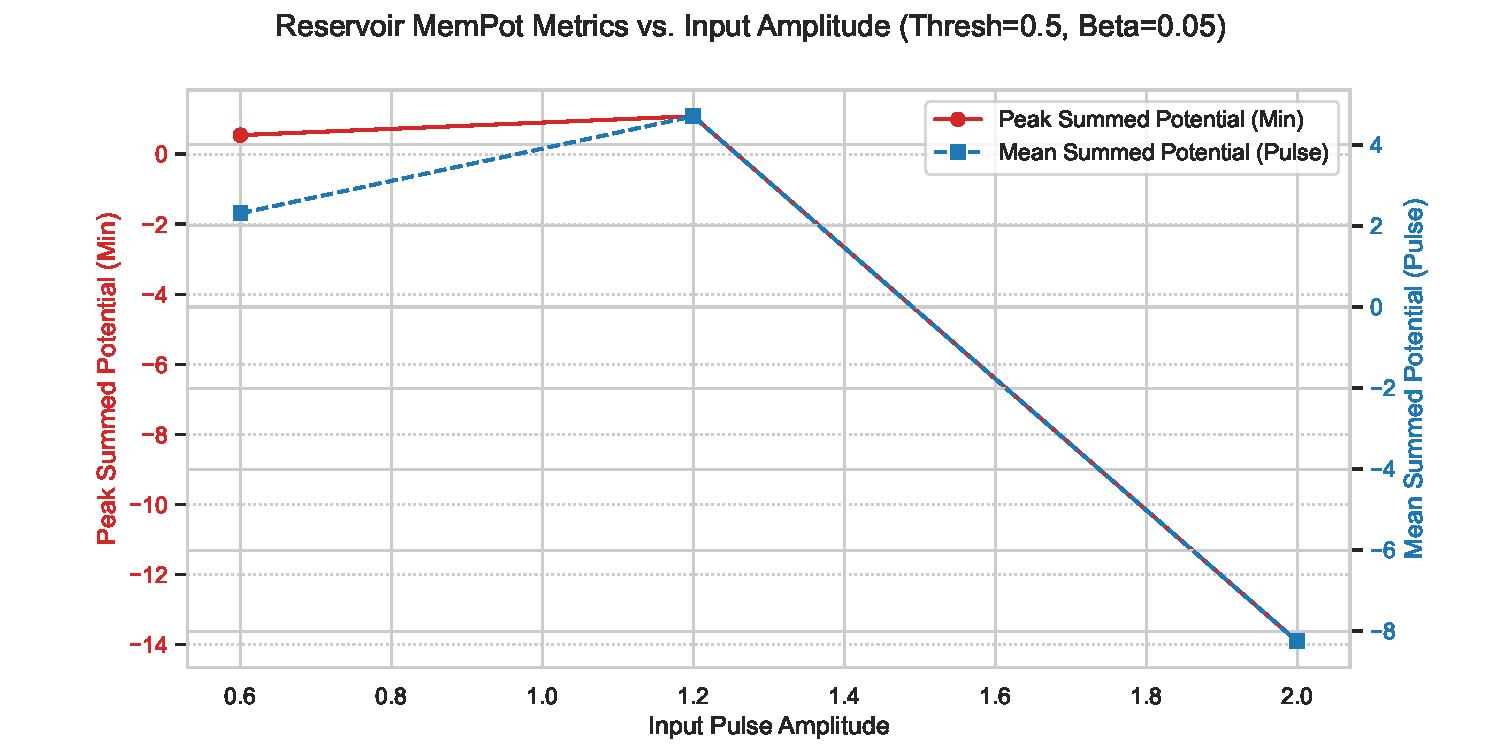
\includegraphics[width=0.8\textwidth]{pictures/chLSM/mempot_metrics_vs_amp_thresh0p5.pdf}
    \caption{Archived membrane summaries versus input amplitude in the low-threshold run. The sign change at the largest amplitude inherits the legacy-update mismatch.}
    \label{fig:m2_mempot_metrics_thresh0p5_actual}
\end{figure}

\begin{figure}[H]
    \centering
    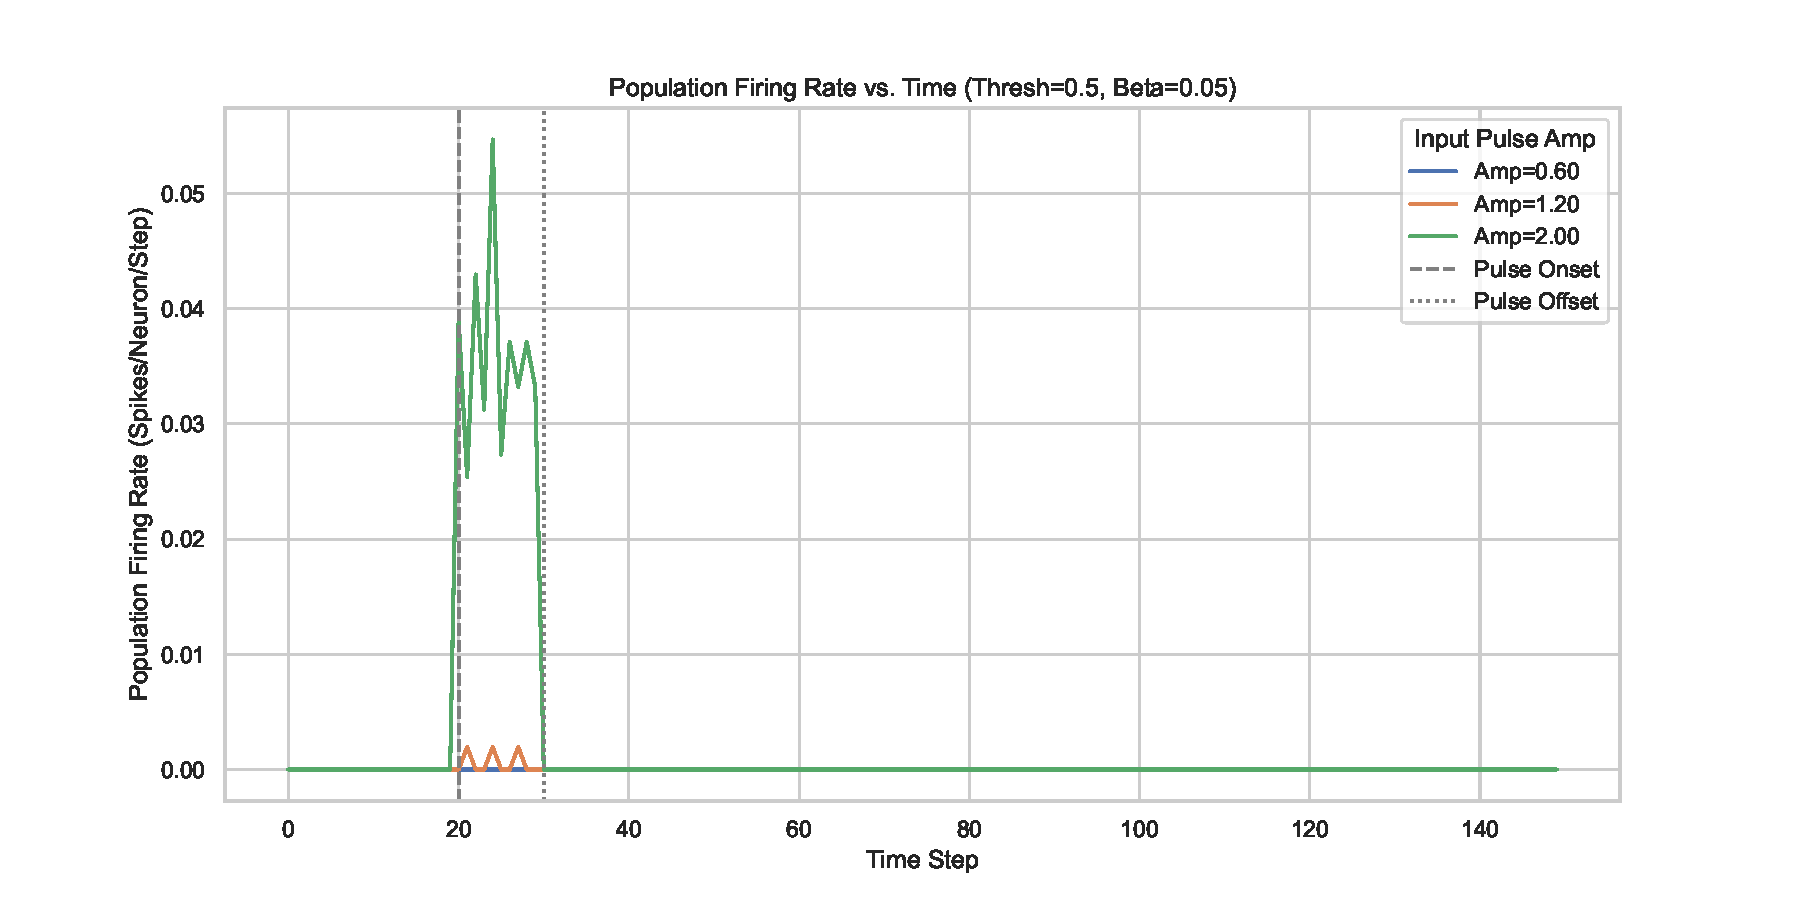
\includegraphics[width=0.9\textwidth]{pictures/chLSM/pop_firing_rate_thresh0p5.pdf}
    \caption{Population firing rate versus time for three input amplitudes in one reservoir realization ($M_{\text{th}}=0.5$, $\beta=0.05$). Spiking increased with input strength in this realization.}
    \label{fig:m2_pop_firing_rate_thresh0p5_actual}
\end{figure}

\begin{figure}[H]
    \centering
    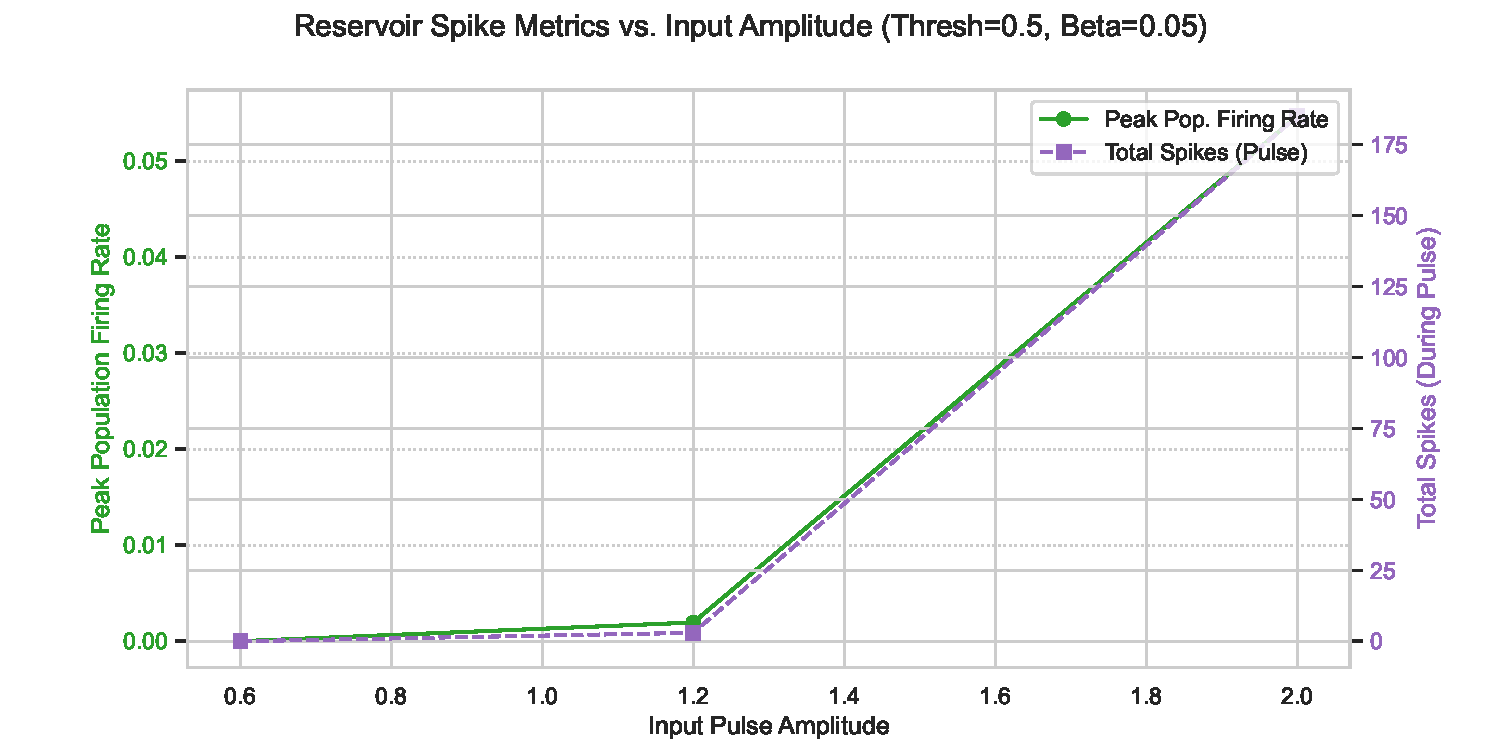
\includegraphics[width=0.8\textwidth]{pictures/chLSM/spike_metrics_vs_amp_thresh0p5.pdf}
    \caption{Archived peak population firing rate and total spike count versus input amplitude in one realization. The three points show an amplitude ordering but do not estimate a population frequency--current curve.}
    \label{fig:m2_spike_metrics_thresh0p5_actual}
\end{figure}

\subsection{Discussion and Significance}
\label{sec:module2_discussion}

The module documents different response summaries under the two threshold settings, while its asymmetric seed sampling limits between-regime inference.

\subsubsection{The Regularizing Role of the Spiking Nonlinearity}

The high-threshold plots show that aggregate membrane summaries depend on the random projection. This does not make the regime intrinsically unreliable: random-feature systems are normally calibrated with their realized weights. It does mean that the summaries should not be presented as architecture-only quantities.

The low-threshold update adds thresholding and reset to the response, producing a nonlinear spike-count feature. A matched multi-seed experiment would be needed to determine whether that feature is more consistent across realizations than the high-threshold membrane summaries.

\subsubsection{The Population Rate Code and Its Engineering Significance}

Continuous-time LIF models have a monotonic frequency--current relationship above threshold \cite{gerstner_spiking_2002,dayan2001}. The custom discrete update here is not identical to that analytic model, but the observed increase in total spikes and peak population rate with amplitude is qualitatively consistent with it. Spike counts are therefore retained as candidate downstream features.

The population firing-rate vector $\mathbf{r}=[r_1,\ldots,r_{N_{\text{res}}}]$ is a high-dimensional summary whose components reflect different input and recurrent weights. The tested amplitude sweep shows that this summary is nonconstant and graded in the selected realization; it does not quantify how much input information is preserved.

Robust spike coding has been demonstrated for networks designed around coordinated error correction \cite{Boerlin2013_PredictiveCoding}. The present random reservoir does not implement that construction, so the citation supplies context rather than evidence that this reservoir has the same robustness property.

\subsubsection{Implications for ARSPI-Net}

The threshold $M_{\text{th}}=0.5$ was adopted provisionally because it produced a nonzero, amplitude-dependent spike code in the selected realization and is compatible with binned spike-count features. Cross-seed superiority over the high-threshold setting remains untested in this module.


%% ===================================================================
%% MODULE 3
%% ===================================================================
\section{Module 3: Temporal Localization of Discriminative Information}
\label{sec:module3}

\subsection{Theoretical Motivation}

Modules~1 and 2 produced provisional temporal and threshold settings. The next question is which tested window yields distinct mean firing-rate vectors for the two synthetic responses.

Mean firing rate discards within-window timing and correlations, so failure of this readout would not prove that the full state is identical. No mutual information is estimated in this module.

The single-unit decay approximation suggests that an early window may retain a larger pulse response than a late window, while recurrence can alter that pattern. The experiment compares readout summaries; it does not prove that the full reservoir has fading memory or determine whether sustained recurrent patterns exist.

The comparison provides one input to window selection. With only four prespecified windows and two unique signals, it cannot identify an optimal window or estimate memory capacity.

\subsection{Experimental Design}

A binary deterministic contrast was defined: Class~0 (pulse amplitude 1.2) versus Class~1 (pulse amplitude 2.0). The generator introduced no noise, jitter, or other within-class variation, so the 200 stored rows per class were repeated copies of one class-specific response rather than independent trials. The effective number of unique input signals was therefore two. Mean firing rates from the 512-unit response were extracted from four temporal windows:
\begin{itemize}
    \item \textbf{Early Window}: time steps 20--50 (stimulus onset plus 20 post-stimulus steps)
    \item \textbf{Late Window}: time steps 50--100
    \item \textbf{Full Response Window}: time steps 20--150
    \item \textbf{Entire Trial}: time steps 0--150
\end{itemize}
Each window produced a 512-dimensional feature vector per stored row. Logistic regression with L2 regularization ($C=0.1$) was evaluated using five stratified folds, with \texttt{StandardScaler} fitted on each training fold. Because identical rows occur in both training and test folds, these scores are a deterministic separability check and must not be interpreted as independent out-of-sample validation.

\subsection{Results}

For the two unique responses, the Early Window, Full Response Window, and Entire Trial feature vectors were separable by the fitted readout (reported fold accuracy $1.000\pm0.000$), whereas the Late Window vectors were not distinguished (reported accuracy $0.500\pm0.000$; Figure~\ref{fig:m3_accuracy_cv_comparison}). The zero fold variance is expected from duplicated deterministic rows and is not a precision estimate.

The confusion matrices in Figure~\ref{fig:m3_confusion_matrices_cv} count stored duplicates, not 400 independent observations. They show that the classifier assigned all duplicates correctly when the early response was included and assigned all Late Window duplicates to Class~0 when the two late feature vectors were not distinguished by this readout.

\begin{figure}[H]
    \centering
    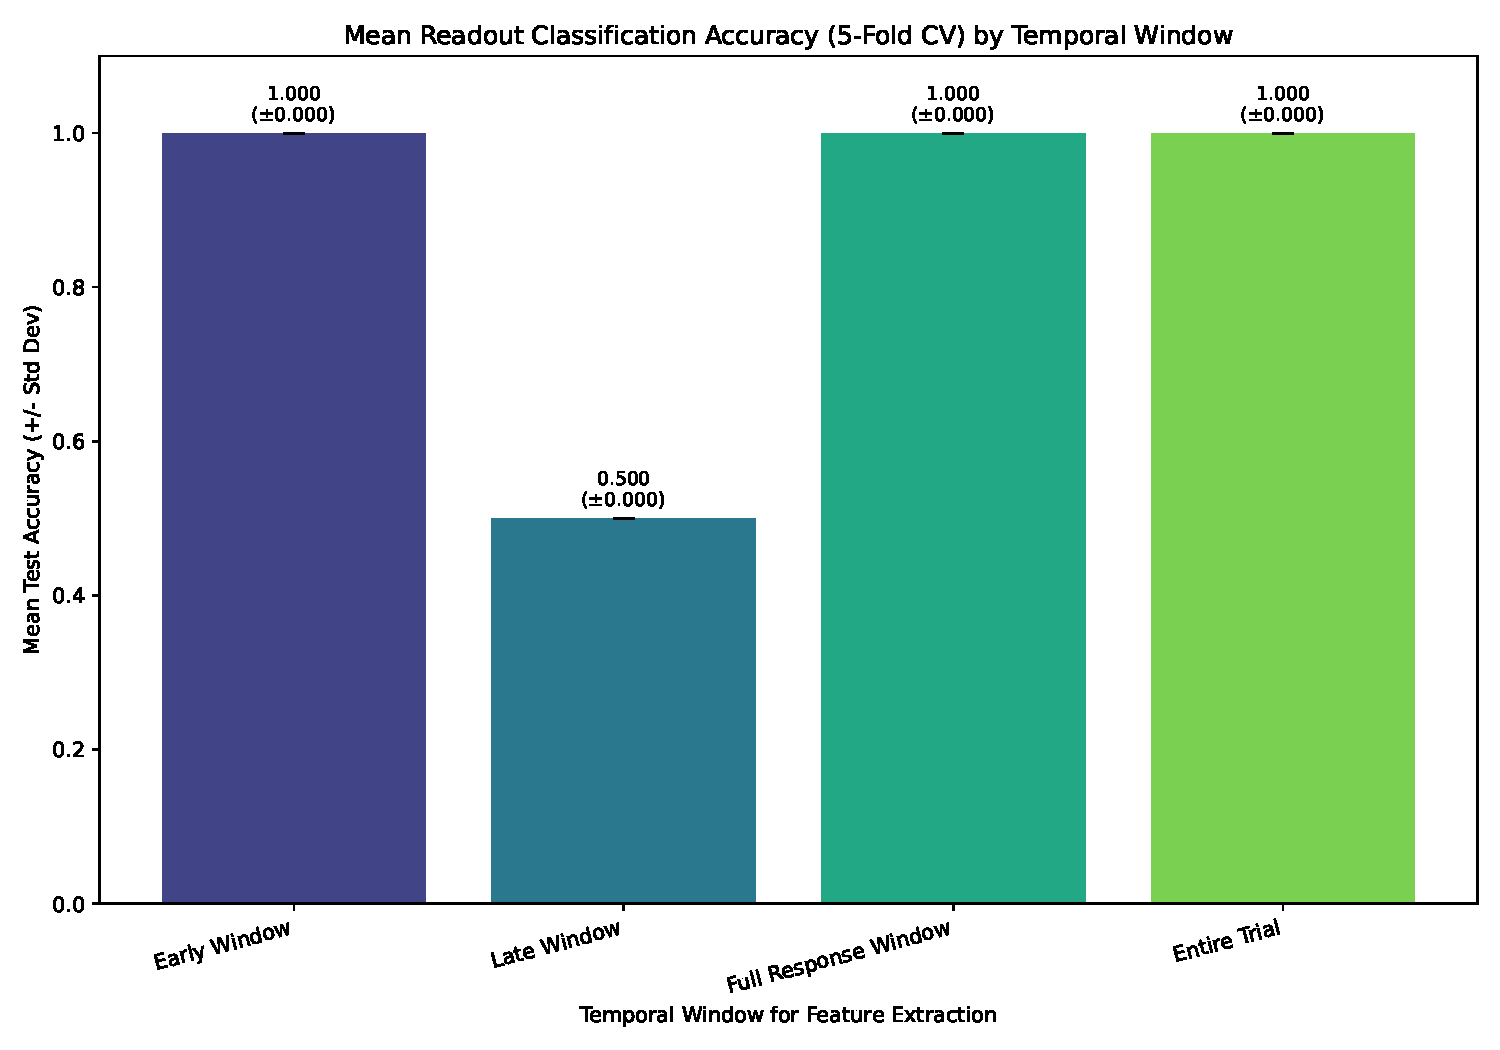
\includegraphics[width=0.9\textwidth]{pictures/chLSM/readout_accuracy_cv_comparison.pdf}
    \caption{Reported five-fold accuracy for readouts trained on deterministic, duplicated feature rows. The two unique class responses were separable when the early response was included but not from the Late Window mean rates. These are separability checks, not independent generalization estimates.}
    \label{fig:m3_accuracy_cv_comparison}
\end{figure}

\begin{figure}[H]
    \centering
    \begin{subfigure}{0.48\textwidth}
        \centering
        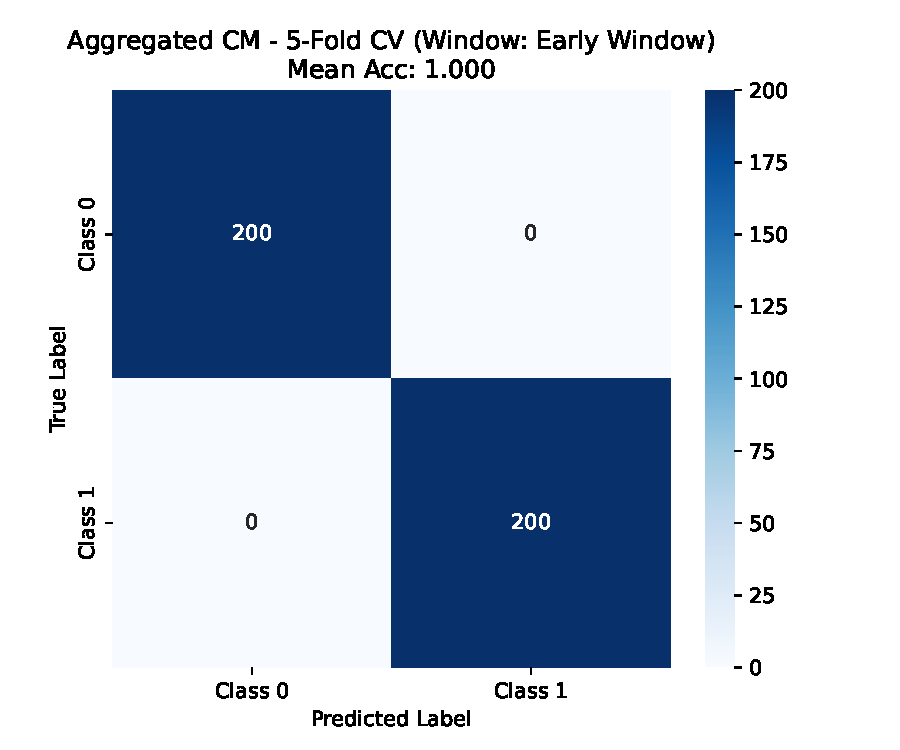
\includegraphics[width=\linewidth]{pictures/chLSM/confusion_matrix_cv_window_early_window.pdf}
        \caption{Early Window (Acc: 1.000)}
        \label{fig:m3_cm_cv_early}
    \end{subfigure}
    \hfill
    \begin{subfigure}{0.48\textwidth}
        \centering
        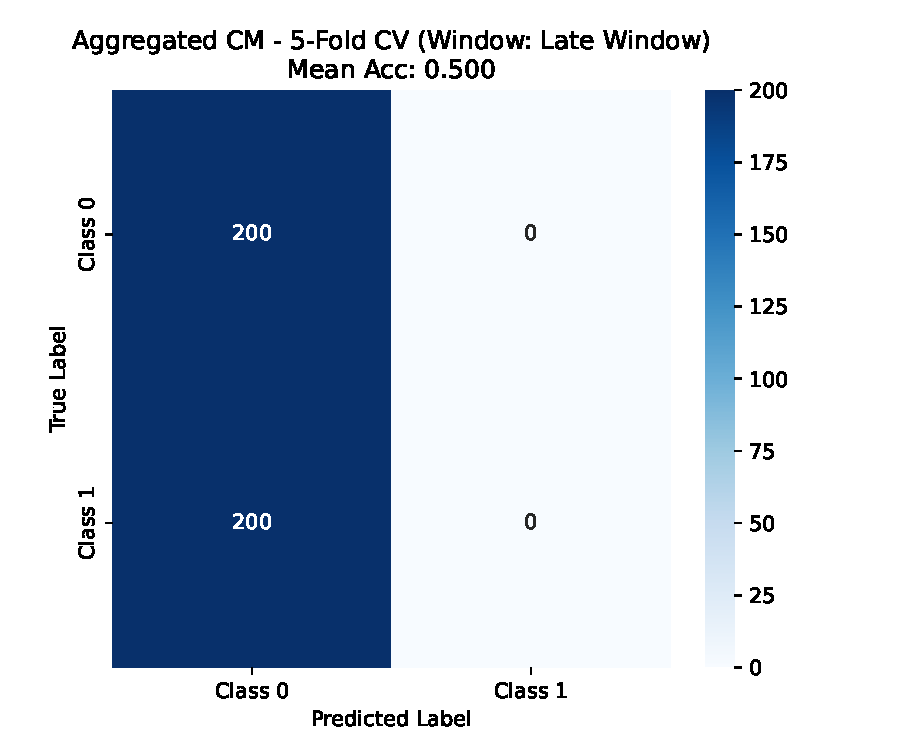
\includegraphics[width=\linewidth]{pictures/chLSM/confusion_matrix_cv_window_late_window.pdf}
        \caption{Late Window (Acc: 0.500)}
        \label{fig:m3_cm_cv_late}
    \end{subfigure}
    \vspace{1em}
    \begin{subfigure}{0.48\textwidth}
        \centering
        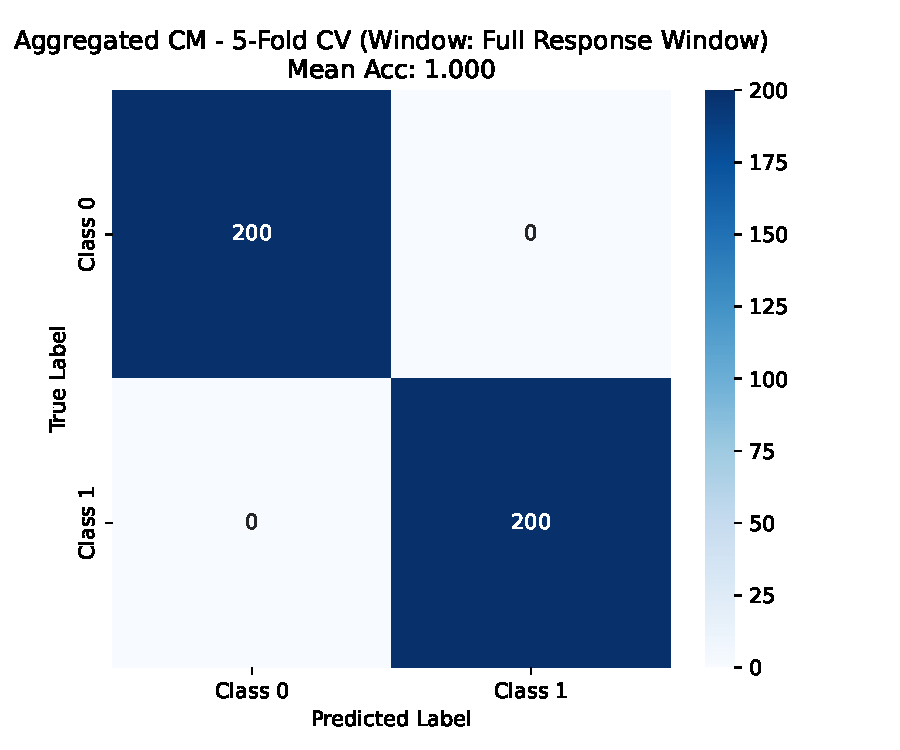
\includegraphics[width=\linewidth]{pictures/chLSM/confusion_matrix_cv_window_full_response_window.pdf}
        \caption{Full Response Window (Acc: 1.000)}
        \label{fig:m3_cm_cv_full}
    \end{subfigure}
    \hfill
    \begin{subfigure}{0.48\textwidth}
        \centering
        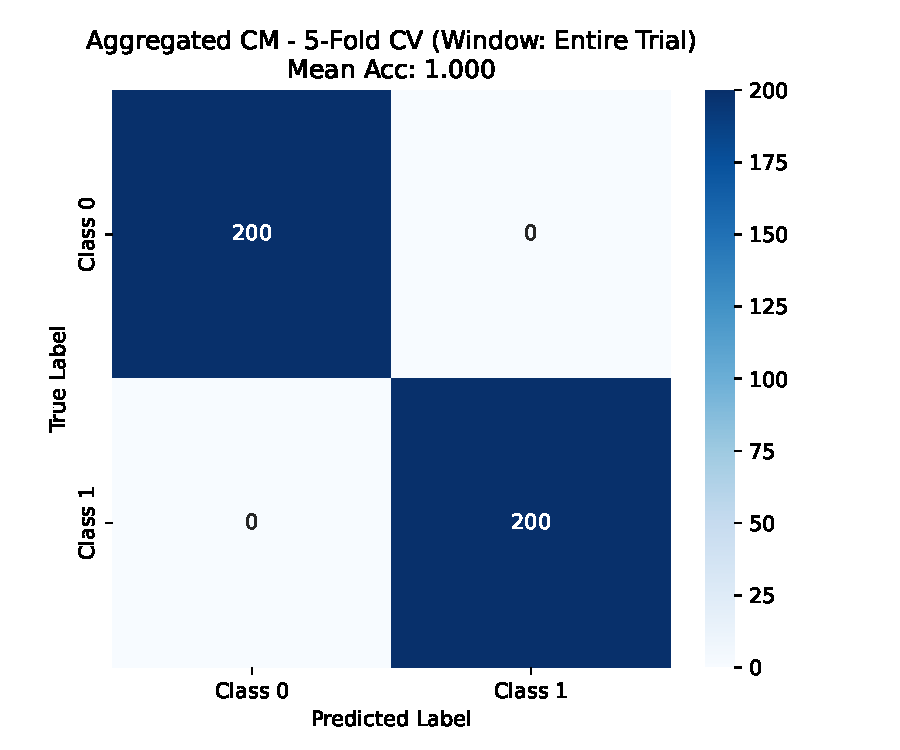
\includegraphics[width=\linewidth]{pictures/chLSM/confusion_matrix_cv_window_entire_trial.pdf}
        \caption{Entire Trial (Acc: 1.000)}
        \label{fig:m3_cm_cv_entire}
    \end{subfigure}
    \caption{Aggregated confusion matrices across five folds. Counts reflect duplicated deterministic rows (200 copies per class), not independent trials. $\beta=0.05$, $M_{\text{th}}=0.5$.}
    \label{fig:m3_confusion_matrices_cv}
\end{figure}

\subsection{Discussion and Significance}

\subsubsection{The Biophysical Basis of Information Decay}

The Late Window result is consistent with fading memory. Under a single-unit exponential approximation with $\beta=0.05$ ($\tau_m\approx20$ steps), a perturbation would fall to about 36.8\% after one time constant and about 3\% after 3.5 time constants. The classifier result alone does not establish that this mechanism caused the loss of separability in the full recurrent system.

After external drive ceases, activity reflects both decay and autonomous recurrent dynamics \cite{Sussillo2009,Barak2017}. In this realization the 50-step mean-rate readout did not distinguish the two late responses. The experiment did not identify a common attractor or test whether fine spike timing retained class structure.

\subsubsection{What Information Decay Does and Does Not Imply}

Two scope considerations qualify this finding, and both have direct consequences for the embedding pipeline developed in the next chapter.

First, the Late Window result implies only that this mean-rate readout did not distinguish the two stored vectors. Mean rate collapses within-window timing, so temporally resolved counts are a reasonable feature to test next; the result does not show that those counts will recover late structure.

Second, all units share $\beta=0.05$. Heterogeneous time constants can enrich recurrent dynamics in other settings \cite{Kim2024NeuralHeterogeneity}, but their effect on this task was not tested and remains future work.

\subsubsection{Implications for the Reservoir's Role in ARSPI-Net}

The practical observation is that temporal windowing changes this readout. For these two deterministic responses, the Early Window separated the classes and the Late Window did not. Chapter~\ref{chap:embeddings} evaluates a broader steps 10--70 window with temporally resolved coding; that later choice is not validated by the duplicate-row cross-validation here.

For this pulse family, the selected reservoir behaves as a transient transformation whose mean-rate contrast is clearest near the driven response. That limited observation motivates temporal binning but does not establish a general memory horizon for EEG inputs.


%% ===================================================================
%% MODULE 4
%% ===================================================================
\section{Module 4: Comparative Analysis of Readout Classifiers}
\label{sec:module4}

\subsection{Theoretical Motivation}

Modules~1--3 selected provisional parameters and a temporal feature window. The remaining sanity check asks whether the two observed reservoir response vectors can be separated by simple readouts. Because the raw pulse amplitudes are already trivially separable, this experiment cannot show that the reservoir improves on the input representation.

High-dimensional nonlinear mappings can make some pattern sets easier to separate, an intuition associated with Cover's work under particular assumptions about the patterns and mapping \cite{Cover1965}. Those assumptions do not provide a performance guarantee for this finite reservoir. Here, the 33-dimensional pulse is mapped to a 512-dimensional spike-rate vector, and separability is checked directly.

The comparison can establish only whether the stored feature vectors are separable by the selected estimators. It does not estimate a population margin, robustness to perturbation, or generalization to new inputs.

Logistic regression and linear SVM provide two linear estimators with different objectives, while Random Forest provides a nonlinear comparison. Equal performance on two unique vectors cannot diagnose whether a projection is complete or how the methods would compare under noise.

\subsection{Experimental Design}

Three classifiers were compared using the same dataset and Early Window features (512-dimensional mean firing rate vectors) as Module~3:
\begin{enumerate}
    \item \textbf{Logistic Regression}: L2 regularization, $C = 0.1$, \texttt{liblinear} solver.
    \item \textbf{Random Forest}: 100 estimators, balanced class weights.
    \item \textbf{SVM (Linear Kernel)}: $C = 0.1$, balanced class weights.
\end{enumerate}
Logistic regression and linear SVM learn linear decision boundaries with different objectives; Random Forest supplies a nonlinear comparison. All were evaluated with five stratified folds and training-fold normalization. As in Module~3, identical deterministic rows occur on both sides of every split.

\subsection{Results}

All three classifiers assigned the duplicated stored rows without error (reported fold accuracy $1.000\pm0.000$; Figure~\ref{fig:m4_classifier_accuracy_comparison_actual}). This shows that the two unique Early Window feature vectors lie on different sides of the fitted linear boundaries; it is not evidence from 400 independent trials.

\begin{figure}[H]
    \centering
    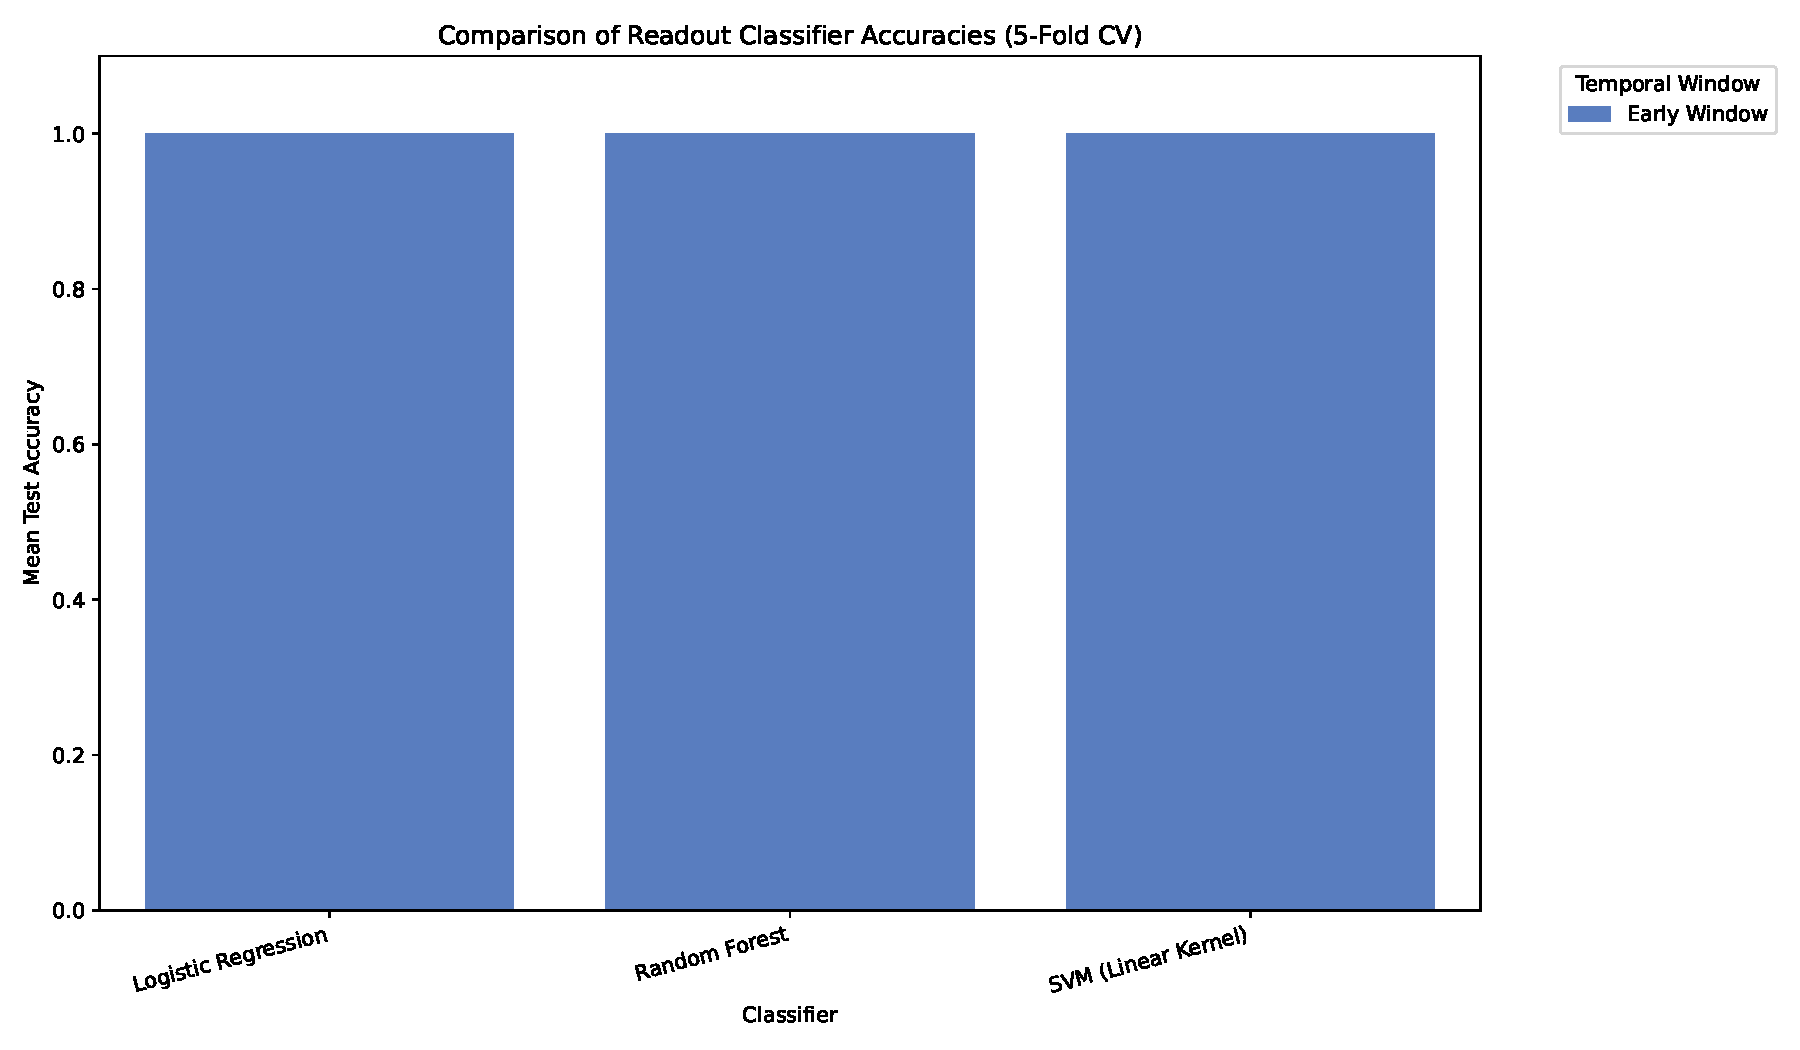
\includegraphics[width=0.8\textwidth]{pictures/chLSM/classifier_accuracy_comparison.pdf}
    \caption{Reported five-fold accuracy for three readouts on duplicated deterministic Early Window features. All classify the two unique feature vectors without error; the zero variance is not an independent generalization estimate.}
    \label{fig:m4_classifier_accuracy_comparison_actual}
\end{figure}

\begin{figure}[H]
    \centering
    \begin{subfigure}{0.48\textwidth}
        \centering
        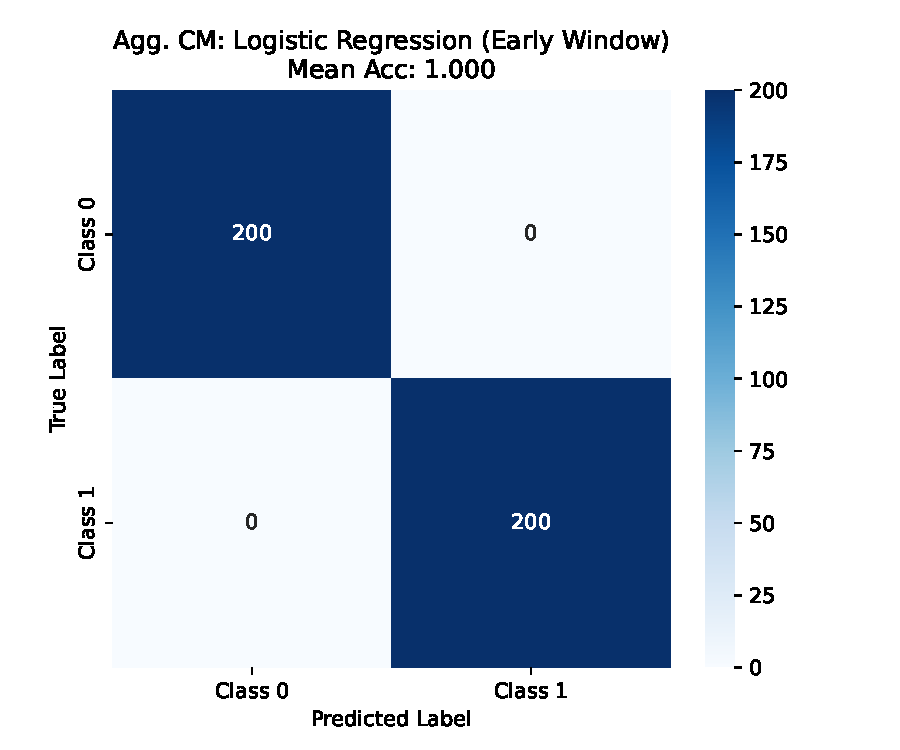
\includegraphics[width=\linewidth]{pictures/chLSM/cm_cv_logistic_regression_win_early_window.pdf}
        \caption{Logistic Regression (Acc: 1.000)}
        \label{fig:m4_cm_logreg_actual}
    \end{subfigure}
    \hfill
    \begin{subfigure}{0.48\textwidth}
        \centering
        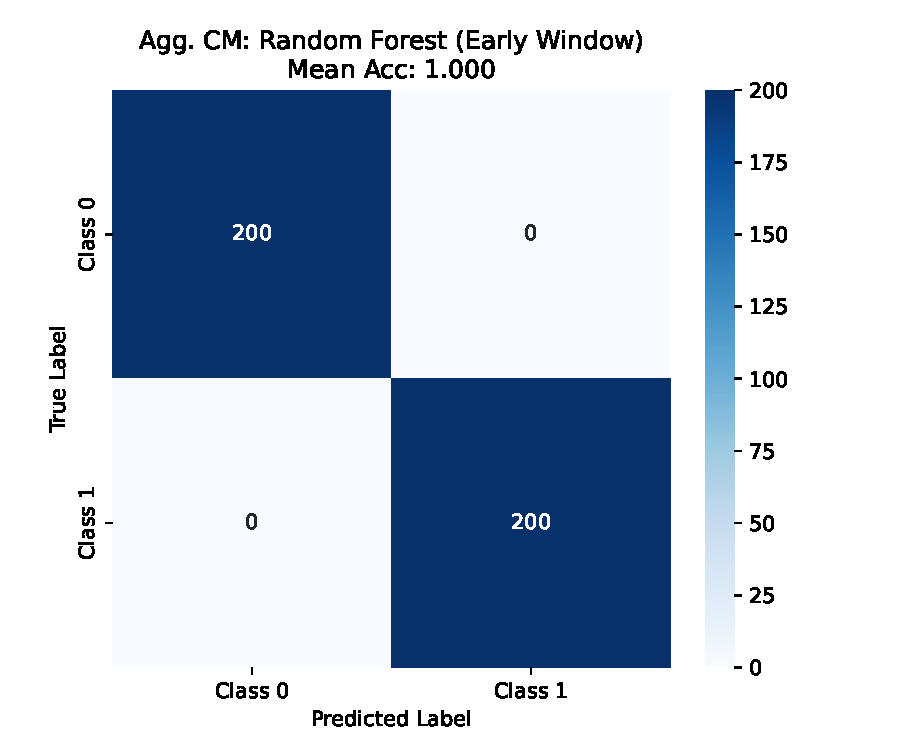
\includegraphics[width=\linewidth]{pictures/chLSM/cm_cv_random_forest_win_early_window.pdf}
        \caption{Random Forest (Acc: 1.000)}
        \label{fig:m4_cm_rf_actual}
    \end{subfigure}
    \vspace{1em}
    \begin{subfigure}{0.48\textwidth}
        \centering
        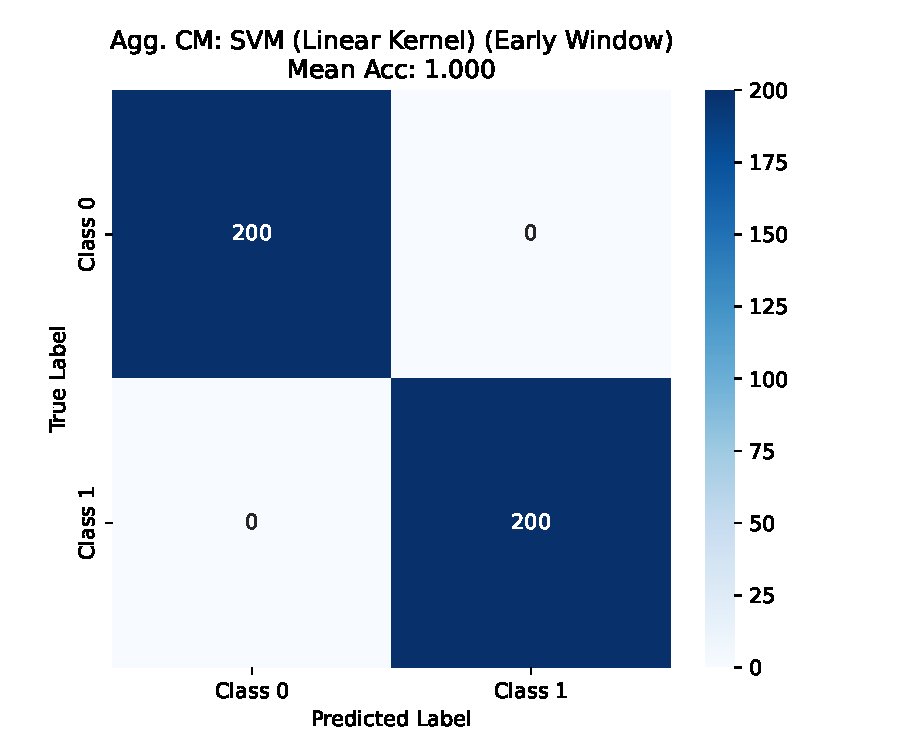
\includegraphics[width=\linewidth]{pictures/chLSM/cm_cv_svm_(linear_kernel)_win_early_window.pdf}
        \caption{SVM, Linear Kernel (Acc: 1.000)}
        \label{fig:m4_cm_svm_linear_actual}
    \end{subfigure}
    \caption{Aggregated five-fold confusion matrices. Counts reflect 200 duplicate copies of each of two unique feature vectors. $\beta=0.05$, $M_{\text{th}}=0.5$.}
    \label{fig:m4_confusion_matrices_all_actual}
\end{figure}

\subsection{Discussion and Significance}
\label{sec:module4_discussion}

\subsubsection{Observed Separability}

The two unique 512-dimensional feature vectors are separable by the fitted linear models, so Random Forest's nonlinear boundary was unnecessary for these stored points. Because the classes differ by a large scalar amplitude before entering the reservoir, the result is best treated as an implementation sanity check.

Mathematically, two finite sets are linearly separable if a hyperplane assigns every observed point to the correct side. The fitted linear models supply evidence of that property for the two stored vectors, but not for an unobserved distribution around them.

\subsubsection{Scope of the Controlled Result}

Three considerations define the scope of this result.

First, the task is a contrast between two constant-amplitude pulses with no additive noise or within-class variation. An energy detector on the raw input would also distinguish them perfectly. No raw-input linear baseline was fitted, so improvement in representation geometry is not established.

Second, a deterministic transformation cannot create label information absent from its input. The observed separability indicates that the selected readout can access the original amplitude contrast after reservoir processing; it does not quantify mutual information or improvement over raw input.

Third, separability of two deterministic pulse responses says little about noisy, heterogeneous EEG observations. The later SHAPE analyses therefore stand on their own and inherit the limitations documented in Chapter~\ref{chap:arspi_net}.

\subsubsection{What This Means for ARSPI-Net}

Within this scope, the result verifies that the implementation produces a nonconstant response that a simple readout can distinguish.

At the representation level, the selected operating point ($\beta=0.05$, $M_{\text{th}}=0.5$) maps the two amplitudes to distinct Early Window firing-rate vectors. Since the original one-dimensional amplitude contrast was already easy, the result does not show that the reservoir performed a harder representational task.

Architecturally, this is sufficient to pass a basic component test before forming channel-level features. It does not determine what a later graph model learns or show that graph propagation isolates inter-electrode relations.

The data-processing inequality remains a useful boundary: this fixed transformation cannot increase mutual information with the label. Any later change in Fisher ratio is a geometric statistic for a chosen representation, not evidence that information was created.


%% ===================================================================
%% CHAPTER SYNTHESIS
%% ===================================================================
\section{Chapter Synthesis: Toward ARSPI-Net Integration}
\label{sec:chapter3_synthesis}

The controlled observations inform, but do not validate, the later architecture. The membrane-decay sweep, threshold comparison, window comparison, and readout check each have an inspectable computational path. That traceability supports implementation auditing; it is not equivalent to a causal explanation of every population response, nor does it establish Koopman linearization, the Echo State Property, or clinical interpretability.

\subsection{Convergent Design Specifications}
\label{sec:design_specifications}

The experimental investigations across Modules~1--4 support the following provisional design conclusions:

\begin{enumerate}
    \item \textbf{Temporal control} (Module~1): $\beta=0.05$ gives intermediate persistence for the pulse and epoch tested here. It is carried forward as a provisional setting.

    \item \textbf{Response regime} (Module~2): $M_{\text{th}}=0.5$ produces amplitude-dependent spikes in the one tested realization. Stability relative to the high-threshold condition was not tested with matched seeds.

    \item \textbf{Window sensitivity} (Module~3): For the two deterministic responses, Early Window mean rates are separable and Late Window mean rates are not. Duplicate rows prevent a generalization claim.

    \item \textbf{Readout check} (Module~4): Linear readouts separate the two unique Early Window response vectors. The raw amplitude contrast is already separable, so no improvement over input space is established.
\end{enumerate}

\subsection{Operating Point Specification}
\label{sec:validated_configuration}

Table~\ref{tab:ch3_config} records the provisional configuration used to connect this characterization to Chapter~\ref{chap:embeddings}. That chapter separately evaluates 256 neurons, steps 10--70, and six-bin spike counts reduced to 64 dimensions.

\begin{table}[htbp]
\centering
\small
\caption{Provisional operating point from controlled characterization and later separately evaluated refinements.}
\label{tab:ch3_config}
\renewcommand{\arraystretch}{1.2}
\begin{tabularx}{\textwidth}{|>{\raggedright\arraybackslash}p{3.5cm}|>{\centering\arraybackslash}p{2.5cm}|>{\raggedright\arraybackslash}X|}
\hline
\textbf{Parameter} & \textbf{Value} & \textbf{Rationale} \\
\hline
Membrane decay ($\beta$) & 0.05 & Balances persistence and responsiveness; $\tau_m \approx 20$ steps (Module~1) \\
\hline
Firing threshold ($M_{\text{th}}$) & 0.5 & Produced graded spikes in one tested realization (Module~2) \\
\hline
Feature window & Steps 20--50 & Concentration of mean-rate discriminative content (Module~3) \\
\hline
Reservoir size & 512 neurons & Characterization configuration; 256 evaluated separately in Chapter~\ref{chap:embeddings} \\
\hline
Feature type & Mean firing rates & Baseline representation; refined to BSC$_6$ in Chapter~\ref{chap:embeddings} \\
\hline
Readout & Linear classifier & Separates the two unique controlled response vectors (Module~4) \\
\hline
\end{tabularx}
\end{table}

The readout result confirms only that the two stored response vectors are distinct in a linearly accessible way. The richer BSC$_6$ representation in Chapter~\ref{chap:embeddings} is motivated by the desire to preserve within-window timing, not by proof that this experiment improved the original geometry.

\subsection{Implications for the Dissertation}
\label{sec:ch3_implications}

The four modules provide component checks under controlled stimulation. Their implications are design hypotheses to be re-evaluated in later analyses.

\subsubsection{Architectural Implications}

Spike-based operation was retained because it supplies the event counts used by the downstream representation. The study did not establish a cross-seed robustness hierarchy, and the deterministic separability check does not determine what the later graph model learns.

\subsubsection{Methodological Implications}

The window comparison motivates testing temporally resolved counts rather than relying only on one mean rate. It does not show that later bins contain recoverable information; that would require a noisy, independently sampled task and a corresponding readout comparison.

No EEG window is inferred from the synthetic result alone. Chapter~\ref{chap:arspi_net} documents the window used for the available SHAPE summaries and treats the synthetic exercise as background rather than validation.

\subsubsection{Theoretical Implications}

Chapter~\ref{chap:dynamics} computes descriptive statistics of driven reservoir trajectories. Those statistics summarize the implemented transformation; they are not biomarkers, and this chapter does not prove the Echo State Property. The analysis window remains an explicit design choice whose consequences should be checked rather than inferred from thresholding alone.

Chapter~\ref{chap:synthesis} later compares dynamical and graph-derived summaries. The present chapter supplies implementation context for that comparison but does not establish that either summary has physiological meaning.

\subsection{Forward-Looking Design Principles}

The controlled characterization yields five limited design notes:
\begin{itemize}
    \item The selected low threshold produces the spike events required by the embedding pipeline; matched-seed robustness remains untested.
    \item Temporal windowing materially changes the chosen mean-rate readout and should be reported as part of the model specification.
    \item The two deterministic Early Window responses are linearly separable, but improvement over raw input is not established.
    \item Fixed weights and explicit update equations make the computational path inspectable. This is traceability, not a guarantee that each output has a unique physiological interpretation.
    \item The synthetic operating point is carried forward provisionally; the SHAPE results do not retroactively validate the simplified pulse experiments.
\end{itemize}

In summary, the chapter records how one fixed-weight reservoir implementation responds to controlled pulses and explains why $\beta=0.05$ and $M_{\text{th}}=0.5$ were carried forward. Unlike adaptive-reservoir approaches such as NeuCube \cite{kasabov_neucube_2014}, the realized weights here remain fixed after initialization. That choice makes the implemented transformation reproducible when the seed, weights, update rule, and preprocessing are retained, but it does not make the transformation completely interpretable or physiologically identified. Chapter~\ref{chap:embeddings} next evaluates compact temporal encodings for the downstream analyses.

\newpage
\chapter{From Spike Trains to Node Embeddings: A Reservoir-to-Graph Representation Pipeline}
\label{chap:embeddings}

\section{Introduction: From Reservoir Output to Fixed-Length Features}
\label{sec:ch4_intro}

Given the provisional operating point from Chapter~\ref{chap:lsm}, this chapter compares ways to convert a sparse spike matrix into a fixed-length vector. The comparison asks how mean rate, latency, and binned counts behave on a controlled temporal-pattern task, and how much dimensionality can be removed without a large loss in readout accuracy. A bin index has explicit temporal meaning; a principal component, by contrast, is a data-dependent linear combination and requires more cautious interpretation.

Many spike-train summaries are available, but there is no single representation that is optimal for every task. Here the purpose is narrower: specify one reproducible feature pipeline, compare it with plausible alternatives on synthetic data, and disclose what the comparison does and does not establish for the later graph analysis.

Chapter~\ref{chap:lsm} showed amplitude-dependent spikes in one selected realization and a window-dependent mean-rate contrast for two deterministic pulse responses. This chapter uses a separate, noisy synthetic task with timing and amplitude jitter to make the feature comparison less trivial.

For the synthetic experiments and the audited rerun specification, one channel produces a binary spike matrix $\mathbf{S} \in \{0, 1\}^{N_{\text{res}} \times T}$ with $N_{\text{res}}=256$ units and $T=60$ steps from the early window (steps 10--70). This is a 15,360-element object indexed by unit and time. A graph readout requires a fixed-length vector $\mathbf{h}_v^{(0)} \in \mathbb{R}^d$ for each node. The summary from $\mathbf{S}$ to $\mathbf{h}_v^{(0)}$ determines which temporal distinctions remain available to that readout.


\section{Background: Neural Coding}
\label{sec:neural_coding_theory}

The question of how to extract a feature vector from a spike train is a specific instance of the \emph{neural coding problem}, one of the foundational questions in computational neuroscience. The debate concerns what aspects of a neural spike train carry information about the stimulus: the overall firing rate (rate coding), the precise timing of individual spikes (temporal coding), or some combination \cite{gerstner_spiking_2002, dayan2001, Rieke1997}.

This distinction is relevant to the feature comparison: if mean firing rate supports the selected readout, finer bins may be unnecessary for this task; if binned counts perform better, the ordering of activity within the window is useful to that readout.

The data-processing inequality states that a deterministic summary cannot increase mutual information with the label. No mutual information or statistical sufficiency is estimated here. Cross-validated readout accuracy is instead used as a task-specific measure of accessibility, and retained PCA variance is reported as a separate compression summary.

\subsection{An Evaluation Task: Temporal Pattern Discrimination}

The controlled task presents three sub-pulses with strong--medium--weak amplitudes for Class~0 and the reverse order for Class~1. The nominal profiles contain the same set of amplitudes, but independent amplitude and timing jitter plus additive Gaussian noise mean that realized trial energy is not exactly matched. The executable configuration uses noise standard deviation 0.5, amplitude jitter of $\pm30\%$, timing jitter of $\pm5$ steps, 200 generated observations per class, and random seed 42. Consequently, performance differences are evidence about these feature/readout combinations on this generator, not proof that only temporal order distinguishes every realized observation.


\section{Reservoir Size Ablation}
\label{sec:size_ablation}

Reservoir size changes both feature dimension and computational cost. The BSC$_6$--PCA-64--logistic pipeline was evaluated for $N_{\text{res}}\in\{64,128,256,512\}$ using five fixed stratified splits. Scaling and PCA were fitted only on each training fold and applied to its held-out fold.

The fold accuracies are shown in Figure~\ref{fig:reservoir_size_ablation}. The differences are small for this synthetic generator. No valid hypothesis test was performed on the five correlated fold scores, so the result is used to select 256 units as a cost--accuracy compromise rather than to claim statistical equivalence or a universal saturation point.

\begin{figure}[H]
    \centering
    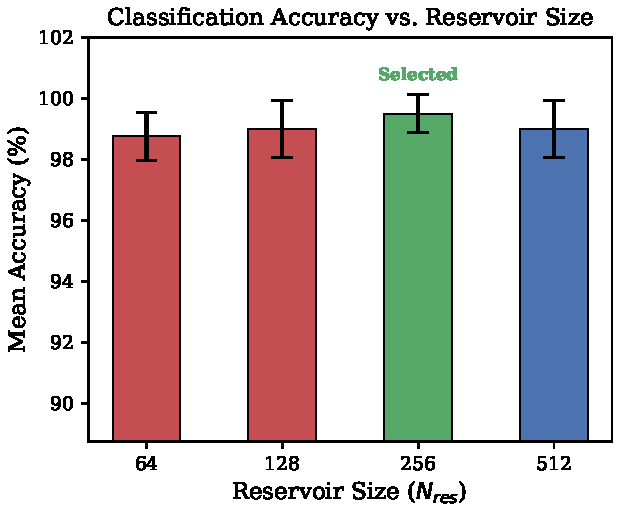
\includegraphics[width=0.65\textwidth]{pictures/chLSMEmbeddings/ablation_reservoir_size.pdf}
    \caption{Mean held-out-fold accuracy versus reservoir size. Scaling and PCA were fitted within each training fold; error bars are the standard deviation across five correlated folds and are not confidence intervals.}
    \label{fig:reservoir_size_ablation}
\end{figure}


\section{Descriptive Comparison of Representation Geometry}
\label{sec:separability}

\subsection{Fisher Discriminant Ratio with Regularization}

The Fisher Discriminant Ratio (FDR $=\operatorname{tr}(\mathbf{S}_W^{-1}\mathbf{S}_B)$) summarizes between-class relative to within-class scatter \cite{duda_pattern_2001}. For the 1536-dimensional BSC$_6$ vectors with 200 samples per class, $\mathbf{S}_W$ is rank-deficient (rank $\leq398<1536$). Tikhonov regularization was applied as $\mathbf{S}_W\leftarrow\mathbf{S}_W+\epsilon\mathbf{I}$ with $\epsilon=10^{-4}\operatorname{tr}(\mathbf{S}_W)/d$. The same rule was used for each representation, but differing dimensions and spectra still limit direct ratio comparisons.

\subsection{Results and Limits of the FDR Comparison}

The regularized FDR comparison in Figure~\ref{fig:fdr_comparison} gives the following descriptive values:
\begin{itemize}
    \item Raw input (binned): FDR = 0.13
    \item Linear filter (5-point moving average + binning): FDR = 0.13
    \item LSM reservoir (BSC$_6$): FDR = 1158
\end{itemize}

The numerical ratio is approximately $8{,}900$, but it should not be interpreted as an effect-size ratio or a causal decomposition. The representations have different dimensions and covariance spectra, and the regularized inverse is sensitive to the chosen $\epsilon$ in this rank-deficient setting. Moreover, a single moving-average baseline does not isolate thresholding, recurrence, and expansion. The comparison shows that this particular regularized statistic is much larger for BSC$_6$ than for the two stated baselines; it does not show which reservoir mechanism caused the difference.

\begin{figure}[H]
    \centering
    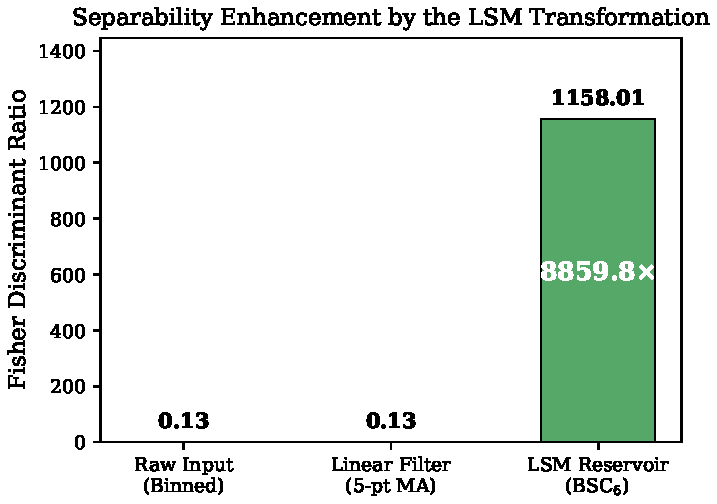
\includegraphics[width=0.7\textwidth]{pictures/chLSMEmbeddings/fdr_three_way_comparison.pdf}
    \caption{Regularized Fisher ratio for raw binned input, a five-point moving-average baseline, and BSC$_6$. Values are descriptive and are sensitive to dimension, covariance rank, and the regularization rule; they do not identify a causal contribution of reservoir components.}
    \label{fig:fdr_comparison}
\end{figure}


\section{Comparative Analysis of Neural Coding Representations}
\label{sec:coding_comparison}

\subsection{Design and Results}

Four coding schemes were compared, each evaluated with both logistic regression and SVM-RBF classifiers (Table~\ref{tab:coding_results}, Figure~\ref{fig:coding_comparison}).

\begin{table}[H]
    \centering
    \caption{Mean held-out-fold accuracy (\%) for each coding scheme on the synthetic temporal-pattern generator. Preprocessing was fitted within each training fold. Error terms are fold standard deviations, not confidence intervals.}
    \label{tab:coding_results}
    \begin{tabular}{|l|c|c|}
        \hline
        \textbf{Coding Scheme} & \textbf{Logistic Regression} & \textbf{SVM (RBF)} \\
        \hline
        Mean Firing Rate (MFR) & $47.5\% \pm 4.1\%$ & $51.2\% \pm 4.9\%$ \\
        Latency to First Spike (LFS) & $70.0\% \pm 4.4\%$ & $70.8\% \pm 3.3\%$ \\
        BSC (3 Bins) & $98.3\% \pm 1.3\%$ & $98.3\% \pm 1.3\%$ \\
        \textbf{BSC (6 Bins)} & $\mathbf{99.5\% \pm 0.6\%}$ & $\mathbf{99.5\% \pm 0.6\%}$ \\
        \hline
    \end{tabular}
\end{table}

\begin{figure}[H]
    \centering
    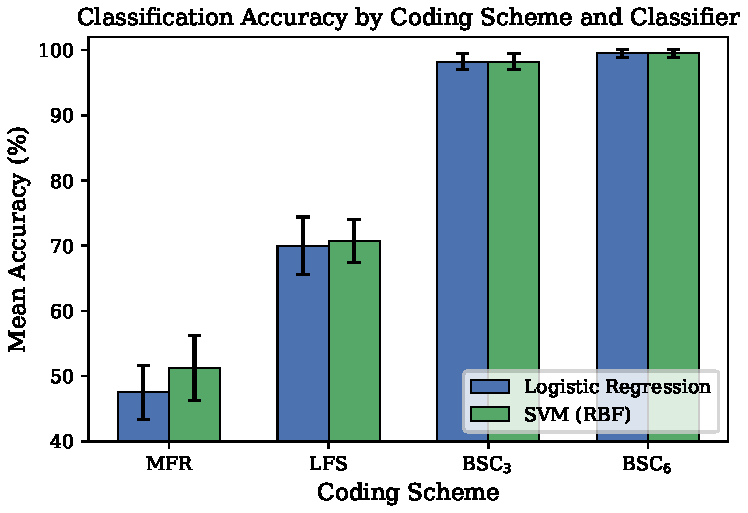
\includegraphics[width=0.65\textwidth]{pictures/chLSMEmbeddings/coding_scheme_accuracy_comparison.pdf}
    \caption{Held-out-fold accuracy by coding scheme and classifier. BSC$_6$ performs substantially better than MFR on this generator, showing that within-window binning is useful to these readouts; it does not establish that all label information is exclusively temporal.}
    \label{fig:coding_comparison}
\end{figure}

An additional comparison with inter-spike interval histograms and the Victor--Purpura distance \cite{victor_purpura_1996} reported 99.7\% accuracy at more than 50 times the measured computation. Because performance is near the ceiling and timing depends on the implementation and hardware, this is a practical comparison for the recorded experiment rather than proof of an optimal code.

\subsection{Interpretation of the Coding Comparison}

The MFR logistic-regression result is close to chance for this balanced generator. It indicates that the selected linear readout could not use mean-rate features reliably under these splits. It does not establish zero mutual information, and the realized noisy stimuli are not exactly energy matched.

The BSC$_6$ result shows that six 10-step counts make the generated early-versus-late pattern highly accessible to both selected readouts. Relative to MFR, the representation retains coarse ordering within the 60-step window. The comparison does not exclude contributions from realized amplitude, timing, or noise differences.

First-spike latency gives intermediate accuracy. This is consistent with sensitivity to early timing while discarding later events, although the experiment does not isolate the exact source of its errors.

The large accuracy gap supports BSC$_6$ for the subsequent pipeline. Its magnitude is specific to this generator and should not be projected onto SHAPE EEG without a direct, fold-safe comparison there.

Each BSC$_6$ feature has an explicit neuron and 10-step-bin index, whereas mean rate collapses the full window. This makes the pre-PCA code temporally traceable. Once PCA mixes neurons and bins, that one-to-one feature interpretation no longer holds.


\section{Dimensionality Reduction, Representational Geometry, and Robustness}
\label{sec:pca_robustness}

\subsection{PCA Compression}

PCA was applied to the 1536-dimensional BSC$_6$ vectors. The full-data eigenspectrum is shown descriptively in Figure~\ref{fig:pca_variance}: 64 components account for 50.5\% of total sample variance. For every accuracy estimate, standardization and PCA were refitted inside each training fold before transforming the held-out fold. With that procedure, PCA-64 retained $99.5\%\pm0.6\%$ accuracy, and PCA-5 also yielded $99.5\%\pm0.6\%$ on this generator. These near-ceiling values show that five training-fold principal components were sufficient for the selected readout; they do not prove a unique intrinsic dimension.

PCA is unsupervised, so explained variance alone does not identify class-discriminating directions. The combination of a long eigenspectrum tail and high fold-safe accuracy after compression supports PCA as a practical size reduction for this synthetic dataset. It does not establish that discarded variance is nuisance, and there is no biological variability in the generator.

\begin{figure}[H]
    \centering
    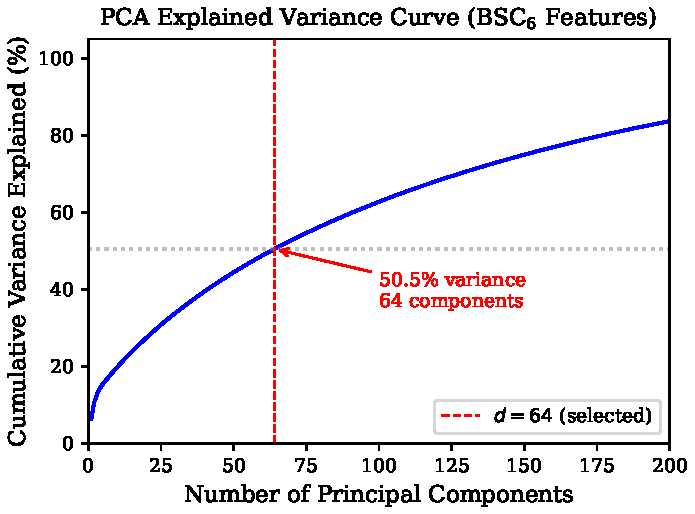
\includegraphics[width=0.65\textwidth]{pictures/chLSMEmbeddings/pca_explained_variance.pdf}
    \caption{Full-sample cumulative explained variance for BSC$_6$. Accuracy at each component count was evaluated separately with fold-fitted PCA; five components were sufficient for near-ceiling readout accuracy on this generator.}
    \label{fig:pca_variance}
\end{figure}

\subsection{Interpretation of Principal Component Structure}

Figure~\ref{fig:pca_components} averages each full-data component's signed loadings across neurons within each of the six bins. The display is an exploratory temporal summary: PCA signs are arbitrary, averaging can hide heterogeneous neuron loadings, and no supervised statistic establishes that a particular component is a primary class discriminator.

The profiles show that the leading components mix contributions from several time bins. They may help inspect the compression globally, but individual PCA coordinates should not be assigned fixed semantic labels such as onset or relative timing without stability and loading-level analyses. The downstream model receives numerical coordinates, not guaranteed disentangled concepts.

\begin{figure}[H]
    \centering
    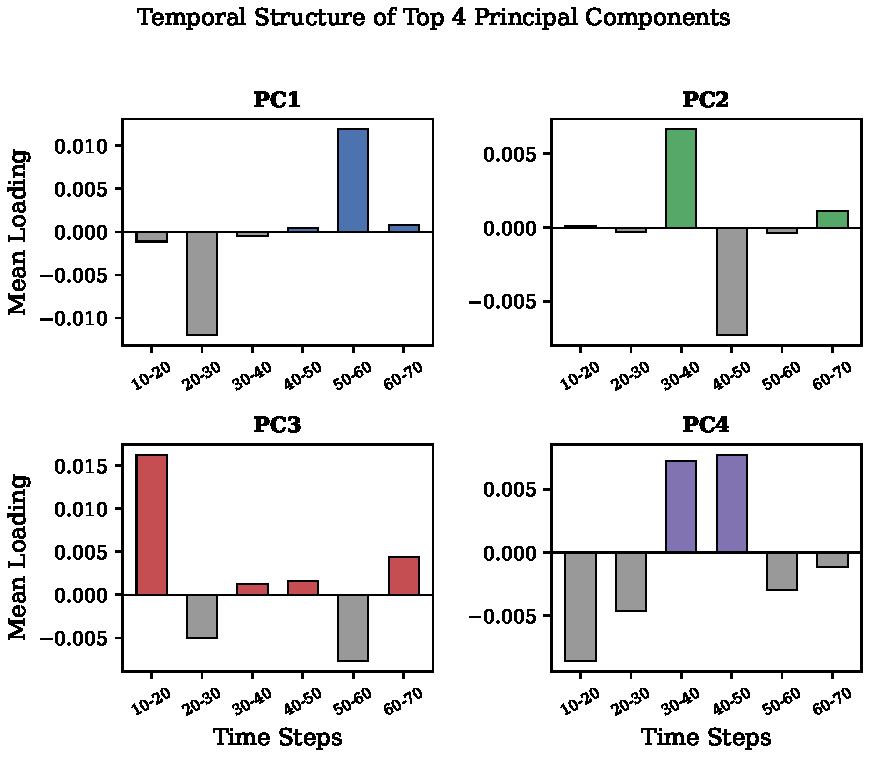
\includegraphics[width=0.9\textwidth]{pictures/chLSMEmbeddings/pca_component_visualization.pdf}
    \caption{Exploratory temporal profiles of the top four full-data principal components, computed by averaging signed loadings across neurons within each bin. Component signs are arbitrary and the averages do not provide functional labels.}
    \label{fig:pca_components}
\end{figure}

\subsection{Cross-Initialization Robustness}

Across 10 reservoir initializations, BSC$_6$+PCA-64 yielded mean fold-averaged accuracy of $99.3\%\pm0.3\%$ across seeds, while MFR yielded $50.8\%\pm2.7\%$ (Figure~\ref{fig:robustness}). PCA and scaling were fitted within each training fold. The reported standard deviations describe variation across these 10 seeds, not uncertainty for an unrestricted population of reservoirs.

The seed sweep shows stable task accuracy for the synthetic generator. It does \emph{not} show that independently initialized reservoirs or independently fitted PCA bases produce coordinate-wise comparable node features. That distinction matters for graph inputs and motivates the common, fold-fitted basis specified in the corrected Chapter~\ref{chap:arspi_net} analysis code.

\begin{figure}[H]
    \centering
    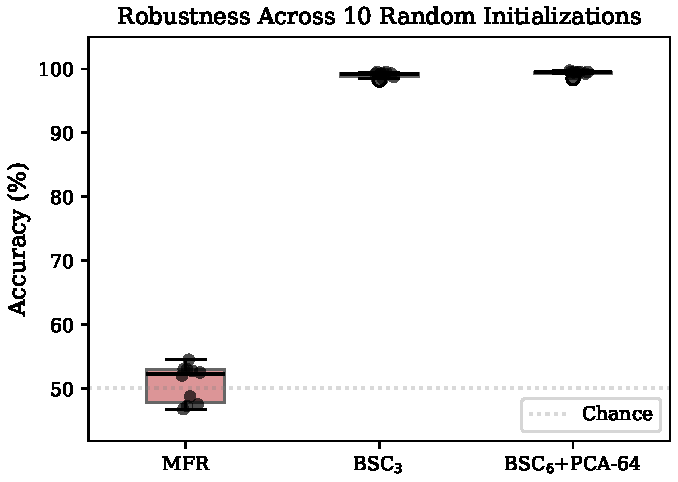
\includegraphics[width=0.55\textwidth]{pictures/chLSMEmbeddings/cross_initialization_robustness.pdf}
    \caption{Fold-averaged accuracy across 10 reservoir initializations. Each dot is one seed; transforms were fitted inside each training fold. Stability of accuracy does not imply alignment of feature coordinates across seeds.}
    \label{fig:robustness}
\end{figure}

\subsection{Parameter Sensitivity}

The pipeline was also evaluated over the finite grid $\beta\in\{0.03,\ldots,0.08\}$ and $M_{\text{th}}\in\{0.3,\ldots,0.7\}$ (Figure~\ref{fig:sensitivity}), with fold-fitted preprocessing. High accuracy throughout this grid shows low sensitivity for the synthetic generator and sampled values; it does not validate transfer to different input statistics.

\begin{figure}[H]
    \centering
    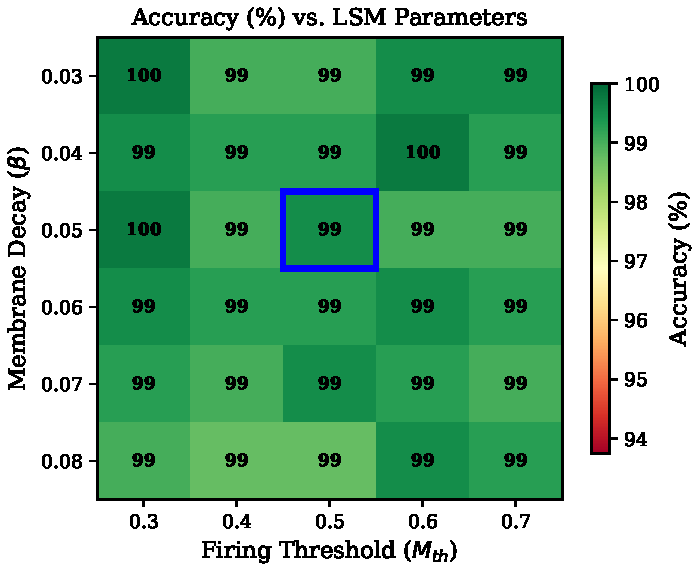
\includegraphics[width=0.6\textwidth]{pictures/chLSMEmbeddings/parameter_sensitivity_heatmap.pdf}
    \caption{BSC$_6$+PCA-64 held-out-fold accuracy across the sampled $\beta$ and threshold grid. Results describe this generator and finite grid only.}
    \label{fig:sensitivity}
\end{figure}


\section{Chapter Synthesis: Provisional Embedding Specification}
\label{sec:ch4_synthesis}

\subsection{Summary of Findings}

The synthetic experiments support the following limited conclusions:

\begin{enumerate}
    \item \textbf{Representation geometry differs}: The regularized FDR is much larger for BSC$_6$ than for the raw and moving-average baselines. Dimension, covariance, and regularization prevent a causal or effect-size interpretation of the $8{,}900\times$ numerical ratio.

    \item \textbf{Coarse temporal binning helps on this task}: BSC$_6$ substantially outperforms MFR for the noisy early-versus-late generator. Each pre-PCA bin maps to a specified response interval, but no mutual-information claim follows.

    \item \textbf{Fold-fitted compression preserves synthetic-task accuracy}: PCA-64 retains near-ceiling accuracy when fitted inside each training fold. PCA coordinates mix bins and neurons and therefore do not preserve a one-feature/one-window interpretation.

    \item \textbf{Accuracy is stable over the tested settings}: BSC$_6$+PCA-64 yields $99.3\%\pm0.3\%$ across 10 seeds and high accuracy over the sampled parameter grid. This does not establish coordinate alignment or real-data robustness.
\end{enumerate}

\subsection{Final Embedding Specification}

\begin{table}[H]
    \centering
    \caption{Audited specification for a corrected real-data rerun. PCA must be fitted on training data only and shared across channels when coordinates are compared.}
    \label{tab:final_embedding_spec}
    \renewcommand{\arraystretch}{1.2}
    \begin{tabular}{|l|p{8cm}|}
        \hline
        \textbf{Parameter} & \textbf{Specification} \\
        \hline
        Reservoir size ($N_{\text{res}}$) & 256 neurons \\
        Membrane decay ($\beta$) & 0.05 \\
        Firing threshold ($M_{\text{th}}$) & 0.5 \\
        Feature window & Time steps 10--70 post-stimulus \\
        Coding scheme & BSC$_6$ (6 bins $\times$ 10 steps each) \\
        Dimensionality reduction & PCA, 64 components \\
        Evaluation rule & Fit scaling and one common PCA basis on each training fold only; transform held-out data without refitting \\
        \textbf{Output} & $\mathbf{h}_v^{(0)} \in \mathbb{R}^{64}$ per channel index \\
        \hline
    \end{tabular}
\end{table}

\subsection{Scope and Transfer Considerations}

The pipeline was selected on synthetic stimuli. The audit found three mismatches in the archived SHAPE workflow. PCA was fitted globally and, in some scripts, separately by channel. The primary Chapter~5 extractor divided the full 256-sample post-stimulus epoch into six 42-sample bins and dropped the final four samples, rather than using steps 10--70; the later temporal-traceability analysis did use the early window. Finally, the primary script initialized different random reservoir weights for each channel. Equal-numbered neuron features therefore did not share a common transformation across graph nodes. Thus the primary Chapter~5 embedding and the early-window attention analysis are different representations despite sharing the BSC$_6$ label, and the archived node coordinates were misaligned before PCA.

The corrected source applies one saved reservoir to every channel, uses steps 10--70, standardizes on the training fold, and fits one common PCA basis inside that fold. Raw SHAPE inputs were not included in the audited source package, so this corrected real-data analysis could not be rerun. Archived numerical results remain descriptive and do not validate the specification in Table~\ref{tab:final_embedding_spec}.

\subsection{Exploratory Temporal Traceability Check}
\label{sec:ch4_temporal_traceability}

Temporal traceability is used here in a narrow operational sense: every uncompressed BSC$_6$ value has a known response interval. The following archived profile correlations are exploratory comparisons with conventional ERP summaries, not validation that an early spike bin measures an ERP component.

Per-channel means were formed for six early intervals (39--78, 78--117, 117--156, 156--195, 195--234, and 234--273~ms) from the archived centered summaries ($N=211$ subjects; 633 subject--condition observations). The archived profile analysis reported $r=0.65$ against a P300 summary (250--500~ms) and $|r|=0.82$ against an LPP summary (500--800~ms), with a largest channel-wise value of $r=0.837$ for Channel~31. These correlations compare aggregate profiles; they are not subject-level recovery statistics. The BSC intervals overlap only the beginning of the stated P300 window and do not overlap the LPP window, so the associations cannot establish direct temporal correspondence with either full component.

The values show covariation among aggregate summaries that may share condition or channel structure. They do not show that early bins recover the P300 or LPP, do not provide a patient-level $R^2$, and do not establish clinical utility \cite{nelson_hajcak_2017}.

An archived temporal-resolution sweep reported:
\begin{center}
\begin{tabular}{lcccc}
\toprule
\textbf{Bins} & \textbf{Resolution} & \textbf{Accuracy} & \textbf{Peak Bin} & \textbf{Peak Acc.} \\
\midrule
6 & 39.1~ms & $67.0\% \pm 5.4\%$ & Bin 6 (234--273~ms) & $68.1\%$ \\
12 & 19.5~ms & $65.9\% \pm 3.3\%$ & Bin 10 (176--195~ms) & $66.8\%$ \\
24 & 7.8~ms & $63.5\% \pm 5.5\%$ & Bin 23 (172--180~ms) & $64.3\%$ \\
\bottomrule
\end{tabular}
\end{center}
Accuracy was lower at finer resolutions in this finite sweep. Because only three resolutions were tested and no information-bottleneck quantity was estimated, the result does not identify a compression--relevance frontier or an optimal resolution \cite{tishby_deep_2015}.

The archived PCA-64 features yielded negative out-of-sample $R^2$ values (no improvement over a mean-prediction baseline) for the reported ERP-scalar regressions and 33.3\% three-class accuracy after subject centering. A principal-angle calculation returned zero-degree angles in the tested PCA coordinate space. Because the original PCA was fitted globally on uncentered data and the compared subspaces may span the same retained ambient coordinates, that angle result does not prove that subject and condition effects are biologically identical or that centering must destroy signal. The corrected analysis requires fold-fitted PCA and cannot be rerun without the raw SHAPE inputs.

The defensible traceability claim is therefore structural: an uncompressed bin maps to a fixed interval by construction. The profile correlations are supplementary descriptors. They are not directly comparable to analyses of learned connectivity, prototype similarity, or post-hoc attribution because those methods answer different questions \cite{kasabov_neucube_2014,doborjeh_explainable_2021,barnett_protopmed_2024}.

\subsection{Place in the Dissertation}

This chapter specifies the per-channel temporal encoding stage. Uncompressed BSC$_6$ features retain explicit bin indices; PCA components are data-dependent mixtures and do not map one-to-one onto functional response phases. The equations and fitted transforms make the computational path auditable, but they do not eliminate the need for post-hoc checks of what a downstream model uses.

Table~\ref{tab:final_embedding_spec} defines the feature extractor for a future corrected rerun. The archived full-epoch Chapter~5 results and the early-window traceability results remain labeled separately. Downstream outputs cannot be assigned physiological meaning solely because their computational ancestry is recorded.

\newpage
\chapter{From Reservoir Embeddings to Graph-Based Analysis of SHAPE EEG}
\label{chap:arspi_net}

\section{Introduction}
\label{sec:ch5_intro}

This chapter examines whether coupling the channel-wise reservoir representations through a graph improves emotion classification and whether descriptive graph summaries are associated with the available clinical variables.

The preceding chapters characterize the Leaky Integrate-and-Fire reservoir under controlled conditions and evaluate binned spike-count features (BSC$_6$). Here, those features are applied to the multichannel SHAPE recordings. The analysis compares non-propagated channel features with several graph operators and separately summarizes the topology of thresholded similarity graphs.

The chapter addresses three questions on the $211$-subject SHAPE dataset: how subject and condition variability appear in the archived embedding space; whether the tested propagation operators improve classification; and what exploratory associations appear between graph summaries and clinical variables. Additional analyses compare three- and four-class labelings and measure the performance of different feature blocks. These analyses are cohort-specific and exploratory; they do not establish clinical phenotypes or diagnostic biomarkers.

The archived results show that subject-to-subject variation is large relative to the condition term in the fitted embedding decomposition, that none of the tested graph operators exceeds the non-propagated comparison, and that clinical-label analyses yield nominal associations that do not support biomarker claims after the relevant multiplicity and permutation checks. The three- and four-class analyses differ in both label granularity and parts of their preprocessing, so their numerical difference is descriptive rather than a controlled test of a regime transition. Feature-block ablations likewise identify measured differences within this cohort but do not establish disorder-specific mechanisms.

The contribution is a documented comparison of graph and non-graph representations, accompanied by explicit limitations on what the archived analyses can support. The results motivate fold-safe evaluation of a common channel basis and independent replication; they do not provide a general theorem about graph propagation or evidence for layer-specific clinical explanations.

The chapter is organized as follows. Sections~\ref{sec:ch5_gnn_theory}--\ref{sec:ch5_dataset} present the theoretical framework and dataset. Section~\ref{sec:ch5_raw_obs} characterizes the data at each pipeline stage. Section~\ref{sec:ch5_classification} presents the classification experiments. Section~\ref{sec:ch5_variance} develops the variance decomposition, subject normalization, and geometric analyses. Section~\ref{sec:ch5_regime} presents the propagation and graph-construction sweeps. Sections~\ref{sec:ch5_interpretability}--\ref{sec:ch5_nonrep} report exploratory associations with clinical variables. Section~\ref{sec:ch5_4class} presents the granularity comparison, and Section~\ref{sec:ch5_ablation} presents the feature-block ablation.


\section{Theoretical Foundations}
\label{sec:ch5_gnn_theory}

\subsection{Graph Representation of Multichannel EEG}

A multichannel EEG recording can be represented as a graph $\mathcal{G} = (\mathcal{V}, \mathcal{E}, \mathbf{X})$, where the node set $\mathcal{V} = \{v_1, \ldots, v_C\}$ corresponds to $C = 34$ channel indices, the edge set $\mathcal{E}$ encodes pairwise feature similarity, and the node feature matrix $\mathbf{X} \in \mathbb{R}^{C \times d}$ collects channel features. The archived analysis thresholded the Pearson correlation between PCA coordinates:
\begin{equation}
    A_{ij} = \mathbf{1}\left[\rho(\mathbf{x}_i, \mathbf{x}_j) \geq \tau_\rho\right],
\end{equation}
where $\tau_\rho$ retains the top $20\%$ of channel pairs, yielding approximately $112$ edges at $20\%$ density.

This construction has several important limitations. The archived implementation fitted PCA to the complete dataset before cross-validation, and some graph calculations used PCA models fitted separately by channel. It also initialized different random reservoir weights for different channels, so equal-numbered spike features were not generated by a shared transformation. The archived node coordinates are therefore neither fully held out nor commensurate across nodes. Their correlations cannot be interpreted as physiological functional connectivity. The corrected analysis applies one saved reservoir to all channels, standardizes on training-fold rows, fits a common PCA basis on those rows, and applies it unchanged to the held-out fold. Because the raw SHAPE EEG is not distributed with this source package, the corrected Chapter~5 pipeline could not be rerun for this document. Channel labels and montage coordinates were also unavailable; all spatial results refer only to channel indices and have no anatomical interpretation.

A consequence of hard thresholding is that the resulting graph is not guaranteed to be connected. In the archived construction, the population-average graph has five connected components and individual graphs range from one to eight. Information cannot propagate between components. The $20\%$ threshold was an analysis choice; the construction sweep reports sensitivity to several alternatives but does not validate the threshold.

\subsection{Message-Passing Neural Networks}

The message-passing framework \cite{Gilmer2017} updates node representations through iterative neighborhood aggregation:
\begin{equation}
    \mathbf{h}_v^{(k+1)} = \psi^{(k)}\!\left(\mathbf{h}_v^{(k)},\; \bigoplus_{u \in \mathcal{N}(v)} \phi^{(k)}\!\left(\mathbf{h}_u^{(k)}, \mathbf{h}_v^{(k)}, \mathbf{e}_{uv}\right)\right).
\end{equation}
Three architectures are evaluated: GCN \cite{Kipf2017} (normalized adjacency aggregation), GIN \cite{Xu2019} (sum aggregation with an MLP and stated expressivity results relative to the Weisfeiler--Lehman test), and EdgeConv \cite{Wang2019HeterogeneousGNN} (edge-feature MLP with max aggregation). For graph-level classification, mean--max pooling produces $\mathbf{z} = [\text{mean}(\mathbf{H}^{(K)}) \| \max(\mathbf{H}^{(K)})]$.

\subsection{Graph-Topological Descriptors}

Beyond classification, the graph admits mathematical descriptors: global efficiency $E_{\text{glob}} = \frac{1}{C(C-1)} \sum_{i \neq j} d_{ij}^{-1}$, mean clustering coefficient $\bar{C}$, degree heterogeneity (coefficient of variation of degrees), and mean edge weight. For disconnected node pairs, $d_{ij} = \infty$ by convention, so $d_{ij}^{-1} = 0$. Path-based values are computed over the full node set rather than only its largest component unless stated otherwise. At the node level, degree centrality, weighted strength, local clustering, and eigenvector centrality support comparisons among unlabeled channel indices; they are not measures of cortical integration or redundancy here.


\section{The SHAPE Dataset: Specification, Validation, and Preprocessing}
\label{sec:ch5_dataset}

\subsection{Study Description}

The Stress, Health, and the Psychophysiology of Emotion (SHAPE) Community study \cite{noauthor_shape_2018} is a transdiagnostic investigation of psychophysiological markers across the full spectrum of psychiatric symptomatology. Participants viewed affective images from the International Affective Picture System (IAPS) \cite{lang_iaps_2008} while EEG was recorded at $1024$~Hz from $34$ electrodes. Three conditions were administered: negative (unpleasant), neutral, and pleasant. Each file is a $1229 \times 34$ matrix of baseline-corrected, trial-averaged microvolt values. In total, $212$ subjects were provided across three data batches ($68$, $68$, and $76$ subjects respectively).

\subsection{Automated Quality Control Protocol}

An eight-check validation protocol was applied to all $636$ files (Table~\ref{tab:qc_results}, Figure~\ref{fig:qc_verification}). All files passed dimensional verification ($1229 \times 34$), numerical integrity (zero NaN/Inf), and baseline verification (mean $|\overline{x}_{\text{BL}}| < 0.01$~\textmu V). Only $92$ of $26{,}575{,}896$ samples ($0.000\%$) exceeded $5$ standard deviations from the channel mean. The flat-channel check identified Subject~$127$ with all $34$ channels flat in the Neutral condition (Figure~\ref{fig:qc_subject127}) and partially flat channels in the other two conditions. Subject~$127$ was excluded.

\begin{table}[t]
\centering
\caption{Automated quality control results ($636$ files). Subject~$127$ excluded for recording anomaly.}
\label{tab:qc_results}
\small
\begin{tabular}{llll}
\hline
\textbf{Check} & \textbf{Criterion} & \textbf{Result} & \textbf{Status} \\
\hline
1.\ Dimensions & Every file $1229 \times 34$ & $636/636$ & PASS \\
2.\ Completeness & $3$ conditions per subject & $212/212$ & PASS \\
3.\ Numerics & Zero NaN, zero Inf & $0$ violations & PASS \\
4.\ Amplitude & Fail $> 500$~\textmu V & Max $= 325.7$ & PASS \\
5.\ Flat channels & Channel std $< 0.01$~\textmu V & Subj.\ 127: $34/34$ flat & WARN \\
6.\ Outliers & Samples $> 5$ SD & $92/26.6\text{M}$ ($0.000\%$) & PASS \\
7.\ Baseline & $|\overline{x}_{\text{BL}}| < 5$~\textmu V & All $< 0.01$~\textmu V & PASS \\
8.\ Clinical match & All subjects in both databases & $212/212$ & PASS \\
\hline
\end{tabular}
\end{table}

\begin{figure}[H]
    \centering
    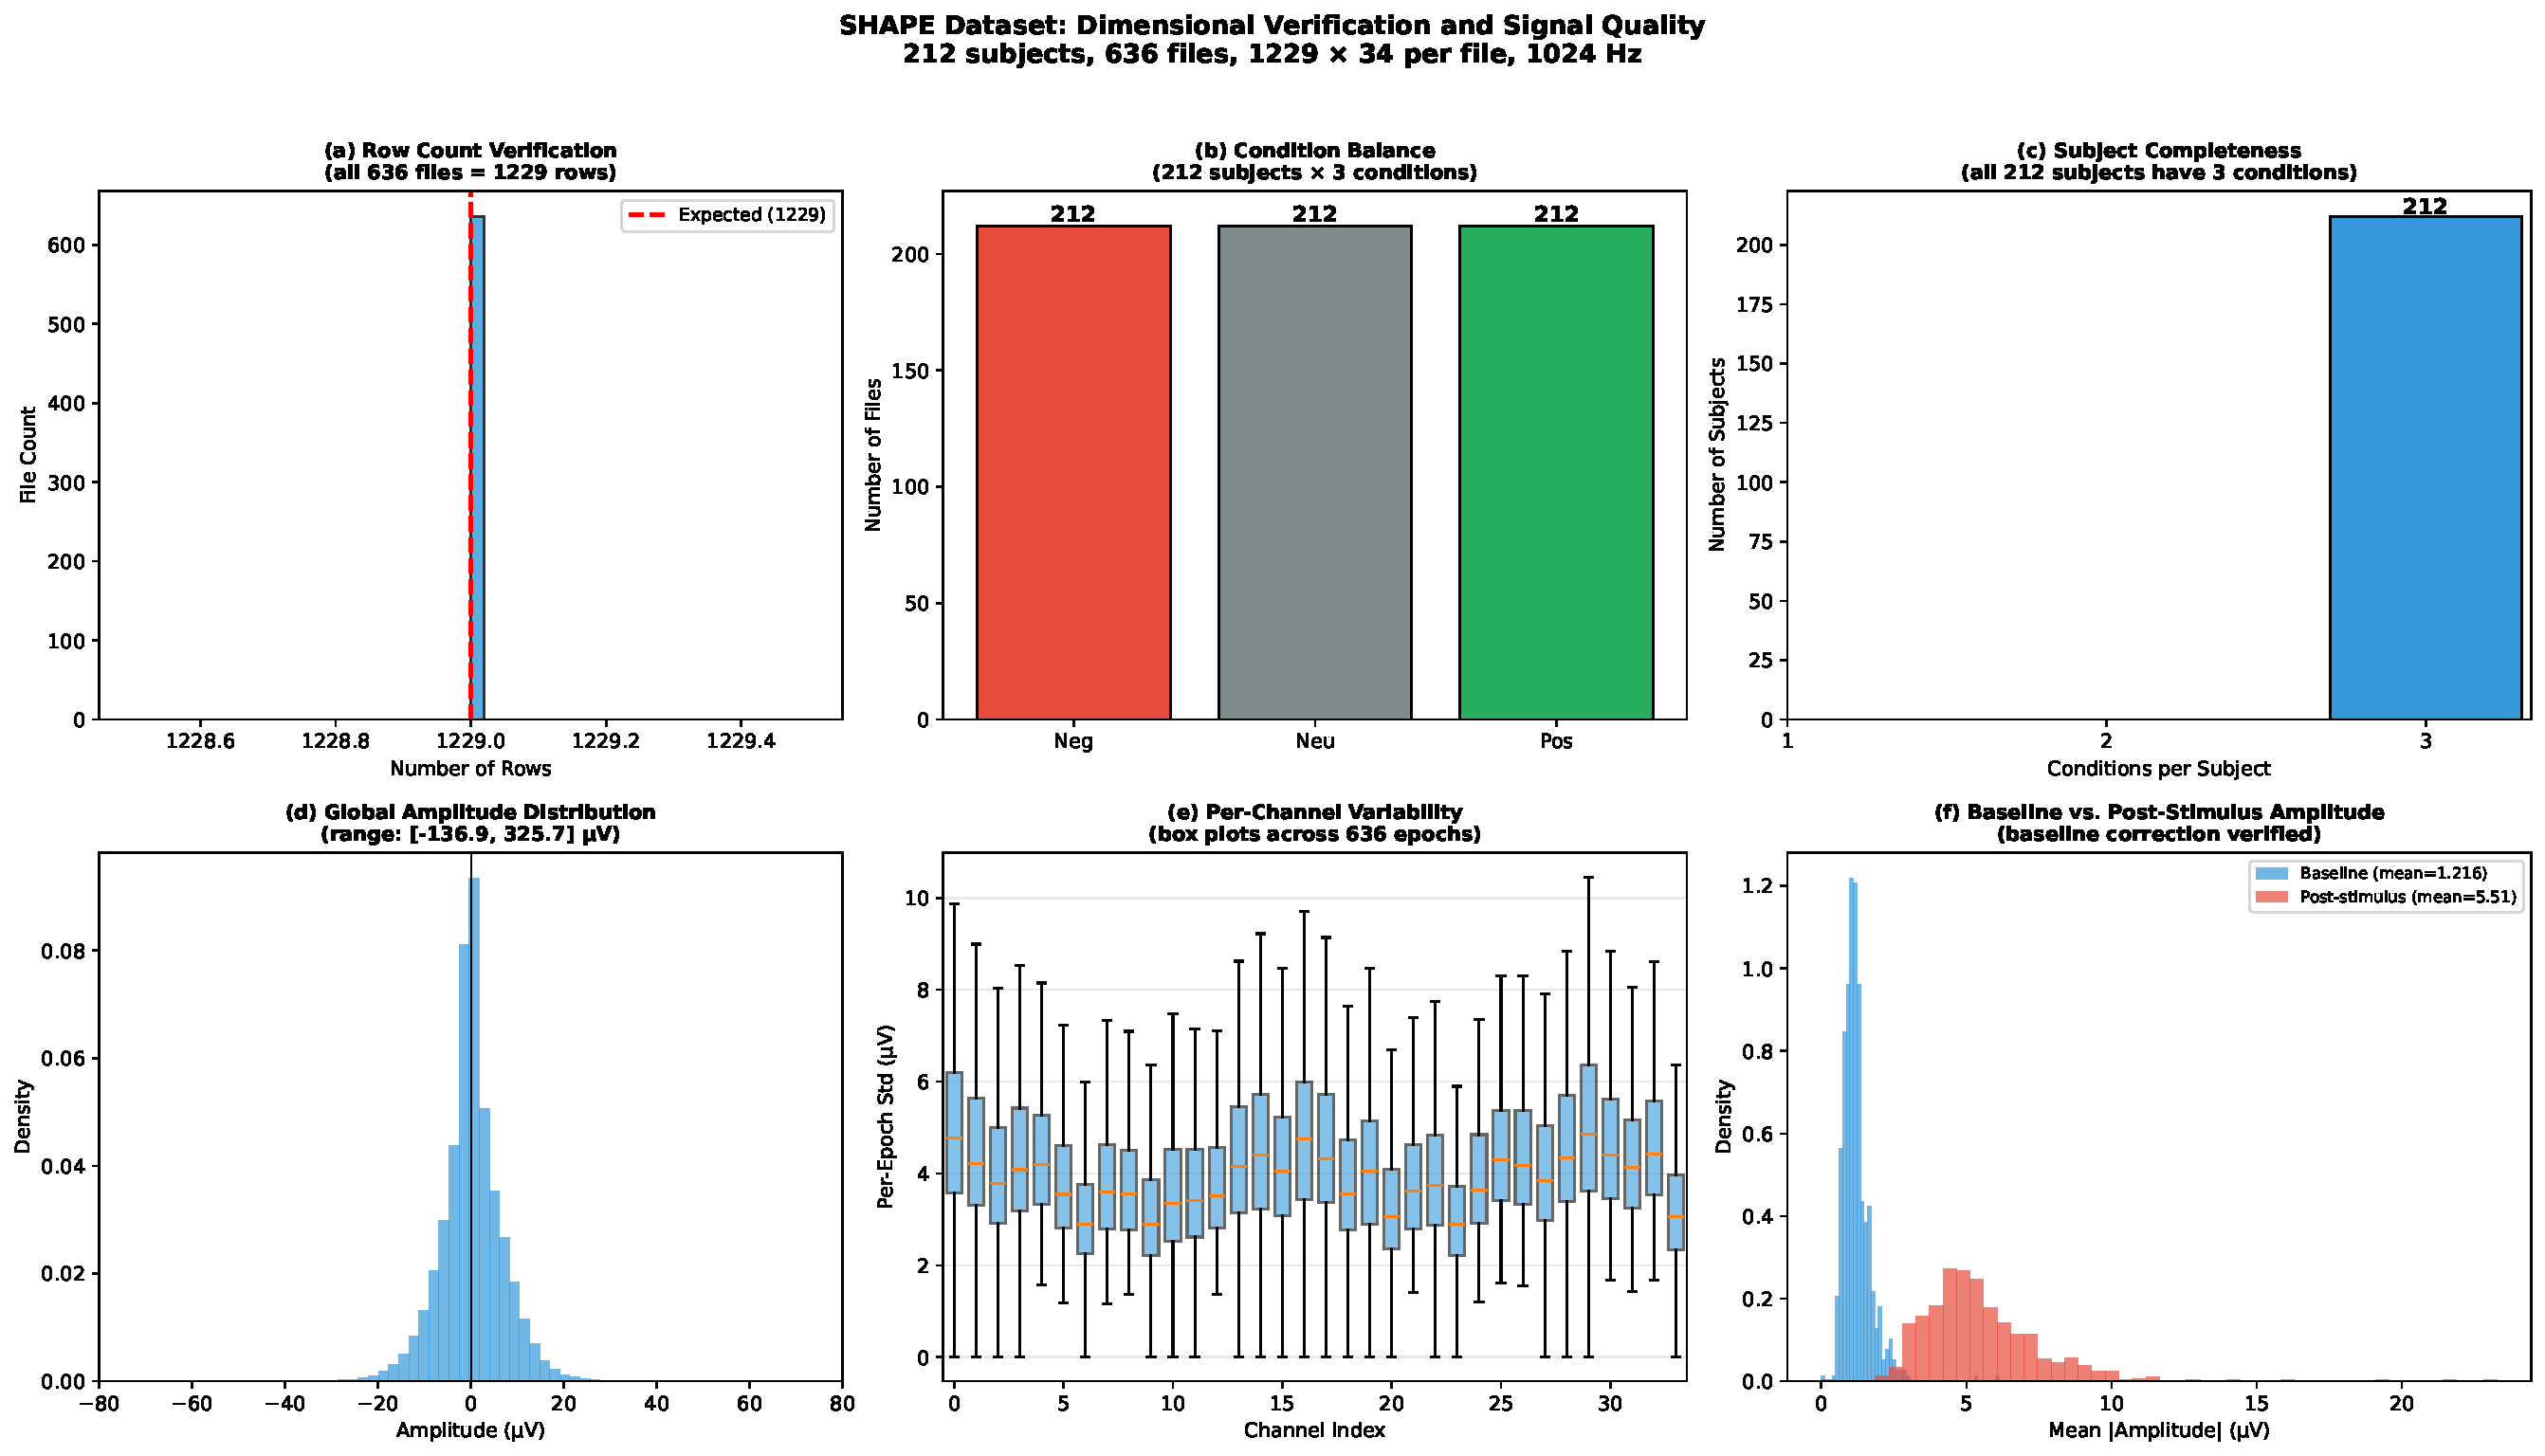
\includegraphics[width=\textwidth]{pictures/chGraphNeuralNetworks/fig_qc_dimensional_verification.pdf}
    \caption{Data verification across $636$ files. (a)~Row counts. (b)~Condition balance. (c)~Subject completeness. (d)~Global amplitude distribution. (e)~Per-channel variability. (f)~Baseline vs.\ post-stimulus amplitude.}
    \label{fig:qc_verification}
\end{figure}

\begin{figure}[H]
    \centering
    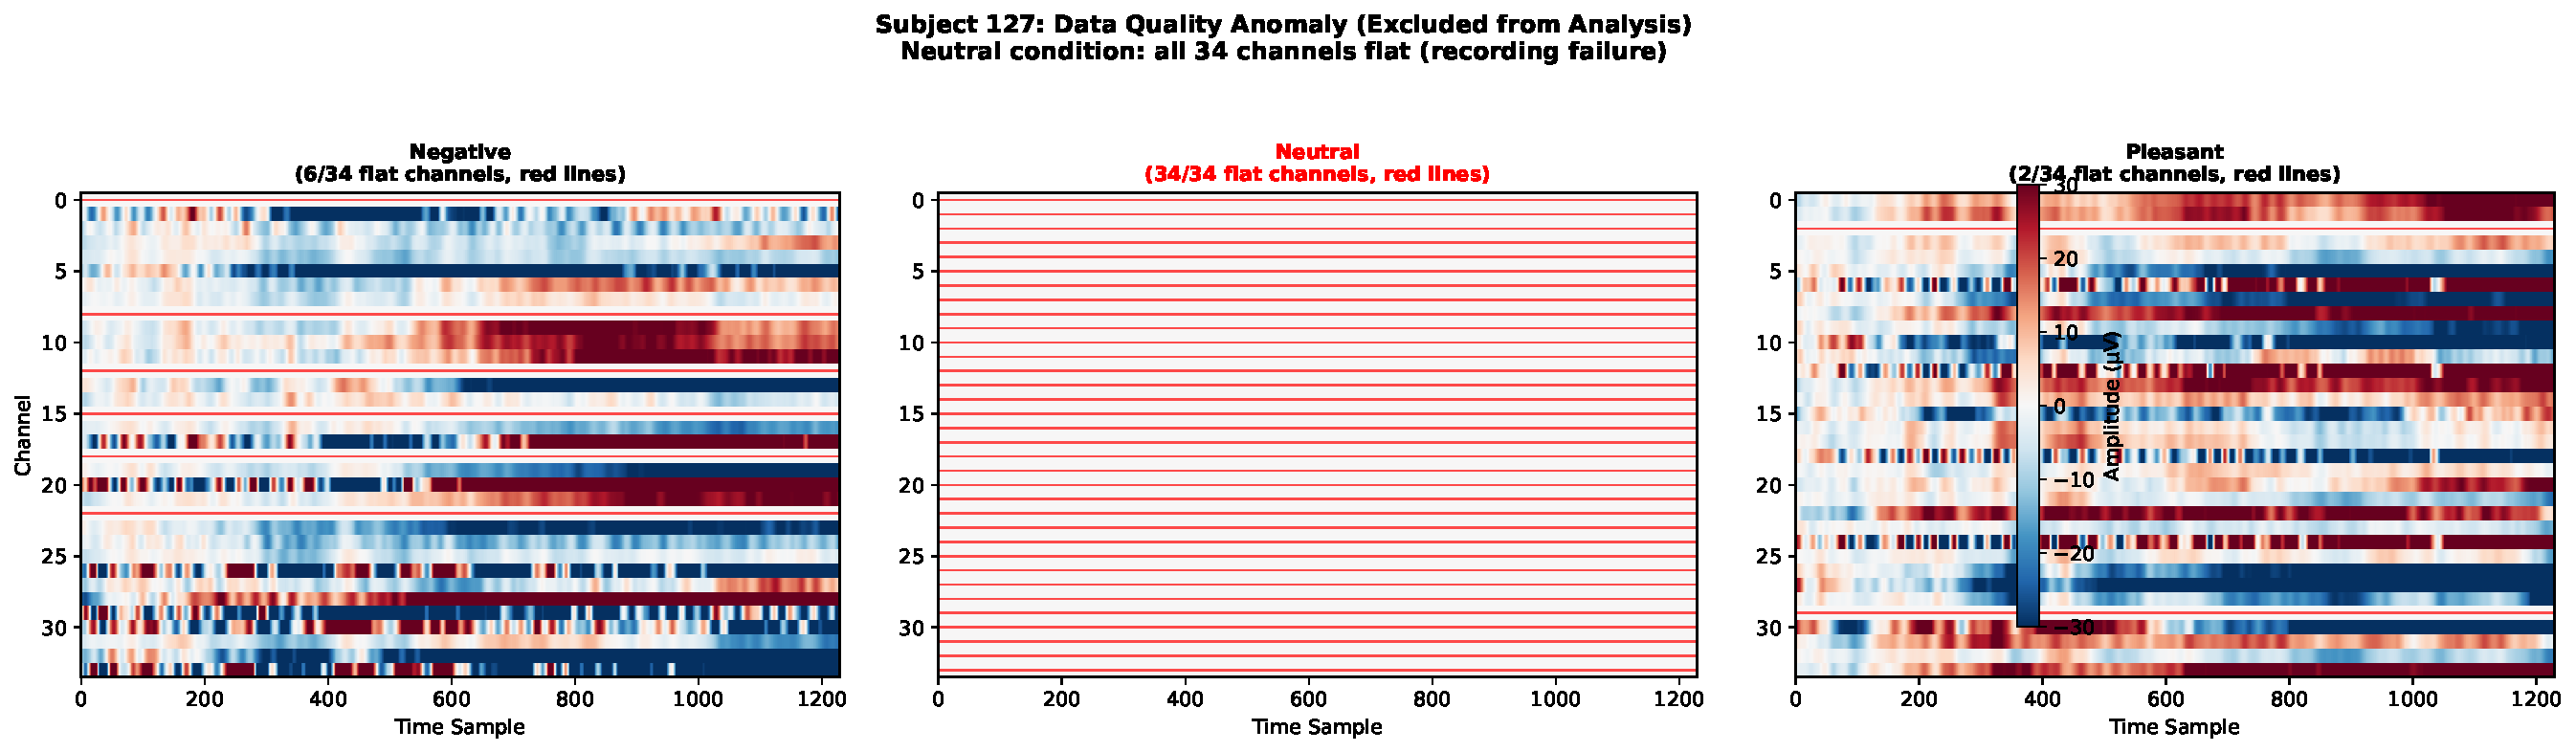
\includegraphics[width=\textwidth]{pictures/chGraphNeuralNetworks/fig_qc_subject127_anomaly.pdf}
    \caption{Subject~$127$ recording anomaly. The Neutral condition is entirely flat across all $34$ channels. Red lines indicate flat channels. This subject was excluded from all analyses.}
    \label{fig:qc_subject127}
\end{figure}

The final dataset comprises $\mathbf{211}$ \textbf{subjects} $\times$ $\mathbf{3}$ \textbf{conditions} $= \mathbf{633}$ \textbf{observations}.

\subsection{Clinical Metadata}

The clinical metadata include $142$ participants with Major Depressive Disorder ($67.3\%$), $82$ with PTSD ($38.9\%$), $85$ with Substance Use Disorder ($40.3\%$), $60$ with GAD ($28.4\%$), $50$ with ADHD ($23.7\%$), $69$ with eating disorders ($32.7\%$), $34$ with mania ($16.1\%$), and $91$ taking psychiatric medication ($43.1\%$). Sex was recorded as female for $172$ participants and male for $33$; six records were unavailable or not represented in those two counts. Mean comorbidity burden is $2.8$ diagnoses per subject (range $0$--$7$).

\begin{figure}[H]
    \centering
    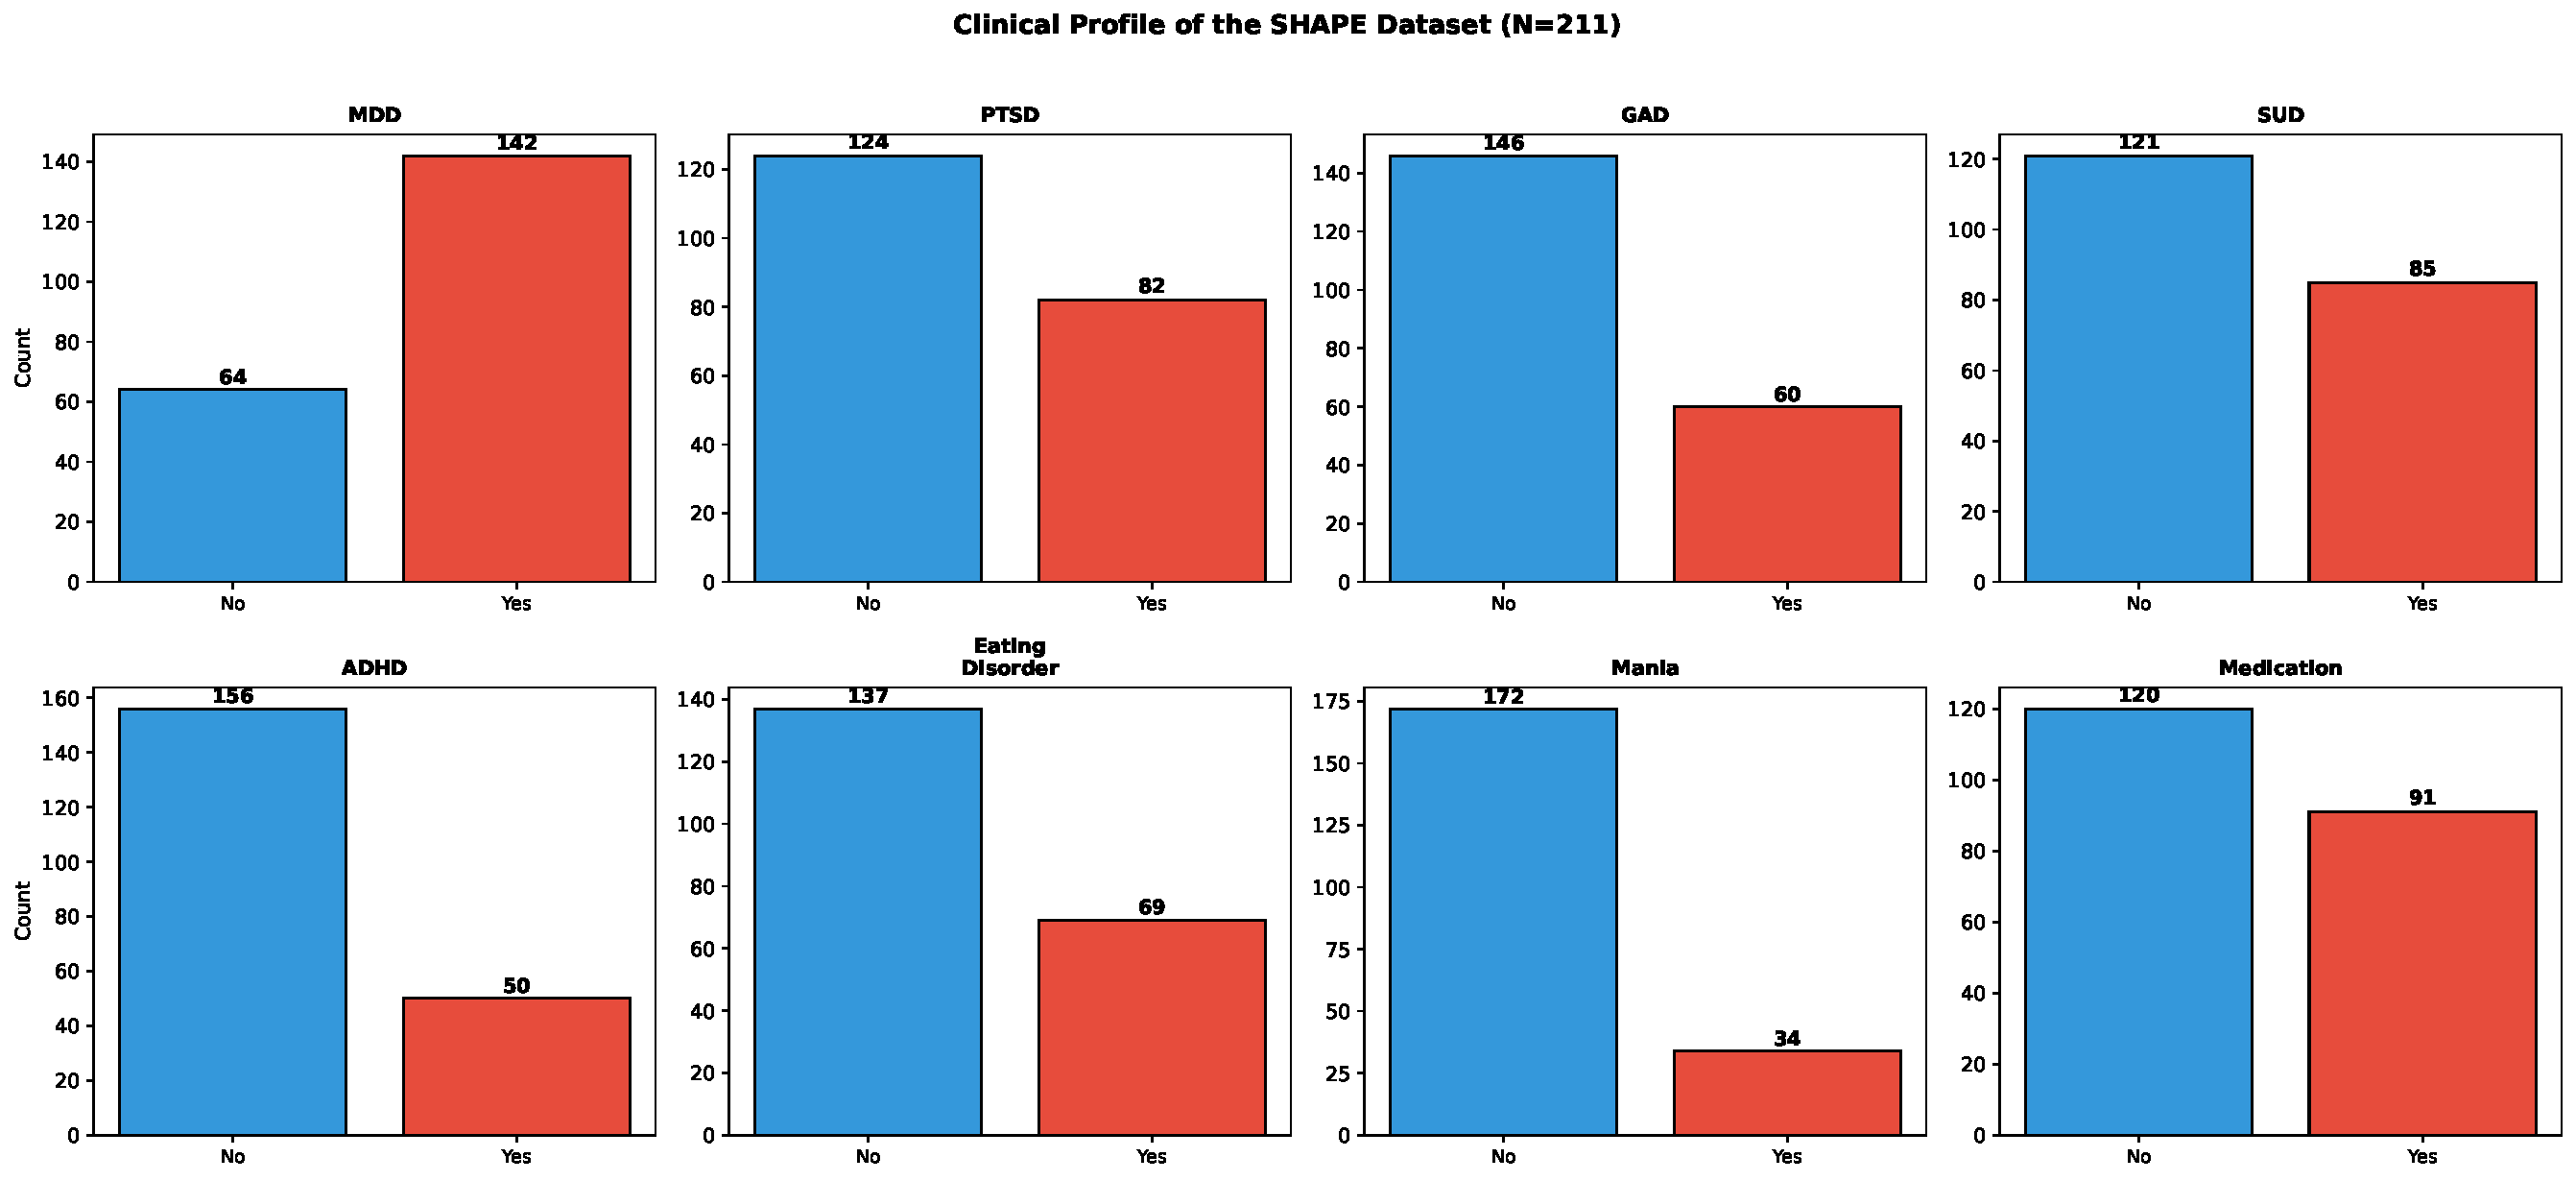
\includegraphics[width=\textwidth]{pictures/chGraphNeuralNetworks/fig_clinical_profile_211.pdf}
    \caption{Clinical profile of the $211$ SHAPE subjects. Eight diagnostic variables with group sizes.}
    \label{fig:clinical_profile}
\end{figure}

\subsection{Preprocessing Pipeline}

Four steps transform each $1229 \times 34$ trial-averaged ERP matrix into the reservoir format: removal of the first $205$ rows, $4\times$ anti-aliasing decimation to $256$~Hz ($256$ post-baseline samples), per-channel z-score normalization, and reservoir processing ($N_{\text{res}}=256$, $\beta=0.05$, $M_{\text{th}}=0.5$). The archived primary extractor divided all 256 samples into six 42-sample bins and omitted the four-sample remainder. That full-epoch BSC$_6$ differs from the steps 10--70 early-window specification in Chapter~\ref{chap:embeddings} and from the later attention analysis. The corrected code uses the stated early window and fits a common PCA-64 basis only on each training fold. The raw inputs were unavailable for rerunning it, so the numerical results below retain the archived full-epoch encoding and global PCA unless explicitly identified as the separate early-window analysis.


\section{Raw Data Observations}
\label{sec:ch5_raw_obs}

Before classification and clinical analysis, this section records summaries at each pipeline stage: z-scored trial-averaged EEG, reservoir spikes, the archived PCA-64 geometry, channel-feature similarity, and variation in the thresholded graphs. The figures are descriptive and inherit the preprocessing limitations stated above.

\subsection{Multichannel EEG Entering the Graph Stage}

The preprocessed dataset provides $633$ condition-level observations ($211$ participants $\times$ $3$ conditions), each a $256 \times 34$ matrix of z-scored amplitudes at $256$~Hz. Figure~\ref{fig:obs01_eeg} displays three selected participants. After per-channel z-scoring, the pooled distribution is centered at $0.000$ with unit variance and a range of $[-5.41, 5.01]$. Waveform morphology differs across the displayed participants. Because each participant contributes three rows, all predictive splits must keep a participant's rows together.

\begin{figure}[H]
    \centering
    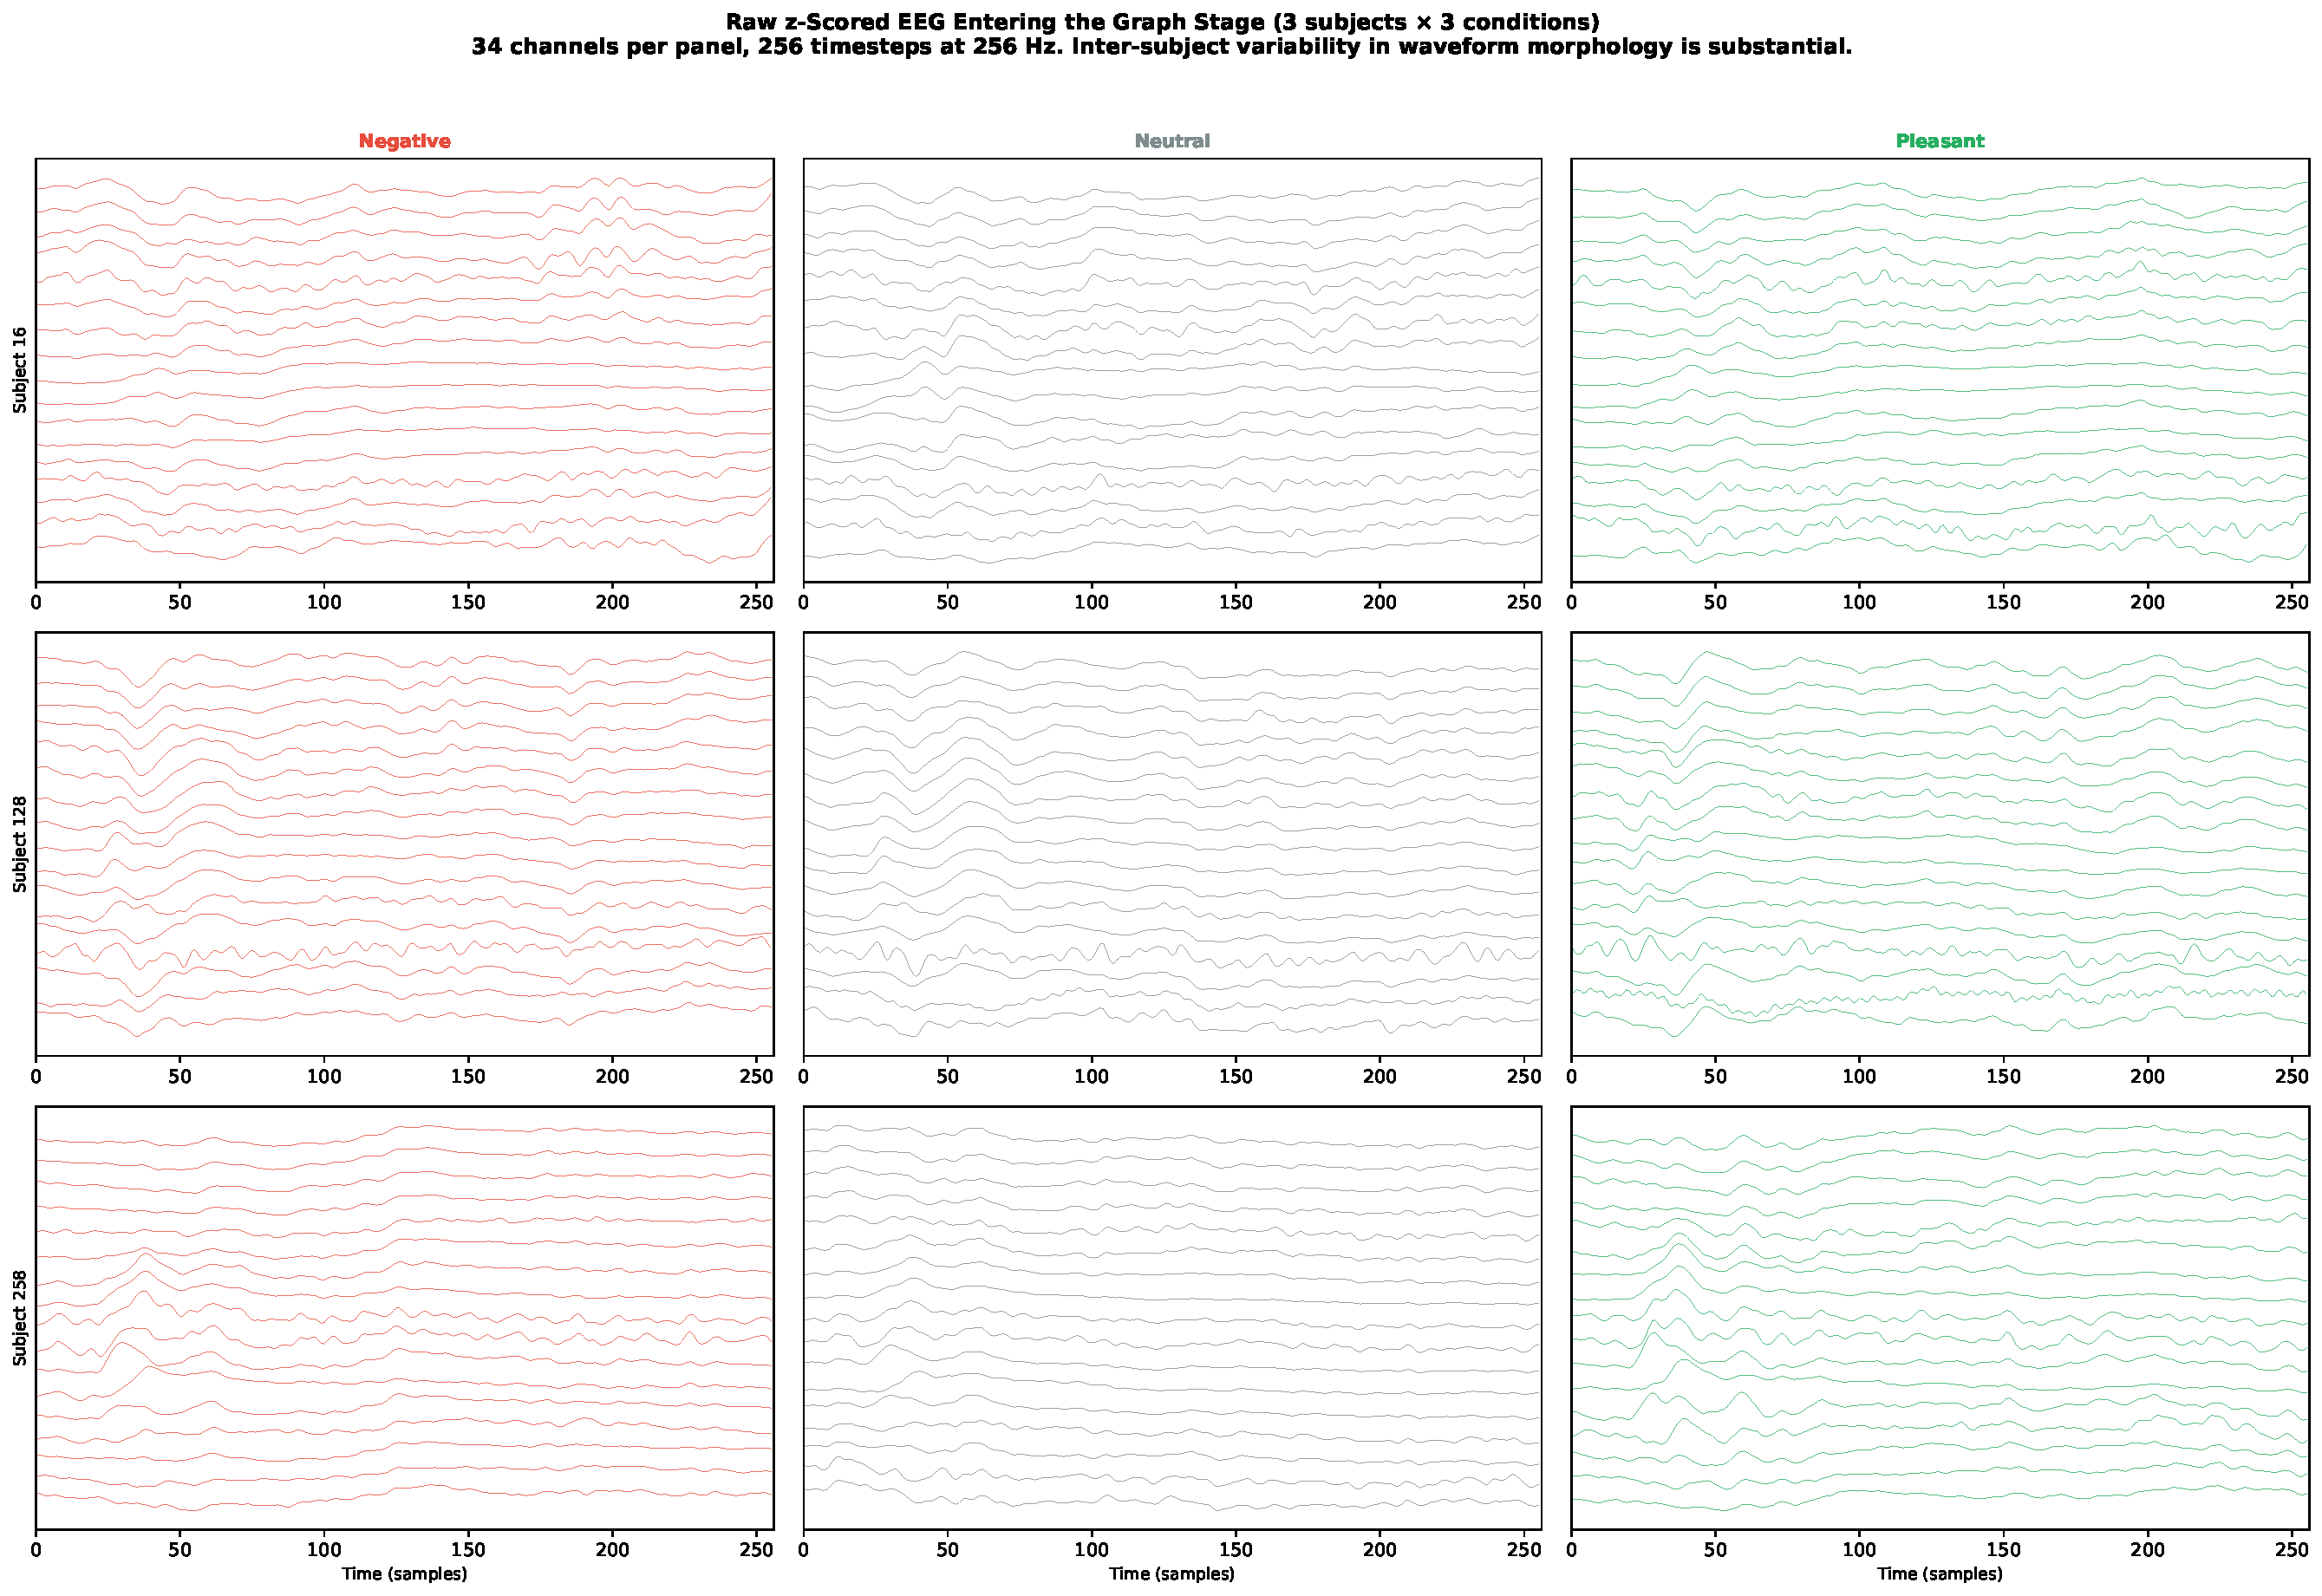
\includegraphics[width=\textwidth]{pictures/chGraphNeuralNetworks/obs01_raw_eeg_waveforms.pdf}
    \caption{Selected z-scored, trial-averaged EEG inputs ($3$ participants $\times$ $3$ conditions). Each panel shows $17$ of $34$ channels offset vertically over $256$ time steps. The examples illustrate both between-participant and within-participant differences but do not estimate their population ratio.}
    \label{fig:obs01_eeg}
\end{figure}

\subsection{Reservoir Spike Response on Real EEG}

Figure~\ref{fig:obs02_spikes} shows the reservoir response for one selected participant under all three conditions. The top row contains spike rasters for Channel~10, and the bottom row contains population firing-rate traces for four channels. Across the full SHAPE feature array, $47.4\%$ of BSC$_6$ entries are zero, compared with $79.1\%$ for the synthetic generator. The mean entry is $5.15$, and the maximum is $42$ spikes per neuron per bin. These values describe the different input distributions; they do not isolate why their sparsity differs.

\begin{figure}[H]
    \centering
    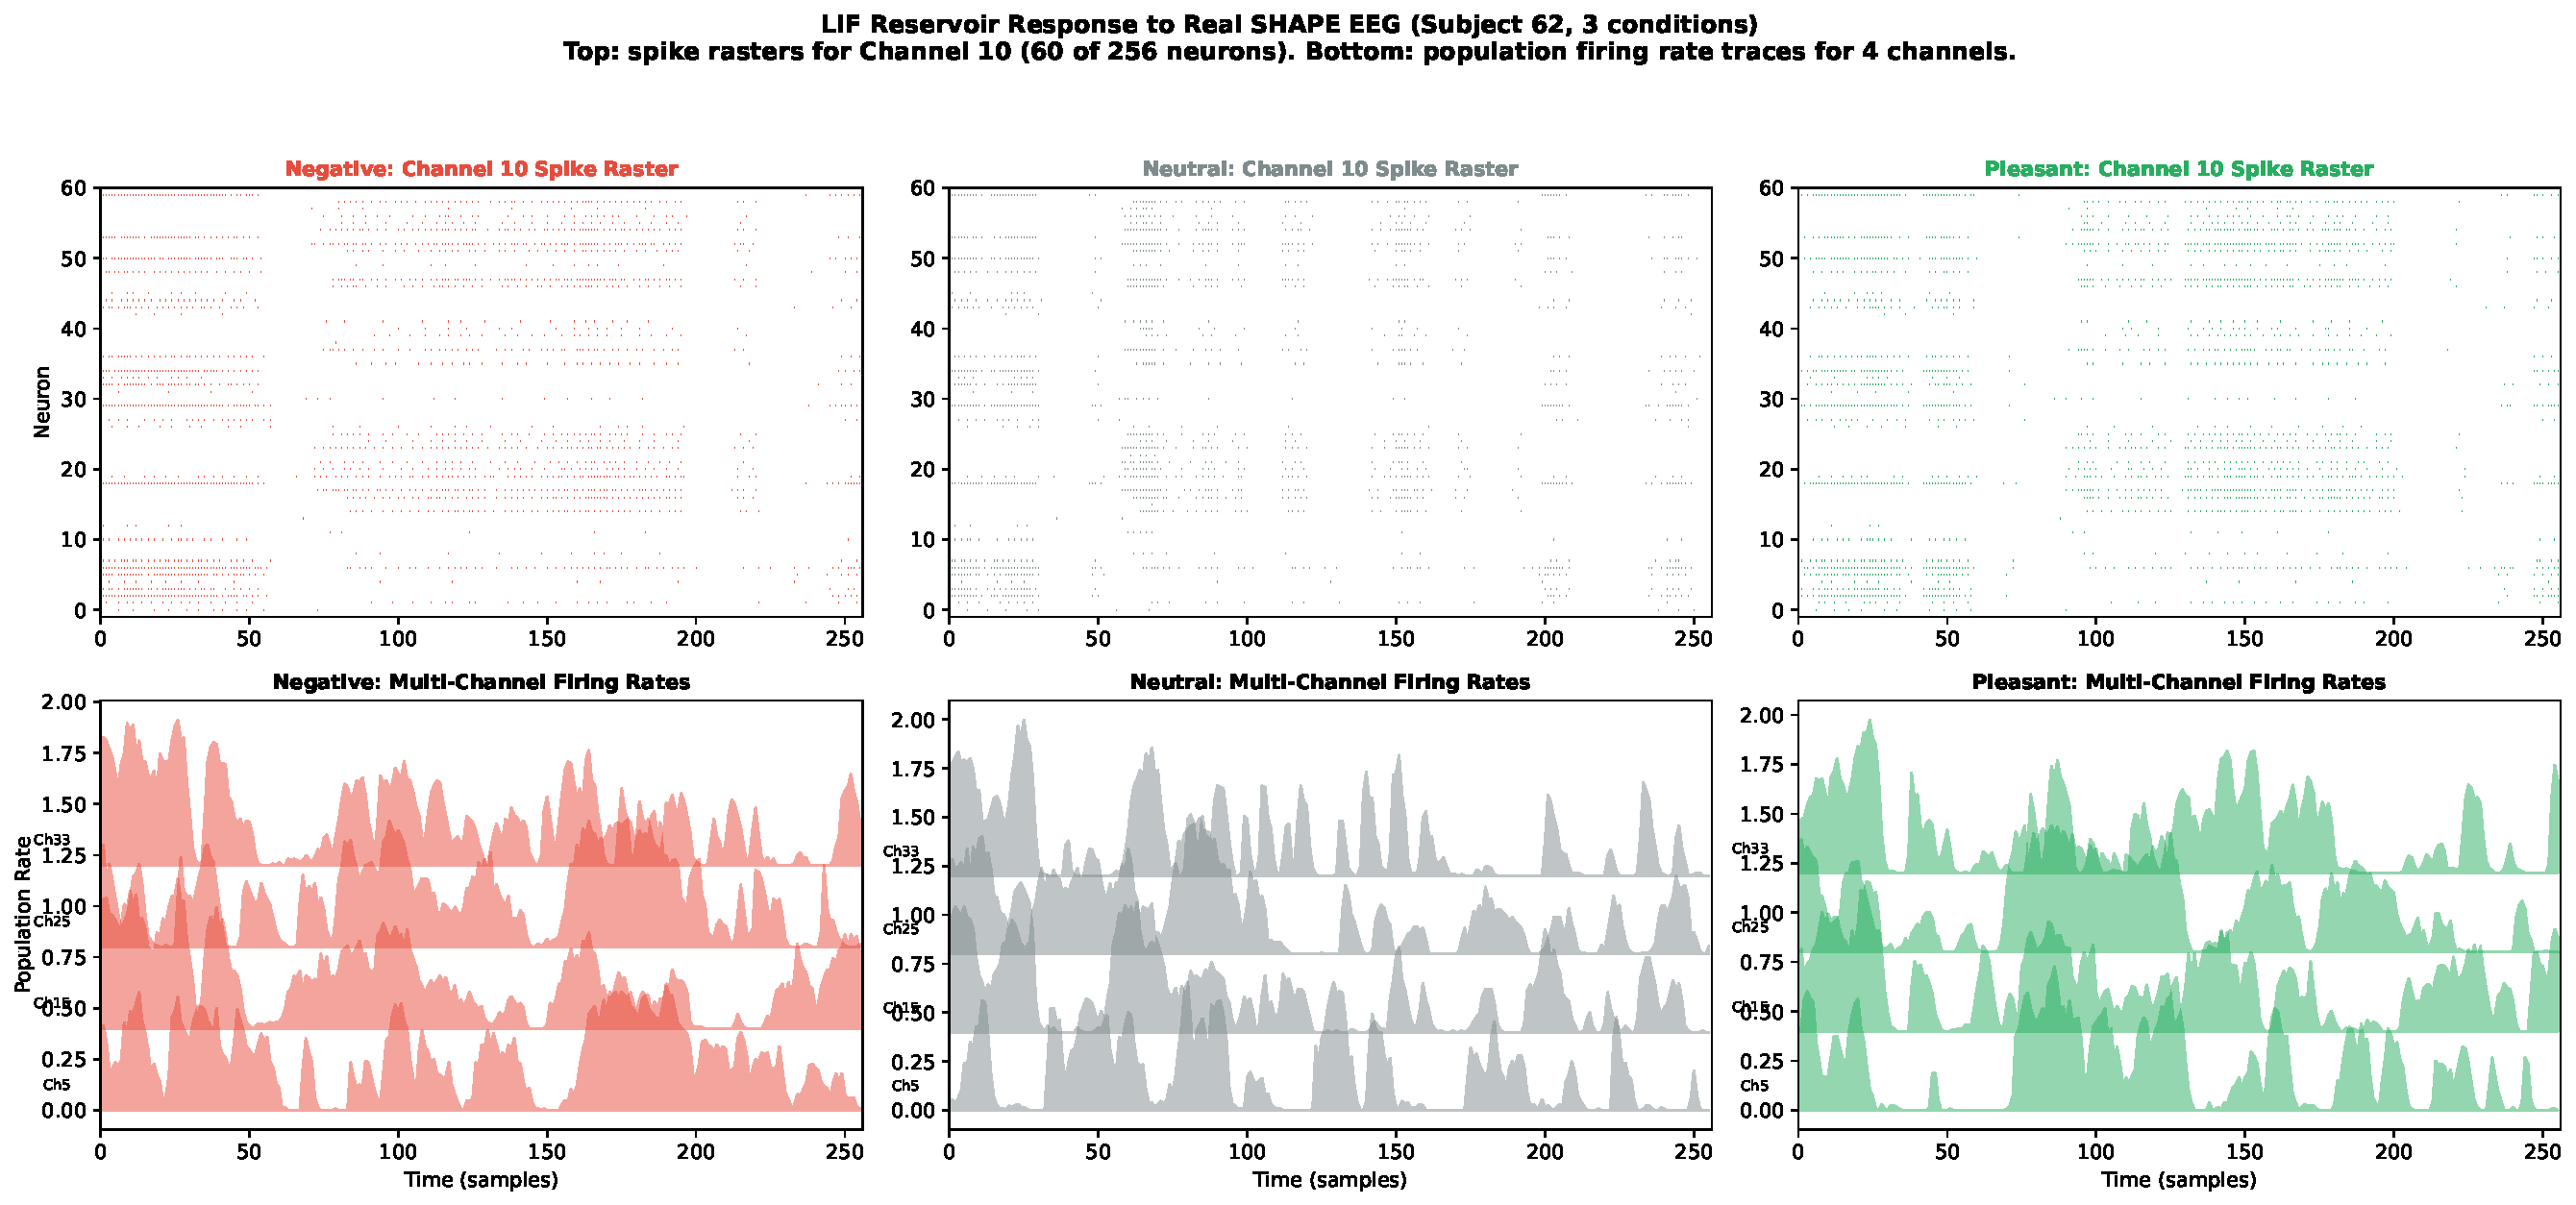
\includegraphics[width=\textwidth]{pictures/chGraphNeuralNetworks/obs02_raw_spike_trains.pdf}
    \caption{Reservoir response to SHAPE EEG for one participant and three conditions. Top: spike rasters for Channel~10 ($60$ of $256$ units). Bottom: population firing-rate traces for four channel indices.}
    \label{fig:obs02_spikes}
\end{figure}

\subsection{PCA-64 Embedding Geometry}

Figure~\ref{fig:obs03_embeddings} characterizes the archived PCA-64 embedding space. The left panel projects the concatenated $34 \times 64 = 2{,}176$-dimensional embeddings into two dimensions, colored by emotional condition; the conditions overlap substantially. The center panel colors the same projection by subject identity and shows tighter within-subject grouping. The right panel shows per-channel embedding variance, ranging from $36{,}900$ (Channel~16) to $70{,}721$ (Channel~29), with a coefficient of variation of $0.15$. These are in-sample geometric summaries of the global-PCA representation and should not be read as held-out evidence.

\begin{figure}[H]
    \centering
    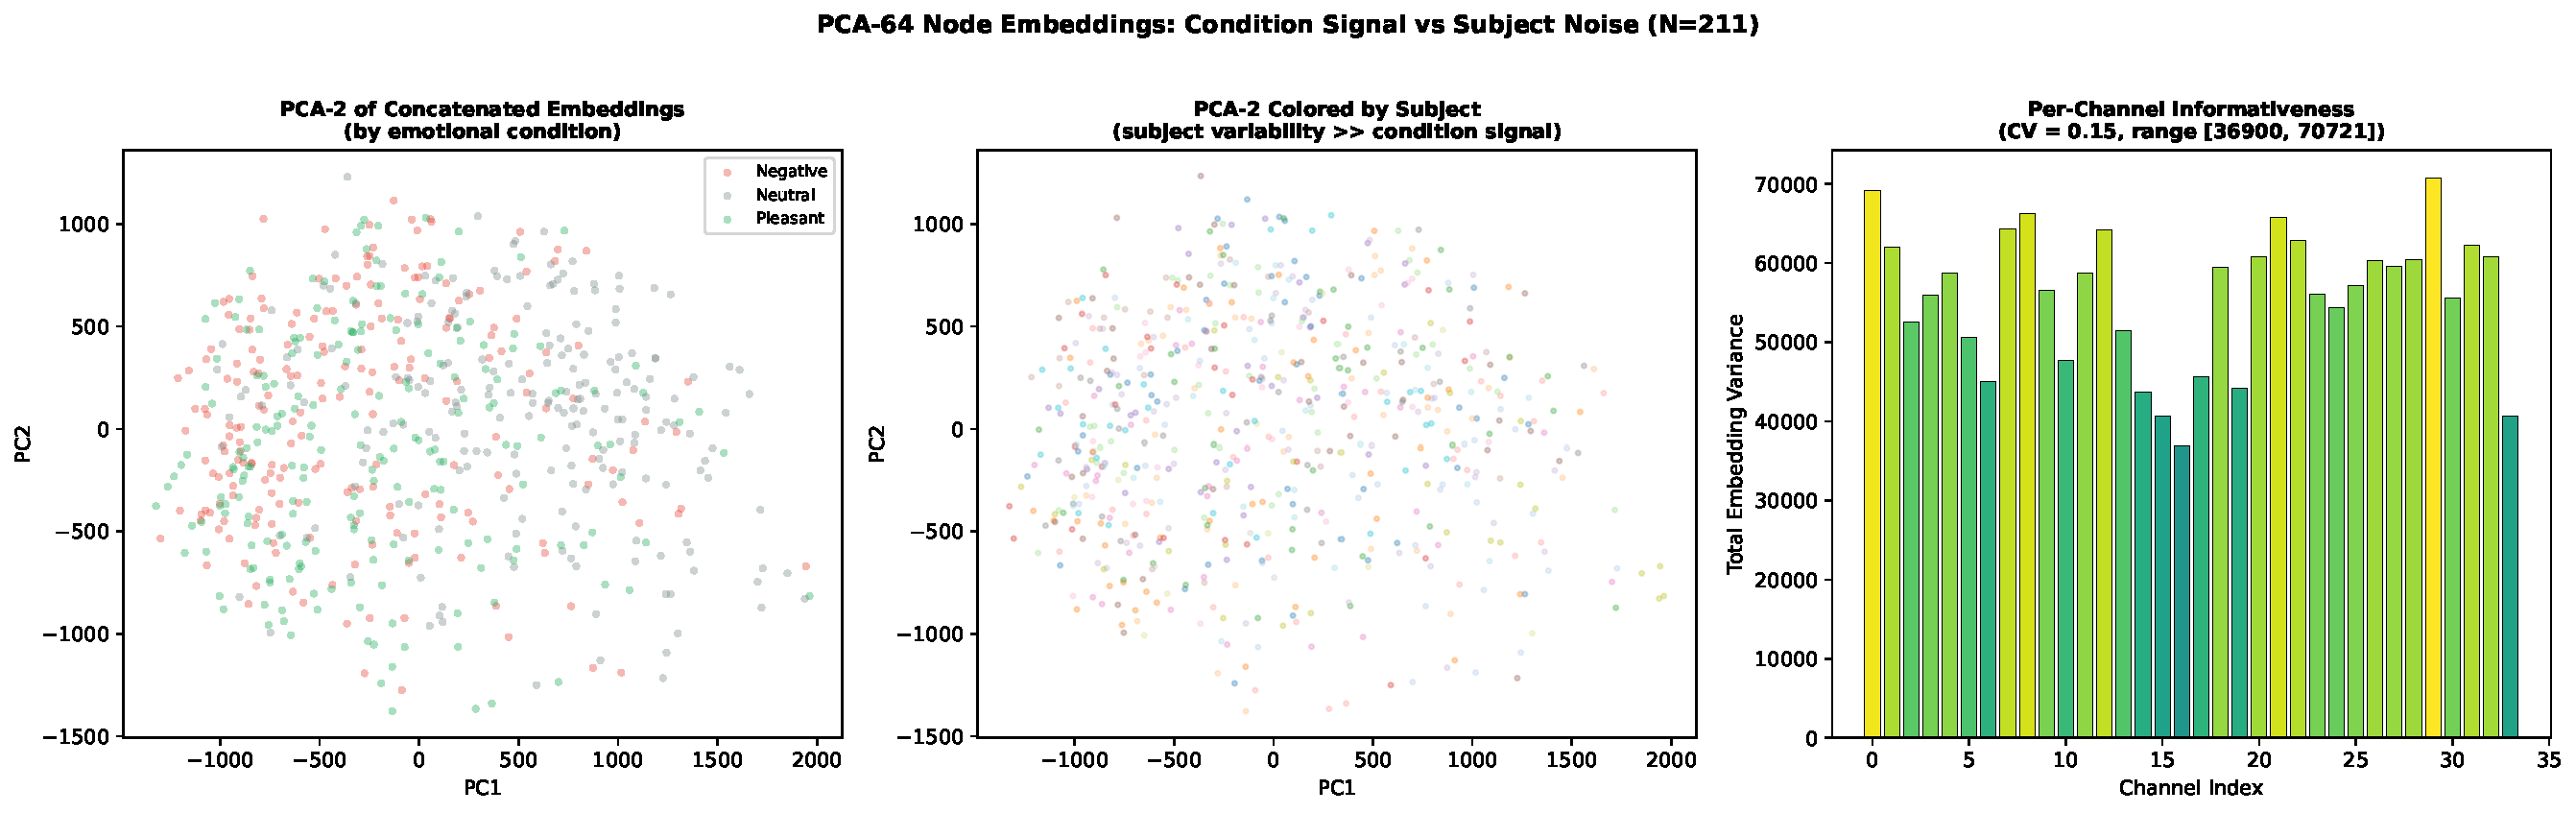
\includegraphics[width=\textwidth]{pictures/chGraphNeuralNetworks/obs03_bsc6_pca64_embeddings.pdf}
    \caption{Archived PCA-64 embedding geometry ($N = 211$). Left: PCA-2 by condition. Center: PCA-2 by subject. Right: per-channel embedding variance. PCA was fitted globally for this descriptive figure.}
    \label{fig:obs03_embeddings}
\end{figure}

\subsection{Archived Inter-Channel Feature Similarity}

Figure~\ref{fig:obs04_connectivity} displays the archived correlations between per-channel PCA coordinate vectors and the resulting thresholded graphs. The mean displayed correlation is $\bar{r}=0.143$ (SD $0.552$). Because each channel's PCA basis was fitted separately, coordinate positions do not have a shared meaning across channels. These values describe the archived numerical construction only and are not estimates of EEG channel connectivity.

At the fixed $20\%$ density threshold, each condition-average graph contains $113$ edges, with mean degree $6.6$. Terms such as ``hub,'' ``clustering,'' and ``component'' below refer to this mathematical similarity graph, not to anatomical hubs or communication in a brain network.

\begin{figure}[H]
    \centering
    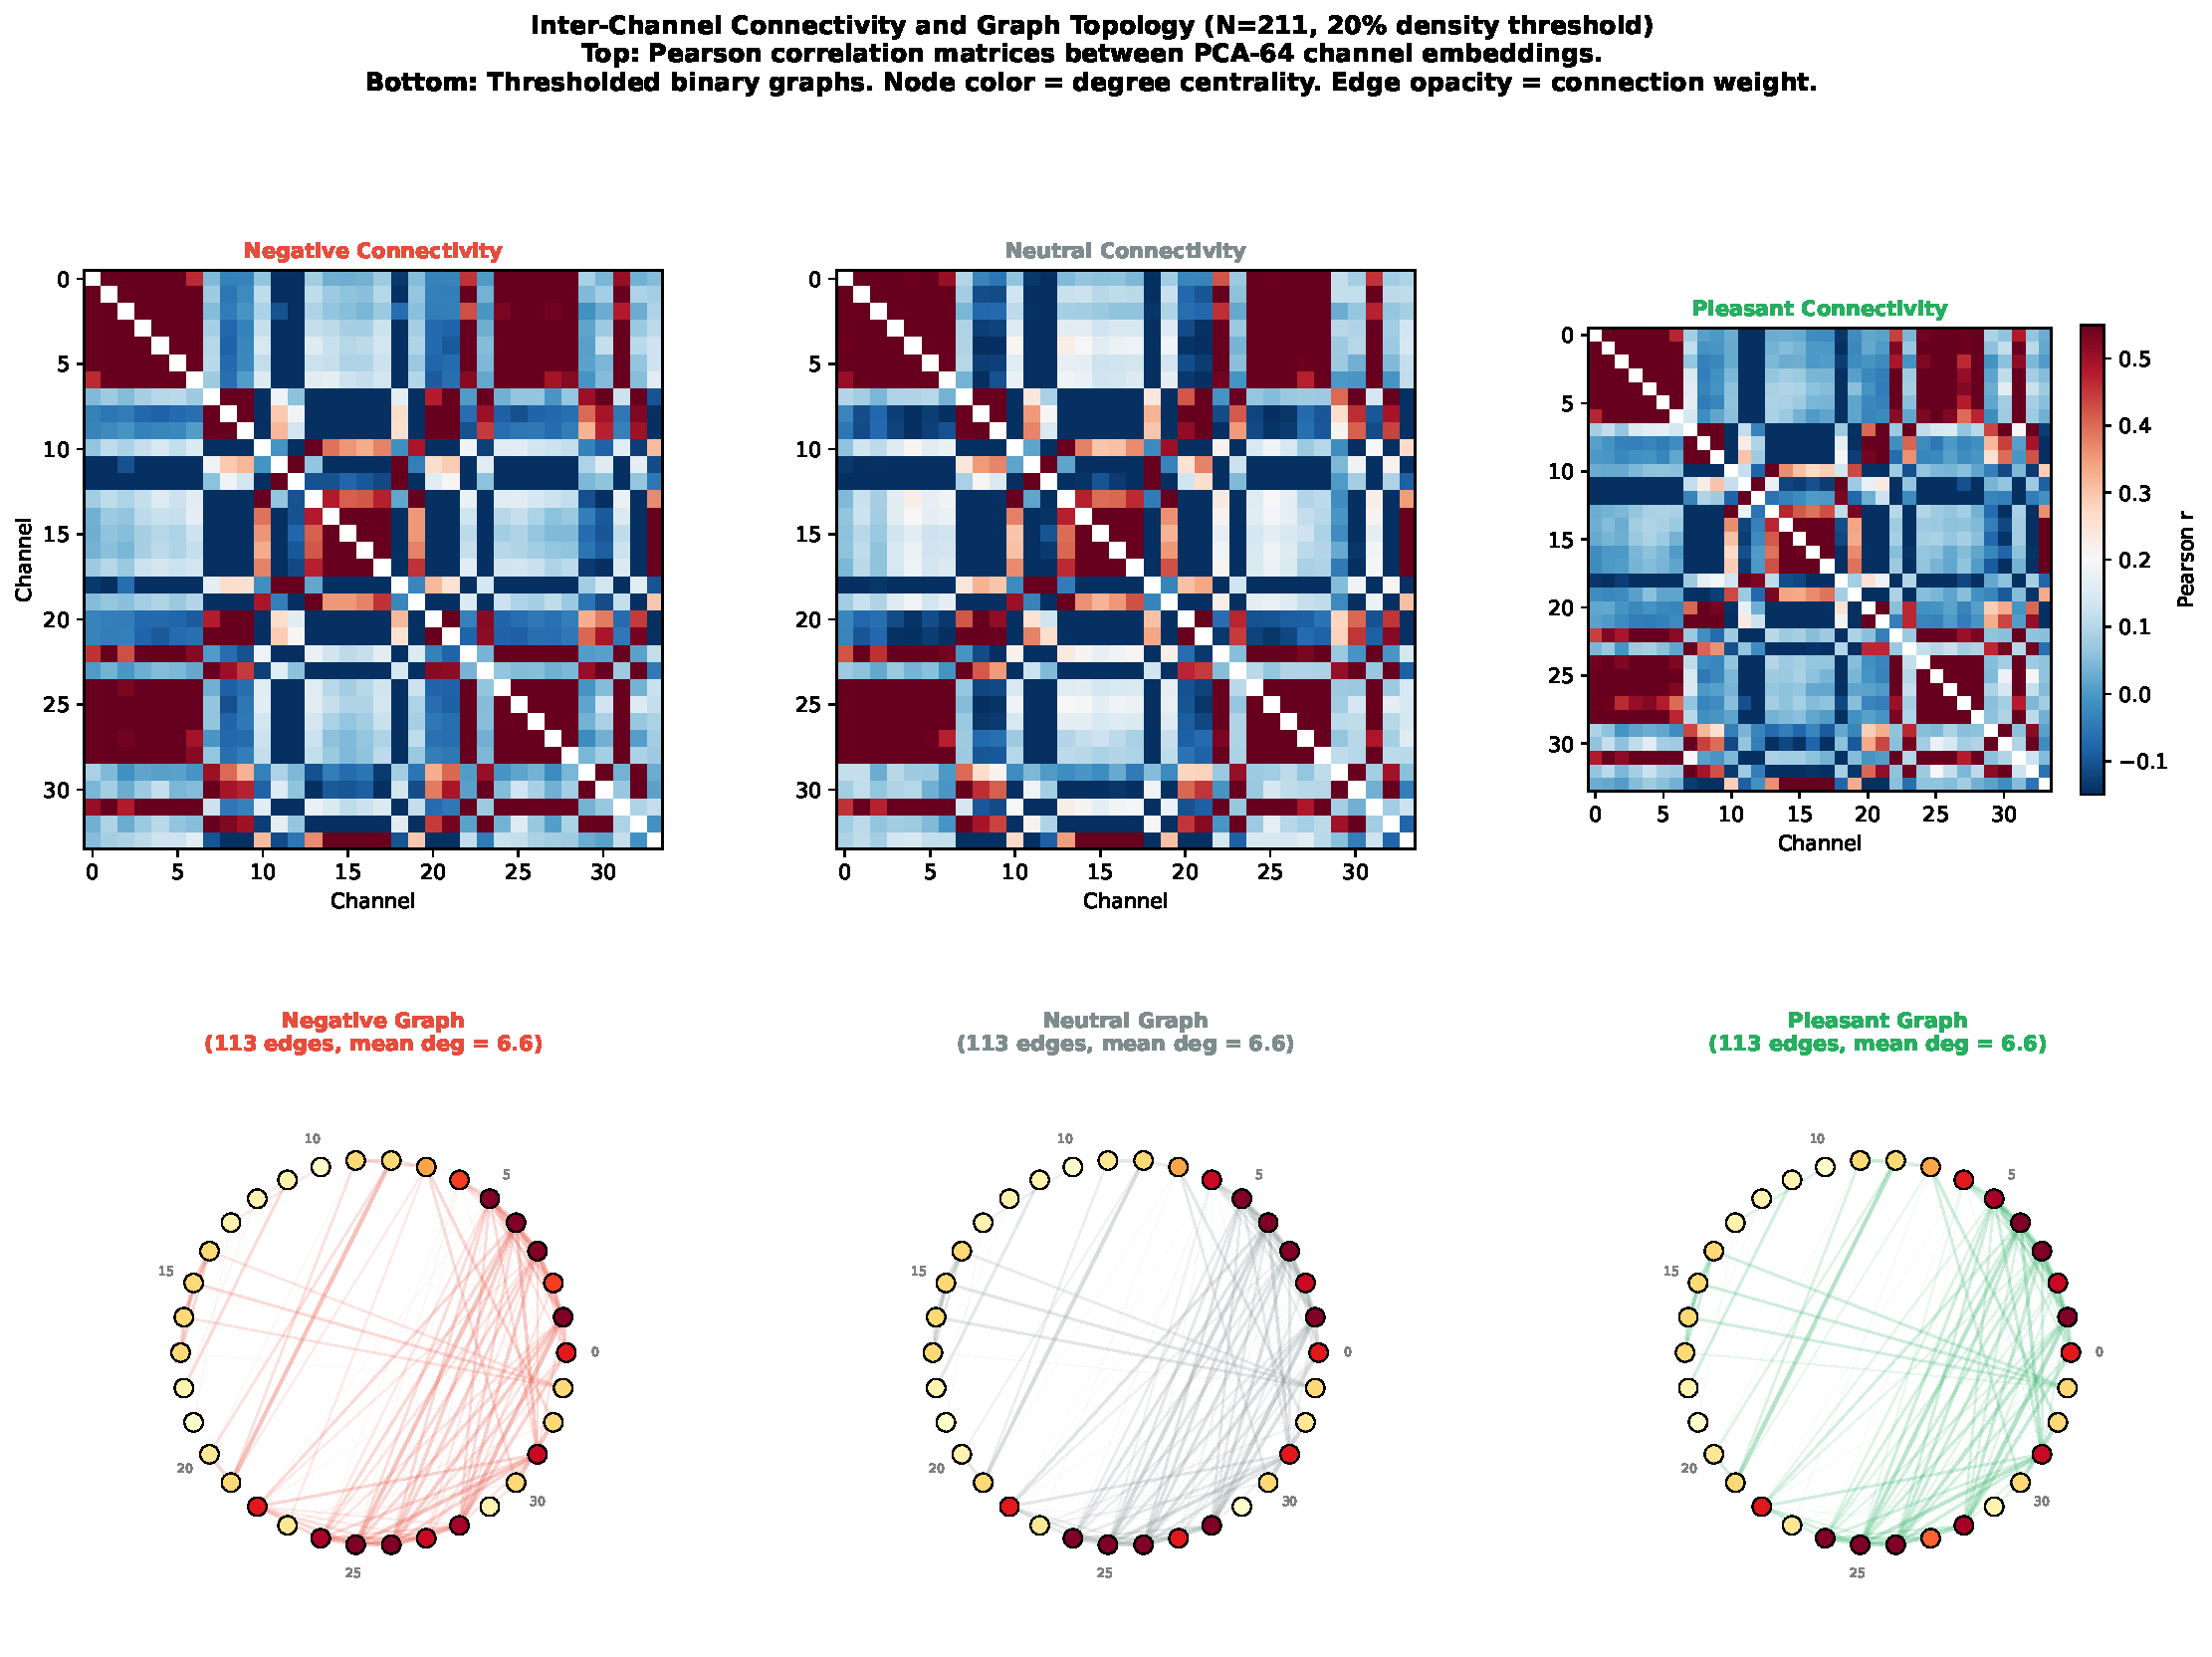
\includegraphics[width=\textwidth]{pictures/chGraphNeuralNetworks/obs04_raw_connectivity_matrices.pdf}
    \caption{Archived cross-channel PCA-coordinate similarity and thresholded graphs ($N=211$, $20\%$ density). Separately fitted channel PCA axes are not commensurate; the figure is retained as a record of the legacy construction and has no physiological-connectivity interpretation.}
    \label{fig:obs04_connectivity}
\end{figure}

\subsection{Between-Subject Graph Variability}

Figure~\ref{fig:obs07_variability} records between-participant variation in the archived graph construction. The selected graphs have different edge and degree patterns under the same $20\%$ density rule. The displayed edge-weight standard deviation is $0.303$, and degrees across participant--channel combinations range from $0$ to $15$ with mean $6.6$.

The Negative-minus-Pleasant panel shows differences in the archived similarity values. Between-subject variability ($\sigma=0.303$) is approximately seven times the mean absolute condition difference ($|\Delta r|=0.045$). This descriptive ratio is not a signal-to-noise estimate and does not establish either a physiological condition signal or inter-individual brain-network organization.

\begin{figure}[H]
    \centering
    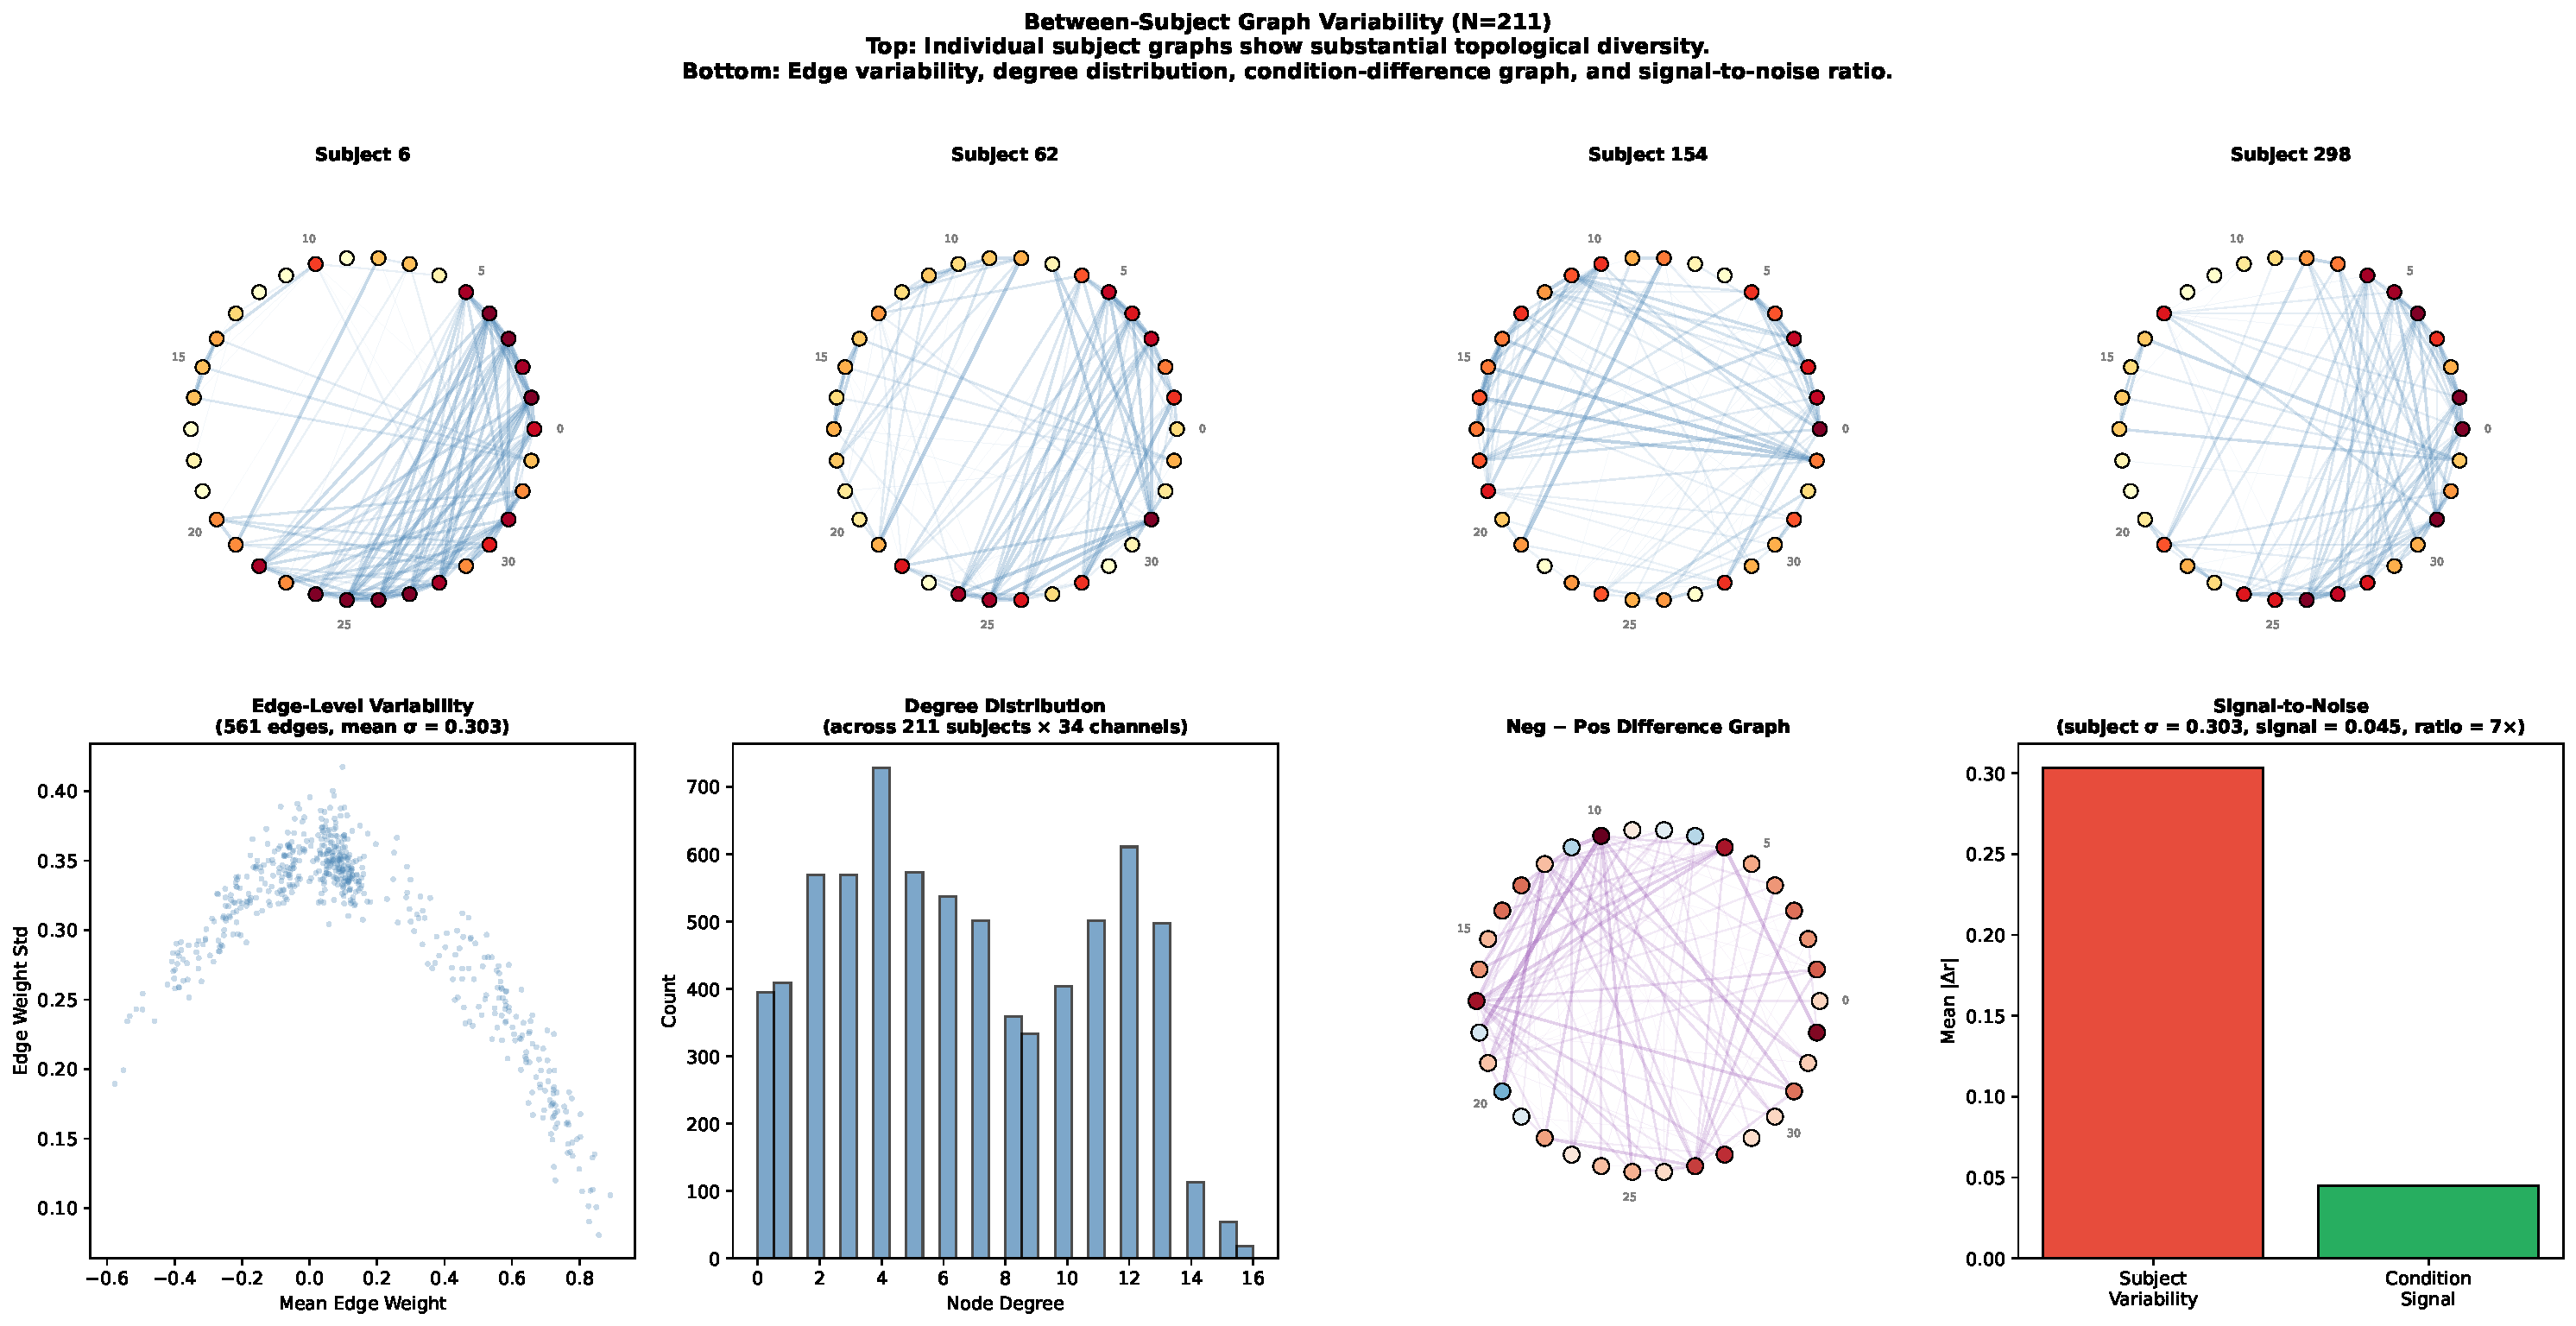
\includegraphics[width=\textwidth]{pictures/chGraphNeuralNetworks/obs07_graph_variability.pdf}
    \caption{Variability of the archived thresholded similarity graphs ($N=211$). The displayed sevenfold ratio compares two summary scales; it is not a formal signal-to-noise ratio.}
    \label{fig:obs07_variability}
\end{figure}

The descriptive figures show substantial between-subject variation, overlapping condition projections, and broad archived similarity values. Because of the global and noncommensurate PCA construction, these plots should be used to understand the legacy analysis rather than to infer heterophily or physiological network structure.

\subsection{The Reservoir's Spike Representation on Real EEG}

Figure~\ref{fig:obs13_bsc6} characterizes the BSC$_6$ features produced from the trial-averaged SHAPE inputs. Each observation is a $34 \times 256 \times 6$ tensor ($34$ channels, $256$ reservoir units, $6$ temporal bins), yielding $52{,}224$ spike-count features. The array is $47.4\%$ zero, compared with $79.1\%$ for the synthetic task in Chapter~\ref{chap:embeddings}. Nonzero entries have mean $9.79$, median $7$, and maximum $42$ spikes per unit per bin.

\begin{figure}[H]
    \centering
    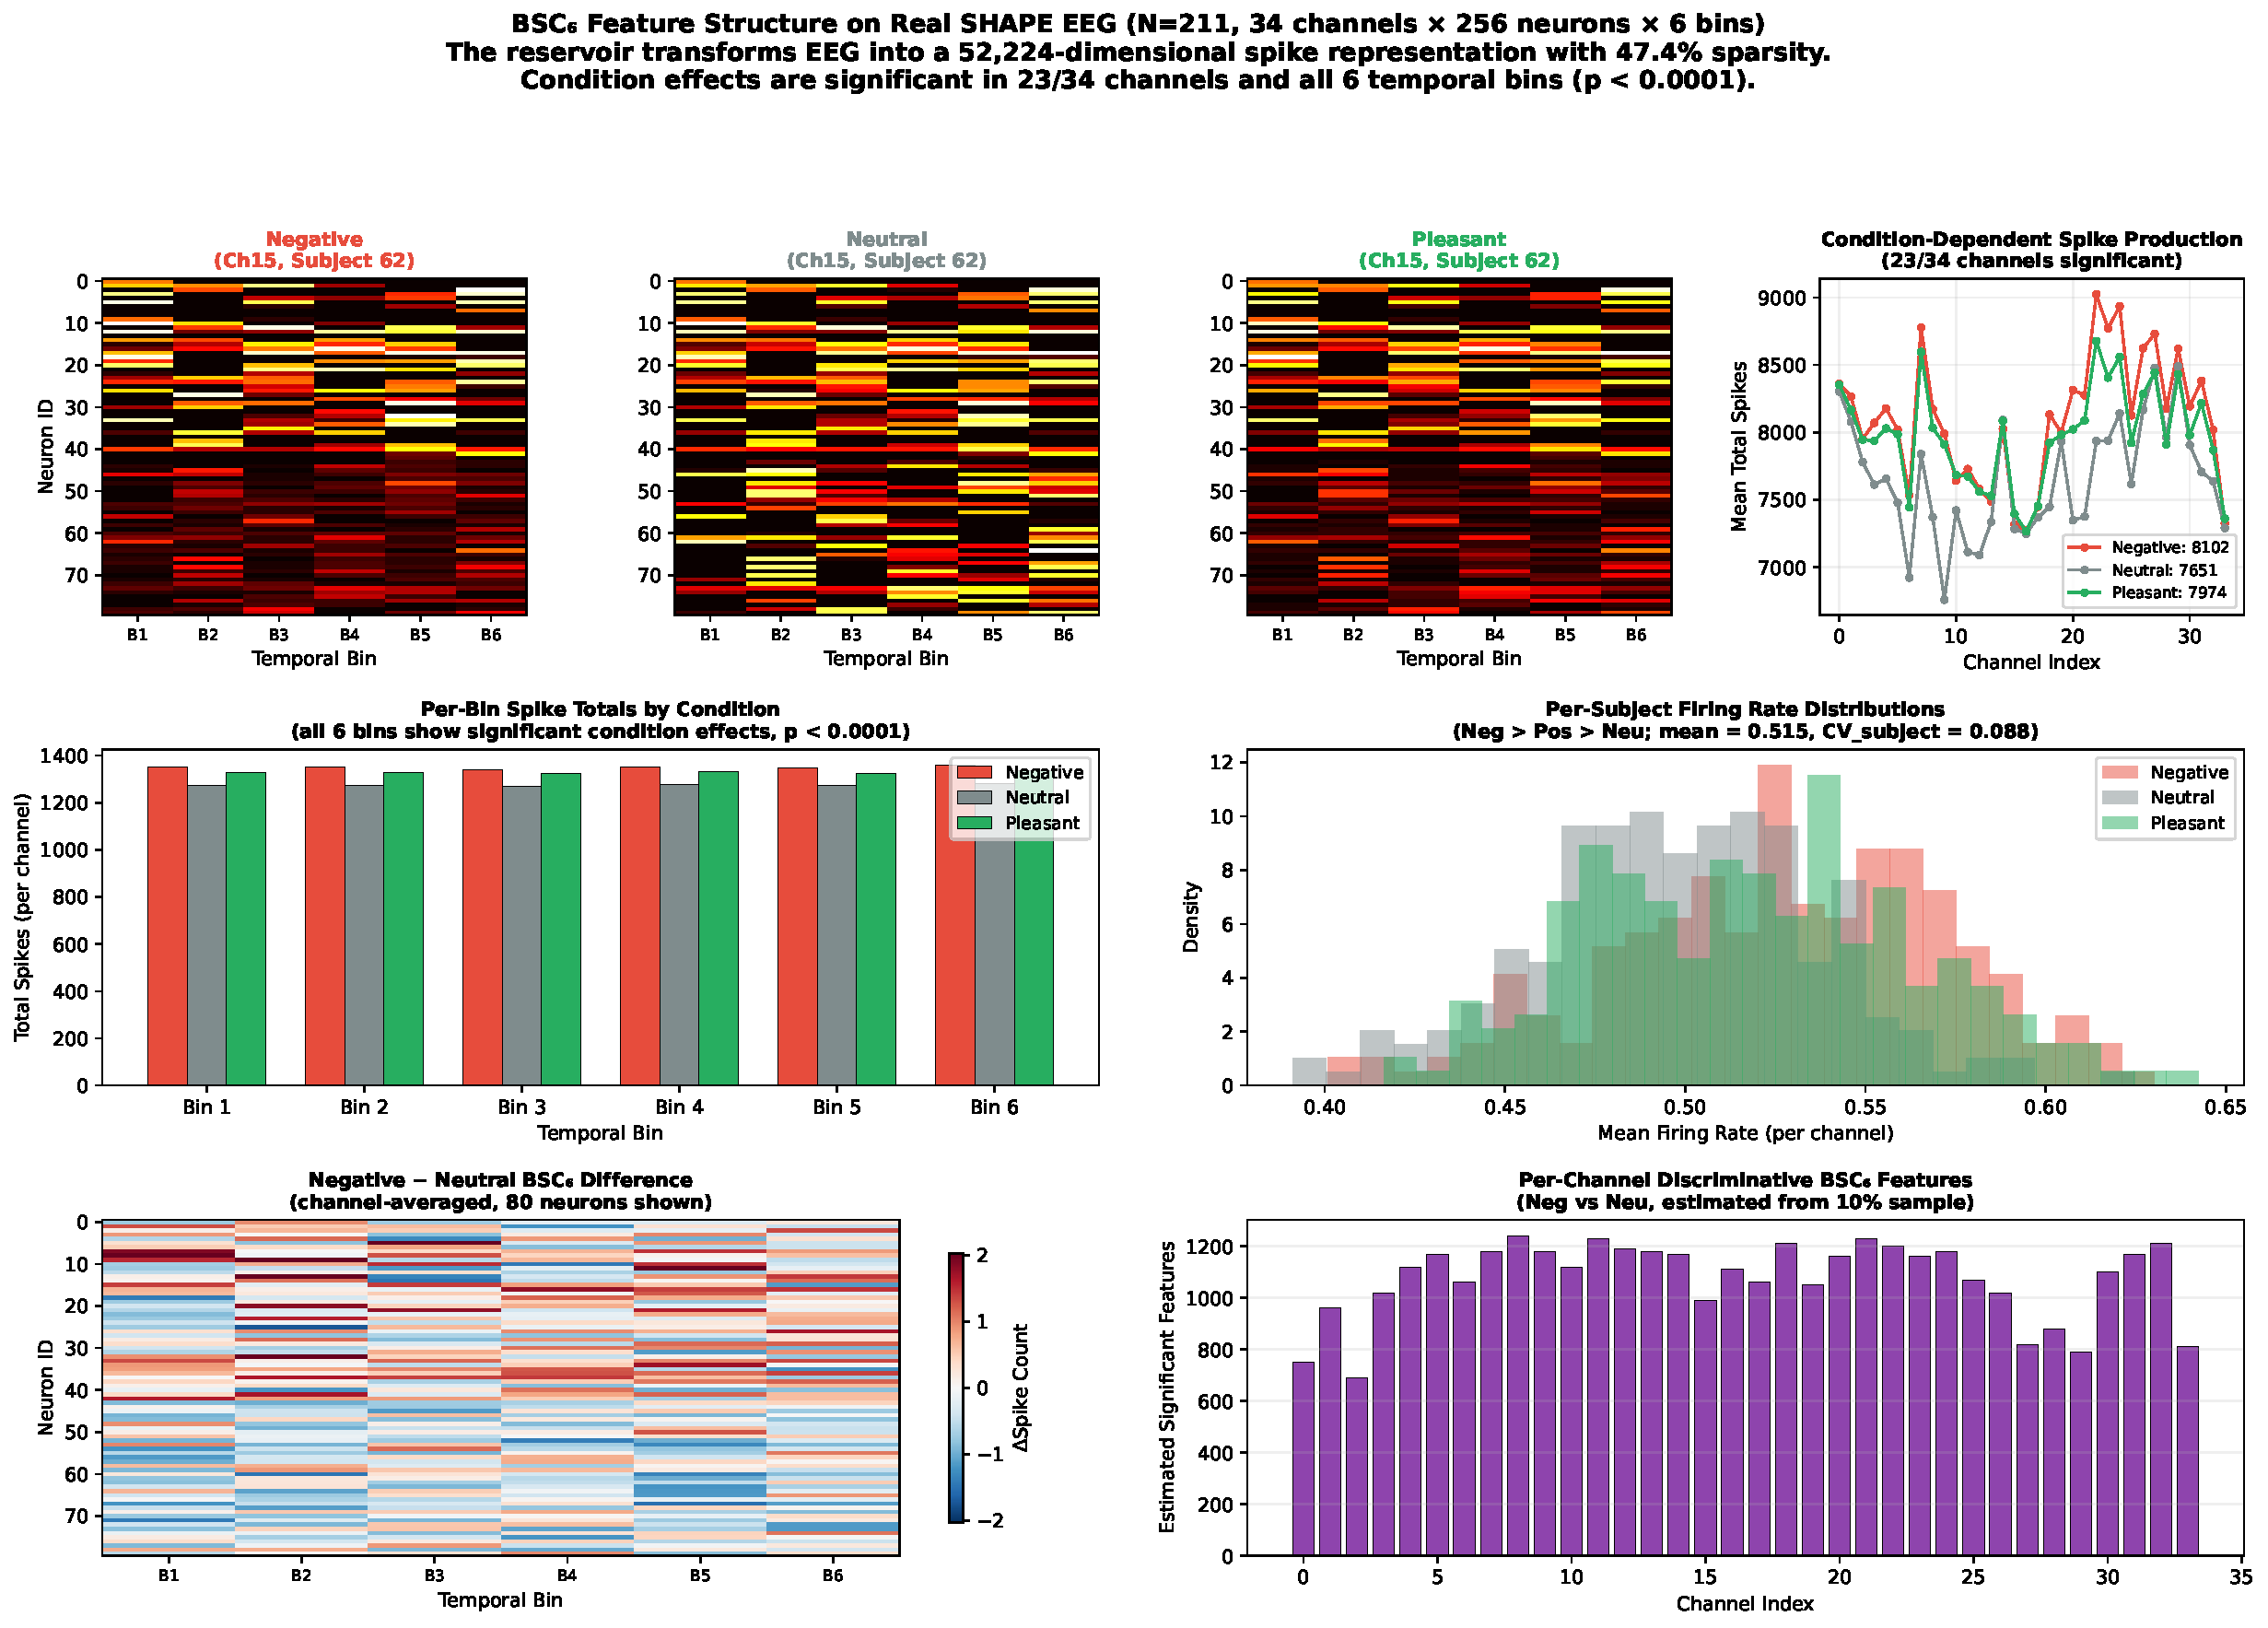
\includegraphics[width=\textwidth]{pictures/chGraphNeuralNetworks/obs13_bsc6_real_eeg.pdf}
    \caption{BSC$_6$ features on SHAPE EEG ($N=211$). The channel and bin $p$ values shown in the archived figure are nominal and were not adjusted as one prespecified family.}
    \label{fig:obs13_bsc6}
\end{figure}

The archived full-epoch summaries are Negative $8{,}102\pm1{,}220$, Neutral $7{,}651\pm1{,}153$, and Pleasant $7{,}974\pm1{,}175$ spikes per channel. Nominal channel and bin tests produce small $p$ values, but the family was not prespecified or multiplicity adjusted. These bins each span 42 samples (about 164~ms) across samples 0--251; four trailing samples are omitted. They must not be interpreted using the 39--273~ms early-window labels reported in the later traceability analysis.

\subsection{Geometry Before and After Panel Centering}

Figure~\ref{fig:obs14_geometry} compares pairwise distances in the archived representation before and after subtracting each participant's three-observation mean.

\begin{figure}[H]
    \centering
    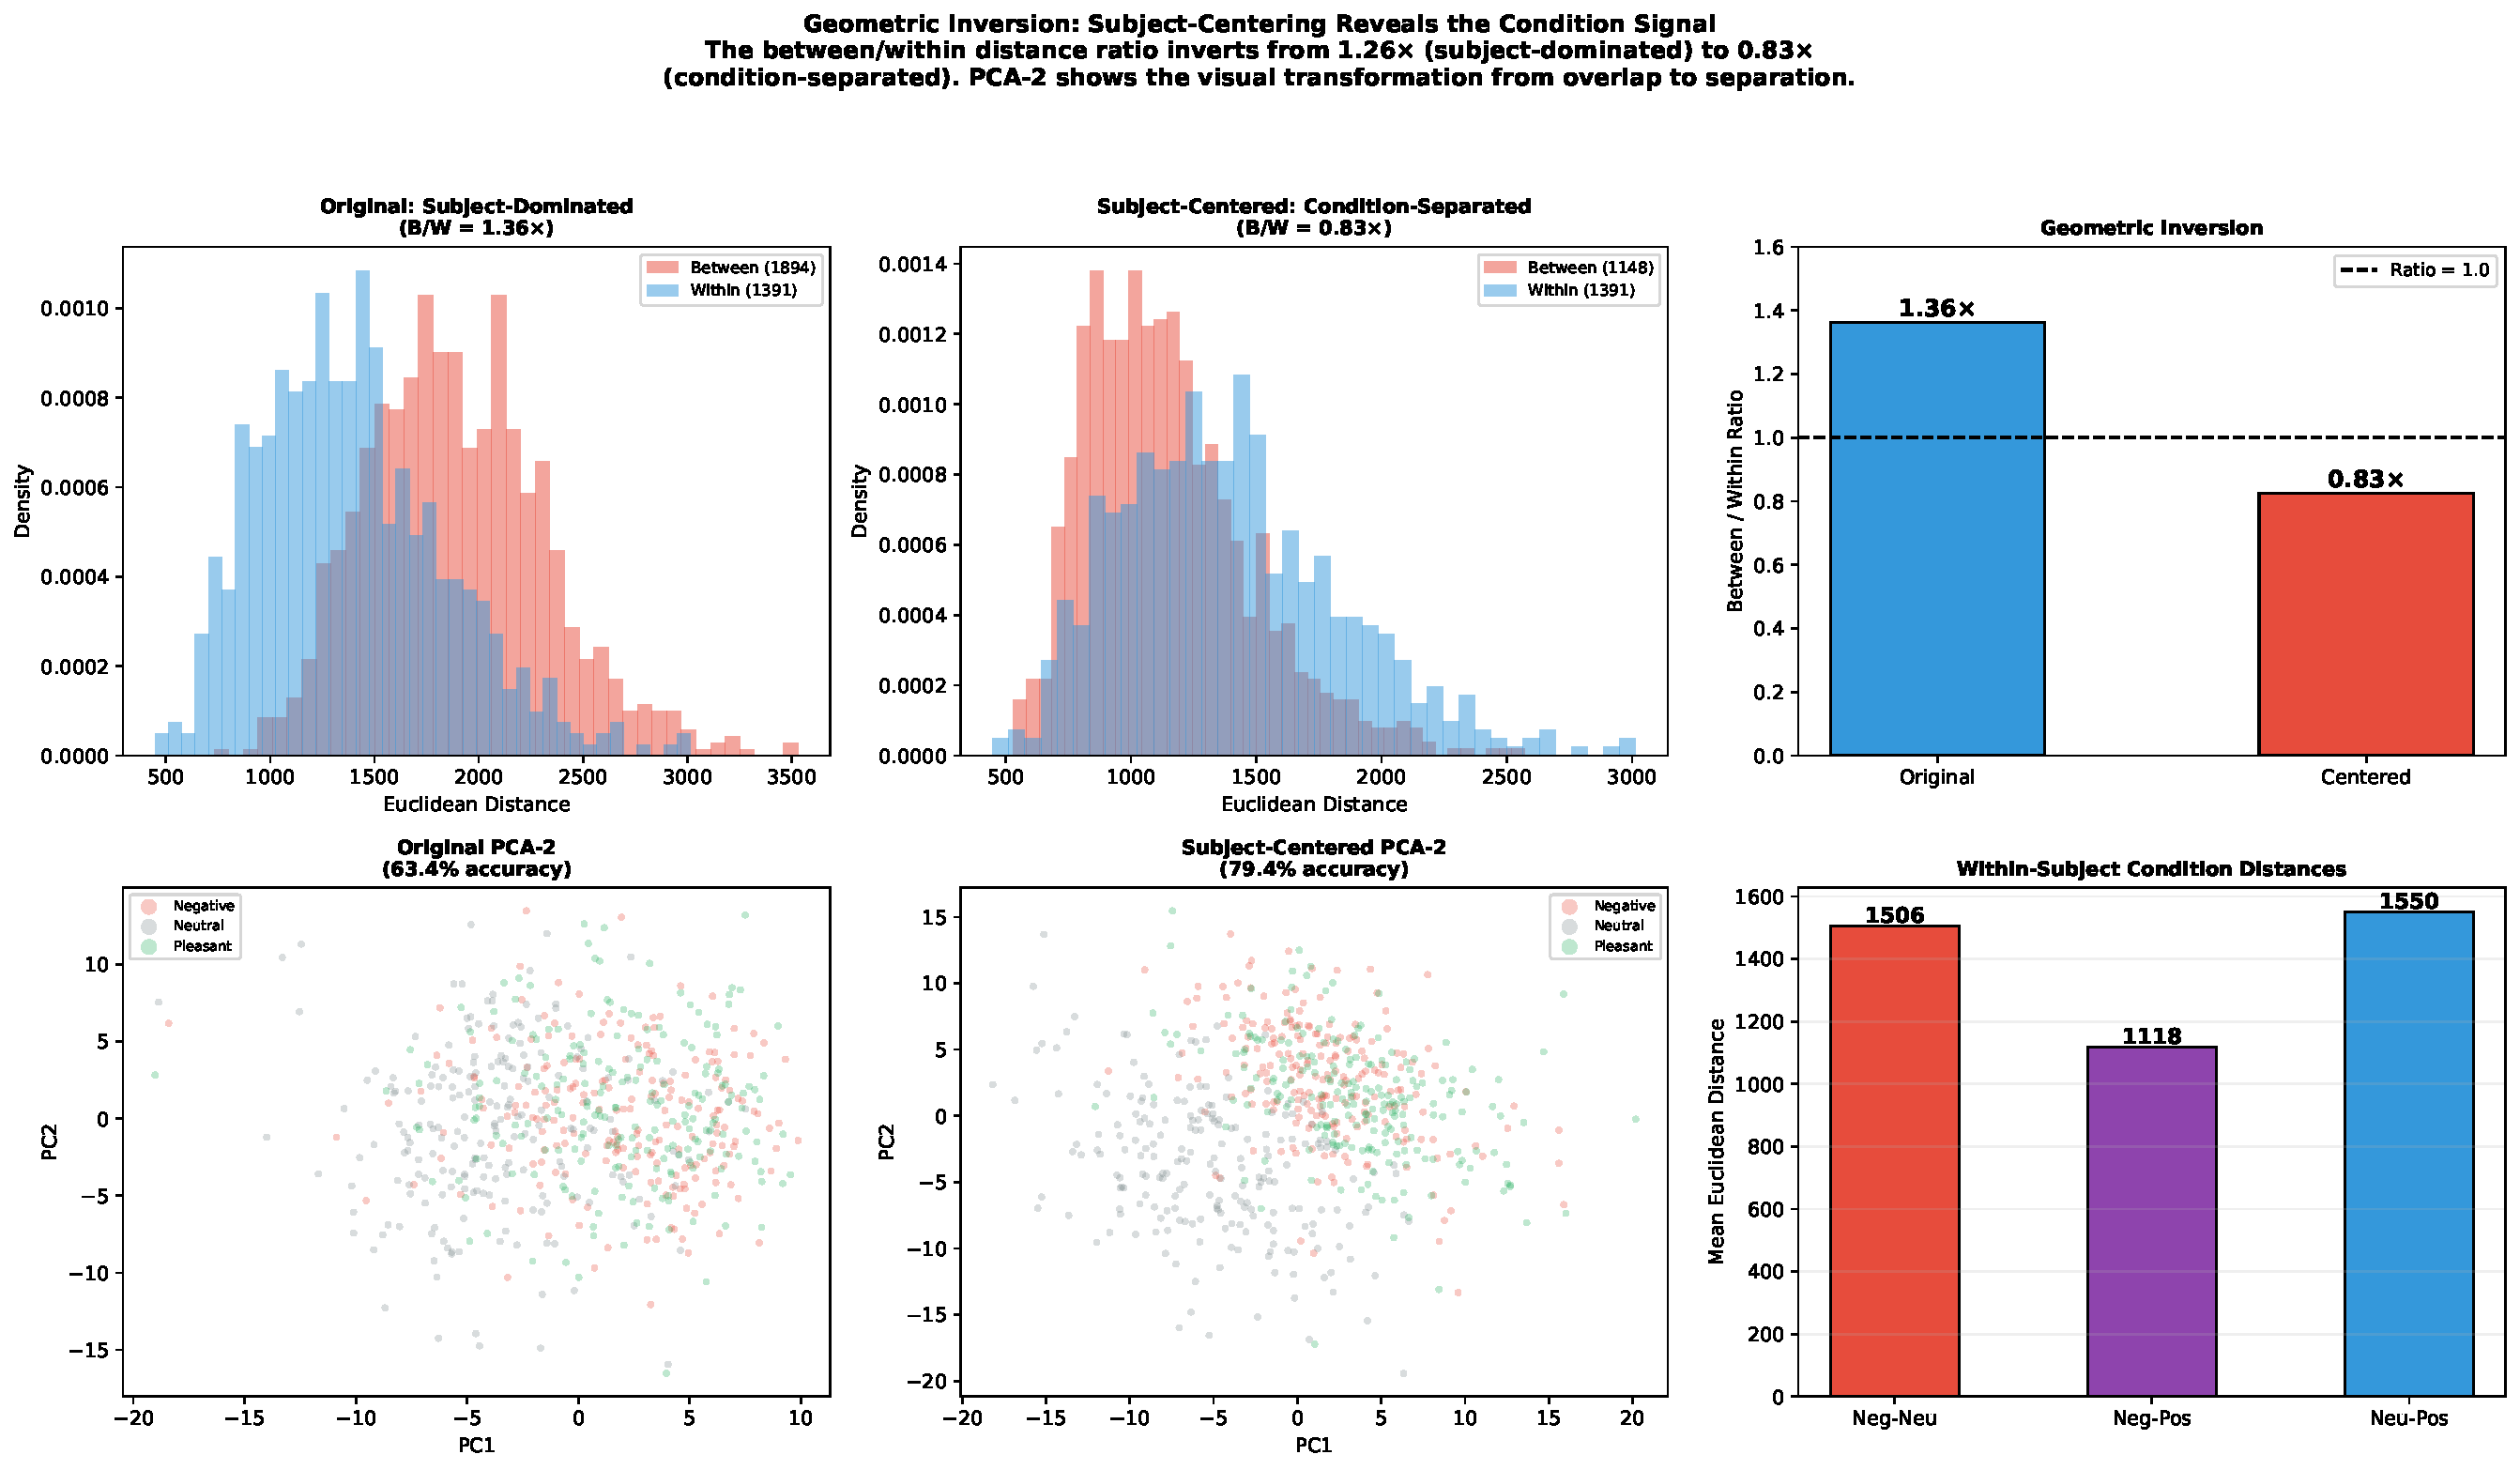
\includegraphics[width=\textwidth]{pictures/chGraphNeuralNetworks/obs14_within_between_geometry.pdf}
    \caption{Archived distance summaries before and after three-observation panel centering. The centered result is transductive, and the displayed PCA projections were fitted globally.}
    \label{fig:obs14_geometry}
\end{figure}

In the original embedding, the mean between-subject distance is $1{,}894$ and the mean within-subject cross-condition distance is $1{,}506$ (ratio $1.26$). After panel centering, the corresponding values are $1{,}148$ and $1{,}391$ (ratio $0.83$). This change is partly induced by the centering operation itself. Negative--Pleasant has the smallest displayed within-subject distance, but arousal was not modeled and is not inferred from that ordering.

The comparison shows how the chosen panel-centering operation changes the sample geometry. It does not isolate a biological nuisance component or reveal a ``true'' classification capacity. The associated $79.4\%$ value is a transductive, global-PCA legacy estimate.

\subsection{Graph Edge Stability Under Bootstrap Resampling}

Figure~\ref{fig:obs15_stability} records edge-selection frequencies across $200$ bootstrap resamples of the same subject pool. Of $561$ possible edges, $109$ are selected in more than $90\%$ of resamples, while $449$ are selected in fewer than $50\%$. These are internal selection frequencies under the same archived preprocessing, not test--retest reliability or independent-sample reproducibility.

The center panel shows that selection frequency varies by channel pair. Because the PCA-axis problem persists in every resample, frequent selection does not make an edge physiologically interpretable.

\begin{figure}[H]
    \centering
    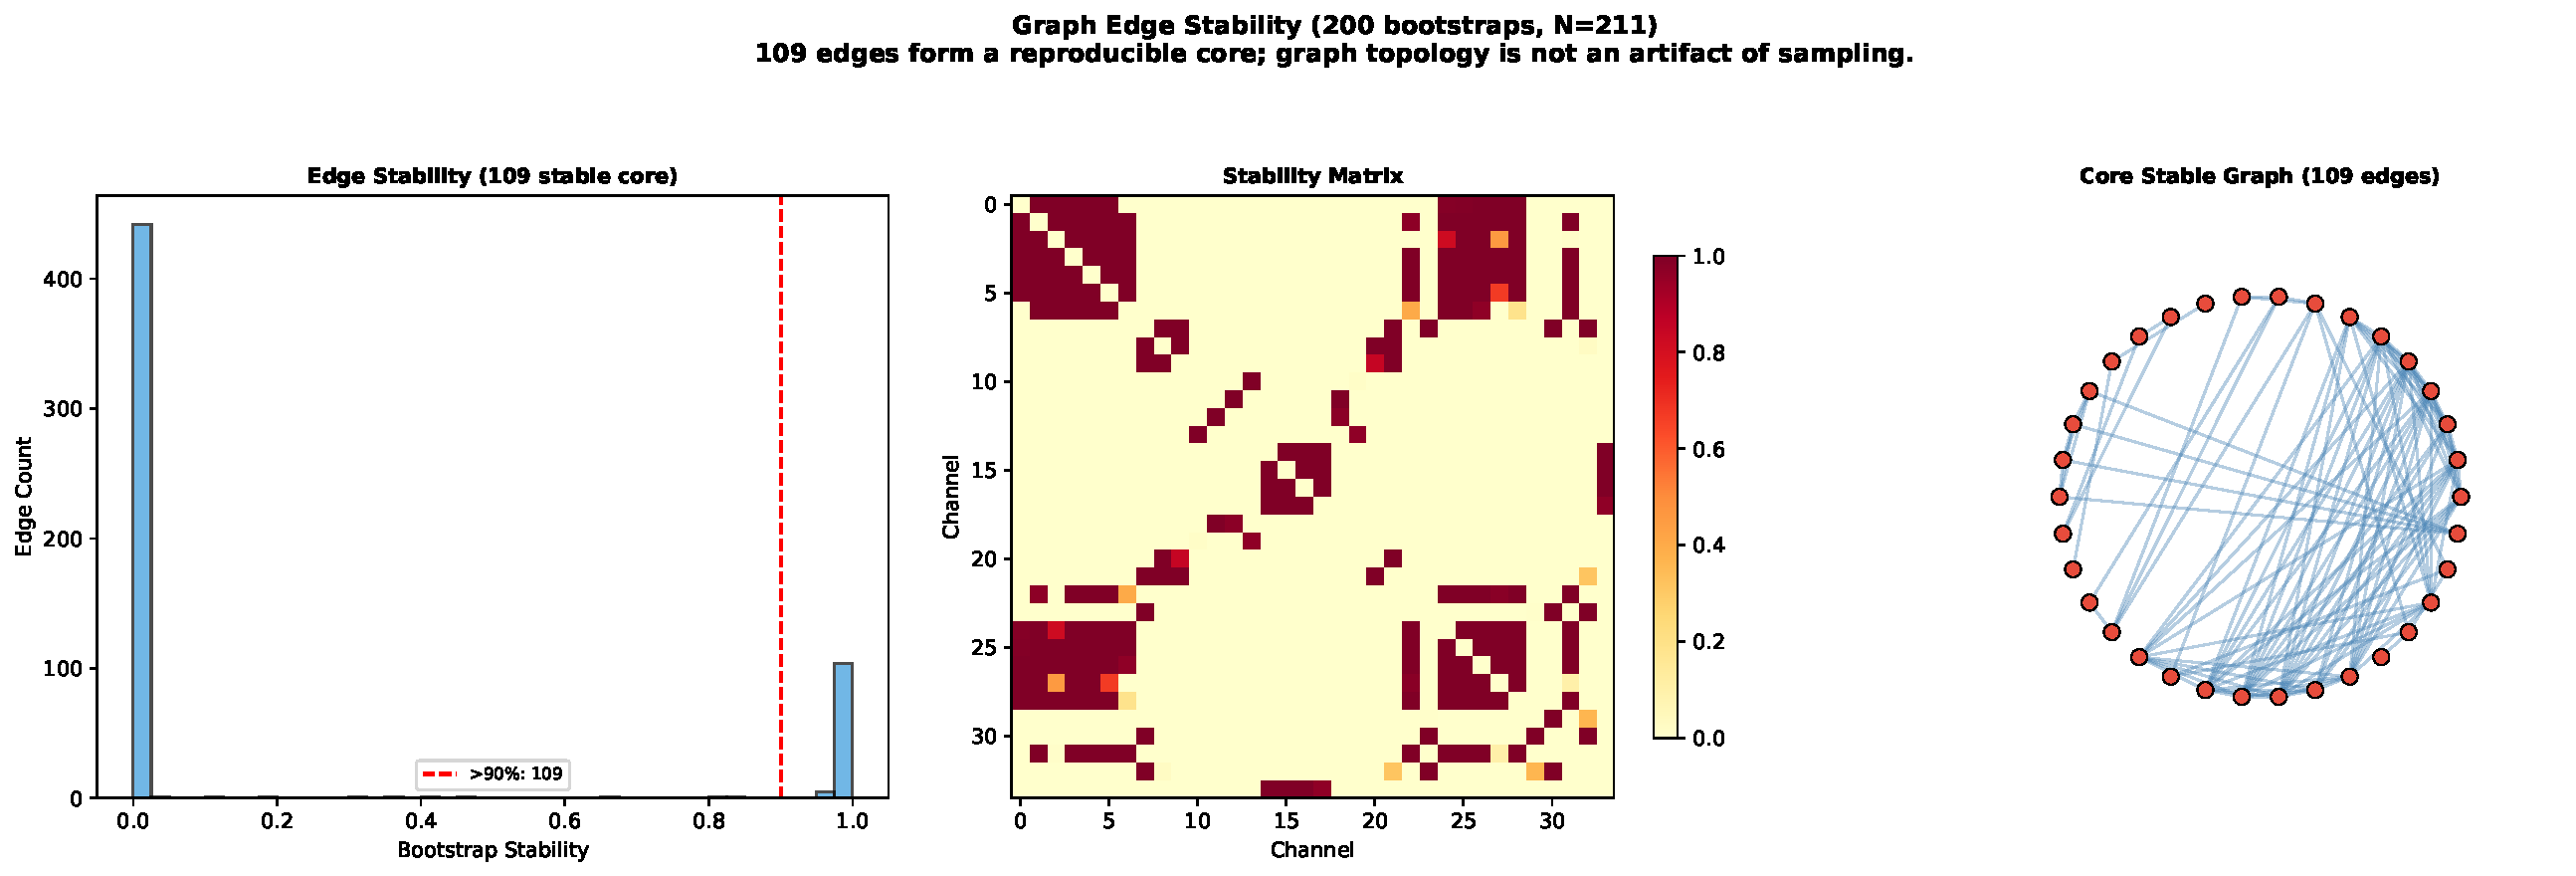
\includegraphics[width=\textwidth]{pictures/chGraphNeuralNetworks/obs15_edge_stability.pdf}
    \caption{Internal edge-selection frequencies across $200$ bootstrap resamples. Frequencies quantify stability under resampling of this cohort, not independent replication or physiological reliability.}
    \label{fig:obs15_stability}
\end{figure}

\subsection{Feature-Scale Changes Through the Pipeline}

Figure~\ref{fig:obs16_amplification} displays absolute Negative--Neutral differences after several transformations. The bars use different units and dimensional aggregations: z-scored amplitude, spike counts, sums of PCA coordinates, and centered PCA coordinates. Their heights are not comparable measures of a common signal and cannot demonstrate amplification.

The figure is retained to show the scale of each archived representation. A valid amplification comparison would require a common standardized effect or fold-wise predictive measure at every stage.

\begin{figure}[H]
    \centering
    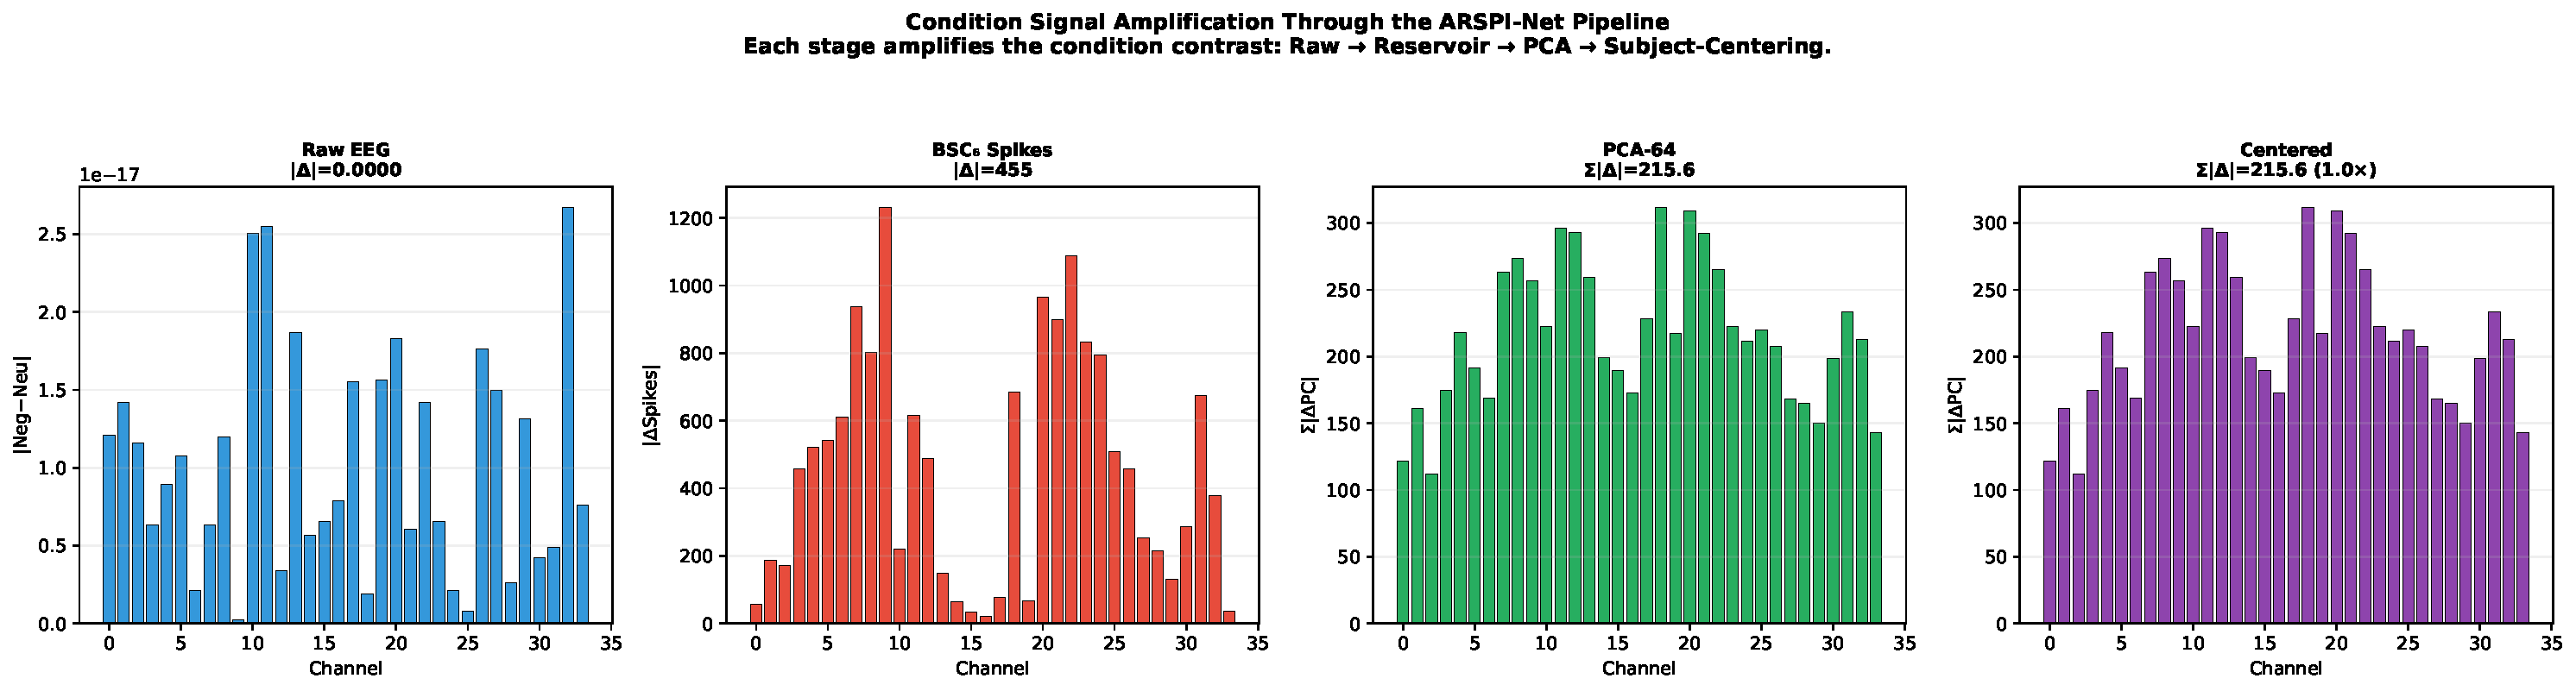
\includegraphics[width=\textwidth]{pictures/chGraphNeuralNetworks/obs16_signal_amplification.pdf}
    \caption{Archived absolute condition differences at successive pipeline stages. Bar heights use incompatible units and aggregations and therefore must not be compared as amplification factors.}
    \label{fig:obs16_amplification}
\end{figure}

\subsection{Graph Laplacian Spectral Characterization}

The Laplacian $\mathbf{L}=\mathbf{D}-\mathbf{A}$ summarizes the archived thresholded graph, and its eigenspectrum determines the action of linear polynomial filters on that graph. Figure~\ref{fig:obs17_spectral} records these mathematical properties; it does not establish properties of an anatomical electrode network.

\begin{figure}[H]
    \centering
    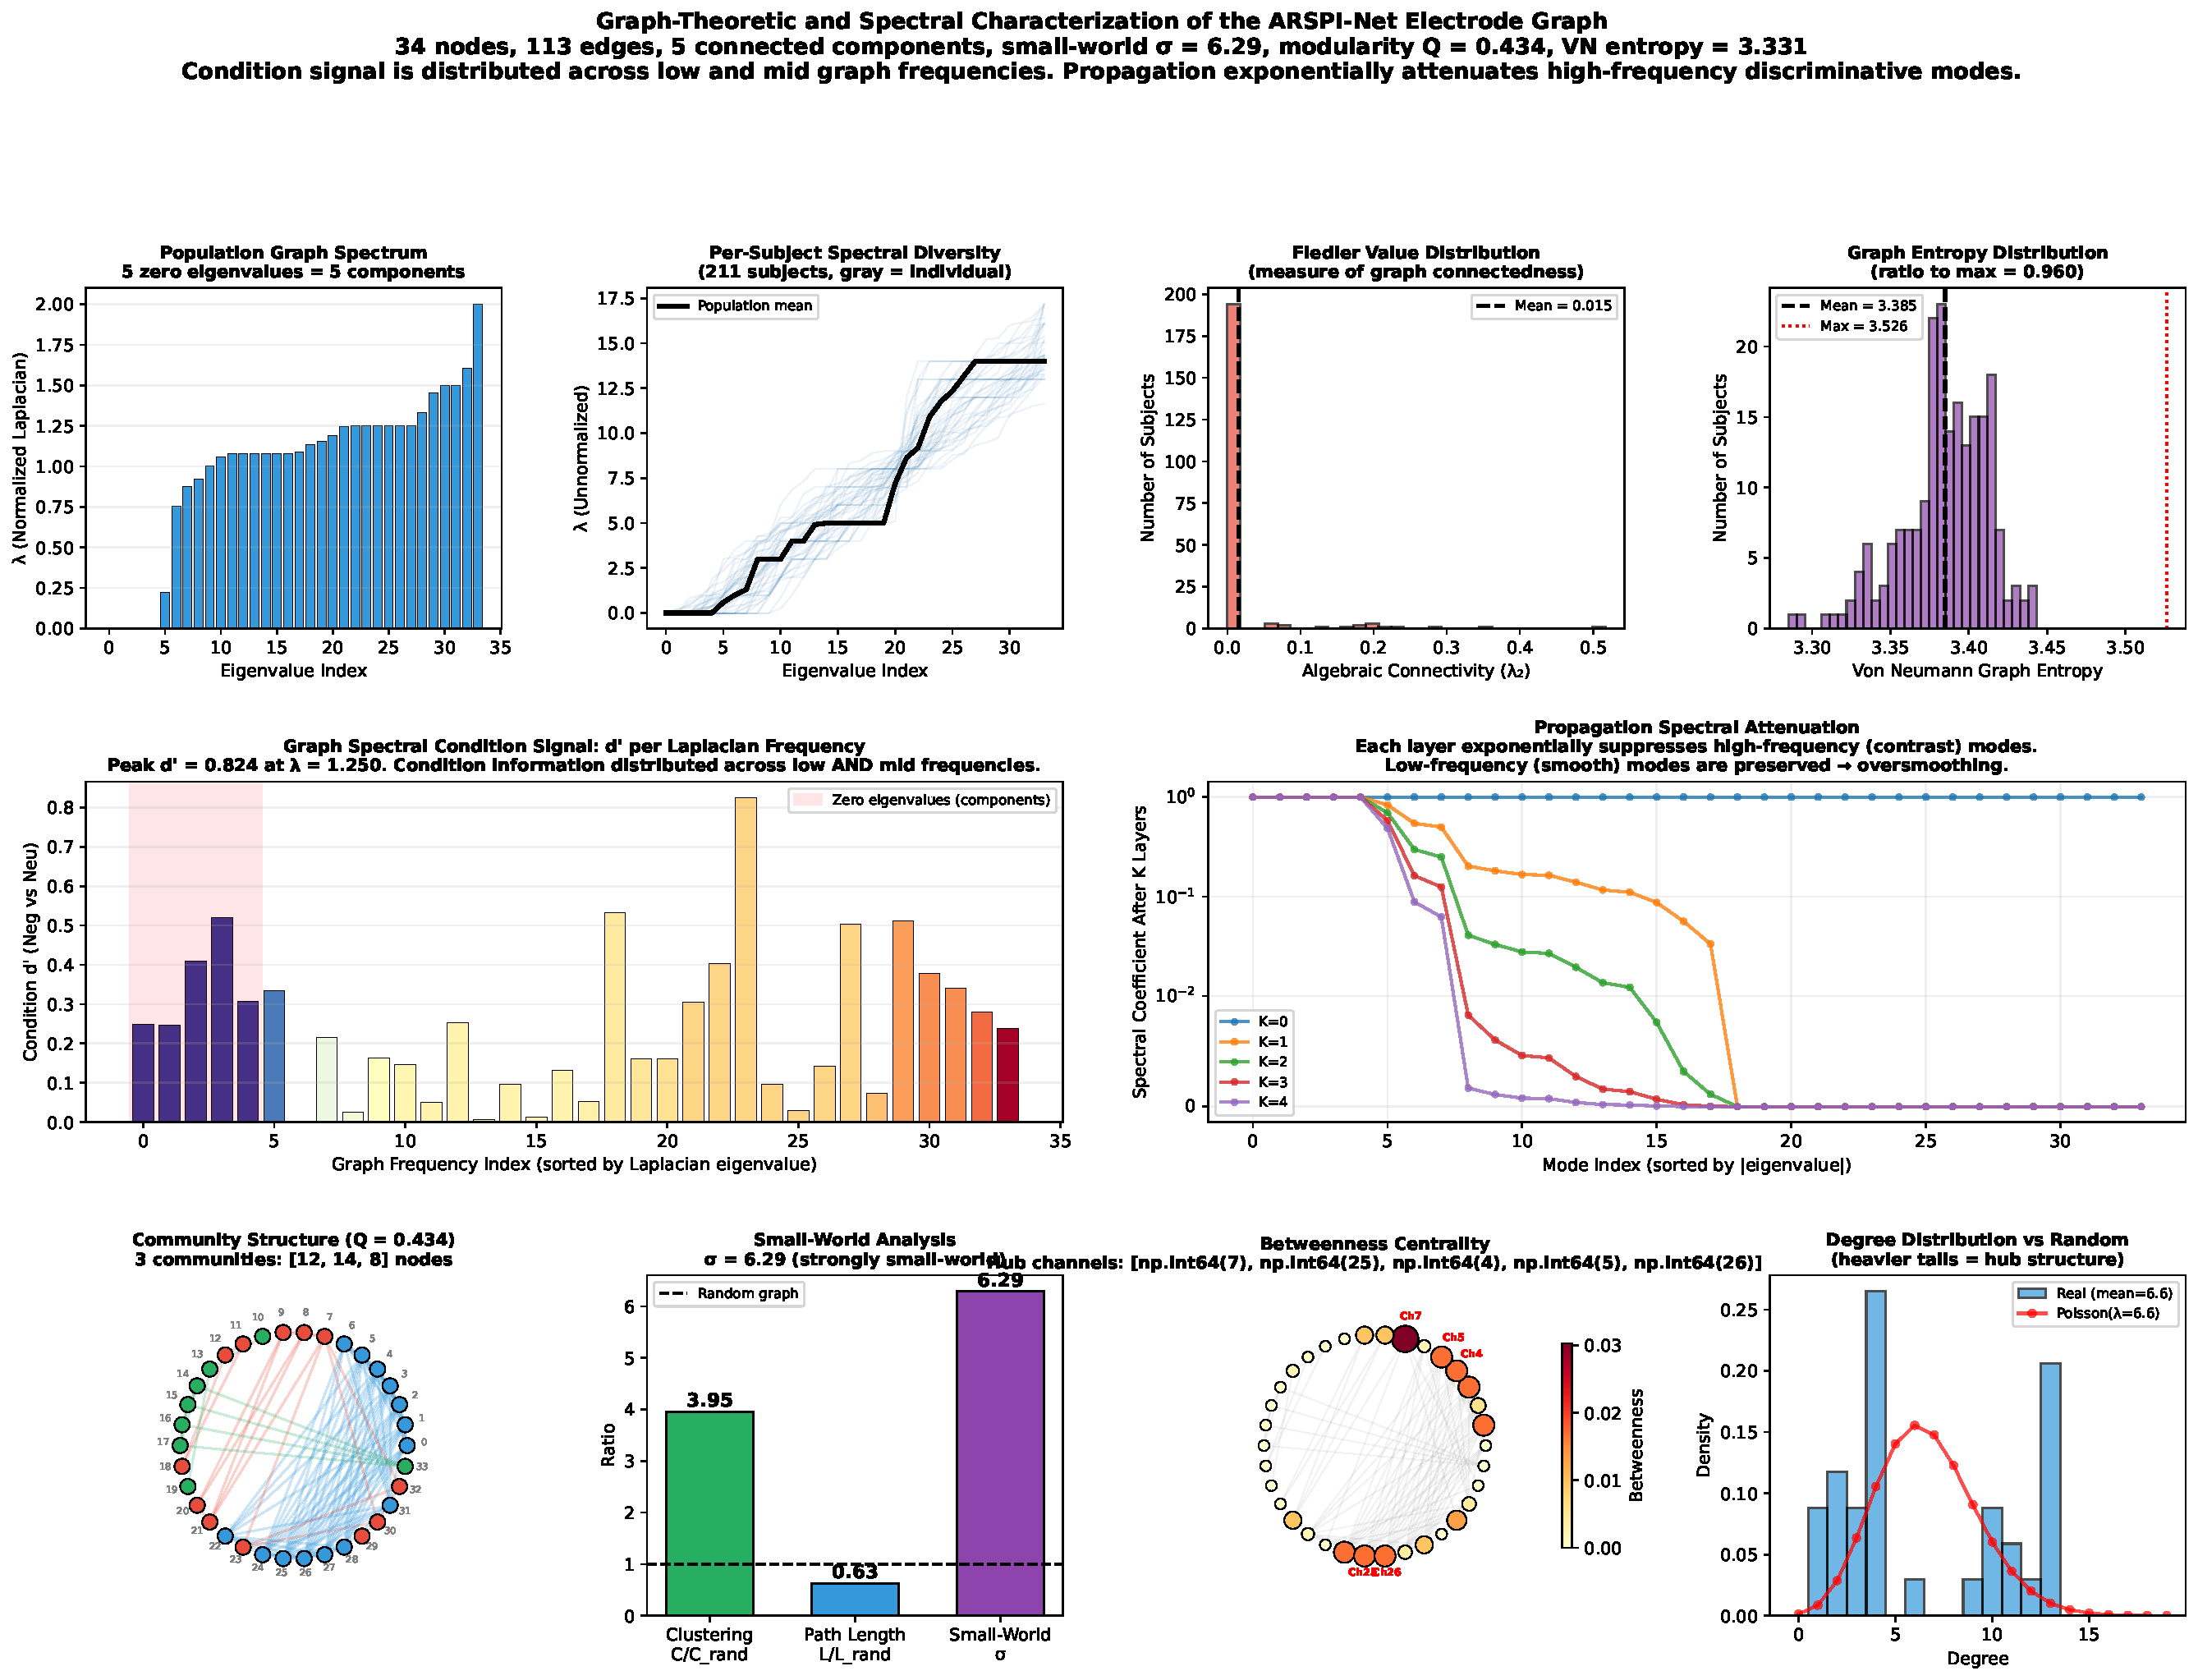
\includegraphics[width=\textwidth]{pictures/chGraphNeuralNetworks/obs17_spectral_analysis.pdf}
    \caption{Spectral summaries of the archived thresholded similarity graph. Values inherit the noncommensurate-PCA-basis limitation and have no anatomical interpretation.}
    \label{fig:obs17_spectral}
\end{figure}

The normalized Laplacian of the population-average graph has five zero eigenvalues, corresponding to five connected components at the $20\%$ threshold. Its Fiedler value is therefore effectively zero. Across participant-specific graphs, the displayed Fiedler value is $0.015 \pm 0.061$. The von Neumann graph-entropy calculation gives $3.331$, or $0.945$ of $\ln 34=3.526$; the participant-specific mean is $3.385\pm0.028$. These are properties of the legacy thresholded matrices, not evidence about robustness to perturbations or neural-network complexity.

The archived graph-Fourier panel displays Negative--Neutral d$'$ values across graph modes. Linear propagation attenuates modes according to their adjacency eigenvalues, but the panel does not show that attenuated modes uniquely carry condition information or that standardized detectability must fall.

After $K$ layers of normalized linear propagation, the $i$th mode is multiplied by $\mu_i^K$. Modes with $|\mu_i|<0.2$ retain less than $4\%$ of their squared amplitude after two layers. This algebraic attenuation is reversible only if the operator is invertible and numerically stable; it should not be equated with a measured loss of mutual information.

\subsection{Archived Small-World and Community Summaries}

The archived thresholded graph has a high clustering-to-random ratio and short paths within its largest component. Figure~\ref{fig:obs20_topology} summarizes these graph-theoretic values.

\begin{figure}[H]
    \centering
    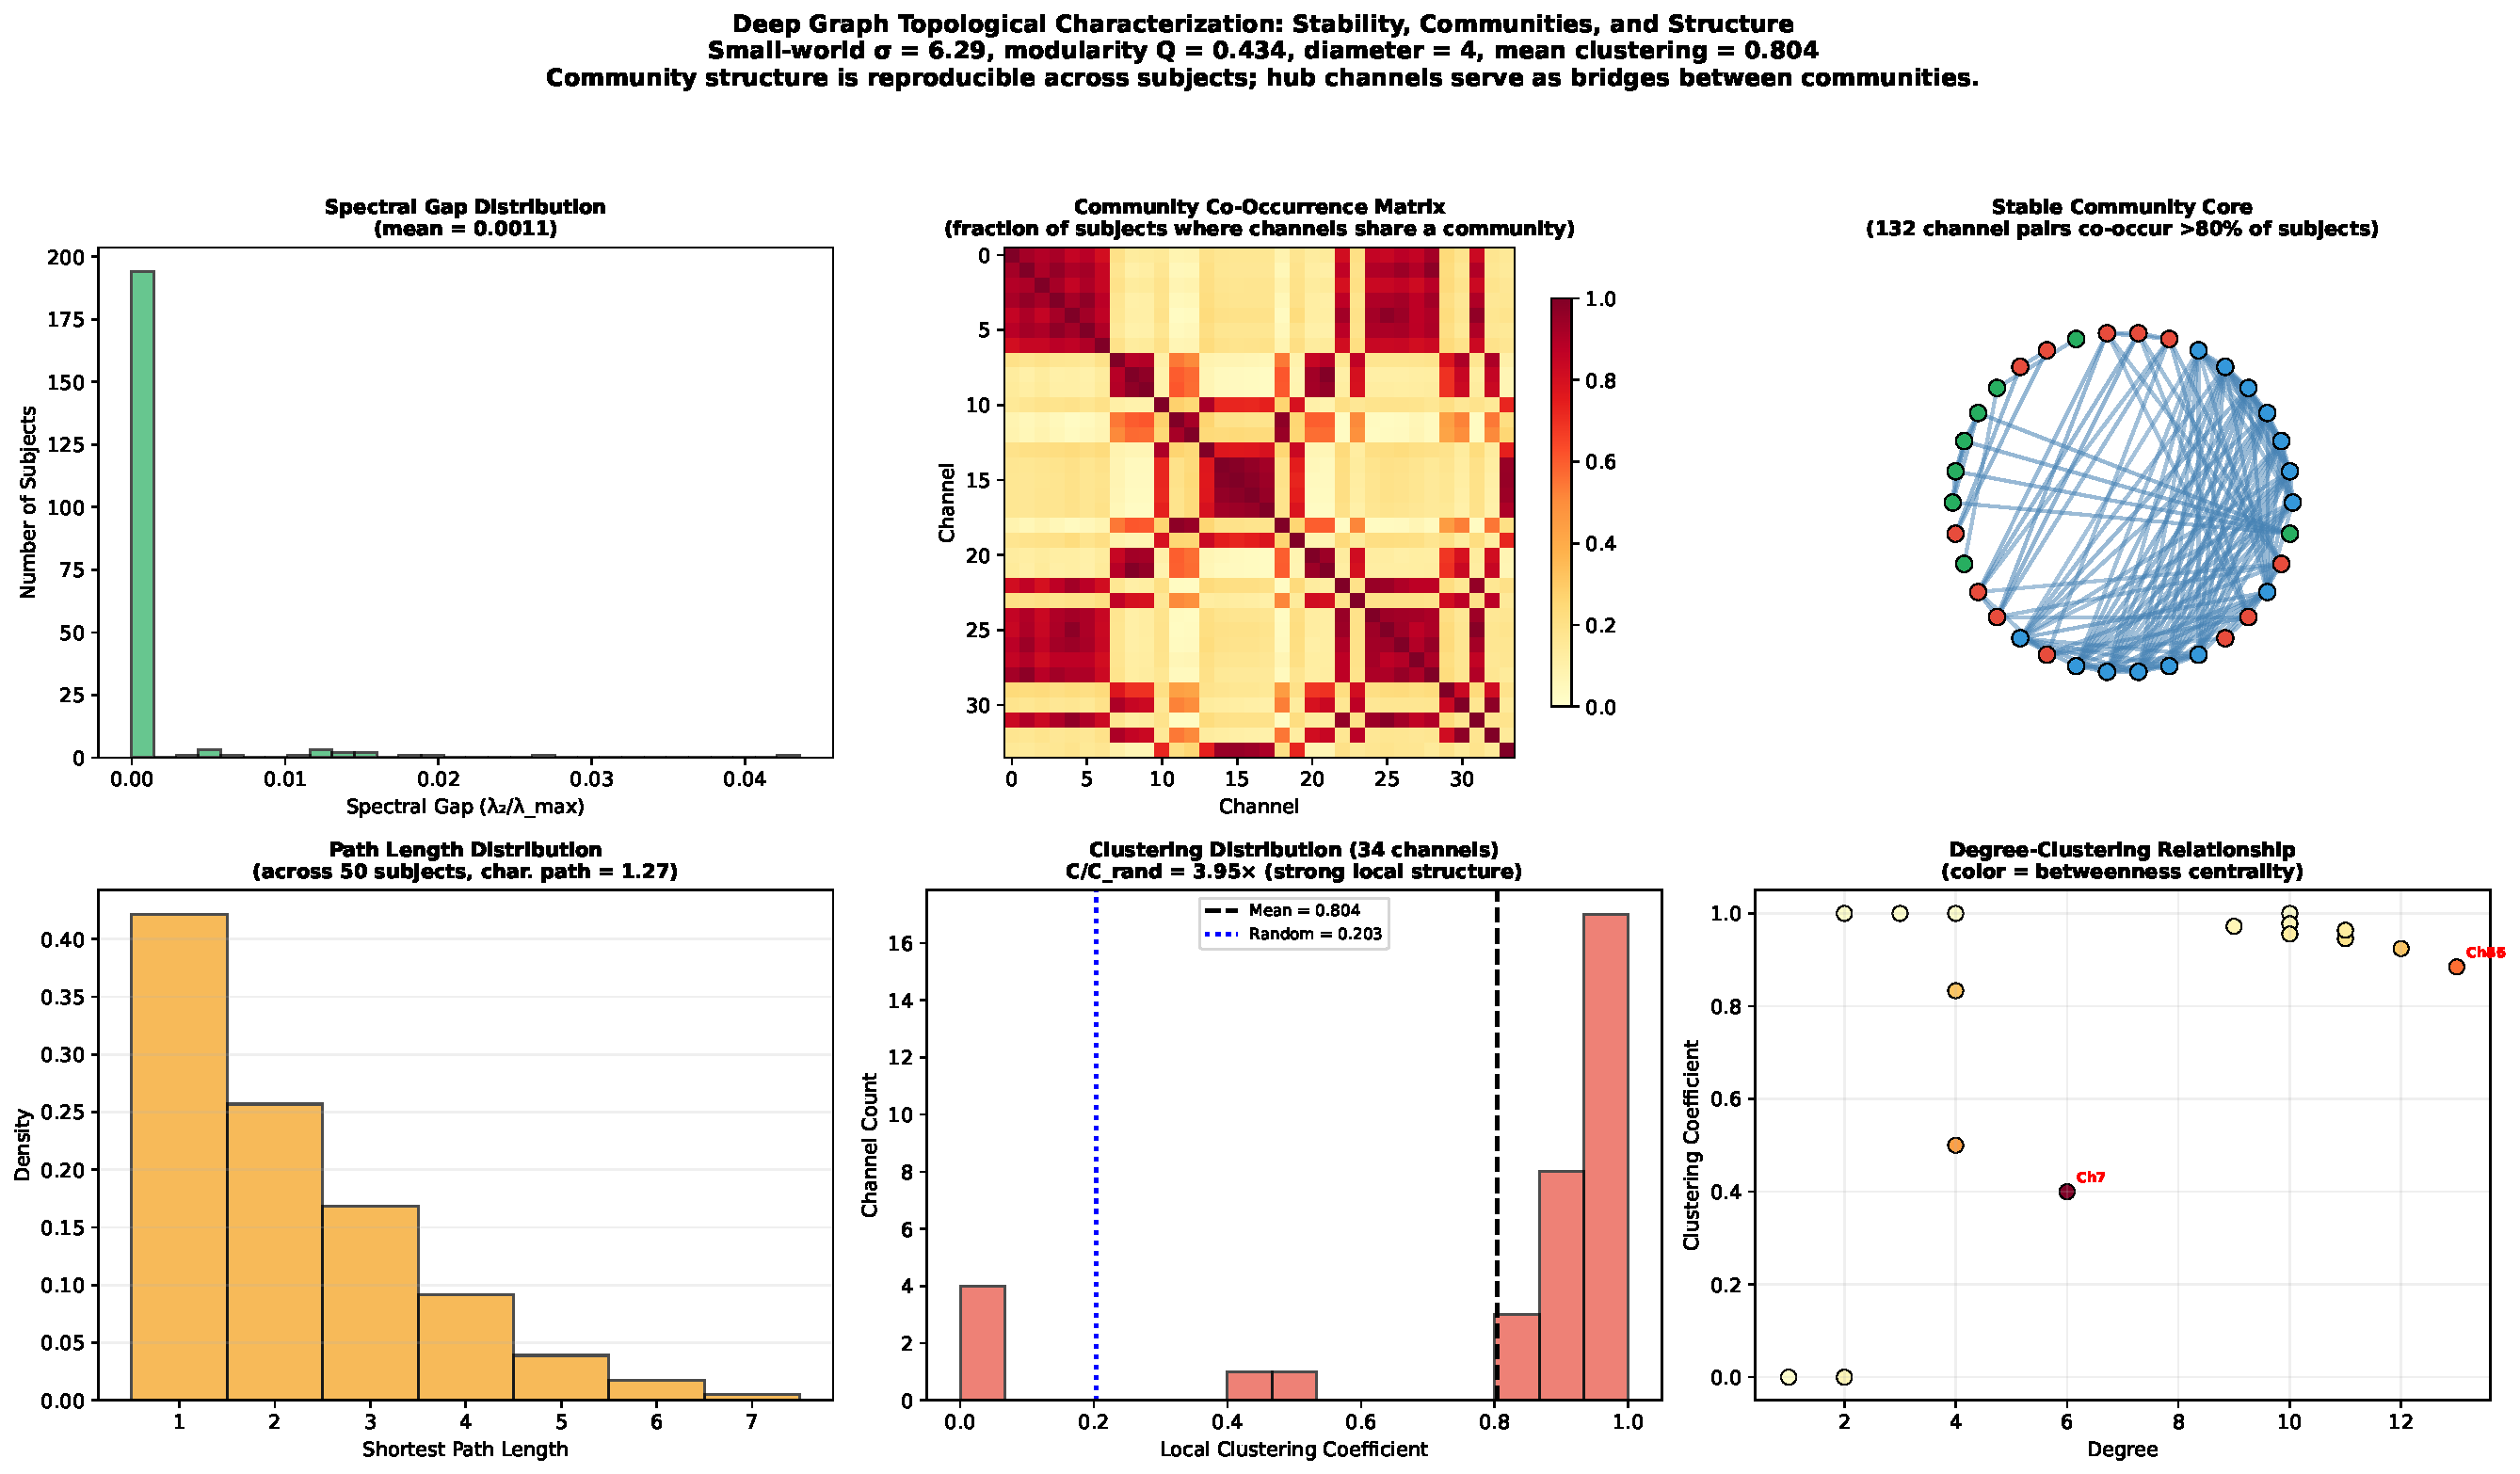
\includegraphics[width=\textwidth]{pictures/chGraphNeuralNetworks/obs20_deep_topology.pdf}
    \caption{Archived graph summaries. Top: spectral-gap distribution, community co-occurrence among channel indices, and pairs with more than $80\%$ co-occurrence. Bottom: largest-component path lengths, clustering relative to the selected degree-matched random-graph null, and degree--clustering values. Labels such as Ch7 and Ch25 are channel indices without anatomical assignments.}
    \label{fig:obs20_topology}
\end{figure}

The clustering coefficient is $3.95\times$ that of the selected degree-matched random graphs ($0.804$ versus $0.203$), and the reported largest-component path length is $1.27$ versus $2.01$, yielding $\sigma=6.29$. This value depends on the threshold, component convention, and random-graph null. It characterizes the legacy similarity graph and does not imply efficient neural communication \cite{rubinov_complex_2010}.

Hierarchical clustering produces three communities with modularity $Q=0.434$, and some channel-index pairs co-occur in more than $80\%$ of within-cohort resamples. These are algorithm-dependent groups of unlabeled indices. Terms such as ``community'' and ``bridge'' describe graph roles only and cannot be mapped to brain regions in the present data.

\subsection{Per-Subject Graph Topology Gallery}

Figure~\ref{fig:obs18_gallery} displays the archived graphs for $20$ randomly selected participants. Their component counts and clustering values vary. The exploratory clinical analyses below test selected group comparisons but do not establish that group effects rise above this variability.

\begin{figure}[H]
    \centering
    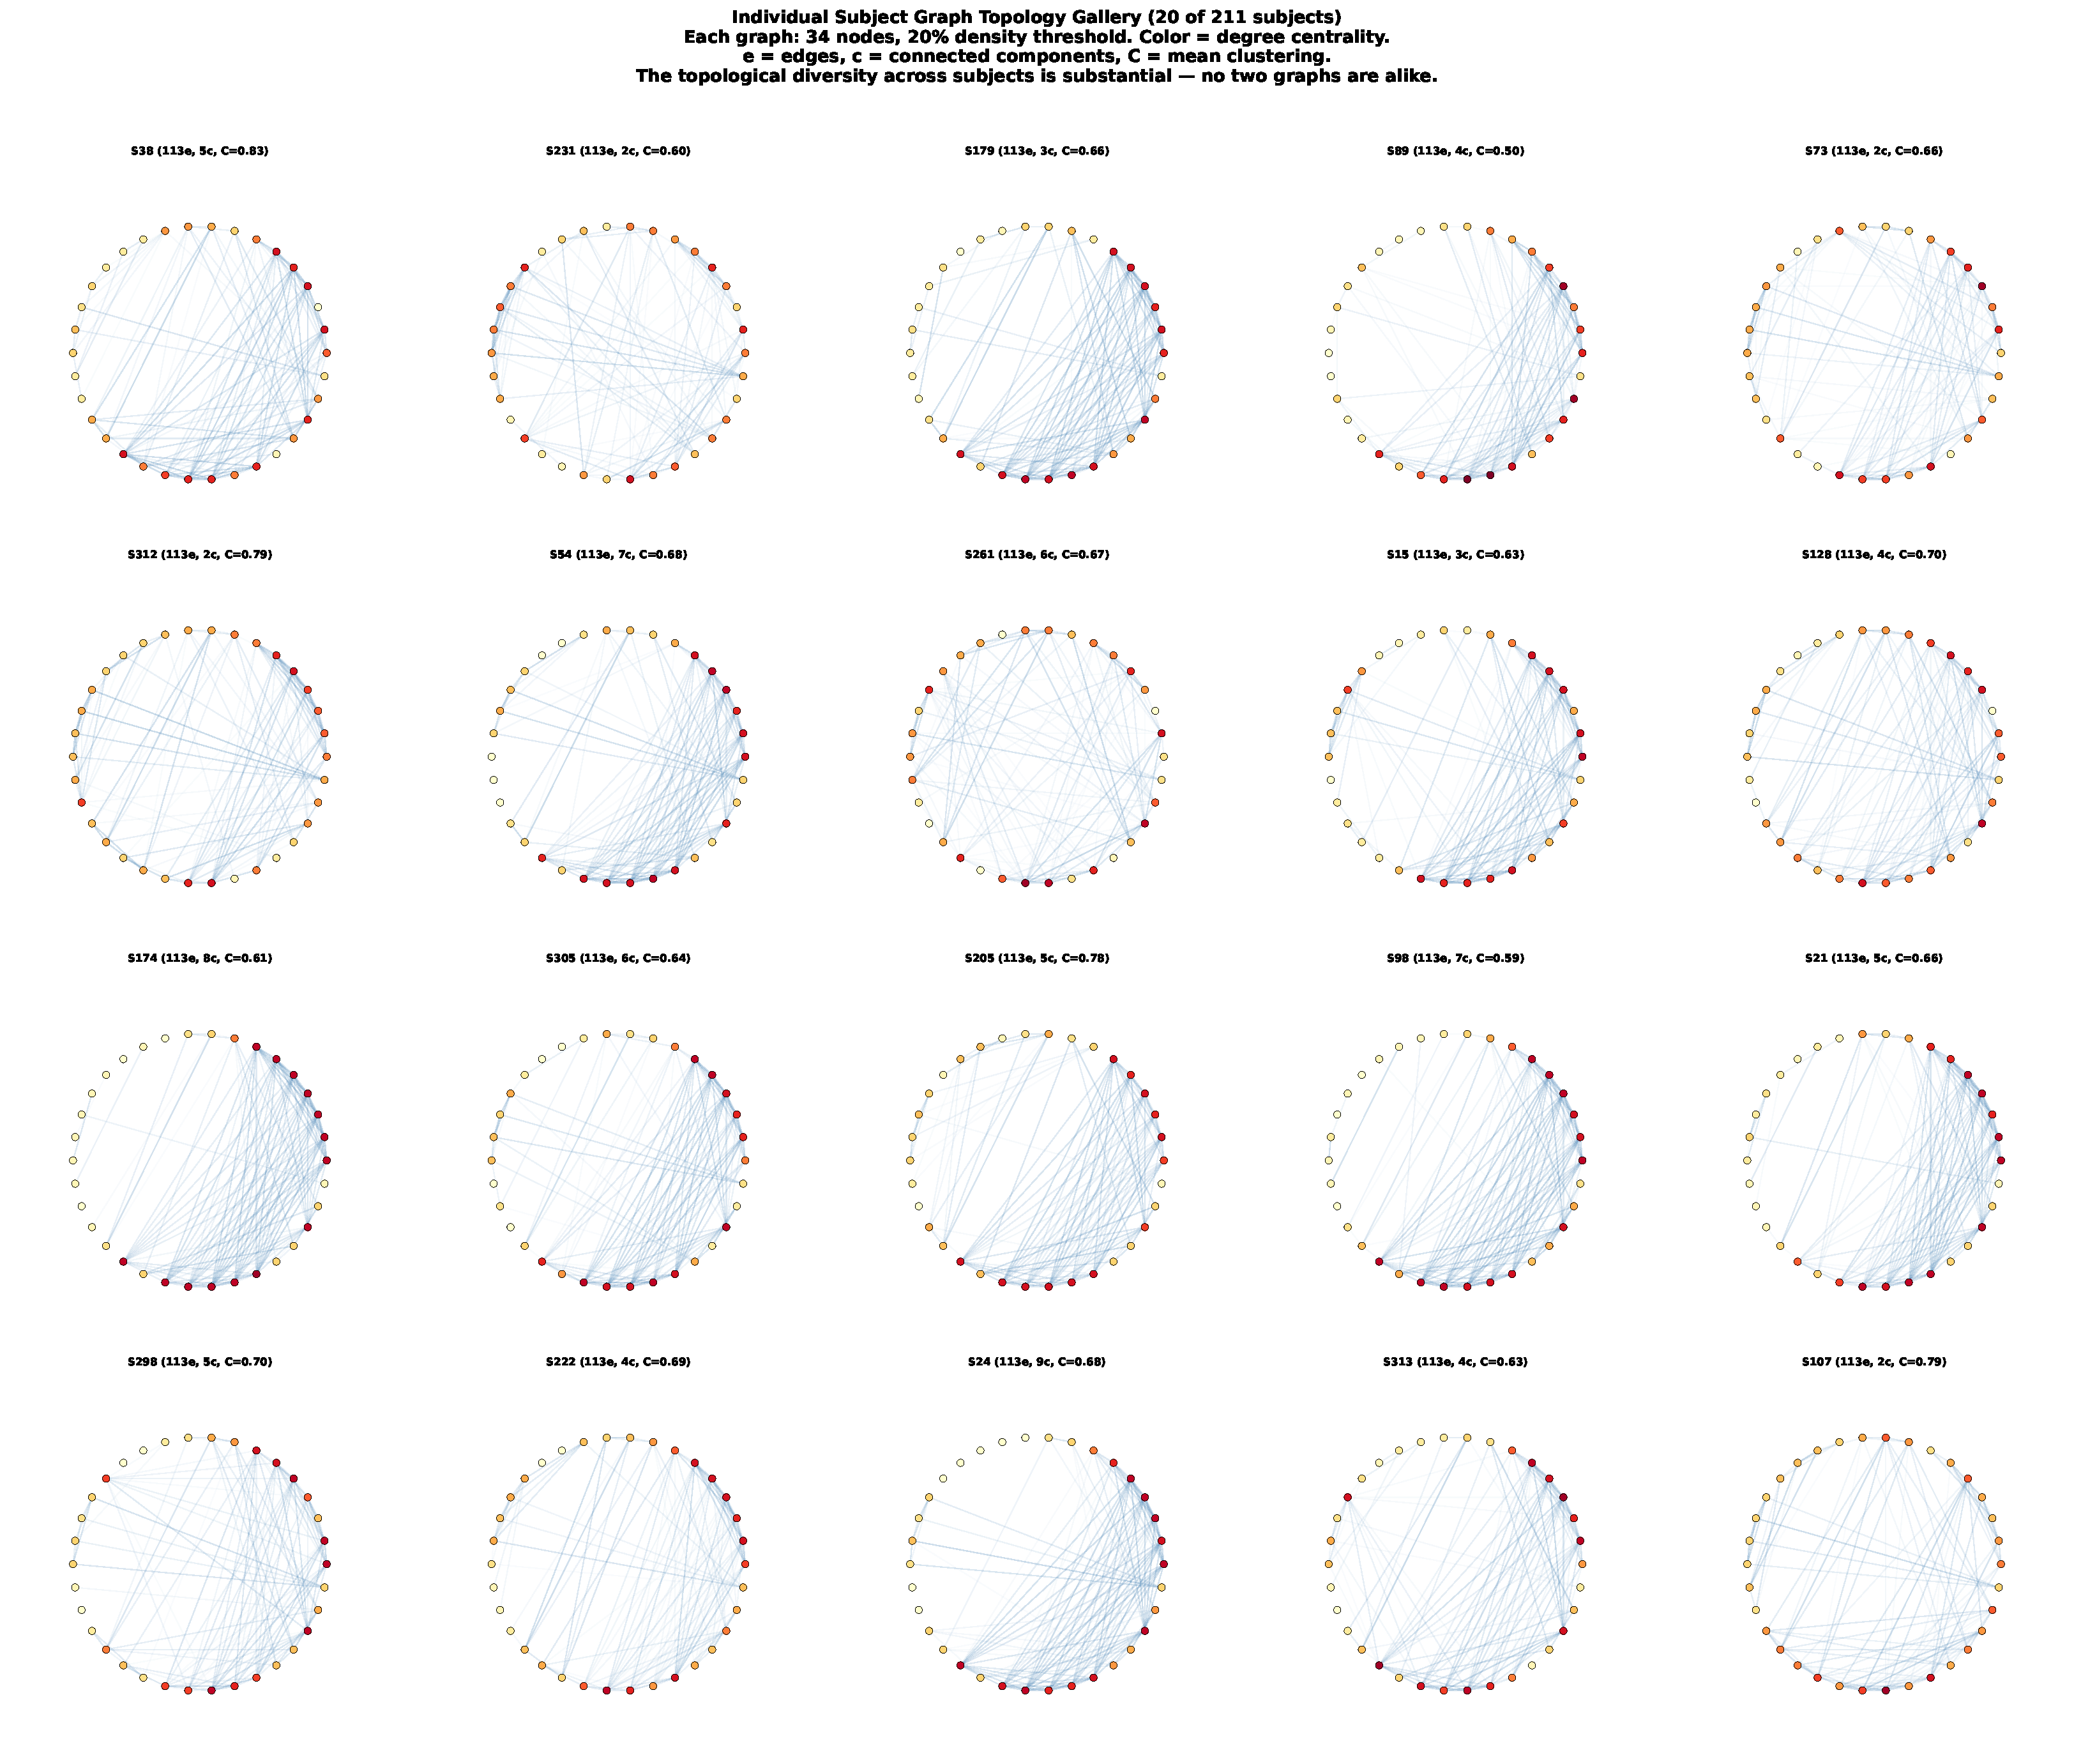
\includegraphics[width=\textwidth]{pictures/chGraphNeuralNetworks/obs18_subject_gallery.pdf}
    \caption{Archived graph gallery for $20$ of $211$ participants. Each graph has $34$ nodes and uses the $20\%$ density threshold. Node color shows degree centrality; $e$ denotes edges, $c$ connected components, and $\bar{C}$ mean clustering.}
    \label{fig:obs18_gallery}
\end{figure}

\subsection{Condition-Specific Graph Spectral Analysis}

Figure~\ref{fig:obs19_cond_spectral} compares the archived condition-specific graph spectra. The displayed eigenvalues and entropy summaries differ slightly by condition. No prespecified inferential test is reported for the full spectral family, and a higher graph entropy is not interpreted as greater physiological ``structural complexity.''

\begin{figure}[H]
    \centering
    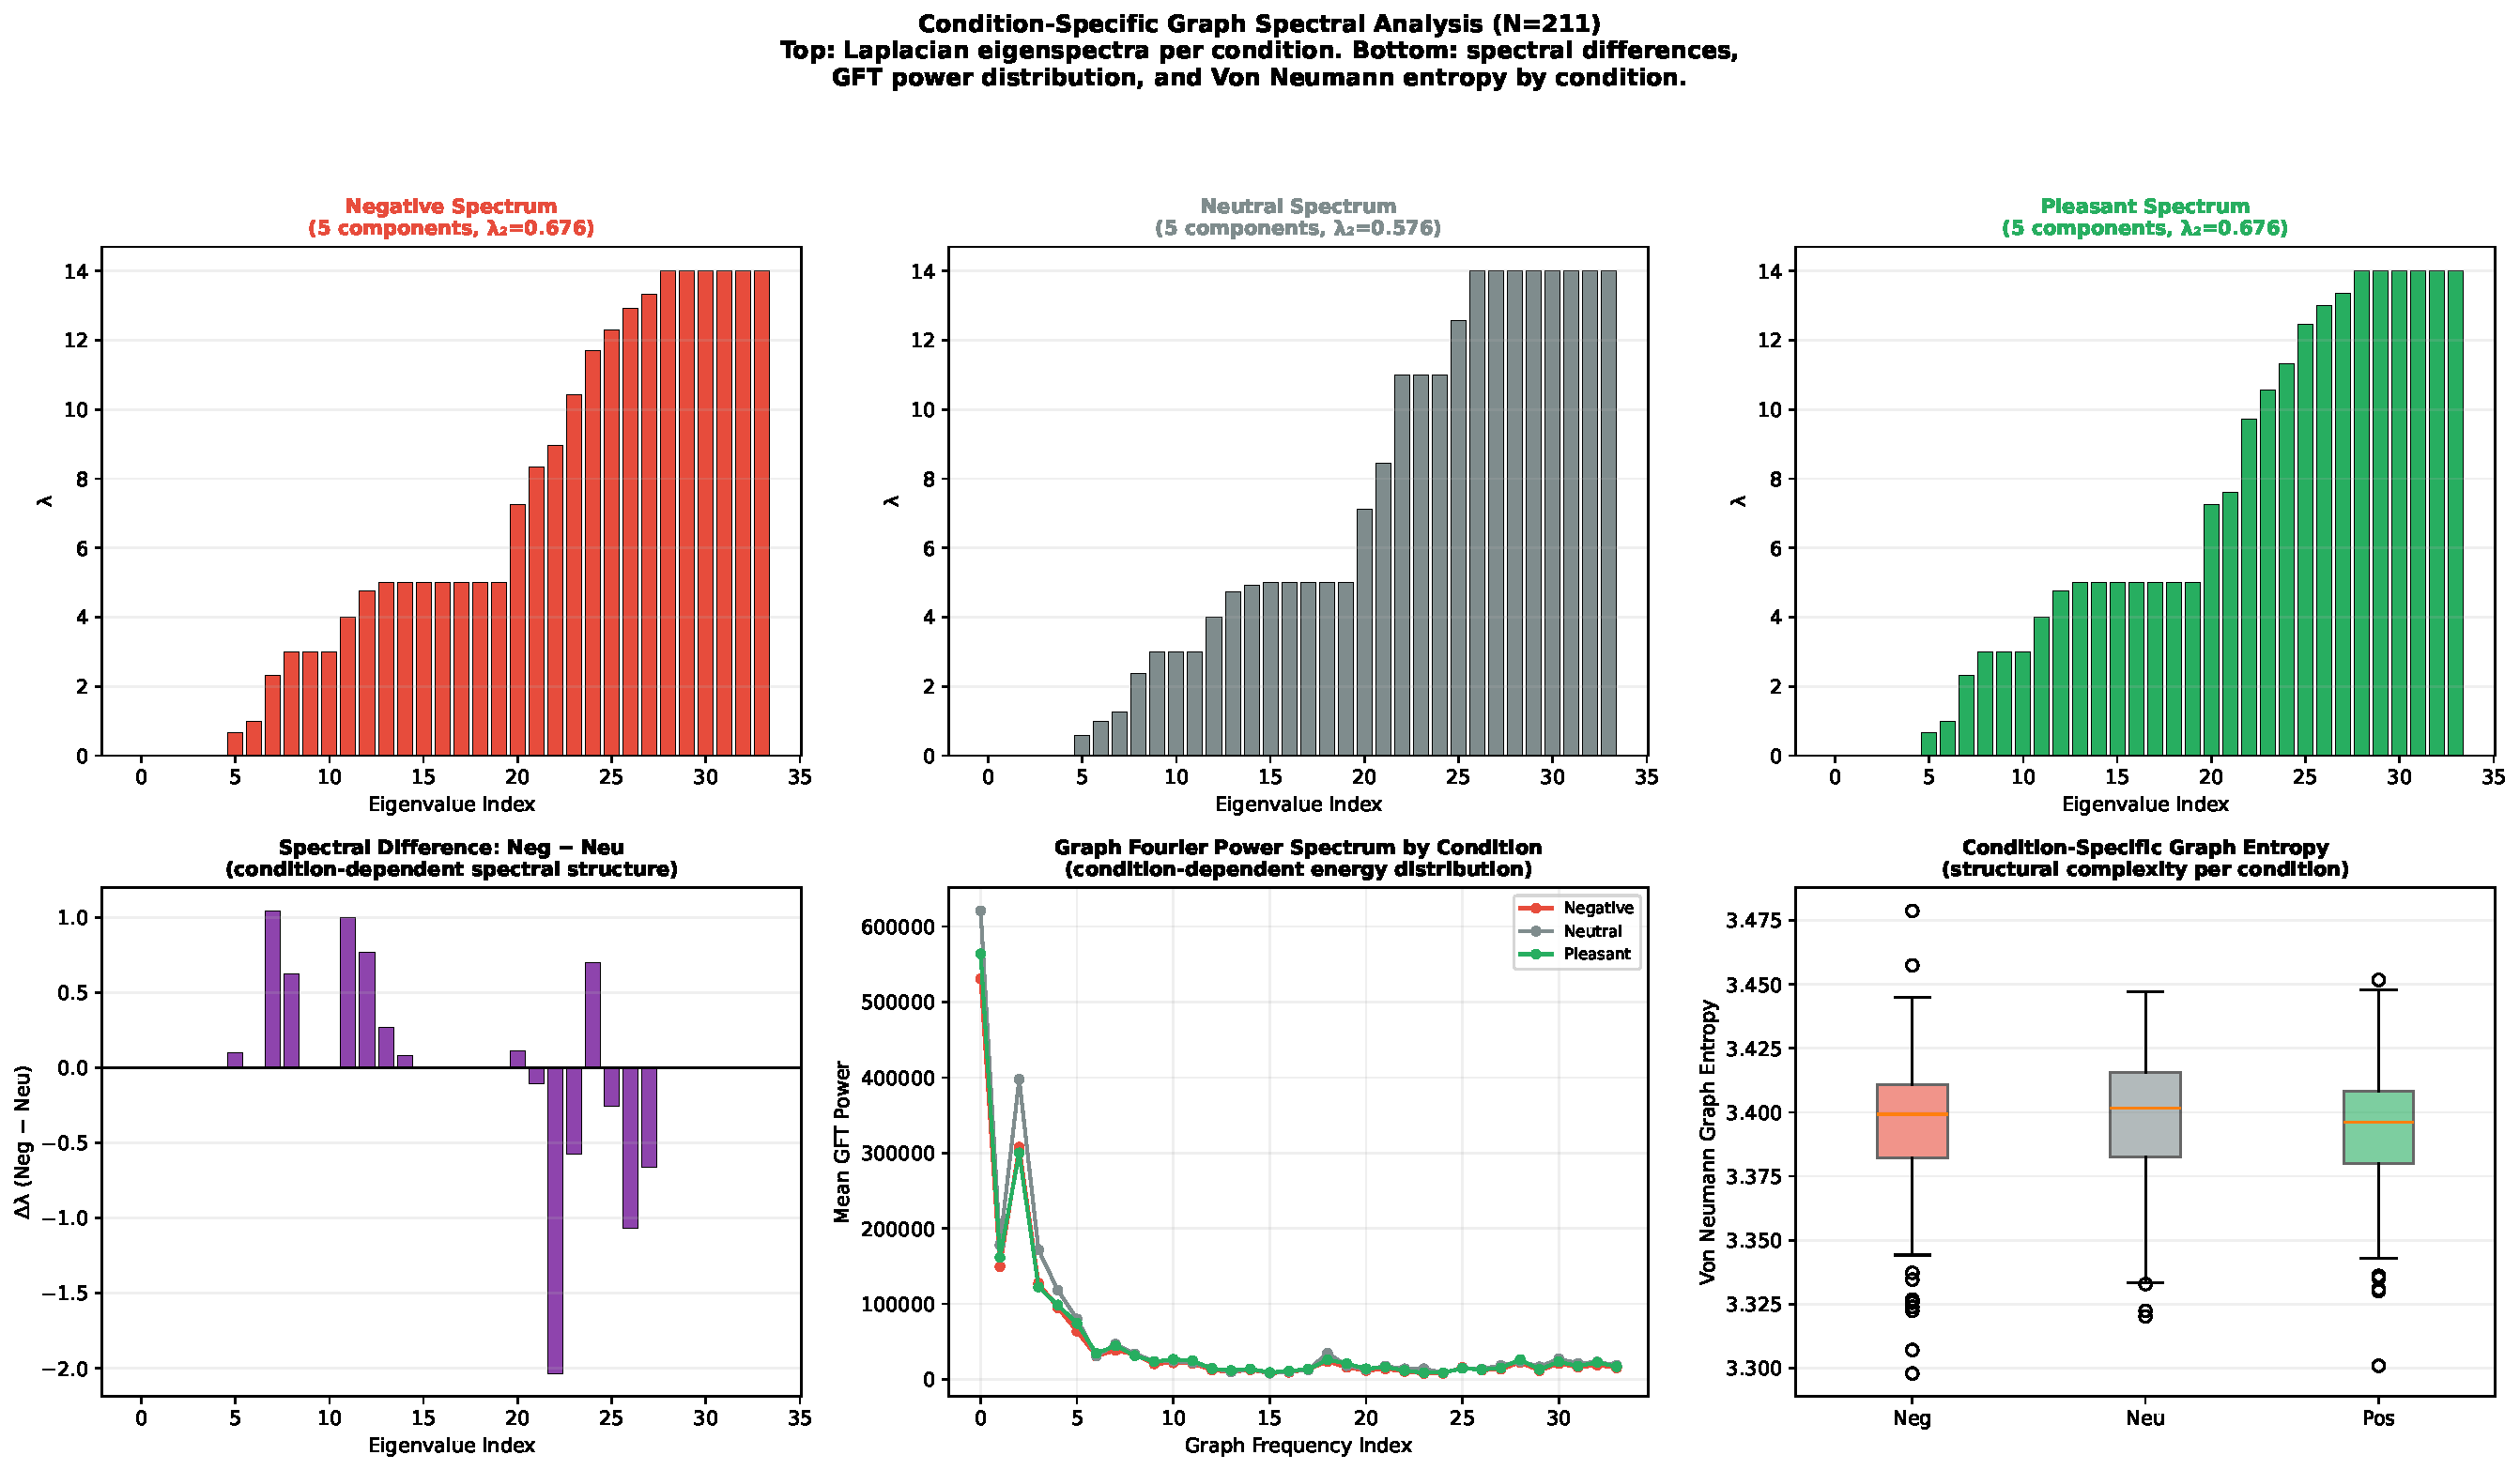
\includegraphics[width=\textwidth]{pictures/chGraphNeuralNetworks/obs19_condition_spectral.pdf}
    \caption{Archived condition-specific spectral summaries. Differences are descriptive and inherit the graph-construction limitations described in the text.}
    \label{fig:obs19_cond_spectral}
\end{figure}

\subsection{Grand-Average ERPs: The Condition Signal}

Figure~\ref{fig:obs08_erps} displays grand-average waveforms for four channel indices. Negative-minus-Neutral differences are small relative to the z-scored waveform range. Without verified electrode labels, component-specific channels, and prespecified windows, the figure is not used to claim an LPP effect.

\begin{figure}[H]
    \centering
    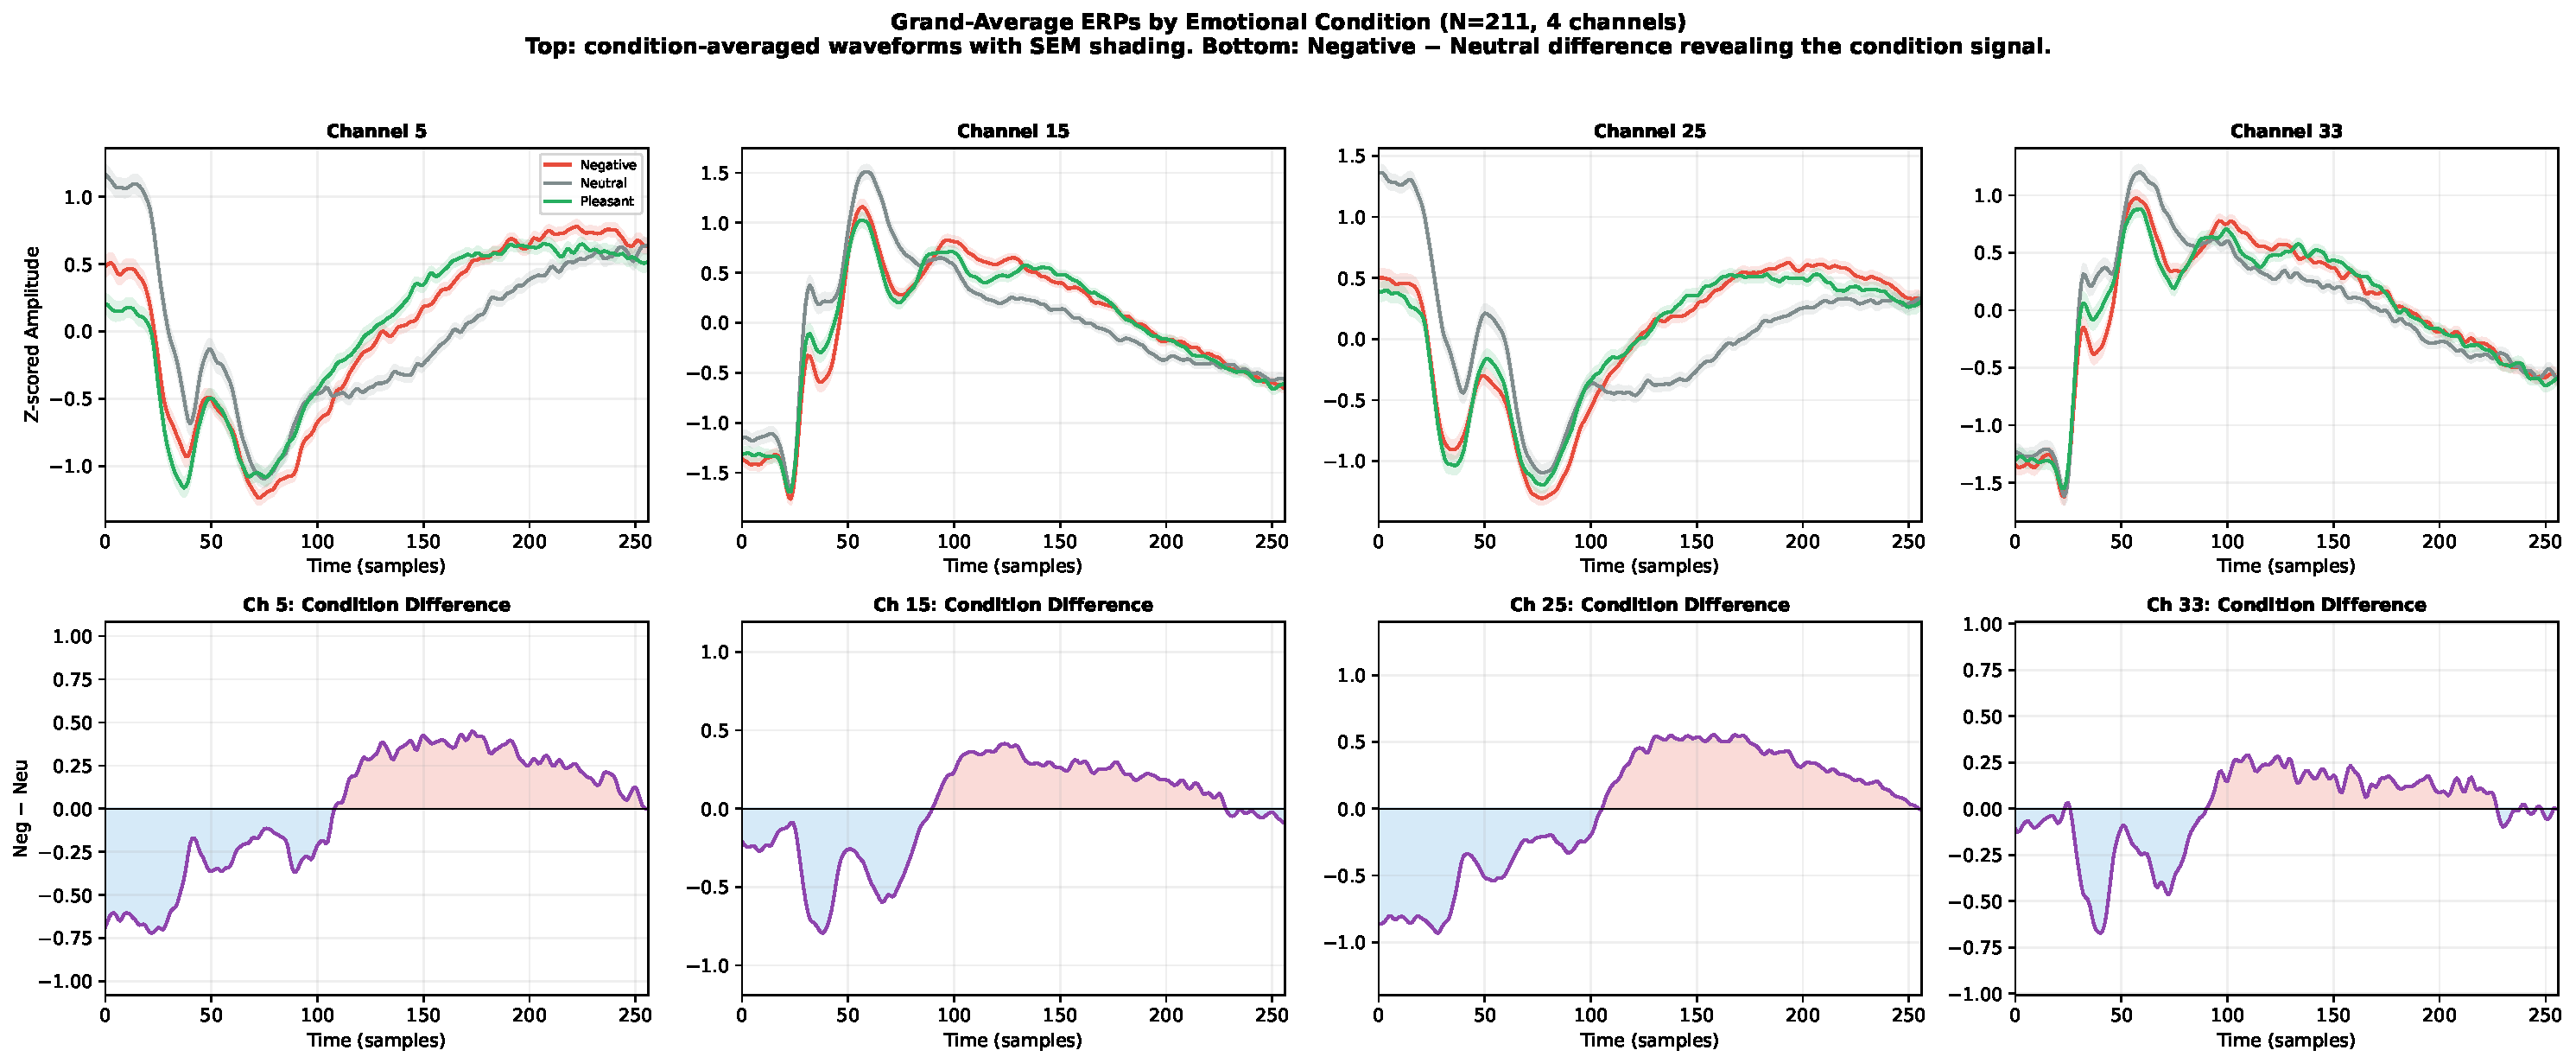
\includegraphics[width=\textwidth]{pictures/chGraphNeuralNetworks/obs08_grand_average_erps.pdf}
    \caption{Grand-average ERPs by condition ($N = 211$). Top: condition-averaged waveforms with SEM shading for four channels. Bottom: Negative $-$ Neutral difference waveforms. Condition effects are small ($5$--$15\%$ of z-scored amplitude) but temporally structured.}
    \label{fig:obs08_erps}
\end{figure}

\subsection{Synthetic-to-Real PCA Transfer Verification}

In the globally fitted per-channel PCA models, $64$ components explain $99.3\%$ of sample variance and the mean component count at $90\%$ variance is seven. Explained variance is not equivalent to retaining class information. Similar eigenvalue spectra also do not make separately fitted component axes comparable across channels. A fold-local common-basis analysis is required for downstream graph construction.

\begin{figure}[H]
    \centering
    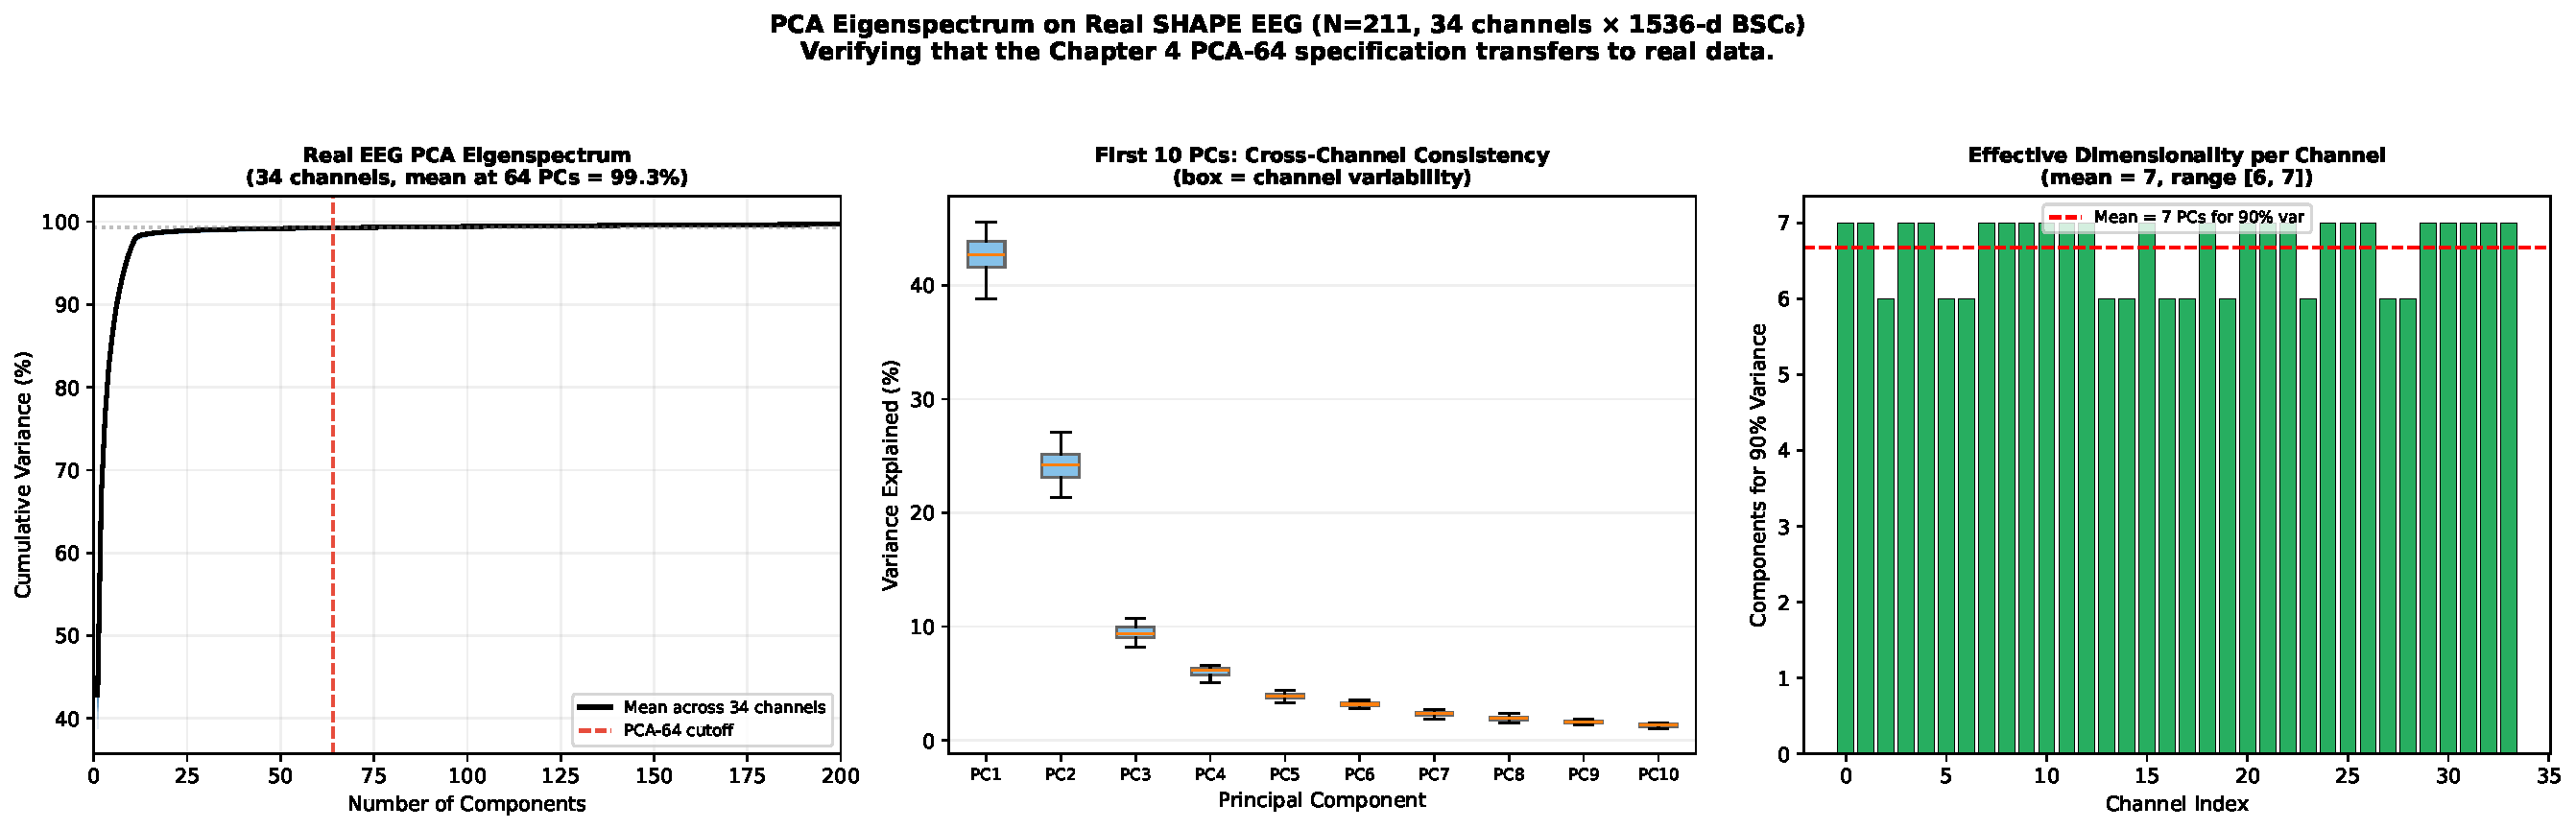
\includegraphics[width=\textwidth]{pictures/chGraphNeuralNetworks/obs09_real_pca_eigenspectrum.pdf}
    \caption{Archived per-channel PCA eigenspectra on SHAPE EEG. Left: cumulative sample-variance curves for all $34$ channels (gray) and their mean (black); 64 components retain $99.3\%$. Center: first ten eigenvalues. Right: six or seven per-channel components reach the $90\%$ sample-variance threshold. Separately fitted axes are not commensurate.}
    \label{fig:obs09_pca}
\end{figure}

\subsection{Feature Space Comparison: Band-Power vs Reservoir}

Figure~\ref{fig:obs10_features} compares the archived feature spaces produced by band-power extraction and reservoir processing. The two-dimensional projections show substantial overlap, and the displayed fold distributions summarize the earlier global-PCA pipeline. Because PCA was fitted before fold separation, the numerical comparison is descriptive and must be recomputed before it can support a performance claim.

\begin{figure}[H]
    \centering
    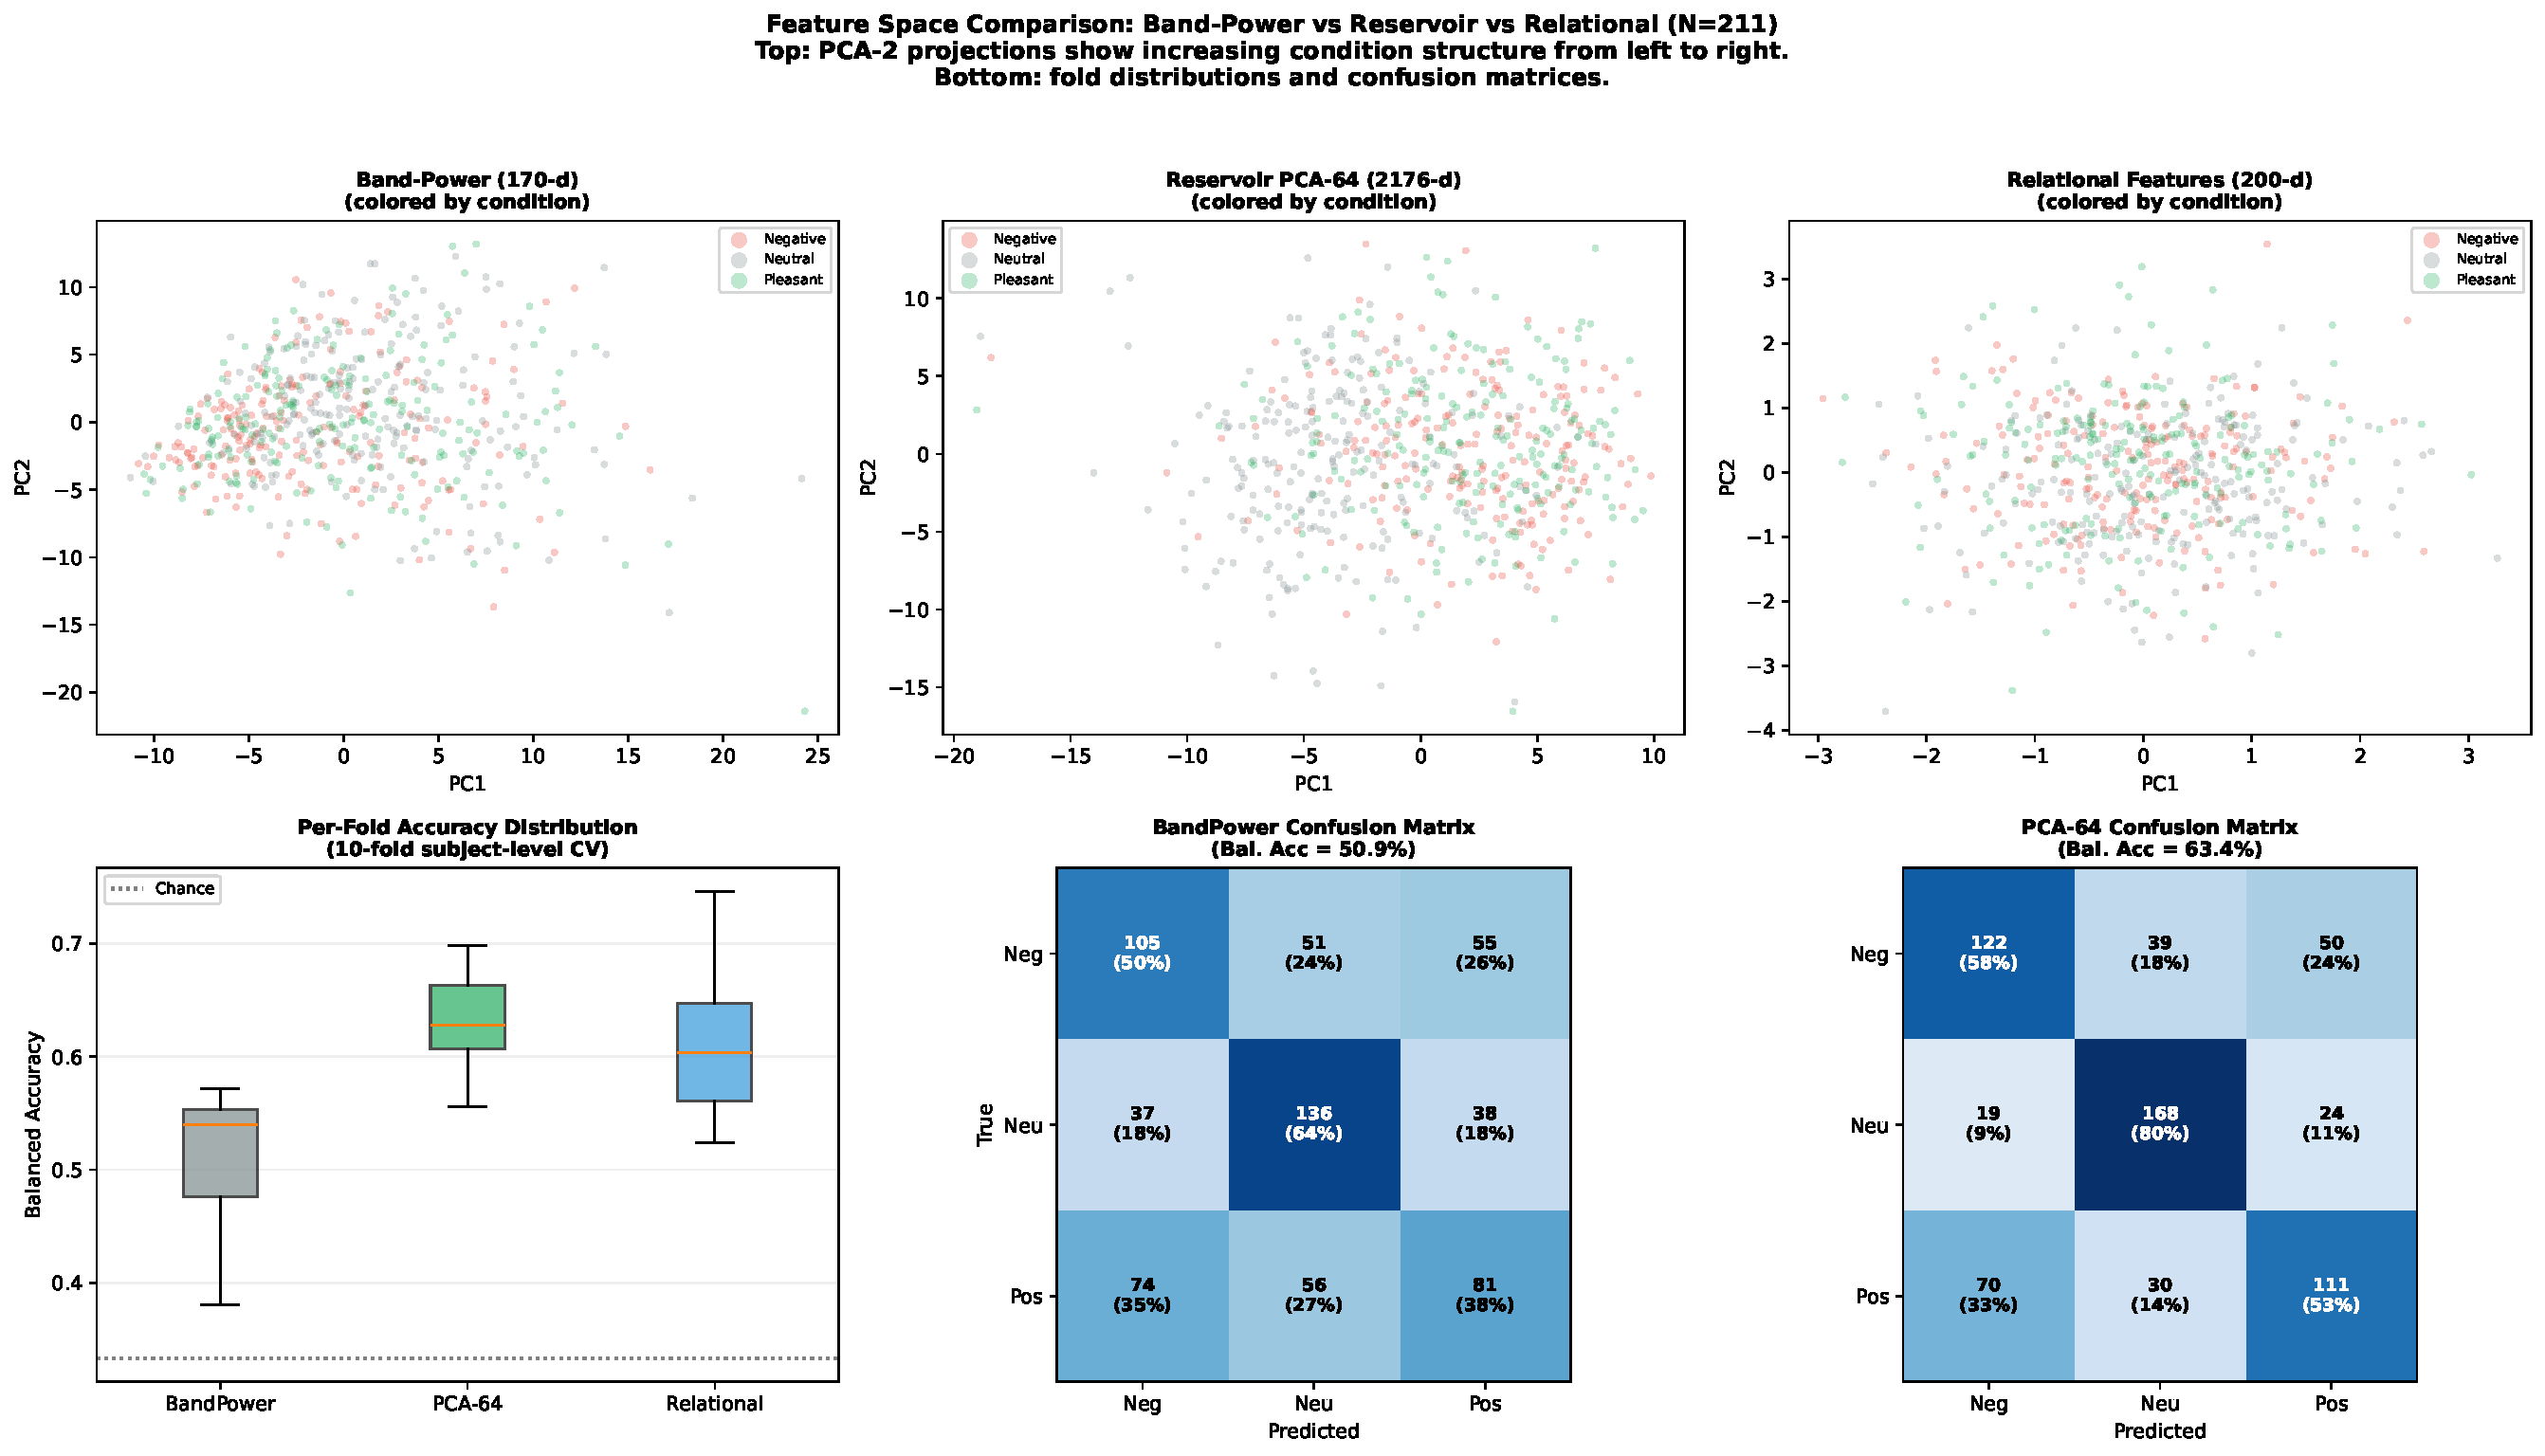
\includegraphics[width=\textwidth]{pictures/chGraphNeuralNetworks/obs10_feature_comparison.pdf}
    \caption{Archived feature-space comparison ($N=211$). The PCA-dependent results use global preprocessing and are descriptive legacy estimates.}
    \label{fig:obs10_features}
\end{figure}

\subsection{Condition-Dependent Graph Topology}

Figure~\ref{fig:obs06_conditions} examines how the archived similarity graphs change across emotional conditions. The three condition-average graphs appear similar at the $20\%$ density threshold, and the edge-difference distribution is centered near zero. The small displayed differences are descriptive; the noncommensurate per-channel PCA axes and lack of multiplicity-adjusted edge inference preclude a claim that a distributed physiological condition signal has been established.

\begin{figure}[H]
    \centering
    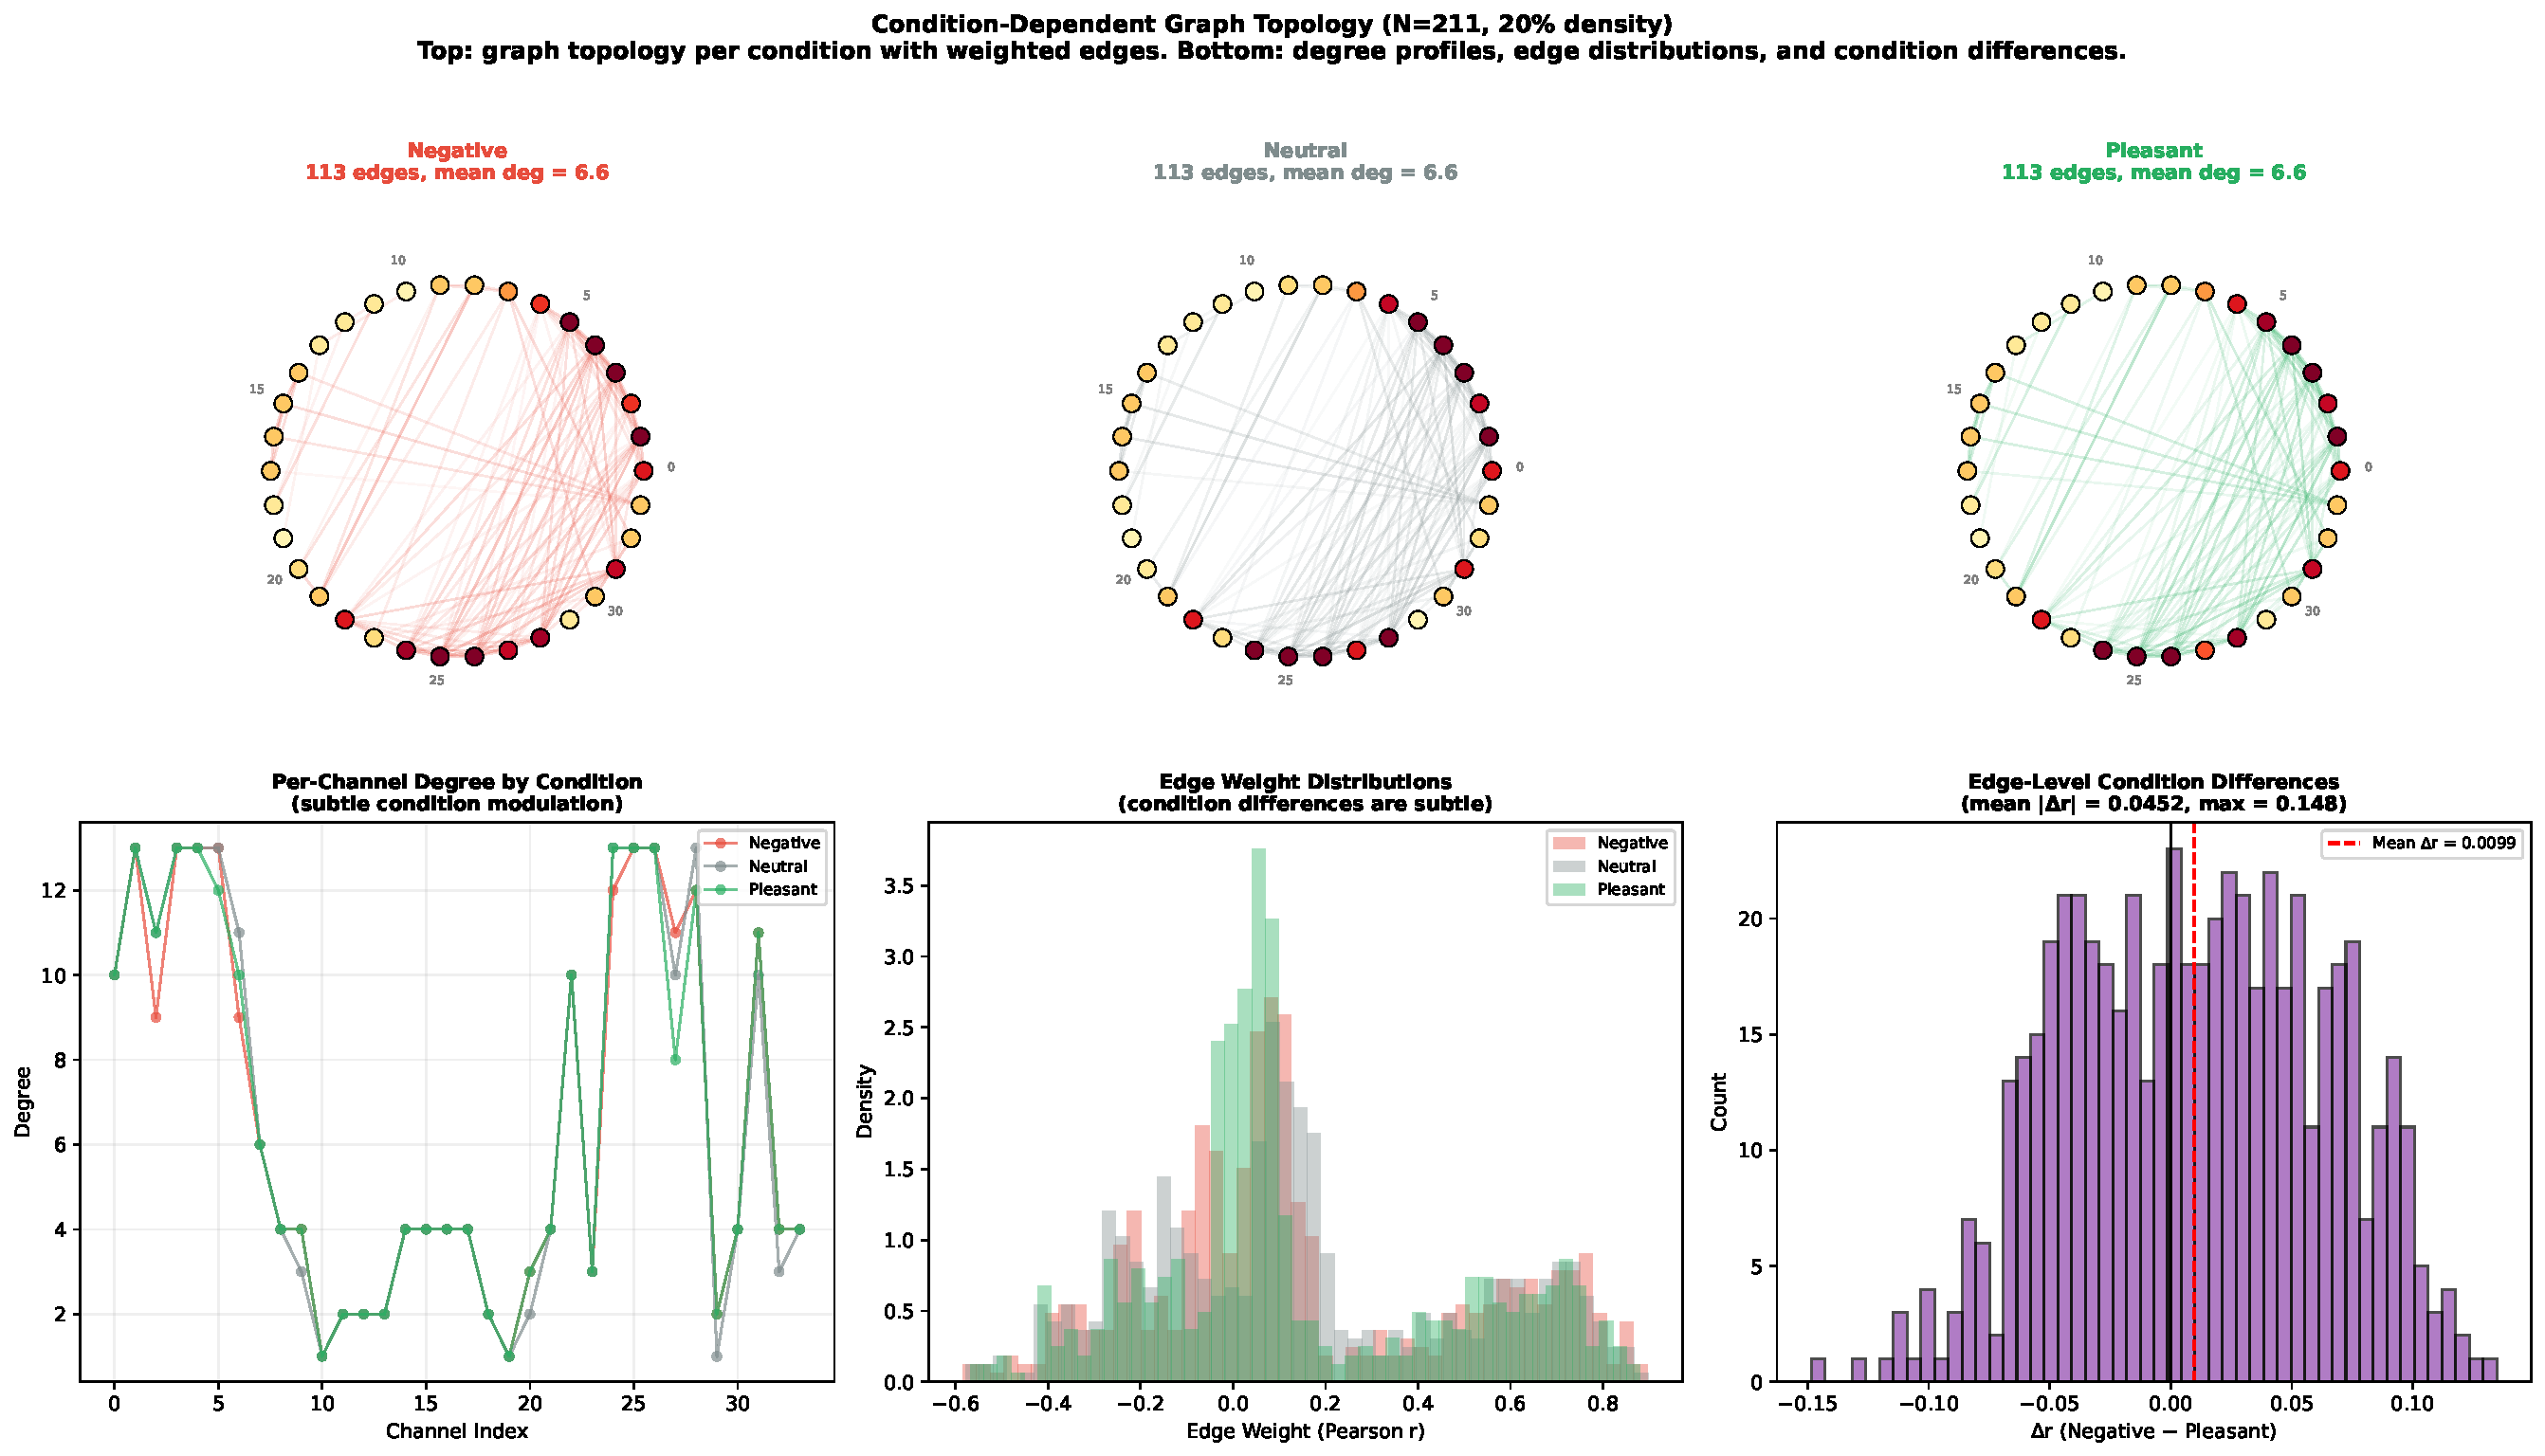
\includegraphics[width=\textwidth]{pictures/chGraphNeuralNetworks/obs06_condition_differences.pdf}
    \caption{Condition-dependent graph topology ($N = 211$). Top: per-condition graphs with weighted edges (node color $=$ degree). Bottom: degree profiles, edge weight distributions, and edge-level condition differences (mean $|\Delta r| = 0.045$).}
    \label{fig:obs06_conditions}
\end{figure}

\subsection{Graph Property Distributions Across Subjects}

Figure~\ref{fig:obs12_properties} summarizes five archived graph properties across the $211$ participants. Mean edge weight has coefficient of variation (CV) $0.22$, mean clustering CV $0.15$, global efficiency CV $0.10$, and degree heterogeneity CV $0.21$. Mean weight and efficiency have Spearman $\rho=0.84$, while degree heterogeneity has $|\rho|<0.15$ with the other displayed metrics. Low rank correlation does not establish statistical independence.

\begin{figure}[H]
    \centering
    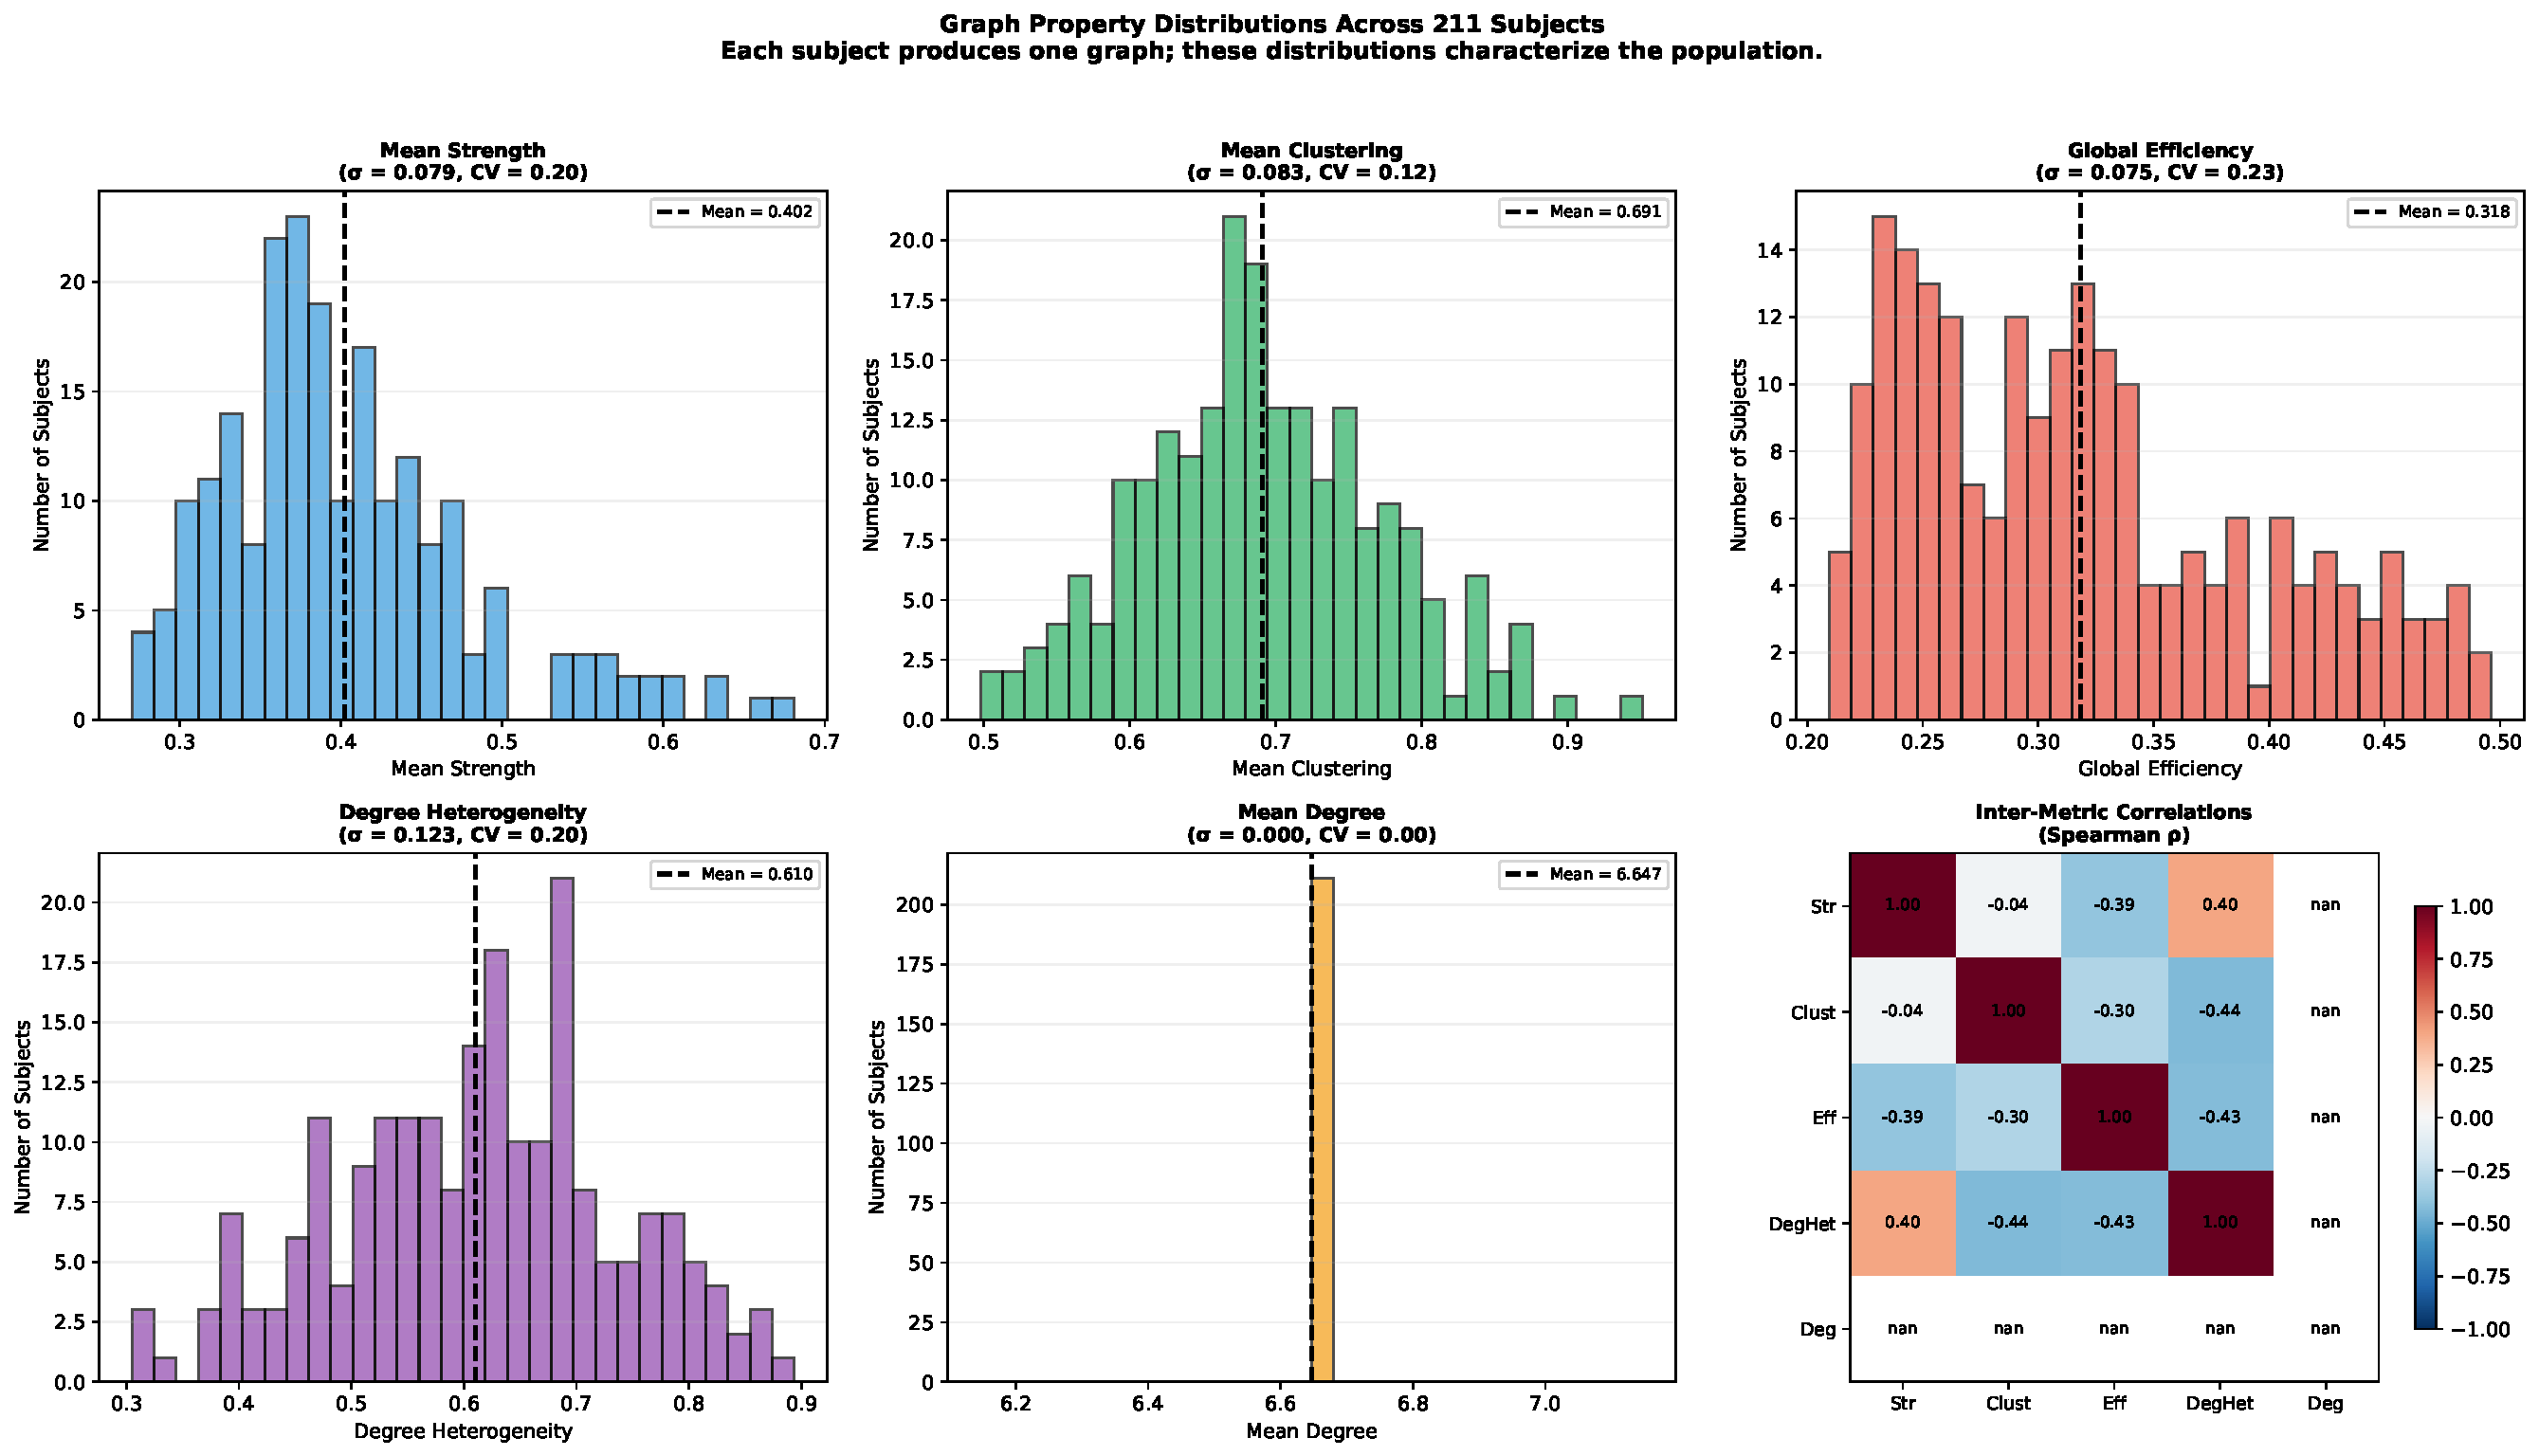
\includegraphics[width=\textwidth]{pictures/chGraphNeuralNetworks/obs12_graph_property_distributions.pdf}
    \caption{Archived graph-property distributions across $211$ participants, with sample means, standard deviations, CVs, and inter-metric Spearman correlations. Mean weight and efficiency have $\rho=0.84$; degree heterogeneity has weak displayed rank correlations with the other metrics.}
    \label{fig:obs12_properties}
\end{figure}

\subsection{Graph Propagation Smoothing Analysis}

Figure~\ref{fig:obs11_variance} illustrates smoothing for one archived graph construction. Inter-channel variance decreases by $33\%$ after two layers and mean cosine similarity increases. These quantities show homogenization, but do not identify how much of the removed variance was discriminative or provide a general criterion for other sensor graphs.

\begin{figure}[H]
    \centering
    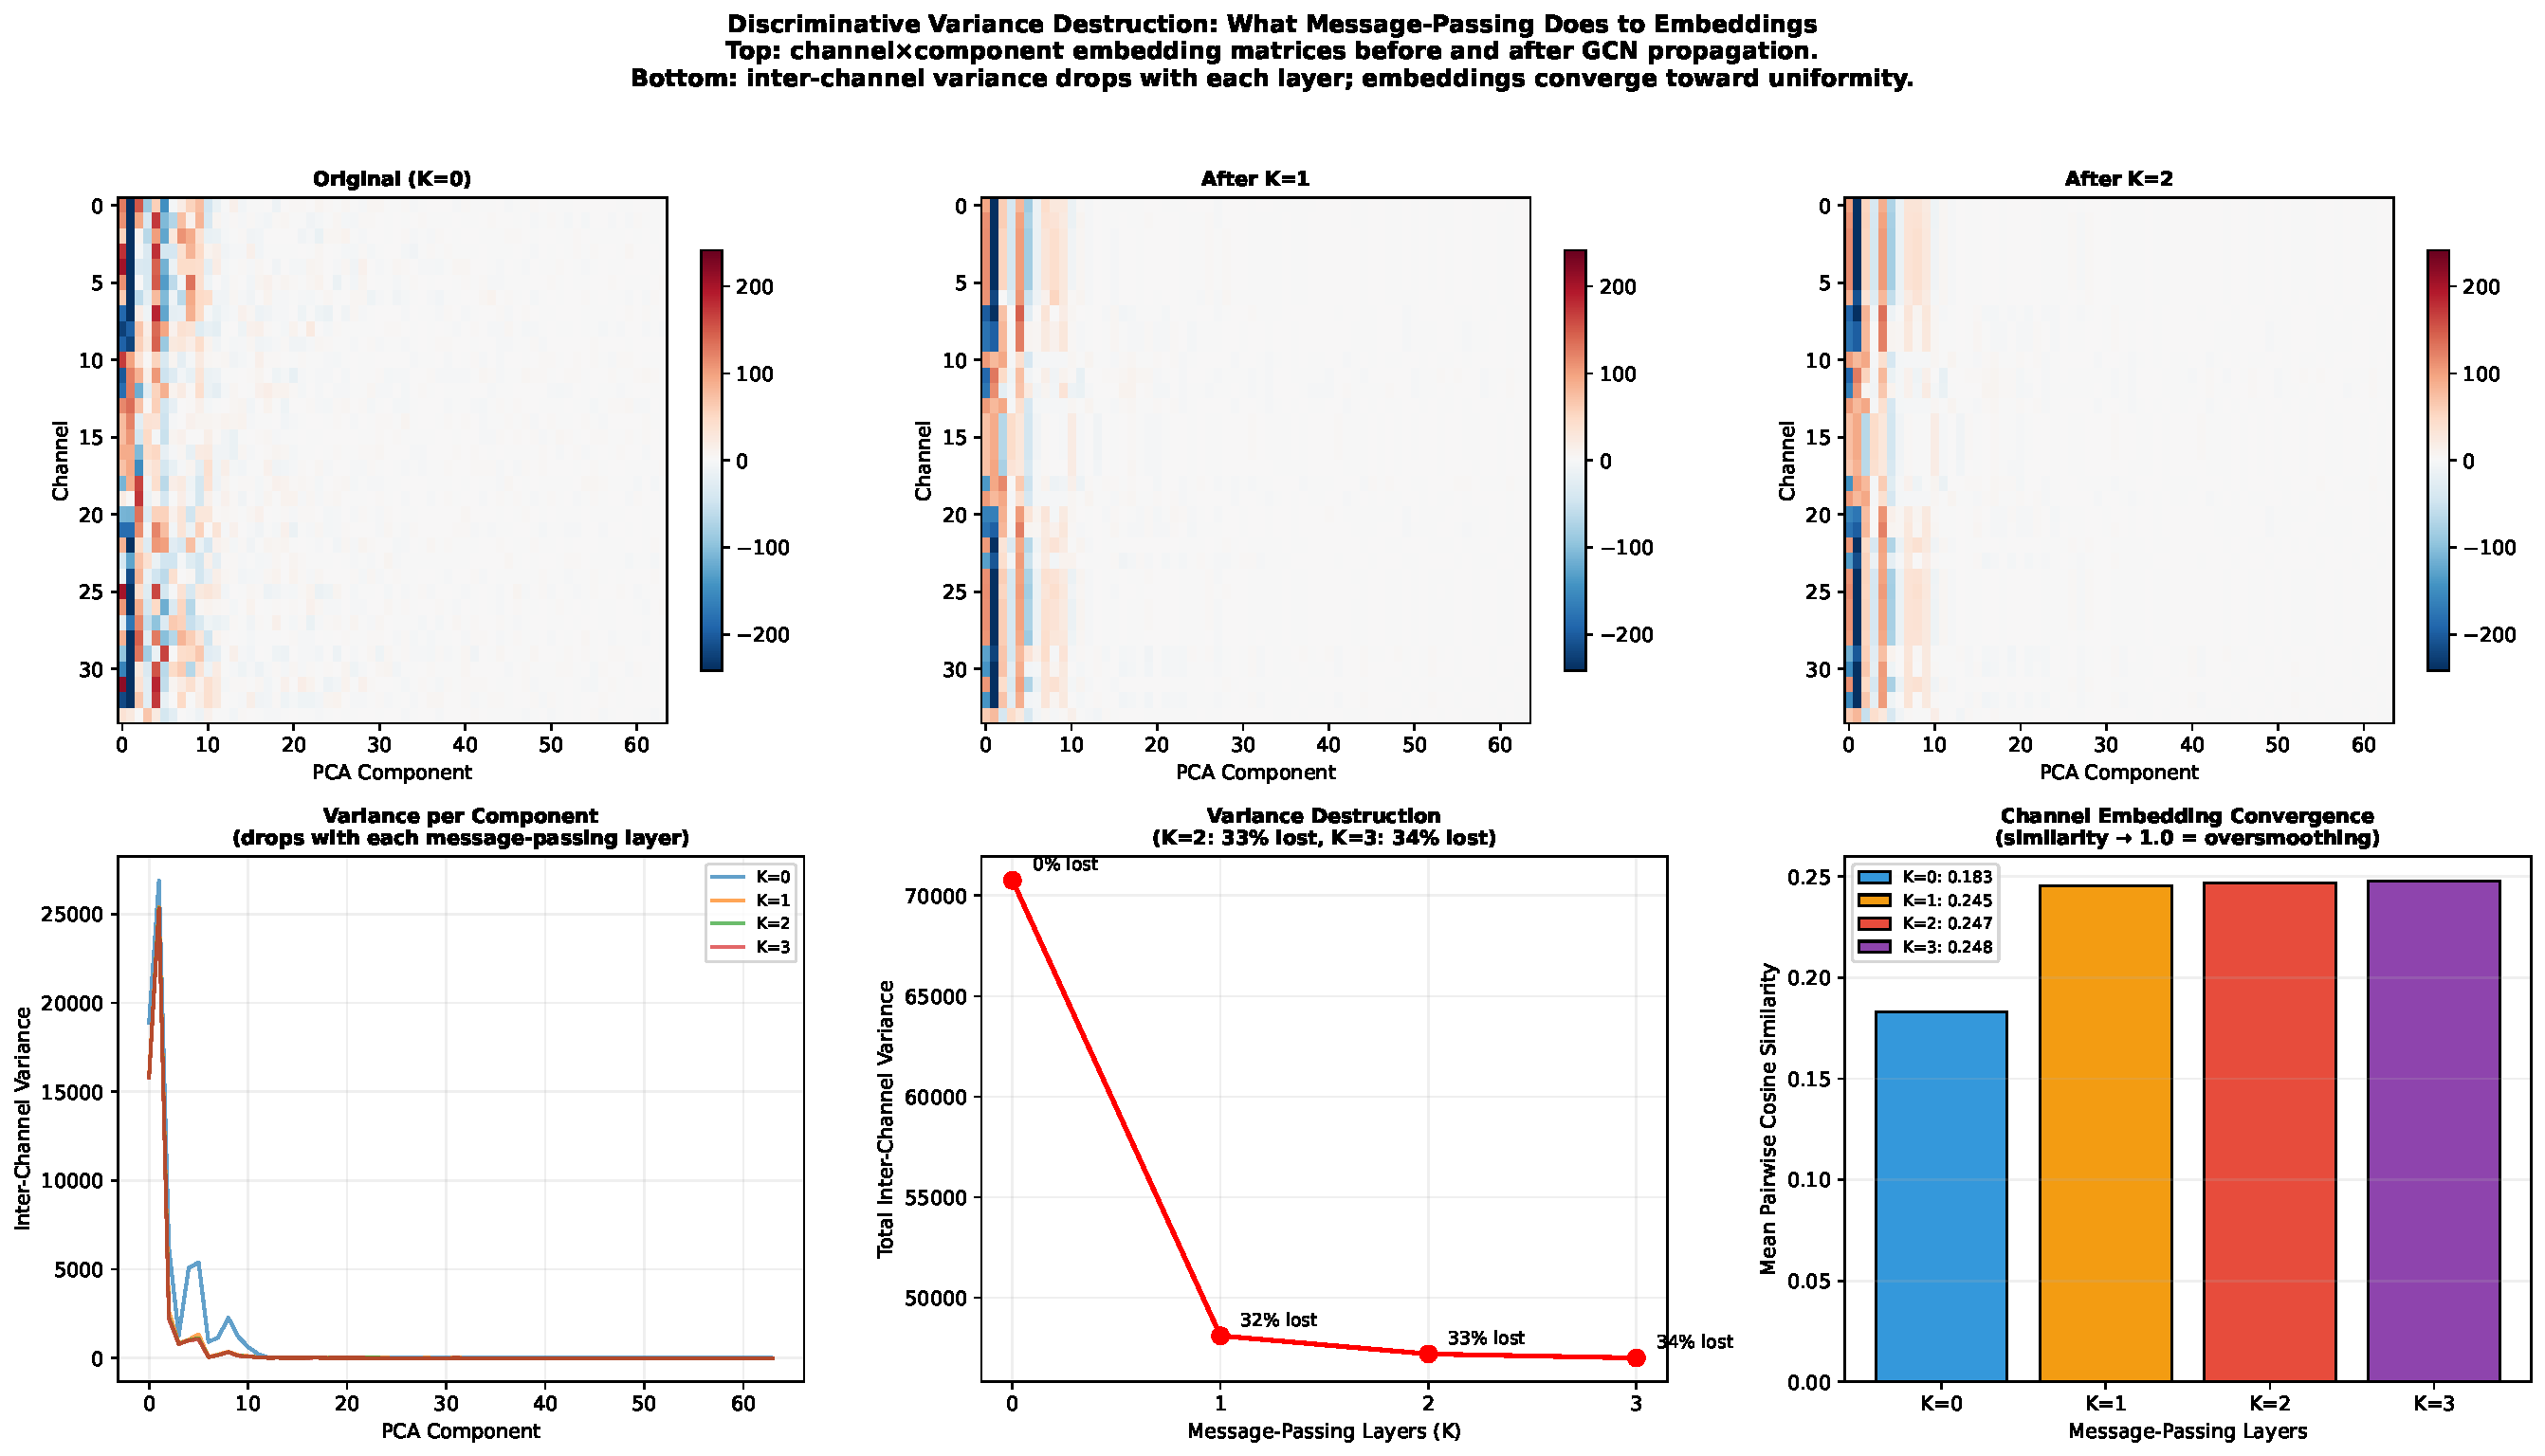
\includegraphics[width=\textwidth]{pictures/chGraphNeuralNetworks/obs11_variance_destruction.pdf}
    \caption{Archived propagation-smoothing illustration. Inter-channel variance decreases and pairwise cosine similarity increases for the displayed construction; no general regime boundary is inferred.}
    \label{fig:obs11_variance}
\end{figure}


\section{Classification Experiments}
\label{sec:ch5_classification}

\subsection{Protocol}

The archived experiments target three-way emotion discrimination ($211$ observations per class) with $10$ subject-grouped folds, so no participant appears in both training and test partitions. However, PCA was fitted before the fold split; subject grouping therefore prevents direct row overlap but does not make PCA-dependent estimates fully held out.

\subsection{Baseline Methods}

Three archived baselines are compared in Table~\ref{tab:baselines}.

\textbf{M1: Band-Power + SVM.} Conventional spectral features ($170$ dimensions) classified by RBF-SVM. No reservoir, no graph.

\textbf{M2: PCA-64 Concatenation + SVM.} The $34 \times 64 = 2{,}176$-dimensional concatenation of all channel embeddings. Uses the reservoir but ignores inter-channel structure.

\textbf{M3: Pairwise Relational Features + SVM.} The $561$ channel-pair embedding differences, PCA-reduced to $200$ dimensions. Graph-informed but without message-passing.

\begin{table}[t]
\centering
\caption{Archived baseline estimates ($N=211$, $633$ observations, 10 subject-grouped folds). PCA-dependent values use global preprocessing and are not unbiased held-out estimates.}
\label{tab:baselines}
\begin{tabular}{llccc}
\hline
\textbf{Method} & \textbf{Features} & \textbf{Dim} & \textbf{Bal.\ Acc.} & \textbf{MCC} \\
\hline
M1: BandPower + SVM & Spectral power & $170$ & $50.9 \pm 6.3\%$ & $0.265$ \\
\textbf{M2: PCA-64 + SVM} & \textbf{Reservoir concat} & $\mathbf{2{,}176}$ & $\mathbf{63.4 \pm 4.4\%}$ & $\mathbf{0.457}$ \\
M3: Relational + SVM & Pairwise diffs & $200$ & $61.8 \pm 7.0\%$ & $0.437$ \\
\hline
\end{tabular}
\end{table}

The displayed M2 estimate is $63.4\%$, $12.5$ percentage points above M1 and $1.6$ points above M3. These are legacy point-estimate differences; global PCA, overlapping nested samples, and the absence of a nested model comparison prevent causal claims about which representation benefits from additional data.

\subsection{Message-Passing GNN Experiments}

Three architectures were evaluated as five-seed ensembles with concatenated graph readouts classified by SVM (Figure~\ref{fig:gnn_comparison}, Table~\ref{tab:gnn_results}). The archived Wilcoxon tests treat ten cross-validation folds as paired observations. Fold scores are dependent because training sets overlap, and PCA was global, so those $p$ values are retained for provenance but not interpreted as confirmatory significance tests.

\begin{figure}[H]
    \centering
    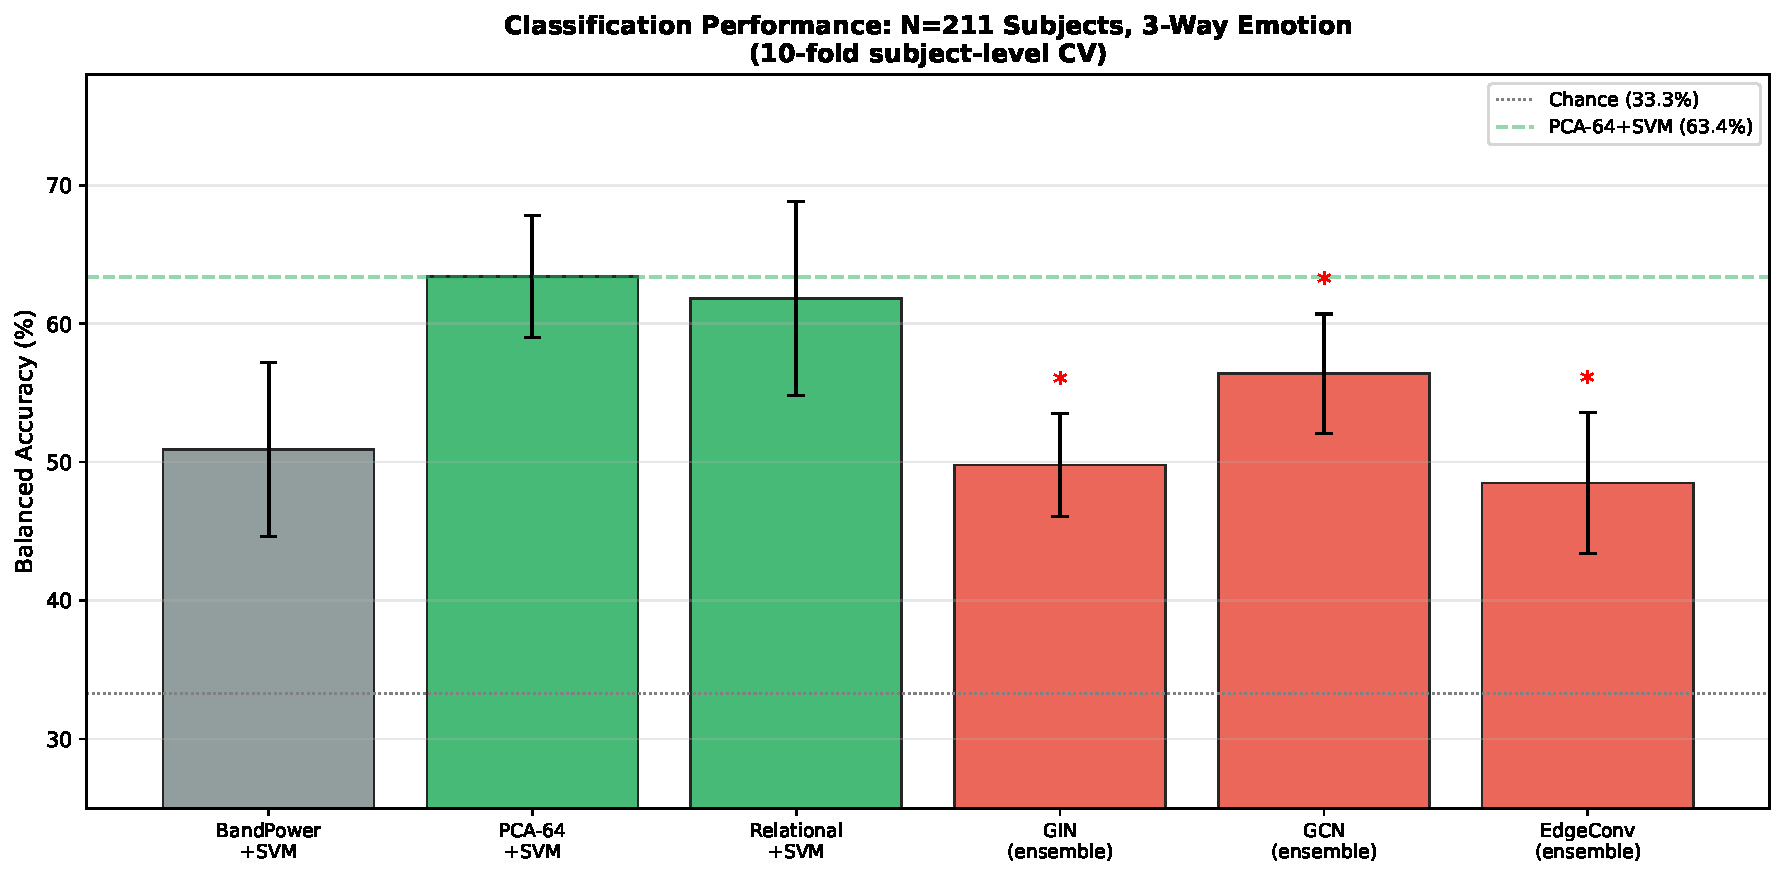
\includegraphics[width=\textwidth]{pictures/chGraphNeuralNetworks/fig_05_gnn_comparison_211.pdf}
    \caption{Archived classification comparison at $N=211$. Asterisks show the original fold-wise tests, which use dependent cross-validation scores and are not interpreted as confirmatory. Chance $=33.3\%$.}
    \label{fig:gnn_comparison}
\end{figure}

\begin{table}[t]
\centering
\caption{Archived message-passing estimates at $N=211$. The displayed $p$ values come from dependent fold-wise comparisons and do not identify a general regime boundary.}
\label{tab:gnn_results}
\begin{tabular}{lcccc}
\hline
\textbf{Architecture} & \textbf{Bal.\ Acc.} & \textbf{MCC} & \textbf{$p$ vs.\ M2} & \textbf{$N\!=\!115$ result} \\
\hline
GIN (5-seed) & $49.8 \pm 3.7\%$ & $0.250$ & $0.004$ & $51.6\%$ \\
GCN (5-seed) & $56.4 \pm 4.3\%$ & $0.349$ & $0.035$ &, \\
EdgeConv (5-seed) & $48.5 \pm 5.1\%$ & $0.234$ & $0.006$ & $53.0\%$ \\
\hline
\end{tabular}
\end{table}

The $N=115$ observations form a subset of the $N=211$ cohort and therefore do not constitute an independent replication. In the archived runs, GIN and EdgeConv did not improve as the larger subset was used, whereas the concatenated baseline did. Differences in training stochasticity, preprocessing, and overlapping samples prevent attributing that pattern to a structural property of EEG graphs. The result is limited to the tested implementations and this cohort.


\subsection{Conventional End-to-End Baselines}

The preceding sections compare ARSPI-Net against spectral features and graph-propagation variants. A natural question is how the reservoir embedding compares against standard trainable models operating directly on the raw multichannel EEG. Table~\ref{tab:conventional_baselines} presents this comparison using the same $10$-fold subject-level cross-validation protocol.

\begin{table}[H]
\centering
\caption{Archived baseline comparison ($N=211$, $633$ observations, 10 subject-grouped folds). Deep models use five-seed ensembles. Centered columns use all three held-out observations per subject and therefore estimate a transductive panel task. PCA-dependent values also use global preprocessing.}
\label{tab:conventional_baselines}
\small
\begin{tabularx}{\textwidth}{@{}>{\raggedright\arraybackslash}Xlcccc@{}}
\hline
\textbf{Method} & \textbf{Input} & \textbf{Dim} & \textbf{Uncent.} & \textbf{Centered} & \textbf{$\Delta$} \\
\hline
\multicolumn{6}{l}{\textit{Spectral features}} \\
BandPower + SVM & Spectral & $170$ & $47.7 \pm 5.1\%$ & $61.0 \pm 6.0\%$ & $+13.3$ \\
\hline
\multicolumn{6}{l}{\textit{Raw EEG, linear readout}} \\
Raw EEG PCA-200 + LogReg & Raw EEG & $200$ & $64.9 \pm 5.0\%$ & $86.4 \pm 4.1\%$ & $+21.5$ \\
Raw EEG (full) + LogReg & Raw EEG & $8{,}704$ & $70.5 \pm 3.0\%$ & $88.4 \pm 2.1\%$ & $+17.9$ \\
\hline
\multicolumn{6}{l}{\textit{Trained deep architectures}} \\
LSTM (bidir, 64h) & Raw EEG & $34 \times 256$ & $58.0 \pm 5.5\%$ & $71.1 \pm 6.8\%$ & $+13.1$ \\
GRU (bidir, 64h) & Raw EEG & $34 \times 256$ & $59.9 \pm 6.4\%$ & $78.4 \pm 3.5\%$ & $+18.5$ \\
\textbf{EEGNet} & \textbf{Raw EEG} & $\mathbf{34 \times 256}$ & $\mathbf{72.0 \pm 4.9\%}$ & $\mathbf{89.1 \pm 3.1\%}$ & $\mathbf{+17.1}$ \\
\hline
\multicolumn{6}{l}{\textit{ARSPI-Net reservoir (fixed recurrent stage)}} \\
Reservoir + LogReg & BSC$_6$/PCA & $2{,}176$ & $59.4 \pm 3.6\%$ & $78.8 \pm 3.4\%$ & $+19.4$ \\
\hline
\end{tabularx}
\end{table}

\begin{figure}[t]
\centering
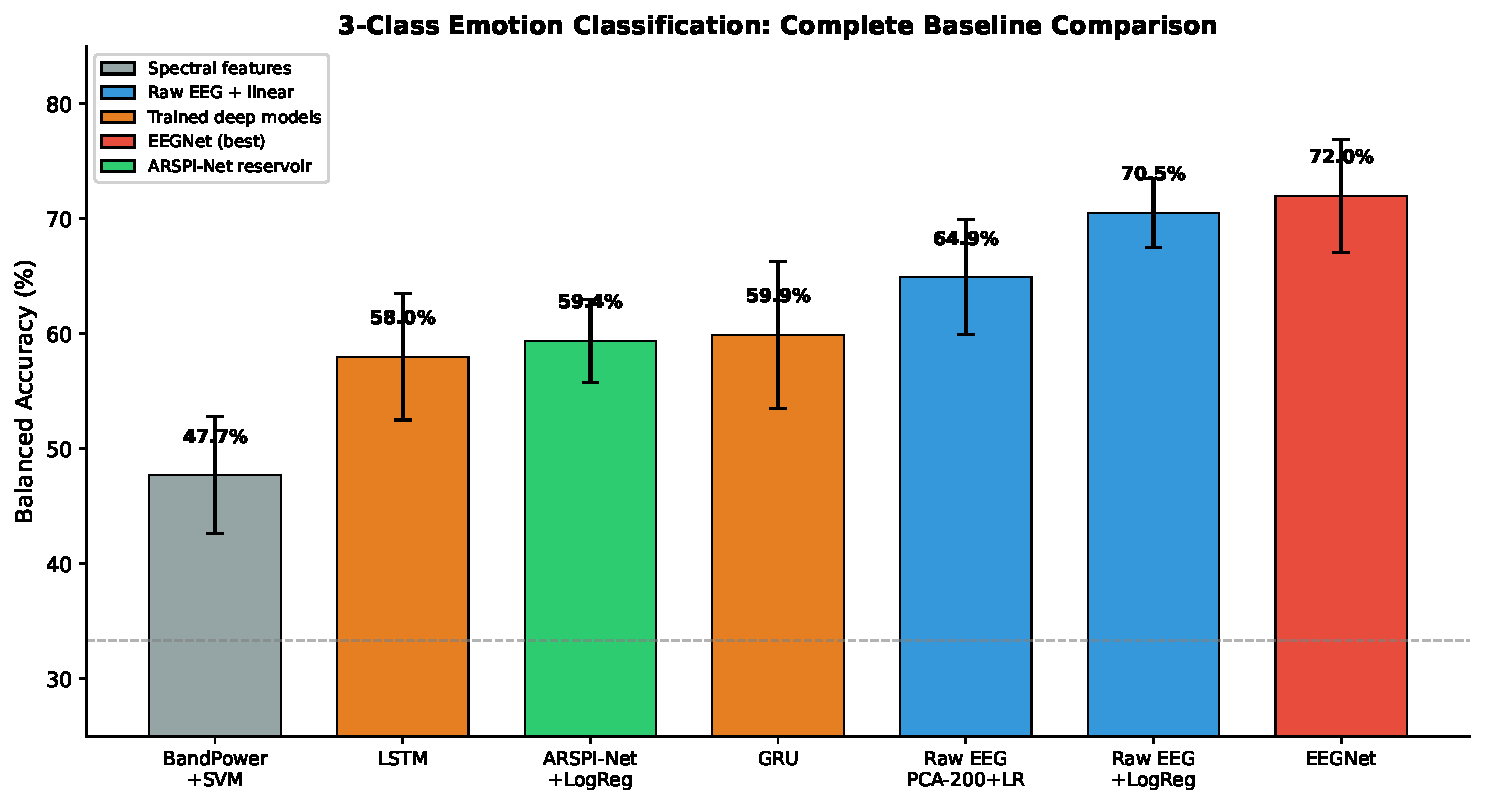
\includegraphics[width=0.85\textwidth]{pictures/chGraphNeuralNetworks/fig_baseline_comparison.pdf}
\caption{Archived baseline comparison on the three-class SHAPE task ($N = 211$, $10$ subject-grouped folds). Right bars use per-subject panel centering. PCA-dependent values were produced by the earlier global-PCA pipeline and are descriptive legacy estimates. Chance $= 33.3\%$.}
\label{fig:baseline_comparison}
\end{figure}

The archived table shows the highest uncentered point estimate for EEGNet ($72.0\%\pm4.9\%$). The reservoir estimate is close to the displayed GRU and LSTM estimates, while the full raw-EEG linear model is higher. The comparison uses different optimization procedures and feature pipelines, so the gaps cannot be attributed to a particular memory--nonlinearity tradeoff.

Panel centering increases every displayed estimate. Because this operation changes the prediction task by using all three held-out observations from each participant, the increase should not be called recovery from underperformance or compared with single-observation deployment. The reservoir exposes specified intermediate variables, but the table does not measure explanation fidelity or compare what alternative models could expose.

\paragraph{Uncertainty and estimand.} The archived fold-wise intervals for centering gains exclude zero for the reported models. Those folds are not independent experimental replications, however, and a post-hoc minimum-detectable-effect calculation does not validate the estimated gains. More importantly, the centered analysis uses a different, transductive estimand because every held-out subject contributes all three condition observations to that subject's normalization. Its values are not directly comparable to single-observation deployment accuracy.

\subsubsection{Interpretation: Inspectable Intermediate Measurements}

The complete baseline table (Table~\ref{tab:conventional_baselines}) distinguishes predictive performance from representation analysis. EEGNet achieves the highest centered accuracy ($89.1\%$), while raw EEG with a linear readout reaches $88.4\%$. Neither baseline is evaluated with the same predefined dynamical and topological descriptors used for ARSPI-Net, so the comparison concerns the analyses performed here rather than the inherent interpretability of every possible implementation.

The pipeline produces a classification output and specified intermediate summaries. Fixed recurrent weights make the transformation repeatable for a saved initialization and parameter set. The spike count has a defined computational unit; PCA coordinates and graph summaries are dimensionless model quantities. Explicit construction improves traceability but does not supply clinical meaning.

The roughly ten-point difference between the displayed centered raw-EEG and reservoir estimates cannot be converted into an information-theoretic quantity. It may reflect compression, model capacity, optimization, preprocessing, or sampling. The reservoir was analyzed with a predefined set of intermediate summaries; the comparison did not test whether analogous summaries or attribution methods could be constructed for the raw-EEG model.


\section{Representation Geometry: Variance Decomposition and Signal Detection}
\label{sec:ch5_variance}

The classification results raise a question motivated by signal detection theory: what is the structure of the representation space in which the classifier operates, and what are the dominant sources of variance?

\subsection{Variance Decomposition}

An archived one-way decomposition of the $2{,}176$-dimensional concatenated embedding assigns a larger sample sum-of-squares fraction to participant than to condition (Figure~\ref{fig:exp01_variance}). Because the transformation was fitted globally, the result is a property of that in-sample representation rather than a population estimate of latent subject identity.

\begin{figure}[H]
    \centering
    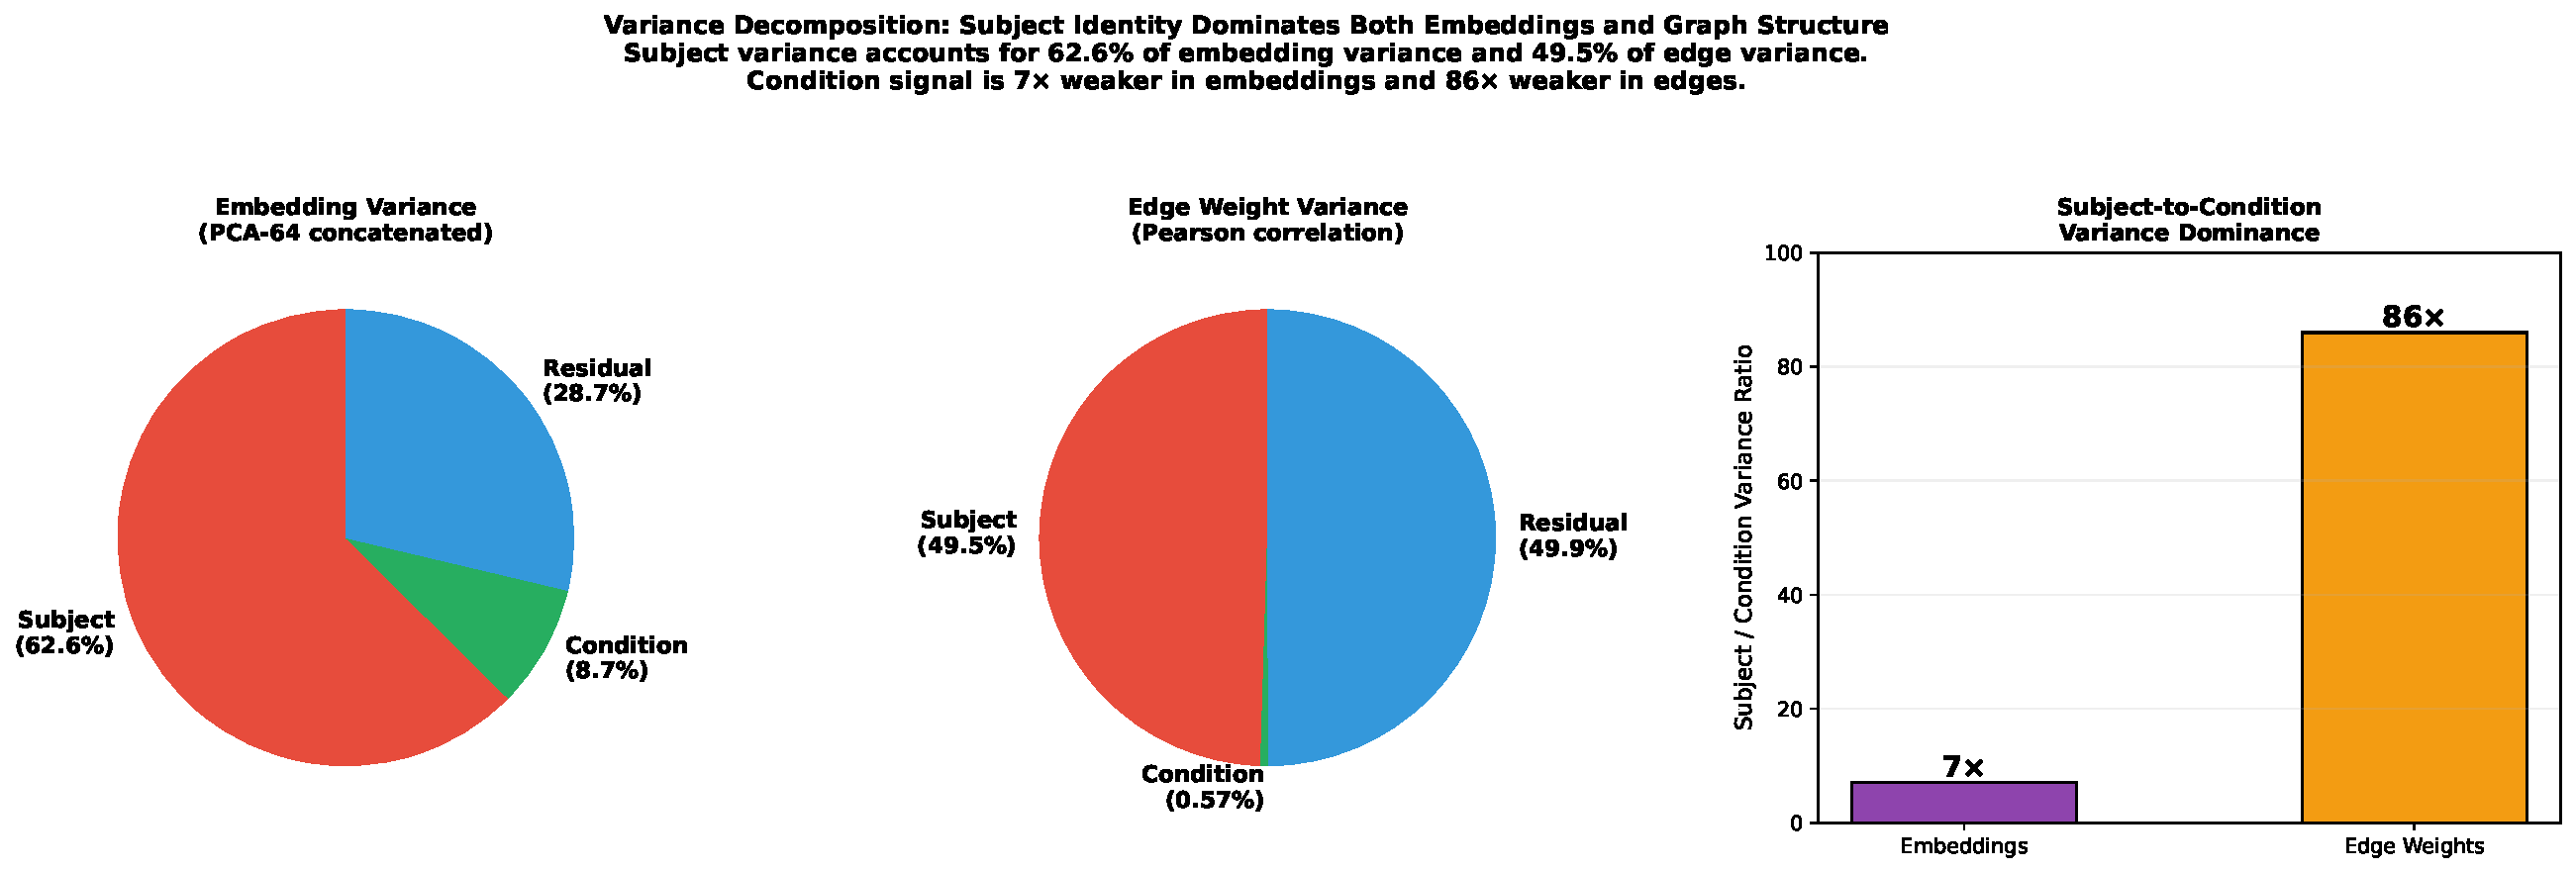
\includegraphics[width=\textwidth]{pictures/chGraphNeuralNetworks/exp01_variance_decomposition.pdf}
    \caption{Descriptive variance decomposition of the archived embedding and edge-weight spaces. Left: embedding partition (subject $62.6\%$, condition $8.7\%$, residual $28.7\%$). Center: edge-weight partition (subject $49.5\%$, condition $0.57\%$). Right: subject-to-condition ratios. These values depend on the earlier global-PCA graph construction.}
    \label{fig:exp01_variance}
\end{figure}

Subject identity accounts for $62.6\%$ of total embedding variance, emotional condition accounts for $8.7\%$, and within-subject residual variability accounts for $28.7\%$, a $7\times$ subject-to-condition ratio. At the graph-edge level, the dominance is more extreme: subject identity accounts for $49.5\%$ of edge-weight variance, condition accounts for only $0.57\%$ ($86\times$ ratio), and residual accounts for $49.9\%$. The classifier must detect an $8.7\%$ condition signal embedded in a representation dominated by subject-identity structure.

\subsection{Subject-Nuisance Suppression: Revealing the True Condition Signal}

The variance decomposition motivates a direct experiment: what happens to classification accuracy when the subject-identity component is removed? Six nuisance-suppression strategies were evaluated (Figure~\ref{fig:exp07_nuisance}).

\begin{figure}[H]
    \centering
    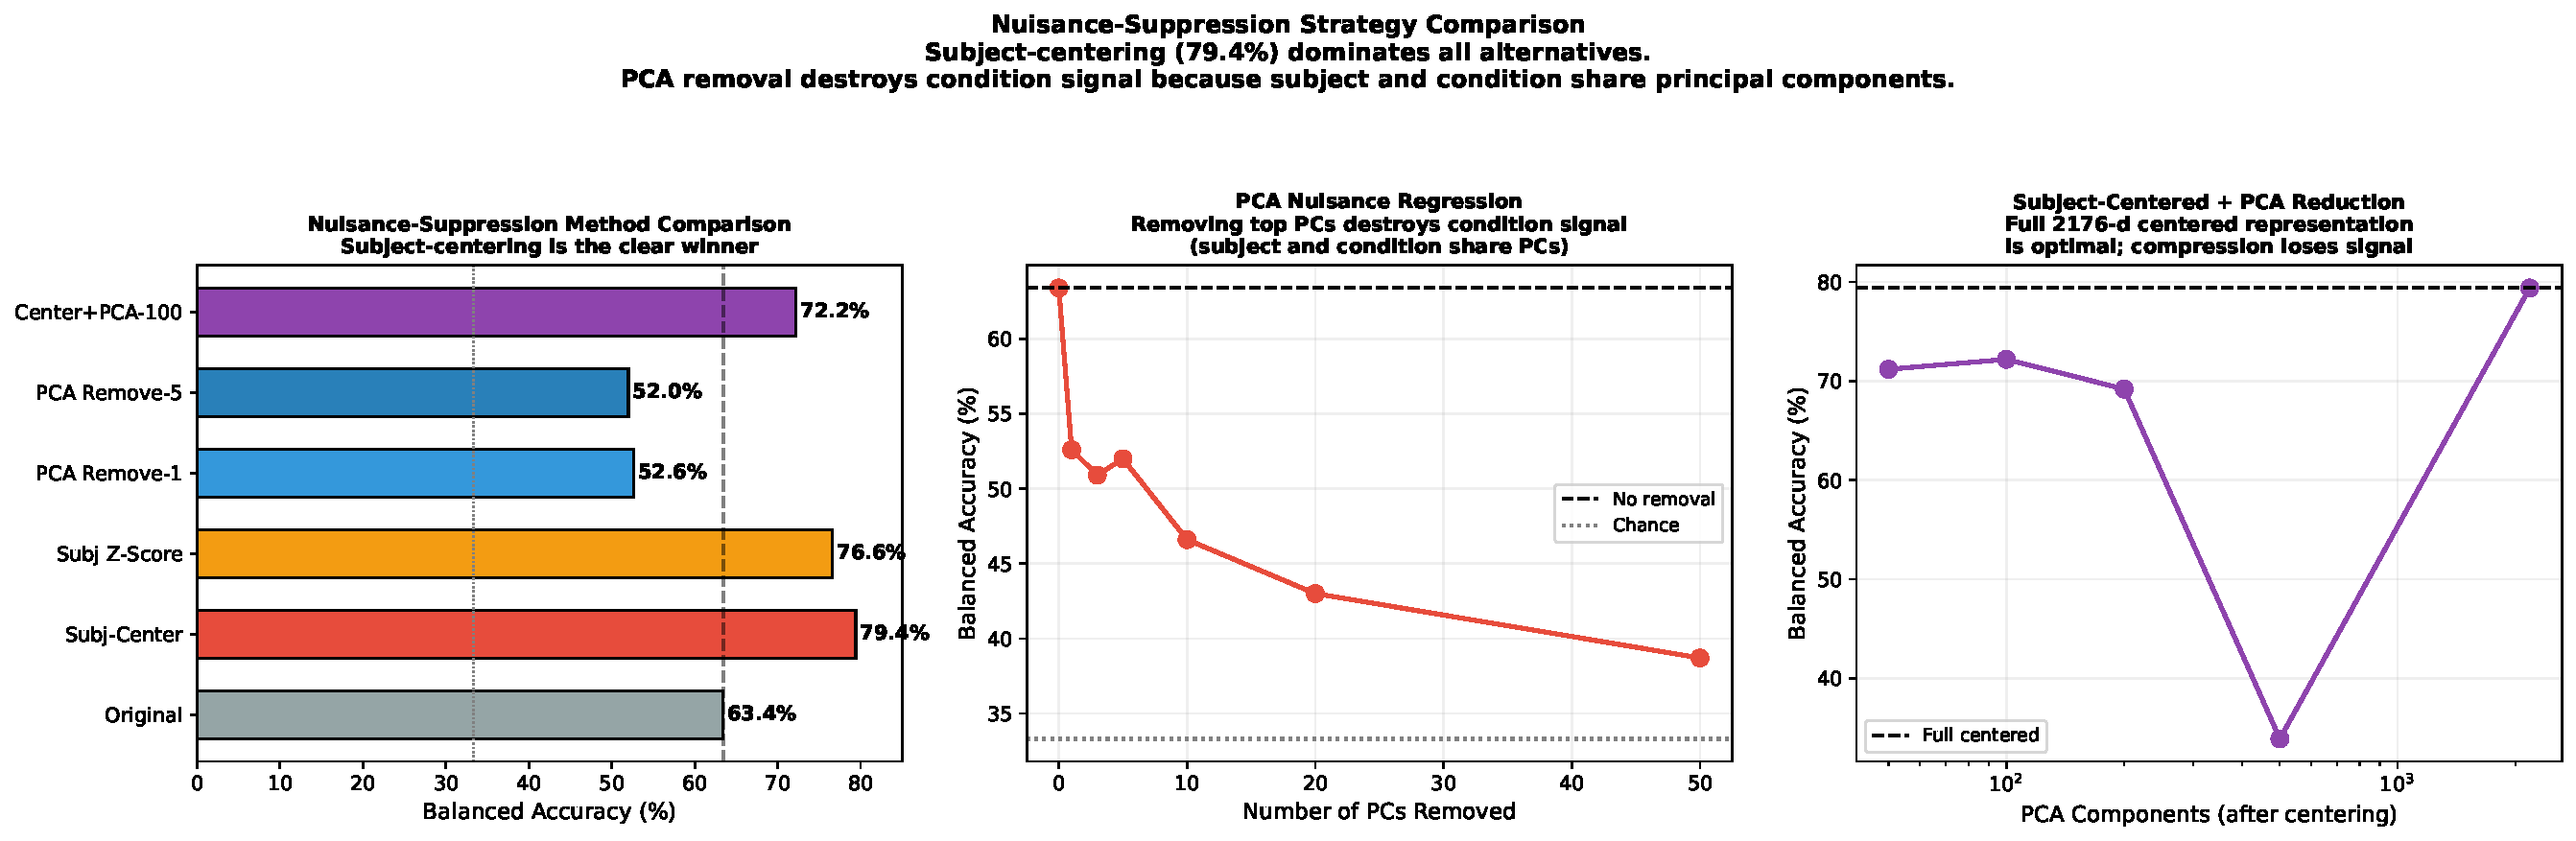
\includegraphics[width=\textwidth]{pictures/chGraphNeuralNetworks/exp07_nuisance_comparison.pdf}
    \caption{Archived normalization comparison. Per-subject centering uses all three observations from each held-out subject and is therefore a transductive panel analysis, not a single-observation deployment estimate. PCA-dependent values also use the earlier global-PCA representation.}
    \label{fig:exp07_nuisance}
\end{figure}

In the archived analysis, per-subject centering---subtracting each subject's mean embedding across all three conditions---produces $79.4\% \pm 7.4\%$ balanced accuracy, compared with $63.4\%$ without centering. Within-subject z-scoring produces $76.6\% \pm 5.9\%$. These values describe a repeated-measures panel setting in which all three observations for a held-out subject are available together; they do not estimate performance for a new subject represented by a single observation.

PCA nuisance regression (projecting out the top-$k$ components) reduces the archived accuracy as more components are removed. This is consistent with, but does not prove, overlap between directions associated with subject and condition variation. Because PCA was fitted globally and the directions are data-dependent, the experiment cannot establish a population-level geometric identity between the two sources of variation.

Subject-centering followed by PCA compression to $100$ dimensions produces $72.2\%$ in the archived run, below the full $2{,}176$-dimensional centered value. That difference may reflect information loss, regularization, or preprocessing choices; it does not by itself locate condition information across dimensions.

\subsubsection{Methodological Status of Subject-Centering}

The operational definition of per-subject centering is: given all $K$ observations from subject $s$ (here $K = 3$, one per condition), compute the subject mean $\bar{\mathbf{x}}_s = \frac{1}{K}\sum_{k=1}^K \mathbf{x}_{s,k}$ and subtract it from each observation: $\tilde{\mathbf{x}}_{s,k} = \mathbf{x}_{s,k} - \bar{\mathbf{x}}_s$. This is equivalent to the within-subject deviation from the subject's own baseline, the standard operation in repeated-measures experimental design.

Two methodological points require explicit statement. First, subject-centering uses all three held-out observations from each test subject. No labels and no training-subject observations enter that calculation, and no subject appears in both training and test folds. Nevertheless, the procedure uses feature data from the entire test-subject panel, so it is transductive with respect to the held-out subject and should be described as panel normalization rather than ordinary prospective prediction.

Second, per-subject centering is unavailable when a prospective subject contributes only one condition. The $79.4\%$ value is therefore neither a deployment estimate nor a theoretical ceiling; it is a descriptive result for the three-observation panel estimand. A prospective alternative would need to be specified, trained without access to held-out panels, and evaluated independently.

\subsection{Detection-Theoretic Analysis}

The archived analysis also summarized Negative--Neutral class geometry. Let $\mathbf{x} \in \mathbb{R}^d$ denote a representation vector with class-conditional means $\boldsymbol{\mu}_c$ and covariances $\boldsymbol{\Sigma}_c$. Four retained summaries describe different aspects of separation; none is an independent estimate of generalization performance.

\textbf{Sensitivity index (d$'$)} measures the standardized mean difference along each feature dimension: $d'_j = |\mu_{0,j} - \mu_{1,j}| / \sqrt{(\sigma_{0,j}^2 + \sigma_{1,j}^2)/2}$. The mean and maximum over dimensions characterize the average and peak per-feature discriminability.

\textbf{Bhattacharyya distance} summarizes overlap under a Gaussian approximation and can be used in bounds on Bayes error. Here it is computed with diagonal covariance matrices:
\begin{equation}
D_B = \frac{1}{8}(\boldsymbol{\mu}_0-\boldsymbol{\mu}_1)^\top
\boldsymbol{\Sigma}_{\mathrm{avg}}^{-1}(\boldsymbol{\mu}_0-\boldsymbol{\mu}_1)
+\frac{1}{2}\ln\!\left(
\frac{|\boldsymbol{\Sigma}_{\mathrm{avg}}|}
{|\boldsymbol{\Sigma}_0|^{1/2}|\boldsymbol{\Sigma}_1|^{1/2}}
\right).
\end{equation}

\textbf{Fisher Discriminant Ratio} measures the ratio of between-class to within-class scatter: FDR $= \text{tr}(\mathbf{S}_W^{-1}\mathbf{S}_B)$, with Tikhonov regularization for rank-deficient $\mathbf{S}_W$.

\textbf{Mahalanobis distance} is $d_M = \sqrt{(\boldsymbol{\mu}_0 - \boldsymbol{\mu}_1)^\top \boldsymbol{\Sigma}_{\text{pool}}^{-1} (\boldsymbol{\mu}_0 - \boldsymbol{\mu}_1)}$, measuring class separation in pooled-covariance-normalized space.

An earlier version also reported $\tfrac{1}{2}\sum_j\ln(1+d_j'^2)$ as a mutual-information lower bound. That expression is not a valid general lower bound for these correlated, multiclass features and can exceed the entropy of the three-class label. It is therefore omitted from the interpretation.

\begin{figure}[H]
    \centering
    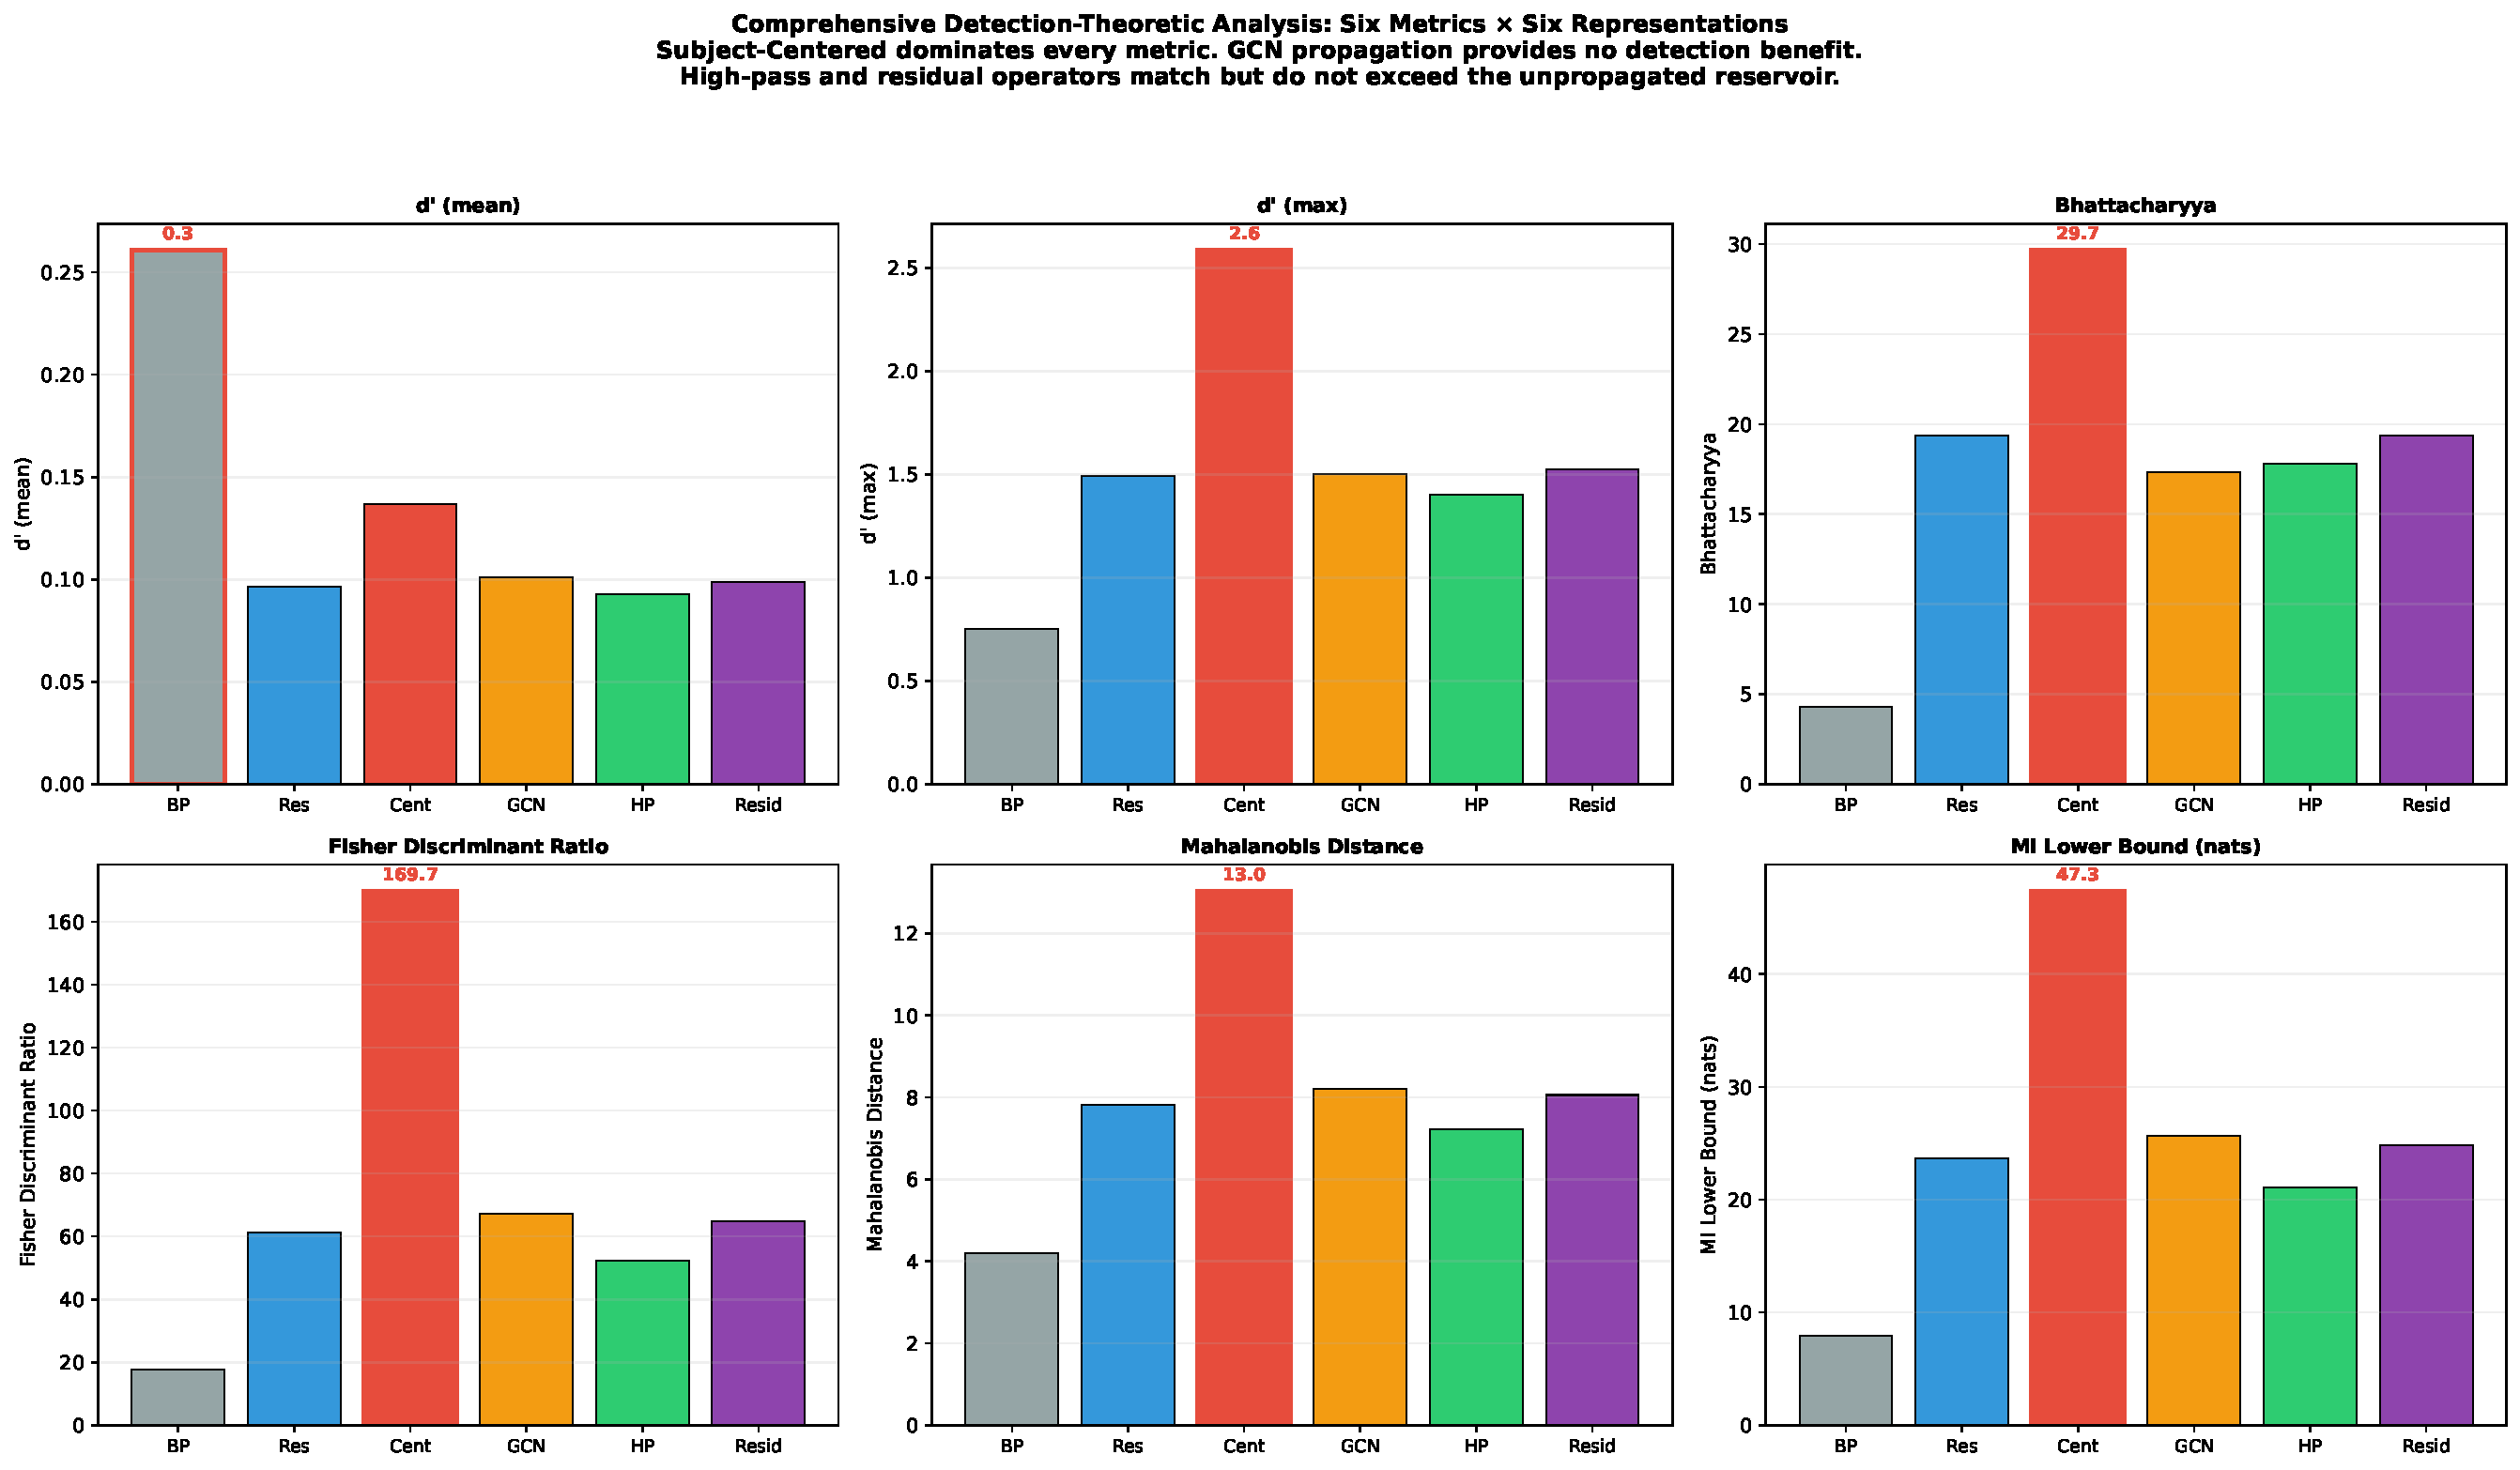
\includegraphics[width=\textwidth]{pictures/chGraphNeuralNetworks/exp08_detection_metrics.pdf}
    \caption{Archived class-geometry summaries for Negative versus Neutral. The mutual-information panel in the archived figure used an invalid estimator and is not interpreted. PCA-dependent quantities are descriptive because the earlier pipeline fitted PCA globally.}
    \label{fig:exp08_detection}
\end{figure}

In the archived representation, the reservoir features have maximum sensitivity index $d'_{\max}=1.49$, diagonal-approximation Bhattacharyya distance $19.4$, Fisher ratio $61.1$, and regularized Mahalanobis distance $7.82$. The corresponding panel-centered values are larger. These in-sample summaries depend on global preprocessing and covariance regularization, so they are descriptive comparisons rather than a count of information units.

\subsubsection{Spectral Interpretation of the Archived Propagation Sweep}

Let $\hat{\mathbf{A}}$ denote a symmetric normalized adjacency with eigendecomposition $\hat{\mathbf{A}}=\mathbf{U}\boldsymbol{\Lambda}\mathbf{U}^{\top}$. Linear propagation gives $\mathbf{H}^{(K)}=\hat{\mathbf{A}}^K\mathbf{H}^{(0)}=\mathbf{U}\boldsymbol{\Lambda}^K\mathbf{U}^{\top}\mathbf{H}^{(0)}$. Thus a graph-spectral component associated with eigenvalue $\mu_i$ is multiplied by $\mu_i^K$.

This identity explains spectral attenuation, but attenuation alone does not prove that standardized class detectability must decrease: propagation can change class means and within-class covariance together. The archived sweep shows decreasing accuracy for the tested operators and graphs, which is consistent with useful contrast being attenuated in those runs. It does not establish a general propagation--detectability theorem.

Per-subject centering operates across a subject's observations, whereas graph propagation operates across channel nodes. The subject mean is therefore not the channel graph's zero-frequency component, and the two operations should not be assigned complementary graph-frequency roles. Their empirical effects are reported separately.


\section{Graph Propagation Regime Characterization}
\label{sec:ch5_regime}

In the archived implementation, message-passing propagation does not improve the displayed classification result. The propagation sweep describes how that implementation changes as depth and density vary; it does not locate a universal regime boundary.

\subsection{Propagation Operating Characteristic}

Figure~\ref{fig:exp03_poc} presents accuracy, inter-channel variance, and pairwise cosine similarity across propagation depths from $0$ to $5$. Graph densities are $5\%$, $10\%$, $15\%$, $20\%$, $30\%$, and $50\%$, producing $36$ operating points.

\begin{figure}[H]
    \centering
    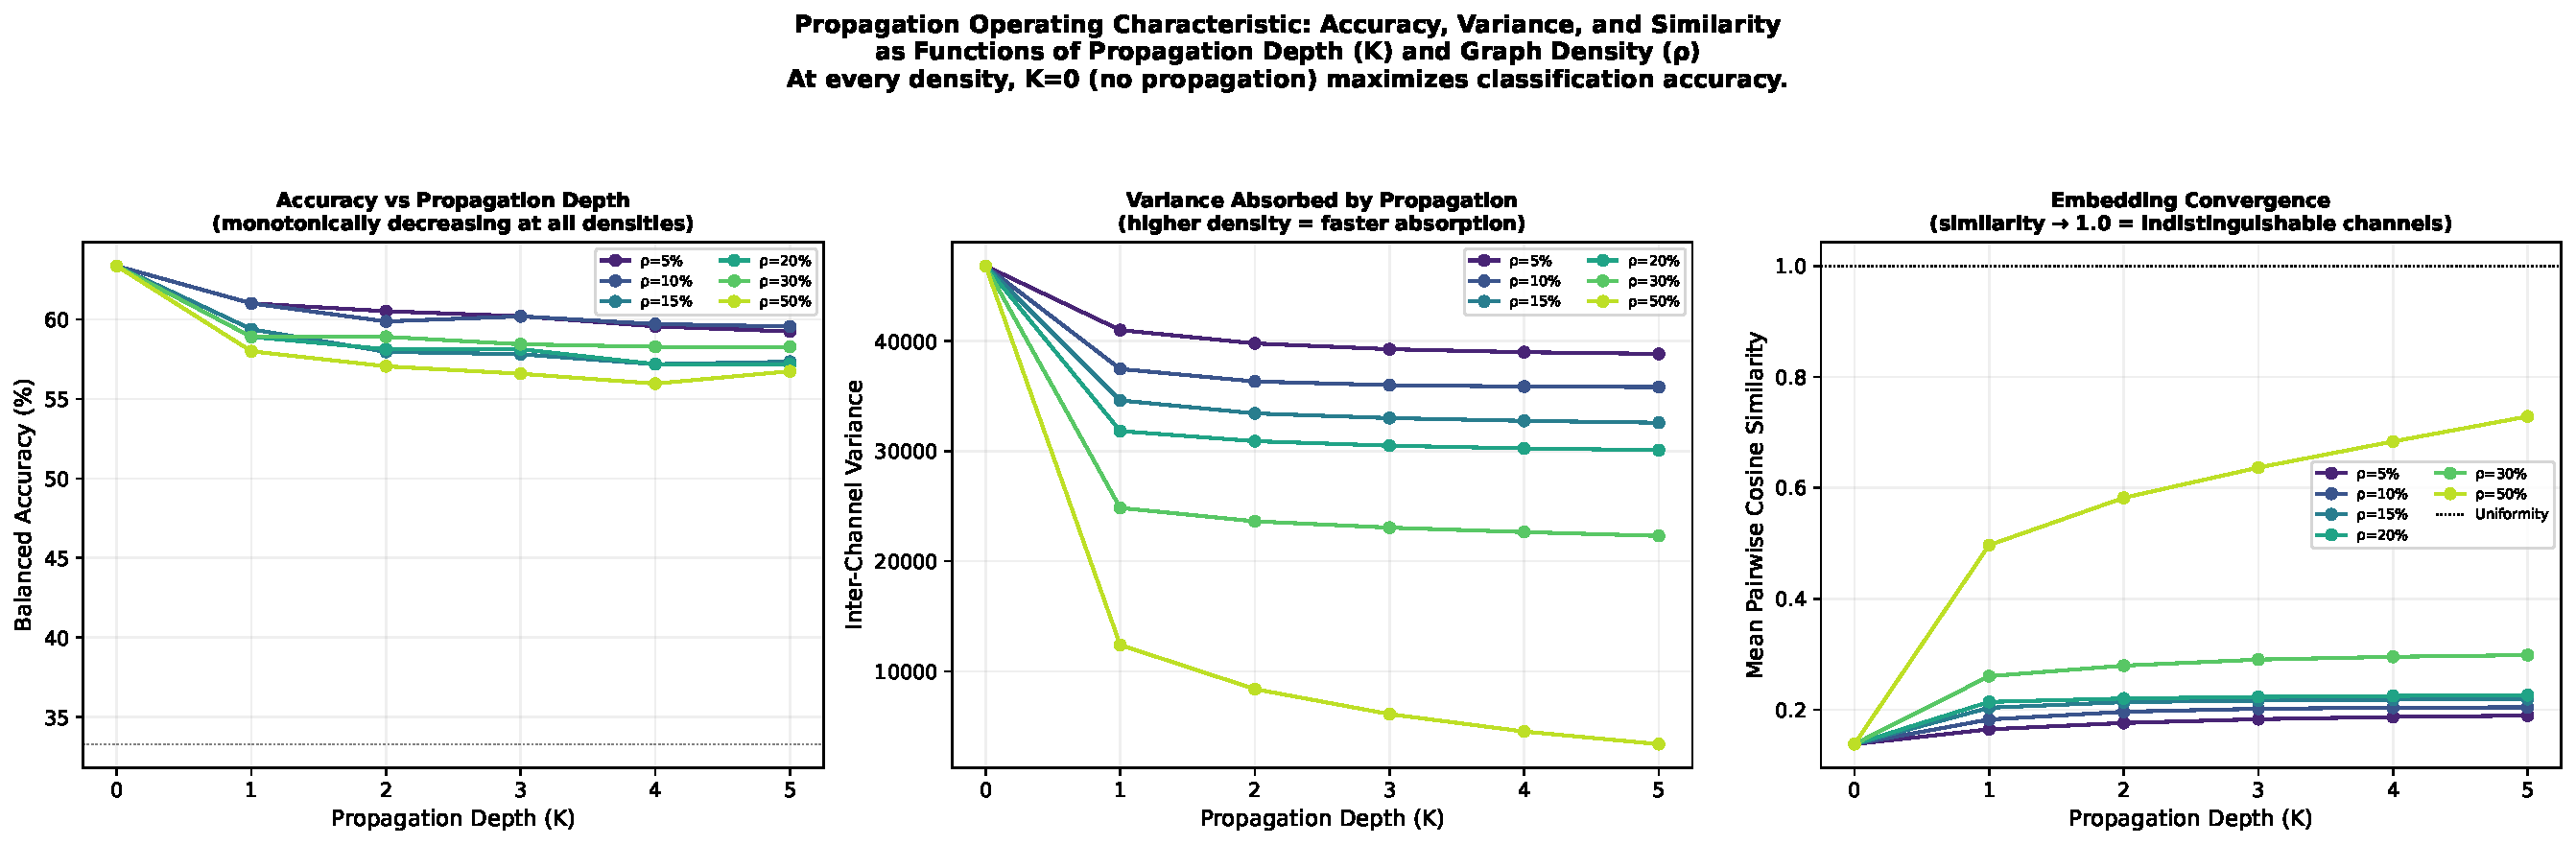
\includegraphics[width=\textwidth]{pictures/chGraphNeuralNetworks/exp03_propagation_operating_characteristic.pdf}
    \caption{Archived propagation sweep ($6$ densities $\times$ $6$ depths). Within these runs, the displayed accuracy decreases with depth, inter-channel variance decreases, and cosine similarity increases. PCA was fitted globally, so values are descriptive legacy estimates.}
    \label{fig:exp03_poc}
\end{figure}

Three observations emerge. First, classification accuracy is \emph{monotonically decreasing} in $K$ at every density tested. The maximum accuracy is always at $K = 0$ (no propagation). At $\rho = 20\%$, two layers reduce accuracy from $63.4\%$ to $58.1\%$; at $\rho = 50\%$, from $63.4\%$ to $57.0\%$.

Second, inter-channel variance decreases monotonically with $K$, and the rate of decrease accelerates with density. At $\rho = 20\%$ and $K = 2$, variance drops by $34\%$; at $\rho = 50\%$ and $K = 4$, by $90\%$. This quantifies the smoothing mechanism: each propagation layer absorbs inter-channel discriminative contrast.

Third, pairwise cosine similarity increases monotonically with $K$, from $0.138$ at $K = 0$ to $0.684$ at $\rho = 50\%$, $K = 4$, indicating that channel embeddings converge toward a common profile. The channel identity that carries the classification signal is progressively erased.

\subsection{Graph Construction Sweep}

Figure~\ref{fig:exp04_sweep} compares the archived estimate under three adjacency constructions: thresholded PCA-coordinate similarity, an assumed spatial-distance graph, and a degree-matched random graph. All three displayed $K=2$ values are lower than the $K=0$ comparison. The channel montage used for the spatial graph was not verified.

All three tested constructions produce lower archived accuracy than the non-propagated comparison. This shows that none improved that implementation; it does not demonstrate that graph size or density is the cause. In particular, the Pearson graph is a feature-similarity construction and, given the PCA-basis limitation described above, should not be called a physiological functional-connectivity graph.

\begin{figure}[H]
    \centering
    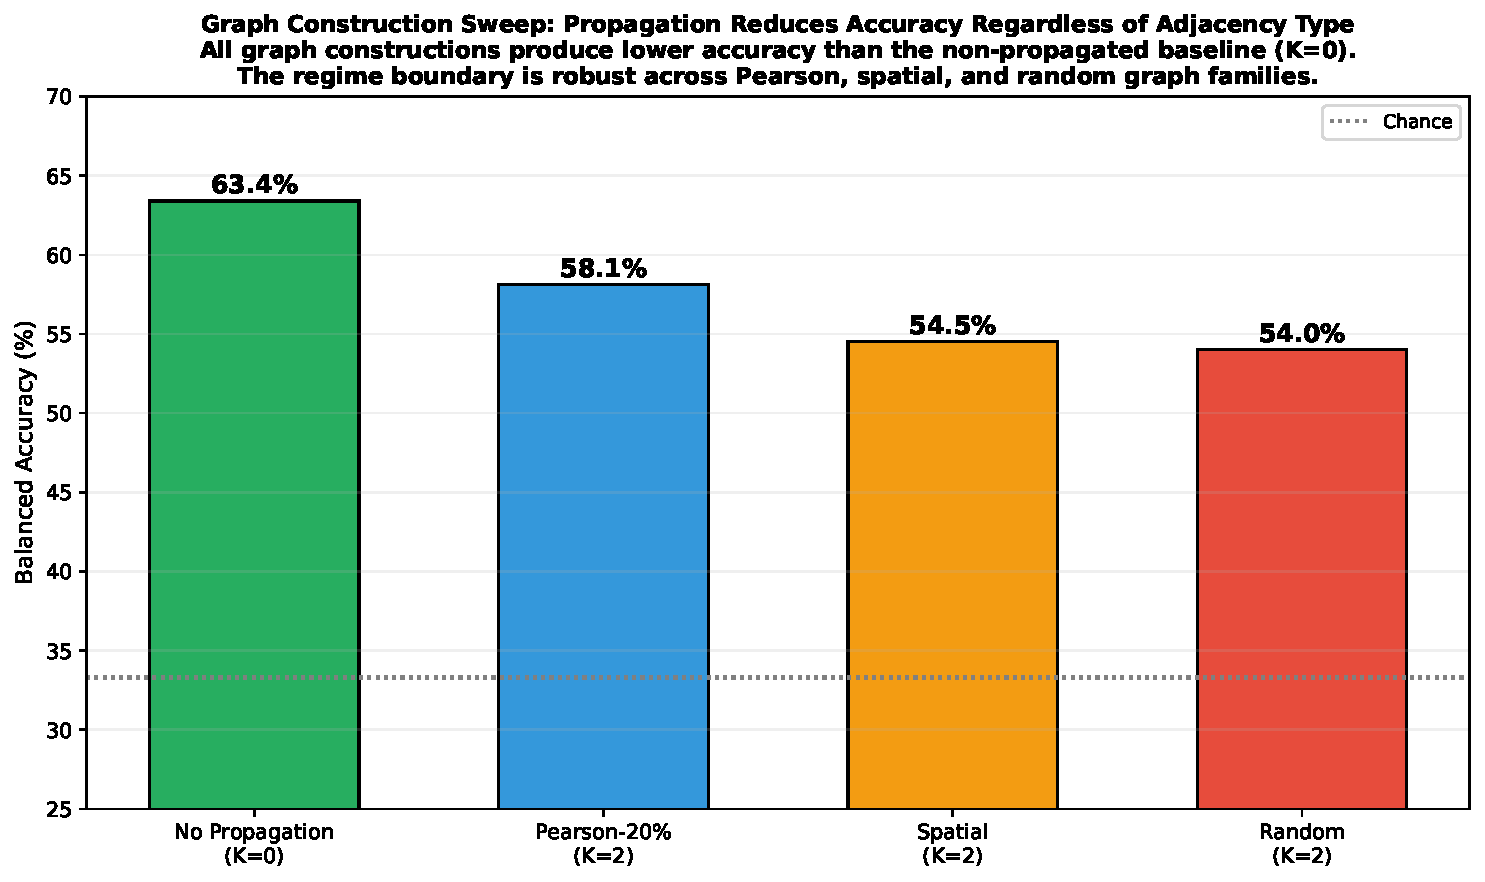
\includegraphics[width=\textwidth]{pictures/chGraphNeuralNetworks/exp04_graph_construction_sweep.pdf}
    \caption{Archived graph-construction sweep. The tested Pearson-similarity, assumed-spatial, and random constructions produce lower displayed accuracy at $K=2$ than the $K=0$ comparison. The montage used for the spatial construction was not verified.}
    \label{fig:exp04_sweep}
\end{figure}

\subsection{Heterophily-Aware and Contrast-Preserving Graph Operators}

The observation that standard smoothing-based message-passing reduces accuracy raises a natural question: do contrast-preserving graph operators recover or exceed the non-propagated baseline? The smoothing hypothesis predicts that operators designed to preserve or amplify inter-channel differences should avoid the variance-absorption mechanism observed in standard GCN propagation. Four contrast-preserving operator families were evaluated (Figure~\ref{fig:exp06_operators}).

\begin{figure}[H]
    \centering
    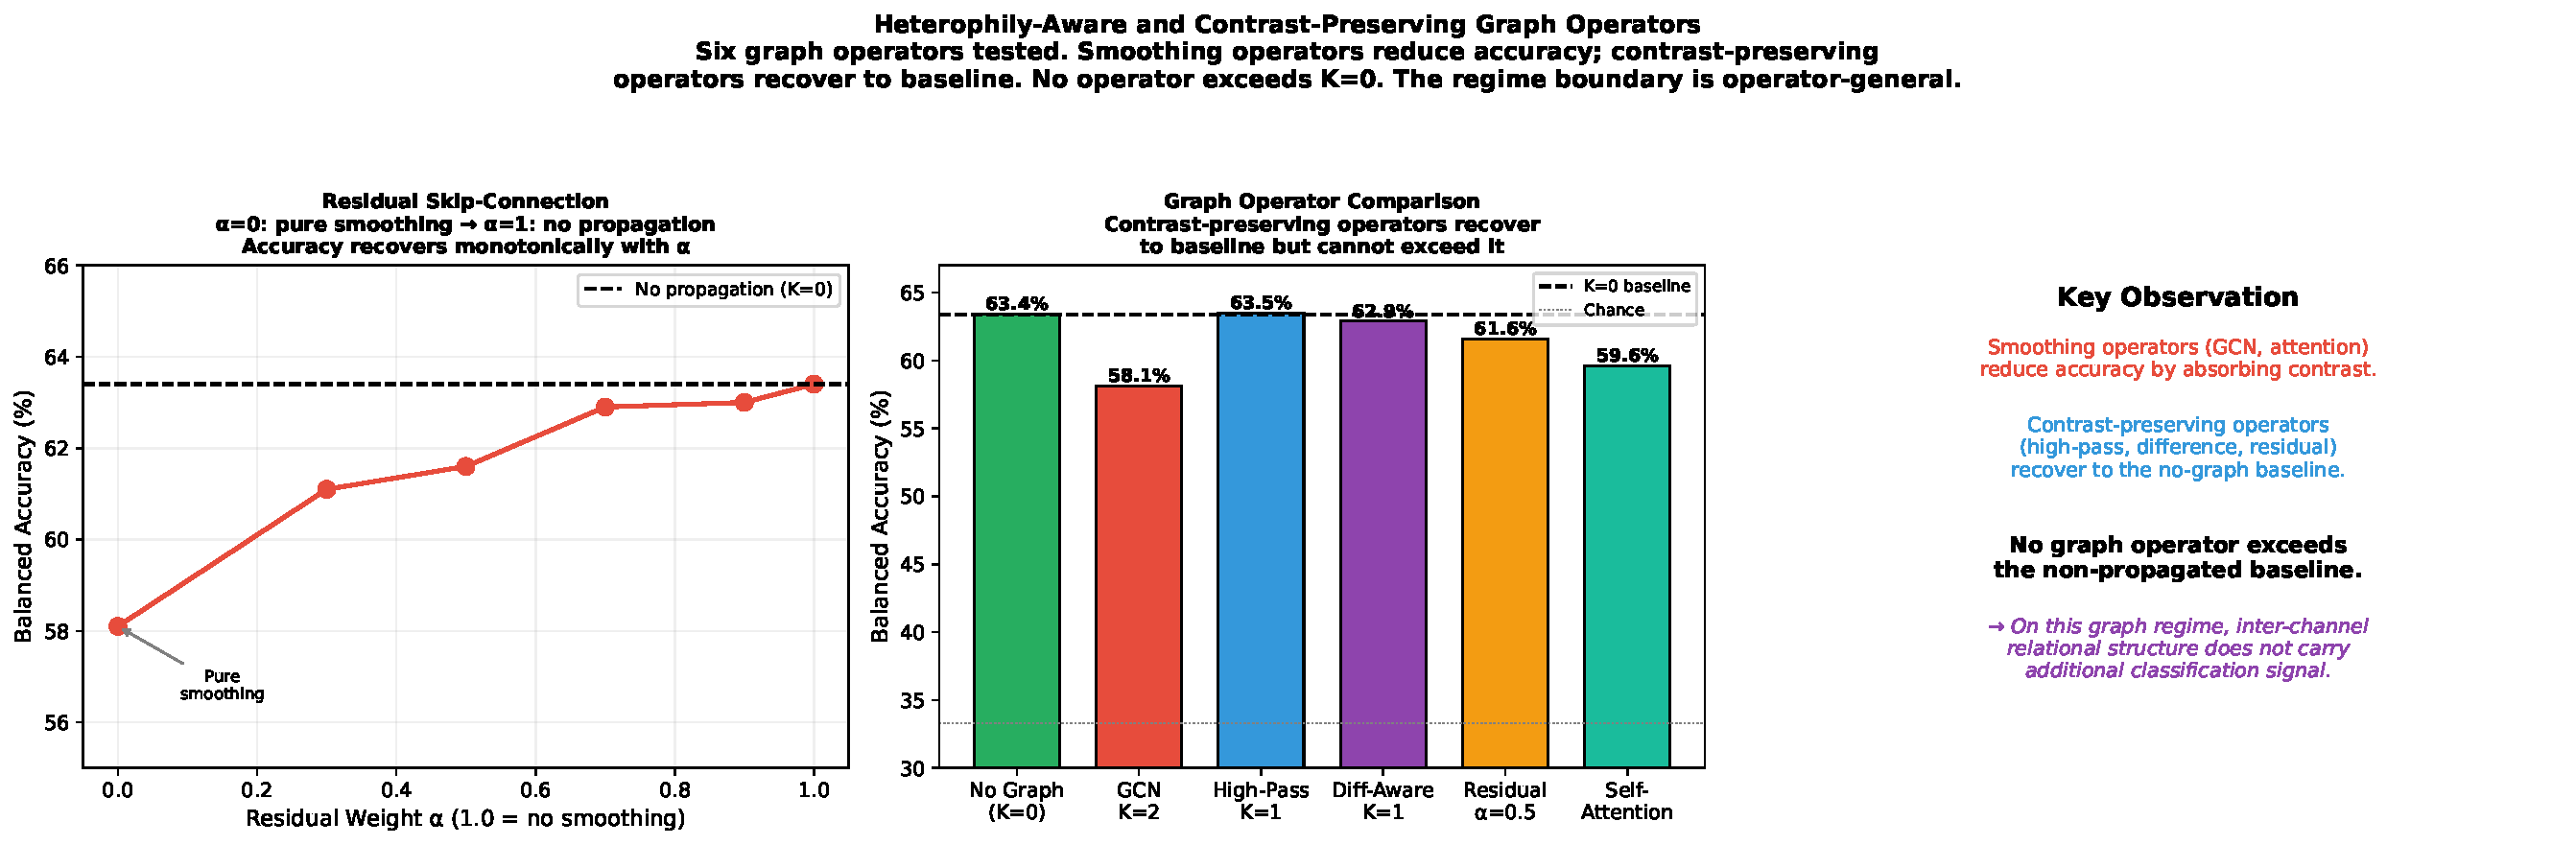
\includegraphics[width=\textwidth]{pictures/chGraphNeuralNetworks/exp06_heterophily_operators.pdf}
    \caption{Archived graph-operator analysis. Left: residual skip-connection sweep, from pure smoothing ($\alpha=0$) to no propagation ($\alpha=1$). Center: the tested contrast-preserving operators approach the $K=0$ comparison. Right: summary of the measured values.}
    \label{fig:exp06_operators}
\end{figure}

\textbf{Residual skip-connection} ($\mathbf{H}^{(k+1)} = \alpha \mathbf{H}^{(0)} + (1-\alpha)\hat{\mathbf{A}}\mathbf{H}^{(k)}$): the archived point estimate increases with $\alpha$, from $58.1\%$ at $\alpha = 0$ to $63.4\%$ at $\alpha = 1$. The largest displayed value is therefore the identity, or no-propagation, endpoint; no nested selection test establishes a generally optimal setting.

\textbf{High-pass graph filter} ($\mathbf{H}^{(k+1)} = (2\mathbf{I} - \hat{\mathbf{A}})\mathbf{H}^{(k)}$): amplifies differences between neighboring channels rather than smoothing them. Achieves $63.5\%$ at $K = 1$, matching the baseline within noise.

\textbf{Signed-difference aggregation} (aggregate $|\mathbf{h}_i - \mathbf{h}_j|$ across neighbors): achieves $62.9\%$ at $K = 1$, again matching the baseline.

\textbf{Channel self-attention} (softmax attention across all channels, no graph constraint): achieves $59.6\%$, below the baseline, indicating that even learned attention weights absorb discriminative contrast on this small array.

In the archived comparisons, smoothing operators reduce accuracy and the contrast-preserving variants approach, but do not clearly exceed, the non-propagated result. Seven named operator families were considered (GCN, GIN, EdgeConv, high-pass, residual, difference-aware, and self-attention). This is evidence about the tested configurations only; it does not establish that all inter-channel relational structure is uninformative.


\section{Exploratory Graph-Topological Associations}
\label{sec:ch5_interpretability}

The graph summaries were screened against multiple clinical variables, node metrics, edges, and interaction terms. These analyses were not prespecified as a single confirmatory family. Unless an adjustment is stated, the $p$ values below are nominal; with many comparisons, some $p<0.05$ results are expected under the null. The strongest nominal SUD comparison does not reach $p<0.05$ in its label-permutation check. Accordingly, this section reports exploratory cohort associations and makes no phenotype or biomarker claim.

\subsection{Graph-Level Associations}

GAD has the only nominal graph-level association in this screen: participants with GAD ($n=60$) have greater degree heterogeneity in the archived graph ($d=+0.34$, nominal $p=0.032$). This result is uncorrected and does not establish a population association.

\subsection{Channel-Level Clinical Comparisons}

The uncorrected channel-level screen contains nominal $p<0.05$ comparisons for each clinical variable (Figure~\ref{fig:channel_biomarkers}). Counts of nominal results cannot be interpreted without the size and dependence structure of the tested family. Examples include Ch14 clustering for MDD ($d=-0.45$, nominal $p=0.003$), Ch3 clustering for PTSD ($d=+0.36$, nominal $p=0.011$), and several channel-strength comparisons for SUD. Because the channels are unlabeled, the PCA bases in the archived graph are not commensurate, and family-wise inference was not established, these observations do not support anatomical or connectivity interpretations.

\begin{figure}[H]
    \centering
    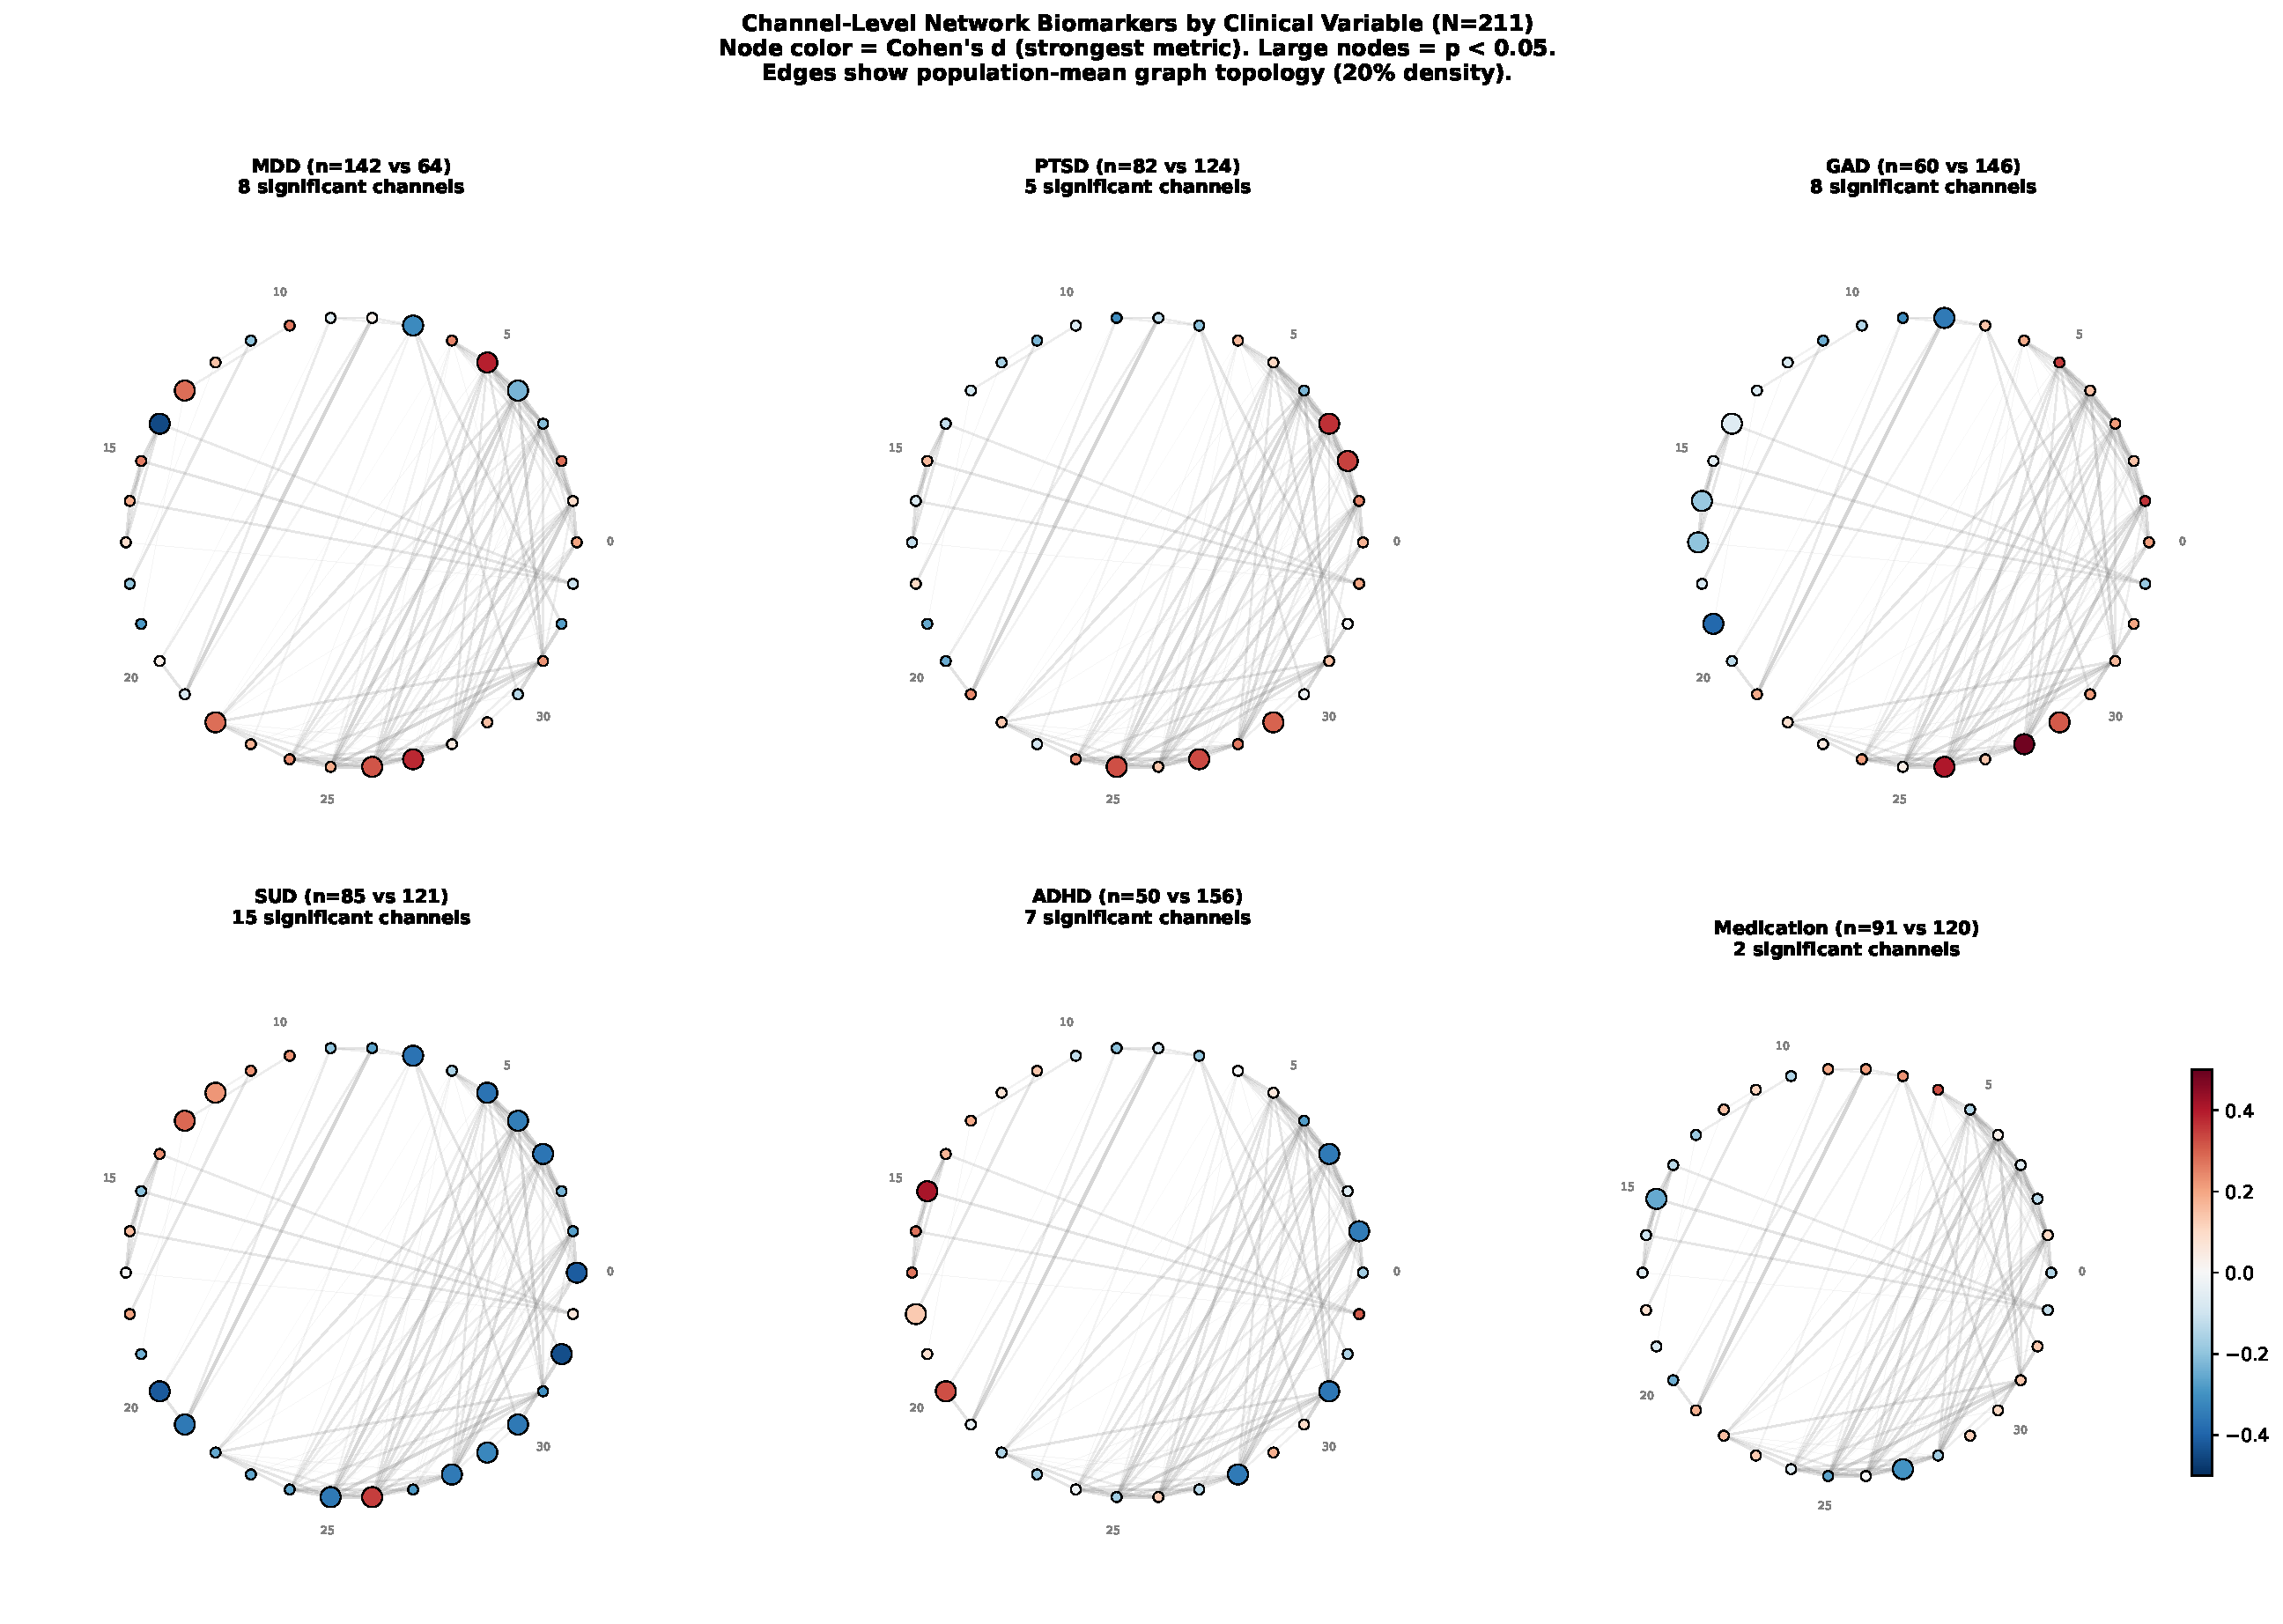
\includegraphics[width=\textwidth]{pictures/chGraphNeuralNetworks/fig_channel_biomarkers_211.pdf}
    \caption{Exploratory channel-level graph comparisons ($N=211$). Node color shows the largest displayed Cohen's $d$ and larger nodes mark nominal $p<0.05$. Results are uncorrected and channels are unlabeled.}
    \label{fig:channel_biomarkers}
\end{figure}

\subsection{Substance Use Disorder Screen}
\label{ssec:ch5_sud}

The smallest nominal $p$ value in the archived clinical screen occurs in an SUD reactivity comparison (Figure~\ref{fig:sud_interactions}). Three reported comparisons are summarized below, without confirmatory interpretation.

\textbf{SUD $\times$ Strength reactivity (nominal $p=0.0004$).} The parametric summary reports $d=-0.52$, with mean changes of $+0.037$ for the non-SUD group and $-0.023$ for the SUD group. The separate permutation output reports $d=-0.34$. The archived materials do not document enough detail to reconcile these effect-size estimates, so neither is treated as a definitive estimate.

\textbf{SUD $\times$ Efficiency reactivity (nominal $p=0.003$, $d=+0.43$).} The displayed group means change in opposite directions. Because the test is part of an exploratory family and uses the archived graph, the difference is not assigned a mechanistic interpretation.

\textbf{SUD $\times$ Clustering reactivity (nominal $p=0.012$, $d=-0.35$).} The displayed group means again change in opposite directions; this is an uncorrected descriptive comparison.

The three directions appear visually coherent, but they were selected from a larger screen and do not establish a coherent disorder mechanism. Comorbidity, medication, and other confounding were not isolated, and the graph values cannot be interpreted as direct neural connectivity.

For the SUD strength comparison, $5{,}000$ label permutations yield an empirical $p=0.073$ (Figure~\ref{fig:exp05_permutation}). The test therefore does not reject the permutation null at $\alpha=0.05$. The nominal parametric result is retained only as a hypothesis for future, prespecified analysis.

\begin{figure}[H]
    \centering
    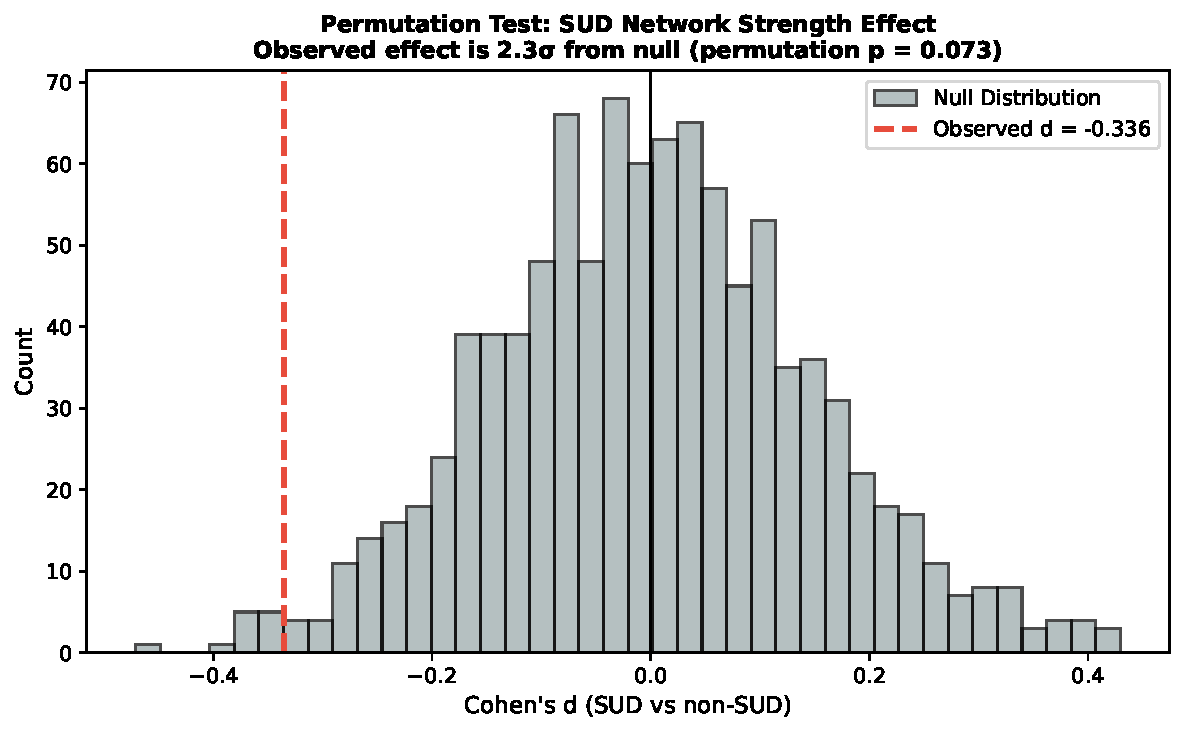
\includegraphics[width=0.55\textwidth]{pictures/chGraphNeuralNetworks/exp05_permutation_test.pdf}
    \caption{Permutation test for the SUD network strength effect. The observed effect (red dashed) is $2.3$ null standard deviations from the permutation mean, but the empirical permutation test does not reach significance ($p = 0.073$; $5{,}000$ permutations).}
    \label{fig:exp05_permutation}
\end{figure}

\begin{figure}[H]
    \centering
    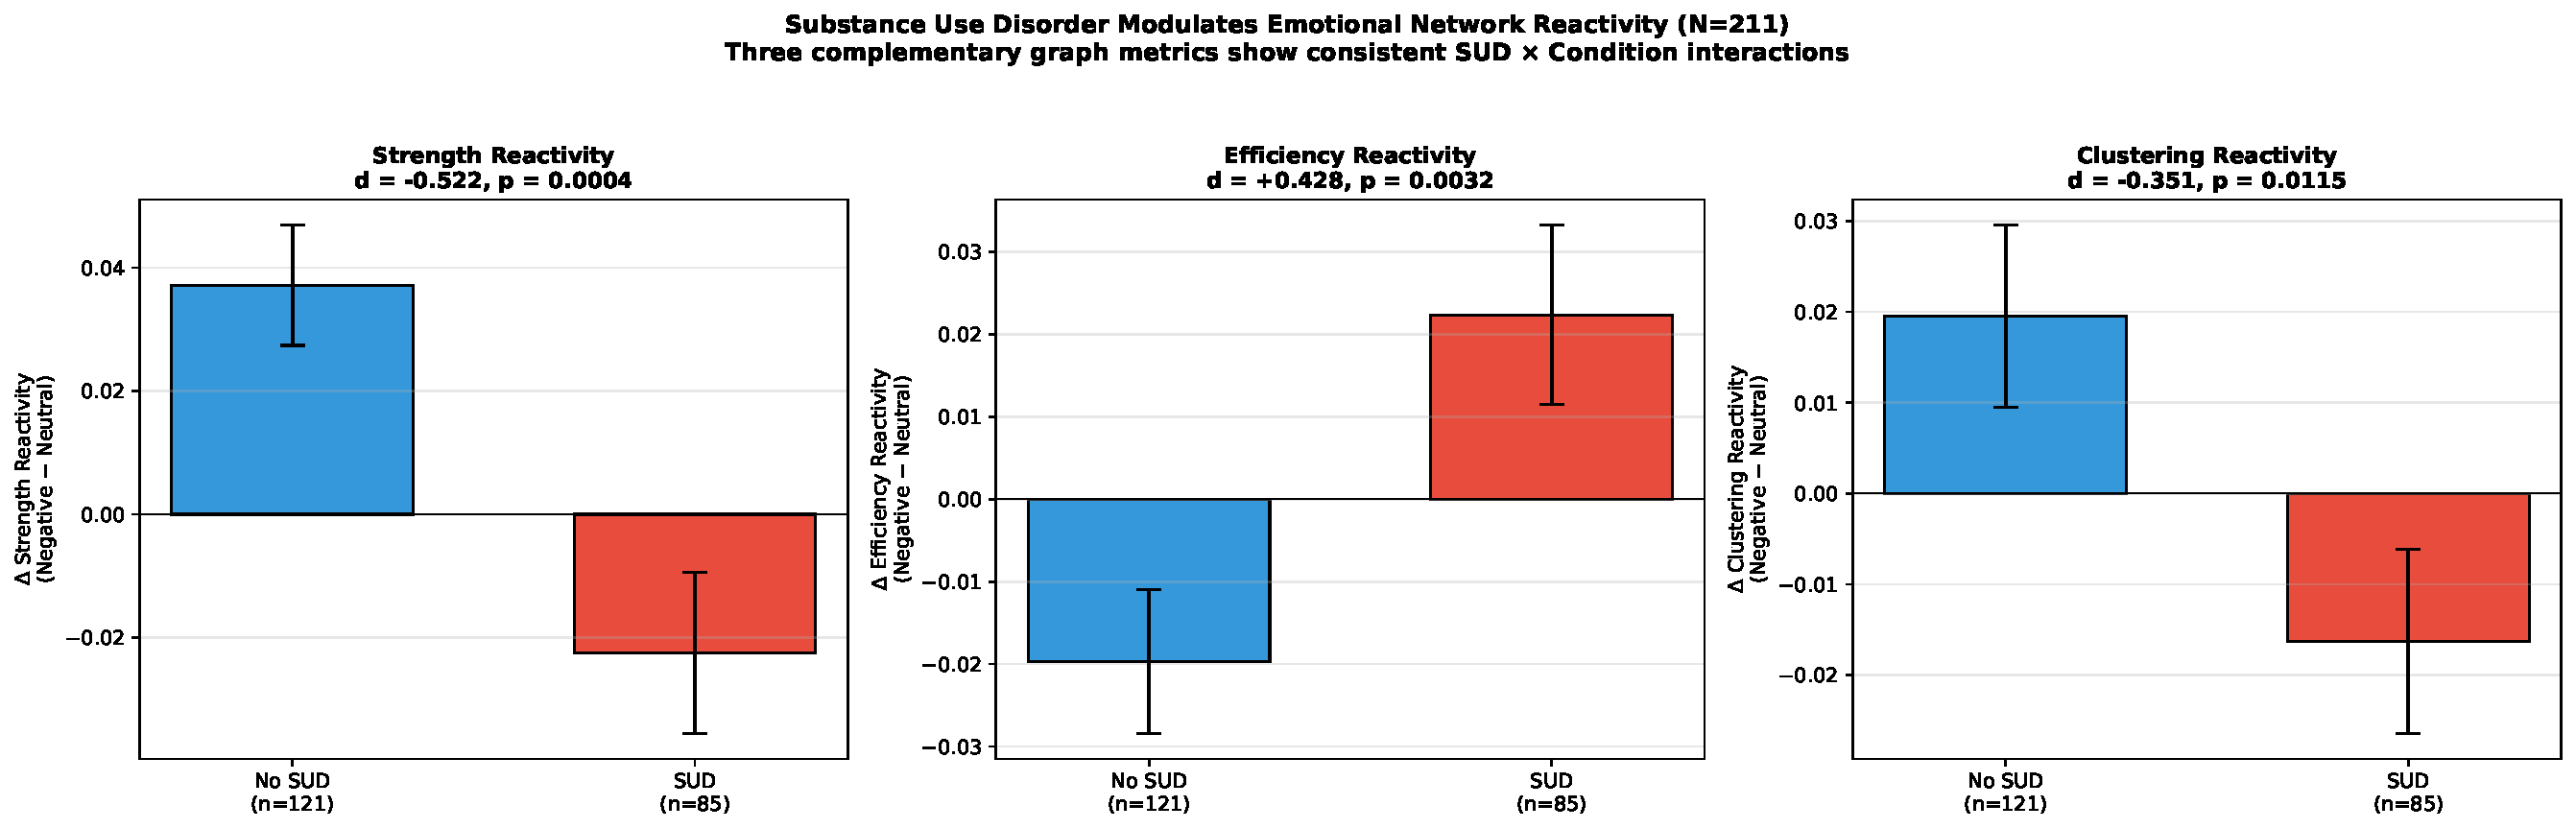
\includegraphics[width=\textwidth]{pictures/chGraphNeuralNetworks/fig_sud_interactions_211.pdf}
    \caption{Exploratory SUD reactivity comparisons for three archived graph summaries. The directions differ between groups; the strongest comparison has empirical permutation $p=0.073$. Error bars show SEM.}
    \label{fig:sud_interactions}
\end{figure}

\subsection{Additional Interaction Effects}

Two additional nominal interactions are GAD $\times$ efficiency reactivity ($d=-0.32$, $p=0.032$) and sex $\times$ strength reactivity ($d=+0.37$, $p=0.024$). Neither is multiplicity-adjusted, and six participants are absent from the binary sex counts; these comparisons are descriptive.

\subsection{Nested-Sample Stability Check}
\label{sec:ch5_nonrep}

Two nominal interactions from the initial $N=115$ subset were re-examined in the overlapping $N=211$ sample (Figure~\ref{fig:nonreplication}): medication $\times$ efficiency reactivity and PTSD $\times$ clustering reactivity. Neither has nominal $p<0.05$ in the larger sample. A change in significance does not itself establish that an effect is absent or sample-specific; effect estimates and uncertainty, not the dichotomy alone, should guide interpretation.

Because the samples overlap, this check is not an independent replication and cannot estimate reproducibility. It records how selected estimates changed when additional observations were added. All clinical-label findings require independent, prespecified evaluation with multiplicity control.

\begin{figure}[H]
    \centering
    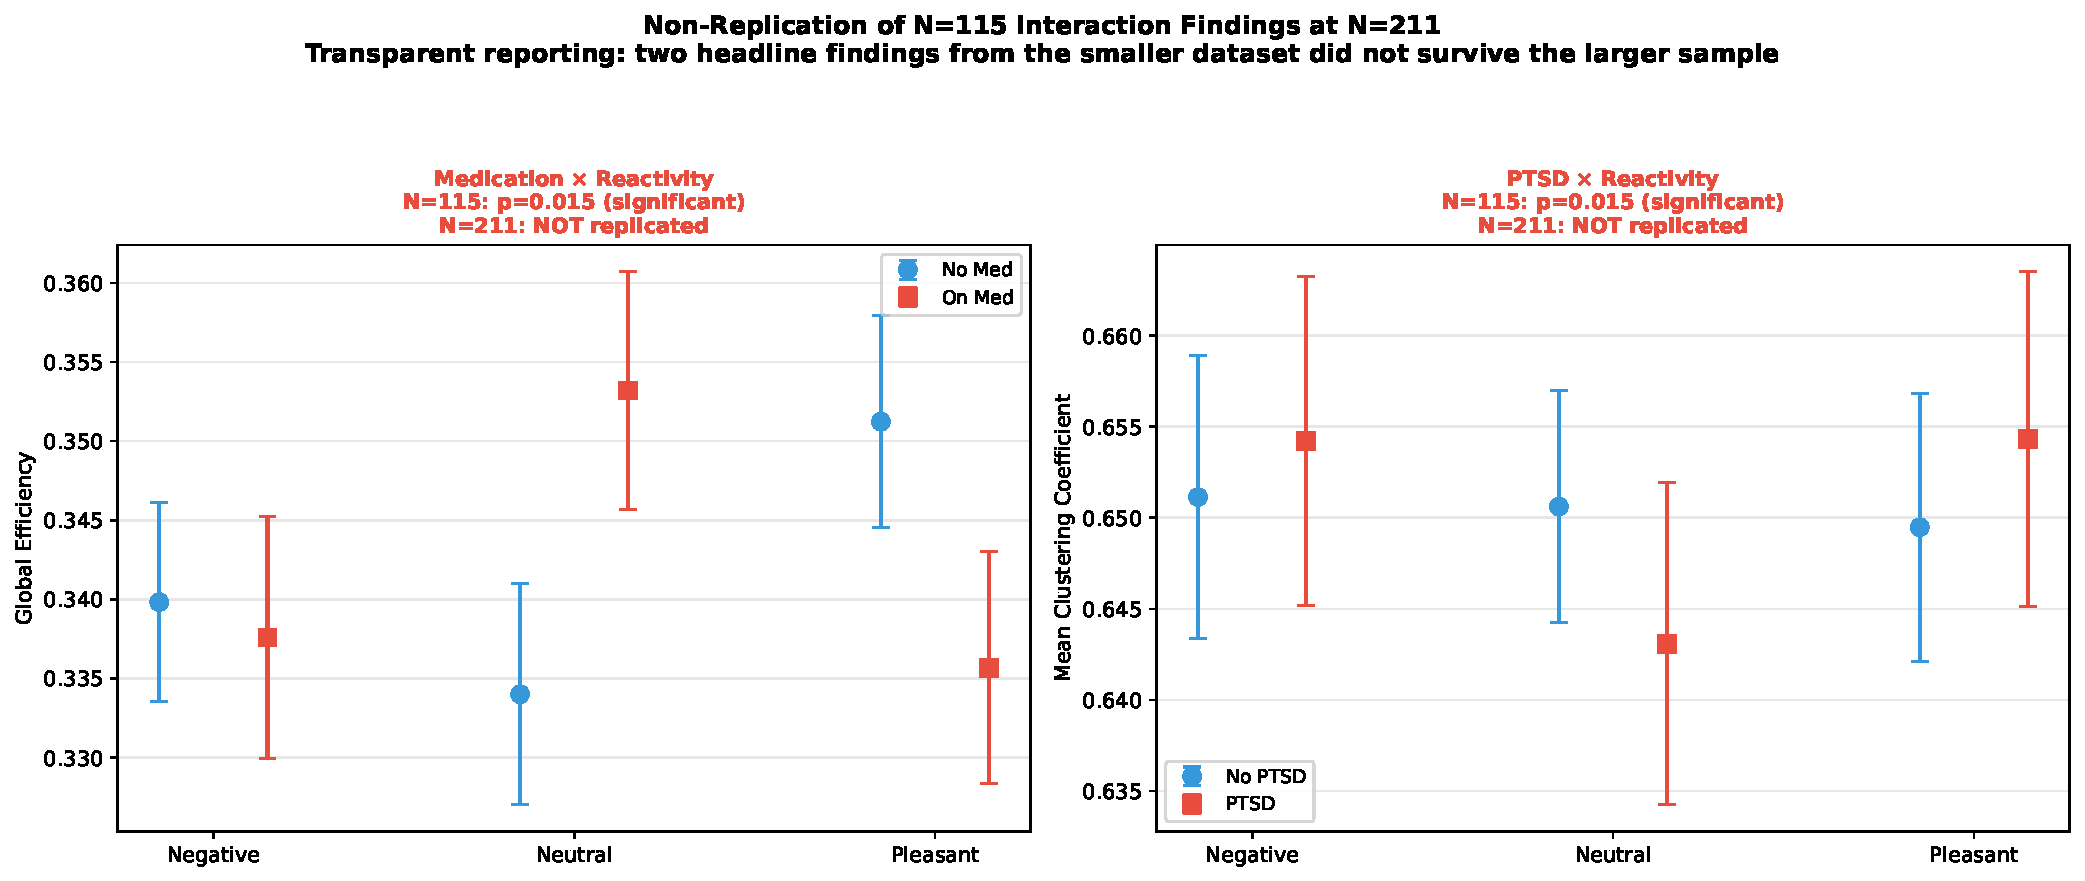
\includegraphics[width=\textwidth]{pictures/chGraphNeuralNetworks/fig_nonreplication_211.pdf}
    \caption{Nested-sample stability check for two exploratory interactions. The $N=115$ sample is contained within the $N=211$ sample, so this is not an independent replication.}
    \label{fig:nonreplication}
\end{figure}

\subsection{Edge-Level Comparisons}

No clinical variable produced edges surviving FDR correction (Figure~\ref{fig:edge_biomarkers}); the analysis therefore does not isolate any edge-level clinical association after multiplicity control. For PTSD, Ch0$\leftrightarrow$Ch27 is the strongest uncorrected single-edge effect ($d = +0.43$, $p = 0.003$), consistent with its ranking in the $N = 115$ analysis. Because the electrodes are unlabeled and the result does not survive FDR correction, anatomical or biomarker interpretation is not supported.

\begin{figure}[H]
    \centering
    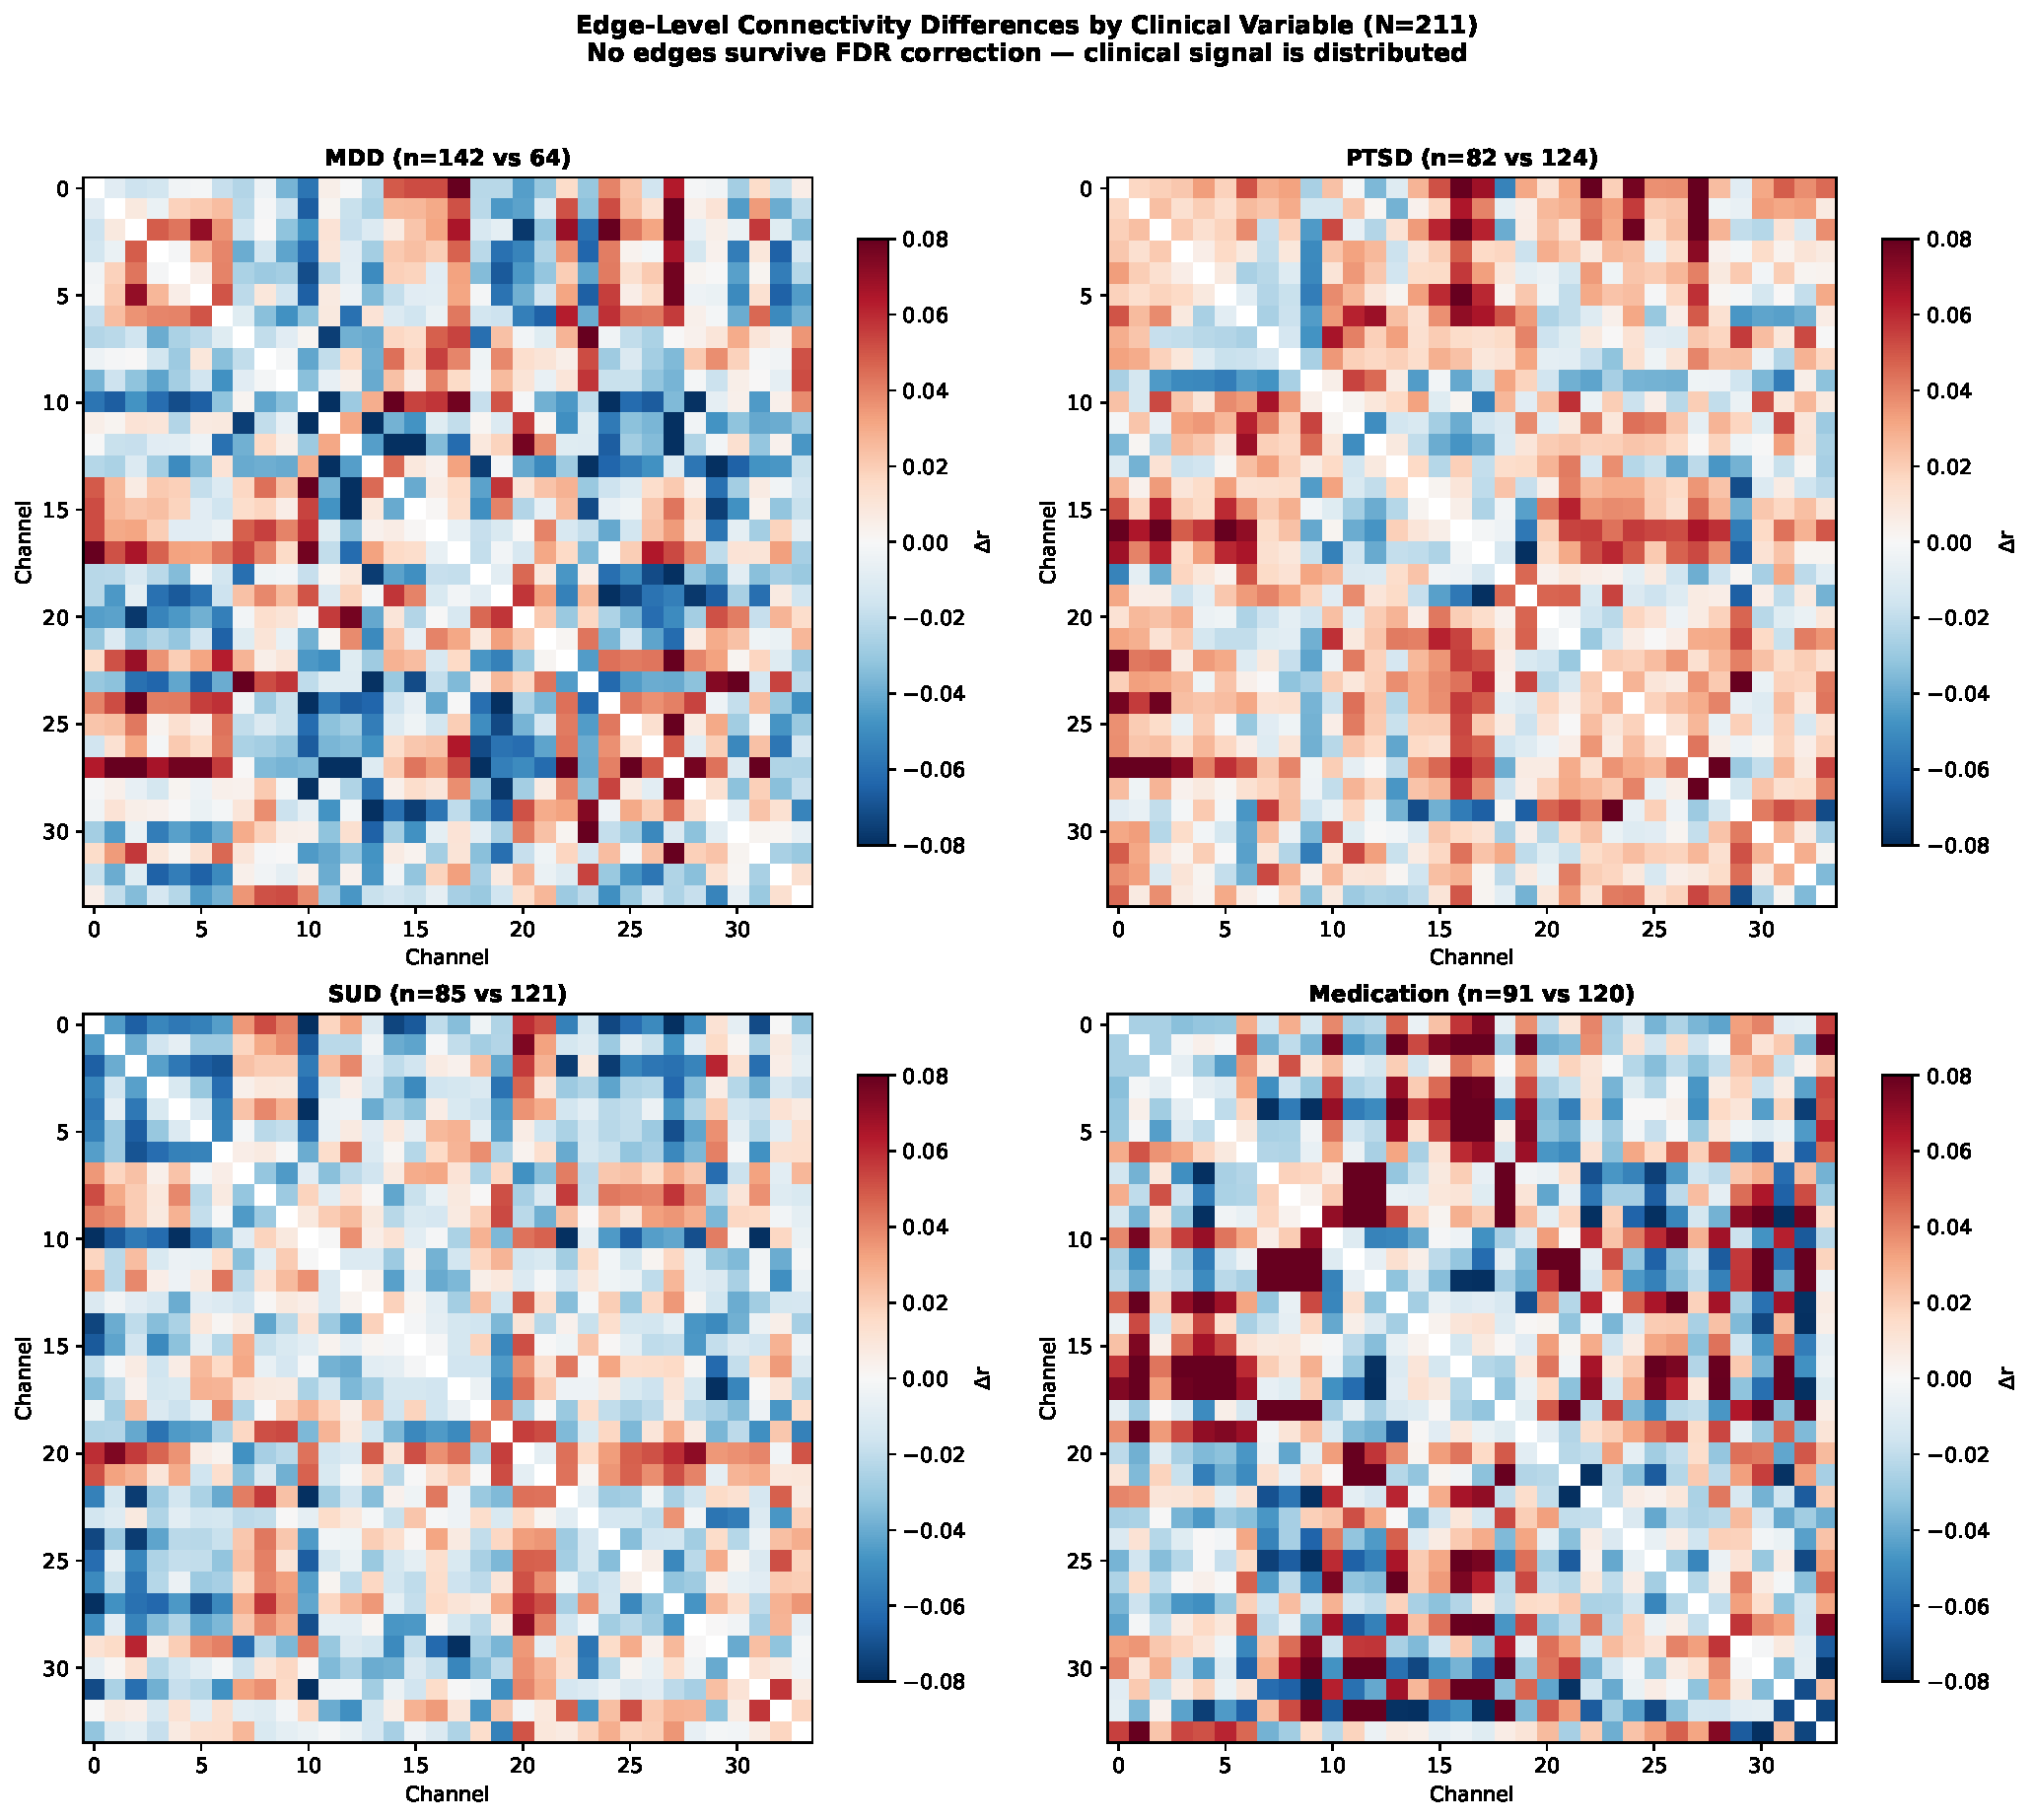
\includegraphics[width=\textwidth]{pictures/chGraphNeuralNetworks/fig_edge_biomarkers_211.pdf}
    \caption{Exploratory edge-level differences ($N=211$). No tested edge survives FDR correction.}
    \label{fig:edge_biomarkers}
\end{figure}


\section{Descriptive Comparison Across Label Granularities}
\label{sec:ch5_4class}

The archived project also analyzes four labels (Threat, Mutilation, Cute, and Erotic) for the same $211$ participants. The three- and four-class scripts do not implement a controlled one-factor comparison: they differ in the number of observations, class definitions, and details of PCA/feature processing. Both also use global PCA for the displayed results. The following numerical contrast is therefore descriptive and cannot isolate the causal effect of label granularity.

\subsection{Observed Performance Difference}

Table~\ref{tab:regime_comparison} records the displayed differences. In the three-class run, the reservoir estimate is $12.5$ percentage points above band-power; in the four-class run, it is $6.2$ points below band-power. Because the pipelines are not otherwise identical and preprocessing was not fold-safe, this reversal is a hypothesis to test, not an identified regime boundary.

\begin{table}[t]
\centering
\caption{Archived cross-granularity results. The runs differ in class structure and preprocessing details; values are descriptive and do not identify a causal regime transition.}
\label{tab:regime_comparison}
\small
\renewcommand{\arraystretch}{1.15}
\begin{tabular}{lcc}
\hline
\textbf{Quantity} & \textbf{3-class} & \textbf{4-class} \\
\hline
Number of classes & 3 & 4 \\
Best raw classifier & Reservoir + SVM & BandPower + SVM \\
Best raw balanced accuracy & $63.4\%$ & $40.4\%$ \\
Best centered accuracy & $79.4\%$ & $52.0\%$ \\
Subject-centering gain & $+16.0$ pp & $+10.8$ pp \\
Band-power accuracy & $50.9\%$ & $40.4\%$ \\
Reservoir $>$ BandPower? & Yes ($+12.5$ pp) & No ($-6.2$ pp) \\
GNN beats non-propagated? & No & No \\
Subject variance fraction & $62.6\%$ & $47.0\%$ \\
Condition variance fraction & $8.7\%$ & $2.4\%$ \\
Subject / condition ratio & $7.2\times$ & $19.6\times$ \\
Smallest nominal clinical $p$ & SUD $p = 0.0004$ & PTSD $p = 0.036$ \\
\hline
\end{tabular}
\end{table}

The archived variance decompositions assign $8.7\%$ to condition in the three-class representation and $2.4\%$ in the four-class representation. These decompositions were fitted to different design matrices and globally transformed feature spaces. They are compatible with weaker class separation in the four-class run, but they do not explain its cause or prove that temporal binning lacks the required resolution.

\subsection{Pairwise Accuracy Pattern}

In the archived pairwise results, Cute versus Erotic has the highest displayed accuracy ($69.0\%$), while Threat versus Cute has the lowest ($52.8\%$). An arousal account is plausible, but stimulus-level valence/arousal scores were not modeled here and the pairwise contrasts differ in more than one property. The result therefore does not establish that the reservoir is more sensitive to arousal than valence.

\subsection{Four-Class Clinical Findings}

In the four-class screen, PTSD has $11$ nominal channel--metric comparisons and $28$ nominal edge comparisons, and a PTSD $\times$ Threat--Mutilation term has nominal $p=0.036$. These counts and $p$ values are uncorrected. The SUD $\times$ global-efficiency term has nominal $p=0.008$, but a result from the same participants under a different labeling does not provide independent replication. Neither comparison supports a disorder signature.

The identity of the smallest nominal $p$ value differs across the two screens. Given the number of comparisons, overlapping sample, and pipeline differences, this ordering should not be interpreted as evidence that different disorders are detectable at different emotional resolutions.


\section{Layer Ablation and Complementarity Analysis}
\label{sec:ch5_ablation}

The preceding sections define an embedding block (E), a dynamical-summary block (D), a graph-summary block (T), and a coupling summary (C). This section compares their archived cross-validation estimates using $L_2$-regularized logistic regression. The comparison was not nested around all feature-selection and preprocessing decisions, so it is descriptive rather than a confirmatory test of complementarity.

\subsection{Emotion Classification Ablation}

Table~\ref{tab:emotion_ablation} presents the A1--A9 results on the three-class task. The largest displayed estimate is for the embedding-containing blocks, while topology and coupling are near chance. No nested model-comparison test or held-out selection procedure was used to establish differences among the close estimates. The table therefore ranks the archived point estimates but does not confirm that one block adds information beyond another.

\begin{table}[t]
\centering
\caption{Archived feature-block comparison for three-class classification (logistic regression, 10 subject-grouped folds). E~$=$~BSC$_6$/PCA-64 embedding; D~$=$~dynamical summaries; T~$=$~graph summaries; C~$=$~coupling scalar. PCA-dependent values use the earlier global-PCA pipeline.}
\label{tab:emotion_ablation}
\small
\begin{tabular}{llcc}
\hline
\textbf{ID} & \textbf{Features} & \textbf{Dim} & \textbf{Bal.\ Accuracy} \\
\hline
A0 & BandPower & 170 & $49.4 \pm 5.1\%$ \\
A1 & E & 2,176 & $59.4 \pm 3.6\%$ \\
A2 & D & 238 & $42.2 \pm 6.0\%$ \\
A3 & T & 68 & $35.3 \pm 4.7\%$ \\
A4 & C & 3 & $35.4 \pm 6.9\%$ \\
A5 & D + T & 306 & $43.8 \pm 7.2\%$ \\
A6 & E + D & 2,414 & $59.3 \pm 4.5\%$ \\
A7 & E + T & 2,244 & $60.1 \pm 4.3\%$ \\
A8 & E + D + T & 2,482 & $59.7 \pm 3.9\%$ \\
A9 & E + D + T + C & 2,485 & $59.4 \pm 3.8\%$ \\
\hline
\end{tabular}
\end{table}

In the RBF-SVM sensitivity run, E is $62.1\%$, D is $49.8\%$, and T shows no increase. This similar ordering is a descriptive sensitivity observation, not an independent confirmation.

\subsection{Clinical Detection Ablation}

The clinical-label estimates in Table~\ref{tab:clinical_ablation} range from $37.9\%$ to $53.8\%$ balanced accuracy and are mostly close to chance. The bold entries select the maximum within each diagnosis after observing the results; no nested selection, permutation test, or uncertainty interval establishes that those maxima differ from chance or from the other blocks. They should not be read as disorder-detection performance.

\begin{table}[t]
\centering
\caption{Exploratory clinical-label feature-block comparison (logistic regression, five subject-grouped folds). The maximum point estimate per label is bold; maxima were selected post hoc and do not establish layer-specific clinical sensitivity.}
\label{tab:clinical_ablation}
\small
\begin{tabular}{lccccc}
\hline
\textbf{ID} & \textbf{SUD} & \textbf{MDD} & \textbf{PTSD} & \textbf{GAD} & \textbf{ADHD} \\
\hline
C1 (E) & $50.9\%$ & $48.9\%$ & $45.2\%$ & $50.6\%$ & $52.8\%$ \\
C2 (D) & $\mathbf{53.6\%}$ & $44.6\%$ & $50.6\%$ & $50.2\%$ & $46.3\%$ \\
C3 (T) & $42.1\%$ & $48.6\%$ & $48.2\%$ & $51.1\%$ & $37.9\%$ \\
C4 (D+T) & $52.1\%$ & $43.9\%$ & $\mathbf{52.6\%}$ & $46.4\%$ & $46.4\%$ \\
C5 (E+D+T) & $48.5\%$ & $\mathbf{51.8\%}$ & $45.3\%$ & $50.0\%$ & $51.5\%$ \\
C6 (C) & $52.7\%$ & $49.7\%$ & $47.0\%$ & $\mathbf{53.8\%}$ & $\mathbf{53.0\%}$ \\
\hline
\end{tabular}
\end{table}

\subsection{Interpretation of the Feature Blocks}

For emotion labels, the embedding-containing blocks have the largest archived point estimates. For clinical labels, all maxima are weak and uncertain. The blocks are operationally different by construction because they summarize different quantities, but this ablation does not show that they carry unique clinical information or map to distinct disorder mechanisms.


\section{Engineering Interpretation}
\label{sec:ch5_novelty}

\subsection{Contributions and Limits}

This chapter documents class-geometry summaries, propagation sweeps, a subject-panel normalization analysis, a cross-granularity comparison, and feature-block ablations. The post-defense audit identified global PCA and incompatible per-channel PCA bases in the archived Chapter~5 workflow. Consequently, results that depend on those operations are preserved for transparency as descriptive legacy estimates. The clinical-label analyses are exploratory, and the strongest SUD permutation result is $p=0.073$.

\subsection{Significance for Electrical Engineering}

The Propagation Operating Characteristic provides a systematic way to compare graph operators on finite sensor arrays. Across the tested GCN, high-pass, residual, difference-aware, self-attention, and no-propagation variants, the non-propagated representation yields the strongest measured separability. The subject--condition shared-subspace result also cautions against assuming that PCA-based nuisance removal is lossless. The node-count and density thresholds observed here are hypotheses for other EEG and biosignal graphs, not general design laws for ECG, EMG, or fNIRS.

\subsection{Clinical Interpretation Limits}

The clinical screens suggest questions for a future study but do not support clinical electrophysiology conclusions. The graph quantities are derived from reservoir features, not direct measurements of brain-network connectivity; montage labels are unavailable; the strongest SUD comparison fails its permutation test; and the analysis does not show an advantage over a multiplicity-controlled spectral-feature alternative.

The panel-centering result illustrates that repeated observations from a held-out subject can be used to remove that subject's mean feature vector. It does not demonstrate a field-wide flaw or show that a biological ``subject-identity component'' has been isolated. Its relevance is limited to designs in which all required within-subject observations are available together.


\section{Scope and Future Directions}
\label{sec:ch5_scope}

Future work should begin with verified electrode labels and montage coordinates, fold-local common-basis dimensionality reduction, nested model selection, and a prespecified multiplicity plan. The corrected pipeline should be rerun on the raw SHAPE data and tested in an independent cohort before clinical interpretation. Longitudinal data would also be required to distinguish stable participant differences from session and condition effects.


\section{Empirical Investigation of Traceability}
\label{sec:ch5_interpretability_investigation}

This section examines which intermediate quantities can be inspected and related to predefined temporal windows. Inspectability is not equated with faithful causal explanation, clinical usefulness, or model correctness.

\subsection{Theoretical Context: Interpretability in Spiking Neural Networks}
\label{sec:interp_theory}

Spiking models expose discrete event traces, but those traces are not self-interpreting. Anatomically structured systems such as NeuCube can associate learned activity with supplied coordinates \cite{kasabov_neucube_2014,doborjeh_explainable_2021}, and attention mechanisms can provide temporal weights \cite{yao_attention_snn_2023}. In each case, fidelity and usefulness require empirical evaluation; the presence of spikes, coordinates, or attention weights alone does not establish an explanation \cite{kim_sam_2021}.

Published approaches include spike-based activation maps, prototype explanations, readout-weight analyses, and dynamical summaries \cite{kim_sam_2021,barnett_protopmed_2024,alao_discovering_2021,reservoir_pe_2022}. These methods answer different questions, and no result in this dissertation establishes that the present pipeline is more interpretable than a non-spiking alternative.

The present investigation therefore tests limited forms of temporal indexing and case-based summarization while recording their inferential limits.

\subsection{Archived PCA and Centering Result}
\label{sec:shared_subspace}

In the archived global-PCA representation, the tested linear models do not recover the selected ERP scalars after panel centering ($R^2\leq-0.04$), and the tested classifiers are near chance. This is a negative result for those transformations and models, not evidence that the representation contains no recoverable condition information.

The archived subspace calculation reports first-five principal angles of $0^\circ$. Exact zero angles in a globally fitted, high-dimensional sample representation can arise from shared or saturated sample subspaces and do not show that the underlying population effects are identical. Panel centering subtracts each subject's across-condition mean; it is not a projection that necessarily removes every condition contrast.

The negative result motivates examining pre-compression temporal features and rerunning PCA within each training fold. It does not identify PCA as the unique cause of lost traceability, because the archived comparison changes several operations and does not perform a causal ablation.

\subsection{Aggregate Associations with ERP Summaries}
\label{sec:erp_recovery}

This supplementary analysis uses a separate early-window extractor spanning $39$ to $273$~ms; it is not the archived full-epoch embedding used in the primary Chapter~5 tables. Its aggregate correlations with broader P300 ($250$--$500$~ms) and LPP ($500$--$800$~ms) scalar summaries are $r=0.65$ and $|r|=0.82$, respectively; the early-window BSC$_6$ spike-count correlations are $r=0.33$ and $|r|=0.23$. Because most of the P300 window and the entire LPP window lie outside the six-bin span, these correlations cannot be interpreted as recovery or temporal localization of those components. They are aggregate cohort associations whose computation requires independent verification.

A separate sweep compares three binning resolutions:
\begin{center}
\begin{tabular}{lcccc}
\toprule
\textbf{Bins} & \textbf{Resolution} & \textbf{Accuracy} & \textbf{Peak Bin} & \textbf{Concentration} \\
\midrule
6 & 39.1~ms & $67.0\% \pm 5.4\%$ & Bin 6 (234--273~ms) & 1.039 \\
12 & 19.5~ms & $65.9\% \pm 3.3\%$ & Bin 10 (176--195~ms) & 1.057 \\
24 & 7.8~ms & $63.5\% \pm 5.5\%$ & Bin 22 (172--180~ms) & 1.047 \\
\bottomrule
\end{tabular}
\end{center}
The displayed accuracy decreases as the number of bins increases. This may reflect dimensionality, regularization, or sampling variability. Mutual information was not estimated, so the result does not establish an information-bottleneck frontier or show that the added dimensions are purely nuisance.

The selected peak shifts from 234--273~ms at six-bin resolution to intervals near 176--195~ms at finer resolutions. These data-driven bin labels are not component measurements and are not assigned P300, LPP, or N2 interpretations.

\subsection{Temporal-Attention and Prototype Readout}
\label{sec:interpretable_readout}

Motivated by the direct indexing of predefined temporal bins, and by prototype-based EEG explanations \cite{barnett_protopmed_2024}, the logistic-regression comparison is augmented with attention and prototype modules operating on panel-centered temporal-bin features.

\paragraph{Architecture.} A lightweight LIF layer ($H = 32$ hidden units, fixed random input weights, learnable threshold $\theta$) processes the six temporal bins as a spike-driven sequence. Temporal attention ($\boldsymbol{\alpha} \in \Delta^5$) and channel attention ($\boldsymbol{\beta} \in \Delta^{33}$) produce importance weights via learned scoring functions with softmax normalization. The attended representation is classified by cosine similarity to $K = 5$ learned prototypes per class ($15$ total), with a learnable temperature $\tau$. Training uses cross-entropy loss with Adam optimization and early stopping under the same $10$-fold StratifiedGroupKFold protocol.

\paragraph{Classification Accuracy.} The interpretable readout was evaluated on two feature sets: centered raw EEG temporal bins (per-channel mean amplitude in six BSC$_6$-aligned windows) and centered BSC$_6$ spike counts produced by the actual LIF reservoir with recurrent connections (spectral radius $= 0.9$, $256$ neurons, $\approx 104{,}000$ spikes per observation, $7.2\%$ sparsity).

On raw EEG temporal bins, the readout achieves $66.7\% \pm 6.3\%$ balanced accuracy, compared with $67.1\% \pm 5.3\%$ for logistic regression on the same features. On BSC$_6$ spike features, the estimates are $57.5\% \pm 5.7\%$ and $56.1\% \pm 6.0\%$, respectively. The difference between raw and spike-bin results is compatible with information changing under the nonlinear reservoir transformation, but it does not show that the resulting space is optimized for temporal integration or identify why accuracy differs.

In the condition averages after reservoir transformation, Negative peaks in the final temporal bin ($\alpha = 0.177$), Neutral in the fifth ($\alpha = 0.176$), and Pleasant in the fourth ($\alpha = 0.180$). The profiles on raw EEG bins have a smaller displayed range. These are descriptive averages, not evidence of condition separation at the individual-observation level; the permutation test below yields $p = 0.634$.

\paragraph{Condition-Averaged Temporal Attention Profiles.} On raw EEG bins, Negative and Neutral stimuli produce peak attention in the first window (39--78~ms, $\alpha = 0.182$ and $0.179$), while Pleasant stimuli peak in the final window (234--273~ms, $\alpha = 0.175$). On BSC$_6$ spike features from the reservoir, Negative peaks in the final bin ($\alpha = 0.177$), Neutral in the fifth bin ($\alpha = 0.176$), and Pleasant in the fourth bin ($\alpha = 0.180$). These temporal labels indicate bin correspondence, not recovery of physiological ERP components. The inferential tests below do not support condition-specific attention separation.

An information-theoretic analysis quantifies attention concentration. The mean temporal attention entropy is $1.630$ nats versus $1.792$ for the uniform distribution, a $9.0\%$ entropy reduction. This indicates modest temporal concentration. Pleasant stimuli show the largest descriptive concentration ($9.4\%$ reduction).

A permutation test ($10{,}000$ shuffles of condition labels) evaluates whether the condition-specific attention profiles are statistically distinguishable. The observed sum-of-peak-attention statistic does not reach significance ($p = 0.634$), and per-bin Kruskal--Wallis tests across conditions yield $p > 0.48$ for all six bins. The per-sample attention distributions overlap substantially. The condition-average trends reported above are therefore descriptive and do not survive inference at the per-sample level. The attention readout provides temporal indexing at the population-average level but does not establish condition-specific resolving power at the individual-observation level.

\paragraph{Classification Confusion Structure.} In the archived confusion matrix for the raw-EEG attention--prototype readout, Neutral has $89\%$ recall and Negative has $49\%$ recall, with $35\%$ of Negative observations classified as Pleasant. An arousal account is possible but was not directly tested. Moreover, the lower Negative--Pleasant same-prototype rate ($28\%$) than the corresponding Neutral pairings ($33$--$35\%$) indicates greater prototype separation, not greater overlap; the two summaries therefore should not be presented as mutually confirming evidence.

\paragraph{Channel Attention Is Near-Uniform.} Channel-attention entropy is $3.524$ nats, compared with $3.526$ for uniform weights. This small difference provides no evidence of selective channel weighting. Panel centering may alter available channel structure, and the SHAPE files use unlabeled channel indices, so the weights also lack anatomical interpretation. The experiment does not validate the channel-attention module as a spatial explanation mechanism. NeuCube \cite{kasabov_neucube_2014}, by comparison, uses supplied coordinates to organize its model.

\paragraph{Prototype Assignments Provide Case-Based Summaries.} Ten of fifteen prototypes have archived classification purity above $60\%$, with one Neutral prototype reaching $93\%$. These are data-dependent cohort summaries. The reported cross-assignment statistics are not internally sufficient to establish an arousal interpretation, and calibration for individual decisions was not evaluated.

\paragraph{The LIF Threshold Is Inspectable.} Across folds, the fitted threshold is approximately $\theta=0.32$ (initialized at $0.50$). The scalar has a clear role in the model, but the readout also learns two attention networks, fifteen prototype vectors, and a temperature. Inspecting the threshold therefore does not make the entire learned component transparent or give it a direct biological interpretation.

\subsection{Interpretation of the Traceability Analysis}
\label{sec:interp_synthesis}

The five-stage investigation produces a structured characterization of where ARSPI-Net's interpretability resides and where it does not.

\paragraph{The pipeline exposes two kinds of summaries.} Pre-reservoir bins provide directly indexed early time windows, while post-reservoir BSC$_6$ features summarize spike counts. Their archived aggregate correlations with ERP scalars are reported above but do not temporally recover components outside the bin span. The attention profiles do not survive permutation testing, so the supported claim is limited to inspectability of predefined bins.

\paragraph{The archived PCA representation has limited traceability.} The tested centered PCA-64 features do not predict the selected ERP scalars. Fold-local PCA and alternative compression methods should be evaluated before attributing the result to a structural property of the SHAPE data.

\paragraph{The attention readout provides temporal indexing.} The learned attention can be mapped to six predefined temporal bins. The $9\%$ entropy reduction is modest, and the condition-average profiles do not survive permutation testing ($p = 0.634$). The measurement therefore supports inspectable temporal weighting without establishing condition-specific attention separation.

\paragraph{Prototype purity is descriptive.} The prototype-purity values range from $53\%$ to $93\%$ in this cohort. They were not calibrated as confidence scores, and prospective reliability and clinician use were not tested.

\paragraph{Audit summary.} The archived variance decomposition, panel-centering changes, zero principal-angle calculation, attention readout, and prototype assignments describe different aspects of the same cohort. Global preprocessing and the transductive panel estimand limit the geometric results. The attention profiles are not condition-separable under the reported permutation test, and the prototypes lack external calibration. The supported contribution is the ability to inspect these calculations, not validation of a clinical explanation chain.

\paragraph{What remains to be tested.} A future study could use verified electrode labels, independent data, and prespecified fidelity tests for channel attention. Projecting prototypes back to waveform space would allow comparison with defined ERP summaries. Gradient attribution for spikes \cite{bitar_snn_grad_2023} and Spike Activation Maps \cite{kim_sam_2021} are candidate methods for a broader comparison.

\subsection{Head-to-Head: EEGNet Saliency vs.\ ARSPI-Net Attention}
\label{sec:shap_comparison}

The preceding sections show that ARSPI-Net's attention readout produces temporally indexed condition averages, although those profiles are not statistically separable by condition. This subsection compares those weights with post-hoc input--gradient products from EEGNet. The centered EEGNet estimate is $86.3\%\pm4.0\%$ balanced accuracy under the transductive panel normalization used in this experiment.\footnote{Table~\ref{tab:conventional_baselines} reports $89.1\%$ for EEGNet with a different training schedule. The saliency run uses 150 epochs and a fixed learning-rate schedule rather than 200 epochs with ReduceLROnPlateau. The values are therefore not a controlled estimate of a 2.8 percentage-point training effect.}

\paragraph{Method.} EEGNet \cite{lawhern_eegnet_2018} was trained on panel-centered SHAPE data under the same grouped-fold protocol. Input--gradient products \cite{shrikumar_deeplift_2017} were computed for each test observation and output class, producing attribution values at 256 time steps ($3.9$~ms each). Absolute values were averaged across channels and observations within condition. They were then binned into the six BSC$_6$-aligned windows (39--273~ms) and normalized to align their time scale with the attention display; the two attribution quantities are not otherwise equivalent.

\paragraph{EEGNet's unbinned saliency peaks later than the BSC$_6$ attention span.} The temporal saliency maxima occur at $691$~ms for Negative, $441$~ms for Neutral, and $402$~ms for Pleasant. The $691$~ms maximum lies within the dissertation's stated $500$--$800$~ms LPP interval; the other two lie in the broader late-positive interval before $500$~ms. All three occur later than the $39$--$273$~ms span represented by the six ARSPI-Net attention bins. These model-dependent maxima do not identify physiological component generators.

\paragraph{ARSPI-Net attention peaks within predefined early post-stimulus bins.} ARSPI-Net's condition-average BSC$_6$ attention peaks at $254$~ms for Negative, $214$~ms for Neutral, and $176$~ms for Pleasant. Each value maps directly to a predefined time bin. Because the condition-profile permutation test yields $p = 0.634$, the peaks do not establish distinct temporal strategies or identify a physiological ERP component as the cause of an individual prediction.

\paragraph{Quantitative comparison.} The binned saliency and ARSPI-Net attention show weak correlation (Negative: $r = -0.36$; Neutral: $r = -0.05$; Pleasant: $r = 0.18$ for raw attention), indicating that the two methods assign weight to different temporal regions. EEGNet's binned saliency peaks in the final BSC$_6$ bin for Negative ($0.198$) and Neutral ($0.228$) and in an earlier bin for Pleasant ($0.203$), partially overlapping the ARSPI-Net profile. Saliency attribution entropy ($H = 1.770$--$1.783$) is marginally lower than ARSPI-Net attention entropy ($H = 1.791$), so EEGNet is slightly more concentrated by this metric.

\begin{figure}[t]
\centering
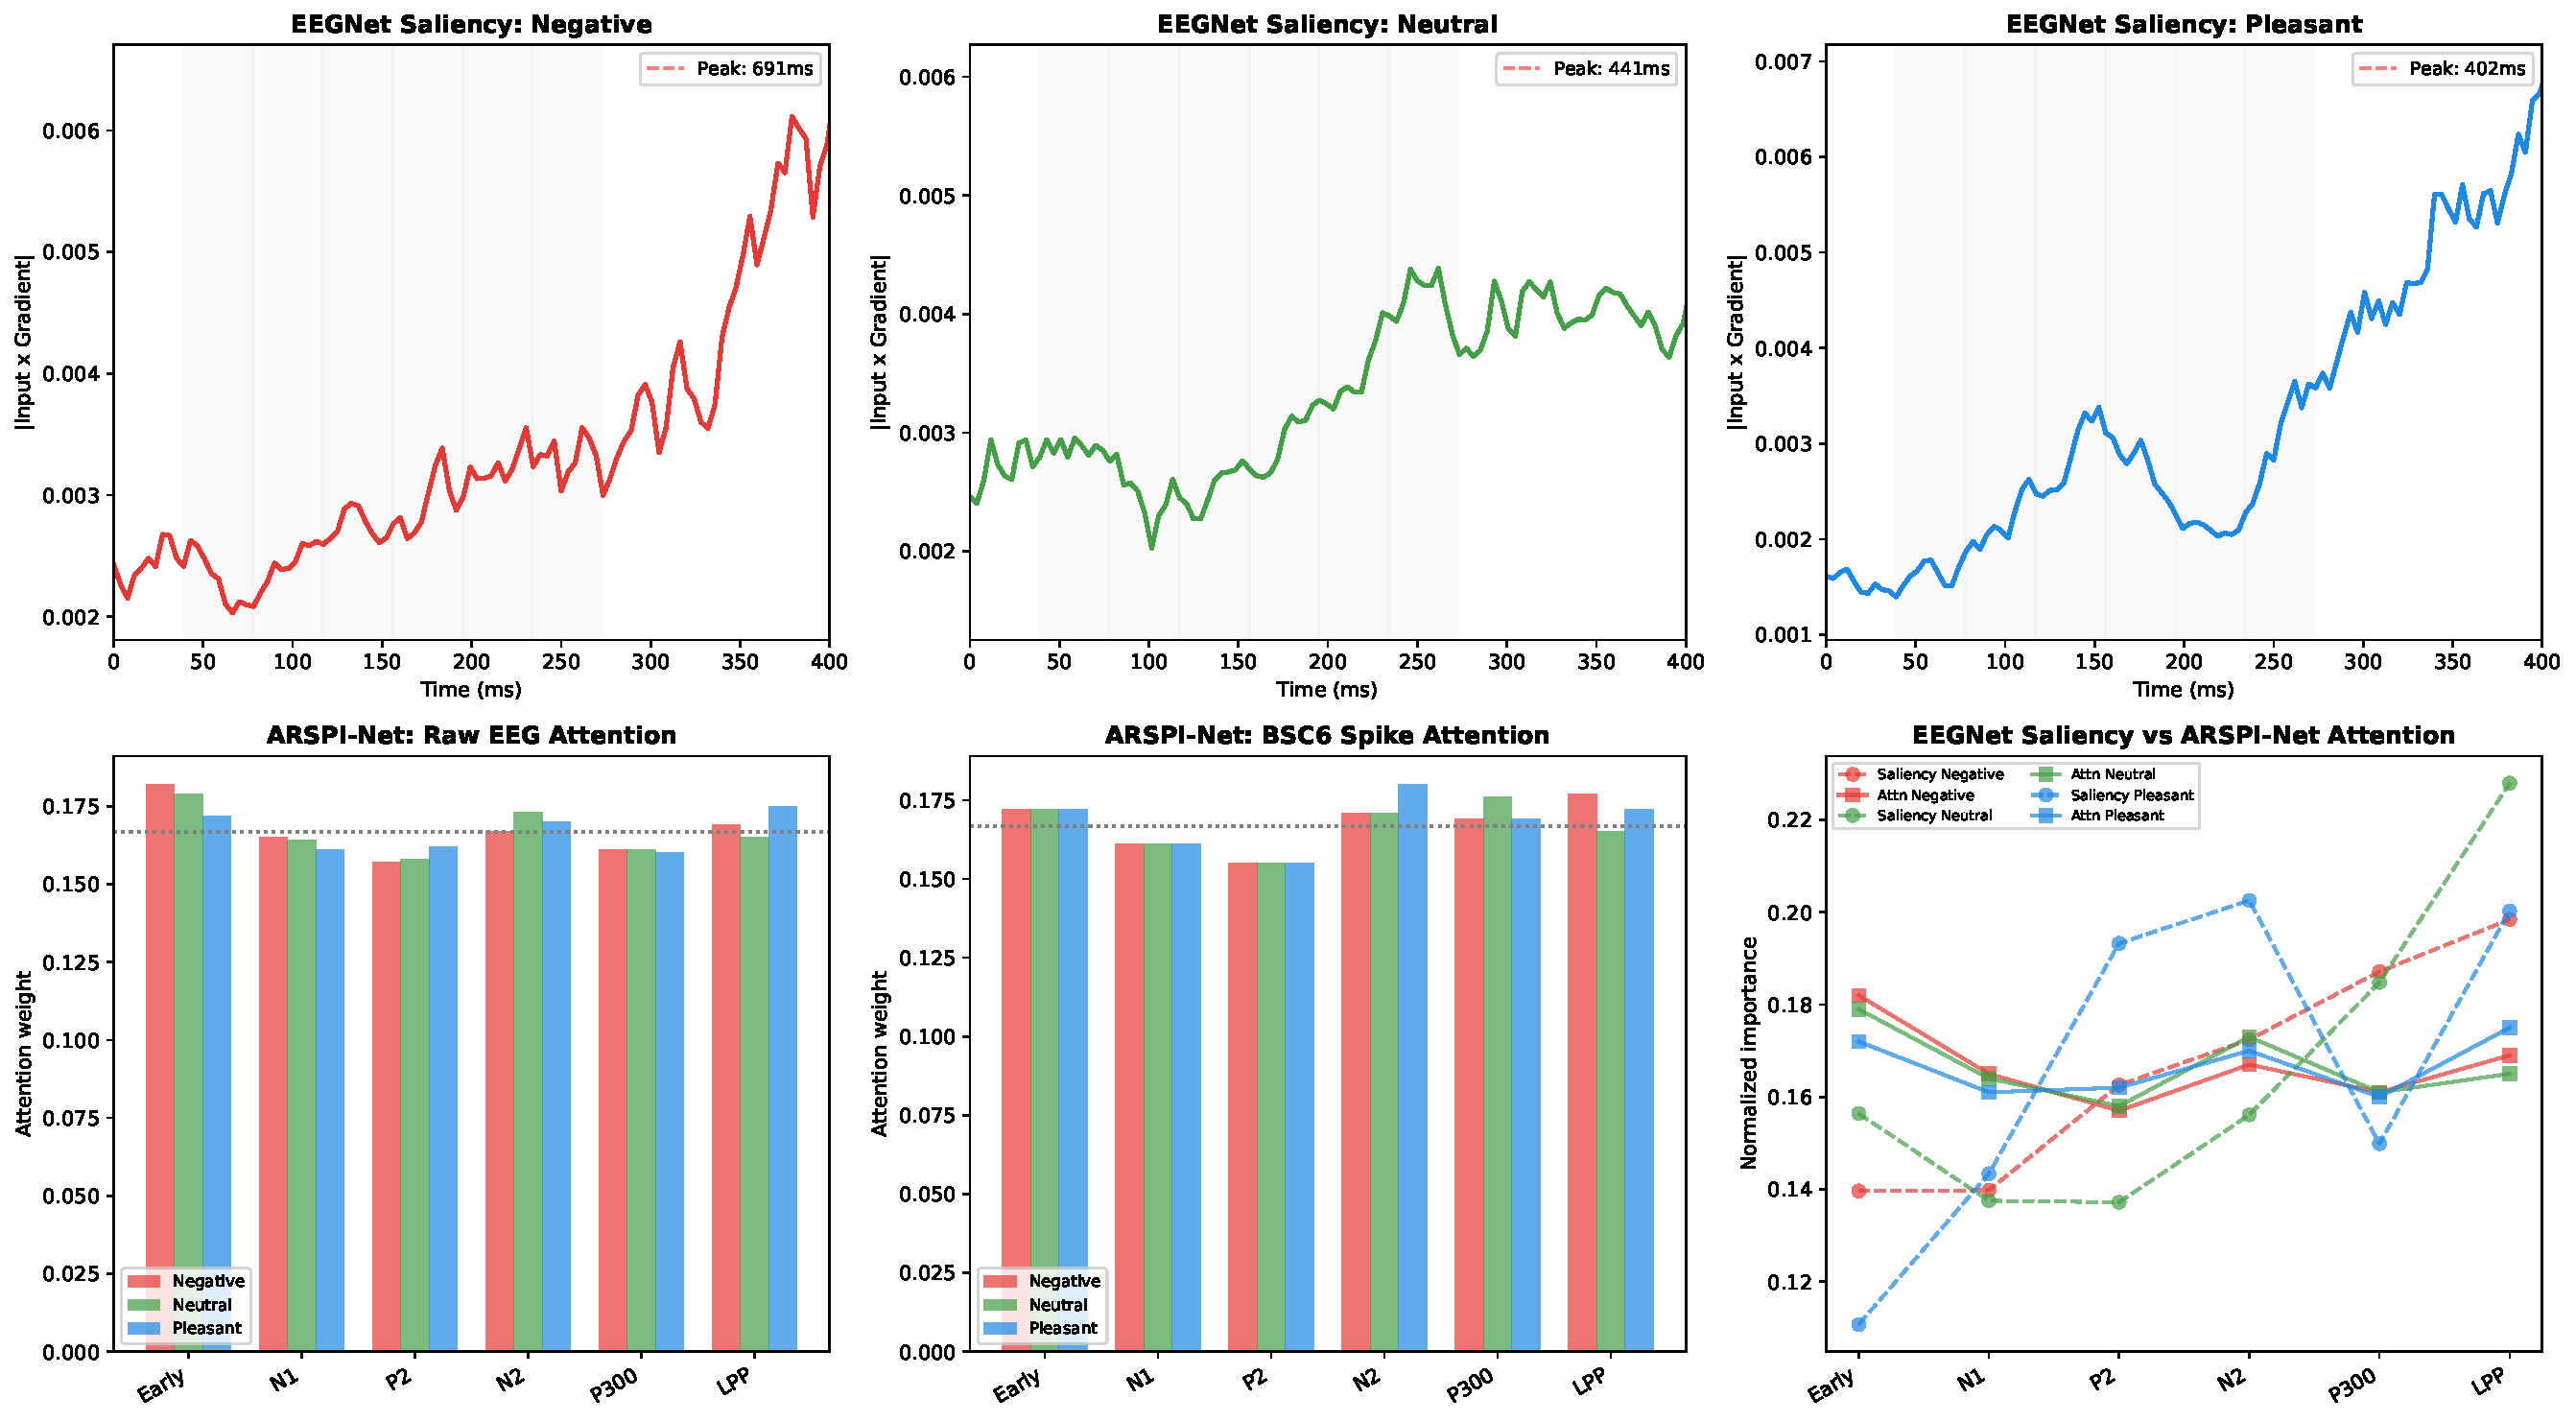
\includegraphics[width=\textwidth]{pictures/chGraphNeuralNetworks/fig_shap_comparison.pdf}
\caption[Temporal attribution summaries for EEGNet and ARSPI-Net.]{Temporal attribution summaries for EEGNet (input--gradient products, top row) and ARSPI-Net (learned attention weights, bottom left and center). EEGNet's unbinned maxima occur at $691$~ms (Negative), $441$~ms (Neutral), and $402$~ms (Pleasant). The bottom-right panel aligns both displays to the same six early intervals. The ARSPI-Net condition-profile permutation test gives $p=0.634$.}
\label{fig:shap_comparison}
\end{figure}

\paragraph{Interpretation.} Both quantities are model-dependent attribution summaries. The input--gradient product is post hoc, while ARSPI-Net attention is learned on predefined temporal bins. Mapping a weight to a bin improves traceability, but does not establish causal fidelity or exclude nuisance structure. Accuracy differences cannot be interpreted as the cost of interpretability because the model classes and training procedures differ. The two displays assign weight to different temporal regions under these fitted models.




\section{Connection to Dynamical Analysis}
\label{sec:ch5_bridge}

This chapter characterizes the archived embedding and graph-summary blocks. The feature-block analysis shows the largest emotion-label point estimates for embedding-containing models, while clinical-label estimates remain near chance and do not establish disorder detection. Chapter~\ref{chap:dynamics} describes reservoir-trajectory summaries, and Chapter~\ref{chap:synthesis} examines their descriptive association with graph summaries across channel indices.


\section{Chapter Summary}
\label{sec:ch5_summary}

This chapter reports analyses of $211$ participants ($633$ observations in the three-class data and $844$ in the four-class data). The post-defense audit changes the status of several results: PCA-dependent and incompatible-basis graph values are descriptive legacy estimates pending rerun with raw SHAPE data.

First, the archived variance decomposition assigns more variation to participants than conditions. Panel centering increases the displayed estimates across the tested representations, but it uses all three held-out observations for each subject and is not a prospective single-observation estimate.

Second, none of the tested propagation operators exceeds the non-propagated comparison in the archived sweep. This result is configuration- and cohort-specific.

Third, removing leading global-PCA components reduces the archived accuracy. The analysis does not prove that subject and condition effects occupy identical population subspaces.

Fourth, the exploratory clinical screen contains nominal SUD comparisons, but the strongest label-permutation check yields $p=0.073$, edge results do not survive FDR correction, and the nested-sample check is not an independent replication.

Fifth, the three- and four-class runs show different point-estimate rankings, but pipeline differences and global preprocessing confound the comparison; no regime transition or disorder hierarchy is established.

Sixth, embedding-containing models have the largest archived emotion-label point estimates in the feature-block comparison. A fold-safe rerun and nested comparison are needed before making an incremental-information claim.

Seventh, the clinical-label block estimates are mostly near chance, and post-hoc maxima do not establish layer-specific clinical sensitivity.

Finally, the baseline table records archived point estimates for several models. Differences in training protocols, global preprocessing, and the transductive panel-centering estimand prevent a definitive architecture ranking or a claim of intrinsic interpretability.

\newpage
\chapter{Dynamical Characterization of Reservoir Responses}
\label{chap:dynamics}

\section{Introduction and Motivation}

This chapter asks what can be learned by summarizing the reservoir trajectory rather than only its final embedding. The summaries are explicitly defined functions of a driven nonlinear system. They make intermediate computations inspectable, but they are not assumed to be physiological measurements or clinically meaningful variables.

The preceding chapters specify a fixed reservoir followed by channel-organized analysis. Here the reservoir trajectory is summarized with quantities that have stated definitions, units, or scales, and their within-cohort associations with input condition are described.

The analysis uses the selected reservoir operating point ($\beta = 0.05$, $M_{th}=0.5$, $N_{res}=256$), extracts seven summaries from all $633$ SHAPE observations, and screens variation by affective condition and clinical label. The summaries cover sparse activity, trajectory complexity, and response persistence. They make the reservoir response analyzable without implying clinical actionability.

All seven dynamical metrics have nominal Friedman $p < 0.05$ for the condition comparison, but this seven-test family was not multiplicity controlled. The mean effect-size magnitude in the two-member temporal-structure group ($\hat{H}_{\pi}$, $\tau_{AC}$) is $2.4\times$ that of the four-member amplitude-associated group. None of the $49$ channel-averaged metric--diagnosis screens has nominal $p<0.05$, and the clinical balanced-accuracy estimates are near chance. The later ``excitability--persistence'' label is therefore a descriptive name for an in-sample principal component, not a patient-level scale.

\section{Notation and Formal Definitions}
\label{sec:dynamics_notation}

The following definitions specify the reservoir state and the summaries used in this chapter.

\subsection{The LSM as a Driven Dynamical System}

The selected LSM reservoir has $N_{res}=256$ leaky integrate-and-fire neurons, fixed random input weights $\mathbf{W}^{in} \in \mathbb{R}^{N_{res} \times N_f}$, fixed random recurrent weights $\mathbf{W}^{rec} \in \mathbb{R}^{N_{res} \times N_{res}}$, membrane decay parameter $\beta=0.05$ (corresponding to $\tau_m \approx 20$ time steps), and firing threshold $M_{th}=0.5$. The reservoir receives one EEG channel as its input.

\paragraph{Definition 6.1 (Input Process).}
For a given subject $s$ and trial $j$, let $\mathbf{u}^{(j)}_s(t) \in \mathbb{R}^{N_f}$ denote the preprocessed EEG input vector at discrete time step $t \in \{1,\ldots,T\}$, where $T$ is the epoch length and $N_f$ is the number of input features per time step.

\paragraph{Definition 6.2 (Reservoir State).}
The retained post-update reservoir state at time $t$ is the membrane-potential vector
\begin{equation}
\mathbf{M}(t) = [M_1(t), M_2(t), \ldots, M_{N_{res}}(t)]^{\top} \in \mathbb{R}^{N_{res}}
\end{equation}
The implementation first computes the pre-reset value
\begin{equation}
\widetilde{M}_i[t] = (1-\beta)M_i[t-1](1-S_i[t-1]) + I_{tot,i}[t]
\end{equation}
where $S_i[t-1] \in \{0,1\}$ is the spike indicator at the previous step and
\begin{equation}
I_{tot,i}[t] = \sum_{j=1}^{N_f} W^{in}_{ij}u_j(t) + \sum_{\ell=1}^{N_{res}} W^{rec}_{i\ell}S_{\ell}[t-1].
\end{equation}
A spike is emitted when $\widetilde{M}_i[t] \ge M_{th}$:
\begin{equation}
S_i[t] = \Theta(\widetilde{M}_i[t]-M_{th}),
\end{equation}
and the retained state is
\begin{equation}
M_i[t]=\max\!\left(\widetilde{M}_i[t]-S_i[t]M_{th},\,0\right),
\end{equation}
where $\Theta(\cdot)$ is the Heaviside step function. Thus a unit that spikes has its threshold subtracted on the current step and its retained contribution cleared in the next-step decay term.

\paragraph{Definition 6.3 (Spike Train Matrix).}
For a given trial, the complete spike output of the reservoir is the binary matrix
\begin{equation}
\mathbf{S} \in \{0,1\}^{N_{res}\times T}, \qquad S_{i,t}=S_i[t].
\end{equation}

\paragraph{Definition 6.4 (Global Firing Rate).}
The instantaneous population firing rate at time $t$ is
\begin{equation}
r(t)=\frac{1}{N_{res}}\sum_{i=1}^{N_{res}} S_i[t].
\end{equation}

\paragraph{Definition 6.5 (Driven System Emphasis).}
For a fixed reservoir instantiation (fixed $\mathbf{W}^{in}$ and $\mathbf{W}^{rec}$), the reservoir state trajectory $\mathbf{M}(1),\mathbf{M}(2),\ldots,\mathbf{M}(T)$ is a deterministic function of the input sequence $\mathbf{u}(1),\mathbf{u}(2),\ldots,\mathbf{u}(T)$. We denote the mapping from input sequence to state trajectory as
\begin{equation}
\mathcal{R}: \mathbb{R}^{N_f \times T} \rightarrow \mathbb{R}^{N_{res} \times T}.
\end{equation}
All dynamical metrics extracted in this chapter are properties of $\mathcal{R}(\mathbf{u})$, the driven trajectory, not of $\mathcal{R}$ in isolation.

\section{Metric I: Sparse Coding Efficiency \texorpdfstring{($\Phi$)}{(Phi)}}
\label{sec:dynamics_phi}

\subsection{Theoretical Foundation}

The efficient-coding literature motivates comparing information retained by a representation with the operations needed to compute it \cite{barlow_possible_1961,olshausen_emergence_1996}. In this software implementation, spike counts can support an operation-count estimate. They cannot establish metabolic cost, physical energy use, or pathological inefficiency. The dissertation therefore treats this metric as engineering bookkeeping rather than a biological hypothesis.

\subsection{Formal Metric Definition}

\paragraph{Definition 6.6 (Total Synaptic Operations).}
For a single trial with spike train matrix $\mathbf{S}$, the total synaptic operations count is
\begin{equation}
\mathrm{SynOps} = \sum_{t=1}^{T} \left[ \sum_{i=1}^{N_{res}} S_i[t] \cdot \left(\mathrm{fan\mbox{-}out}^{rec}_i + \mathrm{fan\mbox{-}out}^{read}_i\right) \right]
\end{equation}
where $\mathrm{fan\mbox{-}out}^{rec}_i$ is the number of nonzero outgoing recurrent connections from neuron $i$ and $\mathrm{fan\mbox{-}out}^{read}_i$ is the number of readout connections. For a fully connected readout to $N_{out}$ output neurons,
\begin{equation}
\mathrm{SynOps} = \sum_{t=1}^{T} \sum_{i=1}^{N_{res}} S_i[t] \cdot (d_i^{rec}+N_{out})
\end{equation}
where $d_i^{rec}$ is the recurrent out-degree of neuron $i$.

Under sparse random connectivity with connection probability $p_c$, the expected recurrent fan-out per neuron is $p_cN_{res}$, yielding the simplified estimator
\begin{equation}
\mathrm{SynOps} \approx N_{total\_spikes}\cdot (p_cN_{res}+N_{out})
\end{equation}
where $N_{total\_spikes}=\sum_{i,t} S_{i,t}$ is the total spike count over the epoch.

\paragraph{Definition 6.7 (Hardware-Model Energy Estimate).}
If a specified hardware platform assigns energy $E_{syn}$ to each synaptic operation, a model-based trial estimate would be
\begin{equation}
E_{trial}=\mathrm{SynOps}\cdot E_{syn}. 
\end{equation}

\paragraph{Definition 6.8 (Decoded Information Summary).}
Let $f(\mathbf{S})$ denote a feature vector extracted from the spike train and let $\hat{y}$ be an out-of-fold prediction produced from that vector. The mutual information between the observed label and the decoded label can be computed from the out-of-fold confusion matrix:
\begin{equation}
\hat{I}(y;\hat{y})=\sum_{k=1}^{K}\sum_{\hat{k}=1}^{K} p(y=k,\hat{y}=\hat{k})\log_2\!\left(\frac{p(y=k,\hat{y}=\hat{k})}{p(y=k)\,p(\hat{y}=\hat{k})}\right).
\end{equation}
Because $y\rightarrow\mathbf{S}\rightarrow f(\mathbf{S})\rightarrow\hat{y}$ is a processing chain, $I(y;\mathbf{S})\geq I(y;\hat{y})$ by the data processing inequality. This is a dataset-level decoder summary, not a per-trial estimate of the information in the spike train. It must be computed from genuinely out-of-fold predictions; accuracy alone is insufficient to determine it.

\paragraph{Definition 6.9 (Operation-Normalized Decoder Summary).}
When fold-safe out-of-fold predictions are available, an operation-normalized descriptive summary may be reported as
\begin{equation}
\Phi_{dataset} = \frac{\hat{I}(y;\hat{y})}{\overline{\mathrm{SynOps}}} \qquad \left[\frac{\mathrm{bits}}{\mathrm{mean\ trial\ synaptic\ operation}}\right]
\end{equation}
where $\overline{\mathrm{SynOps}}$ is the mean estimated operation count per trial. This ratio is one dataset-level descriptive number. It does not define a trial-level or condition-level information efficiency distribution. A physical energy quantity would additionally require hardware-specific measurements; multiplying by a literature energy-per-operation constant provides only a hardware-model estimate.
For completeness, a hardware-model normalization would be
\begin{equation}
\Phi_E = \frac{\hat{I}(y;\hat{y})}{\overline{E}_{trial}} \qquad \left[\frac{\mathrm{bits}}{\mathrm{Joule}}\right],
\end{equation}
but it is not evaluated in this dissertation because no neuromorphic hardware was profiled.

\subsection{Auxiliary Metrics}

\paragraph{Definition 6.10 (Population Sparsity).}
The lifetime sparsity of the population response is measured by the Treves--Rolls sparsity index
\begin{equation}
a = \frac{\left(\frac{1}{N_{res}}\sum_{i=1}^{N_{res}} \bar{r}_i\right)^2}{\frac{1}{N_{res}}\sum_{i=1}^{N_{res}} \bar{r}_i^2}
\end{equation}
where $\bar{r}_i=(1/T)\sum_t S_i[t]$ is the mean firing rate of neuron $i$ over the epoch.

\paragraph{Definition 6.11 (Temporal Sparsity).}
The fraction of time steps in which the population is quiescent is
\begin{equation}
a_{temp}=\frac{1}{T}\sum_{t=1}^{T} \mathbb{1}[r(t)<\epsilon].
\end{equation}
In implementation, $\epsilon$ may be chosen as $1/N_{res}$, corresponding to at most one spike per time step.

\subsection{Scope of the Efficiency Summary}
Because $\Phi_{dataset}$ is defined from a single out-of-fold confusion matrix, it is not a participant-level variable and cannot be compared between individual HC and MDD observations. The archived analysis treated a fixed decoded-information numerator divided by each trial's spike count as though it were trial-level information efficiency. That construction is not used here. EXP-6.5 therefore reports only the observed operation-count stability; no clinical information-efficiency hypothesis is tested.

\section{Metric II: Driven Trajectory Complexity \texorpdfstring{($\Lambda$)}{(Lambda)}}
\label{sec:dynamics_lambda}

\subsection{Theoretical Foundation}

The edge-of-chaos hypothesis motivates studying contraction and expansion in recurrent systems \cite{langton_computation_1990,bertschinger_real-time_2004}. For a driven reservoir, the relevant quantity is the separation rate of nearby reservoir trajectories under the \emph{same} input, not the autonomous Lyapunov spectrum. Any clinical direction proposed below is exploratory; no theorem links diagnostic status to the complexity of this fixed reservoir's response.

\subsection{Formal Metric Definitions}

\subsubsection{The Largest Lyapunov Exponent of the Driven Reservoir}

\paragraph{Definition 6.12 (Driven Lyapunov Exponent).}
Consider the driven reservoir as a discrete-time dynamical system
\begin{equation}
\mathbf{M}[t+1]=\mathbf{F}(\mathbf{M}[t],\mathbf{u}[t]).
\end{equation}
The driven Lyapunov exponent quantifies the average exponential rate of separation of infinitesimally close trajectories under the same input drive. Let $\delta \mathbf{M}[0]$ be a small perturbation to the initial state and let the perturbed trajectory evolve as
\begin{equation}
\mathbf{M}'[t+1]=\mathbf{F}(\mathbf{M}'[t],\mathbf{u}[t]).
\end{equation}
Then
\begin{equation}
\lambda_1 = \lim_{T\to\infty}\frac{1}{T}\sum_{t=0}^{T-1}\ln\frac{\lVert \delta \mathbf{M}[t+1]\rVert}{\lVert \delta \mathbf{M}[t]\rVert}
\end{equation}
where $\delta \mathbf{M}[t]=\mathbf{M}'[t]-\mathbf{M}[t]$.

The threshold-and-reset operation in leaky integrate-and-fire dynamics introduces a discontinuity, so the tangent-space calculation must account for spike events explicitly. Event-based Lyapunov calculations for LIF networks have been developed in prior work on spiking-network stability and can be used to motivate the projection treatment at threshold crossings \cite{monteforte_dynamic_2012}. For finite EEG epochs, the practical estimate used in this chapter follows the standard renormalization strategy associated with Benettin-style Lyapunov computation \cite{benettin_lyapunov_1980}:
\begin{enumerate}
    \item Initialize the reservoir at state $\mathbf{M}[0]$ and a nearby state $\mathbf{M}'[0]=\mathbf{M}[0]+\delta_0\hat{\mathbf{e}}$, where $\hat{\mathbf{e}}$ is a random unit vector and $\delta_0=10^{-8}$.
    \item Evolve both trajectories under the same input $\mathbf{u}(t)$ for $T_{renorm}$ steps.
    \item Compute the stretching factor $\gamma_k = \lVert \mathbf{M}'[kT_{renorm}] - \mathbf{M}[kT_{renorm}] \rVert/\delta_0$.
    \item Renormalize the perturbed trajectory along the instantaneous separation direction.
    \item Repeat for $K$ renormalization intervals and estimate
    \begin{equation}
    \hat{\lambda}_1 = \frac{1}{KT_{renorm}}\sum_{k=1}^{K}\ln(\gamma_k).
    \end{equation}
\end{enumerate}

\subsubsection{Lempel--Ziv Complexity ($C_{LZ}$)}

\paragraph{Definition 6.13 (Lempel--Ziv Complexity of Reservoir Spike Output).}
For a single neuron $i$, let $s_i=S_i[1]S_i[2]\cdots S_i[T]$ be the binary spike sequence. The normalized Lempel--Ziv complexity is
\begin{equation}
C_{LZ,i}=\frac{c(s_i)}{T/\log_2(T)}
\end{equation}
where $c(s_i)$ is the number of distinct substrings generated by the LZ76 parsing procedure. The population-level complexity is
\begin{equation}
C_{LZ}=\frac{1}{N_{res}}\sum_{i=1}^{N_{res}} C_{LZ,i}.
\end{equation}

\subsubsection{Permutation Entropy ($H_{\pi}$)}

\paragraph{Definition 6.14 (Permutation Entropy of Membrane Potential Trajectory).}
As a complementary complexity measure operating on the continuous-valued membrane potentials rather than the binary spike trains, define the global mean membrane potential
\begin{equation}
\bar{M}(t)=\frac{1}{N_{res}}\sum_{i=1}^{N_{res}} M_i[t].
\end{equation}
For embedding dimension $d$ and delay $\tau$, ordinal patterns are constructed from $[\bar{M}(t),\bar{M}(t+\tau),\ldots,\bar{M}(t+(d-1)\tau)]$. The permutation entropy is then
\begin{equation}
H_{\pi}=-\sum_{\pi\in S_d} p(\pi)\log_2 p(\pi)
\end{equation}
with normalized form
\begin{equation}
\hat{H}_{\pi}=\frac{H_{\pi}}{\log_2(d!)}.
\end{equation}
Permutation entropy was introduced by Bandt and Pompe as a natural complexity measure for time series \cite{bandt_permutation_2002}.

\subsection{Phase-Space Visualization}

\paragraph{Definition 6.15 (Reconstructed Phase Portrait).}
For visualization of a finite driven trajectory, let $\mathbf{M} \in \mathbb{R}^{N_{res}\times T}$ be the membrane-potential matrix for a given observation. Compute the PCA projection
\begin{equation}
\mathbf{z}(t)=\mathbf{W}_{PC}^{\top}(\mathbf{M}(t)-\bar{\mathbf{M}}) \in \mathbb{R}^{2}
\end{equation}
where $\mathbf{W}_{PC}=[\mathbf{w}_1,\mathbf{w}_2]$ contains the first two principal-component directions and $\bar{\mathbf{M}}$ is the temporal mean.

\subsection{Hypothesis H2}
An exploratory directional hypothesis is that reservoir trajectories driven by EEG from the complete-case control group will have larger complexity summaries than trajectories from participants with MDD:
\begin{equation}
\mathbb{E}[\Lambda\mid \mathrm{HC}] > \mathbb{E}[\Lambda\mid \mathrm{MDD}]
\end{equation}
where $\Lambda \in \{\lambda_1,C_{LZ},\hat{H}_{\pi}\}$. This hypothesis is tested in Section~\ref{sec:ch6_results}, EXP-6.6.

\section{Metric III: Relaxation Time Constant \texorpdfstring{($T$)}{(T)}}
\label{sec:dynamics_tau}

\subsection{Theoretical Foundation}

Critical slowing down describes slower recovery near some dynamical transitions \cite{scheffer_early-warning_2009}, and elevated temporal autocorrelation has been proposed as an early-warning signal in affective time series \cite{vandeleemput_critical_2014,wichers_critical_2016}. The present quantity is narrower: it summarizes decay in the fixed reservoir's population response over an observed epoch. It is not a cortical recovery or tipping-point estimate.

\subsection{Formal Metric Definitions}

\subsubsection{Exponential Relaxation Time ($\tau_{relax}$)}

\paragraph{Definition 6.16 (Relaxation Time Constant).}
Consider the global firing rate $r(t)$ during the post-stimulus window $[t_{onset},t_{end}]$. Define
\begin{equation}
r_{peak}=\max_{t\in[t_{onset},t_{end}]} r(t), \qquad t_{peak}=\arg\max_{t\in[t_{onset},t_{end}]} r(t).
\end{equation}
The relaxation phase is $[t_{peak},t_{end}]$. Model the decay of the firing-rate envelope as
\begin{equation}
r(t) \approx r_{\infty} + (r_{peak}-r_{\infty})\exp\left(-\frac{t-t_{peak}}{\tau_{relax}}\right), \qquad t\ge t_{peak}
\end{equation}
where $r_{\infty}$ is estimated from the final portion of the epoch.

\subsubsection{Autocorrelation Decay Rate}

\paragraph{Definition 6.17 (Lag-$k$ Autocorrelation of Population Firing Rate).}
The normalized autocorrelation function of the global firing rate is
\begin{equation}
\rho(k)=\frac{\sum_{t=1}^{T-k}(r(t)-\bar{r})(r(t+k)-\bar{r})}{\sum_{t=1}^{T}(r(t)-\bar{r})^2}
\end{equation}
where $\bar{r}=(1/T)\sum_t r(t)$.

\paragraph{Definition 6.18 (Autocorrelation Decay Constant).}
Define
\begin{equation}
\tau_{AC}=\min\{k\ge 1: \rho(k)\le e^{-1}\}
\end{equation}
or estimate $\tau_{AC}$ by fitting an exponential decay model to $\rho(k)$.

\subsubsection{Attractor Depth via Return-to-Baseline Time}

\paragraph{Definition 6.19 (Return-to-Baseline Time).}
Let the baseline firing rate be
\begin{equation}
r_{baseline}=\frac{1}{|[1,t_{onset}]|}\sum_{t=1}^{t_{onset}} r(t).
\end{equation}
The return-to-baseline time is
\begin{equation}
T_{RTB}=\min\left\{t>t_{peak}: r(t')\le r_{baseline}+\alpha(r_{peak}-r_{baseline})\ \forall\ t'\in[t,t+\Delta]\right\}-t_{peak}
\end{equation}
where $\alpha\in(0,1)$ is a threshold fraction and $\Delta$ is a sustain window.

\subsection{Linearized Decay Analogy}

For an autonomous system linearized near a stable operating point, the eigenvalue of largest magnitude inside the unit disk determines the slowest decay mode. If that eigenvalue is $\mu_{max}$, then
\begin{equation}
\tau_{relax}^{(slow)} = -\frac{1}{\ln|\mu_{max}|}.
\end{equation}
As $|\mu_{max}|\rightarrow 1^{-}$, this linearized time constant increases. The driven, thresholded reservoir analyzed here does not meet this simple model exactly, so the equation is contextual rather than an identification of an energy landscape or critical point.

\subsection{Hypothesis H3}
As an exploratory engineering hypothesis, EEG from participants with MDD may place the fixed reservoir in a regime with a longer measured relaxation time than EEG from healthy controls:
\begin{equation}
\mathbb{E}[\tau_{relax}\mid \mathrm{MDD}] > \mathbb{E}[\tau_{relax}\mid \mathrm{HC}].
\end{equation}
This hypothesis is tested in Section~\ref{sec:ch6_results}, EXP-6.6. The test concerns the response of the fixed reservoir to the observed EEG; it is not a test of cortical criticality and does not estimate a cortical relaxation time.

\section{Validity and Scope of Reservoir-Derived Measures}
\label{sec:dynamics_fidelity}

This section states the conditions under which a quantity extracted from the driven reservoir can be interpreted. The analysis distinguishes three objects: the latent cortical process, the scalp EEG observation, and the response of the fixed reservoir to that observation. The metrics in this chapter describe the third object. They are not estimators of latent cortical invariants unless a separate validation establishes such a relationship.

\subsection{Fixed-Transformation Perspective}

A fixed transformation can be characterized by how it responds to controlled and observed inputs. The reservoir is treated in that limited sense: as a specified nonlinear operator whose internal state is available for inspection. It was not calibrated as a scientific instrument. The metrics are functionals of the \emph{driven reservoir response}, not latent cortical invariants.

In particular, the reservoir relaxation time is not the relaxation time of the cortex. It is a response functional of a specified nonlinear filter. Reliability across repeated recordings, reservoir initializations, and preprocessing choices would be required before that functional could support an individual-level interpretation.

\subsection{Formal Signal-Chain Setup}

Let $\theta \in \Theta$ denote a latent clinical or affective state parameter, let $\mathbf{X}(t;\theta)$ denote the latent cortical source process, and let the observed EEG be modeled as
\begin{equation}
\mathbf{u}(t;\theta)=\mathbf{L}\mathbf{X}(t;\theta)+\boldsymbol{\eta}(t)
\end{equation}
where $\mathbf{L}$ is a lead-field or mixing operator and $\boldsymbol{\eta}(t)$ denotes sensor noise. Let $\mathbf{M}(t;\theta,\omega)$ denote the reservoir membrane-potential trajectory produced by input $\mathbf{u}(t;\theta)$ under reservoir instantiation $\omega=(\mathbf{W}^{in},\mathbf{W}^{rec})$, and let $\Psi[\mathbf{M}]$ denote a dynamical functional such as $\Phi$, $\lambda_1$, or $\tau_{relax}$.

The full processing chain can then be written as
\begin{equation}
\theta \rightarrow \mathbf{X}(t;\theta) \rightarrow \mathbf{u}(t;\theta) \rightarrow \mathbf{M}(t;\theta,\omega) \rightarrow \Psi(\theta,\omega).
\end{equation}
The three core validity questions are then:
\begin{enumerate}
    \item Is $\mathbf{M}(t;\theta,\omega)$ effectively determined by $\mathbf{u}(t;\theta)$ rather than by its initial condition?
    \item Does the reservoir retain sufficient information about the clinically relevant structure in $\mathbf{u}(t;\theta)$?
    \item Does the chosen functional $\Psi$ preserve the ordering or magnitude of the input property of interest?
\end{enumerate}
These questions separate state reproducibility, retained task information, and external validity. Satisfying one does not imply the others.

\subsection{Input Determinism: Echo State Property and Generalized Synchronization}

To interpret the reservoir as an input-determined filter, its dependence on the initial state must decay for the input class under study. The echo state property formalizes such loss of initial-condition dependence. Simple spectral-radius heuristics are insufficient even for smooth tanh reservoirs, and the property belongs to the driven system rather than to the recurrent matrix alone \cite{yildiz_re-visiting_2012}. The piecewise-smooth LIF update requires at least the same caution.

Formally, the reservoir satisfies the ESP with respect to an input class $\mathcal{U}$ if, for every bounded input sequence $\mathbf{u}\in\mathcal{U}$ and every pair of initial conditions $\mathbf{M}_0,\mathbf{M}_0'$,
\begin{equation}
\lim_{t\rightarrow\infty}\left\|\mathbf{M}(t;\mathbf{M}_0,\mathbf{u})-\mathbf{M}(t;\mathbf{M}_0',\mathbf{u})\right\|=0.
\end{equation}
A fully rigorous sufficient condition for the particular discretized LIF reservoir used here is nontrivial because the threshold-and-reset mechanism breaks global smoothness. For that reason, the strongest defensible statement is not a universal theorem for all bounded inputs, but an input-class statement: if the driven reservoir has negative conditional Lyapunov exponent over the input family of interest, then it contracts initial-condition differences and behaves as an input-determined filter. That logic is entirely consistent with generalized synchronization theory, which states that a driven system can converge onto a synchronization manifold that is a deterministic function of the input history \cite{rulkov_generalized_1995,yildiz_re-visiting_2012}.

Accordingly, a negative driven conditional Lyapunov estimate is used here as evidence of contraction for the tested input family:
\begin{equation}
\lambda_1^{(driven)} < 0 \quad \Longrightarrow \quad \mathbf{M}(t) \approx \psi(\mathbf{u}(t),\mathbf{u}(t-1),\ldots)
\end{equation}
after transient decay, for the specific operating regime under study. This empirical criterion does not prove a global echo-state property for all bounded inputs and does not by itself prove separation between stimulus classes.

\subsection{Fading Memory and Effective Memory Horizon}

Once the state is a function of the input history, one still needs a practical bound on how much history matters. Reservoir systems with the fading-memory property weight remote lags less strongly than recent lags. An effective memory horizon $T_{mem}$ can therefore be defined operationally as the lag beyond which a controlled perturbation has negligible measured effect. The heuristic $T_{mem}\approx -1/\lambda_1$ may be useful near a uniformly contracting linearization, but it is not an identity for a thresholded, input-driven reservoir and is not used as a measured cortical timescale.

\subsection{Information-Theoretic Bounds}

The processing chain $\theta \rightarrow \mathbf{u} \rightarrow \mathbf{M} \rightarrow \Psi$ is a Markov chain. Therefore the data processing inequality implies
\begin{equation}
I(\theta;\Psi)\leq I(\theta;\mathbf{M})\leq I(\theta;\mathbf{u}),
\end{equation}
so neither the reservoir nor the downstream functional can create new information about the latent state that was not already present in the EEG input \cite{cover_elements_2006}. This bound is a necessary guardrail on the interpretation of Chapter 4 results. When the reservoir increases the Fisher Discriminant Ratio or improves downstream classification accuracy, the correct reading is that it improves \emph{representation geometry for the chosen decoder}, not that it increases mutual information in violation of DPI.

Any reservoir-derived metric must therefore be evaluated relative to information already present in the observed EEG, not relative to an unobserved cortical state.

\subsection{Takens-Type Embedding and Dynamical Sufficiency}

Takens' original theorem concerns smooth, deterministic, autonomous dynamical systems observed through generic scalar functions; under those assumptions, a delay embedding can reconstruct the attractor up to a diffeomorphism \cite{takens_detecting_1981}. Those assumptions do \emph{not} hold literally for noisy, volume-conducted EEG, and they certainly do not hold automatically for a discontinuous spiking reservoir. Any appeal to Takens in this dissertation must therefore be treated as an analogy supported by more recent reservoir-embedding results, not as a direct theorem about the SHAPE EEG itself.

Recent ESN theory is relevant but does not close this gap. Hart, Hook, and Dawes show that a suitable ESN trained on observations of an invertible dynamical system can induce an echo-state map that is generically an embedding with positive probability \cite{hart_embedding_2020}. Grigoryeva and Ortega establish fading-memory and approximation properties for reservoir systems under bounded inputs \cite{grigoryeva_echo_2018}. Those assumptions do not prove that the LIF reservoir used here is a diffeomorphic embedding of latent cortical dynamics. The results motivate a representation hypothesis; they are not presented as a theorem about SHAPE EEG.

\subsection{Metric-Specific Validity and Monotonicity}

The most difficult issue is not state reconstruction; it is whether a chosen functional of the reservoir trajectory preserves the ordering of the corresponding input property.

\paragraph{Complexity metrics.}
For symbolic measures such as Lempel--Ziv complexity and permutation entropy, no general monotonic mapping from input complexity to reservoir-output complexity is assumed. A nonlinear filter can increase or decrease either measure. Direct comparison with input-domain measures and controlled surrogates is therefore necessary \cite{lempel_complexity_1976,bandt_permutation_2002,zunino_permutation_2017,little_permutation_2016}.

\paragraph{Driven Lyapunov exponent.}
The driven Lyapunov exponent is a joint property of the input--reservoir system, not an estimator of the cortical Lyapunov spectrum. It depends on the reservoir Jacobian along the driven trajectory and on how the input positions neurons relative to threshold. It is therefore reported only as a reservoir-stability descriptor.

\paragraph{Relaxation-time metrics.}
During a locally linear decay phase, the population-rate time constant can depend on both intrinsic reservoir contraction and the autocorrelation structure of the input. It is therefore an input-mediated effective reservoir time constant. Its physiological meaning is not established here.

\subsection{Empirical Validation Requirements}

The theoretical considerations above are not substitutes for empirical validation. A complete validation would include:
\begin{enumerate}
    \item \textbf{Echo-state verification:} initialize the same reservoir/input pair from widely separated initial conditions and verify exponential convergence of the state difference.
    \item \textbf{Cross-initialization reliability:} compute ICC$(3,1)$ for each dynamical metric across multiple reservoir initializations and require at least good reliability.
    \item \textbf{Surrogate testing:} compare real-input metrics against phase-randomized or otherwise structure-destroyed surrogates. This must be interpreted carefully because IAAFT-type surrogates can themselves exhibit residual Fourier-phase issues if used incautiously \cite{rath_revisiting_2012}.
    \item \textbf{Direct raw-EEG correlation:} correlate reservoir metrics with directly measured EEG complexity or autocorrelation statistics to demonstrate grounding in the input process.
    \item \textbf{Permutation-based group inference:} use label-permutation tests to avoid overreliance on fragile parametric assumptions in small clinical cohorts.
\end{enumerate}

\subsection{Interpretive Boundary}

The driven reservoir must forget initial conditions over the tested input family; separability claims must be phrased as changes in decoder-accessible geometry rather than creation of information; and each proposed descriptor requires reliability, surrogate, and input-domain validation. The experiments below satisfy only part of that program. The resulting quantities are therefore treated as descriptive engineering measures of the reservoir response, not as biomarkers or direct physiological measurements.

\section{Experimental Protocol}
\label{sec:dynamics_protocol}

All experiments use the $211$-subject, three-class SHAPE dataset and preprocessing pipeline established in Chapter~\ref{chap:arspi_net}. For each of $633$ observations ($211$ subjects $\times$ $3$ conditions), $34$ EEG channels are individually processed through the fixed reservoir ($N_{res} = 256$, $\beta = 0.05$, $M_{th}=0.5$), producing $21{,}522$ total reservoir runs. The seven primary summaries are total spikes, mean firing rate, rate entropy, rate variance, temporal sparsity, permutation entropy, and autocorrelation decay. Four auxiliary summaries are also retained for sensitivity analyses. Theta-band ($4$--$8$ Hz) phase-concentration matrices are computed from the full-resolution $1{,}024$~Hz EEG for Chapter~\ref{chap:synthesis}. Statistical analysis uses within-subject paired comparisons for condition effects and between-group comparisons for clinical effects. Unless a correction is explicitly stated, the reported $p$ values are exploratory nominal values rather than family-wise confirmatory tests. Raw observations are presented in Appendix~\ref{app:ch6_figs}.


\section{Experimental Results}
\label{sec:ch6_results}

\subsection{EXP-6.1: Exploratory Condition Associations Across Seven Metrics}

All seven primary metrics have nominal Friedman $p<0.05$ (Figure~\ref{fig:ch6_condition_effects}). Negative and Pleasant have similar profiles, while Neutral is the largest contrast. The archived pairwise tests report nominal differences for Negative--Neutral and Neutral--Pleasant across all seven metrics and no nominal Negative--Pleasant difference. The largest standardized contrast is observed for $\tau_{AC}$: Negative ($5.65$) $>$ Pleasant ($5.50$) $>$ Neutral ($4.92$; $d_z=+0.35$ for Negative--Neutral). Because the seven omnibus tests and their post-hoc contrasts form a multiple-testing family, these results are treated as exploratory until reproduced under a prespecified correction.

\begin{figure}[H]
    \centering
    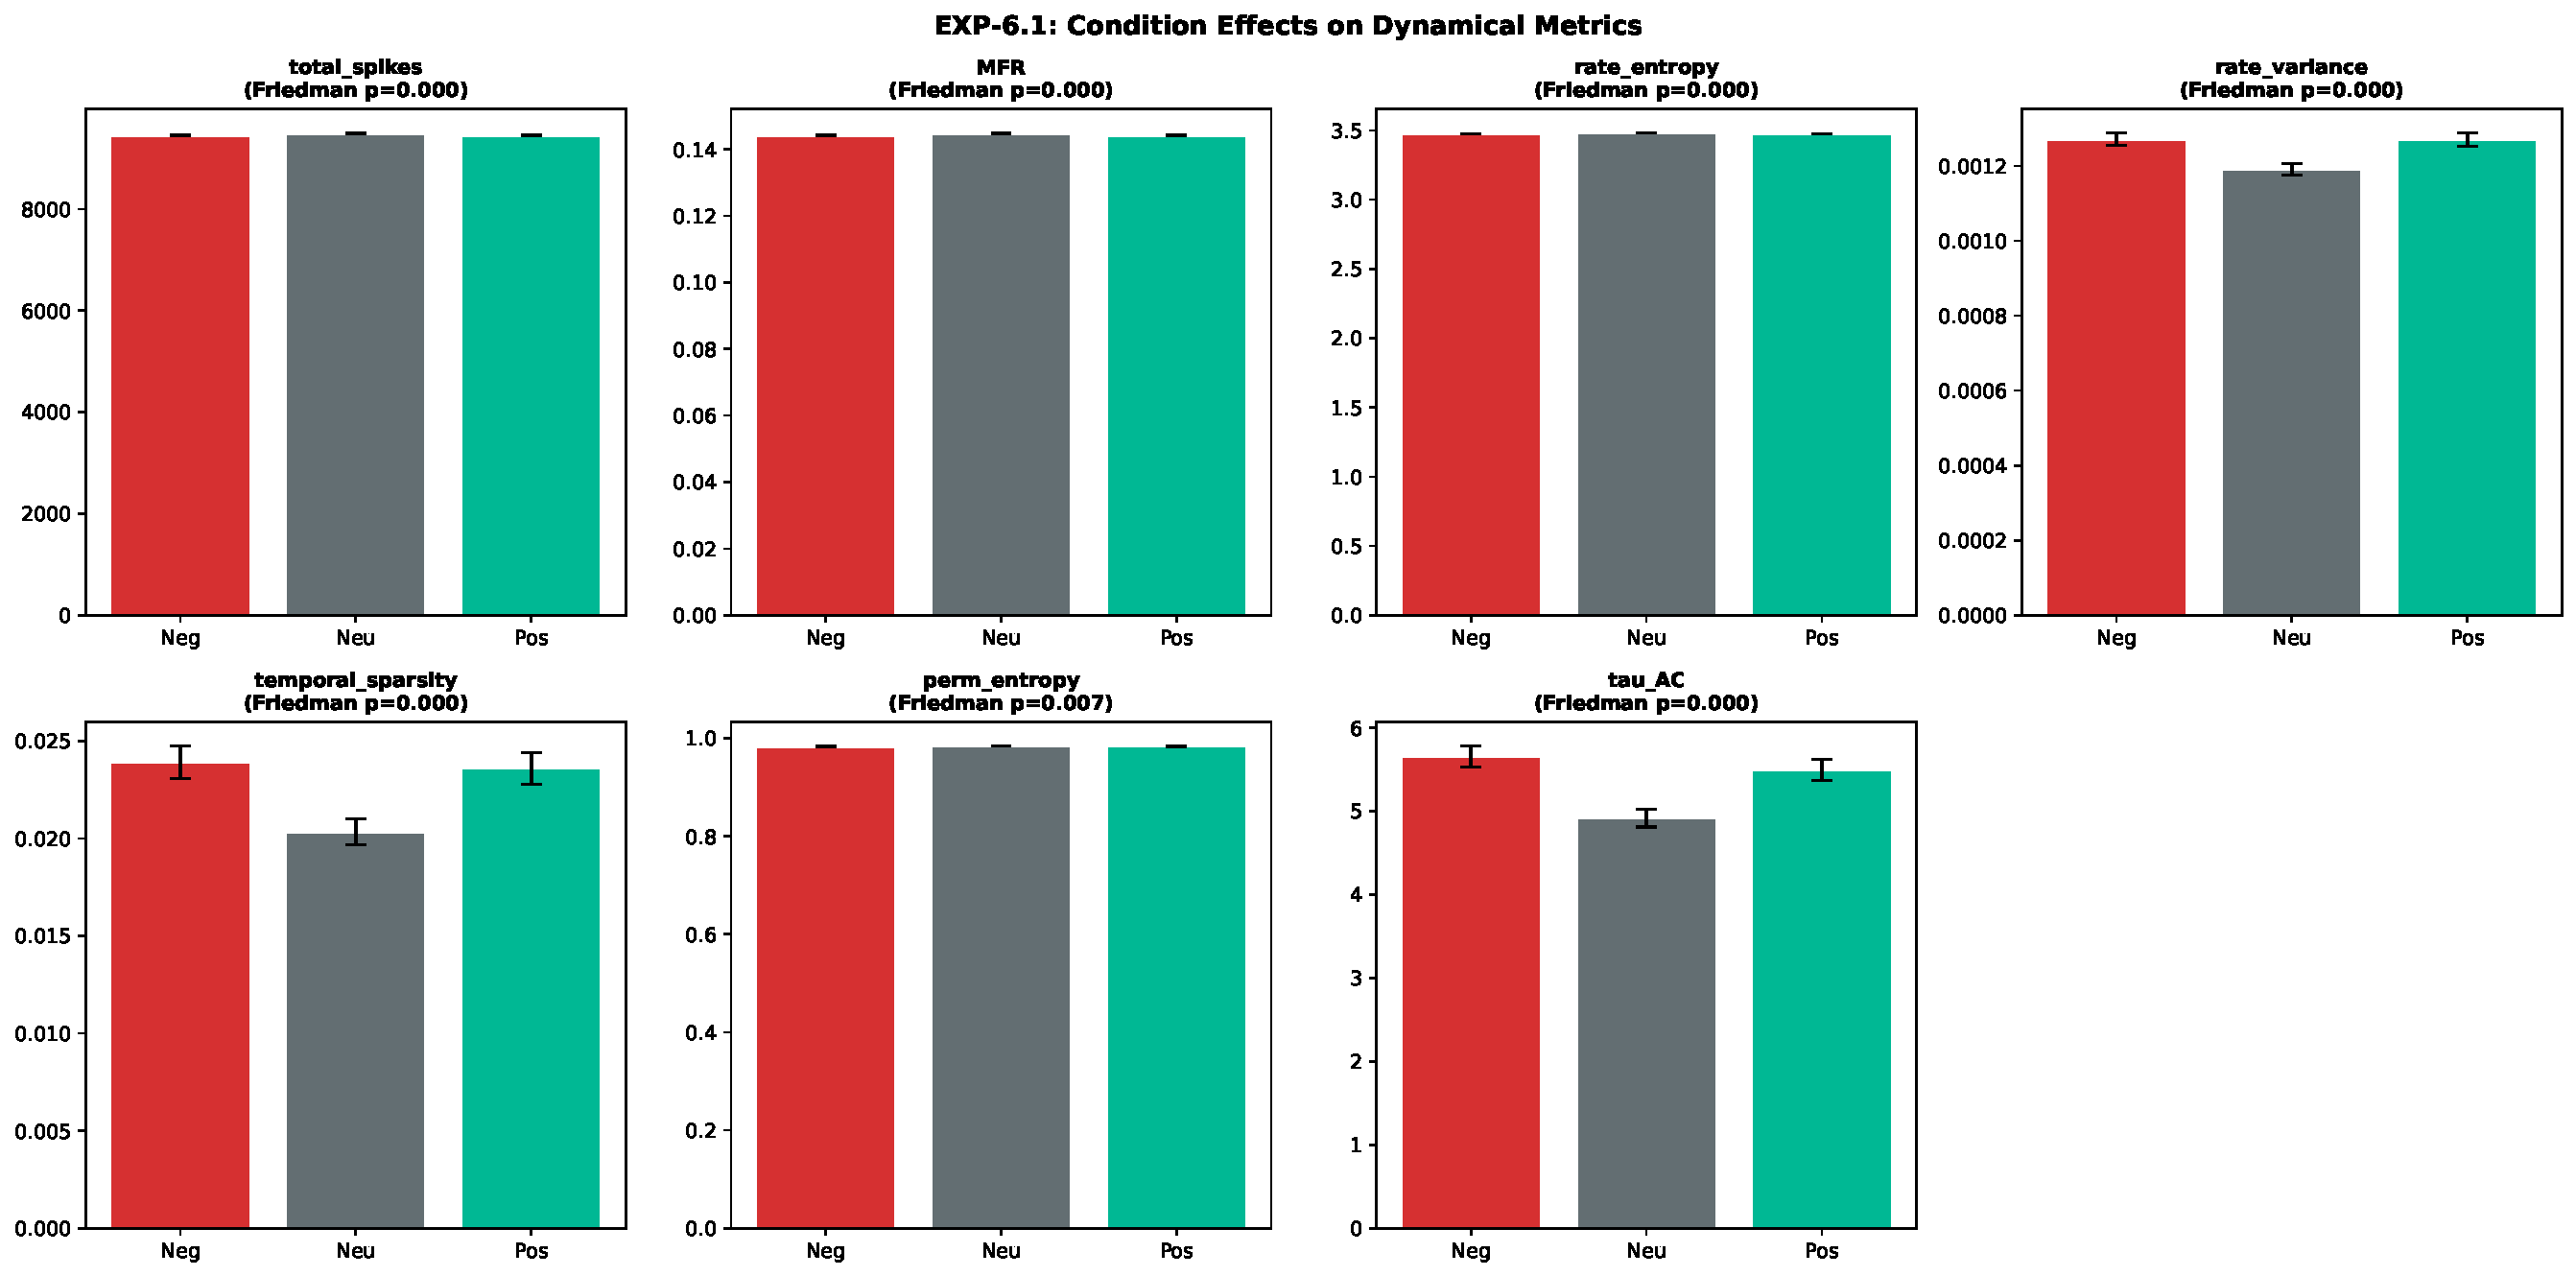
\includegraphics[width=\textwidth]{pictures/chDynamics/fig01_condition_effects.pdf}
    \caption{Exploratory condition comparisons for seven primary dynamical metrics ($N = 211$ participants, Friedman tests). All seven omnibus tests have nominal $p<0.05$. The displayed Negative and Pleasant means are close, while contrasts involving Neutral are larger. The family was not evaluated as a prespecified confirmatory test.}
    \label{fig:ch6_condition_effects}
\end{figure}

\subsection{EXP-6.2: Descriptive Metric-Family Effect-Size Ratio}

For the small Negative--Pleasant contrasts, the mean absolute effect in the two-member temporal-structure family ($\hat{H}_{\pi}$ and $\tau_{AC}$; mean $|d_z|=0.058$) is $2.4$ times the mean in the four-member amplitude-tracking family (mean $|d_z|=0.024$; Figure~\ref{fig:ch6_metric_families}). This is a descriptive ratio of two small, differently sized metric families; it is not a direct inferential test that temporal organization is uniquely responsible for condition encoding.

\begin{figure}[H]
    \centering
    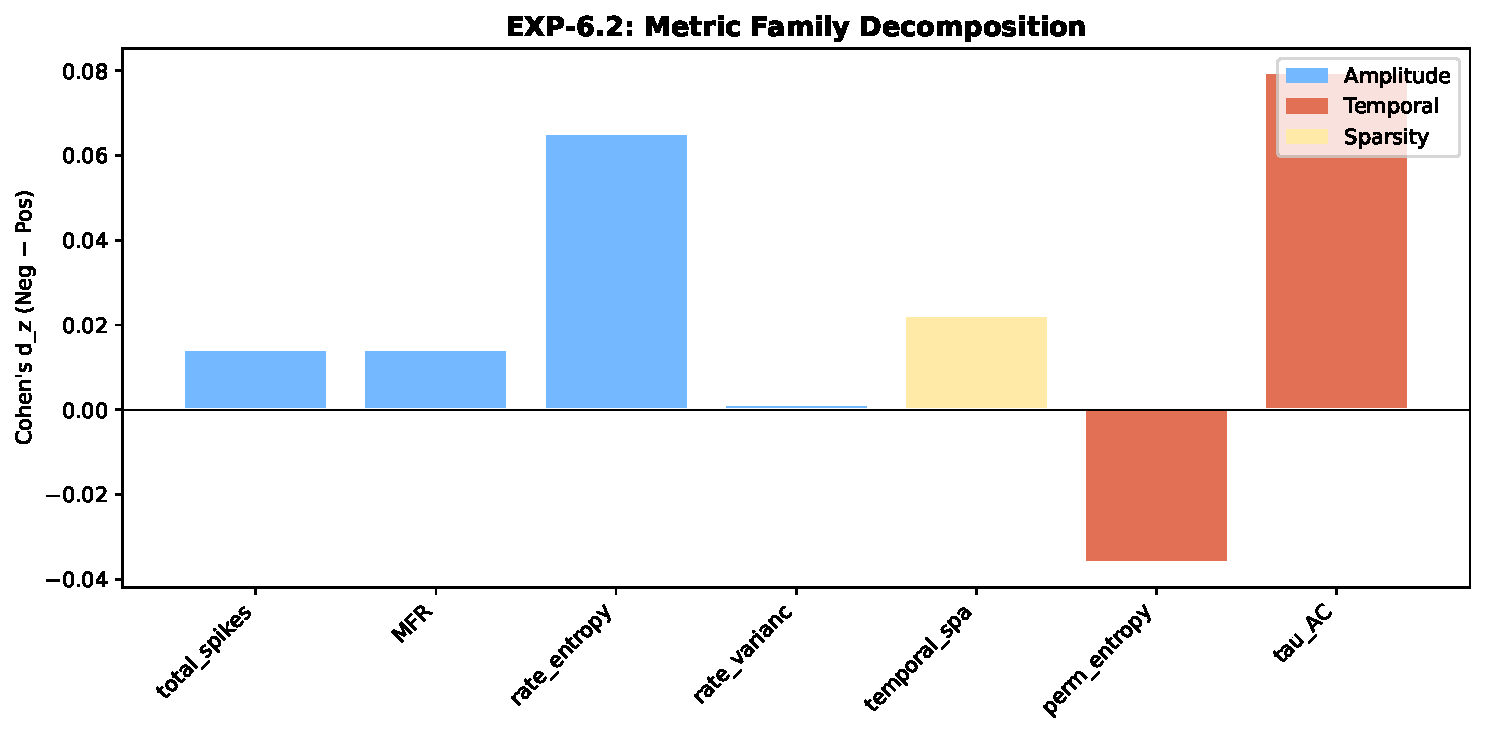
\includegraphics[width=0.85\textwidth]{pictures/chDynamics/fig02_metric_families.pdf}
    \caption{Descriptive metric-family comparison for Negative--Pleasant paired effect sizes ($d_z$). The two temporal-structure metrics have a mean absolute effect $2.4$ times that of the four amplitude-tracking metrics, but all effects in this comparison are small and the family contrast was not directly tested.}
    \label{fig:ch6_metric_families}
\end{figure}

\subsection{EXP-6.3: No Detected Clinical Group Differences}

None of the $49$ metric--group comparisons ($7$ metrics $\times$ $7$ clinical variables) has nominal $p<0.05$ (Figure~\ref{fig:ch6_clinical_heatmap}). The largest observed difference is MDD on $\tau_{AC}$: $5.44$ for MDD versus $5.19$ for non-MDD ($\Delta=+0.24$). These tests provide no evidence of group differences at the sensitivity of this sample; they do not establish equality or absence of smaller effects.

\begin{figure}[H]
    \centering
    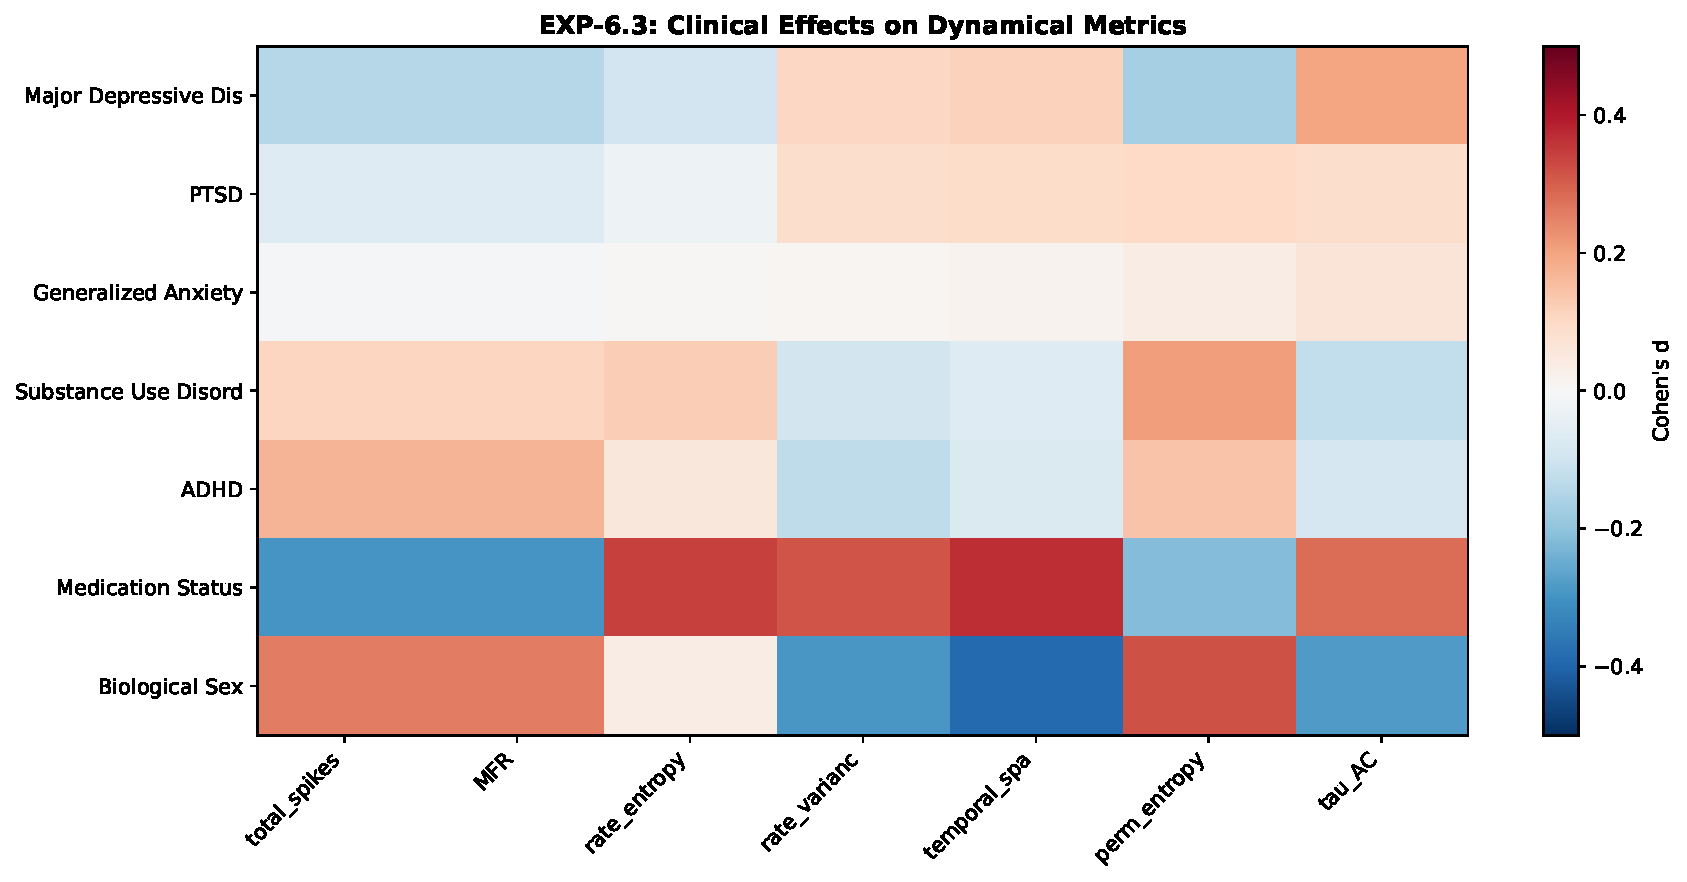
\includegraphics[width=\textwidth]{pictures/chDynamics/fig03_clinical_heatmap.pdf}
    \caption{Exploratory transdiagnostic comparisons for seven dynamical metrics and seven grouping variables. None of the $49$ nominal tests has $p<0.05$. The result is a lack of detected group differences, not evidence that clinical effects are absent.}
    \label{fig:ch6_clinical_heatmap}
\end{figure}

The condition contrasts are larger than the observed channel-averaged clinical contrasts in this cohort. That difference is descriptive: it does not show that the reservoir distinguishes stimuli but not people, and it cannot be compared directly with the broad, partly uncorrected graph search in Chapter~\ref{chap:arspi_net}.

\subsection{EXP-6.4: No Significant Condition \texorpdfstring{$\times$}{by} Clinical Interactions}

Zero of $35$ interaction tests ($7$ metrics $\times$ $5$ clinical variables) has nominal $p<0.05$ (Figure~\ref{fig:ch6_interactions}). The archived sample means for MDD and non-MDD $\tau_{AC}$ reactivity are $+0.24$ and $-0.01$, respectively. Without a supported interaction, that direction is descriptive and does not confirm the hypothesis.

\begin{figure}[H]
    \centering
    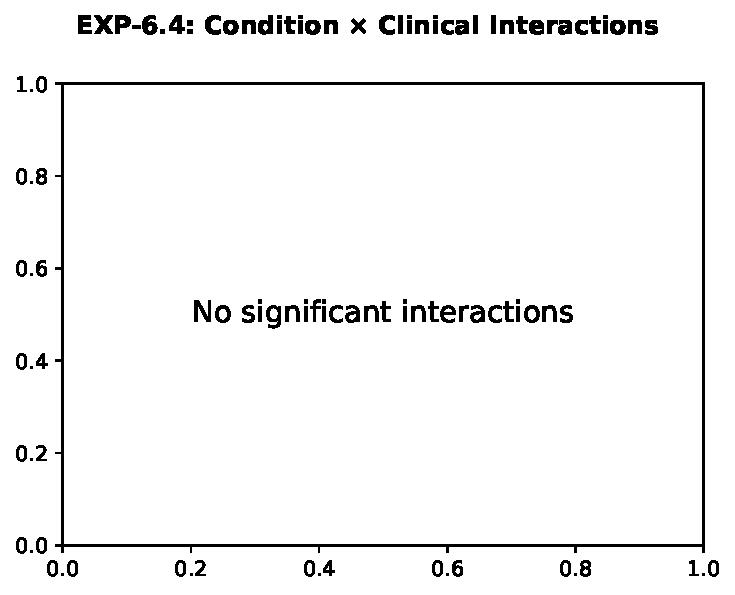
\includegraphics[width=0.85\textwidth]{pictures/chDynamics/fig04_interactions.pdf}
    \caption{Exploratory condition-by-group screens using Negative--Pleasant reactivity. None of the 35 nominal interaction tests has $p<0.05$; displayed directions do not confirm the proposed clinical hypotheses.}
    \label{fig:ch6_interactions}
\end{figure}

\subsection{EXP-6.5: Estimated Operation Counts Are Stable Across Conditions}

The archived analysis shows that total spike count, and therefore the estimated synaptic-operation denominator, varies by approximately $0.5\%$ across conditions at the selected operating point. The earlier trial-level ``bits/spike'' construction used one accuracy-derived numerator for every observation and is not a valid per-trial mutual-information estimate; it is omitted. A fold-safe decoded-information summary would require new out-of-fold predictions after the preprocessing corrections described in Chapter~\ref{chap:arspi_net}. This experiment therefore supports only the narrower observation that gross firing cost is stable across conditions.

\subsection{EXP-6.6: HC vs MDD Hypothesis Tests}

All archived directional comparisons have $p>0.3$ (Figure~\ref{fig:ch6_hc_vs_mdd}). The archived ``HC'' group contains 27 records because five participants with incomplete diagnostic panels were treated as negative; only 22 complete cases are negative for all five primary diagnoses. The resulting HC--MDD contrasts are therefore not valid complete-case control comparisons and are retained only to document the prior analysis. No participant-level $\Phi$ comparison is reported because the operation-normalized decoder summary is defined at the dataset level.

\begin{figure}[H]
    \centering
    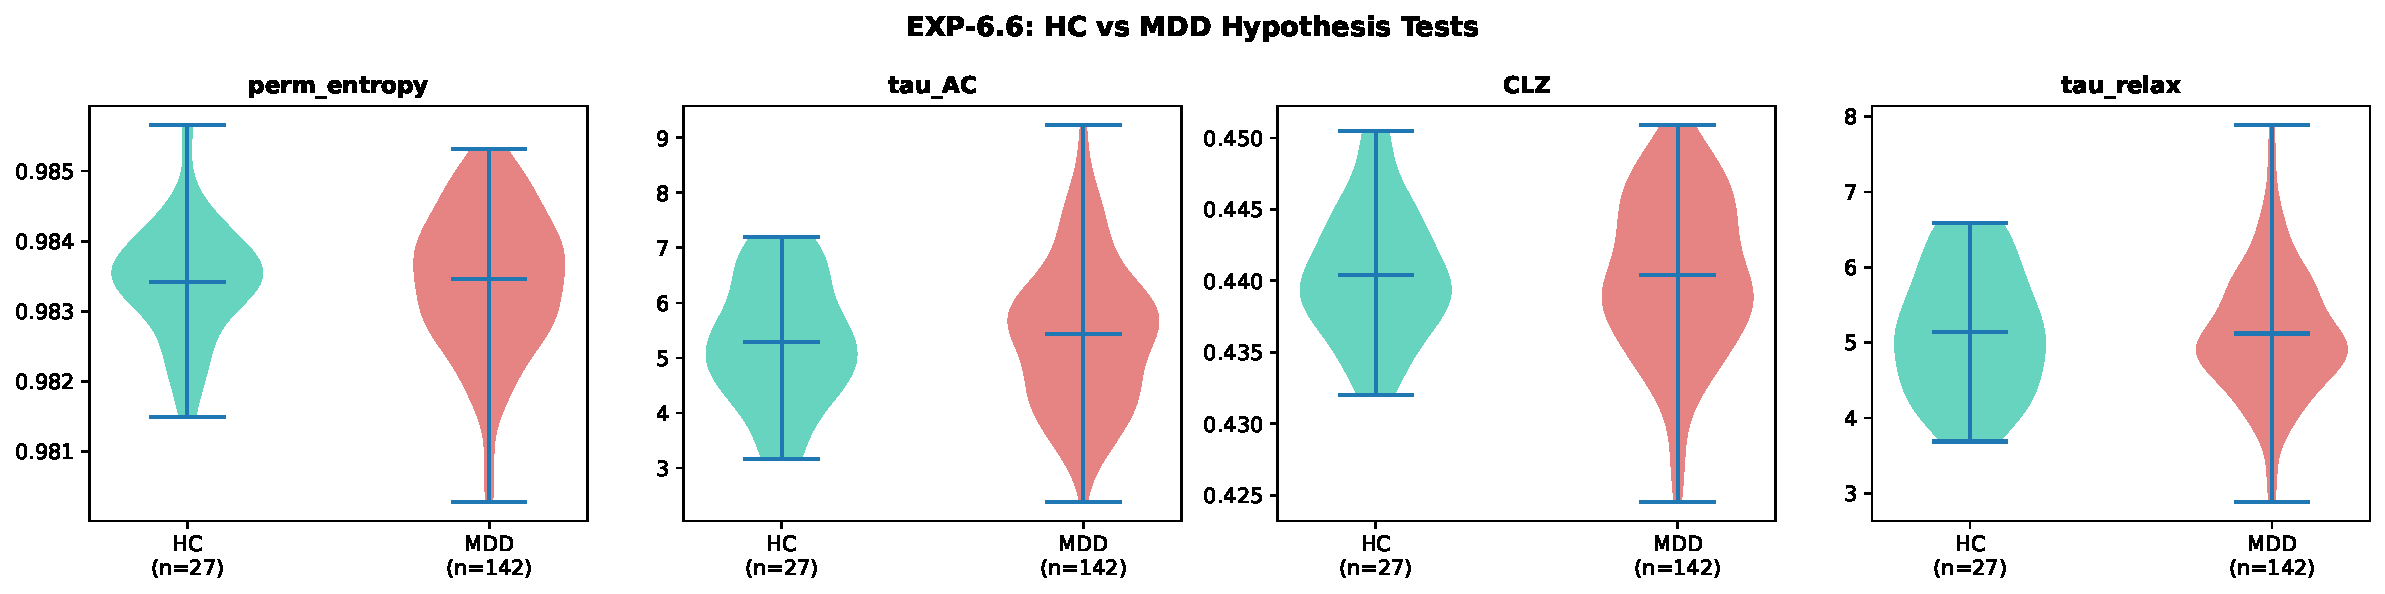
\includegraphics[width=\textwidth]{pictures/chDynamics/fig06_hc_vs_mdd.pdf}
    \caption{Archived HC--MDD screen. The displayed ``HC'' group ($n=27$) includes five participants with incomplete diagnostic panels; the verified complete-case all-negative group has $n=22$. The plotted $\tau_{AC}$ estimate ($d=+0.11$) is therefore descriptive and should be recomputed with the corrected control definition.}
    \label{fig:ch6_hc_vs_mdd}
\end{figure}

The archived point estimates are small ($|d|<0.12$), but the control-definition error and non-significance prevent a directional conclusion. A corrected complete-case analysis must use the 22 verified all-negative participants and report uncertainty without treating a post-hoc detectable-effect calculation as a bound.

\subsection{EXP-6.7: Archived Classifier Results}

The archived three-class classifier using per-channel dynamical features ($238$ dimensions $=34$ channels $\times7$ summaries) has $49.8\%$ balanced accuracy (Figure~\ref{fig:ch6_classification}); the channel-averaged version has $42.2\%$. Adding four auxiliary summaries gives $42.6\%$ in the averaged representation. Because feature and model choices were not evaluated in a fully nested design, these differences are descriptive and do not establish incremental information.

\begin{figure}[H]
    \centering
    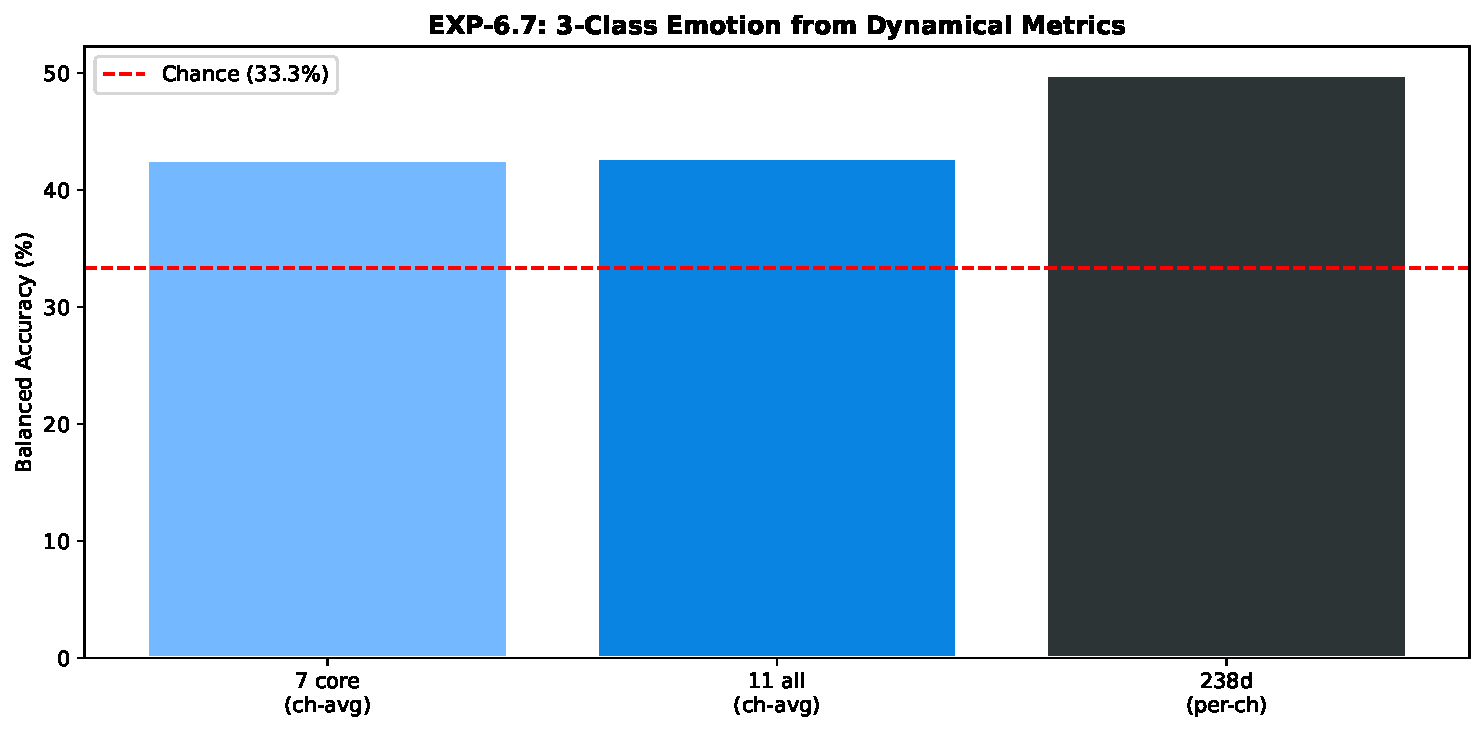
\includegraphics[width=0.75\textwidth]{pictures/chDynamics/fig07_classification.pdf}
    \caption{Archived three-class classification using dynamical summaries. Per-channel features have $49.8\%$ balanced accuracy and channel-averaged features have $42.2\%$. The comparison is descriptive; no nested test establishes the source of the difference.}
    \label{fig:ch6_classification}
\end{figure}

Binary clinical-label estimates using the dynamical summaries are near chance ($49$--$56\%$). The post-hoc maximum for the SUD label is $53.6\%$, which does not establish clinical discrimination. These values provide no basis for claiming that the summaries are clinically sensitive.


\section{Chapter Summary}
\label{sec:dynamics_relationship}

The seven experiments describe the reservoir response using named summaries: total spikes (count), mean firing rate (spikes per neuron per timestep), rate entropy (bits), rate variance, temporal sparsity (fraction of quiescent timesteps), permutation entropy (normalized and dimensionless), and autocorrelation time (timesteps). Their definitions make them inspectable properties of the implemented reservoir response. They are not all physical measurements, and patient-level reliability and clinical actionability are not evaluated.

The findings provide exploratory evidence that these summaries vary with condition. The temporal-structure family has a larger mean absolute Negative--Pleasant effect than the amplitude-tracking family, but the effects are small and the family contrast is descriptive. The archived dynamical-feature classifier reaches $49.8\%$ balanced accuracy. Because model-selection and preprocessing choices were not evaluated in a nested confirmatory design, this value is reported as a descriptive cohort result.

No channel-averaged clinical comparison is detected in EXP-6.3. Per-channel ablation produces near-chance maxima for some diagnoses, but those selected maxima do not establish disorder-specific signals. Chapter~\ref{chap:synthesis} uses the per-channel structure descriptively in the coupling analysis.

Table~\ref{tab:dynamics_relationship_updated} summarizes the relationship between the classification pipeline and the dynamical characterization.

\begin{table}[H]
\centering
\caption{Relationship between the ARSPI-Net classification pipeline and the dynamical characterization.}
\label{tab:dynamics_relationship_updated}
\begin{tabularx}{\textwidth}{>{\raggedright\arraybackslash}p{0.18\textwidth} >{\raggedright\arraybackslash}X >{\raggedright\arraybackslash}X}
\toprule
\textbf{Aspect} & \textbf{Classification (Chapters 3--5)} & \textbf{Dynamical Characterization (This Chapter)} \\
\midrule
Question & Can the system discriminate affective states? & How do reservoir dynamics differ across conditions? \\
Output & Class label $\hat{y}\in\{c_1,\ldots,c_K\}$ & Continuous metric vector $\mathbf{x}\in\mathbb{R}^7$ \\
Condition sensitivity & Archived PCA-dependent estimate; descriptive & Seven nominal Friedman $p<0.05$; exploratory family \\
Clinical sensitivity & Broad exploratory topological search & No detected channel-averaged comparison; near-chance ablation maxima \\
Quantity summarized & Discriminative geometry & Temporal trajectory dynamics \\
\bottomrule
\end{tabularx}
\end{table}


\section{Exploratory Descriptor-to-ERP Alignment}
\label{sec:ch6_erp_alignment}

The seven reservoir summaries have nominal within-cohort condition differences (Section~\ref{sec:ch6_results}). This section reports an exploratory comparison between amplitude-domain analogs and selected ERP scalar summaries. It does not validate a level of explanation fidelity.

Six temporal descriptors were computed from the centered ERP data in the feature window (steps 10--70): mean amplitude (analog of mean firing rate), amplitude variance (analog of spike-count variance), temporal autocorrelation at lag~1 (analog of $\tau_{AC}$), signal complexity (variance of first differences, analog of permutation entropy), peak latency, and temporal asymmetry (early-vs-late energy ratio). The Pearson correlations with classical ERP scalars are:

\begin{table}[H]
\centering
\caption{Exploratory correlations between six amplitude-domain summaries computed in the early feature window and selected ERP scalars. The feature window does not cover the full P300 interval and does not overlap the stated LPP interval, so the correlations are associations rather than component recovery.}
\label{tab:descriptor_erp}
\begin{tabular}{lccc}
\toprule
\textbf{Descriptor} & \textbf{r(P300 amp)} & \textbf{r(LPP amp)} & \textbf{r(P300 lat)} \\
\midrule
Mean amplitude & $+0.647$ & $-0.820$ & $-0.040$ \\
Amplitude variance & $+0.094$ & $-0.069$ & $-0.083$ \\
Temporal autocorrelation & $+0.027$ & $-0.023$ & $-0.133$ \\
Signal complexity & $+0.059$ & $-0.035$ & $+0.046$ \\
Peak latency & $+0.026$ & $-0.018$ & $-0.174$ \\
Temporal asymmetry & $-0.025$ & $+0.022$ & $+0.091$ \\
\bottomrule
\end{tabular}
\end{table}

The early-window mean-amplitude summary has the largest displayed correlations: $r=0.647$ with the P300 scalar and $|r|=0.820$ with the LPP scalar. The largest selected channel correlation is $r=0.837$. Because the early window does not span those components and the strongest channel was selected after inspection, these values are cohort associations and not evidence of component recovery or localization.

The autocorrelation and peak latency descriptors show weak correlations with P300 latency ($r = -0.133$ and $r = -0.174$, respectively). These effect sizes are insufficient for individual-level prediction and provide limited evidence of temporal alignment beyond the mean-amplitude descriptor.

The BSC$_6$ spike-count associations are weaker ($|r|=0.23$ for the LPP scalar and $r=0.33$ for the P300 scalar). The comparison shows that the selected early amplitude summary covaries more strongly with these cohort-level scalars than the selected spike summary; it does not validate clinical explanation fidelity.

NeuCube uses STDP-based connectivity analysis \cite{kasabov_neucube_2014,doborjeh_explainable_2021}; the present summaries instead describe the driven trajectory of a fixed reservoir. For a fixed saved reservoir and input, they are repeatable computational functions. The reported ERP-scalar correlations provide one descriptive comparison, not a validated bridge to physiology and not a head-to-head interpretability evaluation against ProtoPMed-EEG or EEGNet.


\section{Connection to Structure-Function Coupling}
\label{sec:ch6_bridge}

This chapter defines temporal summaries of the driven reservoir. Chapter~\ref{chap:synthesis} compares those summaries with archived graph quantities across the $34$ channel indices using Spearman correlation. The graph quantities inherit the PCA-basis limitations described in Chapter~\ref{chap:arspi_net}; the resulting correlations are descriptive model-to-model associations, not structure--function coupling in the brain.


\section{Summary of Tested Predictions}
\label{sec:dynamics_predictions}

\begin{table}[H]
\centering
\caption{Summary of dynamical predictions and experimental outcomes.}
\label{tab:dynamics_predictions_updated}
\begin{tabularx}{\textwidth}{>{\raggedright\arraybackslash}p{0.20\textwidth} >{\centering\arraybackslash}p{0.10\textwidth} >{\raggedright\arraybackslash}p{0.18\textwidth} >{\raggedright\arraybackslash}X}
\toprule
\textbf{Metric} & \textbf{Symbol} & \textbf{Predicted Direction} & \textbf{Observed Outcome} \\
\midrule
Operation-normalized decoder summary & $\Phi_{dataset}$ & No participant-level direction & Not estimated after fold-safety correction. \\
Lempel--Ziv Complexity & $C_{LZ}$ & $C_{LZ,HC}>C_{LZ,MDD}$ & Effectively zero ($d = +0.004$, $p = 0.57$). \\
Permutation Entropy & $\hat{H}_{\pi}$ & $\hat{H}_{\pi,HC}>\hat{H}_{\pi,MDD}$ & Effectively zero ($d = -0.03$, $p = 0.64$). \\
Relaxation Time & $\tau_{relax}$ & $\tau_{relax,MDD}>\tau_{relax,HC}$ & Opposite direction ($d = -0.02$, $p = 0.56$). \\
Autocorrelation Decay & $\tau_{AC}$ & $\tau_{AC,MDD}>\tau_{AC,HC}$ & Predicted direction ($d = +0.11$, $p = 0.33$). \\
\midrule
\multicolumn{4}{l}{\textit{Exploratory condition comparisons:}} \\
Condition omnibus & all & Condition dependence & Seven nominal Friedman $p<0.05$; no family-level confirmation. \\
Neg vs Pleasant & all & Neg $\neq$ Pleasant & No nominal pairwise result; profiles are similar. \\
\bottomrule
\end{tabularx}
\end{table}

The archived condition screens contain nominal within-participant contrasts. The displayed HC--MDD screen is not a valid complete-case comparison because its $n=27$ control group includes five incomplete diagnostic panels. These analyses therefore cannot establish that condition and person information occupy distinct layers.


\section{Latent Response Organization in the Dynamical Descriptor Space}
\label{sec:ch6_latent_axis}

The final analysis summarizes the $7$-metric by $34$-channel descriptor matrix with PCA and exploratory clustering. It asks how much in-sample variation lies along the leading components and whether the fitted scores are associated with condition or diagnostic metadata.

\subsection{Methods}

Subject-level descriptor vectors were constructed by averaging the seven dynamical metrics across the three conditions for each of the $211$ subjects, yielding a $211\times238$ matrix. Featurewise means and standard deviations were estimated from that subject-averaged matrix, and PCA was fit to the standardized matrix. Condition-specific vectors were standardized with those same featurewise parameters and projected onto the in-sample PC1 loading. The resulting condition test is descriptive of this cohort; PC1 was not learned in an independent sample. Friedman and Bonferroni-corrected Wilcoxon tests assess repeated condition scores. Clinical associations use Mann--Whitney $U$. A median split and several clustering methods are secondary descriptive analyses. Cluster quality is evaluated by silhouette, Davies--Bouldin, and Calinski--Harabasz indices; repeated initializations assess only algorithmic stability, not biological or test--retest reliability.

\subsection{Principal Component Analysis of the Descriptor Space}

In the fitted sample, PC1 explains $19.1\%$ of descriptor variance, while PC2 and PC3 explain $11.5\%$ and $7.7\%$, respectively. The first three components account for $38.3\%$ in total, and $54$ components are needed to reach $90\%$.

PCA signs are arbitrary. For consistency with the condition-score figure, the axis is oriented so that negative scores correspond to higher excitability: mean firing rate ($-0.073$), rate entropy ($-0.085$), permutation entropy ($-0.070$), and active ratio ($-0.078$) point toward that end, while autocorrelation time ($+0.055$) points toward persistence. The label \textbf{excitability--persistence axis} is a descriptive interpretation of these small, channel-distributed loadings rather than a physiological measurement.

\begin{figure}[t]
    \centering
    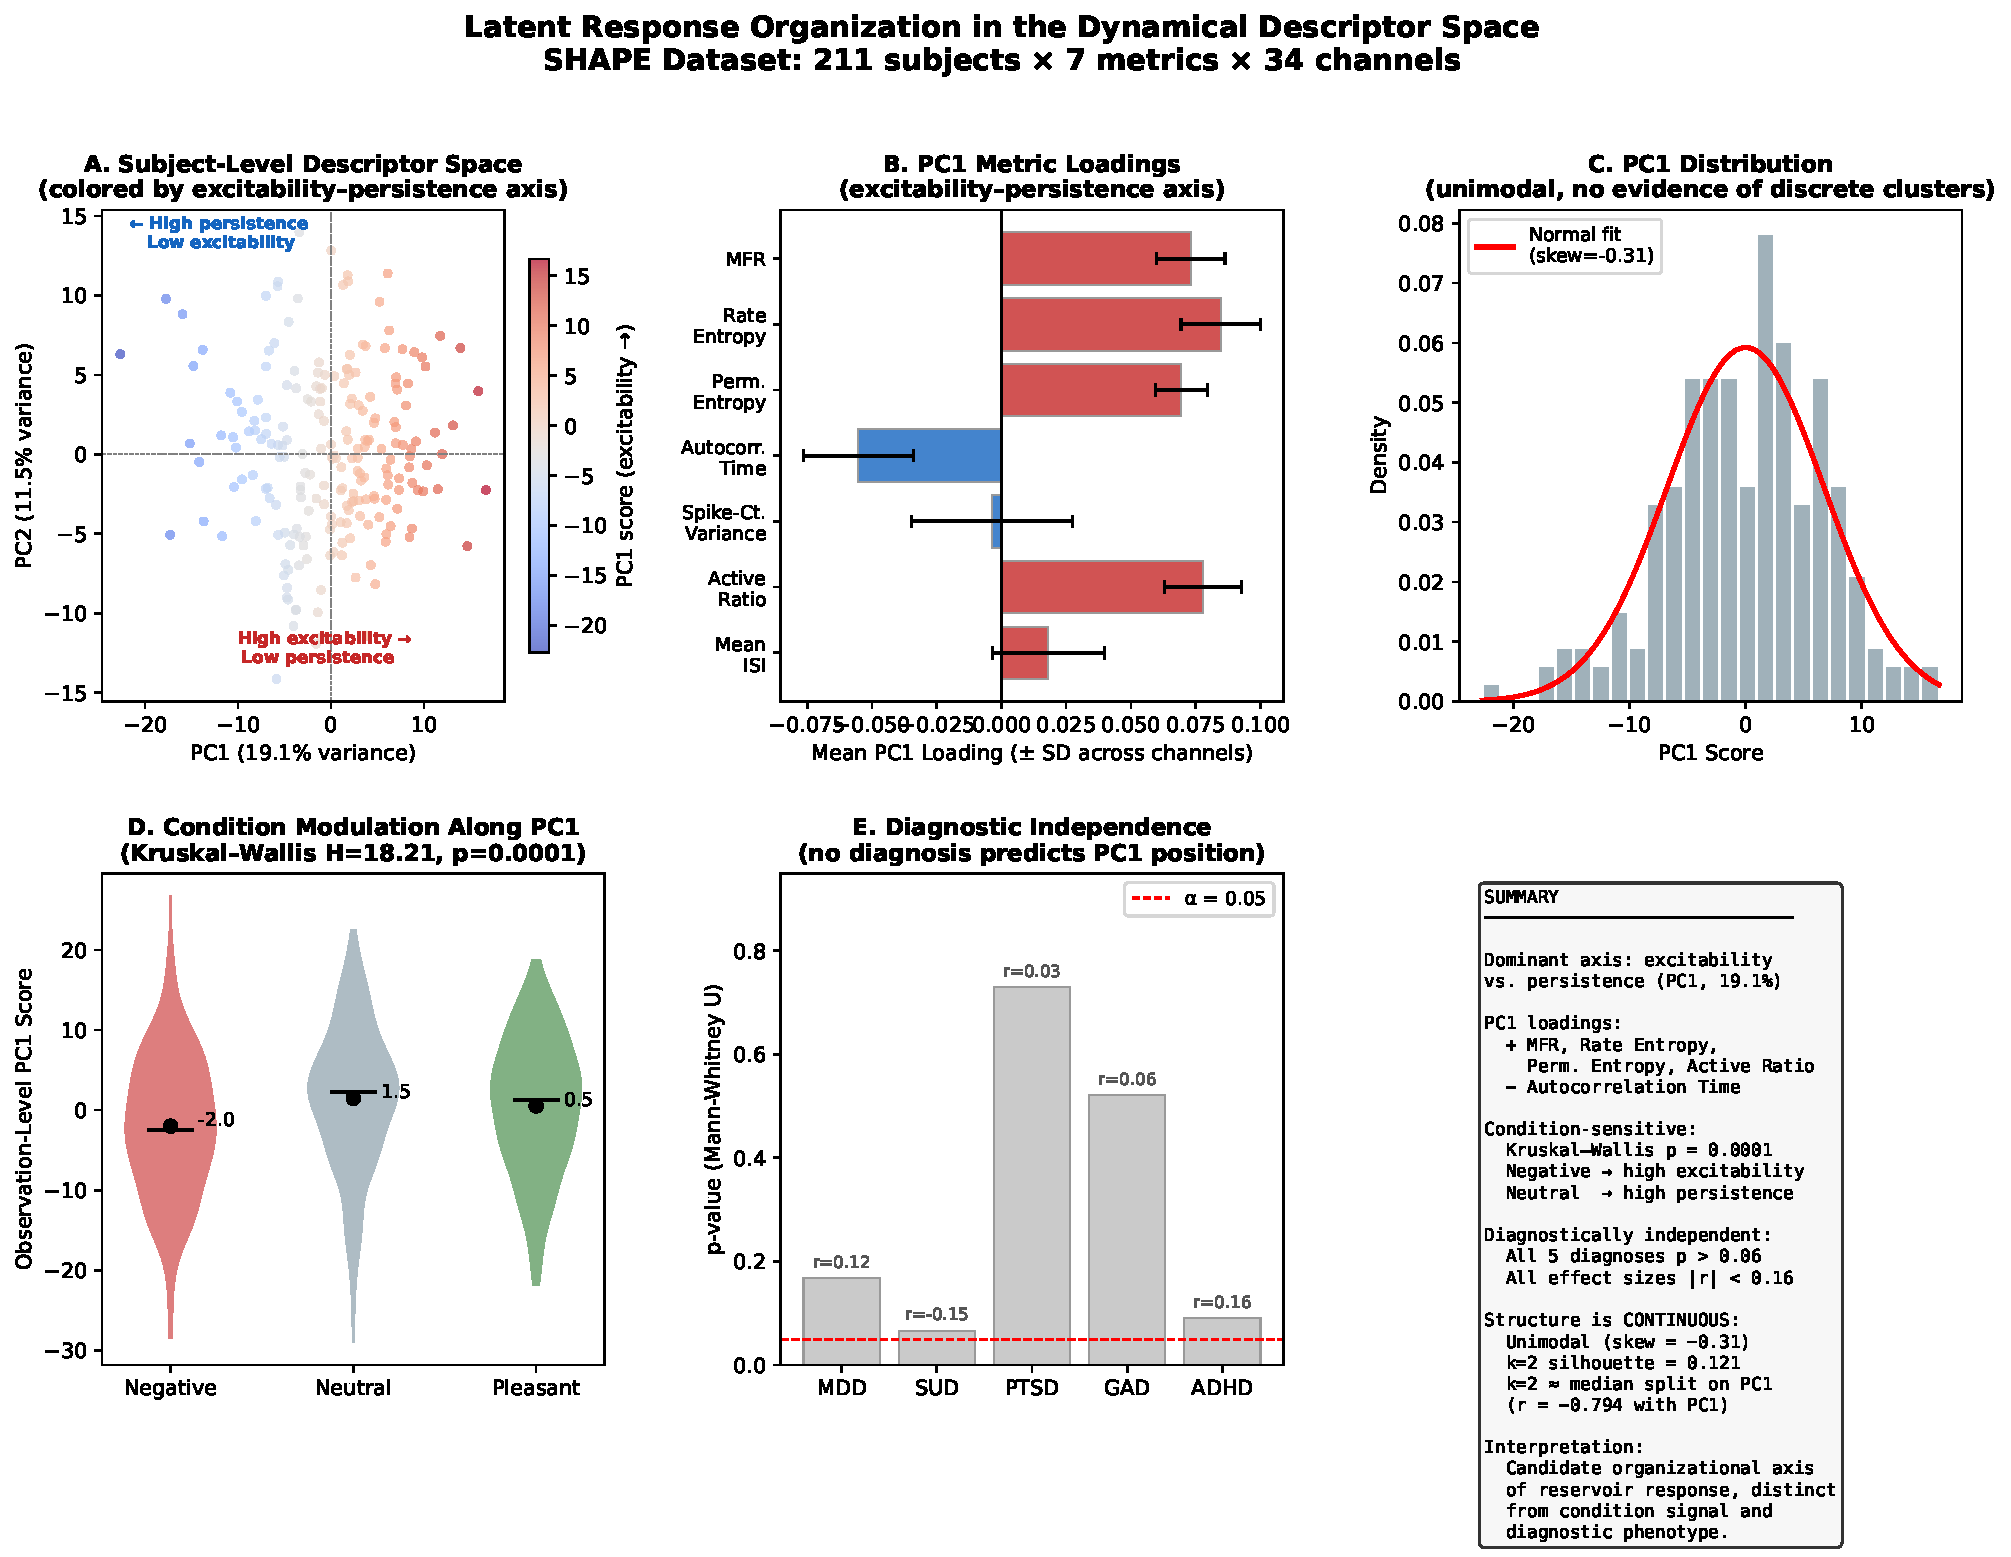
\includegraphics[width=\textwidth]{pictures/chDynamics/fig_latent_axis.pdf}
    \caption{Descriptive organization of the dynamical-summary space. PC1 explains $19.1\%$ of in-sample variance and is labeled excitability--persistence from its small distributed loadings. The condition effect is small ($W=0.057$), the ADHD median-split association is uncorrected, and the one-component BIC preference does not prove a continuous population structure.}
    \label{fig:latent_axis}
\end{figure}

\subsection{Condition Modulation Along the Latent Axis}

To test condition modulation with the correct repeated-measures design, each subject's three condition-specific descriptor vectors were projected onto the PC1 loading vector learned from the subject-level PCA (as described in the Methods), producing three repeated PC1-aligned scores per subject. The Friedman test is the appropriate non-parametric repeated-measures test for this design.

Scores along the in-sample PC1 loading differ by condition (Friedman $\chi^2=24.00$, $p=6\times10^{-6}$, Kendall's $W=0.057$). The oriented means are $-2.00$ for Negative, $+1.47$ for Neutral, and $+0.53$ for Pleasant. Bonferroni-adjusted pairwise tests give small $p$ values for Negative versus the other two conditions and $p=0.29$ for Neutral versus Pleasant. The effect size is small, and because the axis was learned from the same cohort, the result requires out-of-sample confirmation.

\subsection{Association with Psychiatric Diagnosis}

None of the five continuous PC1 group comparisons meets the Bonferroni-adjusted threshold: MDD ($p = 0.17$, $r_{pb} = -0.12$), SUD ($p = 0.07$, $r_{pb} = 0.14$), PTSD ($p = 0.73$, $r_{pb} = -0.01$), GAD ($p = 0.52$, $r_{pb} = -0.04$), and ADHD ($p = 0.09$, $r_{pb} = -0.13$). The sample effect sizes satisfy $|r_{pb}| \leq 0.14$; the adjusted threshold across these five tests is $\alpha_{adj}=0.01$.

As a secondary check, PC1 was split at its sample median and tested against each diagnosis with $\chi^2$ contingency analysis. Four comparisons have Cram\'{e}r's $V<0.08$. ADHD has uncorrected $\chi^2=4.10$, $p=0.043$, and Cram\'{e}r's $V=0.14$, but does not meet the five-test adjusted threshold. Because dichotomization was secondary and loses information, this result is not evidence of an ADHD subgroup. PC1 remains an in-sample description of the descriptor matrix.

\subsection{Discretization and Cluster Structure}

Clustering was evaluated for $k=2$ through $k=6$. The largest silhouette score is only $0.121$ at $k=2$; Gaussian-mixture and spectral variants yield similarly weak separation. The $k=2$ result is seed-stable for the tested initializations (ARI $=1.00$) and strongly associated with PC1 ($r=-0.794$). This is algorithmic consistency in the same data, not biological reliability, and the weak silhouette does not support discrete subpopulations.

A one-component Gaussian mixture has lower BIC than a two-component model ($\Delta\text{BIC}=-14.5$ in favor of one). Together with the weak silhouette, this provides no evidence for a natural two-group boundary. It does not prove that the population distribution is continuous or that the tentative axis has physiological meaning.

\subsection{Summary}

PC1 explains $19.1\%$ of the in-sample descriptor variance and has a small condition association ($W=0.057$). Continuous diagnosis associations are small, and the uncorrected ADHD median-split result does not survive adjustment. BIC favors one component and the $k=2$ silhouette is weak ($0.121$), so the data provide no clear evidence of discrete groups. The ``excitability--persistence'' label is a tentative description of loadings and requires out-of-sample and test--retest evaluation.

\newpage
\chapter{Synthesis: Comparing Temporal Dynamics and Spatial Topology}
\label{chap:synthesis}

\section{Introduction}
\label{sec:ch7_intro}

This chapter compares two families of derived summaries: per-channel reservoir dynamics (Chapter~\ref{chap:dynamics}) and graph topology (Chapter~\ref{chap:arspi_net}). Their electrode-wise association is called coupling. Because both families are transformations of the same trial-averaged EEG epoch, association does not establish a common latent neural mechanism or independence from shared preprocessing.

Chapter~\ref{chap:dynamics} reported condition-associated dynamical summaries, and Chapter~\ref{chap:arspi_net} reported descriptive graph summaries and exploratory clinical comparisons. The strongest nominal SUD comparison had parametric $p=0.0004$, but its label-permutation result was $p=0.073$. These results motivate a cross-summary analysis; they do not establish that one family uniquely represents condition and the other uniquely represents persons.

Related neuroimaging work examines relationships between local functional properties and network topology \cite{Deco2015,honey_network_2007,suarez_linking_2020}. Here $\kappa$ is only a norm of 14 within-epoch, cross-electrode rank correlations. It summarizes association among the derived quantities and has no direction, physiological unit, or demonstrated clinical utility.

The chapter reports archived four-category analyses (Threat, Mutilation, Cute, Erotic) and a separate three-condition analysis (Negative, Neutral, Pleasant). These are not replications: the input grouping, preprocessing, and archived reservoir implementations differ. In particular, the original four-category script omitted the post-spike threshold subtraction and nonnegative floor used by the three-condition pipeline. The audited script now uses the common update, but raw four-category EEG was unavailable for regeneration. Cross-analysis numerical differences are therefore descriptive and cannot be attributed to granularity alone.

Five exploratory analyses compare observed coupling with an electrode-permutation null, decompose sample sums of squares, inspect category differences, compare diagnosis-defined groups, and evaluate linear readouts built from the two descriptor families.


\section{Mathematical Framework}
\label{sec:ch7_framework}

\subsection{Data Objects}

For each subject $s \in \{1,\ldots,211\}$ and category $c \in \{\text{Threat, Mutilation, Cute, Erotic}\}$, two per-electrode descriptor matrices are constructed from the same $1229 \times 34$ category-level trial-averaged EEG epoch.

The \textbf{dynamical profile matrix} $\mathbf{D}_{s,c}\in\mathbb{R}^{34\times7}$ contains total spikes, mean firing rate, rate entropy, rate variance, temporal sparsity, permutation entropy~$\hat{H}_\pi$, and autocorrelation decay~$\tau_{AC}$ for each channel. These are descriptive metrics selected in Chapter~\ref{chap:dynamics}. Each column is computed after driving a fixed reservoir ($N_{res}=256$, $\beta=0.05$, $M_{th}=0.5$, seed~42) with a z-scored single-channel epoch. The archived four-category numbers were generated with the legacy reset update disclosed above.

The \textbf{topological profile matrix} $\mathbf{T}_{s,c} \in \mathbb{R}^{34 \times 2}$ contains two primary graph metrics for each electrode: weighted node strength and weighted clustering coefficient (Onnela formula) \cite{onnela_intensity_2005}. These are extracted from a $34 \times 34$ theta-band ($4$--$8$~Hz) time-averaged phase concentration (tPLV) matrix \cite{lachaux_measuring_1999}. Because the available data are category-level trial averages (one epoch per subject per category), the tPLV is computed as within-epoch phase concentration,
\begin{equation}
\label{eq:tplv}
\text{tPLV}_{ij} = \left|\frac{1}{T}\sum_{t=1}^{T} e^{j(\phi_i(t) - \phi_j(t))}\right|,
\end{equation}
where $\phi_i(t)$ is the instantaneous phase of the theta-filtered signal at channel~$i$. This is not classical trial-to-trial phase locking; it is within-epoch phase-difference concentration. Weighted strength and Onnela clustering are used as two summaries of the resulting dense weighted matrix \cite{rubinov_complex_2010}. Their reliability was not estimated here, and the unlabeled channel montage prevents anatomical interpretation.

\subsection{Coupling Measures}

The within-subject coupling matrix is defined by electrode-wise Spearman rank correlations between the two descriptor families:
\begin{equation}
\label{eq:coupling_C}
\mathbf{C}_{s,c} \in \mathbb{R}^{7 \times 2}, \quad (\mathbf{C}_{s,c})_{jk} = \rho_S(\mathbf{D}_{s,c}[:,j],\;\mathbf{T}_{s,c}[:,k]),
\end{equation}
where $\rho_S$ denotes Spearman correlation computed across the 34 electrodes. Each entry of $\mathbf{C}_{s,c}$ quantifies how one dynamical metric covaries with one topological metric across the electrode array for a specific subject and category.

The scalar coupling strength is the normalized Frobenius norm:
\begin{equation}
\label{eq:kappa}
\kappa_{s,c} = \frac{\|\mathbf{C}_{s,c}\|_F}{\sqrt{p \cdot q}} = \frac{1}{\sqrt{14}}\sqrt{\sum_{j=1}^{7}\sum_{k=1}^{2}(\mathbf{C}_{s,c})_{jk}^2}.
\end{equation}
This normalization maps $\kappa$ to $[0,1]$ and enables comparison across configurations with different $p$ and $q$. A $\kappa$ near zero indicates that the dynamical and topological descriptor families are unaligned across electrodes; a $\kappa$ near one indicates that every dynamical metric is strongly rank-correlated with every topological metric.

Spearman $\mathbf{C}_{s,c}$ and scalar $\kappa_{s,c}$ are the primary coupling instruments throughout this chapter. Canonical Correlation Analysis (CCA) is available as a secondary multivariate summary but is not used for primary inference due to the modest ratio of electrodes ($N_c = 34$) to variables ($p + q = 9$), which produces upward-biased canonical correlations in small samples \cite{wang_cca_2020}.

\subsection{Null Model}

The channel-permutation null shuffles the row indices of $\mathbf{T}_{s,c}$ relative to $\mathbf{D}_{s,c}$, breaking channel correspondence while preserving marginal values. For each of 5,000 permutations~$\pi$, a null coupling $\kappa_{s,c}^{(\pi)}$ is computed. The per-observation Monte Carlo $p$-value is
\begin{equation}
p_{s,c} = \frac{1 + \#\{\kappa_{s,c}^{(\pi)} \ge \kappa_{s,c}\}}{1 + 5000}.
\end{equation}
This null treats channel labels as exchangeable. Spatial smoothness and shared-reference effects can violate that assumption, so the result tests this particular label-shuffling null rather than a general null of no neurophysiological coupling.


\section{Data and Experimental Protocol}
\label{sec:ch7_protocol}

All experiments use the Stress, Health, and the Psychophysiology of Emotion (SHAPE) Community dataset \cite{noauthor_shape_2018}: $N = 211$ subjects (excluding subject~127), four IAPS subcategories (Threat, Mutilation, Cute, Erotic), yielding 844 subject--category observations. Each observation is a $1229 \times 34$ category-level trial-averaged EEG epoch at 1024~Hz, consistent with the data format in Chapters~\ref{chap:dynamics} and~5.

For each observation, the reservoir processes all 34 channels independently (28,696 total reservoir runs across the dataset). The tPLV matrix is computed from the same 34-channel epoch via theta-band filtering (3rd-order Butterworth, $4$--$8$~Hz) and Hilbert-transform phase extraction. Complete data for the five primary diagnoses are available for 206 of 211 subjects; 22 of those 206 are negative for all five (MDD, PTSD, SUD, GAD, and ADHD). The value 27 results only if the five incomplete records are incorrectly treated as diagnosis-negative and is not used. The supplied full-panel comorbidity variable has mean 2.8 (rounded) across 211 records.

Analyses use Wilcoxon signed-rank for paired summaries, Mann--Whitney~$U$ for group comparisons, and selected permutation tests. Bonferroni correction is applied only within explicitly stated families. Repeated categories from the same subject are not independent; where a test uses all subject--category rows without clustering or subject-level reduction, its $p$-value is labeled anti-conservative and descriptive.


\section{Experiment 7.1: Coupling Existence}
\label{sec:exp7_coupling}

\subsection{Mathematical Motivation}

Both $\mathbf{D}_{s,c}$ and $\mathbf{T}_{s,c}$ are derived from the same underlying EEG epoch through different transformations: the reservoir maps each channel's temporal signal into a dynamical descriptor, while the tPLV maps all pairwise phase relationships into a topological descriptor. If an electrode that participates in strong phase-locked interactions also drives the reservoir into a distinctive dynamical regime, then $\mathbf{D}_{s,c}$ and $\mathbf{T}_{s,c}$ will be rank-correlated across the electrode array. The observable quantities are the $7 \times 2$ coupling matrix $\mathbf{C}_{s,c}$, the scalar $\kappa_{s,c}$, and their distribution across 844 observations relative to the electrode-permutation null.

\subsection{Experimental Design}

For each of 844 subject--category observations, $\mathbf{C}_{s,c}$ and $\kappa_{s,c}$ are compared with 5,000 channel permutations. The archived group test applies a one-sided Wilcoxon test to all 844 differences between observed $\kappa$ and its null median. Because four rows come from each subject, that extremely small $p$-value is anti-conservative. An archived subject-level test compared mean $\kappa$ with zero; because $\kappa$ is a nonnegative norm with a positive finite-sample null expectation, that is not a valid confirmatory null test. A valid subject-level reanalysis would average $\kappa_{\mathrm{obs}}-\kappa_{\mathrm{null}}$ within subject or permute channel correspondence jointly within subject. The source package does not contain the raw inputs needed to regenerate the corrected four-category results.

\subsection{Raw Observation}

\begin{figure}[htbp]
\centering
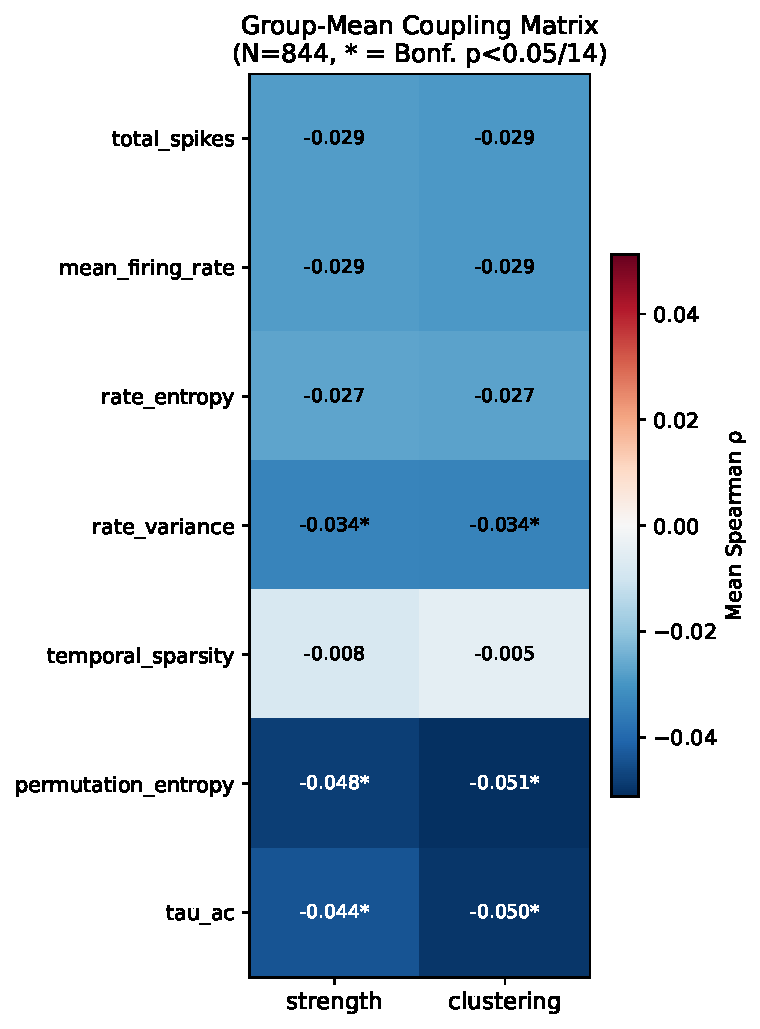
\includegraphics[width=0.65\textwidth]{pictures/chSynthesis/fig7_A1_mean_coupling_matrix.pdf}
\caption{Mean signed coupling matrix across 844 subject--category observations (211 subjects, four categories). All 14 sample means are negative. Asterisks reproduce archived Bonferroni-adjusted row-level tests, but those tests treat repeated categories as independent and are therefore descriptive.}
\label{fig:mean_C}
\end{figure}

All 14 sample-mean correlations are negative, ranging from $-0.005$ to $-0.051$ (Figure~\ref{fig:mean_C}). These are small cross-channel associations. They do not show that greater phase concentration causes a change in reservoir dynamics, and averaging conceals the mixed signs observed in individual matrices.

\begin{figure}[htbp]
\centering
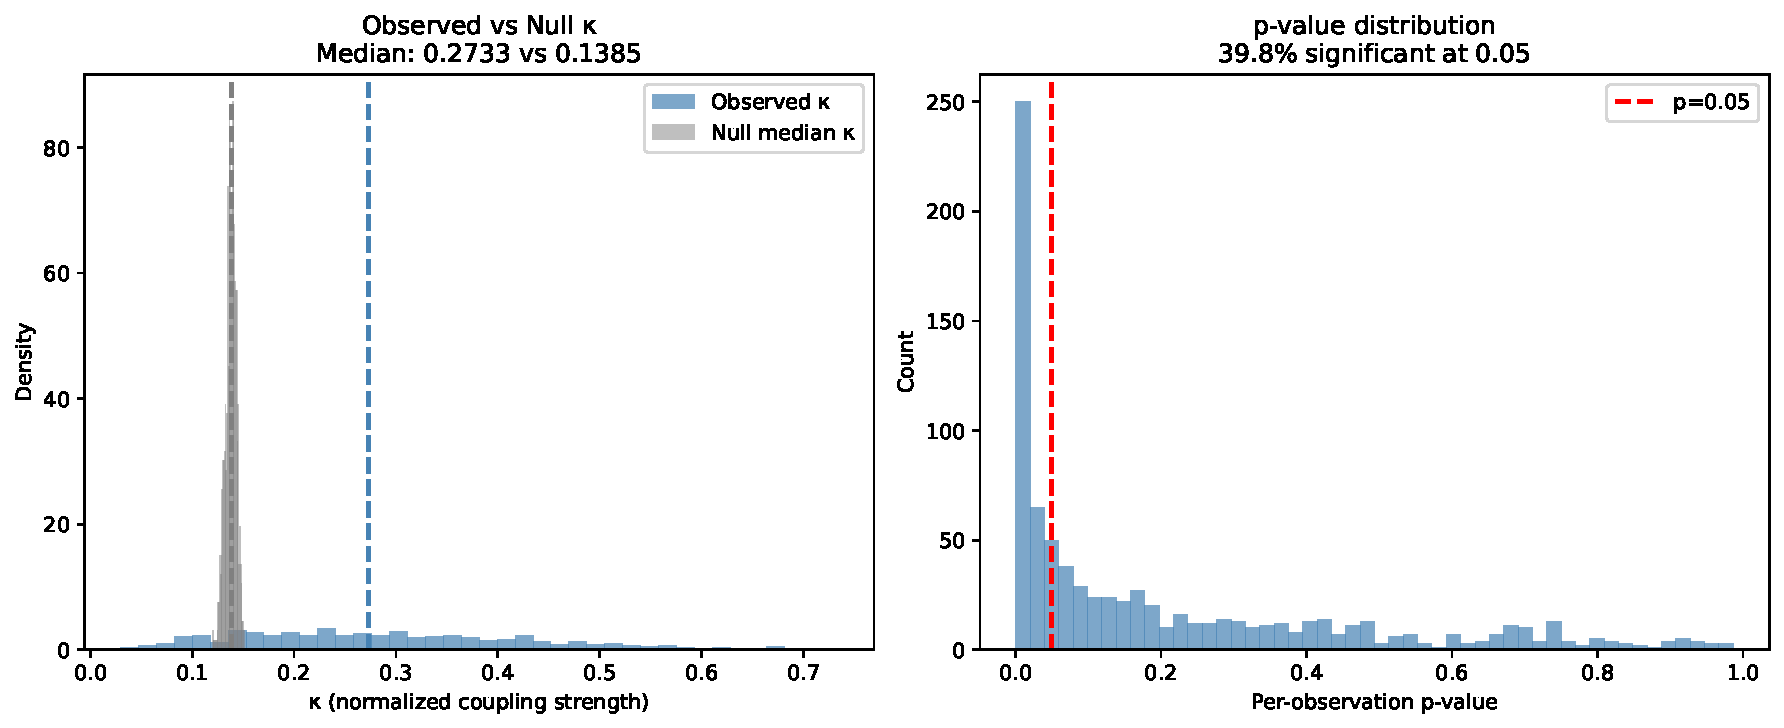
\includegraphics[width=0.95\textwidth]{pictures/chSynthesis/fig7_A2_kappa_vs_null.pdf}
\caption{Observed $\kappa$ and each observation's channel-permutation null median (left), with per-observation Monte Carlo $p$-values (right). Rows are repeated within subject and the null assumes exchangeable channel labels.}
\label{fig:kappa_null}
\end{figure}

The observed median is 0.273 (range 0.030--0.734), compared with a median of 0.139 for the per-observation null medians; 39.8\% of observations have Monte Carlo $p<0.05$ under the stated channel-permutation null. This percentage is descriptive and is not corrected across 844 tests.

\begin{figure}[htbp]
\centering
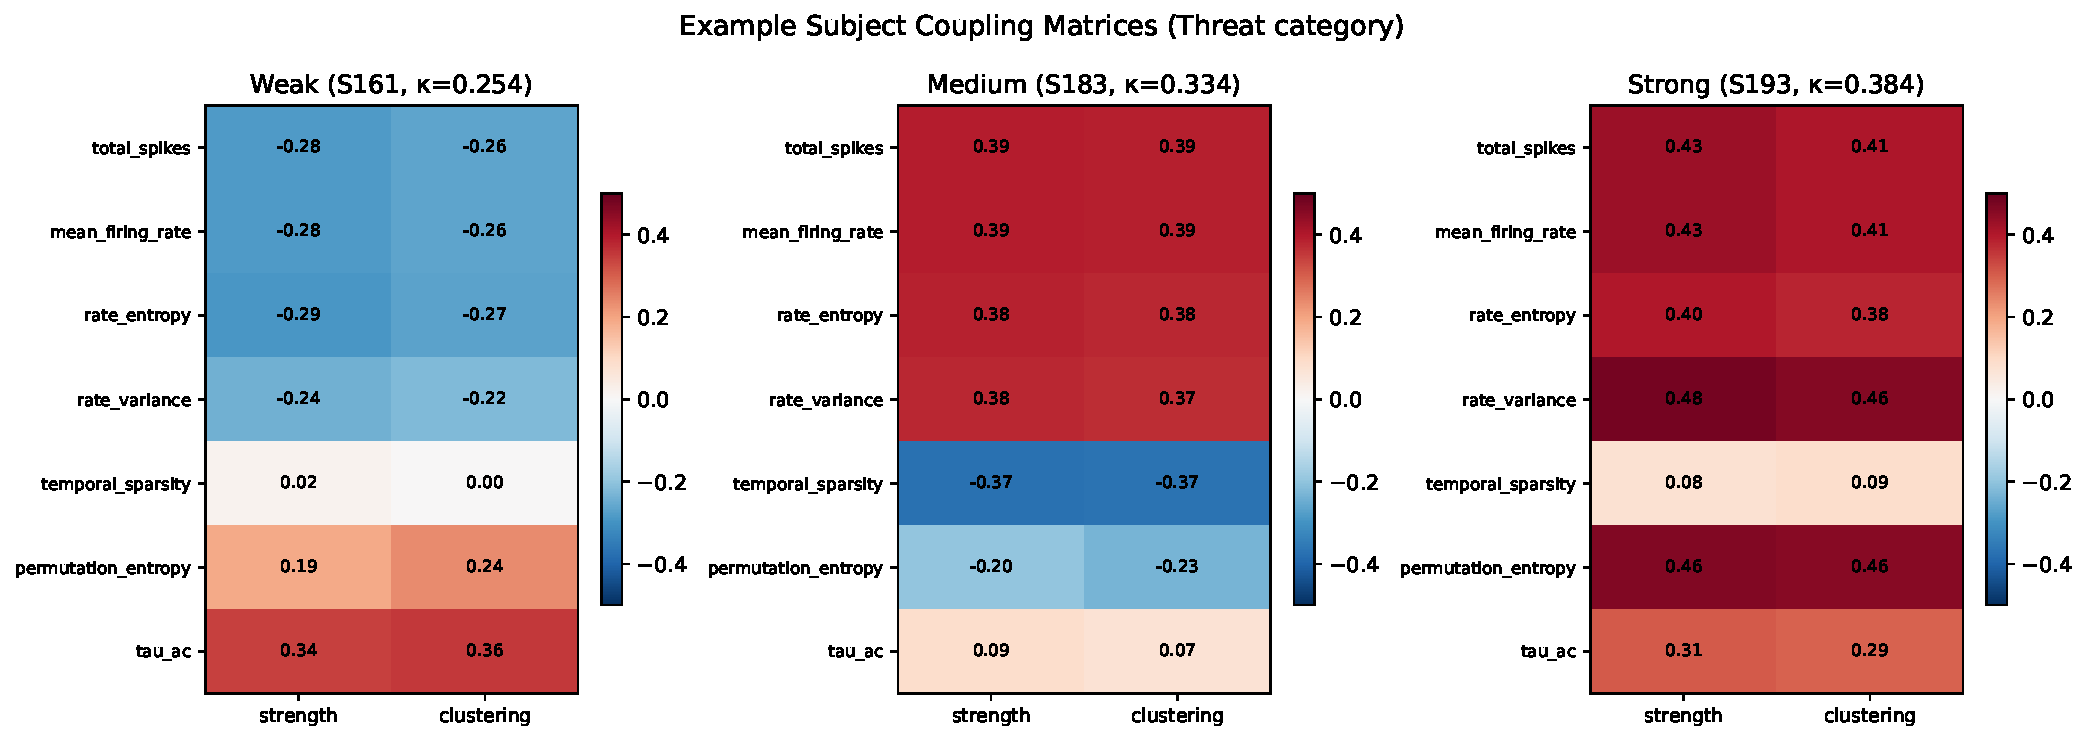
\includegraphics[width=0.95\textwidth]{pictures/chSynthesis/fig7_A3_example_subjects.pdf}
\caption{Example coupling matrices for three subjects (Threat category), selected at the 10th, 50th, and 90th percentiles of subject-mean $\kappa$. Individual-level coupling matrices show substantial inter-subject heterogeneity in both magnitude and sign pattern.}
\label{fig:example_subjects}
\end{figure}

Figure~\ref{fig:example_subjects} illustrates heterogeneity among three selected observations. Subject~161 ($\kappa = 0.254$) has negative spike-metric correlations but positive $\tau_{AC}$ correlations. Subject~183 ($\kappa = 0.334$) has the opposite pattern, and Subject~193 ($\kappa = 0.384$) has positive correlations throughout. These examples show that averaging correlations with different signs can reduce the group mean; they do not estimate the prevalence of any pattern in the population.

\subsection{Quantitative Analysis}

The archived row-level Wilcoxon test on $\kappa_{\text{obs}}-\kappa_{\text{null median}}$ gives $W=338{,}144$ and $p=4.98\times10^{-113}$; the mean difference divided by its row-level standard deviation is 1.063. Repeated rows make the $p$-value anti-conservative, and the standardized difference is not an independent-subject effect size. The descriptive shift applies only to the specified permutation null.

\begin{table}[htbp]
\centering
\caption{Coupling existence summary (Experiment~7.1).}
\label{tab:coupling_existence}
\small
\begin{tabular}{lcccc}
\toprule
\textbf{Statistic} & \textbf{Observed} & \textbf{Null median} & \textbf{$d_z$} & \textbf{$p$} \\
\midrule
Median $\kappa$ & 0.273 & 0.139 & 1.063 & $4.98 \times 10^{-113}$ \\
\% observations $p < 0.05$ & 39.8\% & 5.0\% (expected) &, &, \\
\% observations $p < 0.01$ & 23.6\% & 1.0\% (expected) &, &, \\
\bottomrule
\end{tabular}
\end{table}

The archived row-level tests flag four of 14 cells after within-matrix Bonferroni correction: permutation entropy and $\tau_{AC}$ paired with both topology summaries. The mean correlations are only $-0.044$ to $-0.051$, and the tests ignore repeated categories, so these cells are candidates for subject-level replication rather than confirmed alignments.

\subsection{Signal-Processing Interpretation}

One possible explanation is that channels with concentrated theta-band phase relationships also have more regular temporal structure, which the reservoir summaries reflect. However, tPLV, signal amplitude/spectrum, common reference, filtering, and the reservoir transform are all potential shared causes. The analysis did not measure ``input diversity'' or isolate any of these mechanisms.

The data-processing inequality does not identify the cause or direction of these correlations \cite{cover_elements_2006}; it only bounds information under deterministic transformation.

The next analysis partitions sample sums of squares in $\kappa$. This is a descriptive decomposition, not evidence that subject or category causally ``drives'' the statistic.


\section{Experiment 7.2: Variance Decomposition of Coupling Strength}
\label{sec:exp7_variance}

\subsection{Mathematical Motivation}

An archived Chapter~5 decomposition assigned 62.6\% of embedding sums of squares to subject and 8.7\% to condition, but those PCA features were fitted globally and are retained only as descriptive context. Here the balanced two-way decomposition $\kappa_{s,c}=\mu+\alpha_s+\beta_c+\varepsilon_{s,c}$ partitions sample sums of squares. It does not identify latent sources of variance or establish trait stability.

\subsection{Experimental Design}

The 844 $\kappa_{s,c}$ values are decomposed into subject, category, and residual sums of squares. Category labels are permuted within subject 5,000 times. ICC(3,1) \cite{shrout_intraclass_1979} summarizes rank consistency across four \emph{different stimulus categories}; it is not test--retest reliability because the four columns are not repeated measurements under the same condition.

\subsection{Raw Observation}

\begin{figure}[htbp]
\centering
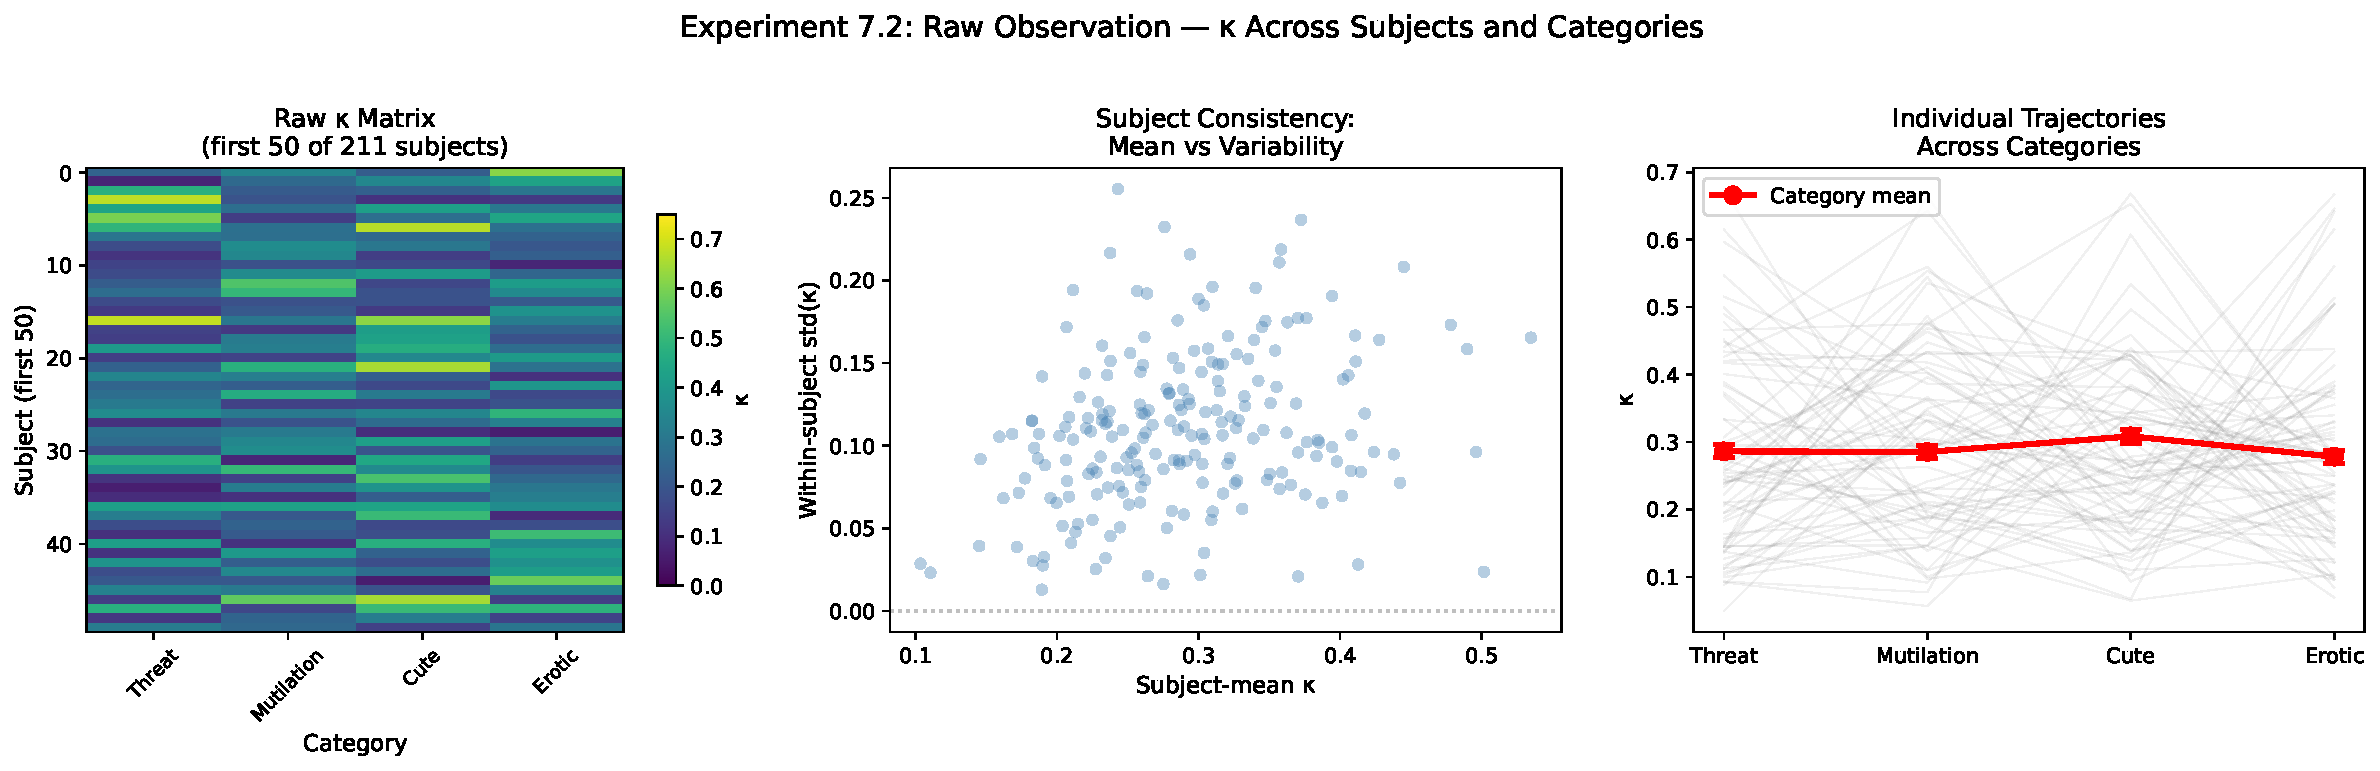
\includegraphics[width=0.95\textwidth]{pictures/chSynthesis/fig7_B1_raw_observation.pdf}
\caption{Raw observation of $\kappa$ across subjects and categories. Left: $\kappa$ matrix for the first 50 subjects (rows) $\times$ 4 categories (columns). Center: subject-mean $\kappa$ versus within-subject standard deviation. Right: individual subject trajectories across categories (gray) with category means (red). Within-subject variability (mean std $= 0.110$) exceeds between-subject variability (std of subject means $= 0.077$).}
\label{fig:raw_kappa_matrix}
\end{figure}

The category means span a narrow range: Cute ($\bar{\kappa} = 0.309$), Threat ($0.286$), Mutilation ($0.285$), Erotic ($0.278$). The between-category spread (max minus min mean) is 0.030. Within-subject standard deviation of $\kappa$ across the four categories averages 0.110, 1.43 times the between-subject standard deviation of 0.077. The individual trajectories in Figure~\ref{fig:raw_kappa_matrix} show extensive crossing: a subject with high $\kappa$ under Threat may have low $\kappa$ under Cute, and vice versa.

\begin{figure}[htbp]
\centering
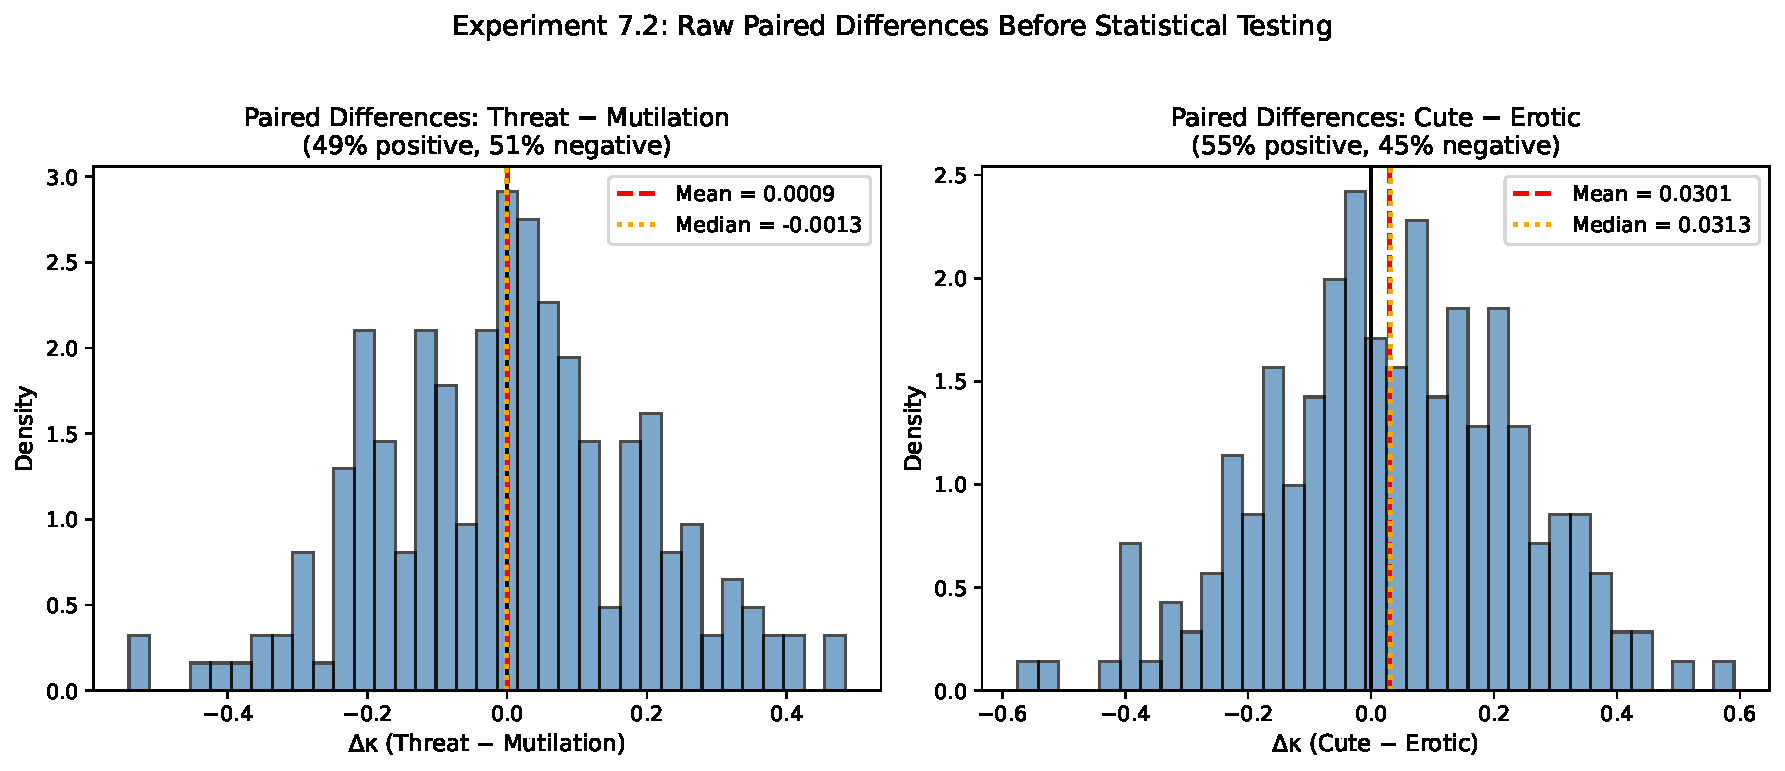
\includegraphics[width=0.95\textwidth]{pictures/chSynthesis/fig7_B2_raw_paired_differences.pdf}
\caption{Raw paired differences in $\kappa$ before statistical testing. Left: Threat $-$ Mutilation (centered on zero, 49.3\% positive). Right: Cute $-$ Erotic (shifted positive, 55.5\% positive, mean $\Delta\kappa = +0.030$).}
\label{fig:raw_paired_diff}
\end{figure}

The observed Threat--Mutilation mean difference is near zero, while the Cute--Erotic sample mean is positive. Whether that contrast exceeds the prespecified multiplicity-adjusted null is considered below.

\subsection{Quantitative Analysis}

\begin{figure}[htbp]
\centering
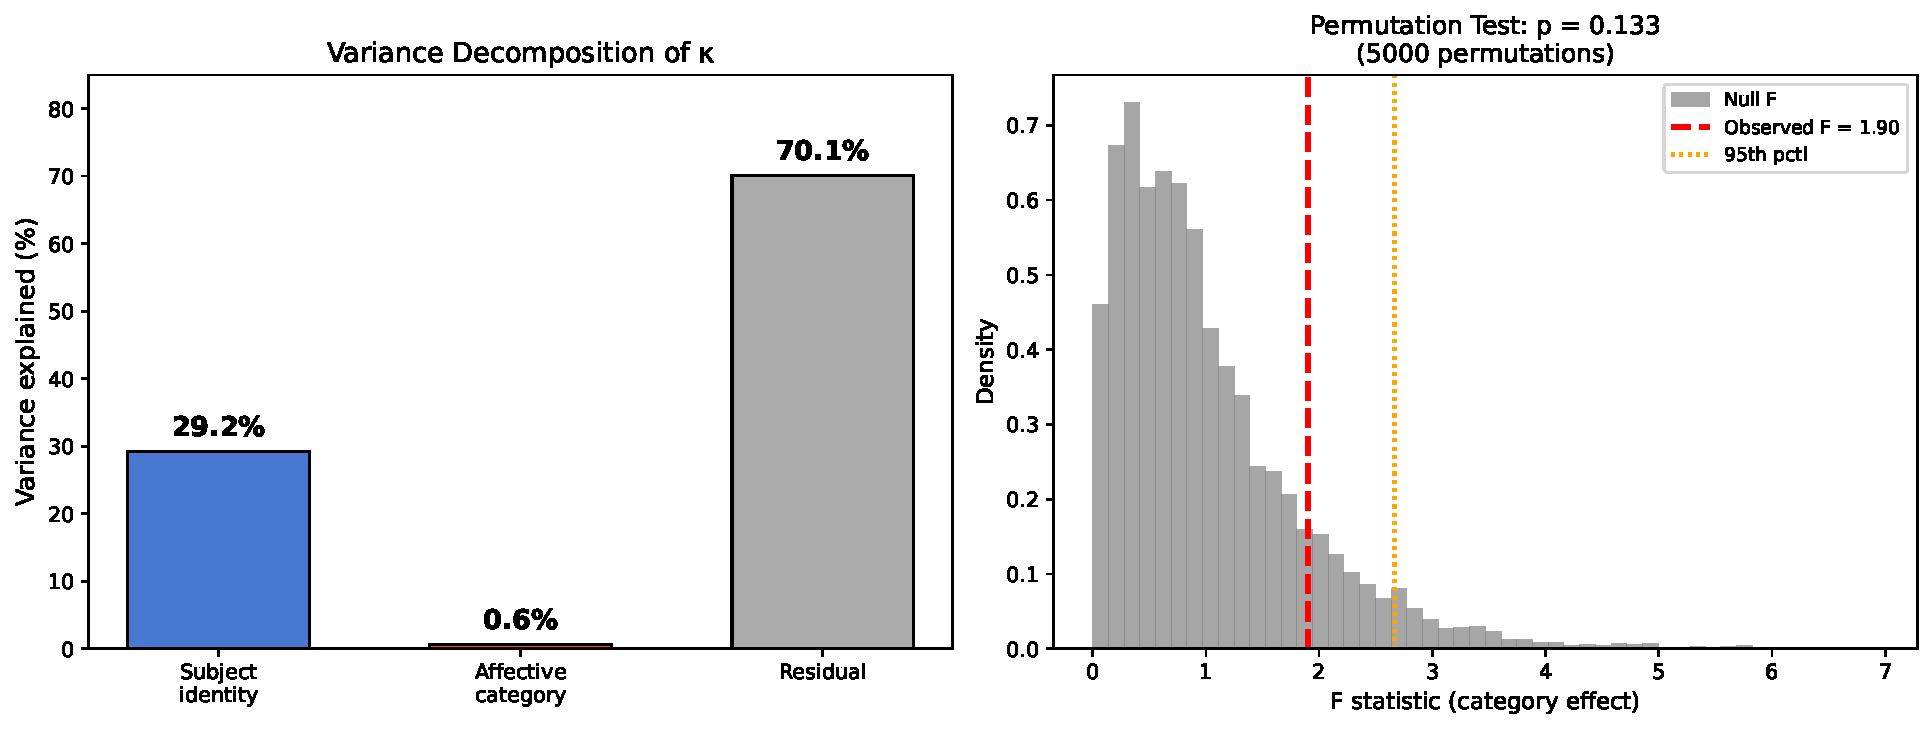
\includegraphics[width=0.95\textwidth]{pictures/chSynthesis/fig7_B3_variance_decomposition.pdf}
\caption{Left: variance decomposition of $\kappa$ into subject (29.2\%), category (0.6\%), and residual (70.1\%) components. Right: permutation null for the category $F$-statistic. The observed $F = 1.90$ falls below the 95th percentile of the null ($p = 0.133$).}
\label{fig:variance_decomp}
\end{figure}

\begin{table}[htbp]
\centering
\caption{Variance decomposition of $\kappa_{s,c}$ (Experiment~7.2).}
\label{tab:variance_decomp}
\small
\begin{tabular}{lcccc}
\toprule
\textbf{Component} & \textbf{\% Variance} & \textbf{$F$} & \textbf{$p$ (permutation)} \\
\midrule
Subject identity & 29.2\% &, &, \\
Affective category & 0.6\% & 1.90 & 0.133 \\
Residual & 70.1\% &, &, \\
\bottomrule
\end{tabular}
\end{table}

The sample sums-of-squares fractions are 29.2\% for subject, 0.6\% for category, and 70.1\% residual (Table~\ref{tab:variance_decomp}; Figure~\ref{fig:variance_decomp}). The category permutation test gives $F=1.90$, $p=0.133$, and the Friedman test gives $\chi^2=3.22$, $p=0.359$. ICC(3,1) across the four different categories is 0.059, indicating little consistency of relative ordering across those category-specific measurements; it does not prove statistical independence or poor test--retest reliability.

Threat--Mutilation gives $\Delta\kappa=-0.001$, $p=0.965$; Cute--Erotic gives $\Delta\kappa=+0.031$, $p=0.025$ without correction for the multiple planned and exploratory contrasts reported in this chapter. Because the omnibus category test is not significant, the latter is treated as a nominal exploratory result.

\subsection{Interpretation and Significance}

The subject fraction is smaller than the archived Chapter~5 fraction, but the underlying variables and preprocessing differ, so the percentages are not directly comparable. The coupling norm should not be said to ``strip away'' individual differences on this basis.

The low cross-category ICC shows that relative subject ordering changes across categories. Trait stability would require repeated sessions or repeated measurements within condition, which are unavailable.

The 70.1\% residual combines subject--category interaction, measurement error, preprocessing effects, and all unmodeled structure. It cannot be labeled genuine observation-specific neural variability without replication.

The Cute--Erotic $\kappa$ difference raises a natural question: when coupling strength increases for Cute relative to Erotic, which specific dynamical-topological relationships are driving the change?


\section{Experiment 7.3: Category-Conditioned Coupling Structure}
\label{sec:exp7_category}

\subsection{Mathematical Motivation}

The scalar $\kappa$ compresses a $7 \times 2$ matrix into one number. A Cute--Erotic difference could be spread across the 14 correlations or concentrated in a subset of cells. Chapter~\ref{chap:dynamics} grouped the descriptors into amplitude-associated summaries (total spikes, firing rate, rate entropy, rate variance) and temporal-structure summaries ($\hat{H}_\pi$, $\tau_{AC}$). The present analysis describes whether the largest sample differences occur in either group; it does not test a distinct biological pathway. The observable quantities are the 14 cell-level paired differences $\Delta\mathbf{C}_{jk} = \mathbf{C}_{\text{Cute},jk} - \mathbf{C}_{\text{Erotic},jk}$ tested with paired Wilcoxon across $N = 211$ subjects.

\subsection{Experimental Design}

For each of the two within-valence contrasts (Cute $-$ Erotic, Threat $-$ Mutilation), 14 paired Wilcoxon tests are computed across 211 subjects. Bonferroni correction within each contrast family yields $\alpha_{\text{corrected}} = 0.05/14 = 0.00357$. A secondary pattern-level test computes the Frobenius norm of the mean $\Delta\mathbf{C}$ against a sign-flip permutation null (5,000 permutations).

\subsection{Raw Observation}

\begin{figure}[htbp]
\centering
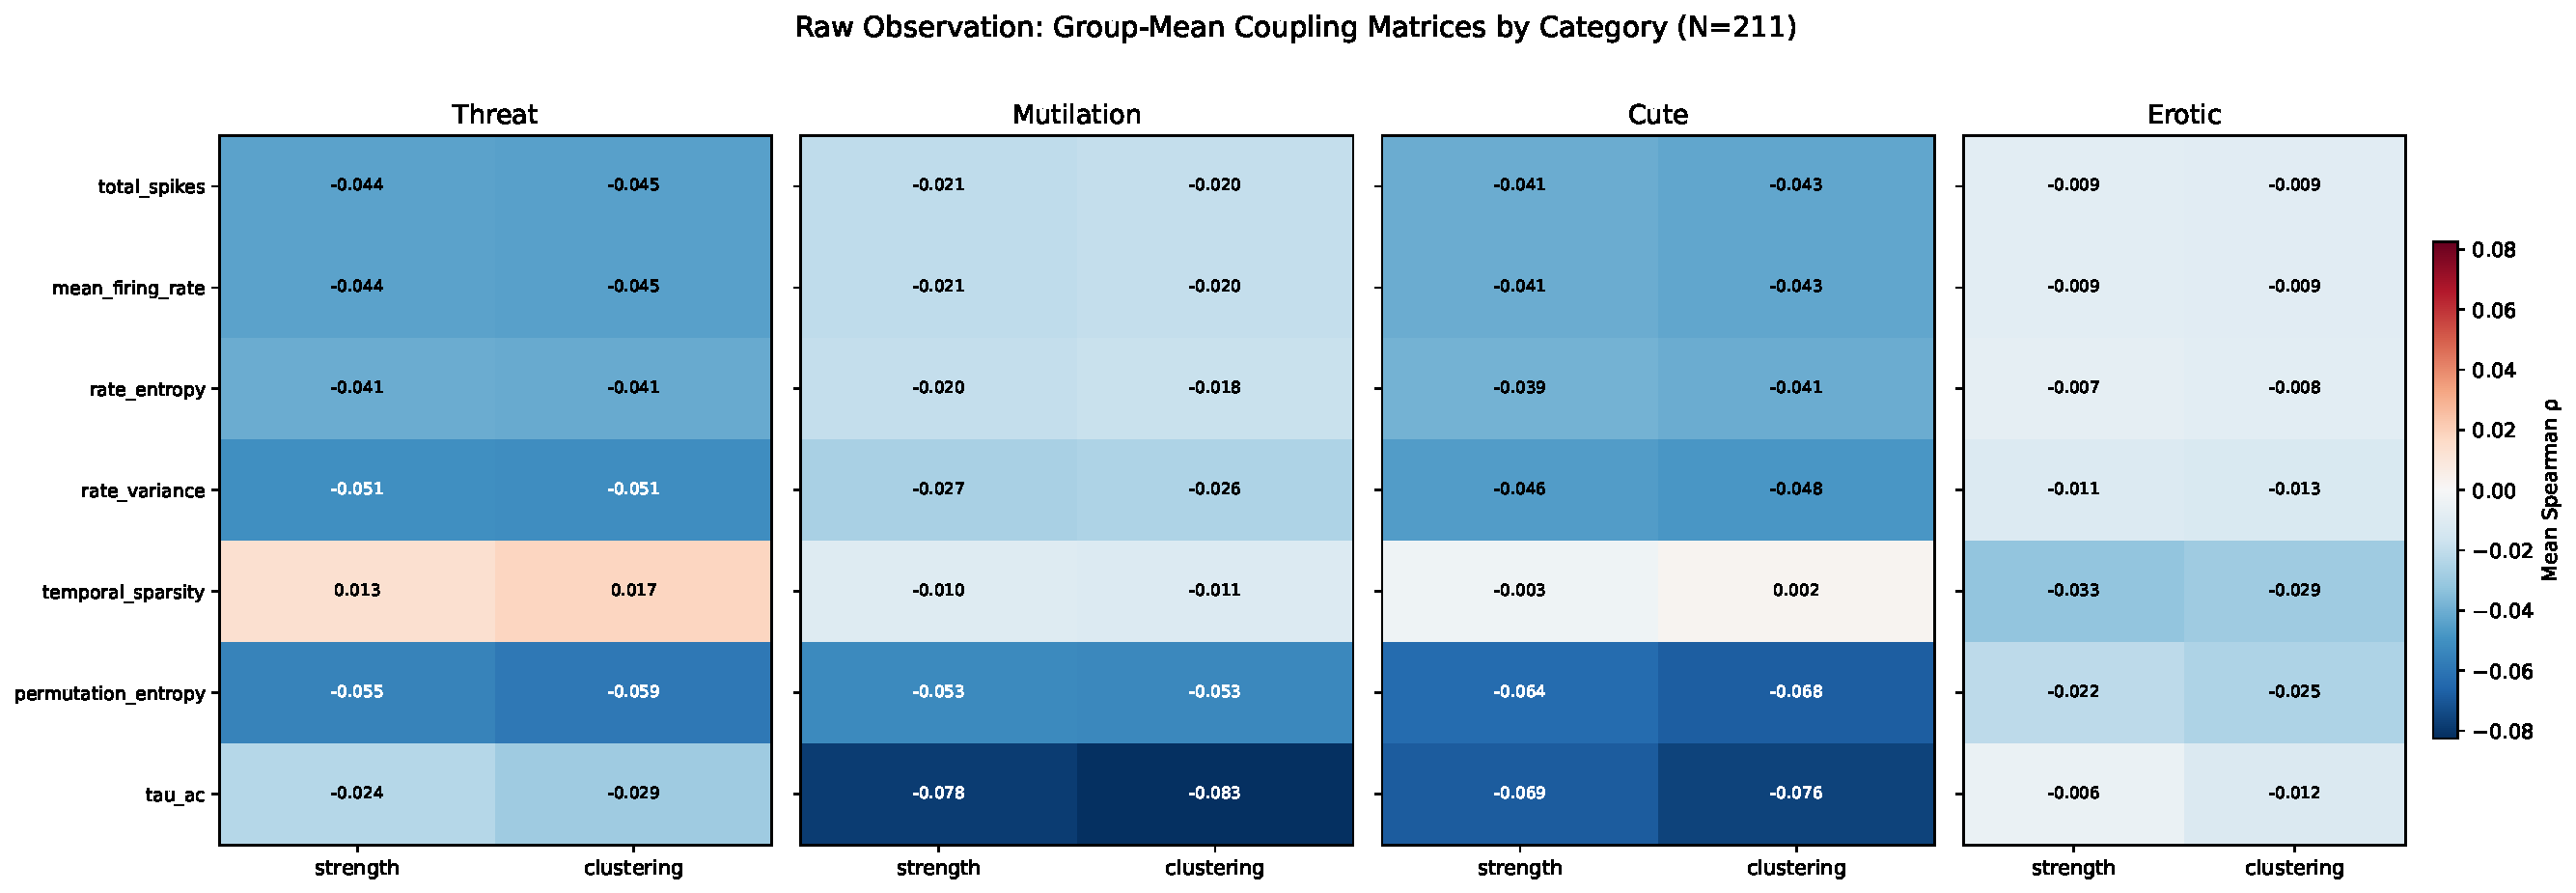
\includegraphics[width=0.95\textwidth]{pictures/chSynthesis/fig7_C1_category_C_matrices.pdf}
\caption{Group-mean coupling matrices by affective category ($N = 211$). Erotic shows the weakest coupling across all cells (most values near $-0.01$). Cute shows the strongest (permutation entropy $\times$ clustering $= -0.068$, $\tau_{AC} \times$ clustering $= -0.077$). Threat and Mutilation fall between, with different internal structures.}
\label{fig:category_C}
\end{figure}

In the sample means shown in Figure~\ref{fig:category_C}, most Erotic entries are near $-0.01$. The largest displayed Cute entries are permutation entropy $\times$ clustering at $-0.068$ and $\tau_{AC} \times$ clustering at $-0.077$. Threat and Mutilation have different sample patterns, including a Mutilation $\tau_{AC}$ correlation of $-0.083$.

\begin{figure}[htbp]
\centering
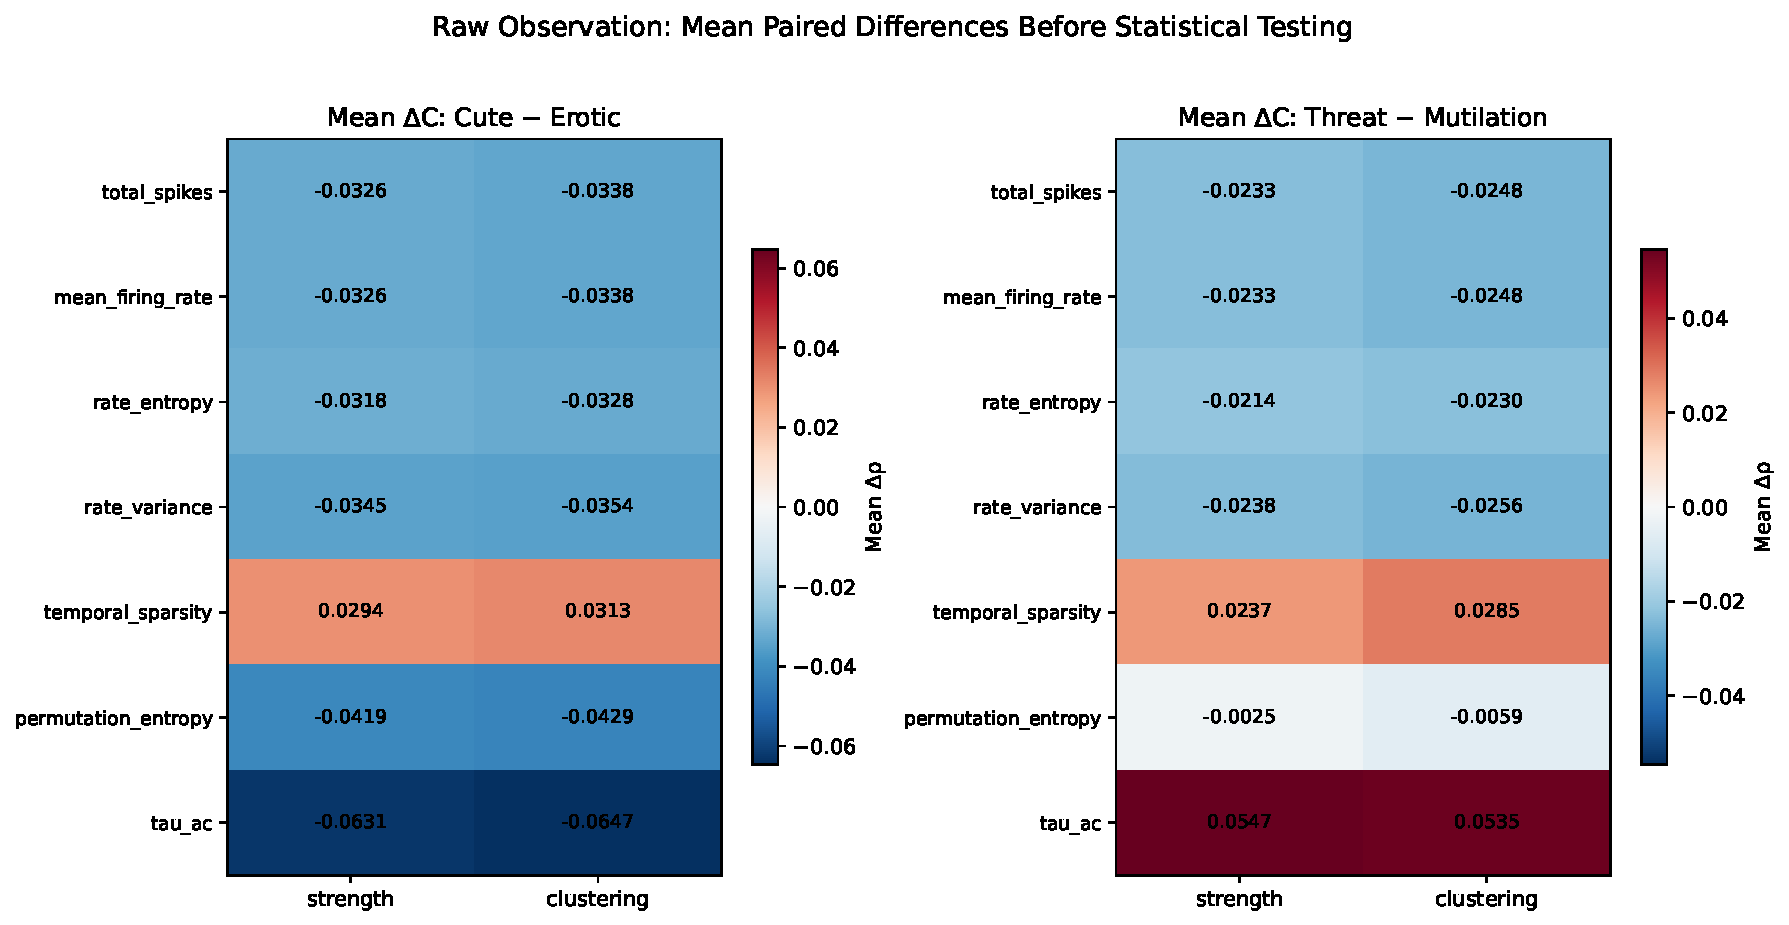
\includegraphics[width=0.95\textwidth]{pictures/chSynthesis/fig7_C2_raw_difference_matrices.pdf}
\caption{Mean paired difference matrices before statistical testing. Left: Cute $-$ Erotic shows consistent negative shifts (12 of 14 cells negative), with the largest differences in $\tau_{AC} \times$ clustering ($\Delta\rho = -0.065$) and $\tau_{AC} \times$ strength ($\Delta\rho = -0.063$). Right: Threat $-$ Mutilation shows a mixed pattern with $\tau_{AC}$ shifting in the opposite direction ($\Delta\rho = +0.054$).}
\label{fig:raw_diff_C}
\end{figure}

The raw Cute--Erotic paired differences (Figure~\ref{fig:raw_diff_C}) are negative in 12 of 14 cells, with only 43.1--46.9\% of subjects showing positive $\Delta\rho$ on the largest cells. The $\tau_{AC}$ row carries the largest shifts: $\Delta\rho = -0.065$ for $\tau_{AC} \times$ clustering and $-0.063$ for $\tau_{AC} \times$ strength.

\subsection{Quantitative Analysis}

\begin{figure}[htbp]
\centering
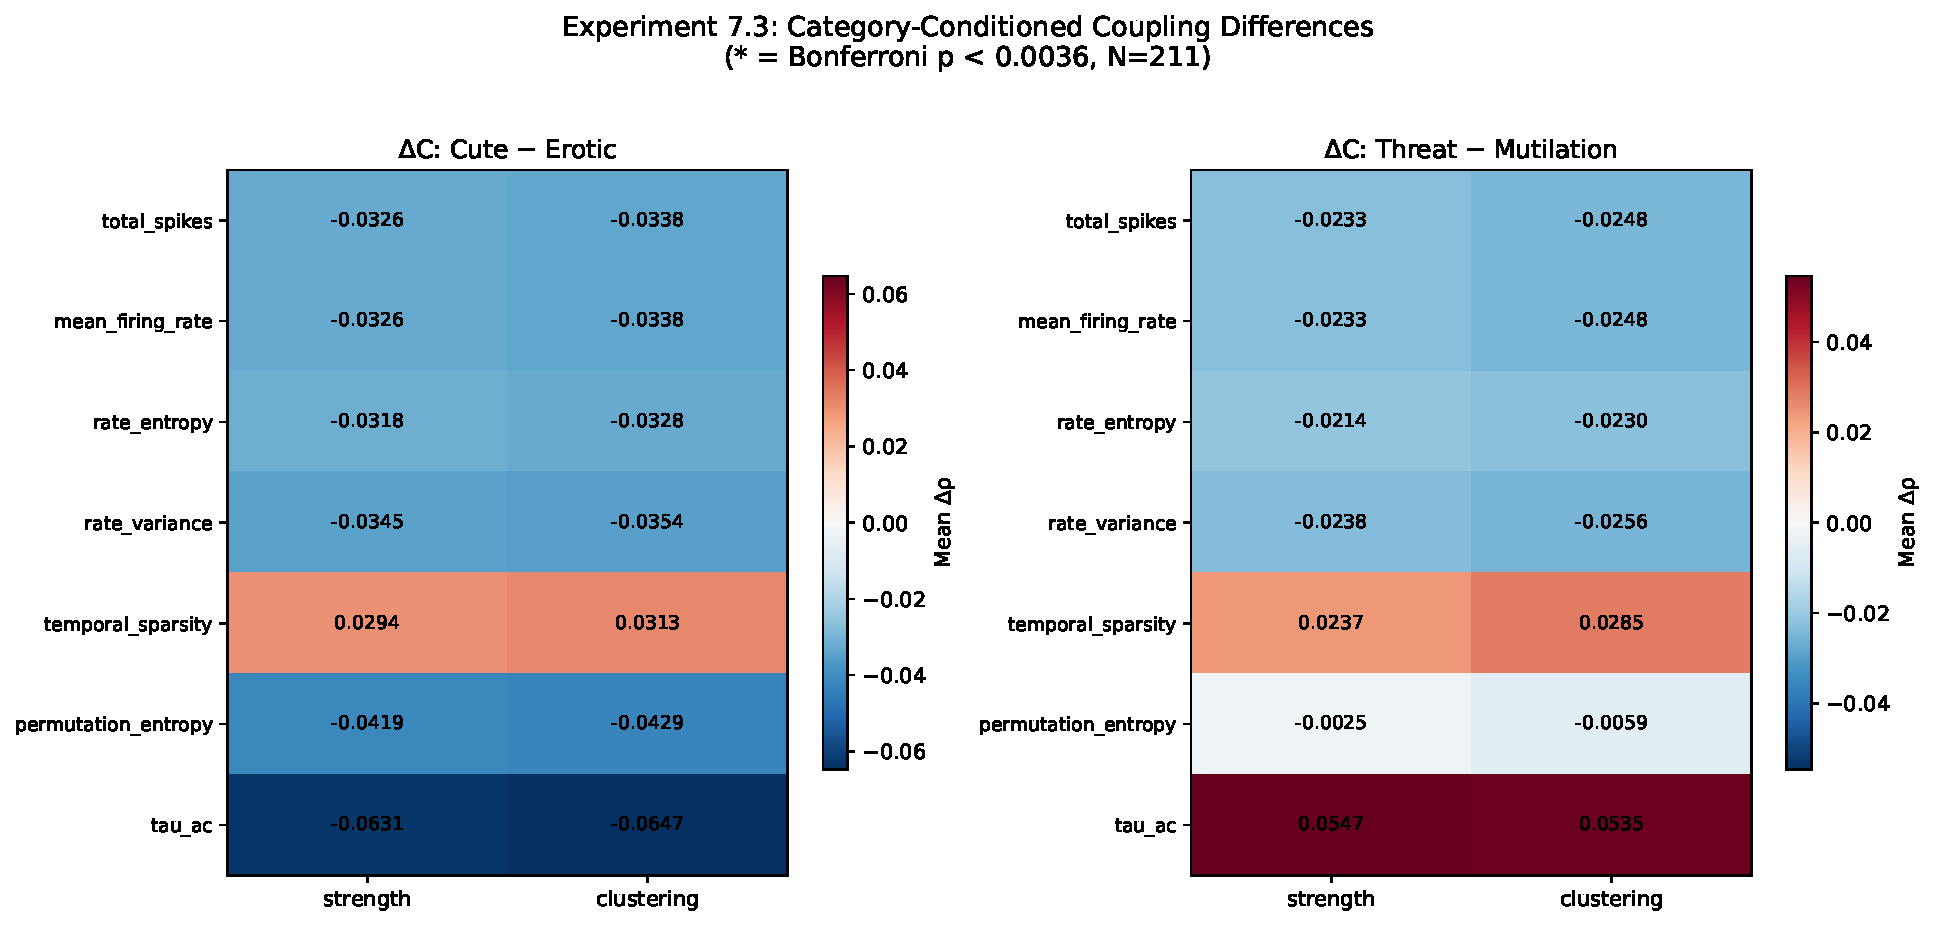
\includegraphics[width=0.95\textwidth]{pictures/chSynthesis/fig7_C3_difference_significance.pdf}
\caption{Difference matrices with Bonferroni significance masking ($\alpha = 0.05/14$). No individual cell reaches Bonferroni significance for either contrast. The $\tau_{AC}$ cells for Cute $-$ Erotic reach $p = 0.013$--$0.016$ uncorrected.}
\label{fig:diff_significance}
\end{figure}

No individual cell reaches Bonferroni significance for either within-valence contrast (0 of 14 for both; Figure~\ref{fig:diff_significance}). The closest are $\tau_{AC} \times$ clustering ($p = 0.013$, $d_z = 0.161$) and $\tau_{AC} \times$ strength ($p = 0.016$, $d_z = 0.155$) for Cute $-$ Erotic. The pattern-level Frobenius test is also non-significant (Cute $-$ Erotic: $\|\Delta\mathbf{C}\|_F = 0.150$, $p = 0.177$; Threat $-$ Mutilation: $\|\Delta\mathbf{C}\|_F = 0.109$, $p = 0.277$).

The temporal-structure group has the larger descriptive Cute--Erotic effect-size average (mean $|d_z| = 0.129$, minimum uncorrected $p = 0.013$), about $1.8\times$ the amplitude-associated group (mean $|d_z| = 0.072$, minimum uncorrected $p = 0.237$). This ratio was computed after grouping and inspecting the results and is not a confirmatory interaction test.

\subsection{Interpretation and Significance}

The Cute--Erotic sample difference is spread across 12 of 14 mean cells. However, no cell survives correction and the pattern-level Frobenius test is non-significant ($p=0.177$). The data therefore do not establish coordinated pattern-level modulation.

The largest uncorrected shifts occur for the two temporal-structure summaries. This is a hypothesis-generating rank ordering, not evidence of a distinct pathway or cross-chapter mechanism.

For Threat--Mutilation, the largest $\tau_{AC}$ comparison has $\Delta\rho=+0.054$ and uncorrected $p=0.024$. It does not survive the stated family correction and cannot establish content-specific reorganization.

A prospective replication should base sample size on an independently specified effect and analysis plan; a post-hoc calculation from the current selected cells is optimistic. The next section examines diagnosis-associated differences exploratorily.


\section{Experiment 7.4: Diagnosis-Group Comparisons}
\label{sec:exp7_diagnosis}

\subsection{Mathematical Motivation}

Earlier exploratory analyses reported diagnosis-associated descriptor differences. This section asks whether subject-mean coupling differs between one-versus-rest groups. The observable is $\Delta\bar{\kappa}=\bar{\kappa}_{\mathrm{Dx}^+}-\bar{\kappa}_{\mathrm{Dx}^-}$, where $\bar{\kappa}_s=\frac14\sum_c\kappa_{s,c}$.

All diagnosis comparisons are one-versus-rest within a transdiagnostic sample. The mean count is 2.0 among the five primary labels tested here; the broader supplied panel has mean 2.8. Results are diagnosis-associated coupling differences conditioned by that comorbidity structure, not disorder-specific signatures.

\subsection{Experimental Design}

Five diagnoses are tested: MDD ($n^+ = 142$, $n^- = 64$), SUD ($n^+ = 85$, $n^- = 121$), PTSD ($n^+ = 82$, $n^- = 124$), GAD ($n^+ = 60$, $n^- = 146$), and ADHD ($n^+ = 50$, $n^- = 156$). Group comparisons use Mann--Whitney~$U$ on $\bar{\kappa}_s$ with Bonferroni correction across five tests ($\alpha = 0.01$). A secondary analysis tests diagnosis $\times$ category interactions by permutation (5,000 iterations). Power analysis reports the minimum detectable Cohen's~$d$ at $\alpha = 0.05$, power $= 0.80$ for each comparison.

\subsection{Raw Observation}

\begin{figure}[htbp]
\centering
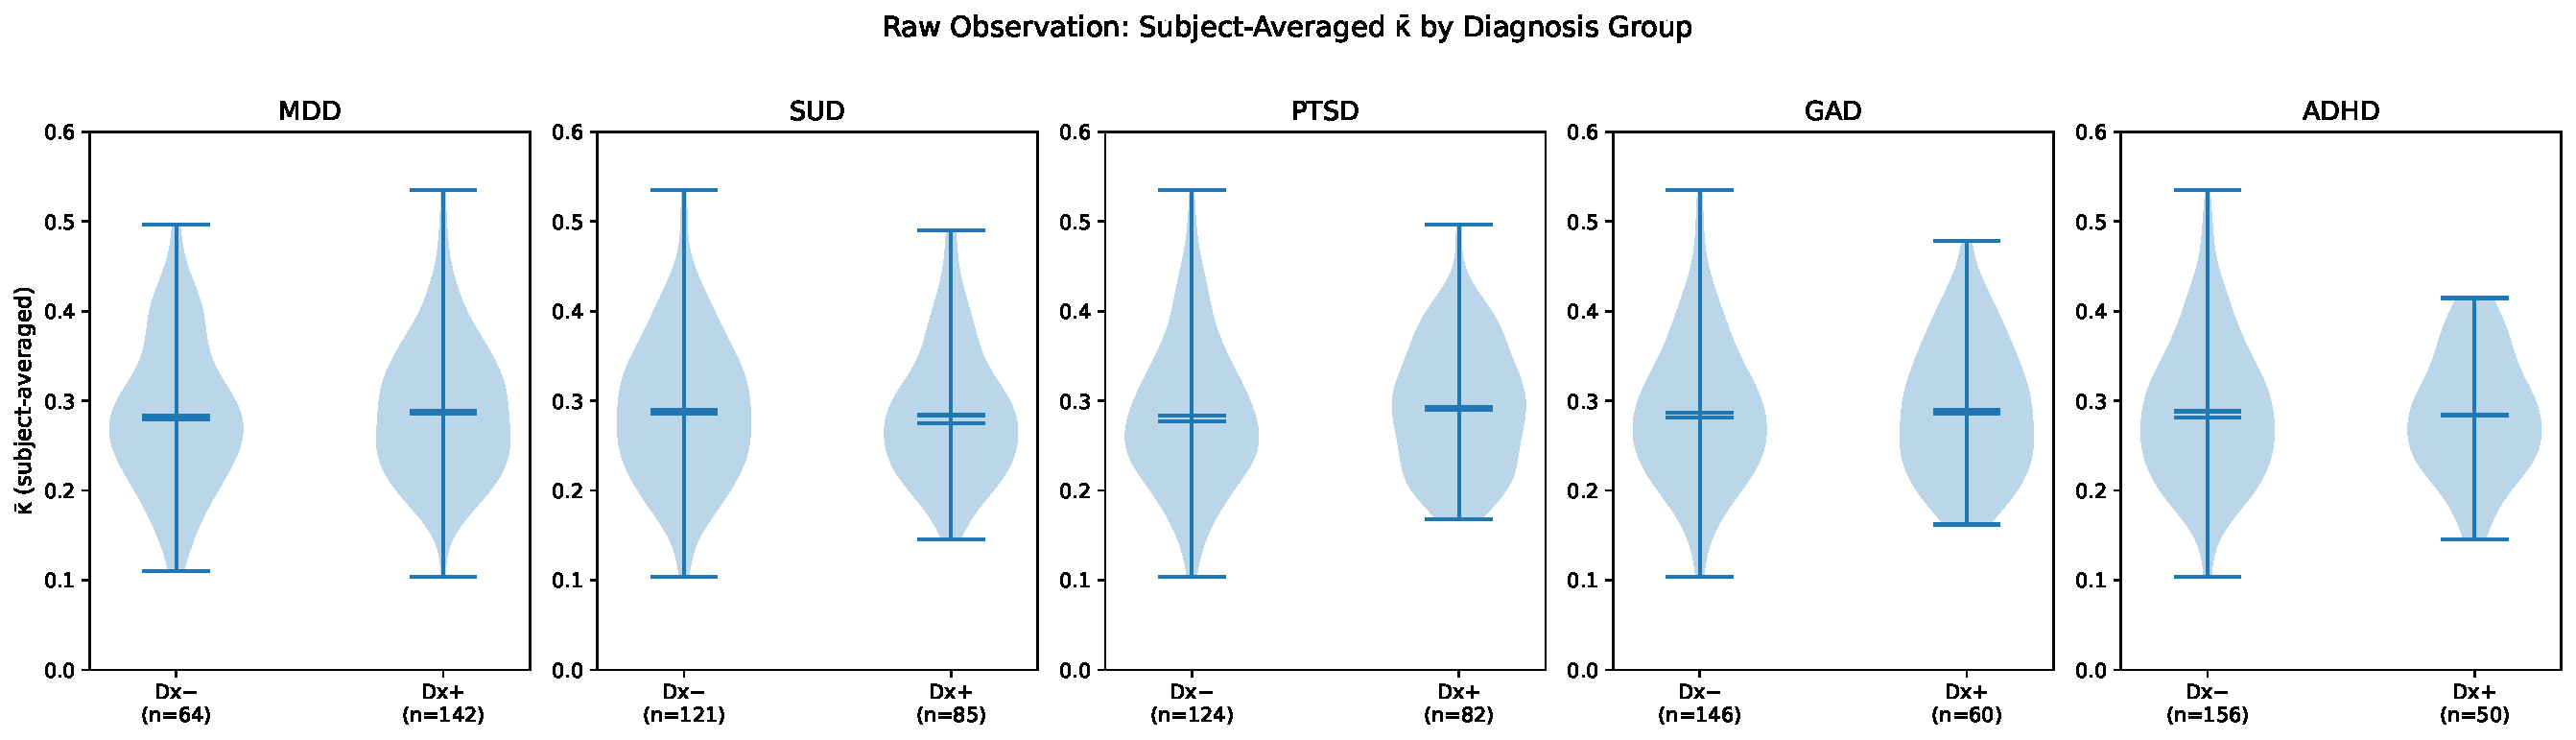
\includegraphics[width=0.95\textwidth]{pictures/chSynthesis/fig7_D1_raw_diagnosis_kappa.pdf}
\caption{Subject-averaged $\bar{\kappa}$ by diagnosis group for five diagnoses. The Dx$^+$ and Dx$^-$ distributions overlap extensively for all diagnoses. No visible separation is present in the raw violin plots.}
\label{fig:raw_diag_kappa}
\end{figure}

The raw violin plots (Figure~\ref{fig:raw_diag_kappa}) show near-complete distributional overlap between Dx$^+$ and Dx$^-$ for all five diagnoses. Group means differ by at most 0.009 (PTSD: $\bar{\kappa}_{\text{Dx}^+} = 0.293$ versus $\bar{\kappa}_{\text{Dx}^-} = 0.284$). The within-group standard deviations ($\approx 0.07$) are an order of magnitude larger than the between-group mean differences.

\subsection{Quantitative Analysis}

\begin{table}[htbp]
\centering
\caption{Diagnosis-associated coupling differences (Experiment~7.4).}
\label{tab:diagnosis_coupling}
\small
\begin{tabular}{lccccccc}
\toprule
\textbf{Dx} & \textbf{$n^+$} & \textbf{$n^-$} & \textbf{$\bar{\kappa}^+$} & \textbf{$\bar{\kappa}^-$} & \textbf{$d$} & \textbf{$p$} & \textbf{MDE} \\
\midrule
MDD & 142 & 64 & 0.289 & 0.283 & $+0.081$ & 0.609 & 0.42 \\
SUD & 85 & 121 & 0.284 & 0.290 & $-0.075$ & 0.485 & 0.40 \\
PTSD & 82 & 124 & 0.293 & 0.284 & $+0.116$ & 0.322 & 0.40 \\
GAD & 60 & 146 & 0.290 & 0.287 & $+0.043$ & 0.762 & 0.43 \\
ADHD & 50 & 156 & 0.285 & 0.288 & $-0.051$ & 0.921 & 0.46 \\
\bottomrule
\end{tabular}
\end{table}

No comparison reaches the five-test corrected threshold (Table~\ref{tab:diagnosis_coupling}); sample Cohen's~$d$ values are below 0.12. The reported minimum detectable effects of about 0.40--0.46 show that the study was not designed to exclude small differences. The result is therefore lack of evidence for a moderate or large scalar difference, not proof of absence.

\begin{figure}[htbp]
\centering
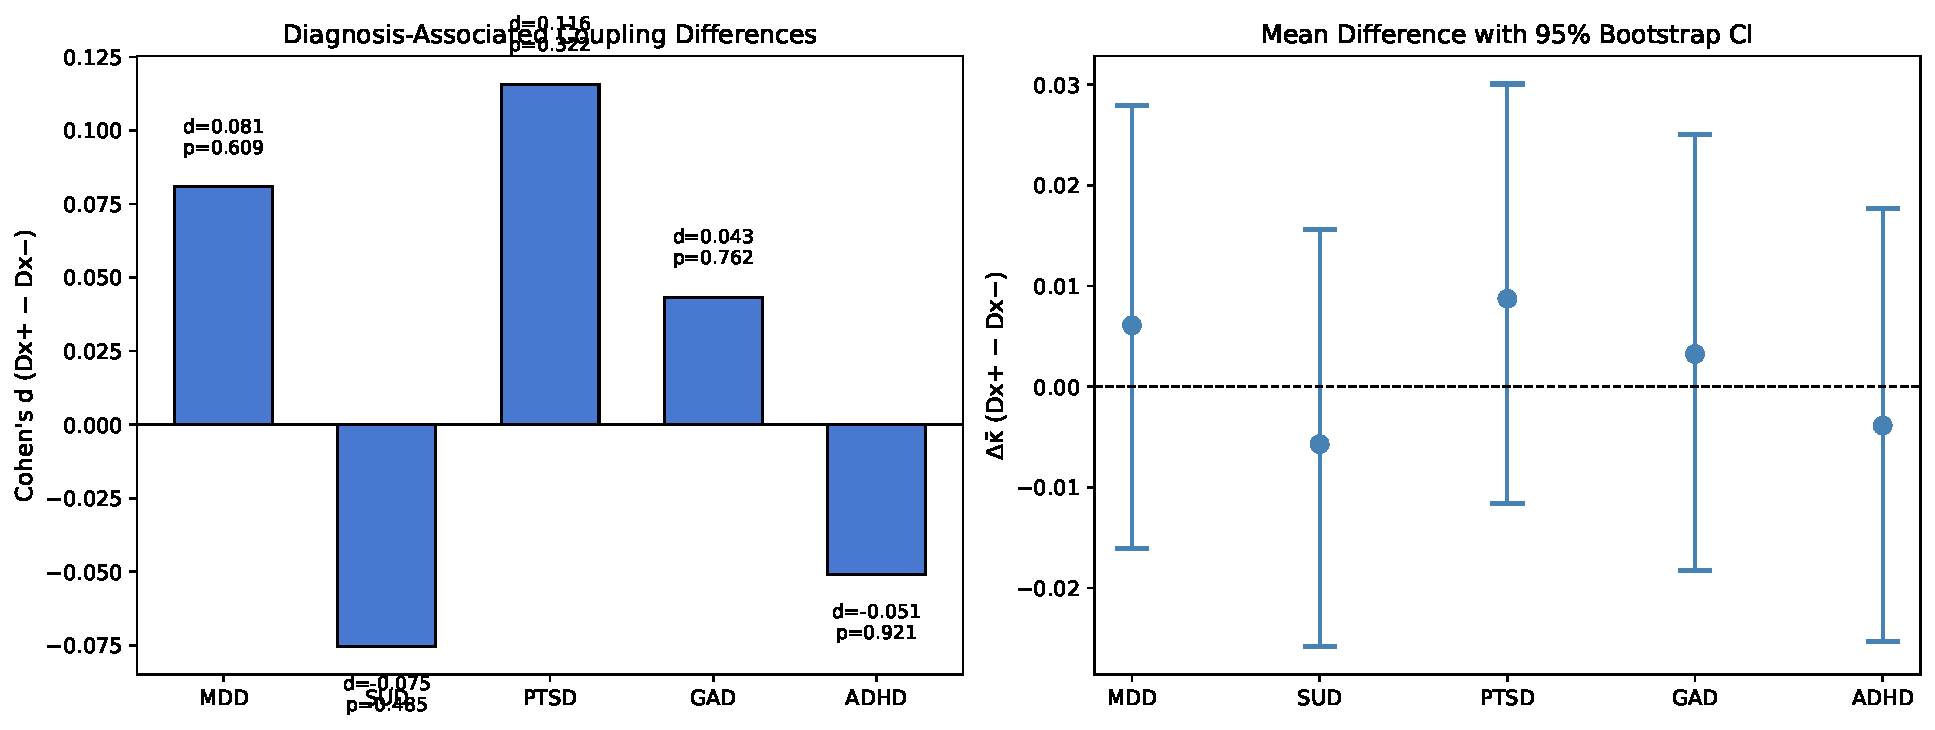
\includegraphics[width=0.95\textwidth]{pictures/chSynthesis/fig7_D2_diagnosis_effects.pdf}
\caption{Left: Cohen's~$d$ for each diagnosis. All values are below $|d| = 0.12$. Right: bootstrap 95\% confidence intervals for the mean $\bar{\kappa}$ difference. All intervals include zero.}
\label{fig:diagnosis_effects}
\end{figure}

The secondary diagnosis $\times$ category interaction analysis identifies one suggestive pattern: ADHD shows a category-dependent coupling profile with the lowest $\kappa$ for Mutilation (0.261) and the highest for Erotic (0.308), reaching $p = 0.035$ uncorrected. This does not survive Bonferroni correction across five diagnoses and is carried forward as a hypothesis for future investigation.

\subsection{Interpretation and Significance}

Within this one-versus-rest, comorbid sample, subject-mean $\kappa$ does not show corrected diagnosis-group separation. This does not demonstrate equivalence, and it should not be used to infer that the individual descriptor families contain disorder-specific effects.

The ADHD interaction has uncorrected $p=0.035$ and does not survive the five-diagnosis correction. It is retained only as a hypothesis.

A natural question follows: if coupling is organizationally informative but not diagnosis-discriminative at the scalar level, do the individual descriptor families carry complementary discriminative information when combined?


\section{Experiment 7.5: Augmentation Ablation}
\label{sec:exp7_augmentation}

\subsection{Mathematical Motivation}

The final four-category analysis compares linear-readout AUC for topology, dynamics, their concatenation, and concatenation plus $\kappa$. It is an exploratory model comparison, not a test of clinical detection utility.

\subsection{Experimental Design}

Four feature conditions are constructed from subject-averaged per-electrode descriptors: T-only (68 features: 34 electrodes $\times$ 2 topology metrics), D-only (238 features: 34 electrodes $\times$ 7 dynamical metrics), T+D (306 features: concatenation), and T+D+$\kappa$ (307 features: concatenation plus subject-averaged coupling strength). Five binary detection tasks are tested: SUD, MDD, PTSD, GAD, and ADHD. The primary readout is $L_2$-regularized logistic regression ($C = 1.0$) with subject-level stratified 5-fold cross-validation repeated 10 times (50 total folds).

\subsection{Raw Observation}

\begin{figure}[htbp]
\centering
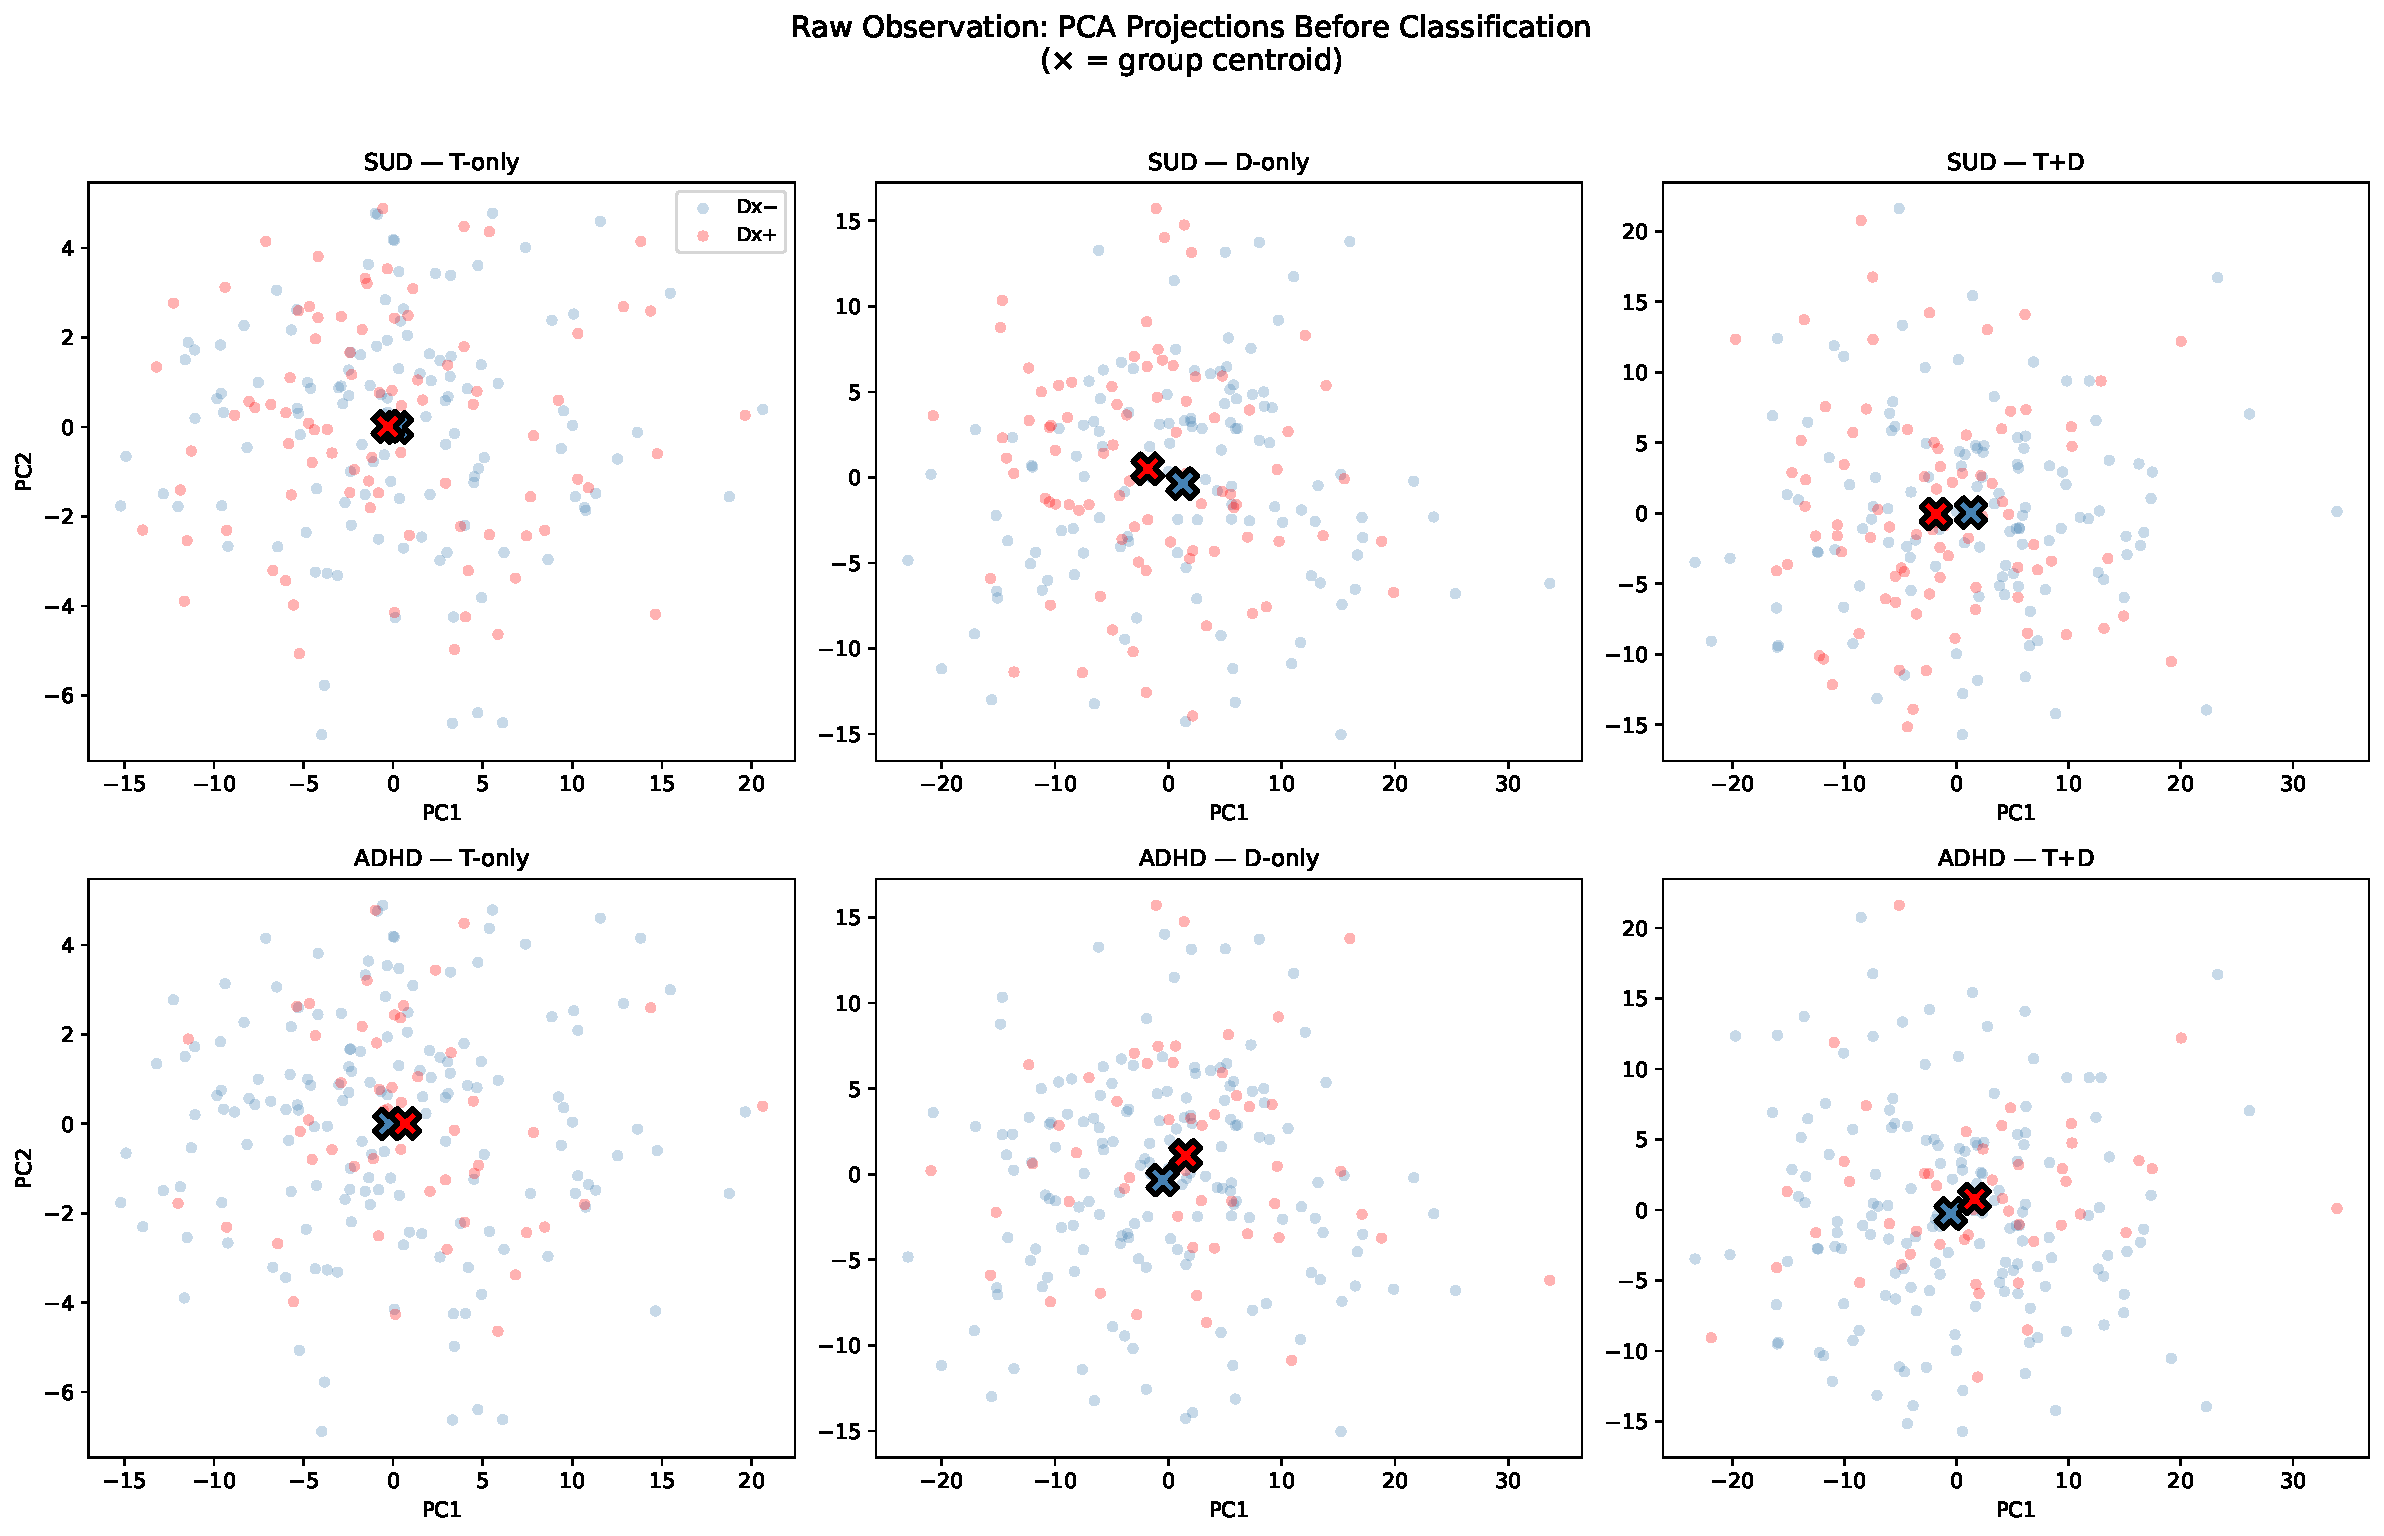
\includegraphics[width=0.95\textwidth]{pictures/chSynthesis/fig7_E1_raw_pca_projections.pdf}
\caption{PCA projections before classification for SUD (top) and ADHD (bottom) across T-only, D-only, and T+D feature spaces. Group centroids ($\times$) are marked. SUD shows near-complete overlap in all three spaces. ADHD shows visible D-only centroid offset that is absent in T-only.}
\label{fig:pca_projections}
\end{figure}

The dynamics and concatenated matrices have more columns than independent subjects and are rank-deficient. Full-sample PCA plots are visualization only and cannot predict held-out performance. The counts of univariate $p<0.05$ are uncorrected screens across hundreds of features and are not evidence of localized effects.

\begin{figure}[htbp]
\centering
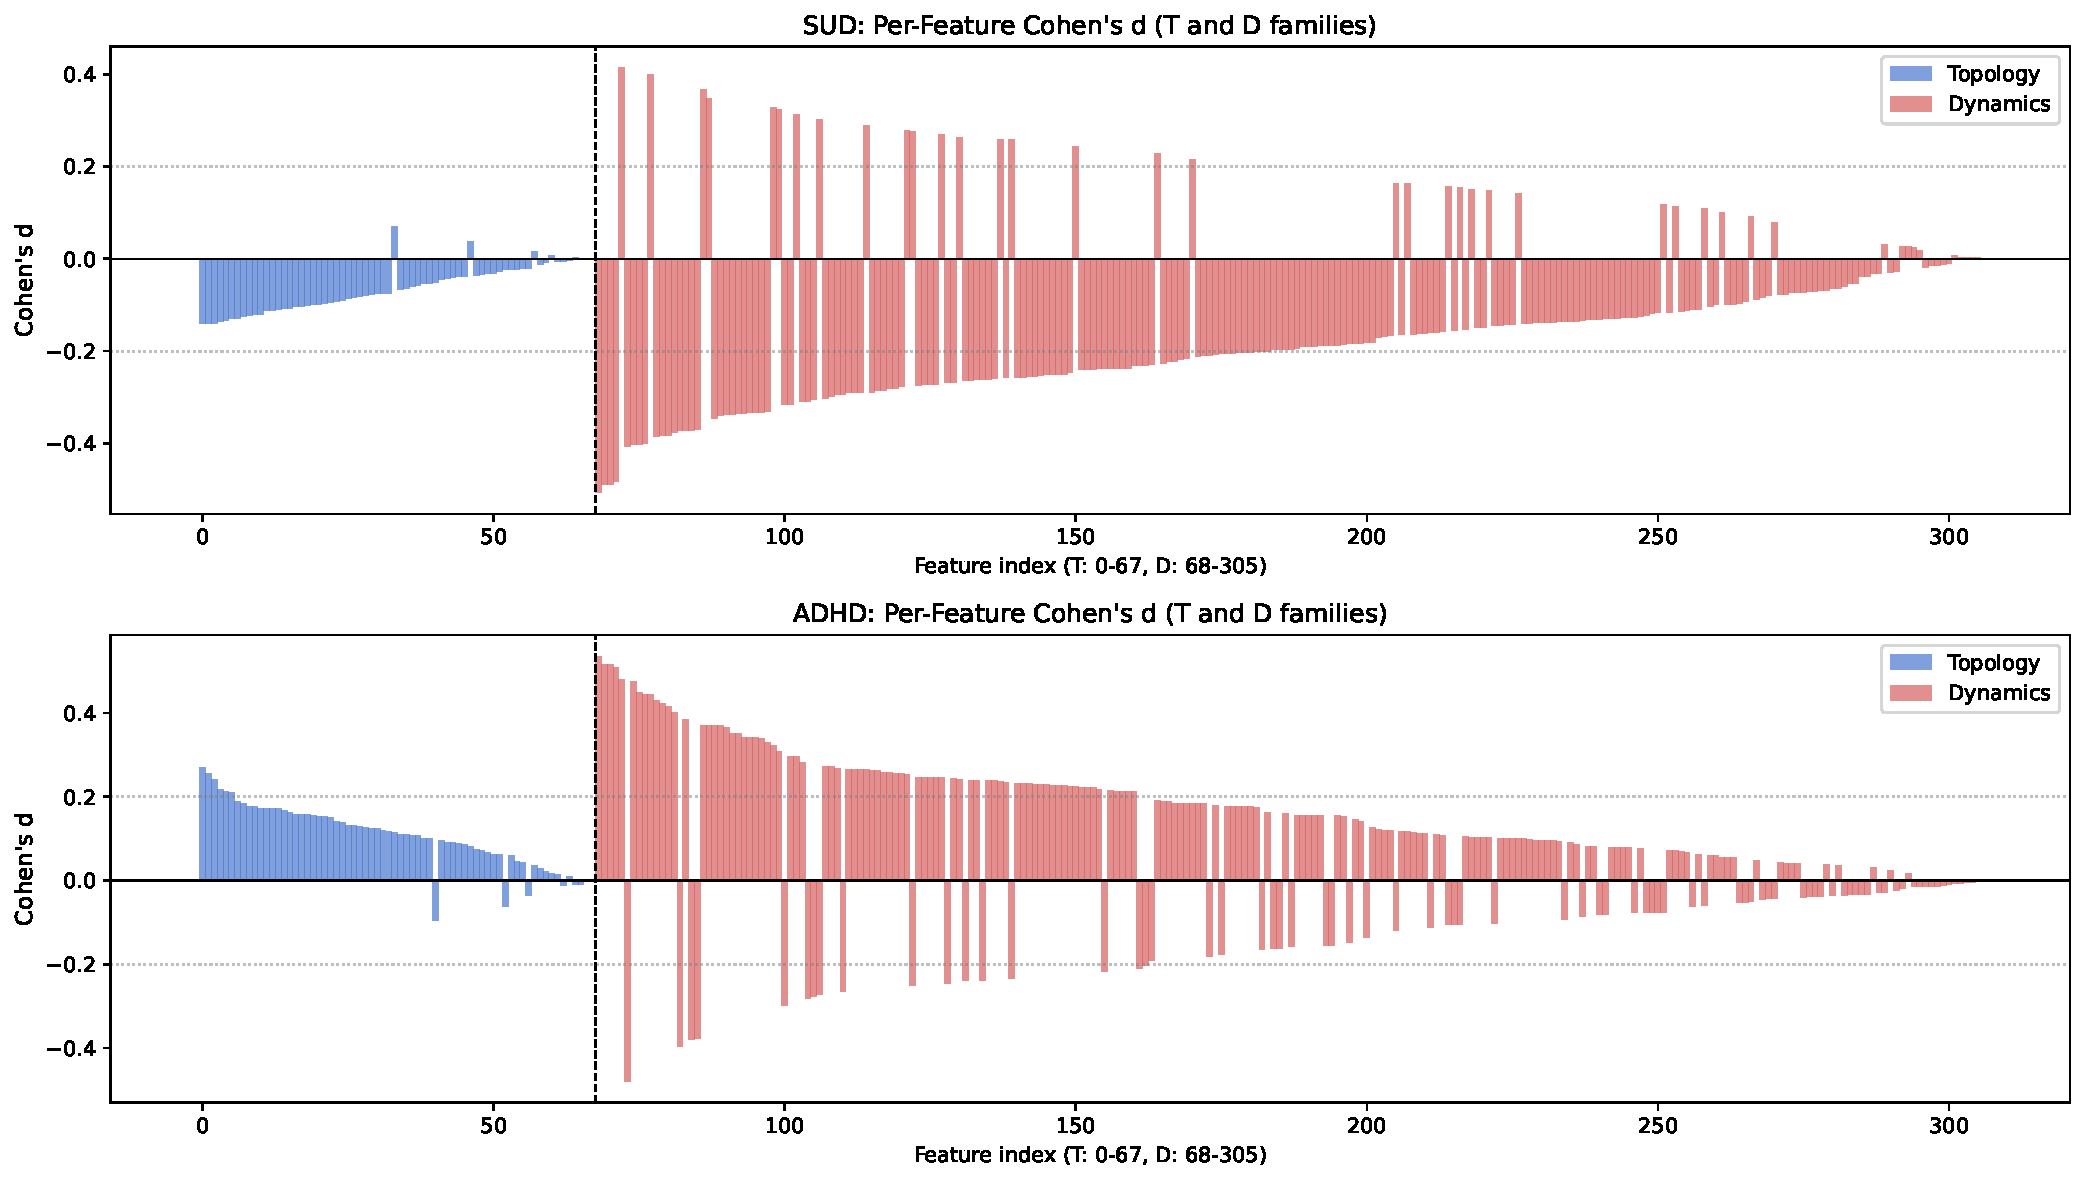
\includegraphics[width=0.95\textwidth]{pictures/chSynthesis/fig7_E2_raw_univariate_effects.pdf}
\caption{Per-feature Cohen's~$d$ across all 306 features for SUD (top) and ADHD (bottom). Topology features (left of vertical line) cluster near $d = 0$. Dynamics features (right) show scattered effects, broader for ADHD than SUD.}
\label{fig:univariate_effects}
\end{figure}

These plots motivated, but did not preregister or guarantee, the subsequent classifier comparison.

\subsection{Quantitative Analysis}

\begin{table}[htbp]
\centering
\caption{Augmentation comparison: mean AUC and standard deviation across 50 overlapping repeated-CV folds. Fold standard deviations are not confidence intervals.}
\label{tab:augmentation}
\small
\begin{tabular}{lcccc}
\toprule
\textbf{Dx} & \textbf{T-only} & \textbf{D-only} & \textbf{T+D} & \textbf{T+D+$\kappa$} \\
\midrule
SUD & $0.464 \pm 0.071$ & $0.464 \pm 0.076$ & $0.458 \pm 0.083$ & $0.455 \pm 0.082$ \\
MDD & $0.518 \pm 0.094$ & $0.504 \pm 0.085$ & $0.512 \pm 0.092$ & $0.510 \pm 0.090$ \\
PTSD & $0.487 \pm 0.072$ & $0.527 \pm 0.073$ & $0.510 \pm 0.069$ & $0.505 \pm 0.069$ \\
GAD & $\mathbf{0.581} \pm 0.092$ & $0.533 \pm 0.093$ & $0.568 \pm 0.084$ & $0.563 \pm 0.083$ \\
ADHD & $0.533 \pm 0.077$ & $\mathbf{0.622} \pm 0.086$ & $0.597 \pm 0.076$ & $0.608 \pm 0.084$ \\
\bottomrule
\end{tabular}
\end{table}

In the recorded repeated splits, SUD AUC is about 0.46 across conditions; the largest mean is 0.622 for ADHD with dynamics, and the largest GAD mean is 0.581 with topology. Concatenation does not exceed the better single family for any of the five labels in this finite comparison.

\begin{figure}[htbp]
\centering
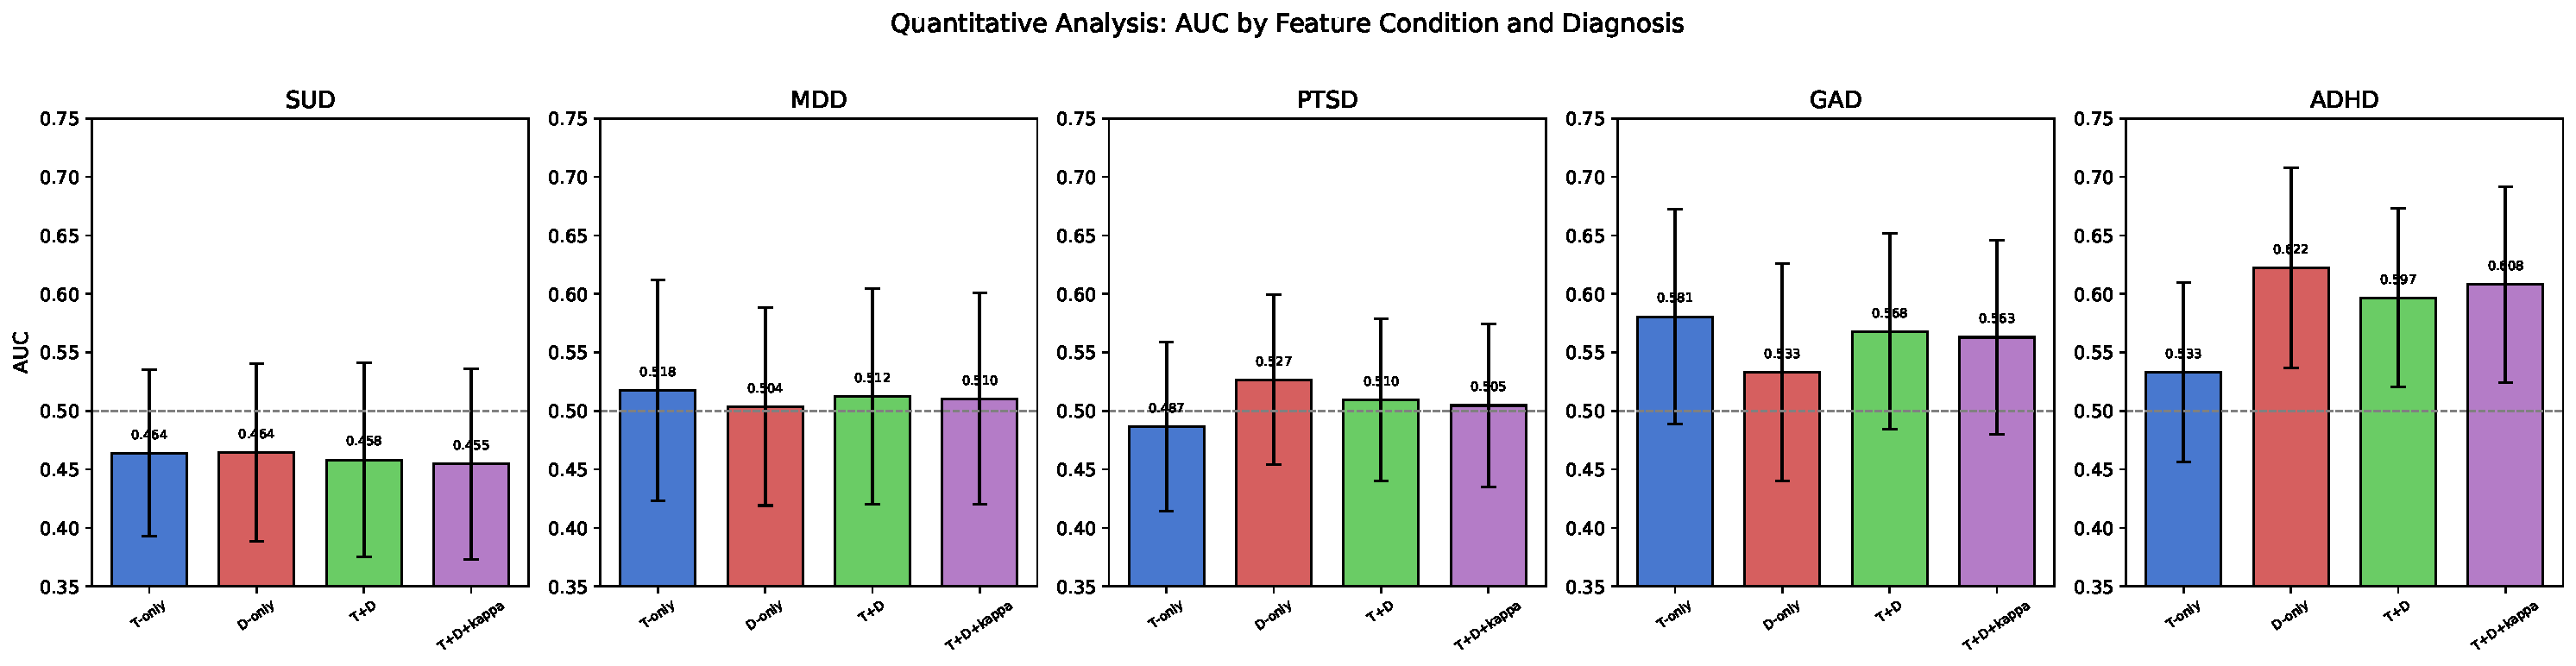
\includegraphics[width=0.95\textwidth]{pictures/chSynthesis/fig7_E4_classification_auc.pdf}
\caption{Mean repeated-CV AUC by feature condition and diagnosis. Bold values mark the largest sample mean per diagnosis; they are not multiplicity-adjusted claims of above-chance clinical performance.}
\label{fig:classification_auc}
\end{figure}

For ADHD, the recorded mean changes from 0.622 (D-only) to 0.597 (T+D) and 0.608 (T+D+$\kappa$). The archived $p$-values treated 50 overlapping fold scores as independent and are invalid; they are not used. These small mean differences do not establish non-redundant ADHD information.

\subsection{Interpretation and Significance}

The narrow conclusion is that concatenation did not improve the sample mean AUC in these models and splits. That does not prove the feature families lack complementary information under other estimators or cohorts.

The per-diagnosis maxima are post-hoc model-selection observations. They do not show diagnosis specificity or support a complete clinical characterization.

The ADHD interaction and augmentation observations arise from the same cohort and are not independent replications. One is uncorrected and the other relied on invalid fold-level inference. They are retained only as exploratory prompts for a prespecified external study.


\section{Separate Three-Condition Analysis}
\label{sec:ch7_3class}

This section reports a separate Negative/Neutral/Pleasant pipeline. It is not a replication of the four-category analysis because the observations, preprocessing, and archived reservoir update differ. Archived PCA-based condition-variance ratios are also affected by global PCA fitting and do not imply tighter confidence intervals. The comparison below is therefore a cross-pipeline sensitivity analysis.

\subsection{Coupling Existence at Three-Class}

The mean coupling scalar is $\kappa=0.221\pm0.111$. None of 5,000 permuted means equaled or exceeded the observed mean. With the standard plus-one Monte Carlo correction, the result is $p=1/5001\approx0.0002$, not zero. The corrected script uses this calculation; the archived figure's displayed zero was generated before the audit.

Six of the 14 sample-mean entries are negative and eight positive. Their signs and magnitudes describe cross-channel association in this pipeline; they do not show that connectivity produces a particular reservoir response. The contrast with the four-category sign pattern is confounded by the different archived implementations.

\begin{figure}[H]
    \centering
    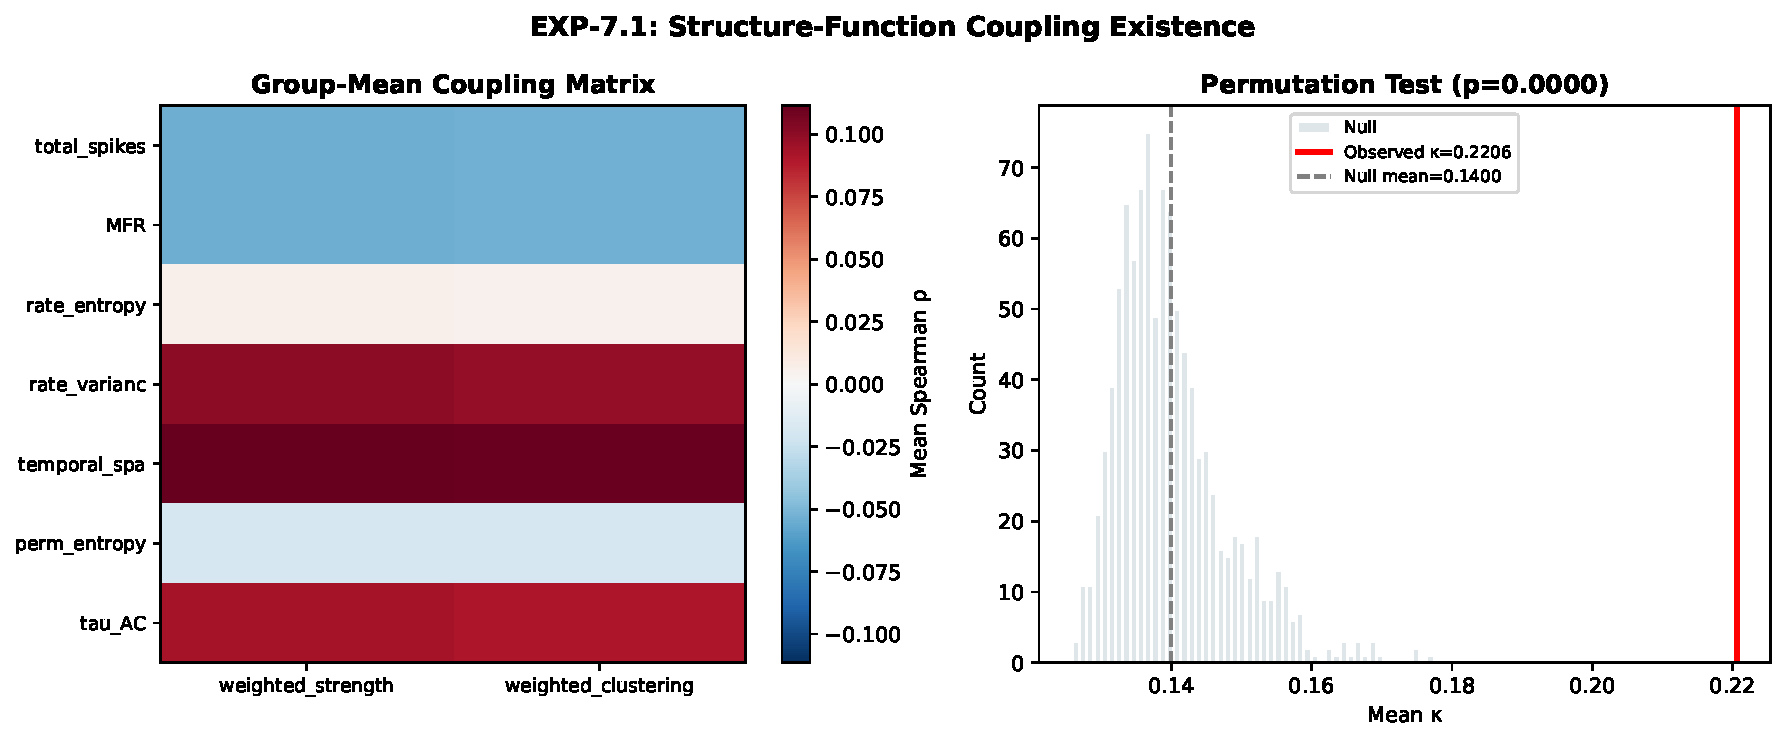
\includegraphics[width=\textwidth]{pictures/chSynthesis/fig_3class_coupling_existence.pdf}
    \caption{Three-condition coupling summary ($N=211$, 633 observations). The mean matrix has six negative and eight positive entries. The archived plot labels the 5,000-permutation result as zero; the corrected plus-one Monte Carlo value is $p=1/5001\approx0.0002$.}
    \label{fig:ch7_3class_coupling}
\end{figure}

\subsection{Variance Decomposition at Three-Class}

The sample sums-of-squares fractions are 40.3\% subject, 0.7\% condition, and 59.0\% residual (Figure~\ref{fig:ch7_3class_variance}); the condition test gives $F=2.33$, $p=0.101$. A non-significant $p$-value is not a trend, and the differing fractions cannot be attributed to condition strength because the two pipelines are not matched.

\begin{figure}[H]
    \centering
    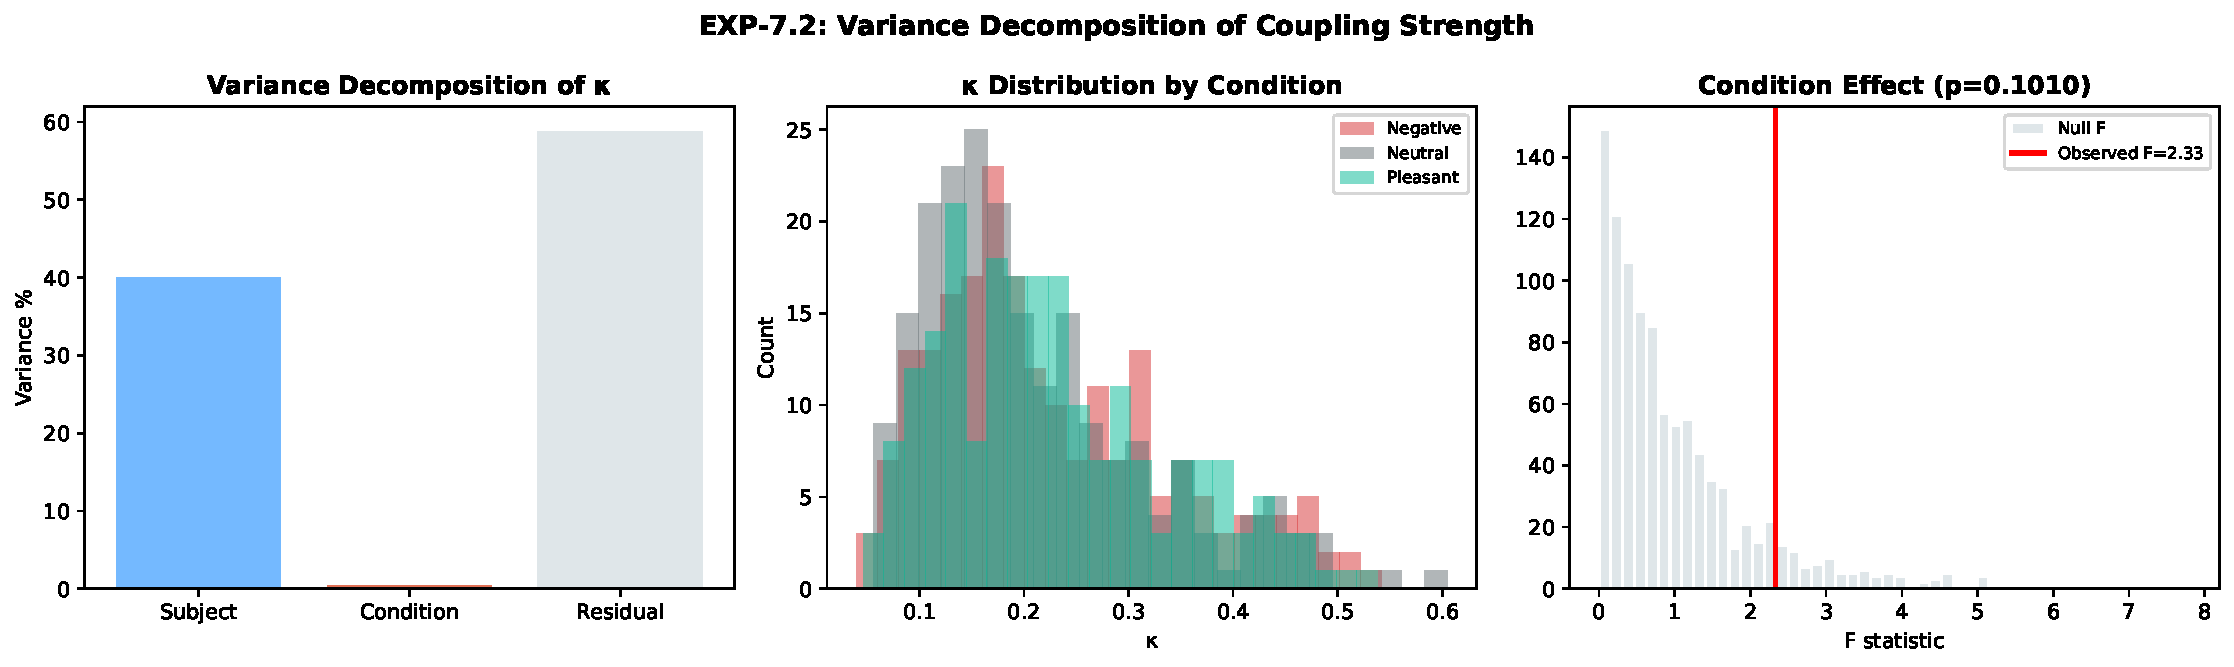
\includegraphics[width=\textwidth]{pictures/chSynthesis/fig_3class_variance_decomposition.pdf}
    \caption{Three-condition sample sums-of-squares decomposition: subject 40.3\%, condition 0.7\%, residual 59.0\%; condition permutation $p=0.101$. Fractions are descriptive and are not directly comparable with the unmatched four-category pipeline.}
    \label{fig:ch7_3class_variance}
\end{figure}

\subsection{Clinical Coupling at Three-Class}

No tested group comparison has $p<0.39$ in the three-condition analysis (Figure~\ref{fig:ch7_3class_clinical}); sample $d$ ranges from $-0.175$ to $+0.099$. This is lack of detected separation, not equivalence or evidence about independent clinical utility.

\begin{figure}[H]
    \centering
    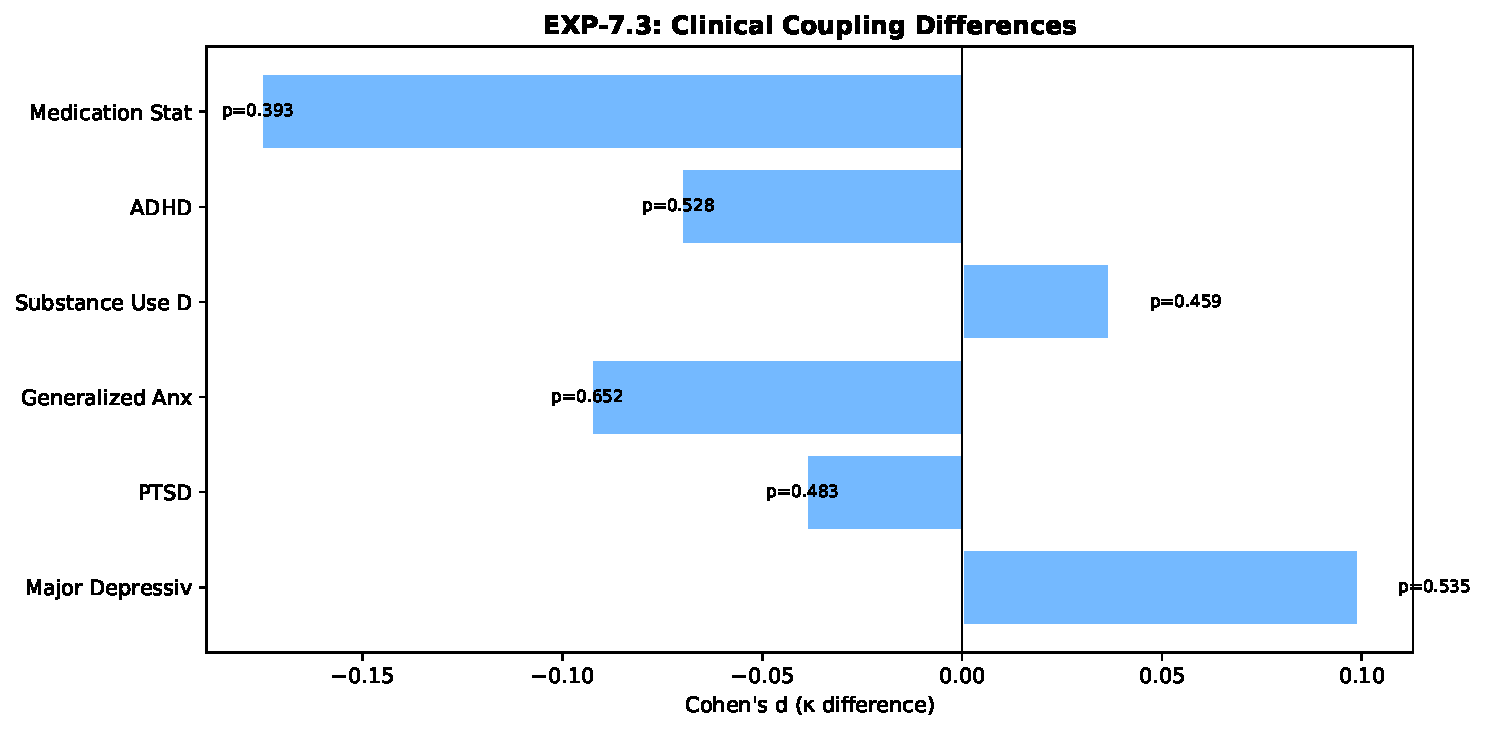
\includegraphics[width=0.85\textwidth]{pictures/chSynthesis/fig_3class_clinical_coupling.pdf}
    \caption{Three-condition coupling group comparisons for six clinical variables. No reported comparison has $p<0.39$; this does not establish equivalence.}
    \label{fig:ch7_3class_clinical}
\end{figure}

\subsection{Condition-Conditioned Coupling Structure at Three-Class}

The Frobenius norm test for pattern-level Negative--Pleasant differences in the coupling matrix produces $p = 0.376$, and zero of $14$ individual cells reach Bonferroni significance (Figure~\ref{fig:ch7_3class_condition}). The analysis therefore provides no evidence of a Negative--Pleasant pattern difference under the stated tests.

The Negative--Pleasant Frobenius test is non-significant, and the four-category Cute--Erotic scalar comparison is nominal and uncorrected while its pattern test is also non-significant. These results do not show that reorganization requires finer affective distinctions.

\begin{figure}[H]
    \centering
    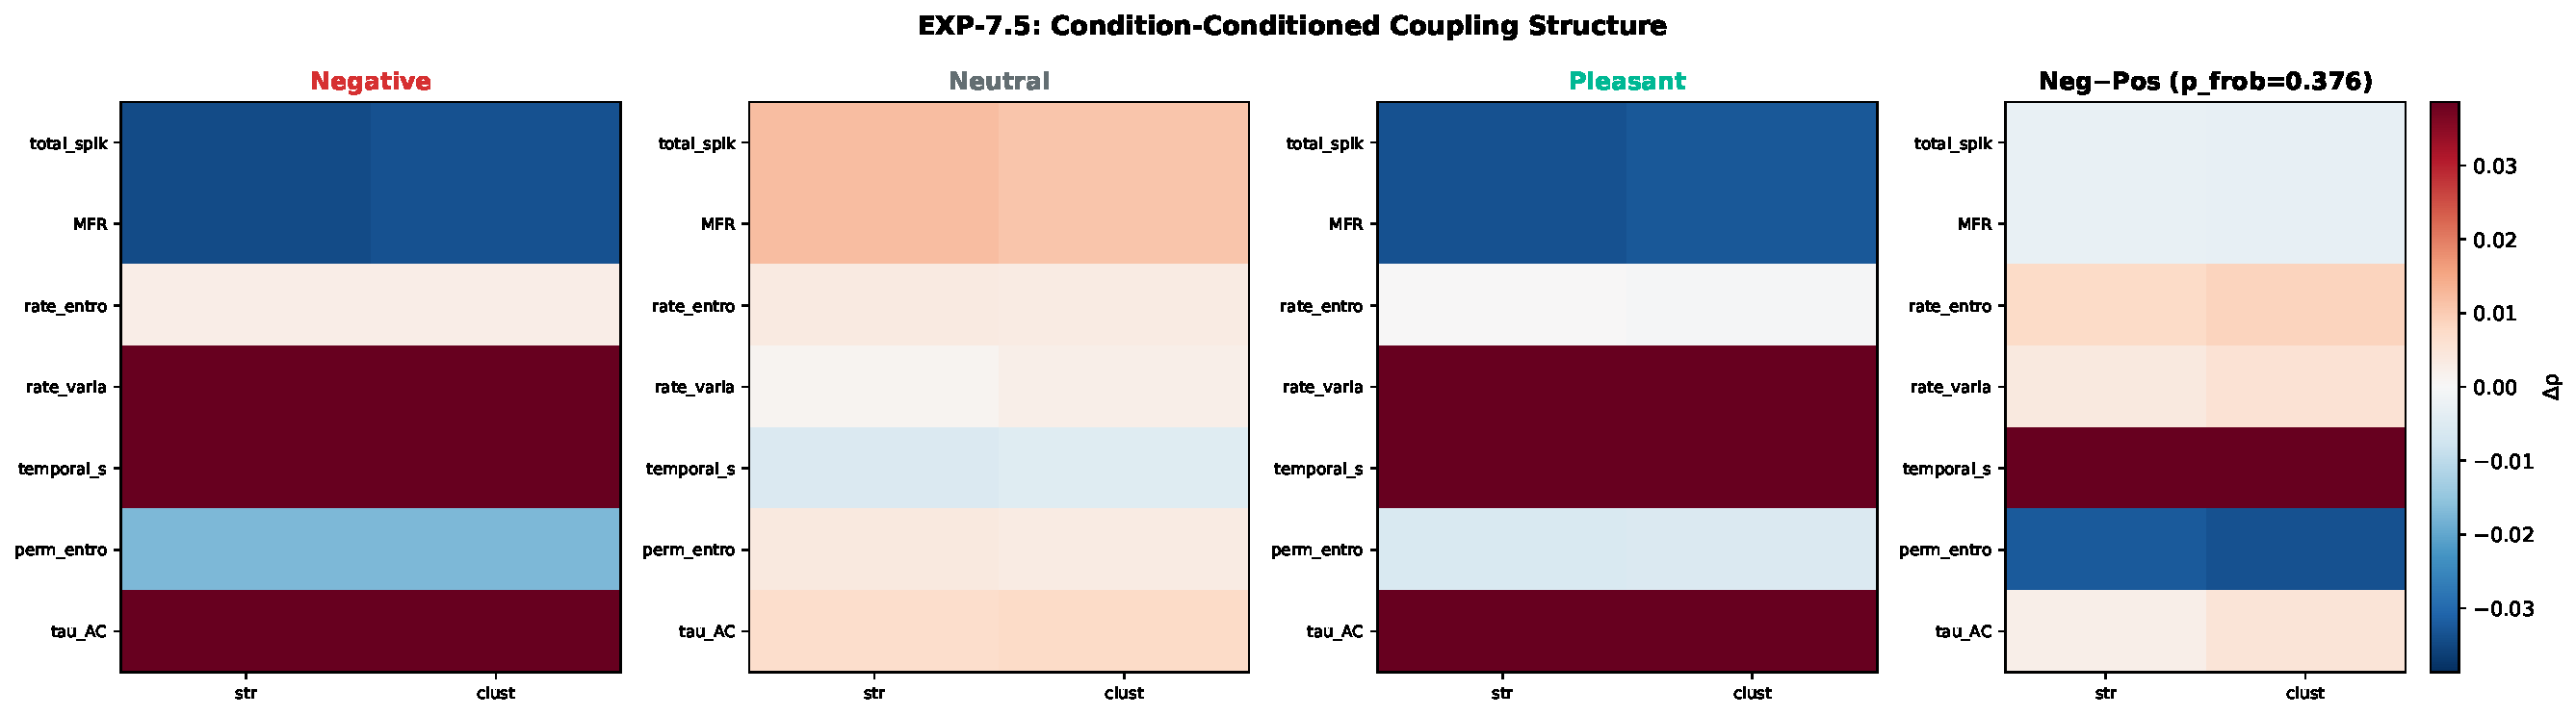
\includegraphics[width=\textwidth]{pictures/chSynthesis/fig_3class_condition_coupling.pdf}
    \caption{Three-condition coupling matrices and Negative--Pleasant difference matrix; the Frobenius sign-flip test gives $p=0.376$, with zero of 14 cells surviving Bonferroni correction.}
    \label{fig:ch7_3class_condition}
\end{figure}

\subsection{Augmentation Ablation at Three-Class}

In one fixed five-fold split, combined features do not exceed the better single family for the tested labels (Figure~\ref{fig:ch7_3class_augmentation}); balanced accuracies range from 43\% to 53\%. The invalid four-category fold-level $p$-value is not used, and the unmatched pipelines do not support a replication claim.

\begin{figure}[H]
    \centering
    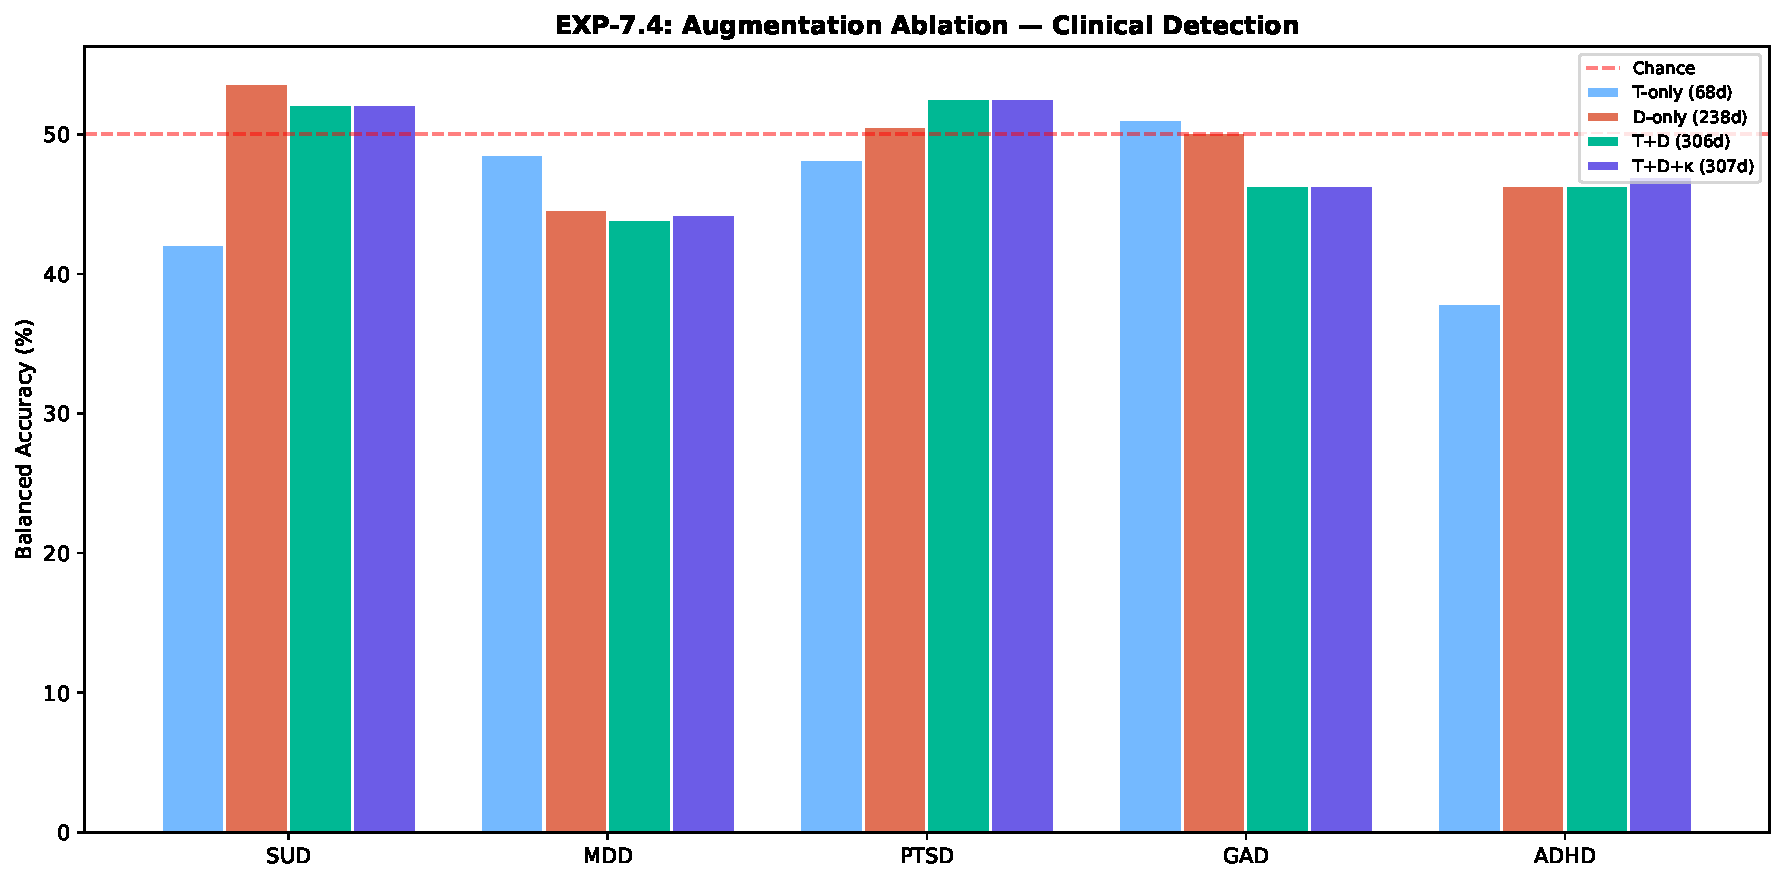
\includegraphics[width=0.85\textwidth]{pictures/chSynthesis/fig_3class_augmentation.pdf}
    \caption{Three-condition, fixed five-fold balanced accuracy for topology, dynamics, their concatenation, and concatenation plus $\kappa$. The finite comparison does not establish absence of complementary information.}
    \label{fig:ch7_3class_augmentation}
\end{figure}

\subsection{Cross-Granularity Summary}

Table~\ref{tab:ch7_cross_granularity} summarizes the coupling results across both granularities.

\begin{table}[H]
\centering
\caption{Descriptive comparison of unmatched three-condition and four-category pipelines.}
\label{tab:ch7_cross_granularity}
\footnotesize
\begin{tabularx}{\textwidth}{>{\raggedright\arraybackslash}p{3.2cm}>{\raggedright\arraybackslash}X>{\raggedright\arraybackslash}X}
\hline
\textbf{Property} & \textbf{3-class} & \textbf{4-class} \\
\hline
Mean $\kappa$ & $0.221$ & $0.290$ \\
Permutation summary & $1/5001\approx0.0002$ & Row-level paired $p=5.0\times10^{-113}$ (dependent rows) \\
Coupling direction & Mixed ($6/14$ negative) & Uniform (all negative) \\
Subject variance & $40.3\%$ & $29.2\%$ \\
Condition variance & $0.7\%$ ($p = 0.101$) & $0.6\%$ ($p = 0.133$) \\
Residual variance & $59.0\%$ & $70.1\%$ \\
Clinical $\kappa$ differences & None significant & None significant \\
Condition comparison & Frobenius $p=0.376$ & Cute--Erotic scalar $p=0.025$ uncorrected; Frobenius $p=0.177$ \\
Augmentation result & No sample-mean gain & ADHD D-only AUC 0.622; no valid fold-level $p$ \\
\hline
\end{tabularx}
\end{table}

Both pipelines show an observed mean coupling norm above their stated channel-shuffle null summaries, but only the three-condition pipeline has a coherent global Monte Carlo test. Sign, variance fractions, and clinical readout maxima differ across pipelines; because implementations are unmatched, those differences cannot be assigned to affective granularity.


\section{Chapter Synthesis}
\label{sec:ch7_synthesis}

Across the reported analyses, $\kappa$ provides a numerical summary of cross-channel association between two derived descriptor families. The audit narrows the inferential claims attached to that summary.

The three-condition mean exceeds its channel-shuffle null with corrected Monte Carlo $p\approx0.0002$. The four-category row-level results also show a descriptive shift, but dependency and legacy implementation differences prevent a confirmatory cross-pipeline claim. Residual sums of squares are large in both decompositions, but no test--retest data are available to determine trait stability.

No corrected clinical group comparison detects a $\kappa$ difference. Given limited power, comorbidity, and exploratory model selection, this is not evidence of equivalence or disorder specificity. Concatenation did not improve sample-mean performance in the recorded linear-readout comparisons.

The nominal Cute--Erotic scalar comparison and ADHD observations do not survive the relevant inferential checks and are not replications. They may motivate prespecified external testing, but they do not support a current clinical claim.

\subsection{The Three-Layer Architecture: An Integrated View}

For audit purposes, the pipeline can be divided into three computational layers. This organization records where quantities are produced; it does not establish that the layers are physiologically distinct or intrinsically interpretable:
\begin{enumerate}
    \item The \textbf{embedding layer} applies BSC$_6$ and PCA-64. Its archived real-data accuracies are descriptive legacy estimates because PCA and subject-centering procedures were not inductively evaluated.
    \item The \textbf{dynamical layer} computes seven named trajectory summaries. Their equations are inspectable, but several have arbitrary simulation units and no one-to-one mapping to ERP components.
    \item The \textbf{topology/coupling layer} computes within-epoch phase concentration, graph summaries, and $\kappa$. Reported clinical associations are nominal, uncorrected, or not permutation-significant.
\end{enumerate}
Post-hoc maxima differ by label and layer, but they do not establish disorder-specific sensitivity.

\subsection{Exploratory Prototype and Cross-Summary Descriptions}
\label{sec:ch7_level4}

The following prototype summaries were computed on the same cohort and are descriptive. They do not constitute a fourth level of validated interpretability, and the coupling audit above does not establish trait status.

The archived readout used 15 fitted prototypes. The mean within-subject agreement across three condition assignments is 0.48. Without a permutation baseline, repeated-session data, or an external fit/evaluation split for the prototype analysis, this value does not separate condition dependence from instability or overfitting.

Across 211 subjects, same-prototype proportions are 28\% for Negative--Pleasant, 35\% for Negative--Neutral, and 33\% for Pleasant--Neutral. No inferential comparison is reported, so these percentages are not evidence of a recovered affective geometry.

Neutral-dominant Prototypes~9 (93\% purity, $n=27$) and~5 (74\% purity, $n=90$) have different sample P300 summaries. This does not establish stable subtypes or an advantage over a flat classifier without a prespecified, held-out comparison.

Mapping 15 binary clinical variables onto dominant prototype assignments produces many small-cell prevalence comparisons. Three selected examples are:
\begin{itemize}
    \item \textbf{Prototype~4} (Negative-dominant, $n=5$): PDD 80\% versus 37\% in the cohort, PTSD 60\% versus 40\%, and recurrent MDD 80\% versus 57\%.
    \item \textbf{Prototype~8} (Neutral-dominant, $n=27$): GAD 46\% versus 29\%, PTSD 27\% versus 40\%, and eating disorders 23\% versus 33\%.
    \item \textbf{Prototype~13} (Pleasant-dominant, $n=12$): MDD 91\% versus 69\%, PTSD 18\% versus 40\%, and GAD 9\% versus 29\%.
\end{itemize}
These examples were selected after inspecting many prototype--diagnosis cells, some with $n=5$. No diagnosis--prototype test has $p<0.05$ (all $p>0.07$, Cram\'{e}r's $V<0.16$), even before a clearly defined family-wise correction. The profiles do not establish patient subgroups or subtypes.

Condition assignments, prototype purity, transition counts, ERP summaries, and $\kappa$ offer several cohort descriptions. Their reliability and patient-level validity were not tested. The appropriate claim is inspectability of the calculations, not completion of a validated interpretability chain.

The methodological contribution is the explicit definition of a channel-wise coupling summary within this pipeline. Comparisons with prototype, graph, or attribution methods in other systems are conceptual because they operate on different data and targets \cite{barnett_protopmed_2024,kasabov_neucube_2014}.

\subsection{Scope and Future Directions}

Future work should use single-trial data, a labeled montage, repeated sessions, common preprocessing across condition schemes, and prespecified frequency-band and graph-construction sensitivity analyses. Clinical studies should use externally fitted models, comorbidity-aware designs, and dimensional outcomes. Sample size should be determined prospectively from an independent effect estimate rather than the selected uncorrected cells reported here.

\newpage
\chapter{Conclusion}
\label{chap:conclusion}

\section{Summary of the Research Program}

This dissertation began from a gap at the intersection of neuromorphic computing and clinical electrophysiology. Can a staged neuromorphic architecture provide both discriminative classification and interpretable multi-layer characterization of affective neural signals? Such an architecture transforms raw EEG through a spiking reservoir, extracts structured embeddings, and organizes them across a multichannel electrode graph. The Stress, Health, and the Psychophysiology of Emotion (SHAPE) Community dataset \cite{noauthor_shape_2018} supplied a transdiagnostic testbed for that question: $211$ transdiagnostic subjects, three emotional conditions (Negative, Neutral, Pleasant), four affective subcategories (Threat, Mutilation, Cute, Erotic), and a mean comorbidity of $2.8$ diagnoses per subject.

Across the research chapters, ARSPI-Net's primary contribution is not classification accuracy but a staged and inspectable representation. Its intermediate variables are named quantities that can be traced through the signal-processing chain. Cross-subject balanced accuracy is $59.4\%$ uncentered and $78.8\%$ after per-subject centering for three-way emotion discrimination. EEGNet, a compact convolutional architecture trained end-to-end, reaches $89.1\%$ after centering, the highest value among the tested methods. ARSPI-Net instead emphasizes explicit temporal bins, seven dynamical descriptors, graph-topological metrics, and cross-layer coupling. After centering, its reservoir representation performs similarly to the tested GRU ($78.4\%$) and above the tested LSTM ($71.1\%$), while using no trained recurrent weights. The $+13$ to $+21$ percentage-point centering gains recur across the seven representations evaluated in this dataset.


\section{The Three-Layer Architecture}

The dissertation's central contribution is the identification and experimental validation of three operationally distinct response layers within the ARSPI-Net framework.

The \textbf{discriminative embedding layer} (BSC$_6 \to$ PCA-64, Chapter~\ref{chap:arspi_net}) carries the richest linearly separable emotion signal within the ARSPI-Net feature families. It achieves $59.4\%$ balanced accuracy at three-class under logistic regression, $+11.7$~pp above conventional spectral features ($47.7\%$), and matches trained recurrent models (GRU $59.9\%$, LSTM $58.0\%$) without any parameter optimization. External baselines complicate the picture. EEGNet ($72.0\%$) and raw EEG with a linear readout ($70.5\%$) both outperform the reservoir embedding, which places ARSPI-Net's contribution in structured representation and interpretability rather than pure accuracy maximization. The paired-granularity comparison then identifies a regime boundary: the reservoir outperforms band-power by $+12.5$~pp at three-class but is outperformed by $-6.2$~pp at four-class, establishing when temporal spike coding is and is not advantageous.

The \textbf{dynamical response layer} (seven per-channel trajectory metrics, Chapter~\ref{chap:dynamics}) is condition-sensitive: all seven metrics distinguish emotional from non-emotional input (Friedman $p < 0.05$ for every metric), with the temporal-structure family ($\hat{H}_\pi$, $\tau_{AC}$) showing $2.4\times$ larger condition effects than the amplitude-tracking family. None of the $49$ channel-averaged metric--diagnosis comparisons reaches significance. In the layer ablation, per-channel dynamical features yield the largest measured result for SUD among the tested ARSPI-Net layers ($53.6\%$ balanced accuracy), while the D+T combination yields $52.6\%$ for PTSD. These near-chance values do not establish clinical discrimination; they show that retaining spatial resolution changes the feature geometry.

The \textbf{topology/coupling layer} (graph-topological descriptors and electrode-wise coupling, Chapters~\ref{chap:arspi_net} and~\ref{chap:synthesis}) contains the strongest nominal graph-level clinical associations: SUD differs across three metrics (parametric $p = 0.0004$, $0.003$, and $0.012$), although the label-permutation result for the strongest comparison is $p = 0.073$; GAD degree heterogeneity has nominal $p = 0.032$. Structure--function coupling between dynamical and topological descriptors exceeds the electrode-permutation null and is primarily observation-specific, but it is not strongly discriminative. Combining temporal and spatial features does not improve classification beyond the better individual family.

These layers are not interchangeable. In the layer ablation matrix (Chapter~\ref{chap:arspi_net}, Section~\ref{sec:ch5_ablation}), different clinical labels attain their largest measured effects in different layers: dynamical metrics for SUD and PTSD, topological metrics for GAD, and coupling for ADHD. Because several effects are near chance, uncorrected, resolution-dependent, or not permutation-significant, this pattern is best interpreted as layer-dependent measurement sensitivity in this cohort, not as validated disorder detection.


\section{Key Scientific Findings}

\subsection{The Graph-Propagation Regime Characterization}

The Propagation Operating Characteristic (Chapter~\ref{chap:arspi_net}) shows that no tested graph operator exceeds the non-propagated baseline on the $34$-node, $20\%$-density EEG graph. The pattern is stable across the tested graph densities, propagation depths, adjacency constructions, and contrast-preserving operators. The observed mechanism is consistent with graph-spectral low-pass filtering: propagation suppresses inter-channel discriminative contrast faster than subject-associated structure. The resulting node-count and density thresholds characterize this experiment and provide hypotheses for evaluation on other sensor arrays; they are not established universal criteria for ECG, EMG, or fNIRS.

\subsection{The Subject-Nuisance Geometry}

Subject identity accounts for $62.6\%$ of embedding variance, with emotional condition accounting for $8.7\%$ ($7\times$ ratio). Per-subject centering increases classification from $63.4\%$ to $79.4\%$ in the reservoir embedding and from $70.5\%$ to $88.4\%$ in raw EEG, which confirms that the nuisance-geometry phenomenon is a general property of the SHAPE affective EEG task rather than a reservoir-specific artifact. PCA nuisance regression monotonically destroys accuracy because subject and condition share principal components. The finding is structural rather than incidental, and it carries implications for any study that uses PCA preprocessing to remove subject nuisance.

\subsection{The Temporal Coding Regime Boundary}

The paired-granularity comparison reveals that the reservoir's advantage over spectral features reverses at four-class resolution: from $+12.5$~pp at three-class to $-6.2$~pp at four-class. The condition variance fraction drops from $8.7\%$ to $2.4\%$, and the subject-to-condition variance ratio increases from $7.2\times$ to $19.6\times$. The BSC$_6$ temporal binning is sufficiently resolved for the coarse valence discrimination (Negative vs.\ Neutral vs.\ Pleasant) but insufficiently resolved for the finer within-valence discriminations (Threat vs.\ Mutilation, Cute vs.\ Erotic). This boundary-of-validity result characterizes the operating regime of the present ARSPI-Net instantiation and motivates investigation of finer temporal coding schemes.

\subsection{Clinical Signal Hierarchy}

The nominal clinical-association pattern shifts with affective resolution. At three-class resolution, SUD produces the smallest parametric value ($p = 0.0004$ for strength reactivity), but the corresponding label-permutation test is not significant ($p = 0.073$). At four-class resolution, PTSD has $11$ nominally significant channel--metric pairs and $28$ nominally significant edges, with a threat-specificity interaction of $p = 0.036$. These analyses are exploratory and require independent replication with prespecified comparisons and multiple-comparison control.


\section{Engineering Contributions}

The dissertation makes five engineering contributions that extend beyond the specific ARSPI-Net architecture.

First, the \textbf{Propagation Operating Characteristic} provides the field with a systematic framework for evaluating graph operators on finite sensor arrays, replacing the common assumption that more graph structure helps with a quantitative, task-specific regime characterization.

Second, the \textbf{spike-to-embedding pipeline} (BSC$_6 \to$ PCA-64) demonstrates a principled method for converting continuous multichannel biosignals into compact, structured, and interpretable representations via a fixed spiking reservoir. The pipeline is reproducible (no training), initialization-robust ($< 2\%$ accuracy variance across seeds), and produces a representation that supports multiple downstream analyses simultaneously while preserving temporal traceability from each embedding dimension back to specific ERP temporal windows.

Third, the \textbf{measurement-instrument paradigm} (Chapter~\ref{chap:dynamics}) establishes the theoretical framework for treating a spiking reservoir as a calibrated nonlinear measurement instrument rather than as a black-box feature generator. The echo-state property, data processing inequality, and metric-specific validity arguments provide a defense structure that extends to any reservoir-based biosignal processing system.

Fourth, the \textbf{layer ablation methodology} demonstrates how to test whether the layers of a staged architecture carry redundant or complementary information. The combination of linear-readout content comparison (Rule~5: expose geometric separability without classifier rescue) and cross-disorder clinical profiling produces a principled answer to the complementarity question.

Fifth, the \textbf{complete centered baseline comparison} establishes that centering is the dominant intervention across all seven representations ($+13$ to $+21$~pp), with architecture choice secondary. After centering, ARSPI-Net ($78.8\%$) matches GRU ($78.4\%$) with zero trainable recurrent parameters while providing a fully traceable, intrinsically interpretable signal chain. This combination quantifies the engineering trade-off between classification accuracy and structural interpretability for clinical EEG applications.


\section{Scope and Future Directions}

The present work opens several productive directions for further investigation.

\textbf{Temporal coding resolution.} The baseline comparison reveals that the BSC$_6$ compression discards temporal detail that raw EEG retains. A systematic temporal-resolution ablation across BSC$_3$, BSC$_6$, BSC$_{12}$, and BSC$_{24}$ would determine whether the accuracy gap is attributable to the spiking transform itself or to the coarse temporal aggregation after the transform. If accuracy recovers with finer binning, the reservoir principle is sound and the present six-bin code is simply too aggressive for this real-data regime.

\textbf{Conventional deep learning comparators.} EEGNet and recurrent architectures (GRU, LSTM) provide the standard end-to-end deep learning baselines for EEG classification. The present sklearn-based comparison establishes the linear-model landscape; the deep learning comparison will establish whether trained nonlinear architectures close the gap with raw EEG under the same subject-level cross-validation protocol.

\textbf{Independent clinical replication.} The SUD parametric association ($p = 0.0004$; label-permutation $p = 0.073$) and the PTSD threat-specificity interaction ($p = 0.036$) are prominent exploratory results. Neither has been replicated in an independent cohort, and neither supports a biomarker claim. They provide prespecifiable hypotheses for future studies with formal multiple-comparison control.

\textbf{Electrode mapping.} The dissertation operates on unlabeled channel indices ($0$--$33$). Electrode labeling from the collaborating laboratory will enable cortical mapping of the channel-level findings to standard brain regions, connecting the reservoir-derived network phenotypes to the functional neuroanatomy literature.

\textbf{Single-trial processing.} The present validation characterizes spike-based transformation on trial-averaged evoked structure. Single-trial EEG processing would exploit the full asynchronous richness of the spiking representation and enable real-time applications. The subject-centering discovery motivates adversarial subject-invariant training as a deployment-viable alternative to per-subject normalization.

\textbf{External dataset generalization.} The geometric findings in this dissertation are established on the SHAPE dataset exclusively: the variance ratio $\rho = 7.2$, the shared principal subspace, and the monotonic PCA destruction. Preliminary analysis on the DEAP dataset (Koelstra et al., 2012; $N = 32$, single-trial continuous EEG, binary valence) yielded $\rho = 30.5$ but a centering gain of only $+0.7$~pp, consistent with the absence of trial-averaged ERP structure in that paradigm. The subject-covariance dominance ratio generalizes across datasets, but the centering recovery requires trial-averaged ERP representations where condition-discriminative structure has been elevated above within-trial noise. This regime distinction between trial-averaged and single-trial data defines the boundary condition for the centering result, and it motivates investigation of domain-adaptation methods that can approximate centering in single-trial deployment settings.

\textbf{Dimensional clinical measures.} The present analyses use binary diagnostic categories. Dimensional symptom severity scales (PHQ-9, PCL-5, AUDIT) may reveal continuous coupling--symptom associations that categorical comparisons miss, and would address the heterogeneity inherent in binary diagnostic groupings.


\section{Significance and Position in the Field}
\label{sec:significance}

ARSPI-Net makes three contributions that, taken together, stake out a distinct position among EEG analysis methods.

\subsection{The First Four-Level Interpretable Neuromorphic EEG Architecture}

Within the architectures compared here, ARSPI-Net is the only system evaluated at all four operational levels defined in Section~\ref{sec:interp_taxonomy}. ProtoPMed-EEG \cite{barnett_protopmed_2024} provides prototype-based case reasoning; NeuCube \cite{kasabov_neucube_2014} provides spike propagation and learned-connectivity analysis; and EEGNet with gradient saliency provides post-hoc attribution to a learned model. In the direct comparison (Section~\ref{sec:shap_comparison}), EEGNet's gradient-saliency maxima occur at $402$--$691$~ms, whereas ARSPI-Net's attention maxima occur at $176$--$254$~ms. The ARSPI-Net condition-average profiles are descriptive because permutation testing does not support condition-specific attention separation ($p = 0.634$).

ARSPI-Net implements the four operational levels through one staged pipeline: fixed temporal bins with aggregate correspondence to P300 ($r = 0.65$) and LPP ($|r| = 0.82$), with weaker post-reservoir correspondence ($|r| = 0.23$); variance decomposition showing a $7.2\times$ subject-to-condition ratio and centering gains across seven tested representations; seven named spike-domain descriptors plus an amplitude-domain comparison; and explicit structure--function coupling. These intermediate quantities are directly inspectable. Their patient-level reliability and clinical actionability are not established by this dissertation.

\begin{table}[t]
\centering
\caption{Operational interpretability comparison for the architectures considered in this dissertation. \checkmark = directly exposed, $\sim$ = post-hoc or partial, and \texttimes = not provided in the cited implementation. Entries summarize the specific analyses reviewed here rather than every possible implementation of each architecture.}
\label{tab:sota_comparison}
\small
\resizebox{\textwidth}{!}{%
\begin{tabular}{lcccc}
\toprule
\textbf{Capability} & \textbf{ARSPI-Net} & \textbf{ProtoPMed} & \textbf{NeuCube} & \textbf{EEGNet+SHAP} \\
\midrule
L1: Temporal traceability (pre-reservoir $r = 0.82$ LPP; post-reservoir $|r| = 0.23$)   & \checkmark & \texttimes & \checkmark & $\sim$ \\
L2: Geometric transparency ($\rho = 7.2$)    & \checkmark & \checkmark & \texttimes & $\sim$ \\
L3: Dynamical characterization (amp.\ $|r| = 0.82$, spike $|r| = 0.23$) & \checkmark & \texttimes & \checkmark & \texttimes \\
L4: Systems-level coupling (median $\kappa = 0.273$)  & \checkmark & \texttimes & \texttimes & \texttimes \\
\midrule
Layer-specific clinical profiling             & \checkmark & \texttimes & $\sim$ & \texttimes \\
Fixed-weight reservoir (inspectable)          & \checkmark & N/A        & $\sim$ & N/A \\
Clinician validation study                    & \texttimes & \checkmark & \texttimes & \texttimes \\
\bottomrule
\end{tabular}%
}
\end{table}

\subsection{The Geometric Discovery: Subject-Covariance Entanglement}

The variance decomposition and shared-subspace analysis identify a geometric property of the SHAPE representations that is not limited to ARSPI-Net. Subject identity accounts for $62.6\%$ of embedding variance versus $8.7\%$ for emotional condition ($\rho = 7.2$). Per-subject centering increases accuracy by $13$ to $21$ percentage points across all seven tested representations, including EEGNet ($72.0\% \to 89.1\%$). In these data, PCA-based nuisance regression is lossy because the estimated subject and condition subspaces share principal directions. Generalization beyond this cohort requires external validation.

\subsection{Layer-Specific Clinical Interpretability}

Different clinical labels attain their largest measured effects in different ARSPI-Net layers: dynamical descriptors for SUD and PTSD, graph topology for GAD, and coupling for ADHD. This cohort-level pattern indicates that the layers measure different properties of the signal, but it does not establish diagnostic subtypes or patient-level explanations. Prospective validation, correction for multiple testing, and clinician evaluation are required before clinical translation.

Chapter~\ref{chap:introduction} asked whether nonlinear transformation can expose stable and structurally coherent patterns in noisy neural measurements. The results support condition-sensitive dynamical organization, dataset-specific representation geometry, and measurable temporal--spatial coupling, while also defining important limits: weak post-reservoir ERP correspondence, no benefit from the tested graph propagation, descriptive attention profiles, and exploratory clinical-label associations. The $7.2$ subject-to-condition variance ratio and $13$--$21$ percentage-point centering gains apply to the tested representations in this cohort and require external validation.

Every stage exposes an inspectable quantity: reservoir operating parameters (Chapter~\ref{chap:lsm}), fixed temporal-bin activations (Chapter~\ref{chap:embeddings}), embedding-space variance structure (Chapter~\ref{chap:arspi_net}), seven dynamical descriptors (Chapter~\ref{chap:dynamics}), and electrode-wise temporal--spatial coupling (Chapter~\ref{chap:synthesis}). This explicit measurement chain is ARSPI-Net's primary engineering contribution. Whether it improves clinical reasoning remains an empirical question for future human-subject and clinician-validation studies.

The question remains open and productive: whether multi-timescale reservoir dynamics, finer temporal coding, formal XAI benchmarking against post-hoc methods, and trainable spiking architectures can recover additional forms of hidden order that the present single-timescale, fixed-weight framework cannot access.
\section{Study Provenance}

The Stress, Health, and the Psychophysiology of Emotion (SHAPE) project is maintained by the Laboratory for Clinical Affective Neuroscience at Stony Brook University \cite{noauthor_shape_2018}. Access to participant data remains subject to the study's institutional and ethical requirements.
\clearpage
\phantomsection
\addcontentsline{toc}{chapter}{Bibliography}
\bibliographystyle{ieeetr}
\bibliography{Disso}
\clearpage
\appendix

\chapter{Supplementary Experimental Figures}
\label{app:supplementary}

This appendix reproduces archived figure sets for the four-category analysis, layer ablation, three-condition dynamical summaries, and three-condition coupling analysis. Captions use the inferential limits stated in Chapters~\ref{chap:arspi_net}--\ref{chap:synthesis}; several displayed analyses remain descriptive because raw inputs were unavailable for corrected reruns.


%% ═══════════════════════════════════════════════════════════════
%% SECTION A.1: FOUR-CLASS RAW OBSERVATIONS
%% ═══════════════════════════════════════════════════════════════
\section{Four-Class Raw Observations}
\label{app:4class_obs}

The following seven archived observation sets summarize the four affective categories before the reported classifier and clinical comparisons.

\begin{figure}[H]
    \centering
    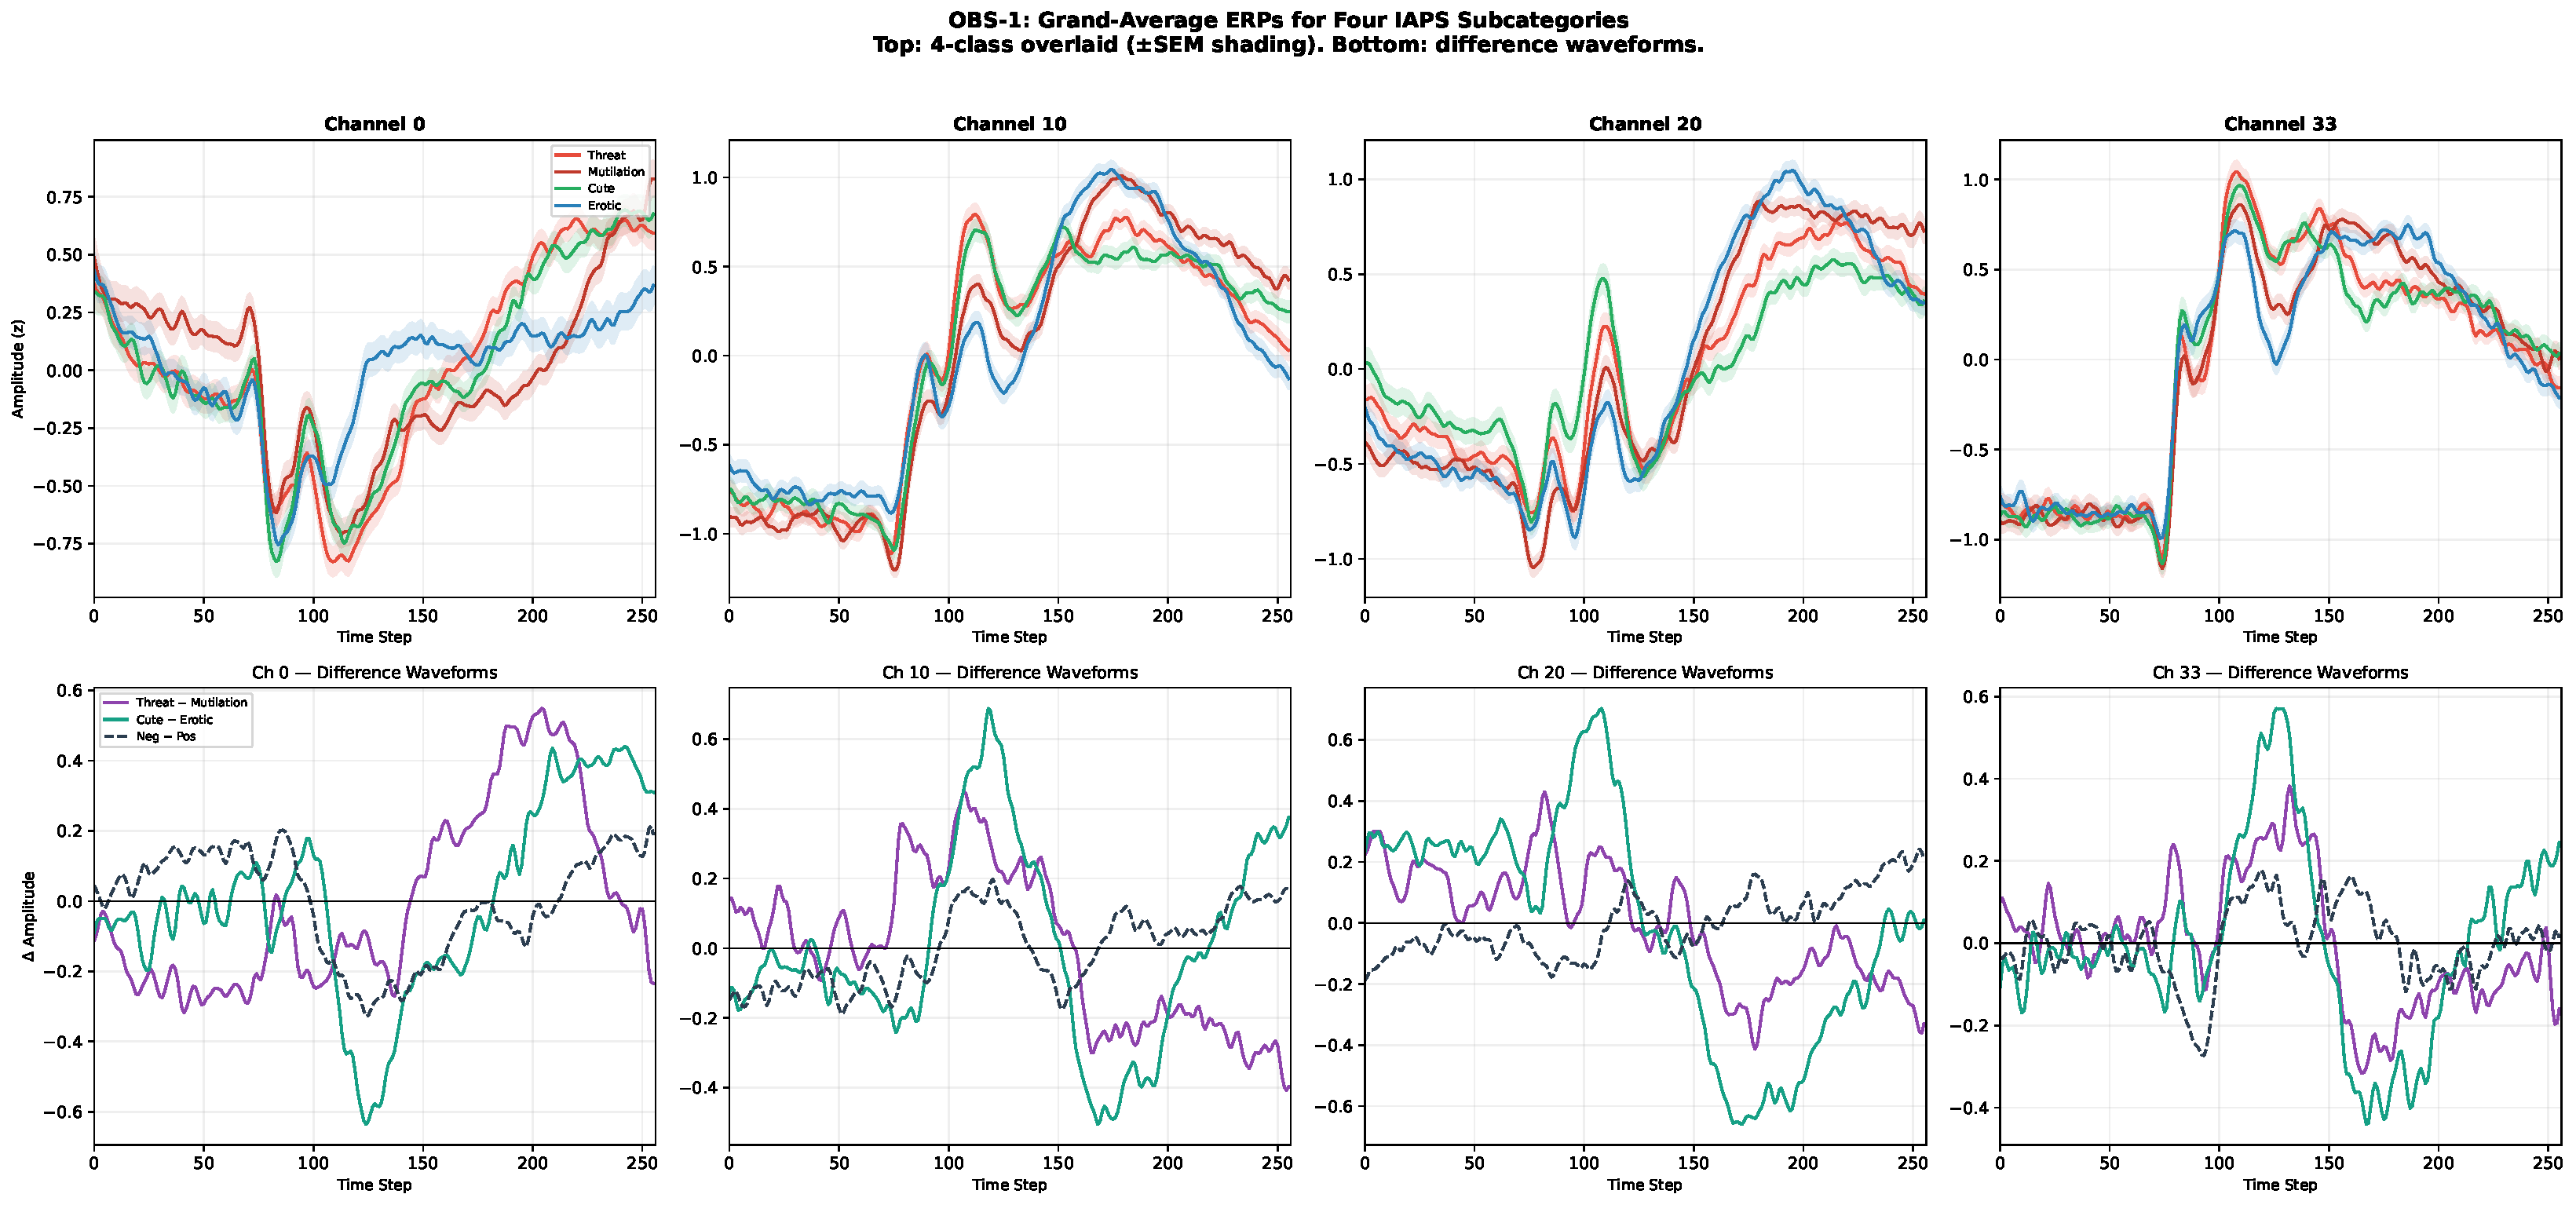
\includegraphics[width=\textwidth]{pictures/appendixA/ch5_4class_obs01_erps.pdf}
    \caption{Grand-average waveforms by category ($N=211$). The displayed late-window differences are descriptive; stimulus-level arousal and valence were not modeled separately.}
    \label{fig:app_4class_obs01}
\end{figure}

\begin{figure}[H]
    \centering
    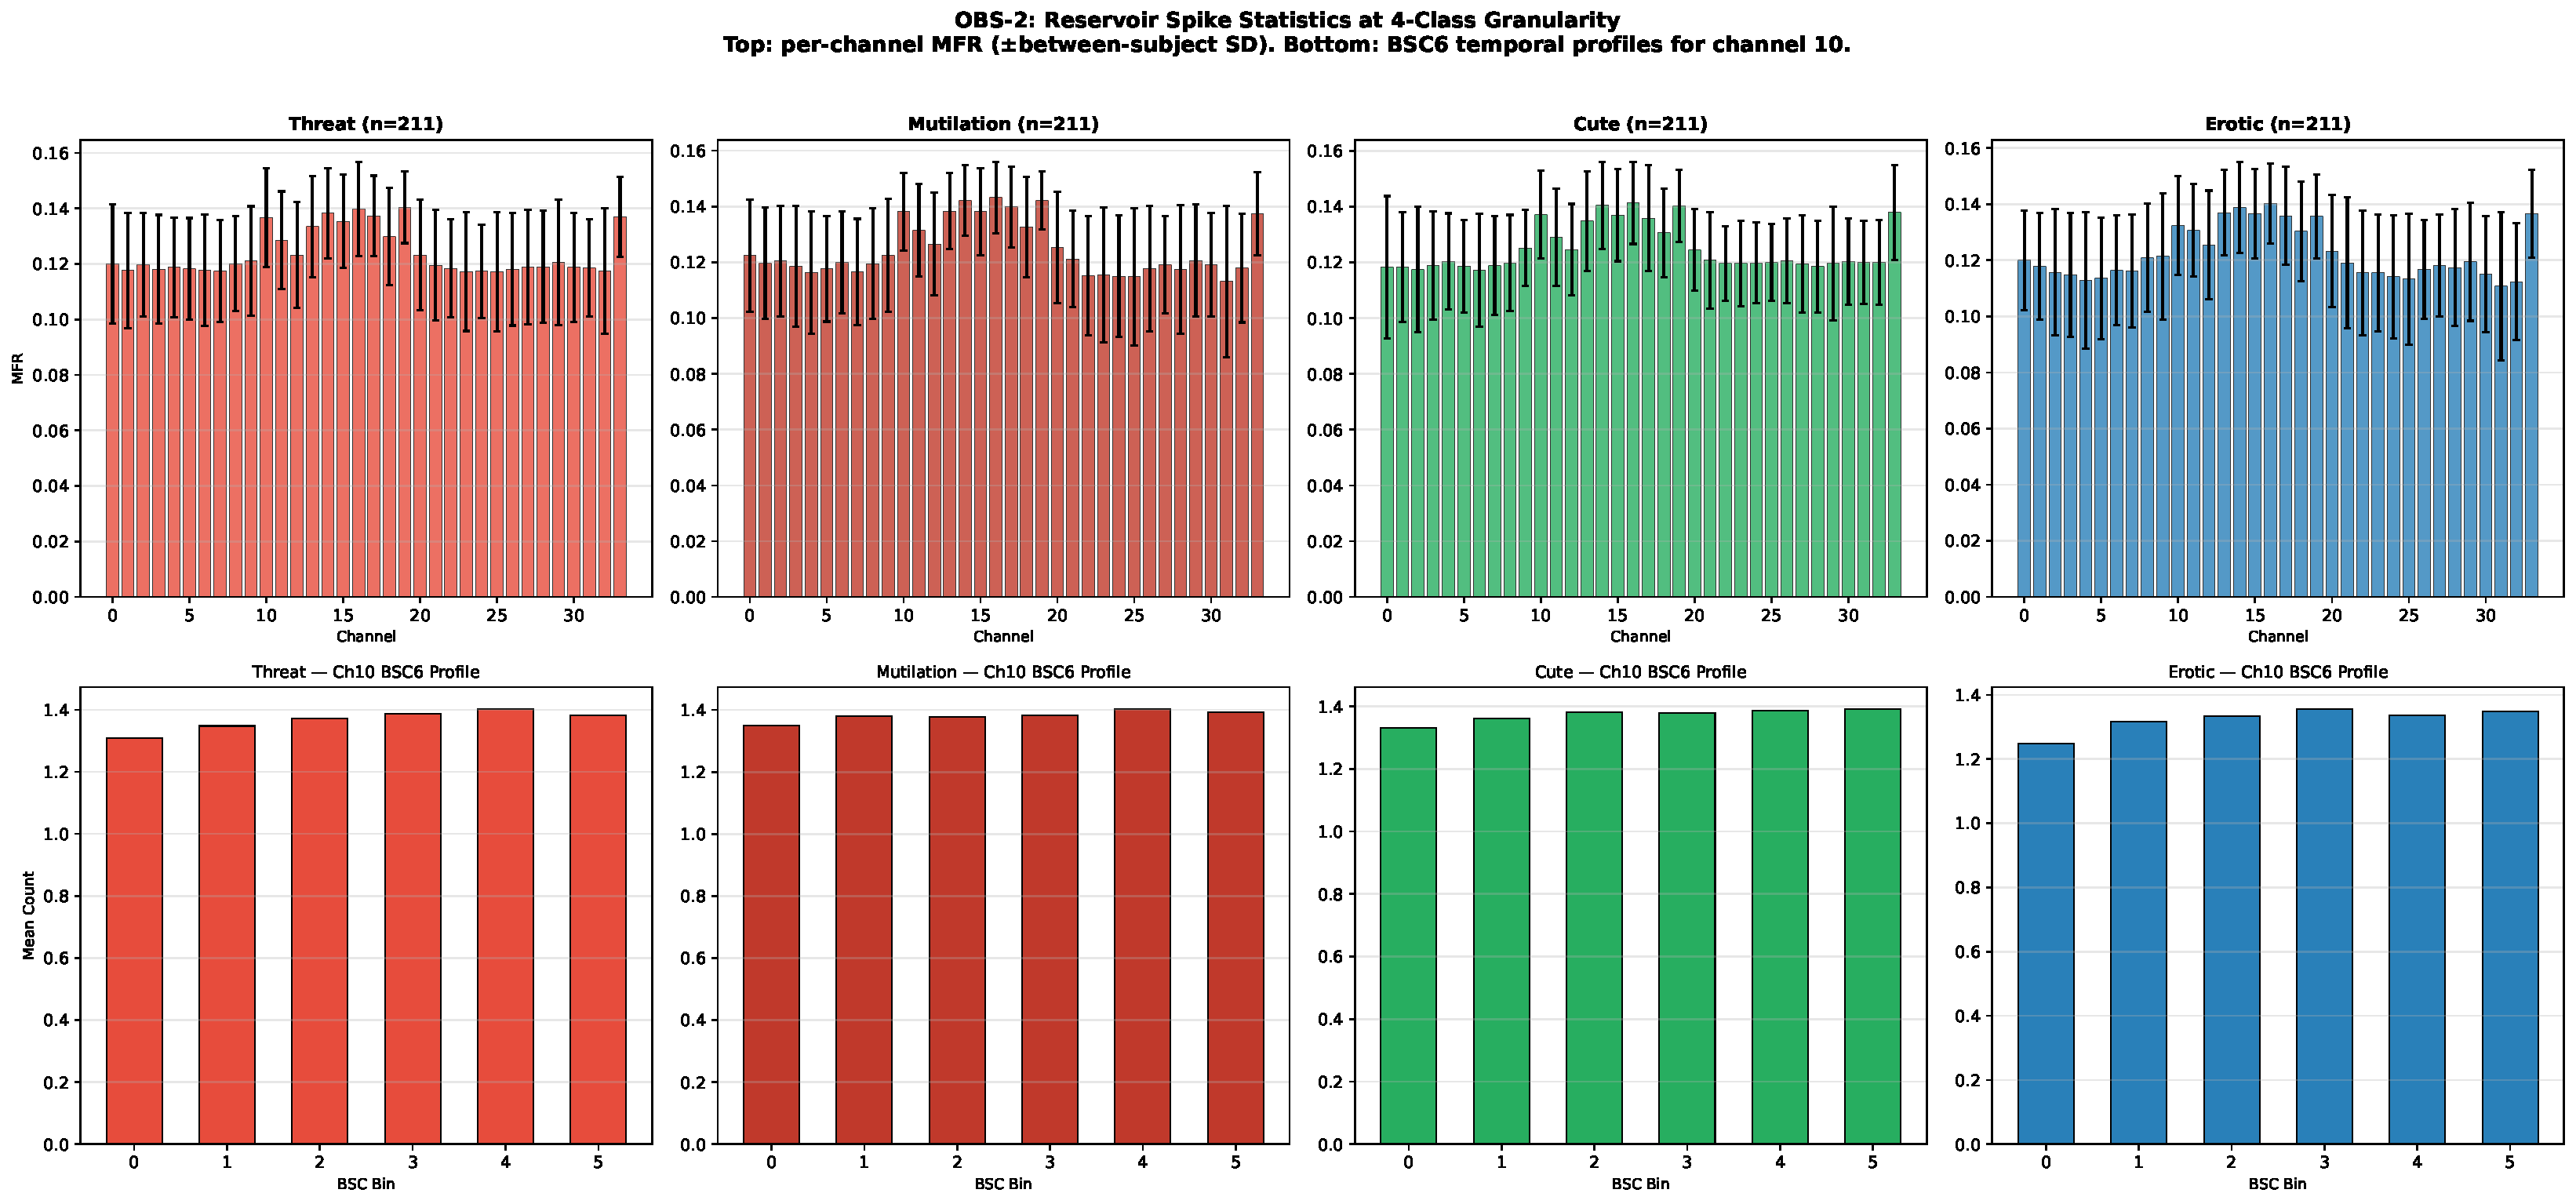
\includegraphics[width=\textwidth]{pictures/appendixA/ch5_4class_obs02_spike_stats.pdf}
    \caption{Archived reservoir spike statistics at four-category resolution: per-channel total spike counts and firing-rate distributions. Gross activation is similar across the displayed category averages; the figure is descriptive and does not test a prespecified channel family.}
    \label{fig:app_4class_obs02}
\end{figure}

\begin{figure}[H]
    \centering
    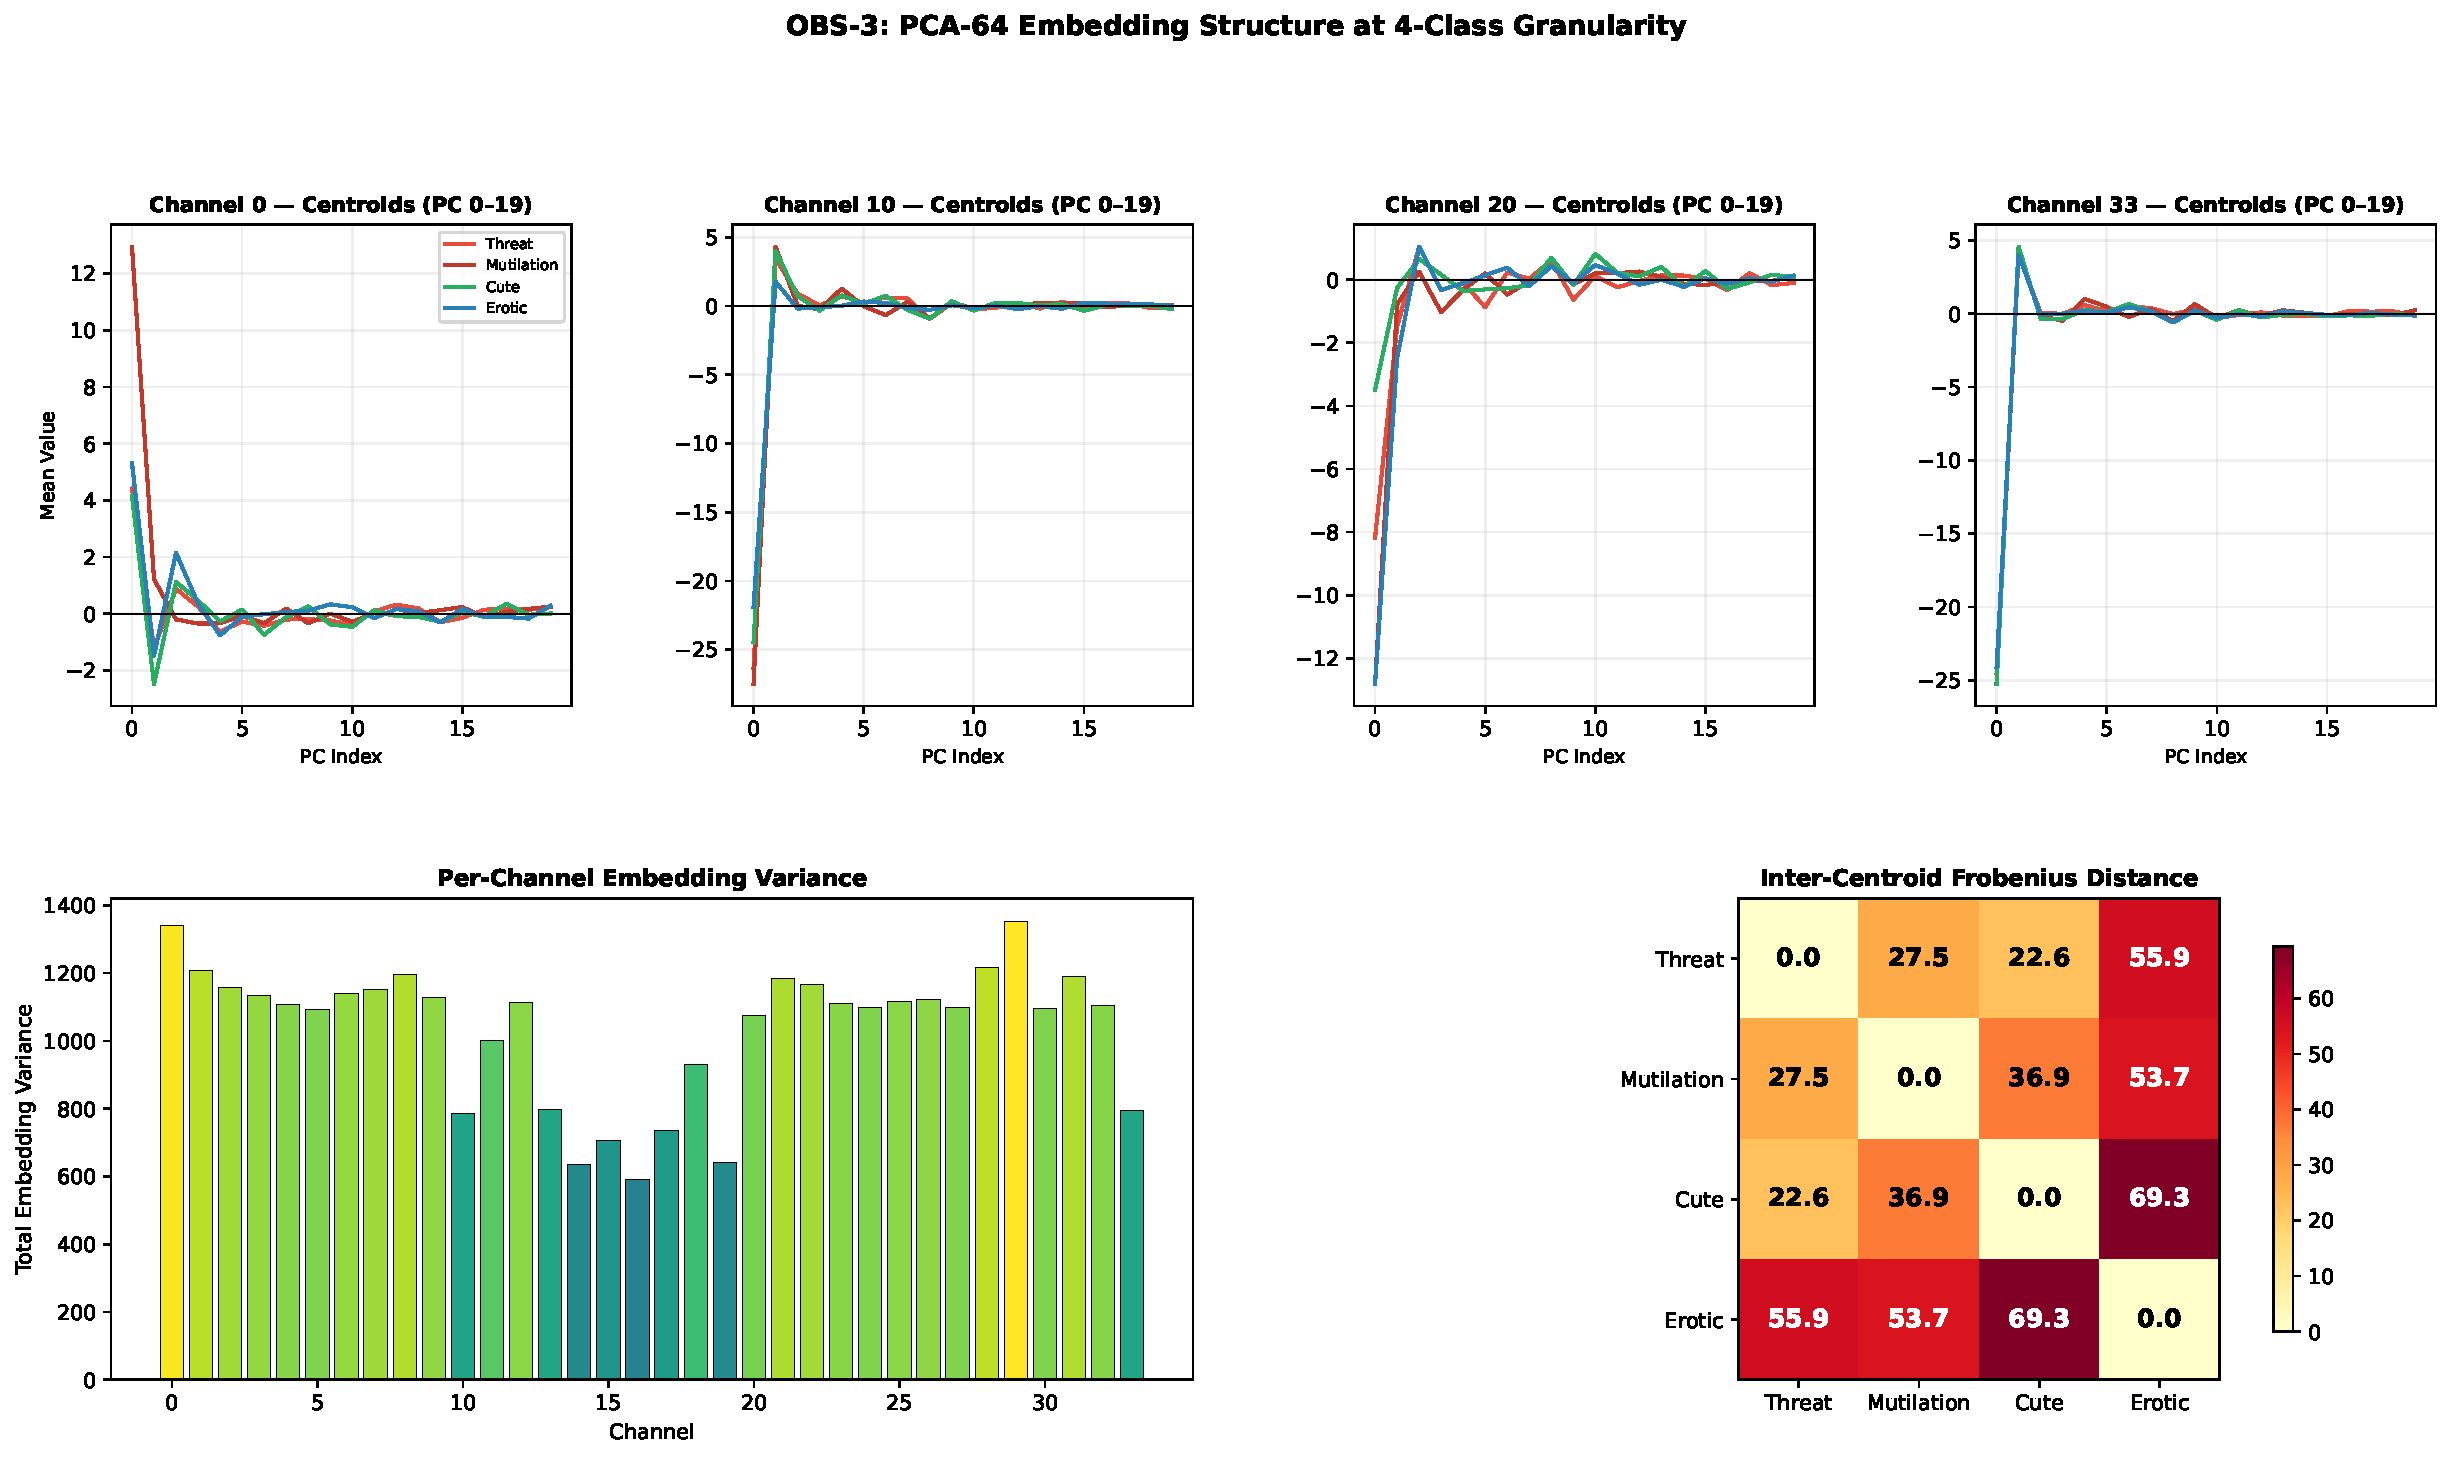
\includegraphics[width=\textwidth]{pictures/appendixA/ch5_4class_obs03_embeddings.pdf}
    \caption{Archived full-sample PCA-64 geometry at four-category resolution. A two-component projection shows substantial category overlap and visible grouping by participant. The reported sums-of-squares fractions are $2.4\%$ for category and $47.0\%$ for participant; because preprocessing and labels differ from the three-condition workflow, the two analyses are not direct replications.}
    \label{fig:app_4class_obs03}
\end{figure}

\begin{figure}[H]
    \centering
    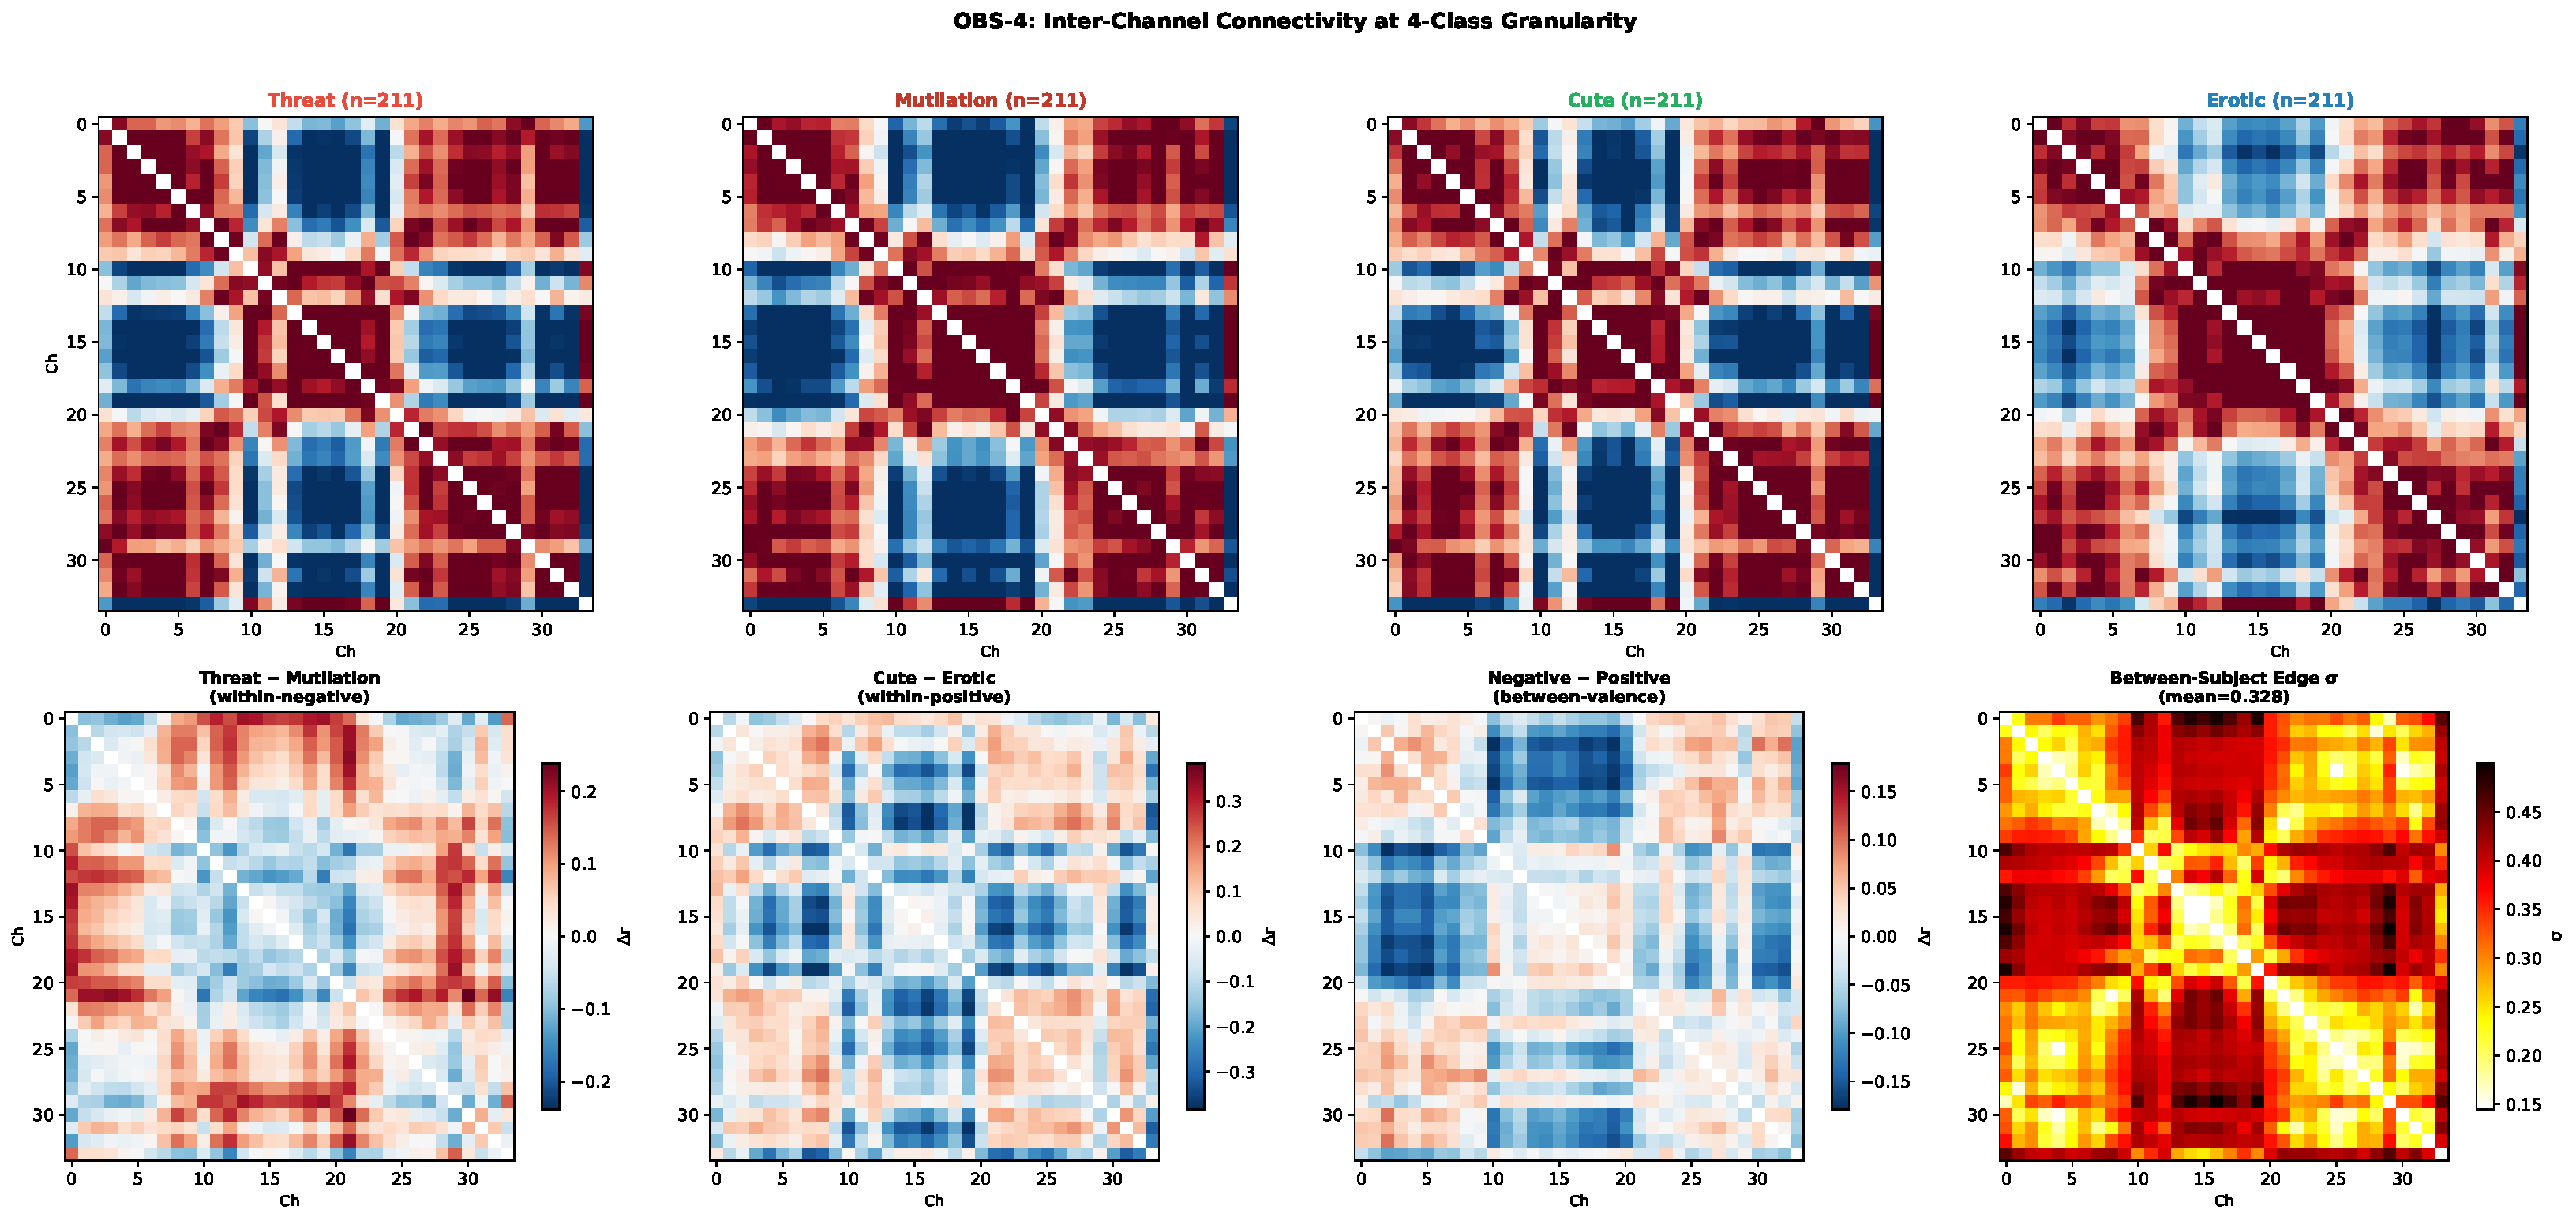
\includegraphics[width=\textwidth]{pictures/appendixA/ch5_4class_obs04_connectivity.pdf}
    \caption{Archived inter-channel representation-similarity matrices and thresholded graph summaries at four-category resolution. The matrices use unlabeled channel indices and full-sample PCA coordinates; they are not estimates of physiological connectivity or anatomical networks.}
    \label{fig:app_4class_obs04}
\end{figure}

\begin{figure}[H]
    \centering
    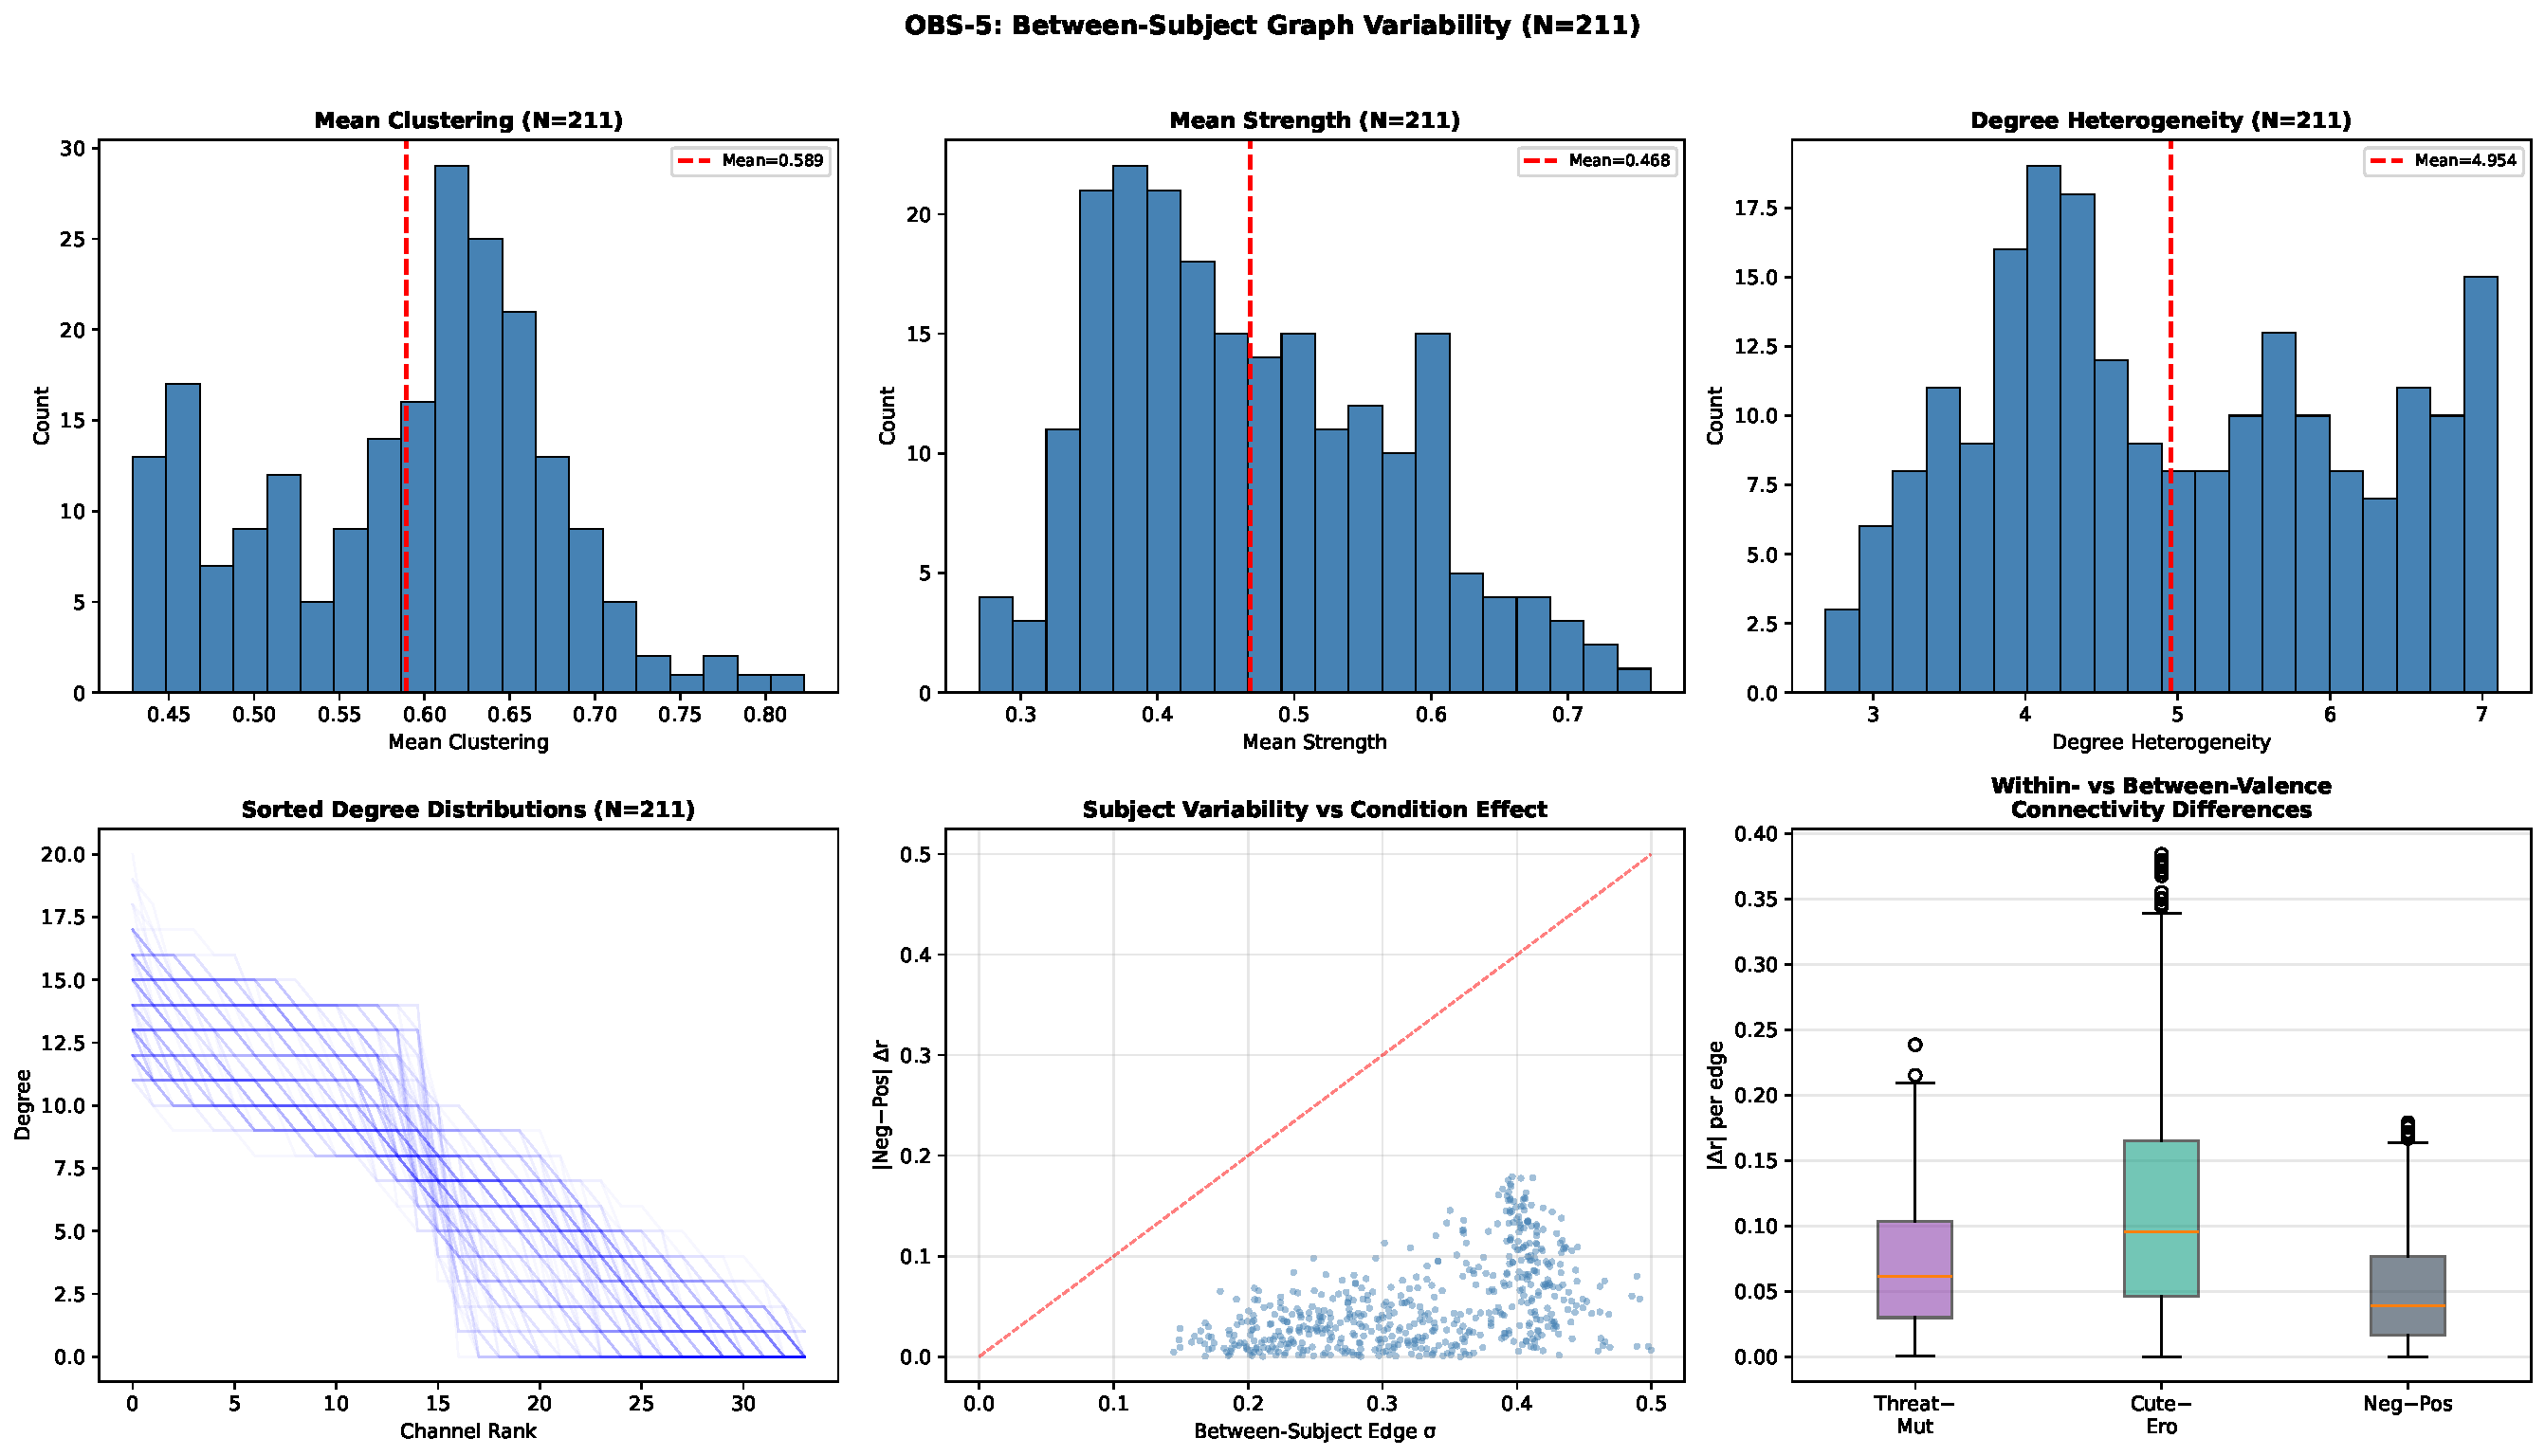
\includegraphics[width=\textwidth]{pictures/appendixA/ch5_4class_obs05_graph_variability.pdf}
    \caption{Archived between-participant graph variability at four-category resolution. The reported participant-to-category sums-of-squares ratio is $19.6\times$, compared with $7.2\times$ in the unmatched three-condition workflow. The ratio is descriptive and does not establish trait stability.}
    \label{fig:app_4class_obs05}
\end{figure}

\begin{figure}[H]
    \centering
    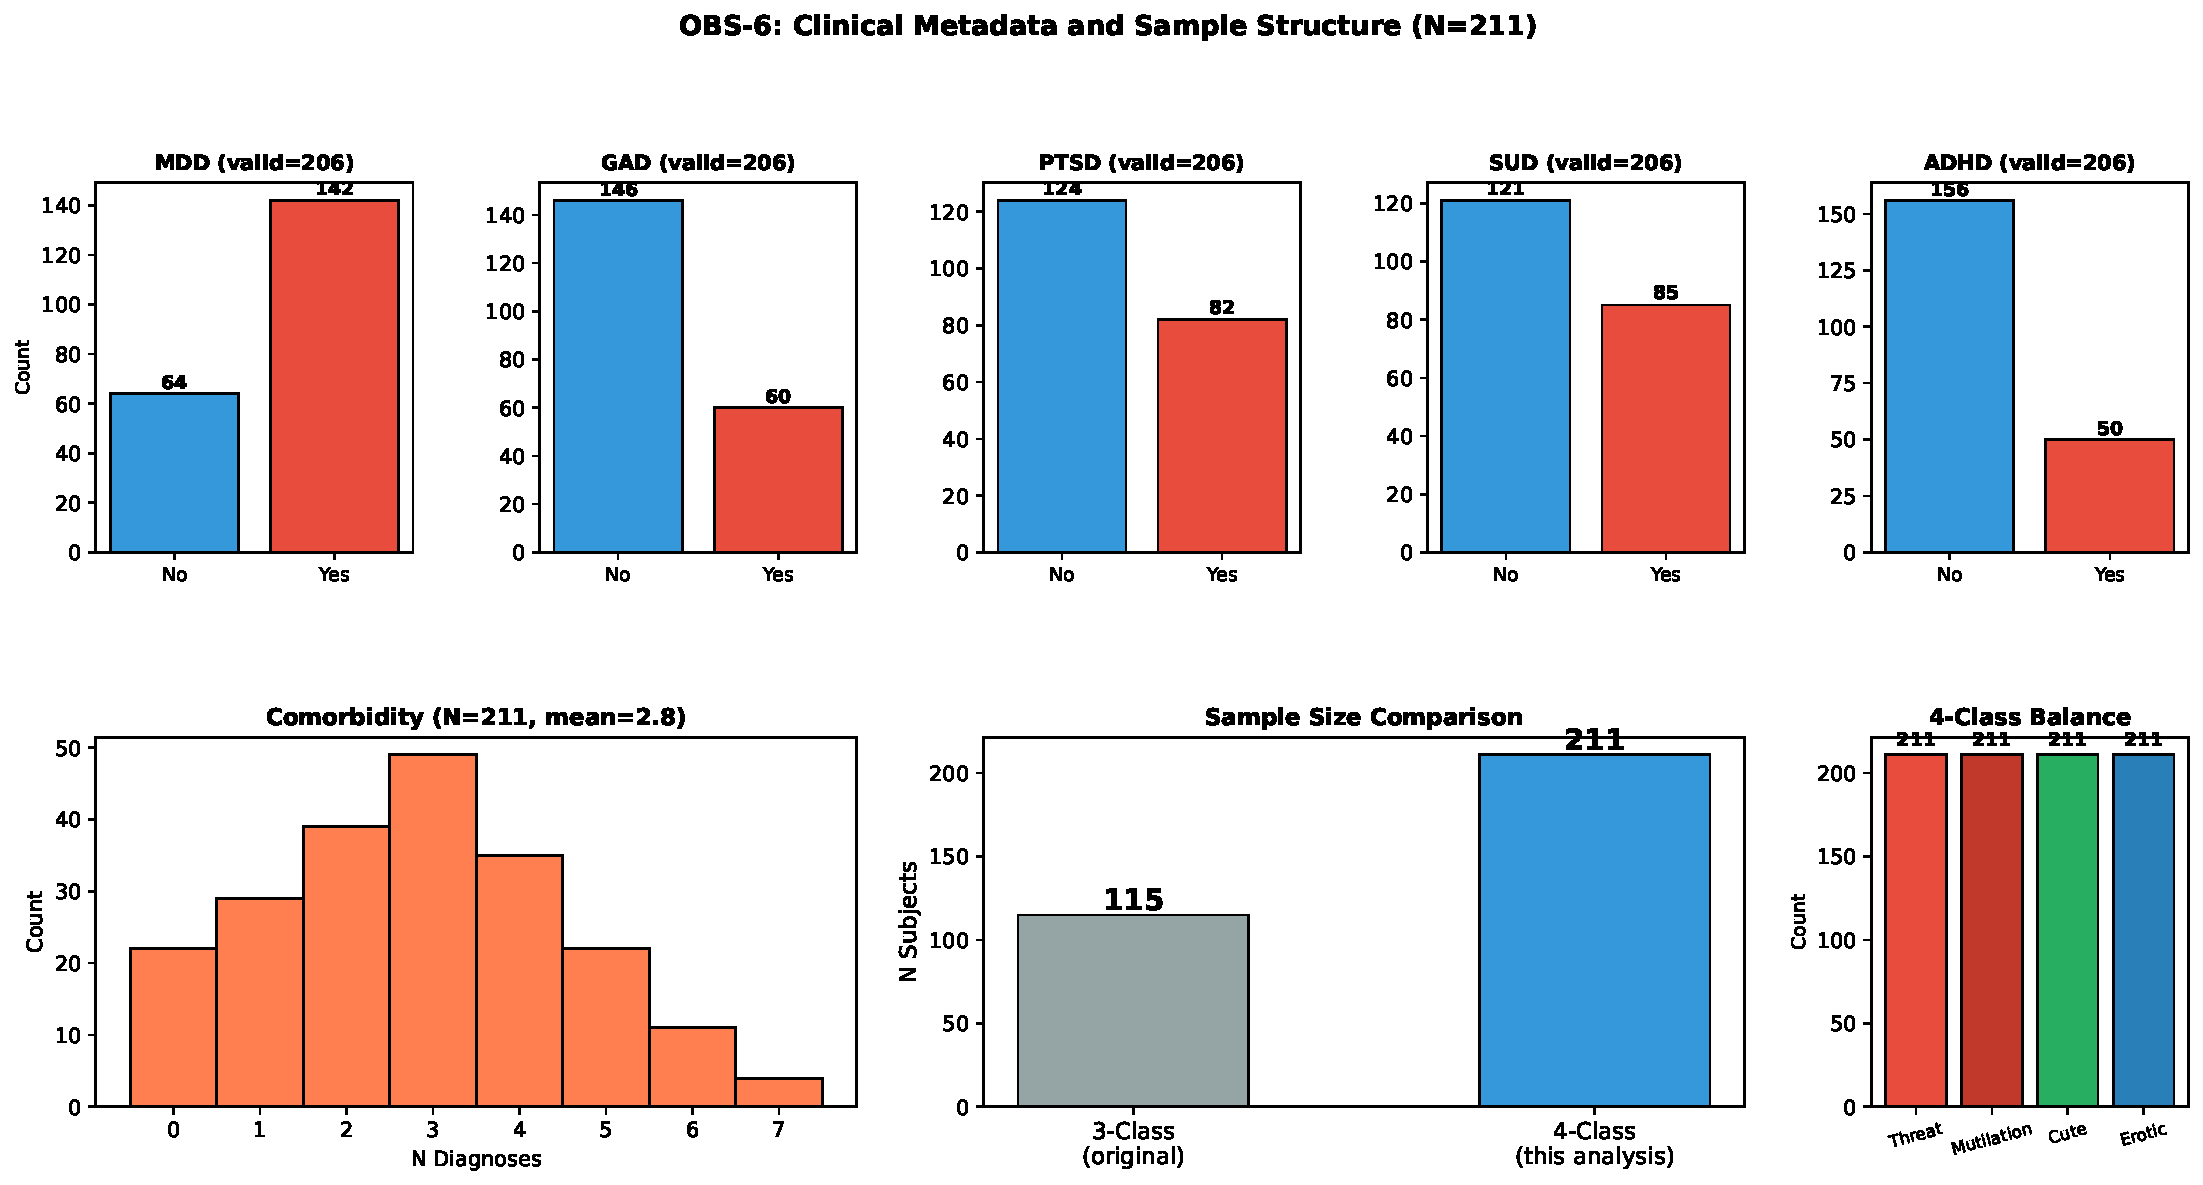
\includegraphics[width=\textwidth]{pictures/appendixA/ch5_4class_obs06_clinical.pdf}
    \caption{Clinical metadata coverage for the four-class analysis ($N = 211$ subjects, $844$ observations). Group sizes and diagnostic distributions are identical to the three-class analysis because the same subjects contribute to both granularities.}
    \label{fig:app_4class_obs06}
\end{figure}

\begin{figure}[H]
    \centering
    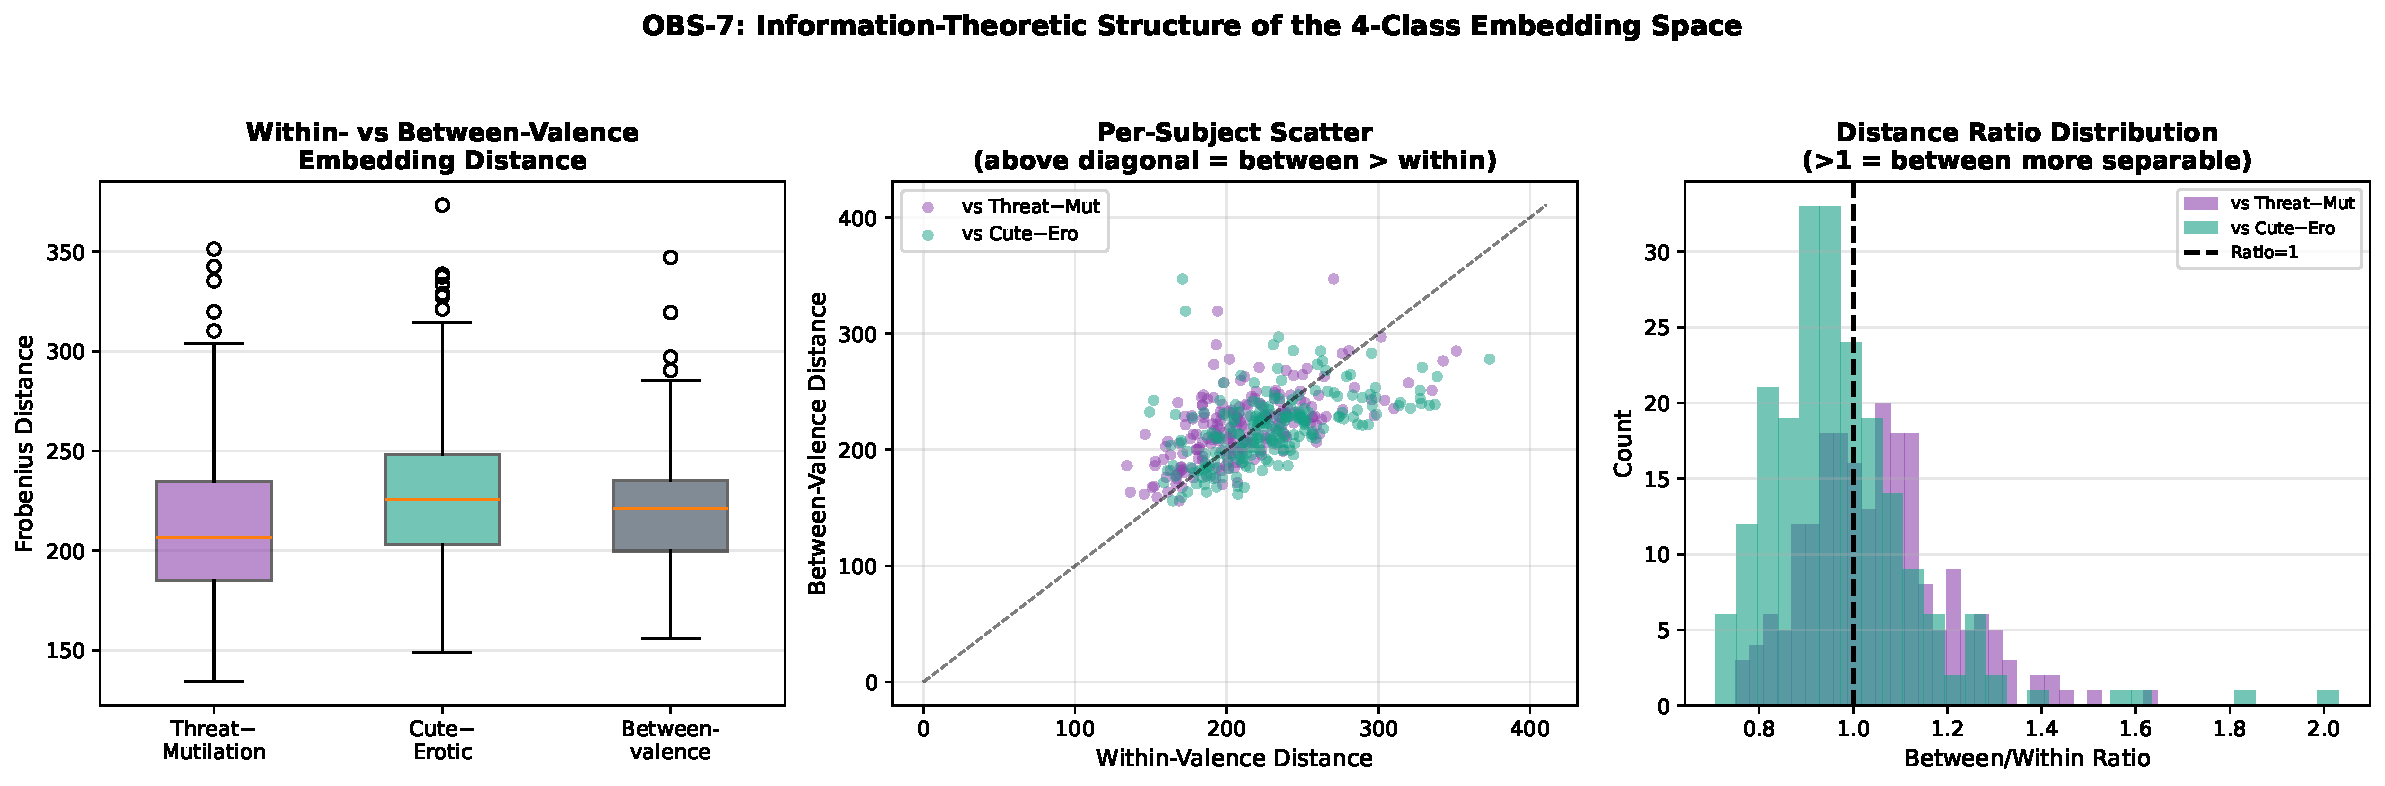
\includegraphics[width=\textwidth]{pictures/appendixA/ch5_4class_obs07_distance_structure.pdf}
    \caption{Archived pairwise distances in the four-category embedding. Threat--Mutilation and Cute--Erotic are grouped as ``within-valence'' in the display. Stimulus-level ratings and potential confounds were not modeled, so the observed distance ordering does not isolate valence or arousal.}
    \label{fig:app_4class_obs07}
\end{figure}


%% ═══════════════════════════════════════════════════════════════
%% SECTION A.2: FOUR-CLASS EXPERIMENTAL RESULTS
%% ═══════════════════════════════════════════════════════════════
\section{Four-Class Classification and Clinical Results}
\label{app:4class}

The following nine figures preserve the archived four-category results discussed in Chapter~\ref{chap:arspi_net}, Section~\ref{sec:ch5_4class}. Their PCA-dependent classification values are descriptive legacy estimates.

\begin{figure}[H]
    \centering
    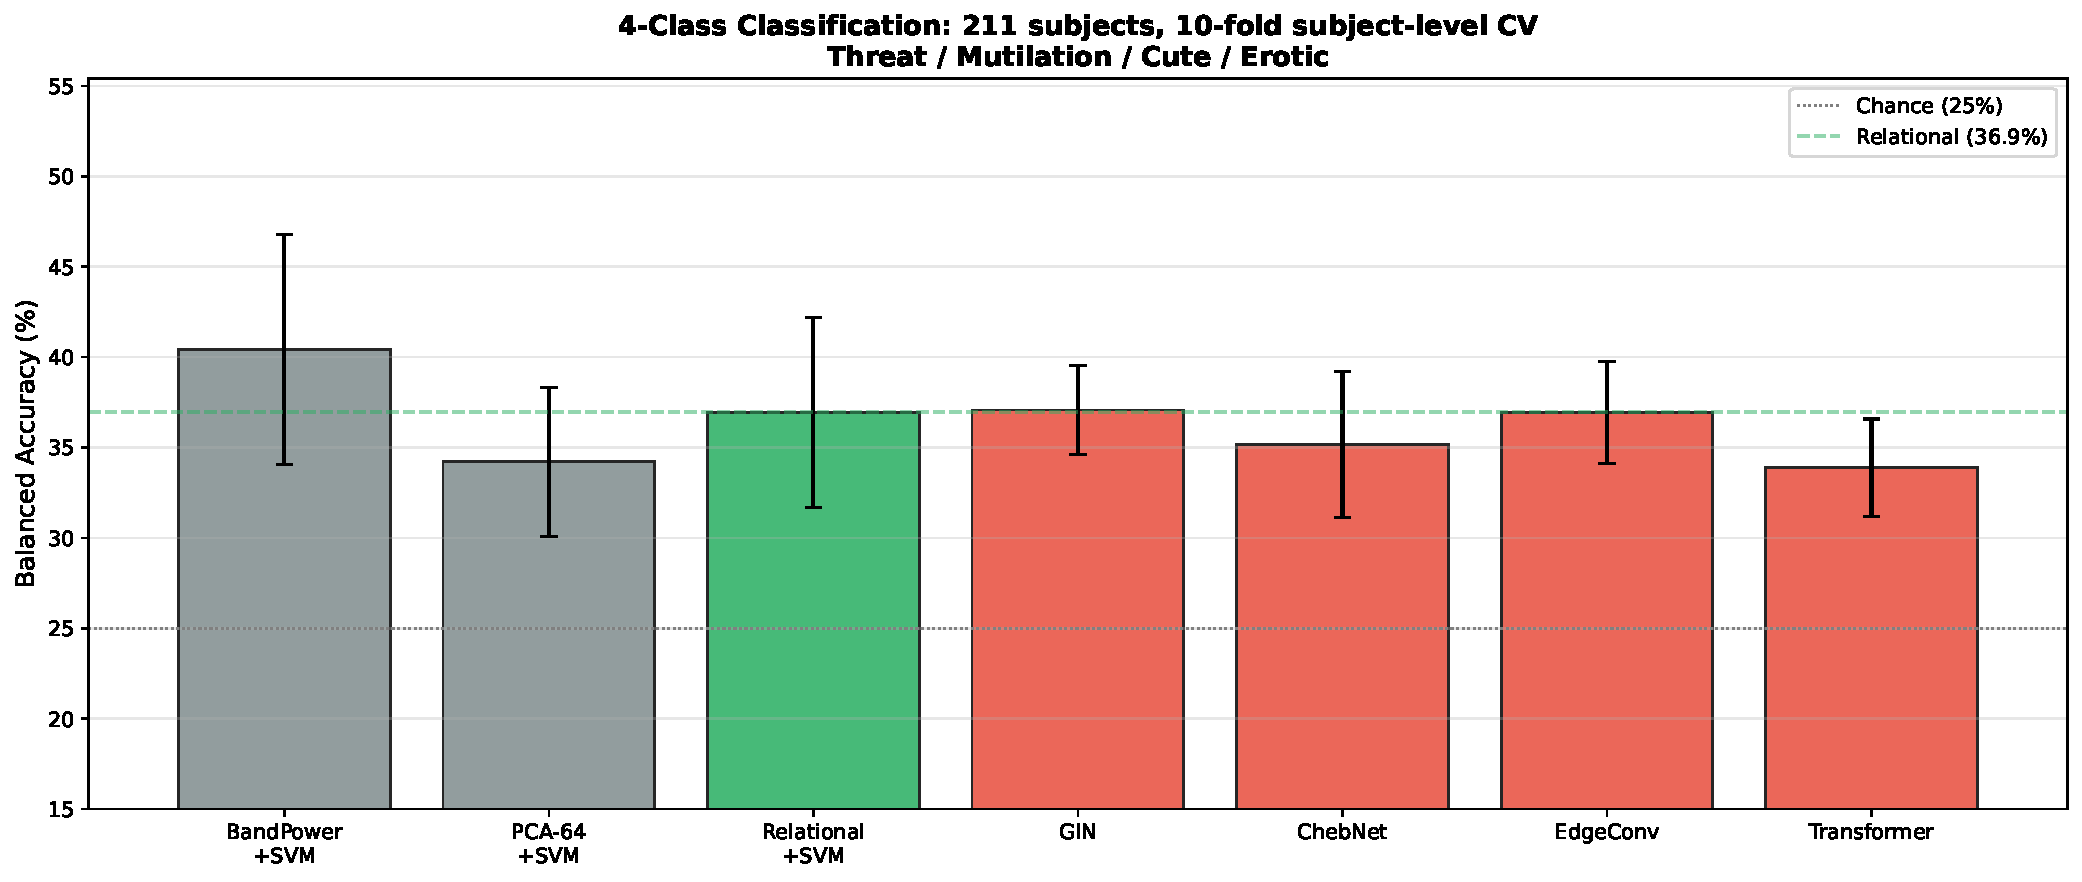
\includegraphics[width=\textwidth]{pictures/appendixA/ch5_4class_fig01_gnn_comparison.pdf}
    \caption{Archived four-category classification comparison ($N=211$, 844 observations). Band-power is 40.4\% and the reservoir embedding 34.2\%. The unmatched three- and four-condition pipelines do not support a replication or regime-boundary claim.}
    \label{fig:app_4class_fig01}
\end{figure}

\begin{figure}[H]
    \centering
    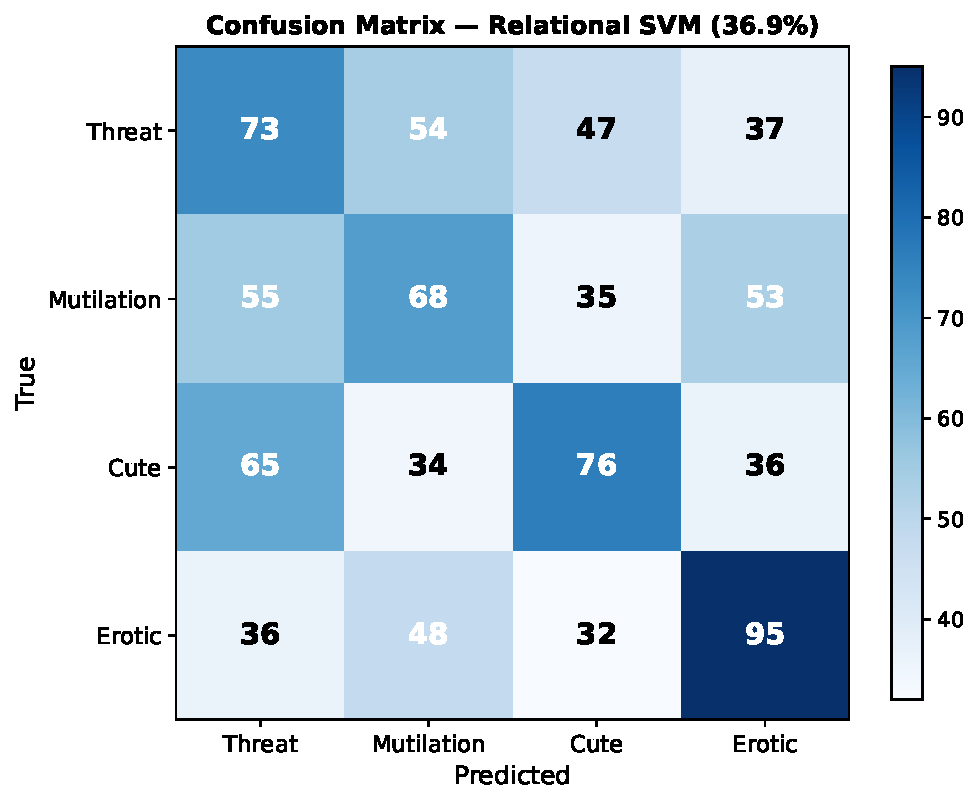
\includegraphics[width=\textwidth]{pictures/appendixA/ch5_4class_fig02_confusion_matrix.pdf}
    \caption{Archived four-category confusion matrix. Threat$\leftrightarrow$Mutilation and Cute$\leftrightarrow$Erotic errors account for $33\%$ of misclassifications. This error count does not by itself establish a valence-organized geometry.}
    \label{fig:app_4class_fig02}
\end{figure}

\begin{figure}[H]
    \centering
    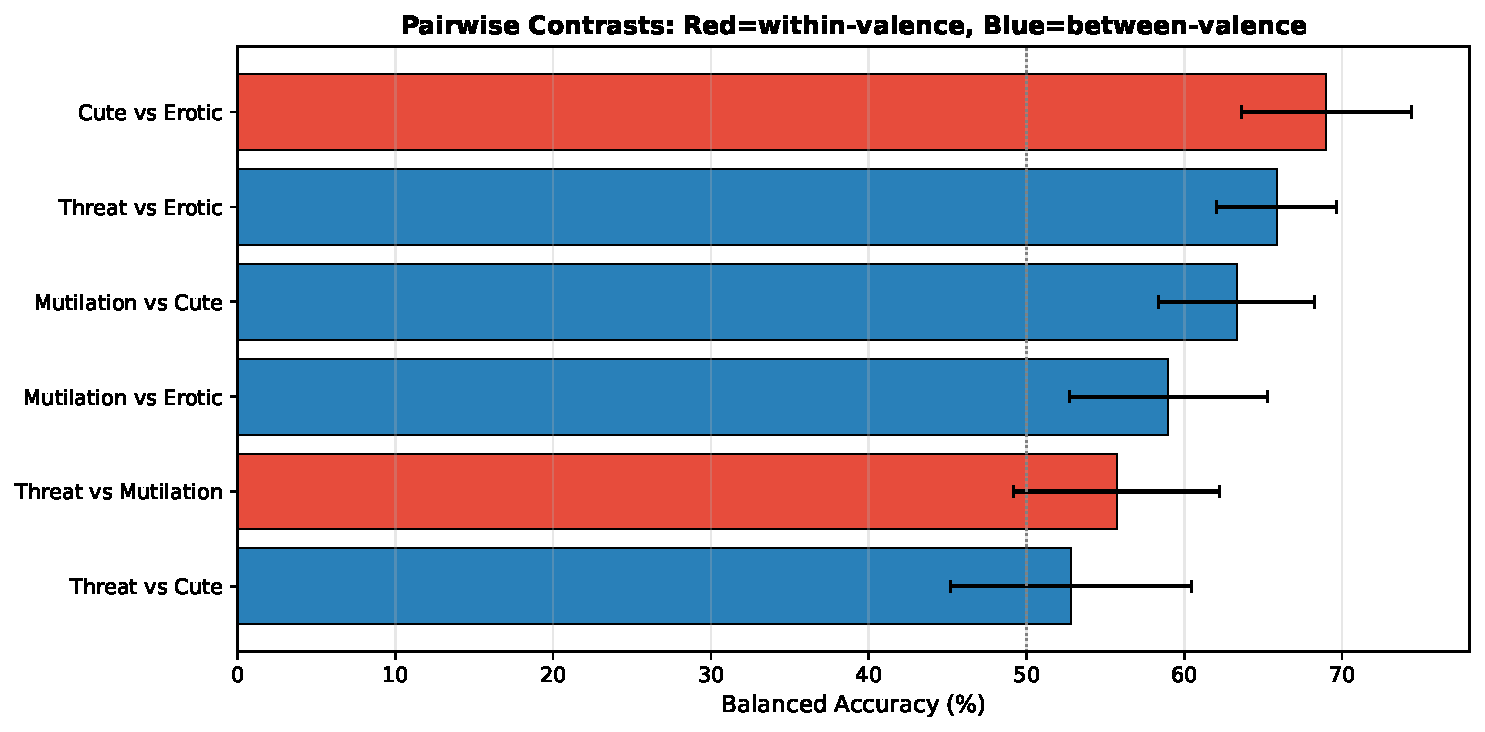
\includegraphics[width=\textwidth]{pictures/appendixA/ch5_4class_fig03_pairwise_contrasts.pdf}
    \caption{Archived pairwise four-category accuracies. Cute versus Erotic is highest (69.0\%) and Threat versus Cute lowest (52.8\%). Because stimulus-level arousal and valence scores were not modeled and the contrasts differ in multiple properties, the ranking does not isolate an arousal effect.}
    \label{fig:app_4class_fig03}
\end{figure}

\begin{figure}[H]
    \centering
    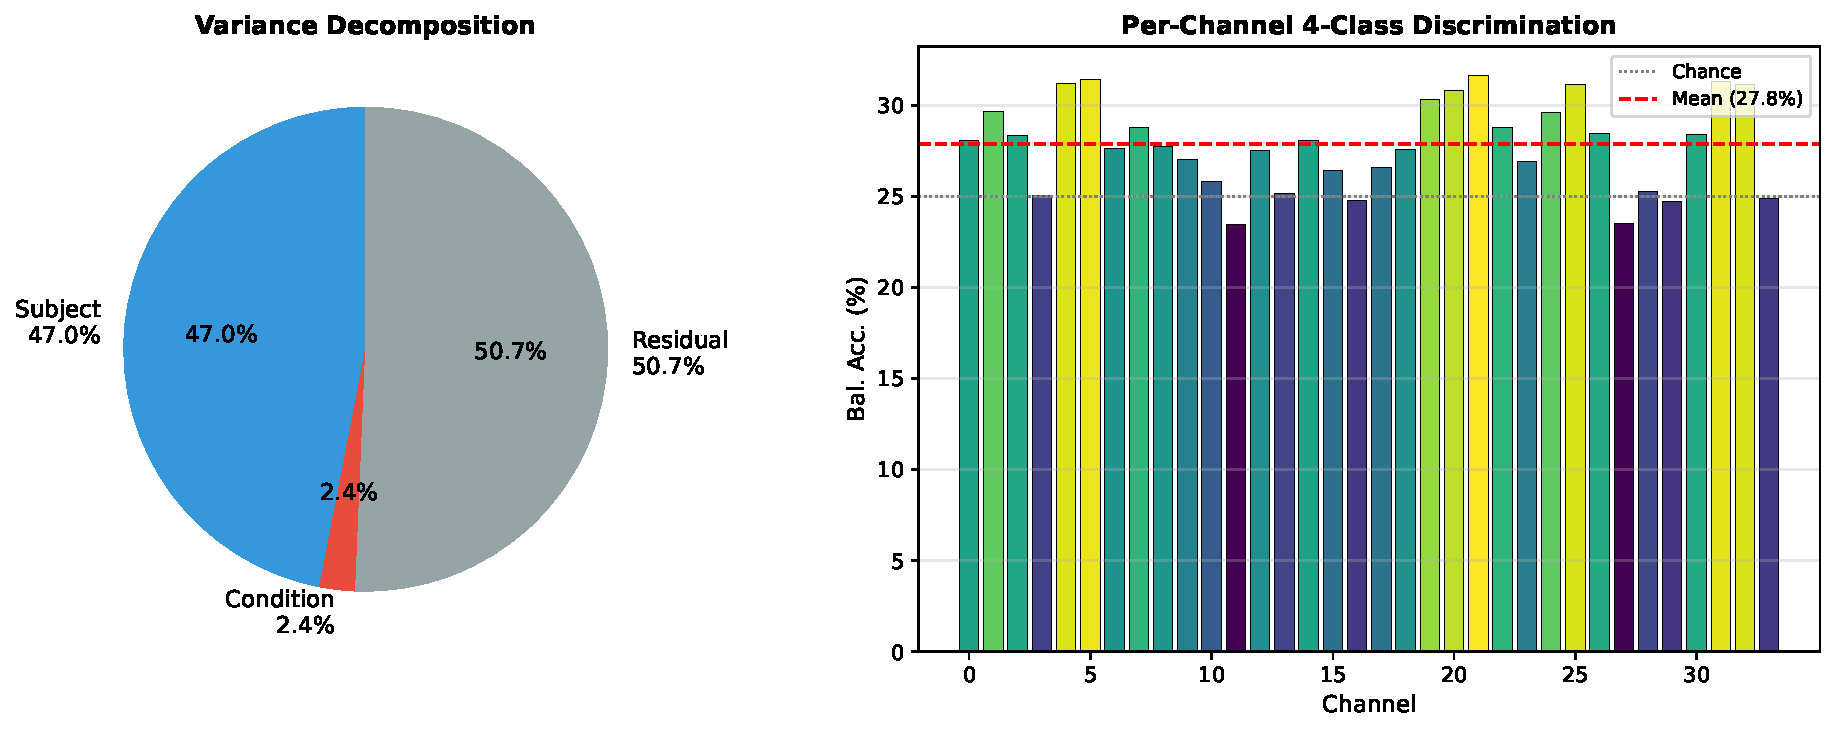
\includegraphics[width=\textwidth]{pictures/appendixA/ch5_4class_fig04_variance_channels.pdf}
    \caption{Archived sums-of-squares decomposition and per-channel analysis at four-category resolution. Participant, category, and residual fractions are $47.0\%$, $2.4\%$, and $50.7\%$, respectively. The unmatched three-condition fractions are shown for context, not as an independent replication.}
    \label{fig:app_4class_fig04}
\end{figure}

\begin{figure}[H]
    \centering
    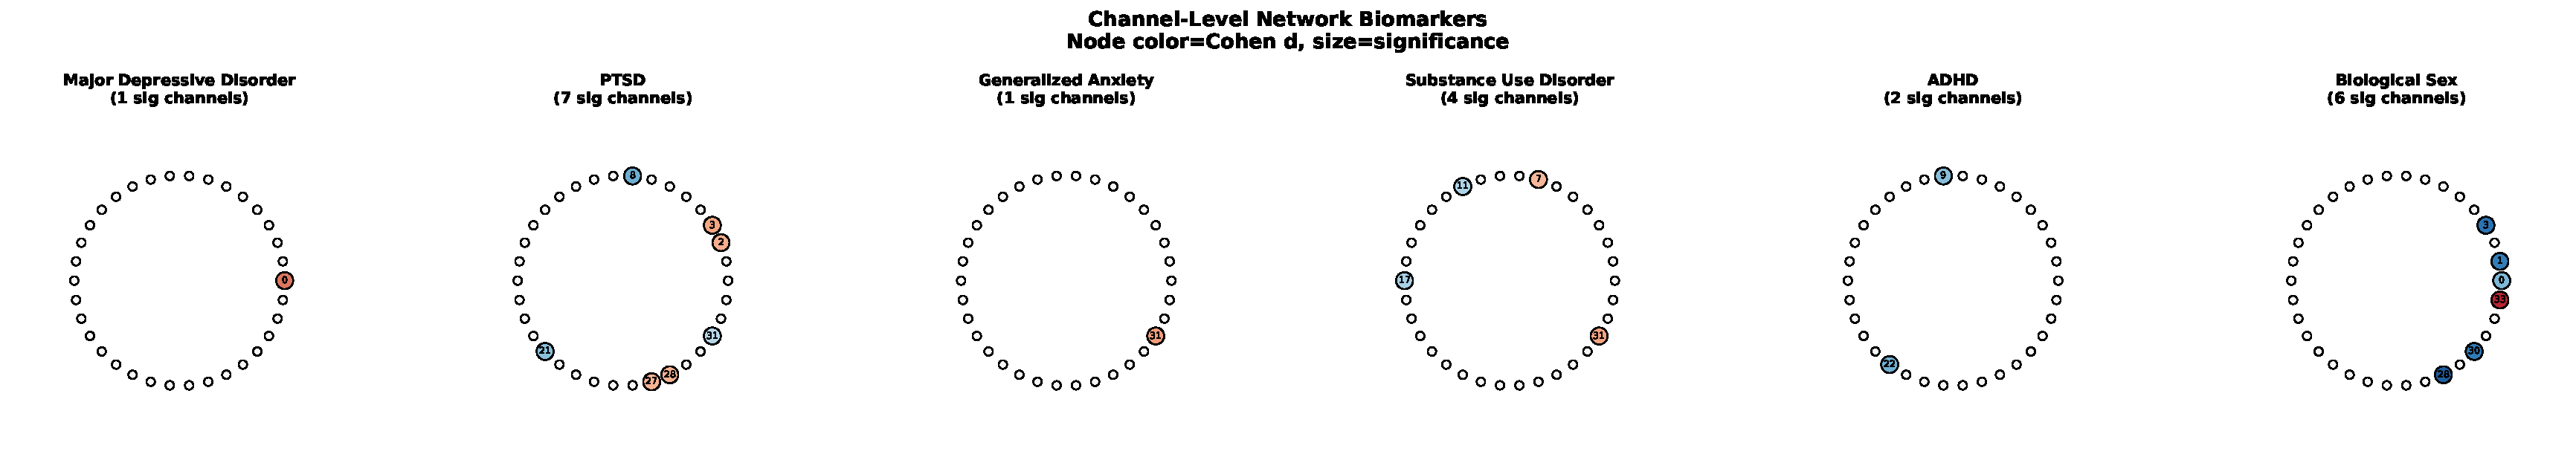
\includegraphics[width=\textwidth]{pictures/appendixA/ch5_4class_fig05_channel_biomarkers.pdf}
    \caption{Uncorrected four-category channel--metric clinical screens. Eleven PTSD cells have nominal $p<0.05$; these are not biomarkers, do not establish disorder-specific spatial signatures, and require correction and external replication.}
    \label{fig:app_4class_fig05}
\end{figure}

\begin{figure}[H]
    \centering
    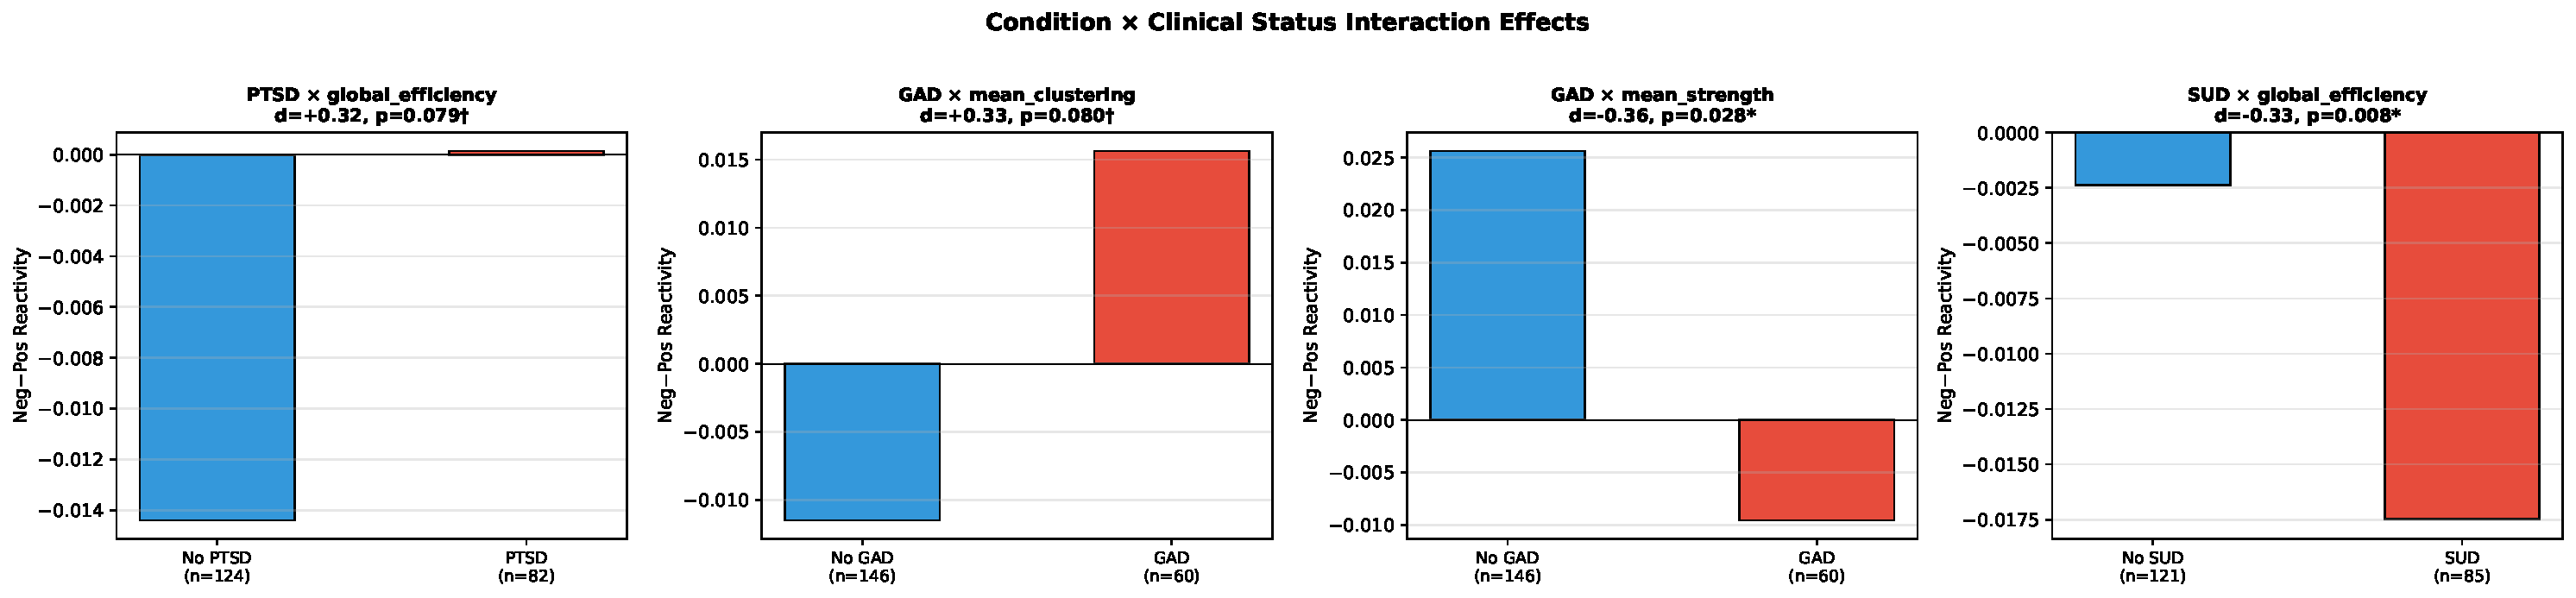
\includegraphics[width=\textwidth]{pictures/appendixA/ch5_4class_fig06_interactions.pdf}
    \caption{Exploratory condition-by-clinical interactions. PTSD by Threat--Mutilation has uncorrected $p=0.036$, and SUD by global efficiency has $p=0.008$ in this pipeline. Neither result is a corrected, independent replication or evidence of network reorganization.}
    \label{fig:app_4class_fig06}
\end{figure}

\begin{figure}[H]
    \centering
    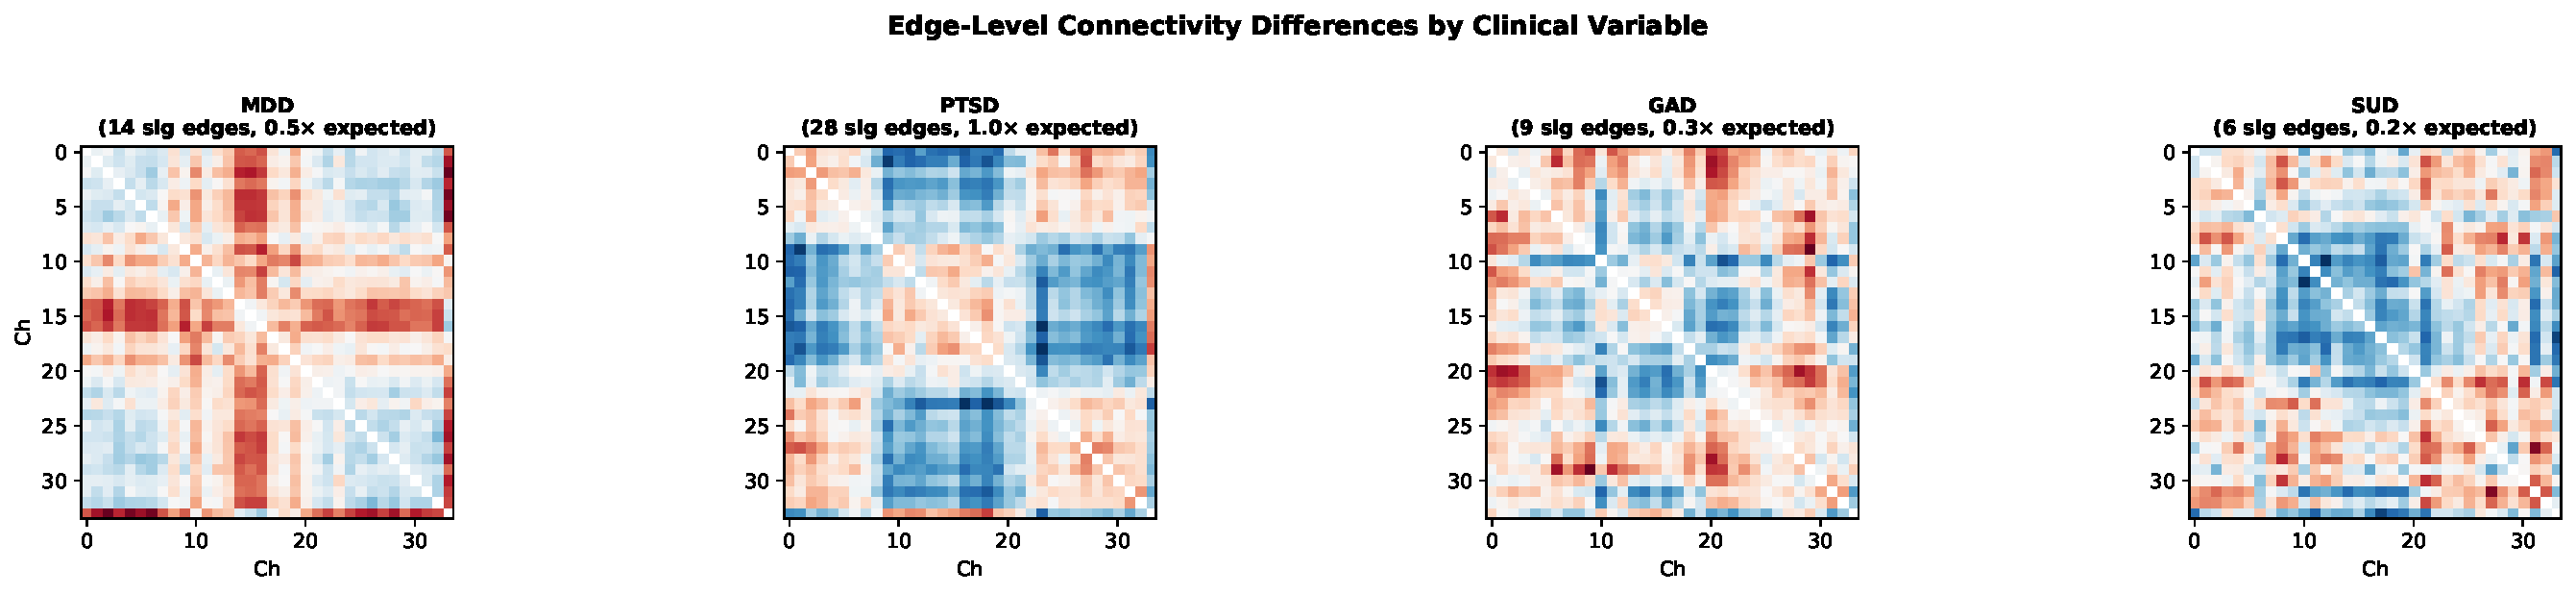
\includegraphics[width=\textwidth]{pictures/appendixA/ch5_4class_fig07_edge_biomarkers.pdf}
    \caption{Four-category edge-level screens. Twenty-eight PTSD edges have nominal significance in the archived analysis; the figure does not establish biomarkers or a granularity effect.}
    \label{fig:app_4class_fig07}
\end{figure}

\begin{figure}[H]
    \centering
    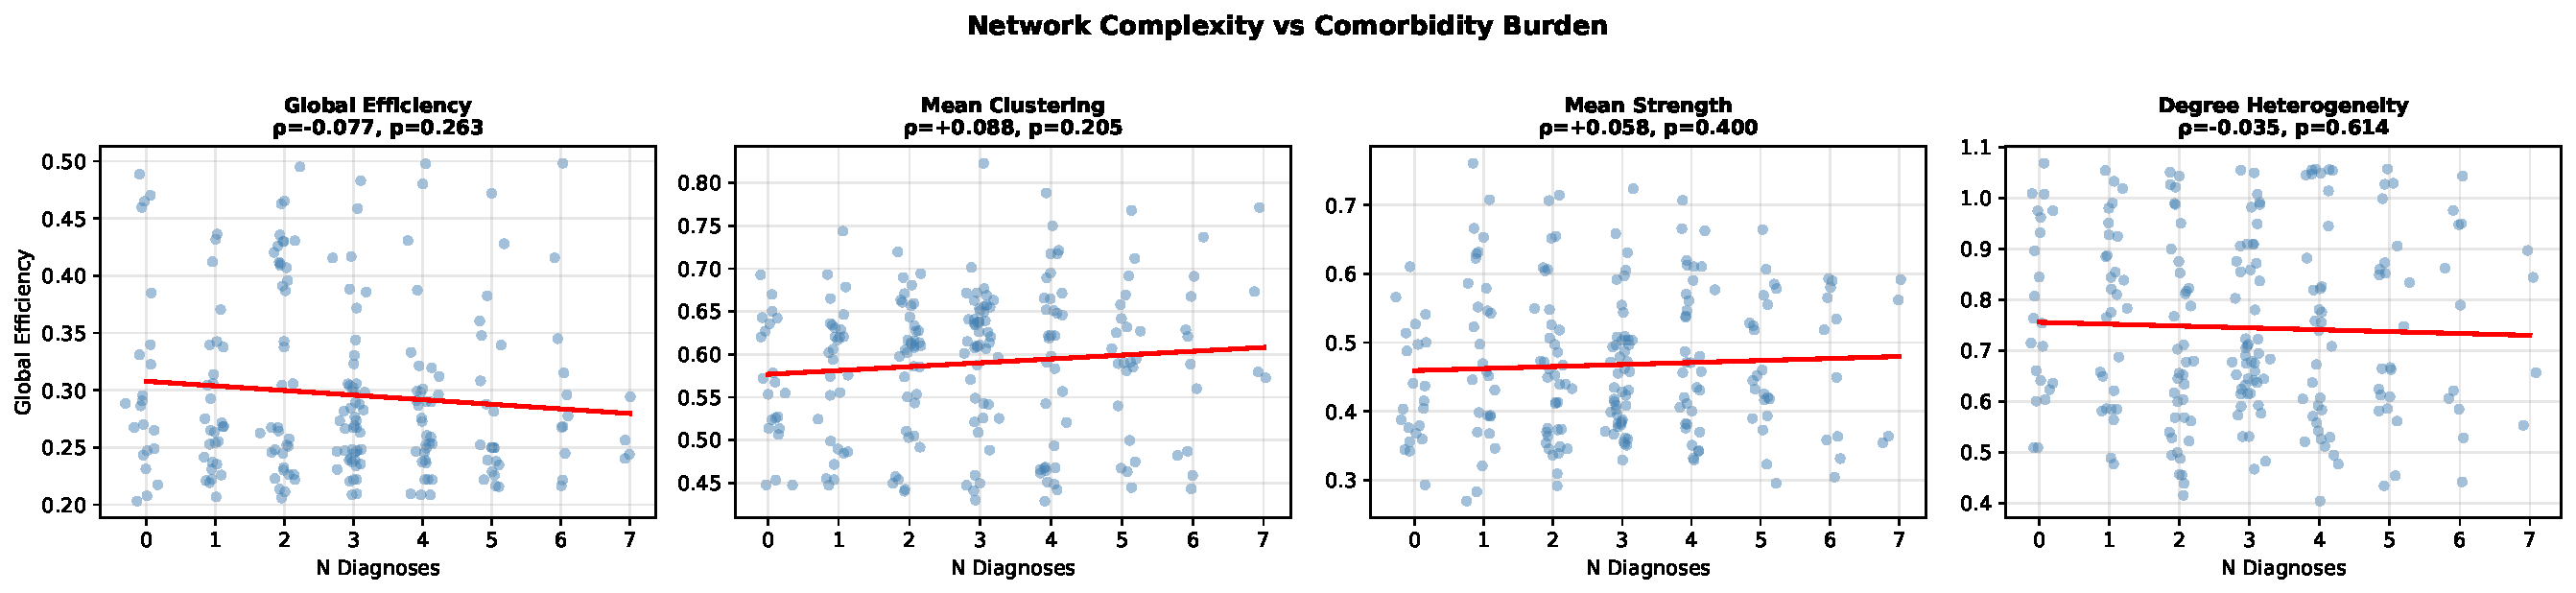
\includegraphics[width=\textwidth]{pictures/appendixA/ch5_4class_fig08_comorbidity.pdf}
    \caption{Comorbidity-count comparisons with graph summaries. Non-significant correlations do not rule out confounding by comorbidity or other clinical variables.}
    \label{fig:app_4class_fig08}
\end{figure}

\begin{figure}[H]
    \centering
    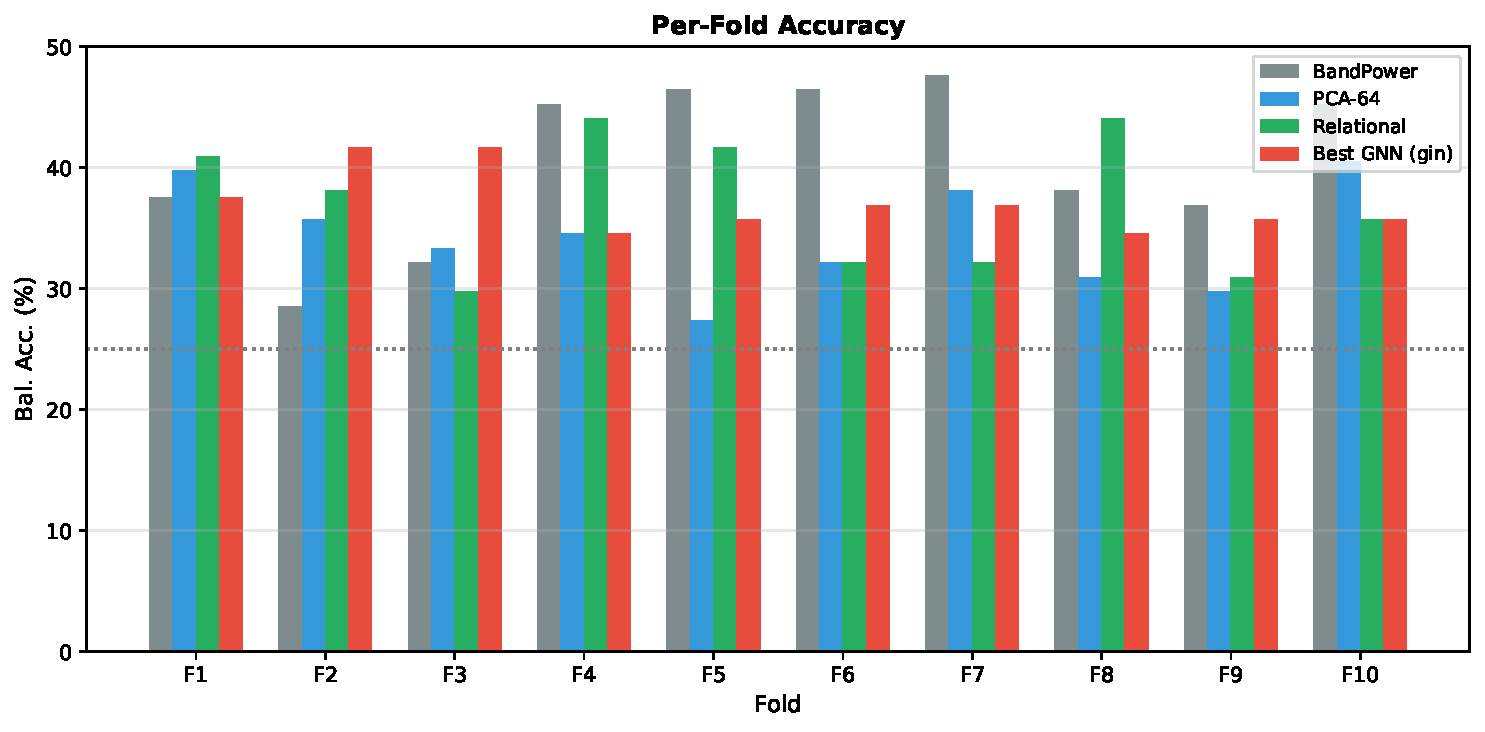
\includegraphics[width=\textwidth]{pictures/appendixA/ch5_4class_fig09_fold_comparison.pdf}
    \caption{Archived per-fold accuracies for band-power, reservoir, and graph classifiers. Folds overlap in training data and do not supply independent evidence of robustness.}
    \label{fig:app_4class_fig09}
\end{figure}


%% ═══════════════════════════════════════════════════════════════
%% SECTION A.3: LAYER ABLATION FIGURES
%% ═══════════════════════════════════════════════════════════════
\section{Layer Ablation and Complementarity Figures}
\label{app:ablation}

The following three figures present the complete visualization of the layer ablation experiment reported in Chapter~\ref{chap:arspi_net}, Section~\ref{sec:ch5_ablation}. The numerical results are presented in Tables~\ref{tab:emotion_ablation} and~\ref{tab:clinical_ablation} in the main text.

\begin{figure}[H]
    \centering
    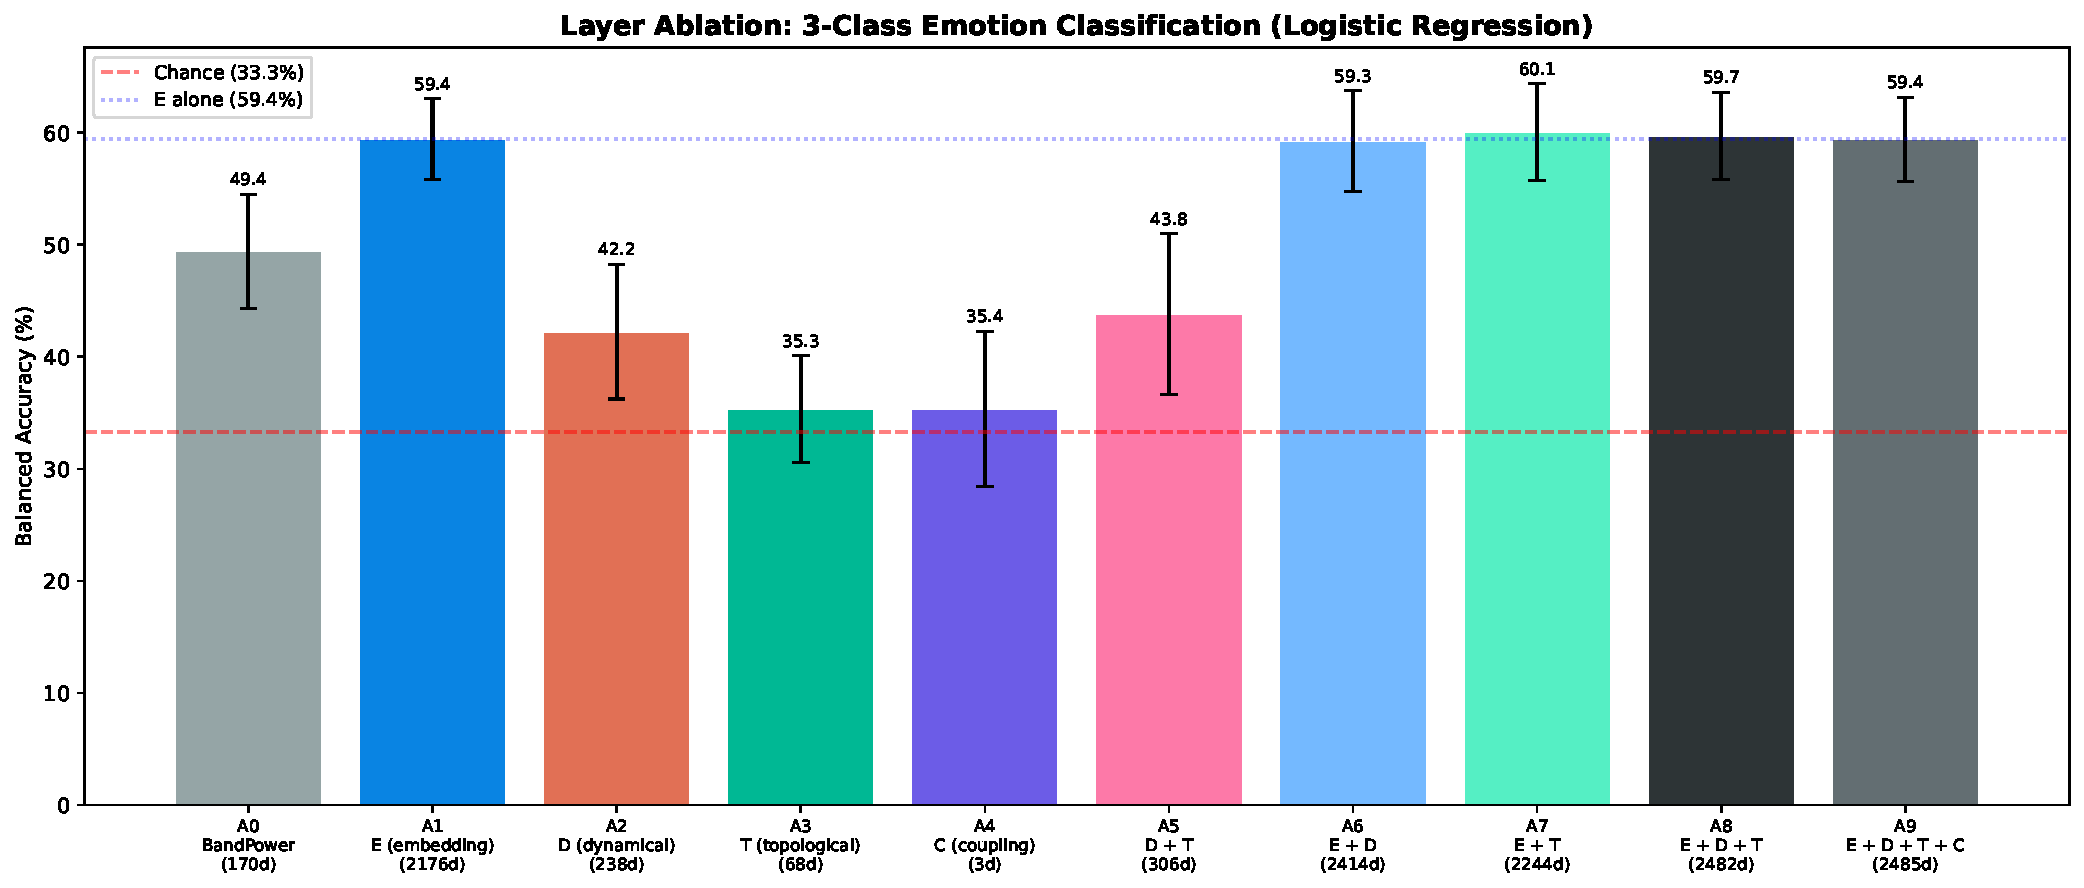
\includegraphics[width=\textwidth]{pictures/appendixA/ch5_fig_emotion_ablation.pdf}
    \caption{Archived three-condition layer comparison (logistic regression, 10 subject-grouped folds). A0: band-power ($49.4\%$); A1: embedding ($59.4\%$); A2: dynamical summaries ($42.2\%$); A3: topological summaries ($35.3\%$); A4: coupling ($35.4\%$); A5--A9: combinations. A1 has the highest recorded mean, and no combination exceeds it by more than $0.7$ percentage points. Fold standard deviations are descriptive because training sets overlap.}
    \label{fig:app_emotion_ablation}
\end{figure}

\begin{figure}[H]
    \centering
    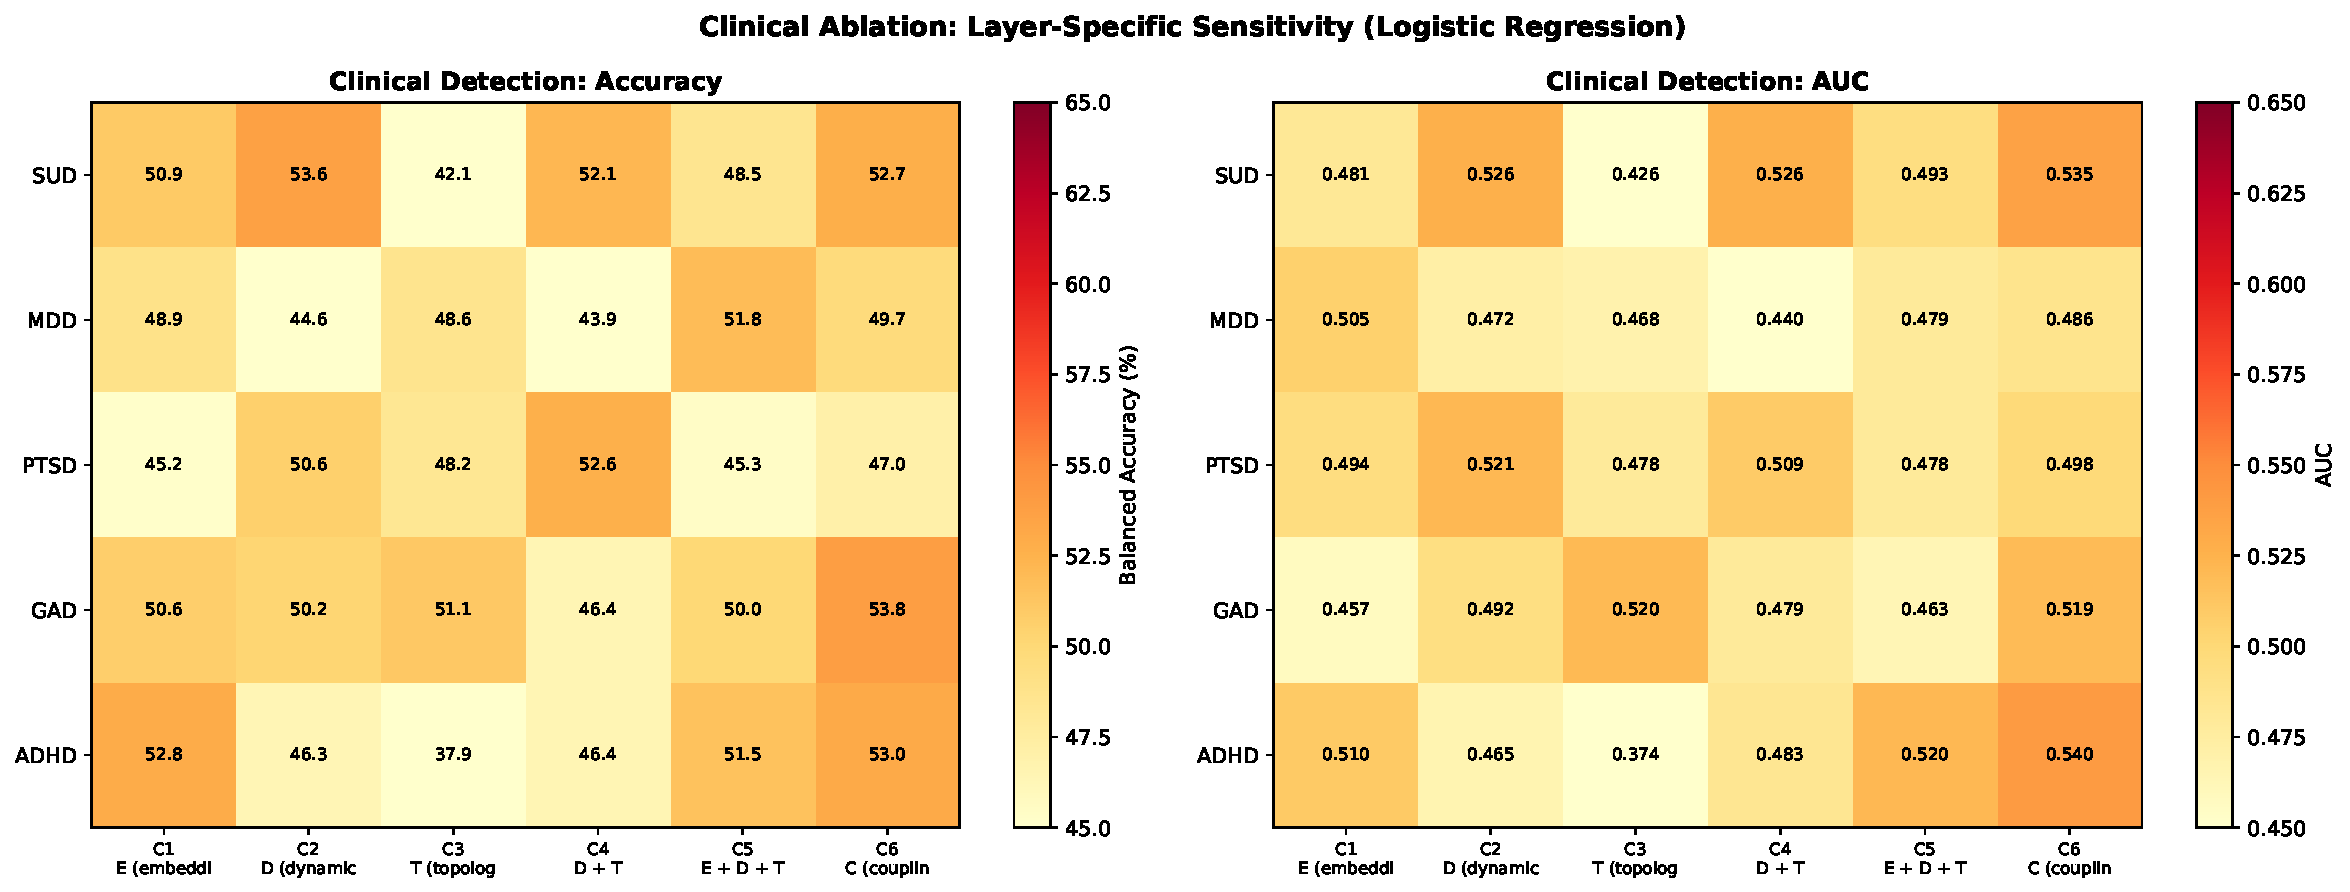
\includegraphics[width=\textwidth]{pictures/appendixA/ch5_fig_clinical_ablation.pdf}
    \caption{Exploratory subject-level five-fold clinical readouts by feature block. The post-hoc maximum differs by label, but near-chance performance and model selection prevent a disorder- or layer-specific claim.}
    \label{fig:app_clinical_ablation}
\end{figure}

\begin{figure}[H]
    \centering
    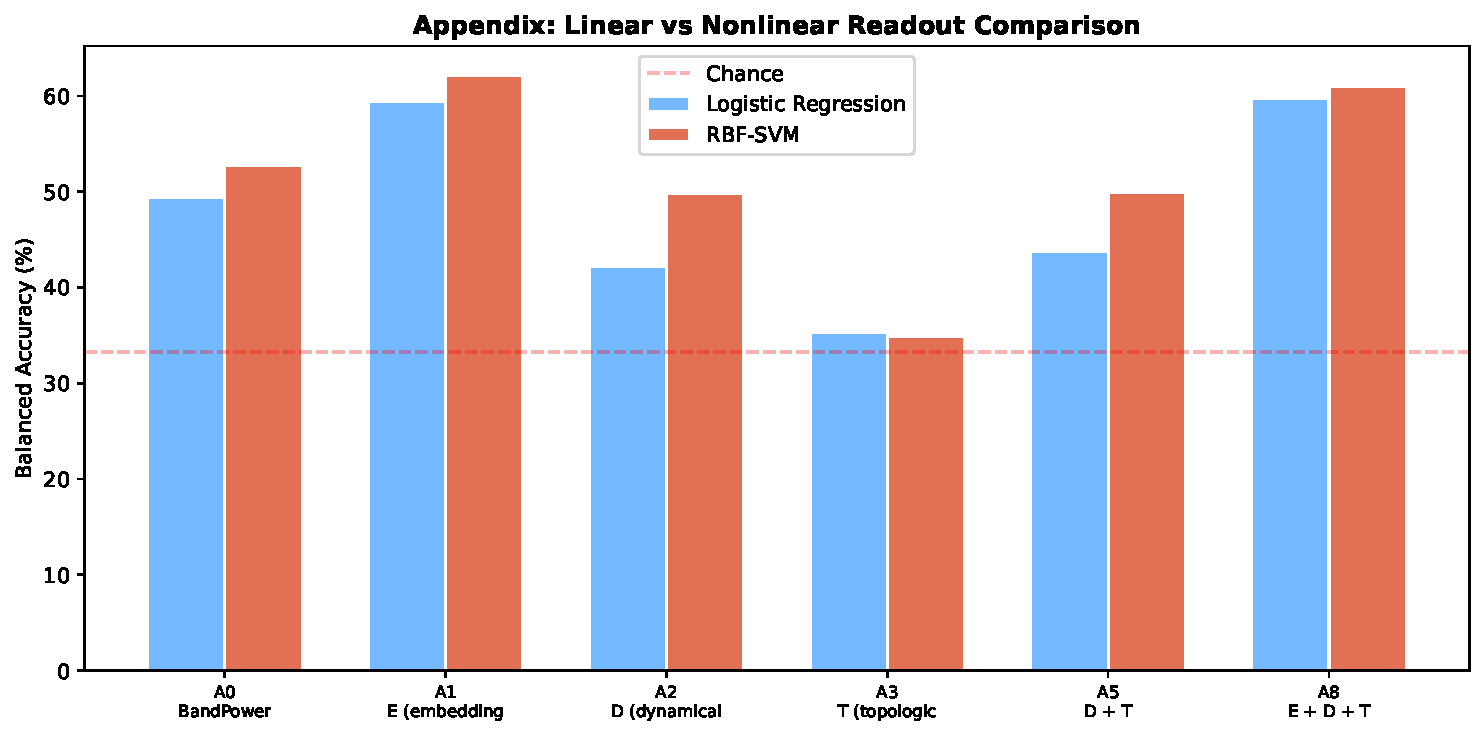
\includegraphics[width=\textwidth]{pictures/appendixA/ch5_fig_rbf_sensitivity.pdf}
    \caption{Archived linear (logistic regression) and nonlinear (RBF-SVM) readout comparison. The embedding mean changes from $59.4\%$ to $62.1\%$; the dynamical-summary mean changes from $42.2\%$ to $49.8\%$. These finite, post-hoc differences do not identify a uniquely nonlinear information source.}
    \label{fig:app_rbf_sensitivity}
\end{figure}


%% ═══════════════════════════════════════════════════════════════
%% SECTION A.4: CHAPTER 6 FIGURES
%% ═══════════════════════════════════════════════════════════════
\section{Chapter 6: Supplementary Raw Observations}
\label{app:ch6_figs}

The following eight archived figures display distributions, channel-index heterogeneity, population firing-rate summaries, within-epoch phase summaries, graph-derived quantities, and clinical metadata coverage. The seven experimental result figures (EXP-6.1 through EXP-6.7) are presented inline in Chapter~\ref{chap:dynamics}.

\begin{figure}[H]
    \centering
    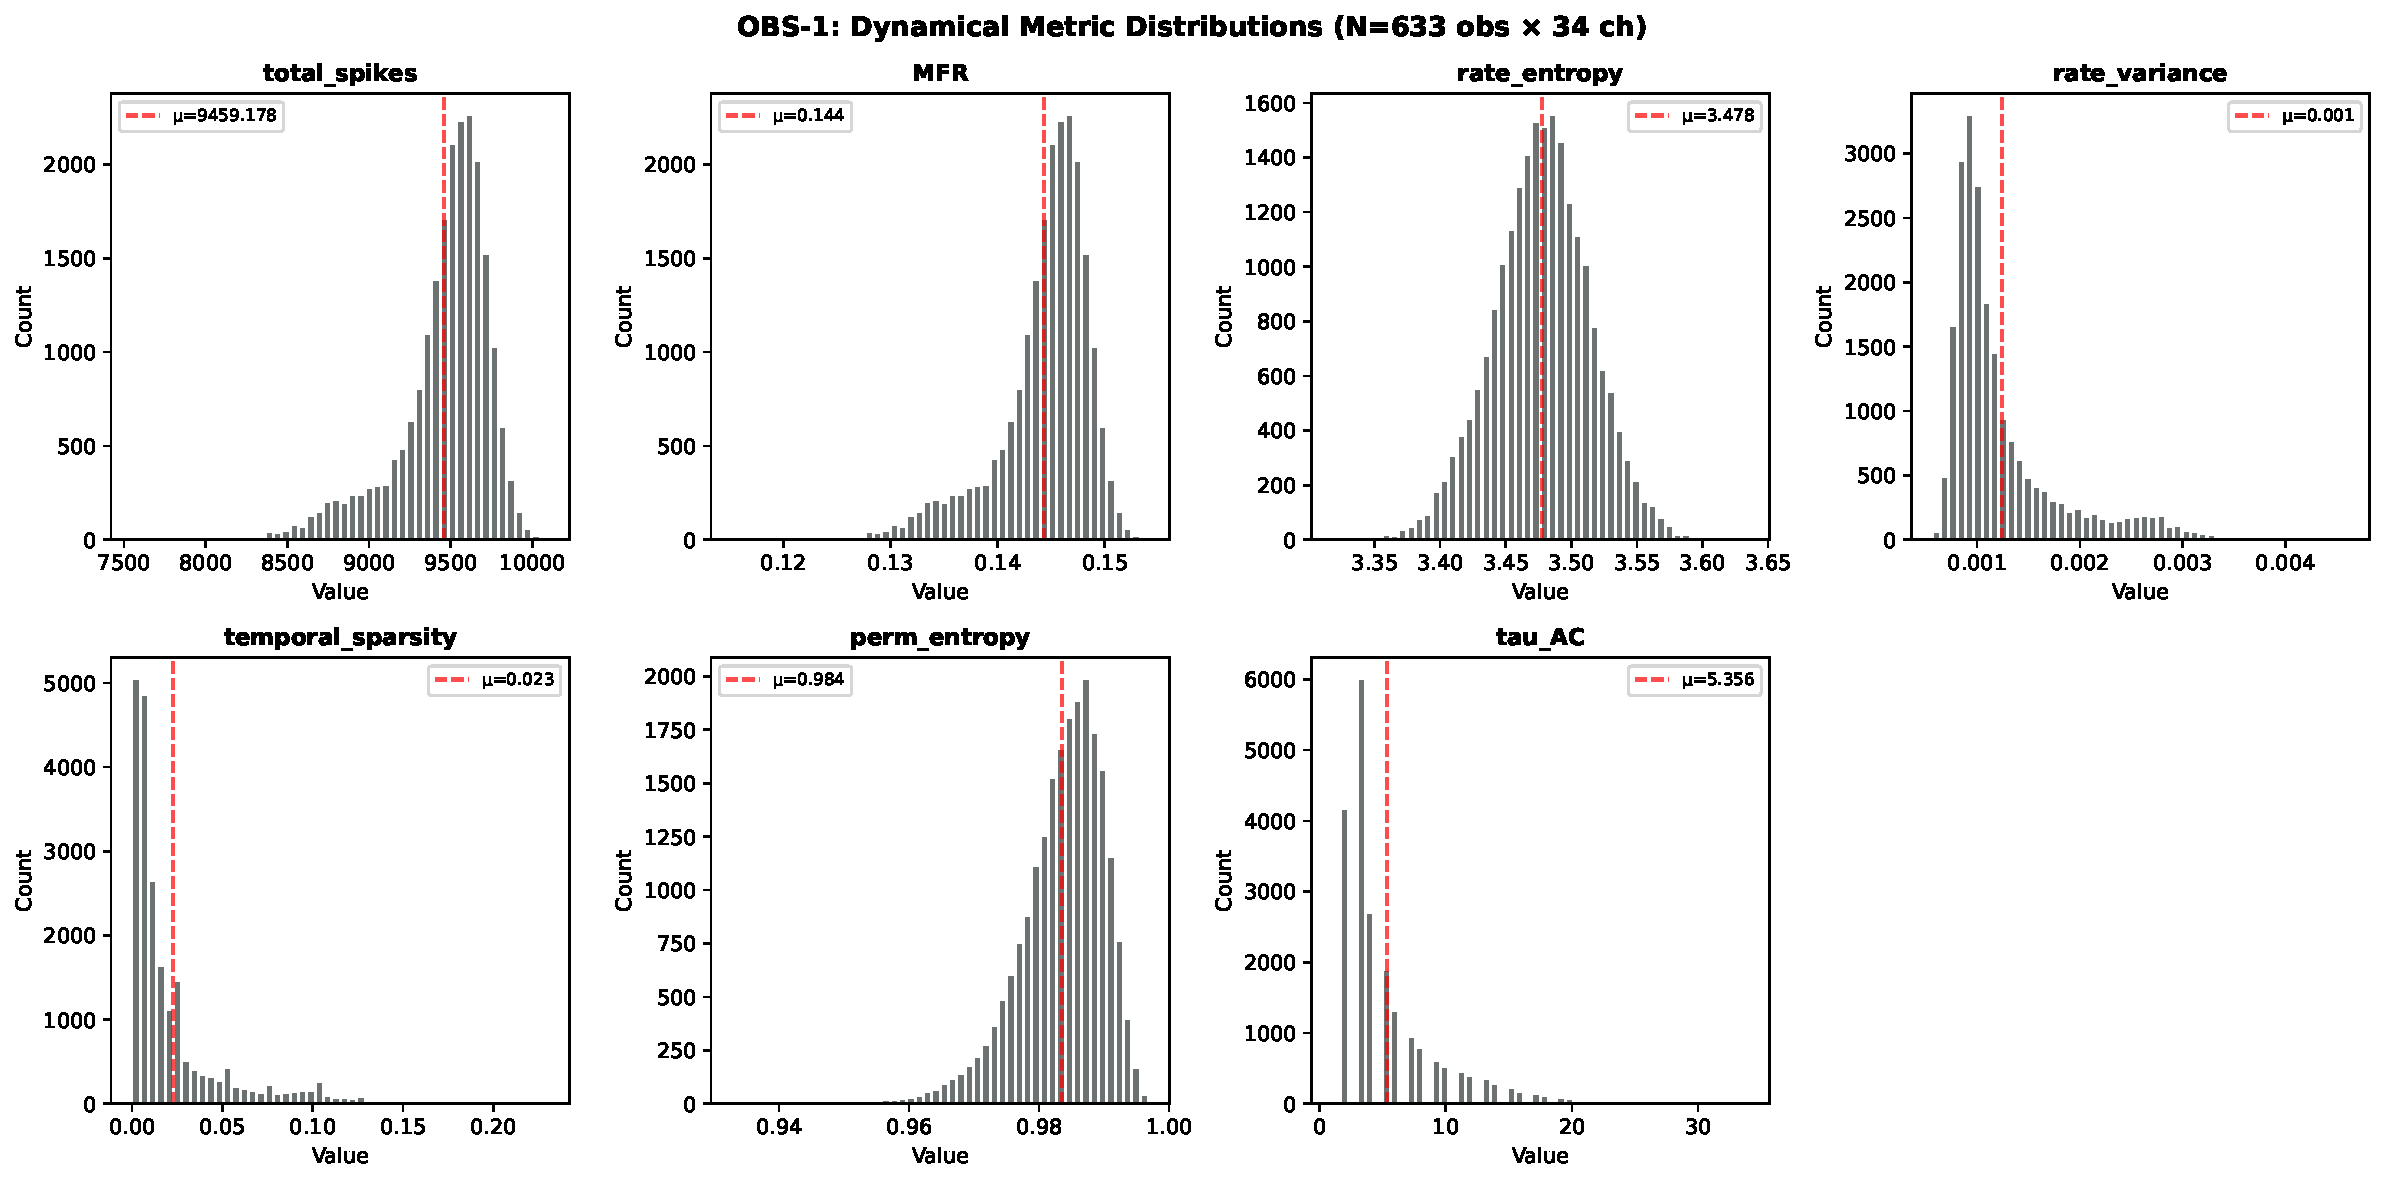
\includegraphics[width=\textwidth]{pictures/appendixA/obs01_metric_distributions.pdf}
    \caption{OBS-1: Dynamical metric distributions across all $633$ observations ($211$ subjects $\times$ $3$ conditions). Seven core metrics span different variability regimes: $\tau_{\text{AC}}$ (CV~$= 0.77$) and temporal sparsity (CV~$= 1.24$) show the highest variability; MFR (CV~$= 0.03$) and permutation entropy (CV~$= 0.007$) show the lowest.}
    \label{fig:app_ch6_obs01}
\end{figure}

\begin{figure}[H]
    \centering
    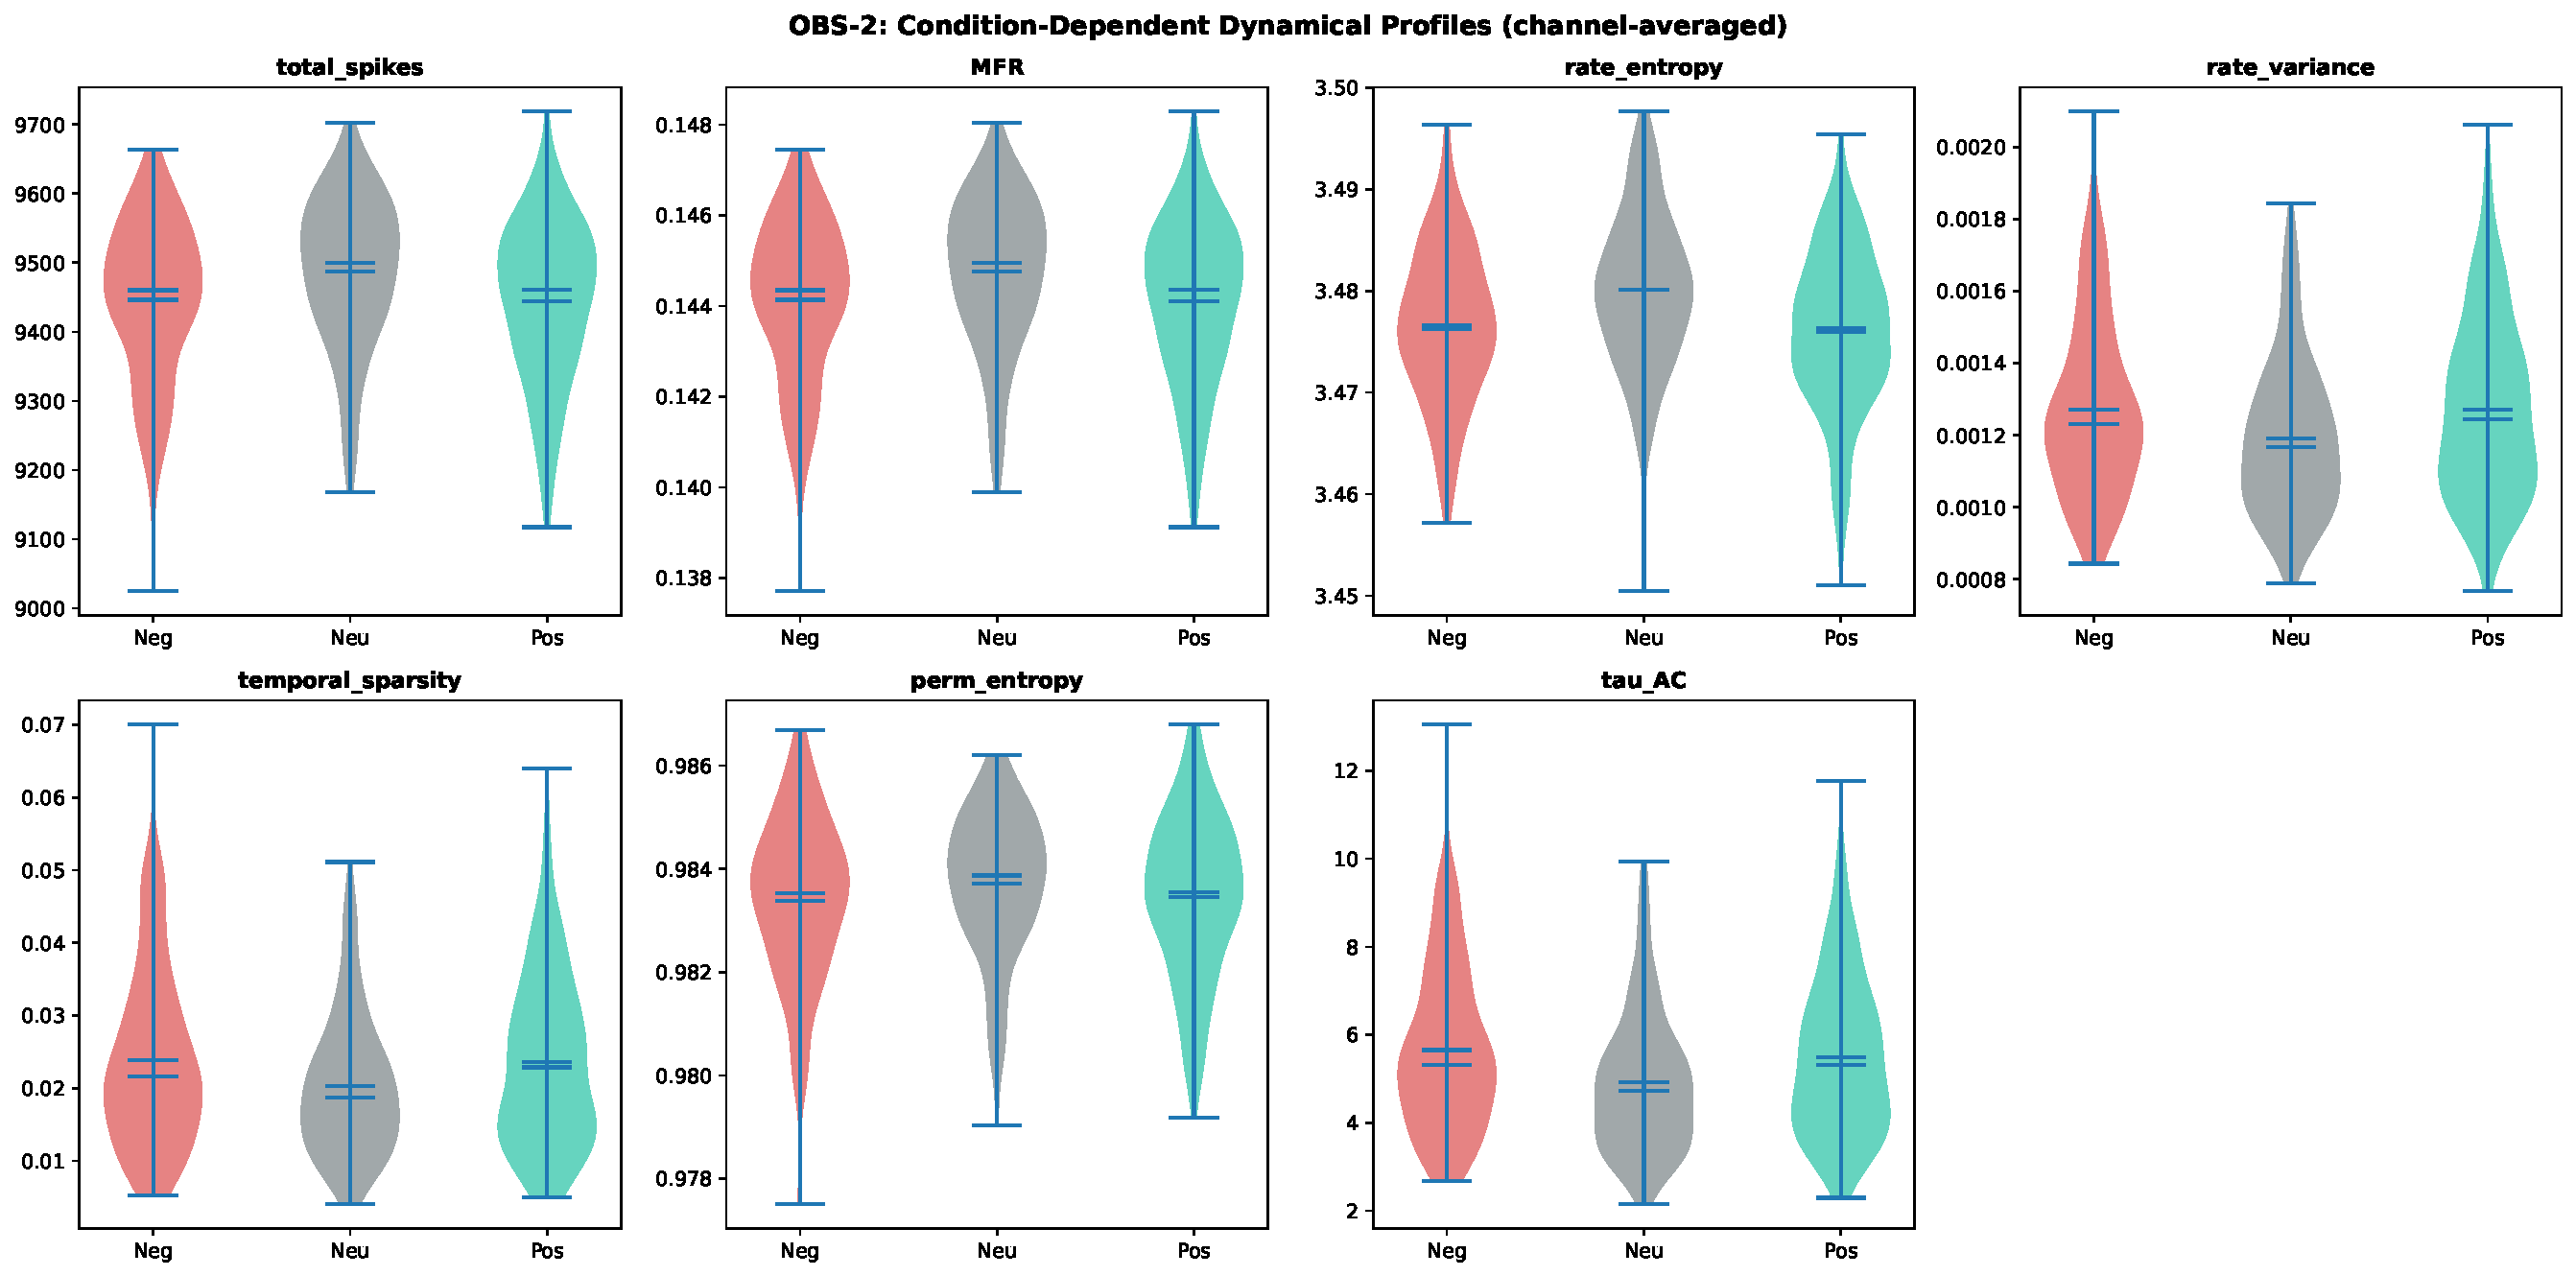
\includegraphics[width=\textwidth]{pictures/appendixA/obs02_condition_profiles.pdf}
    \caption{OBS-2: Archived condition-level dynamical summaries. Negative and Pleasant have similar means for the displayed metrics, while Neutral differs most for $\tau_{\text{AC}}$: Negative ($5.65$), Pleasant ($5.50$), and Neutral ($4.92$). No participant- or stimulus-level arousal scores were modeled, so the pattern cannot be attributed specifically to arousal.}
    \label{fig:app_ch6_obs02}
\end{figure}

\begin{figure}[H]
    \centering
    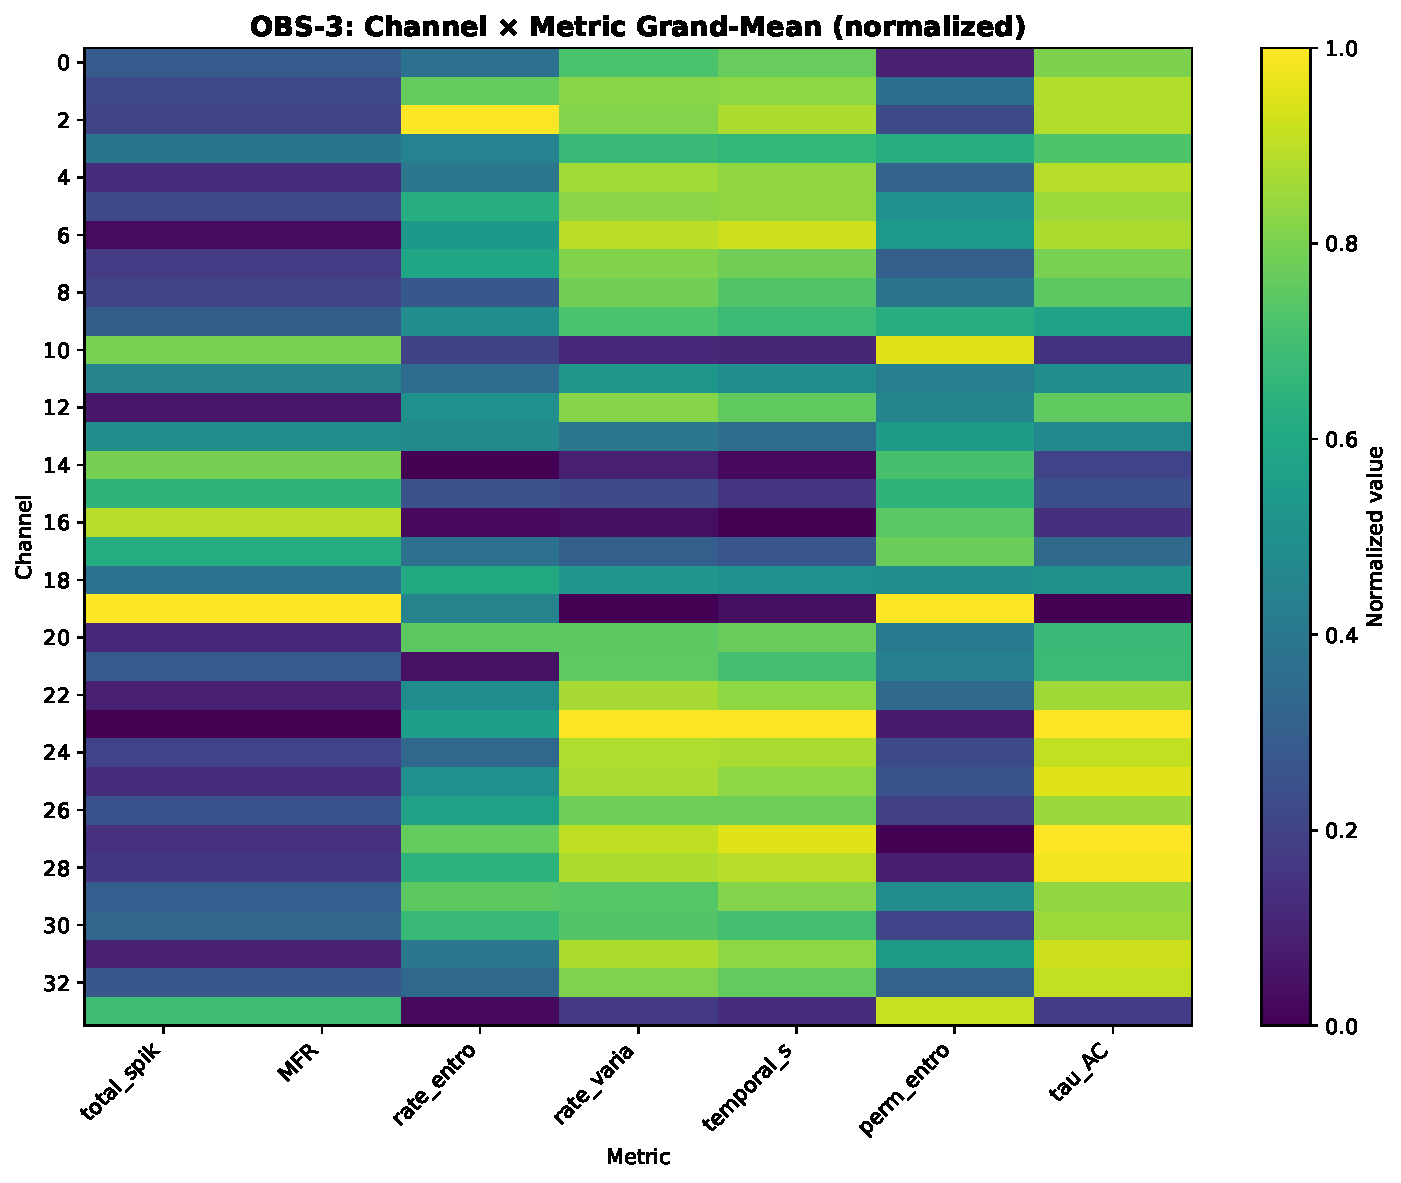
\includegraphics[width=\textwidth]{pictures/appendixA/obs03_channel_heterogeneity.pdf}
    \caption{OBS-3: Per-channel-index dynamical summaries. Temporal sparsity and $\tau_{\text{AC}}$ have maximum-to-minimum ratios of $2.54\times$ and $1.56\times$, respectively. Rate-entropy and permutation-entropy means vary less across the unlabeled channel indices.}
    \label{fig:app_ch6_obs03}
\end{figure}

\begin{figure}[H]
    \centering
    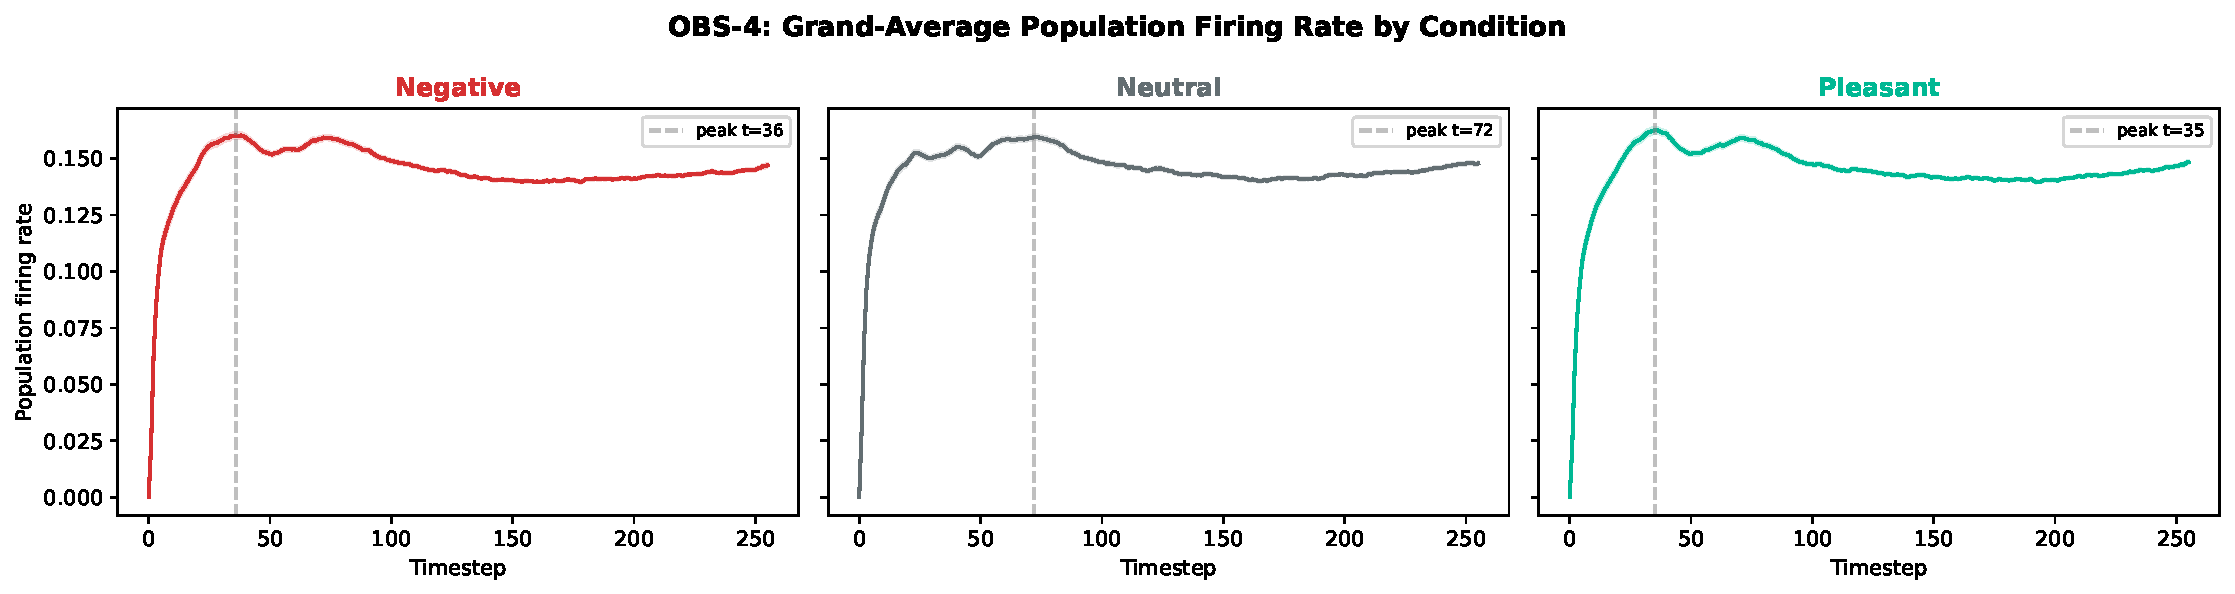
\includegraphics[width=\textwidth]{pictures/appendixA/obs04_firing_rate_timecourses.pdf}
    \caption{OBS-4: Grand-average reservoir population firing-rate traces. Negative and Pleasant peak at $t\approx35$--$36$, while Neutral peaks at $t=72$; the Pleasant peak-to-final ratio is $1.11$. These sample timings are descriptive and are not a validated measure of emotional salience.}
    \label{fig:app_ch6_obs04}
\end{figure}

\begin{figure}[H]
    \centering
    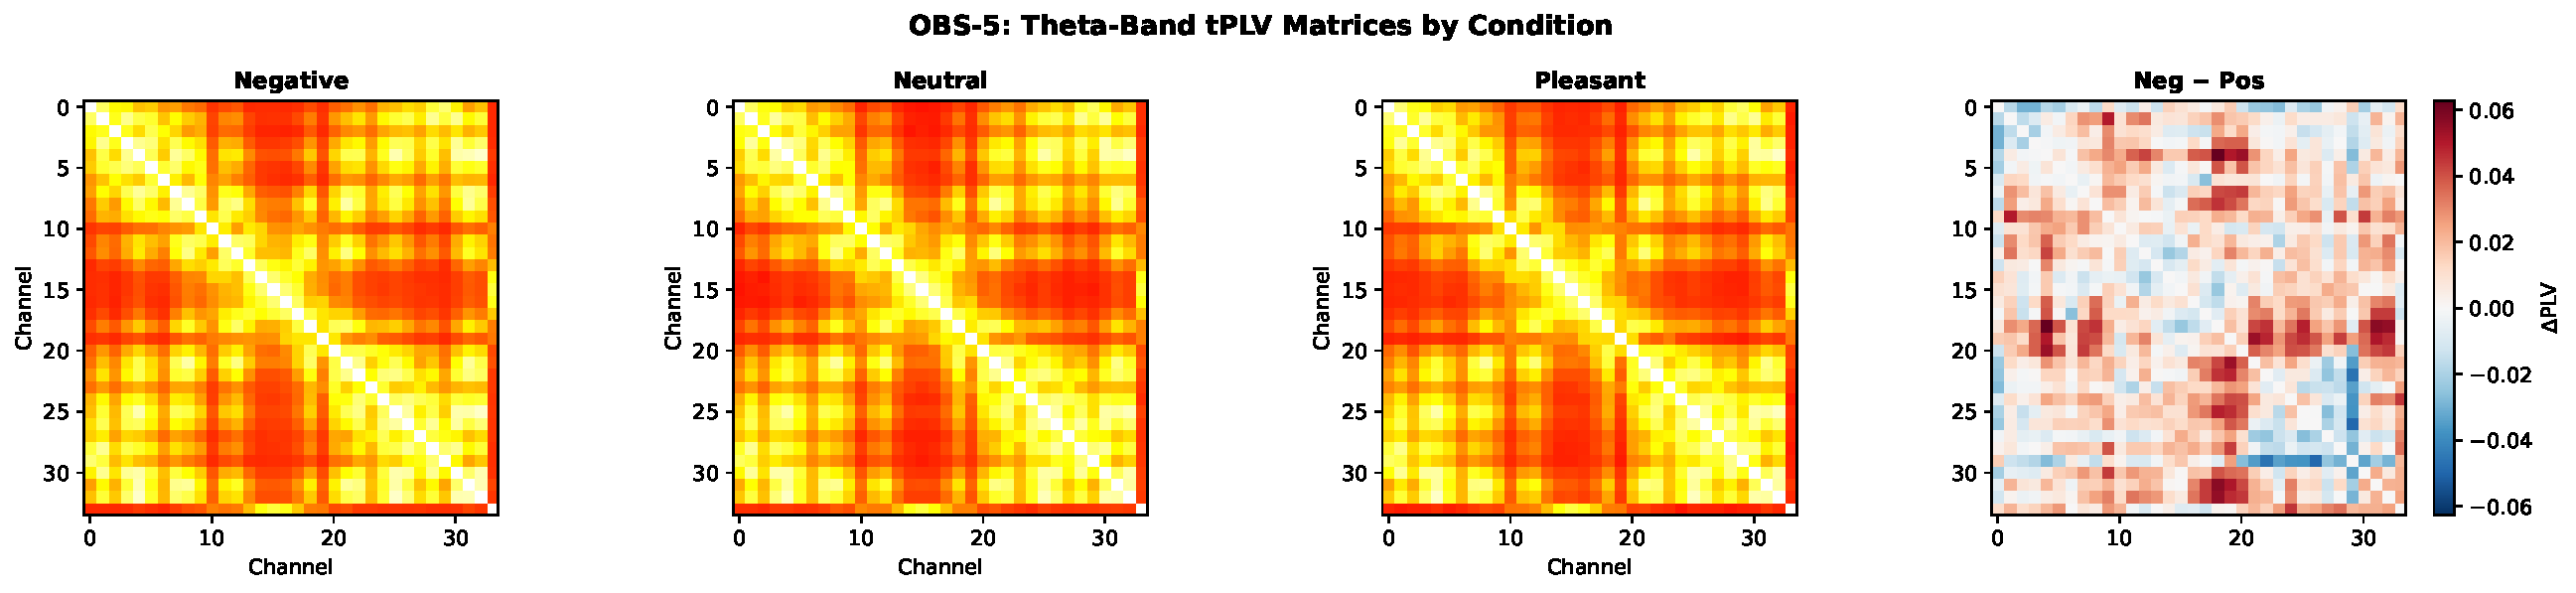
\includegraphics[width=\textwidth]{pictures/appendixA/obs05_tplv_connectivity.pdf}
    \caption{OBS-5: Archived theta-band within-epoch phase-concentration summaries. The displayed mean PLV values are Negative ($0.635$), Neutral ($0.632$), and Pleasant ($0.626$); the Negative--Pleasant mean $|\Delta\mathrm{PLV}|$ is $0.016$ (maximum $0.063$). With one trial-averaged epoch per participant--condition and unlabeled channels, these values are not interpreted as physiological connectivity.}
    \label{fig:app_ch6_obs05}
\end{figure}

\begin{figure}[H]
    \centering
    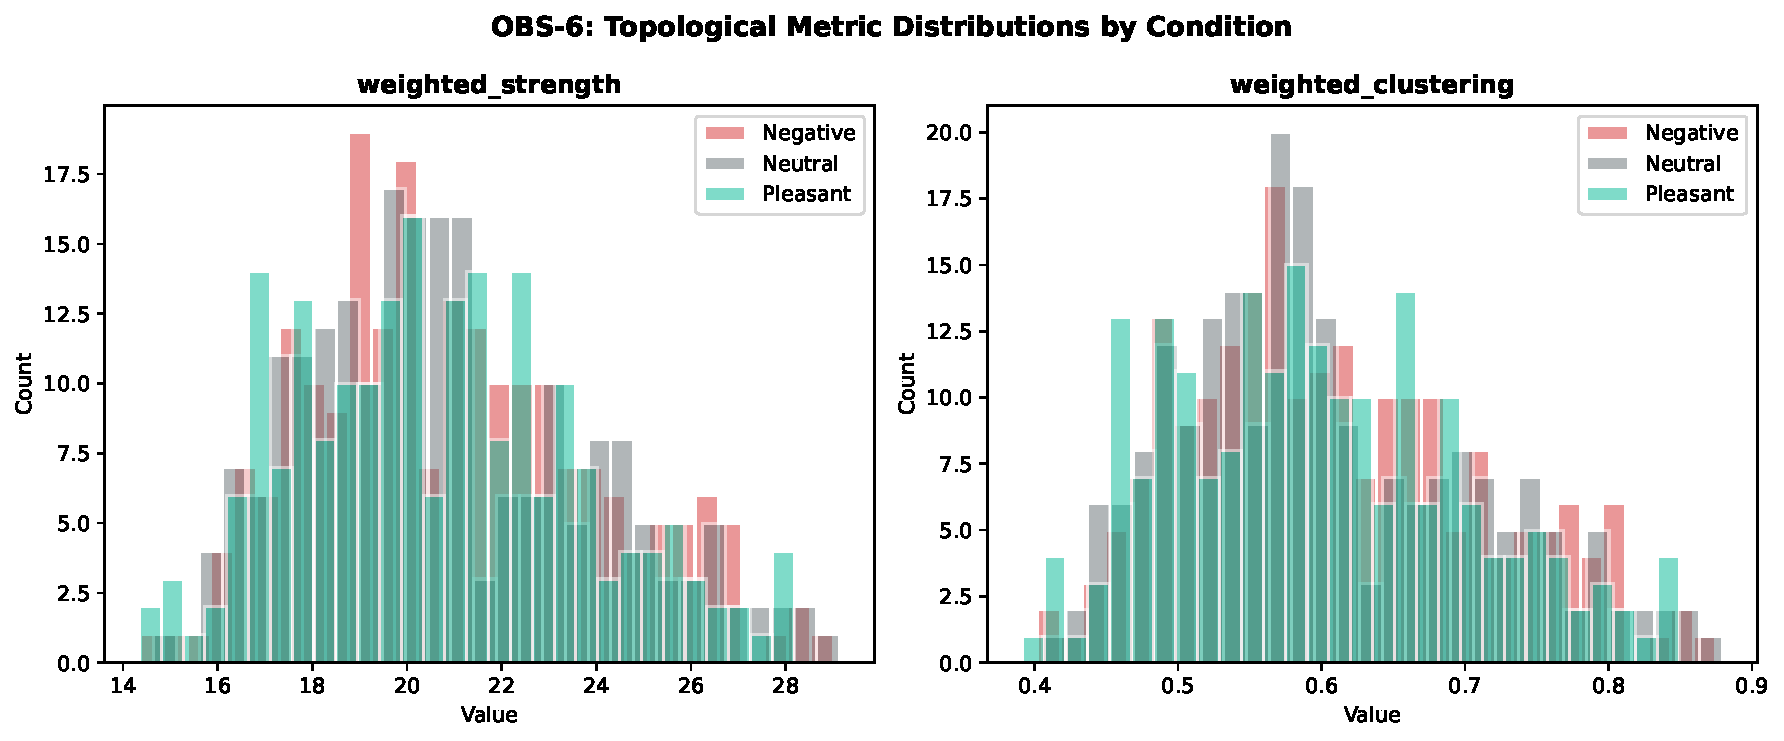
\includegraphics[width=\textwidth]{pictures/appendixA/obs06_topological_distributions.pdf}
    \caption{OBS-6: Archived graph-summary distributions. Weighted node strength ranges from $5.9$ to $30.8$, and weighted clustering from $0.21$ to $0.91$. The channel-index ranges permit the numerical association analysis in Chapter~\ref{chap:synthesis}, but they have no anatomical interpretation.}
    \label{fig:app_ch6_obs06}
\end{figure}

\begin{figure}[H]
    \centering
    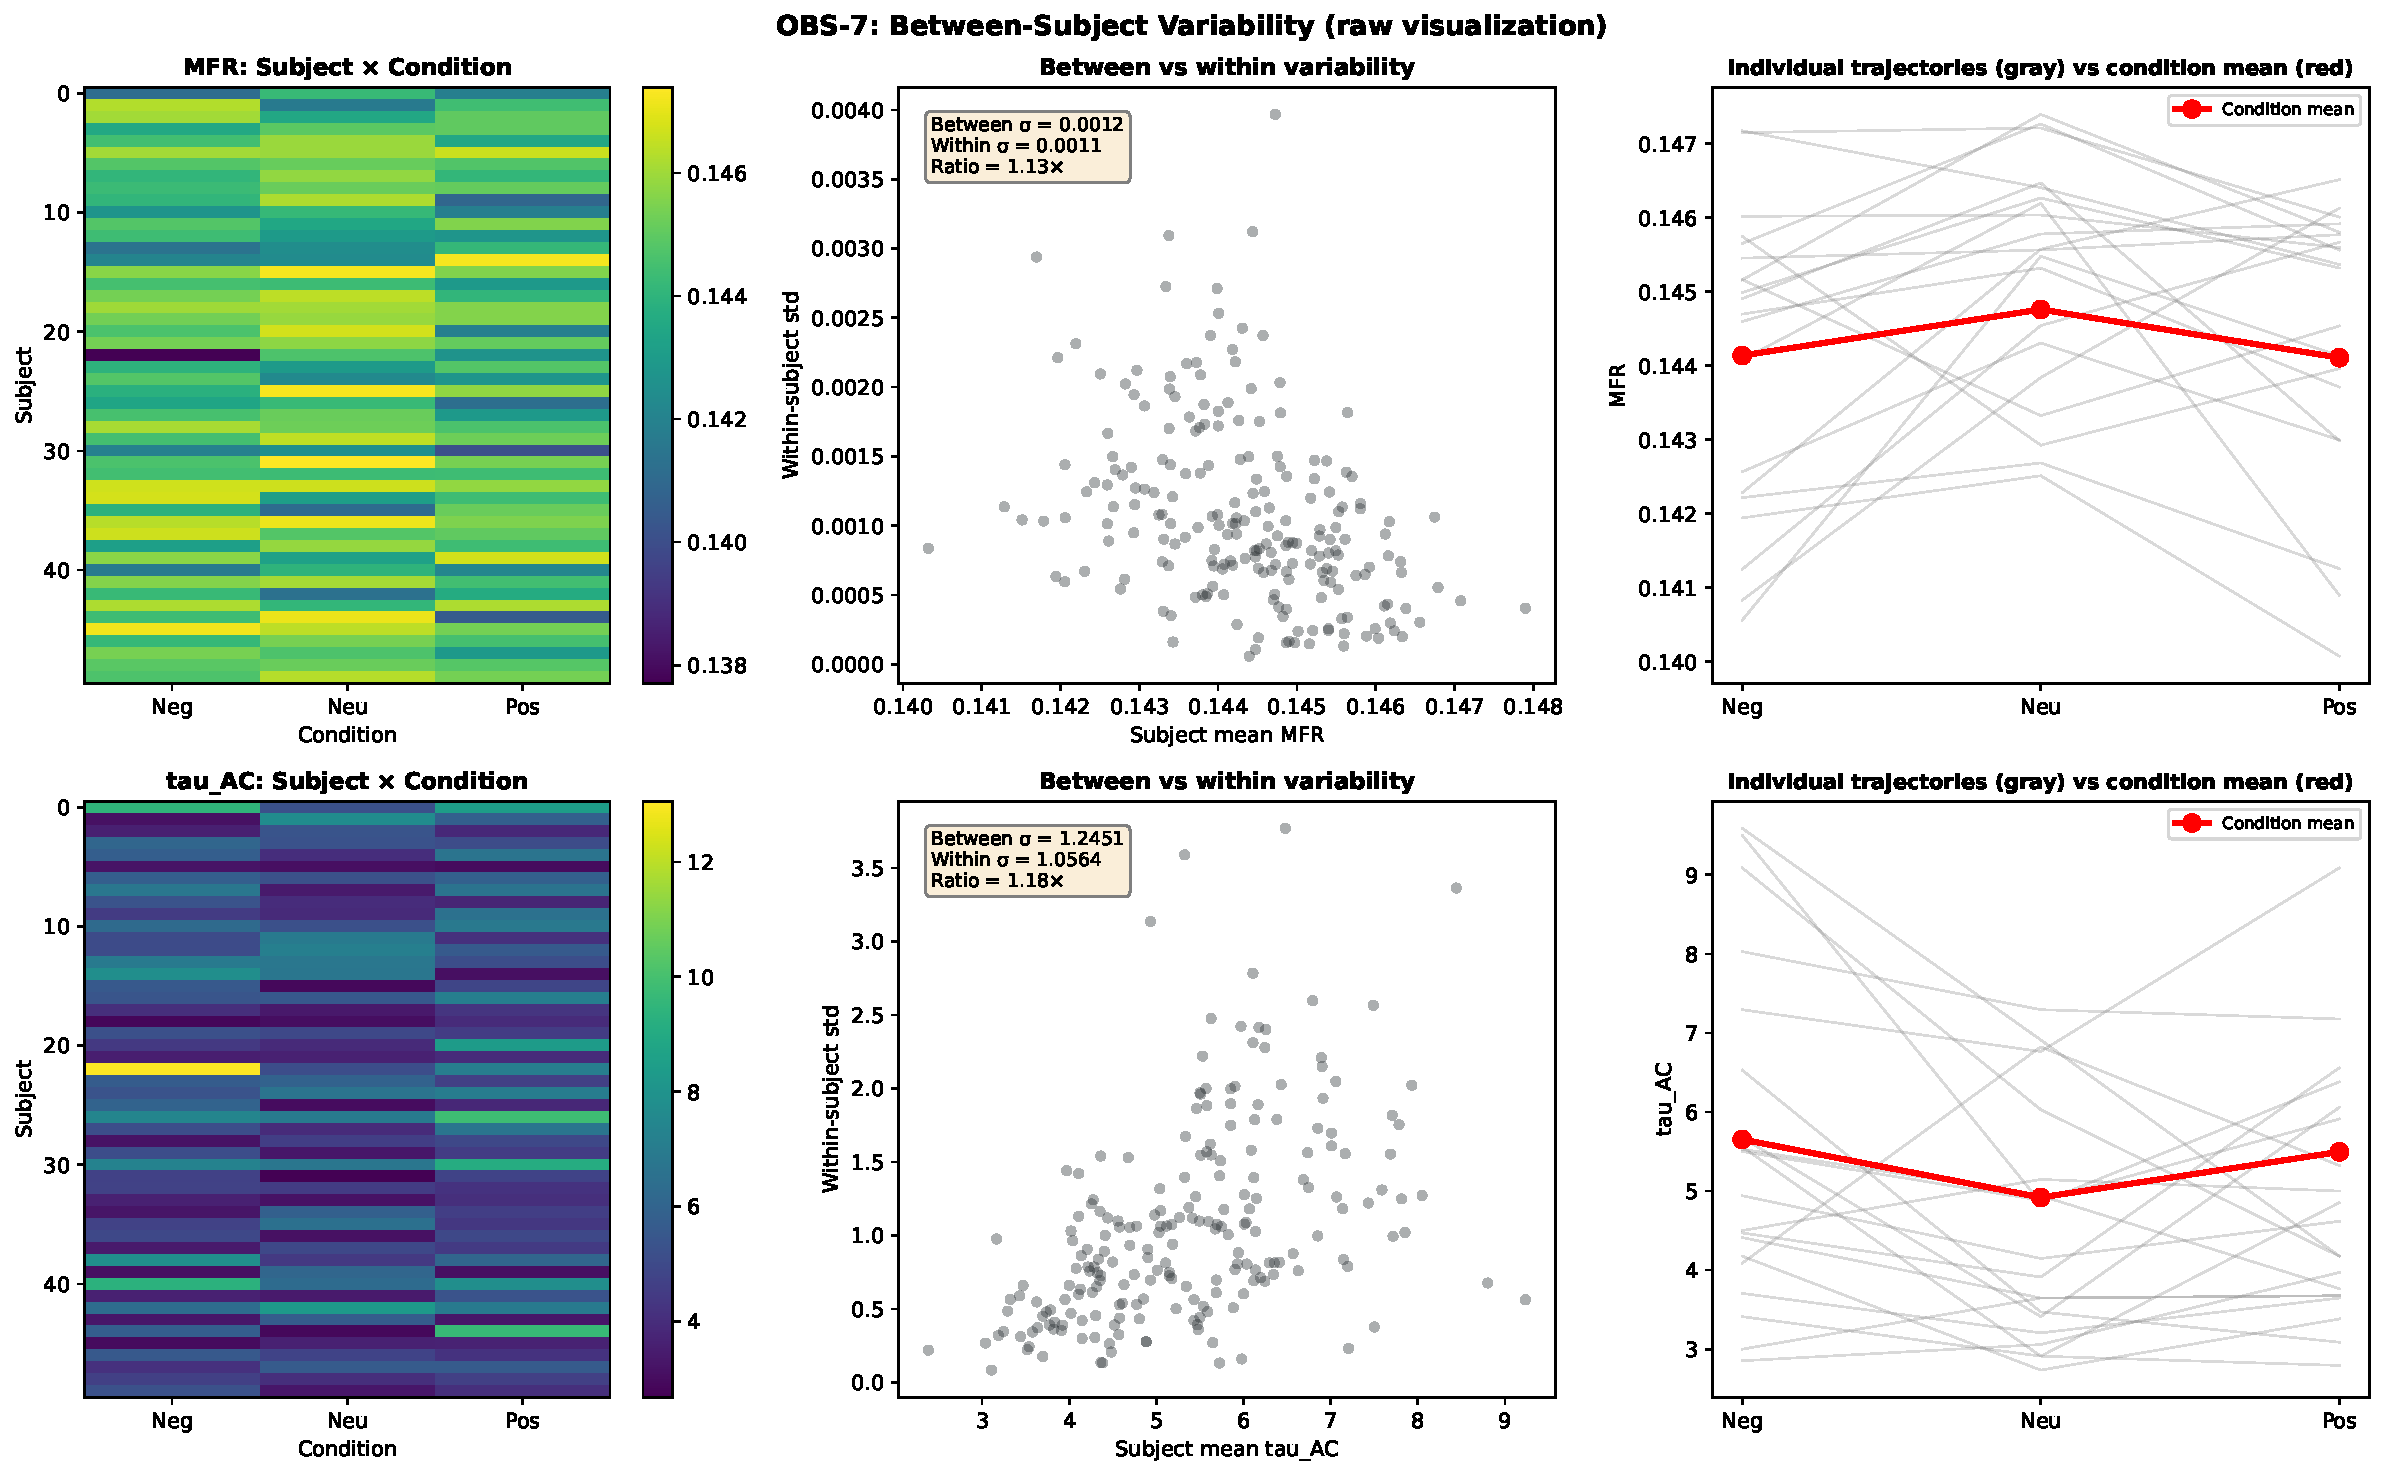
\includegraphics[width=\textwidth]{pictures/appendixA/obs07_subject_variability.pdf}
    \caption{OBS-7: Archived between-participant and within-participant variability summaries. The reported rate-entropy and permutation-entropy ratios are $0.87$ and $0.90$. These descriptive ratios are not test--retest reliabilities and are not directly comparable with the globally fitted BSC$_6$ PCA decomposition.}
    \label{fig:app_ch6_obs07}
\end{figure}

\begin{figure}[H]
    \centering
    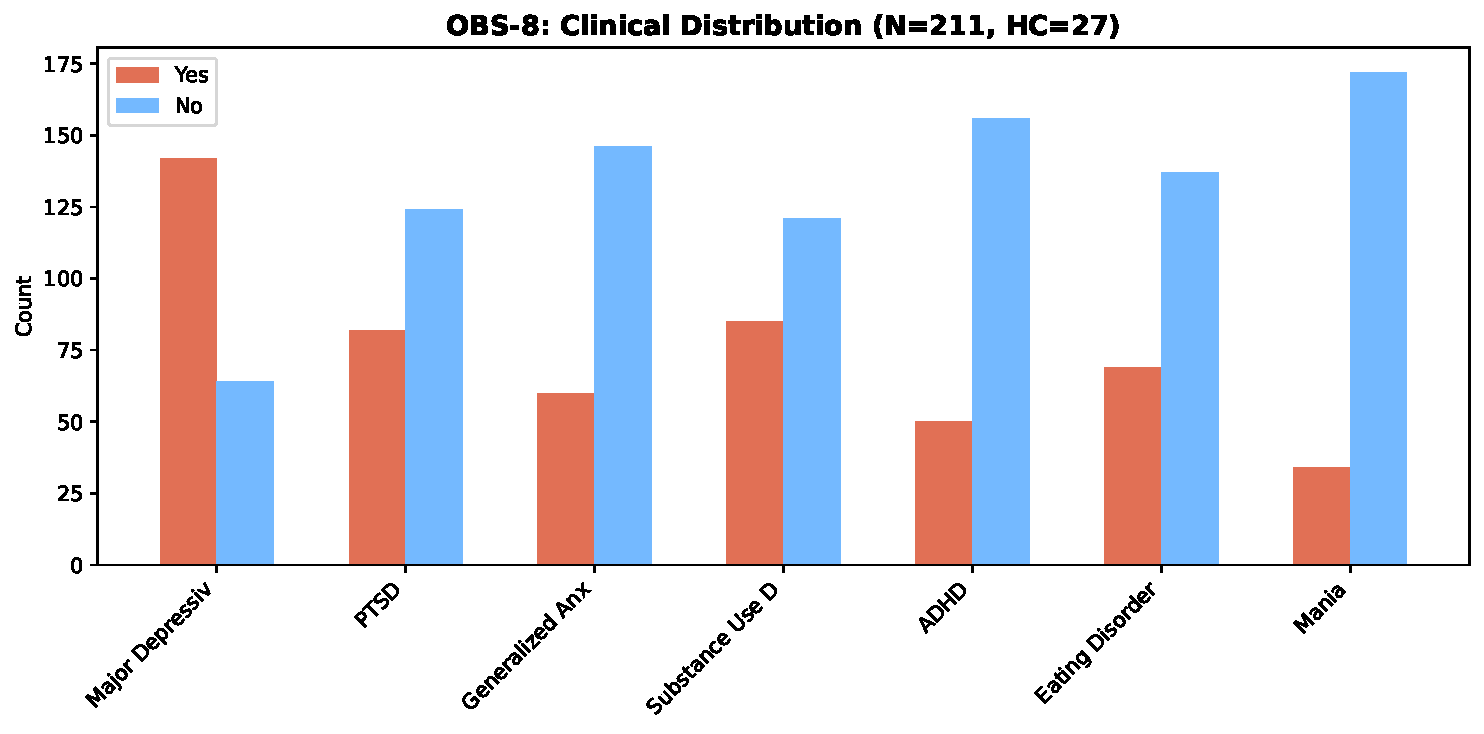
\includegraphics[width=\textwidth]{pictures/appendixA/obs08_clinical_distribution.pdf}
    \caption{OBS-8: Clinical metadata coverage. Complete five-diagnosis data are available for 206 of 211 subjects. MDD: 142 vs.\ 64; PTSD: 82 vs.\ 124; SUD: 85 vs.\ 121. Twenty-two complete cases are negative for all five primary diagnoses. The supplied full-panel comorbidity variable has mean 2.8 (rounded).}
    \label{fig:app_ch6_obs08}
\end{figure}



%% ═══════════════════════════════════════════════════════════════
%% SECTION A.5: CHAPTER 7
%% ═══════════════════════════════════════════════════════════════
\section{Chapter 7: Structure-Function Coupling}
\label{app:ch7_figs}

The five three-class coupling experiment figures (EXP-7.1 through EXP-7.5) are presented inline in Chapter~\ref{chap:synthesis}, Section~\ref{sec:ch7_3class}. The fourteen four-class coupling figures are presented inline in Sections~\ref{sec:exp7_coupling}--\ref{sec:exp7_augmentation} of the same chapter. No supplementary coupling figures are required.


\end{document}
